%% Run LaTeX on this file several times to get Table of Contents,
%% cross-references, and citations.

\documentclass[11pt]{book}
\usepackage{gvv-book}
%\usepackage{Wiley-AuthoringTemplate}
\usepackage[sectionbib,authoryear]{natbib}% for name-date citation comment the below line
%\usepackage[sectionbib,numbers]{natbib}% for numbered citation comment the above line

%%********************************************************************%%
%%       How many levels of section head would you like numbered?     %%
%% 0= no section numbers, 1= section, 2= subsection, 3= subsubsection %%
\setcounter{secnumdepth}{3}
%%********************************************************************%%
%%**********************************************************************%%
%%     How many levels of section head would you like to appear in the  %%
%%				Table of Contents?			%%
%% 0= chapter, 1= section, 2= subsection, 3= subsubsection titles.	%%
\setcounter{tocdepth}{2}
%%**********************************************************************%%

%\includeonly{ch01}
\makeindex

\begin{document}

\frontmatter
%%%%%%%%%%%%%%%%%%%%%%%%%%%%%%%%%%%%%%%%%%%%%%%%%%%%%%%%%%%%%%%%
%% Title Pages
%% Wiley will provide title and copyright page, but you can make
%% your own titlepages if you'd like anyway
%% Setting up title pages, type in the appropriate names here:

\booktitle{Machine Learning}

\subtitle{Through Practise}

\AuAff{G. V. V. Sharma}


%% \\ will start a new line.
%% You may add \affil{} for affiliation, ie,
%\authors{Robert M. Groves\\
%\affil{Universitat de les Illes Balears}
%Floyd J. Fowler, Jr.\\
%\affil{University of New Mexico}
%}

%% Print Half Title and Title Page:
%\halftitlepage
\titlepage

%%%%%%%%%%%%%%%%%%%%%%%%%%%%%%%%%%%%%%%%%%%%%%%%%%%%%%%%%%%%%%%%
%% Copyright Page

\begin{copyrightpage}{2023}
%Title, etc
\end{copyrightpage}

% Note, you must use \ to start indented lines, ie,
% 
% \begin{copyrightpage}{2004}
% Survey Methodology / Robert M. Groves . . . [et al.].
% \       p. cm.---(Wiley series in survey methodology)
% \    ``Wiley-Interscience."
% \    Includes bibliographical references and index.
% \    ISBN 0-471-48348-6 (pbk.)
% \    1. Surveys---Methodology.  2. Social 
% \  sciences---Research---Statistical methods.  I. Groves, Robert M.  II. %
% Series.\\

% HA31.2.S873 2004
% 001.4'33---dc22                                             2004044064
% \end{copyrightpage}

%%%%%%%%%%%%%%%%%%%%%%%%%%%%%%%%%%%%%%%%%%%%%%%%%%%%%%%%%%%%%%%%
%% Only Dedication (optional) 

%\dedication{To my parents}

\tableofcontents

%\listoffigures %optional
%\listoftables  %optional

%% or Contributor Page for edited books
%% before \tableofcontents

%%%%%%%%%%%%%%%%%%%%%%%%%%%%%%%%%%%%%%%%%%%%%%%%%%%%%%%%%%%%%%%%
%  Contributors Page for Edited Book
%%%%%%%%%%%%%%%%%%%%%%%%%%%%%%%%%%%%%%%%%%%%%%%%%%%%%%%%%%%%%%%%

% If your book has chapters written by different authors,
% you'll need a Contributors page.

% Use \begin{contributors}...\end{contributors} and
% then enter each author with the \name{} command, followed
% by the affiliation information.

% \begin{contributors}
% \name{Masayki Abe,} Fujitsu Laboratories Ltd., Fujitsu Limited, Atsugi, Japan
%
% \name{L. A. Akers,} Center for Solid State Electronics Research, Arizona State University, Tempe, Arizona
%
% \name{G. H. Bernstein,} Department of Electrical and Computer Engineering, University of Notre Dame, Notre Dame, South Bend, Indiana; formerly of
% Center for Solid State Electronics Research, Arizona
% State University, Tempe, Arizona 
% \end{contributors}

%%%%%%%%%%%%%%%%%%%%%%%%%%%%%%%%%%%%%%%%%%%%%%%%%%%%%%%%%%%%%%%%
% Optional Foreword:

%\begin{foreword}
%\lipsum[1-2]
%\end{foreword}

%%%%%%%%%%%%%%%%%%%%%%%%%%%%%%%%%%%%%%%%%%%%%%%%%%%%%%%%%%%%%%%%
% Optional Preface:

%\begin{preface}
%\lipsum[1-1]
%\prefaceauthor{}
%\where{place\\
% date}
%\end{preface}

% ie,
% \begin{preface}
% This is an example preface.
% \prefaceauthor{R. K. Watts}
% \where{Durham, North Carolina\\
% September, 2004}

%%%%%%%%%%%%%%%%%%%%%%%%%%%%%%%%%%%%%%%%%%%%%%%%%%%%%%%%%%%%%%%%
% Optional Acknowledgments:

%\acknowledgments
%\lipsum[1-2]
%\authorinitials{I. R. S.}  

%%%%%%%%%%%%%%%%%%%%%%%%%%%%%%%%
%% Glossary Type of Environment:

% \begin{glossary}
% \term{<term>}{<description>}
% \end{glossary}

%%%%%%%%%%%%%%%%%%%%%%%%%%%%%%%%
%\begin{acronyms}
%\acro{ASTA}{Arrivals See Time Averages}
%\acro{BHCA}{Busy Hour Call Attempts}
%\acro{BR}{Bandwidth Reservation}
%\acro{b.u.}{bandwidth unit(s)}
%\acro{CAC}{Call / Connection Admission Control}
%\acro{CBP}{Call Blocking Probability(-ies)}
%\acro{CCS}{Centum Call Seconds}
%\acro{CDTM}{Connection Dependent Threshold Model}
%\acro{CS}{Complete Sharing}
%\acro{DiffServ}{Differentiated Services}
%\acro{EMLM}{Erlang Multirate Loss Model}
%\acro{erl}{The Erlang unit of traffic-load}
%\acro{FIFO}{First in - First out}
%\acro{GB}{Global balance}
%\acro{GoS}{Grade of Service}
%\acro{ICT}{Information and Communication Technology}
%\acro{IntServ}{Integrated Services}
%\acro{IP}{Internet Protocol}
%\acro{ITU-T}{International Telecommunication Unit -- Standardization sector}
%\acro{LB}{Local balance}
%\acro{LHS}{Left hand side}
%\acro{LIFO}{Last in - First out}
%\acro{MMPP}{Markov Modulated Poisson Process}
%\acro{MPLS}{Multiple Protocol Labeling Switching}
%\acro{MRM}{Multi-Retry Model}
%\acro{MTM}{Multi-Threshold Model}
%\acro{PASTA}{Poisson Arrivals See Time Averages}
%\acro{PDF}{Probability Distribution Function}
%\acro{pdf}{probability density function}
%\acro{PFS}{Product Form Solution}
%\acro{QoS}{Quality of Service}
%\acro{r.v.}{random variable(s)}
%\acro{RED}{random early detection}
%\acro{RHS}{Right hand side}
%\acro{RLA}{Reduced Load Approximation}
%\acro{SIRO}{service in random order}
%\acro{SRM}{Single-Retry Model}
%\acro{STM}{Single-Threshold Model}
%\acro{TCP}{Transport Control Protocol}
%\acro{TH}{Threshold(s)}
%\acro{UDP}{User Datagram Protocol}
%\end{acronyms}

\setcounter{page}{1}

\begin{introduction}
This book introduces machine learning through simple examples

\end{introduction}

\mainmatter
\chapter{Least Squares}
\begin{enumerate}[label=\thesection.\arabic*,ref=\thesection.\theenumi]
\item Find the shortest distance between the lines\\  $\overrightarrow{r}=(\hat{i}+2\hat{j}+\hat{k})+\lambda(\hat{i}-\hat{j}+\hat{k})$ and \\$\overrightarrow{r}=2\hat{i}-\hat{j}-\hat{k}+\mu(2\hat{i}+\hat{j}+2\hat{k})$
\item Find the shortest distance between the lines\\
$ \frac{x+1}{7}=\frac{y+1}{-6}=\frac{z+1}{1}$ and $ \frac{x-3}{1}=\frac{y-5}{-2}=\frac{z-7}{1}$ 
    \solution
		\iffalse
\documentclass[journal,12pt,twocolumn]{IEEEtran}
\usepackage{romannum}
\usepackage{float}
\usepackage{setspace}
\usepackage{gensymb}
\singlespacing
\usepackage[cmex10]{amsmath}
\usepackage{amsthm}
\usepackage{mathrsfs}
\usepackage{txfonts}
\usepackage{stfloats}
\usepackage{bm}
\usepackage{cite}
\usepackage{cases}
\usepackage{subfig}
\usepackage{longtable}
\usepackage{multirow}
\usepackage{enumitem}
\usepackage{mathtools}
\usepackage{steinmetz}
\usepackage{tikz}
\usepackage{circuitikz}
\usepackage{verbatim}
\usepackage{tfrupee}
\usepackage[breaklinks=true]{hyperref}
\usepackage{tkz-euclide}
\usetikzlibrary{calc,math}
\usepackage{listings}
    \usepackage{color}                                            %%
    \usepackage{array}                                            %%
    \usepackage{longtable}                                        %%
    \usepackage{calc}                                             %%
    \usepackage{multirow}                                         %%
    \usepackage{hhline}                                           %%
    \usepackage{ifthen}                                           %%
  %optionally (for landscape tables embedded in another document): %%
    \usepackage{lscape}     
\usepackage{multicol}
\usepackage{chngcntr}
\DeclareMathOperator*{\Res}{Res}
\renewcommand\thesection{\arabic{section}}
\renewcommand\thesubsection{\thesection.\arabic{subsection}}
\renewcommand\thesubsubsection{\thesubsection.\arabic{subsubsection}}

\renewcommand\thesectiondis{\arabic{section}}
\renewcommand\thesubsectiondis{\thesectiondis.\arabic{subsection}}
\renewcommand\thesubsubsectiondis{\thesubsectiondis.\arabic{subsubsection}}

% correct bad hyphenation here
\hyphenation{op-tical net-works semi-conduc-tor}
\def\inputGnumericTable{}                                 %%

\lstset{
frame=single, 
breaklines=true,
columns=fullflexible
}

\begin{document}


\newtheorem{theorem}{Theorem}[section]
\newtheorem{problem}{Problem}
\newtheorem{proposition}{Proposition}[section]
\newtheorem{lemma}{Lemma}[section]
\newtheorem{corollary}[theorem]{Corollary}
\newtheorem{example}{Example}[section]
\newtheorem{definition}[problem]{Definition}
\newcommand{\BEQA}{\begin{eqnarray}}
\newcommand{\EEQA}{\end{eqnarray}}
\newcommand{\define}{\stackrel{\triangle}{=}}

\bibliographystyle{IEEEtran}
\providecommand{\mbf}{\mathbf}
\providecommand{\pr}[1]{\ensuremath{\Pr\left(#1\right)}}
\providecommand{\qfunc}[1]{\ensuremath{Q\left(#1\right)}}
\providecommand{\sbrak}[1]{\ensuremath{{}\left[#1\right]}}
\providecommand{\lsbrak}[1]{\ensuremath{{}\left[#1\right.}}
\providecommand{\rsbrak}[1]{\ensuremath{{}\left.#1\right]}}
\providecommand{\brak}[1]{\ensuremath{\left(#1\right)}}
\providecommand{\lbrak}[1]{\ensuremath{\left(#1\right.}}
\providecommand{\rbrak}[1]{\ensuremath{\left.#1\right)}}
\providecommand{\cbrak}[1]{\ensuremath{\left\{#1\right\}}}
\providecommand{\lcbrak}[1]{\ensuremath{\left\{#1\right.}}
\providecommand{\rcbrak}[1]{\ensuremath{\left.#1\right\}}}
\theoremstyle{remark}
\newtheorem{rem}{Remark}
\newcommand{\sgn}{\mathop{\mathrm{sgn}}}
\providecommand{\abs}[1]{\left\vert#1\right\vert}
\providecommand{\res}[1]{\Res\displaylimits_{#1}} 
\providecommand{\norm}[1]{\left\lVert#1\right\rVert}
\providecommand{\mtx}[1]{\mathbf{#1}}
\providecommand{\mean}[1]{E\left[ #1 \right]}
\providecommand{\fourier}{\overset{\mathcal{F}}{ \rightleftharpoons}}
\providecommand{\system}{\overset{\mathcal{H}}{ \longleftrightarrow}}
\newcommand{\solution}{\noindent \textbf{Solution: }}
\newcommand{\cosec}{\,\text{cosec}\,}
\providecommand{\dec}[2]{\ensuremath{\overset{#1}{\underset{#2}{\gtrless}}}}
\newcommand{\myvec}[1]{\ensuremath{\begin{pmatrix}#1\end{pmatrix}}}
\newcommand{\mydet}[1]{\ensuremath{\begin{vmatrix}#1\end{vmatrix}}}
\numberwithin{equation}{subsection}
\makeatletter
\@addtoreset{figure}{problem}
\makeatother

\let\StandardTheFigure\thefigure
\let\vec\mathbf
\renewcommand{\thefigure}{\theproblem}



\def\putbox#1#2#3{\makebox[0in][l]{\makebox[#1][l]{}\raisebox{\baselineskip}[0in][0in]{\raisebox{#2}[0in][0in]{#3}}}}
     \def\rightbox#1{\makebox[0in][r]{#1}}
     \def\centbox#1{\makebox[0in]{#1}}
     \def\topbox#1{\raisebox{-\baselineskip}[0in][0in]{#1}}
     \def\midbox#1{\raisebox{-0.5\baselineskip}[0in][0in]{#1}}

\vspace{3cm}


\title{Question: 12.11.2.15}
\author{Nikam Pratik Balasaheb (EE21BTECH11037)}





% make the title area
\maketitle

\newpage

%\tableofcontents

\bigskip

\renewcommand{\thefigure}{\theenumi}
\renewcommand{\thetable}{\theenumi}

\section{Problem}
Find the shortest distance between the lines $\frac{x+1}{7} = \frac{y+1}{-6}=\frac{z+1}{1}$ and $\frac{x-3}{1} = \frac{y-5}{-2}=\frac{z-7}{1}$

\section{Solution}
\fi
 The given lines  can be written as
\begin{align}
\vec{x} &= \myvec{-1\\-1\\-1} + \lambda_1\myvec{7\\-6\\1}\\
\vec{x} &= \myvec{3\\5\\7} + \lambda_2\myvec{1\\-2\\1} \\
\vec{x_1} = \myvec{-1\\-1\\-1},\, \vec{x_2} &= \myvec{3\\5\\7}, \,\vec{m_1} = \myvec{7\\-6\\1}, \, \vec{m_2} = \myvec{1\\-2\\1}
\end{align}
%
We first check whether the given lines are skew. The lines 
\begin{align}
\vec{x} = \vec{x_1} + \lambda_1\vec{m_1},\, \vec{x} = \vec{x_2} + \lambda_2\vec{m_2} 
\label{eq:12/11/2/15/1}
\end{align}
intersect if
\begin{align}
\vec{M}{\lambda} &= \vec{x_2} - \vec{x_1}\\
\vec{M} &\triangleq \myvec{\vec{m_1} & \vec{m_2}} \\
\bm{\lambda} &\triangleq \myvec{\lambda_1\\-\lambda_2}\\
\end{align}
Here we have,
\begin{align}
\vec{M} = \myvec{7&1\\-6&-2\\1&1}\,
\vec{x_2} - \vec{x_1} = \myvec{4\\6\\8}
\end{align}
We check whether the equation \eqref{eq:12/11/2/15/2} has a solution
\begin{align}
\myvec{7&1\\-6&-2\\1&1}\bm{\lambda} = \myvec{4\\6\\8}
\label{eq:12/11/2/15/2}
\end{align}
the augmented matrix is given by,
\begin{align}
\myvec{7&1&\vrule&4\\-6&-2&\vrule&6\\1&1&\vrule&8}
\xleftrightarrow[R_3 \leftarrow R_3 - \frac{1}{7}R_1]{R_2 \leftarrow R_2 + \frac{6}{7}R_1}\\
\myvec{7&1&\vrule&4\\&&\vrule\\0&-\frac{8}{7}&\vrule&\frac{66}{7}\\&&\vrule\\0&\frac{6}{7}&\vrule&-\frac{52}{7}}
\xleftrightarrow{R_3 \leftarrow R_3 + \frac{3}{4}R_2}\\
\myvec{2&3&\vrule&1\\&&\vrule\\0&-\frac{7}{2}&\vrule&\frac{1}{2}\\&&\vrule\\0&0&\vrule&-\frac{5}{14}}
\end{align}
The rank of the matrix is 3. So the given lines are skew.
The closest points on two skew lines defined by \eqref{eq:12/11/2/15/1} are given by 
\begin{align}
\vec{M}^\top \vec{M}\bm{\lambda} &= \vec{M}^\top\brak{\vec{x_2}-\vec{x_1}}\\
\implies \myvec{7&-6&1\\1&-2&1} \myvec{7&1\\-6&-2\\1&1}\bm{\lambda} &= \myvec{7&-6&1\\1&-2&1} \myvec{4\\6\\8}\\
\implies \myvec{86&20\\20&6}\bm{\lambda} &= \myvec{0\\0}
\label{eq:12/11/2/15/3}
\end{align}
The augmented matrix of the above equation \eqref{eq:12/11/2/15/3} is given by,
\begin{align}
\myvec{86&20&\vrule&0\\20&6&\vrule&0}
\xleftrightarrow{R_2 \leftarrow R_2 - \frac{10}{43}R_1}
\myvec{86&20&\vrule&0 \\&&\vrule\\ 0&\frac{58}{43}&\vrule&0}
\xleftrightarrow[R_2 \leftarrow \frac{43}{58}R_2]{R_1 \leftarrow \frac{1}{86} \brak{R_1 - \frac{430}{29}R_2}}\\
\myvec{1&0&\vrule&0 \\&&\vrule\\ 0&1&\vrule&0}
\end{align}
yielding
\begin{align}
\myvec{\lambda_1\\-\lambda_2} &= \myvec{0\\0}
\end{align}
The closest points $\vec{A}$ on line $l_1$ and $\vec{B}$ on line $l_2$ are given by,
\begin{align}
\vec{A} &= \vec{x_1} + \lambda_1\vec{m_1}
= \myvec{-1\\-1\\-1}\\
\vec{B} &= \vec{x_2} + \lambda_2\vec{m_2}
= \myvec{3\\5\\7}
\end{align}
The minimum distance between the lines is given by
\begin{align}
\norm{\vec{B}-\vec{A}} &= \norm{\myvec{4\\6\\8}}
= 2\sqrt{29}
\end{align}
%
\begin{figure}[!ht]
\centering
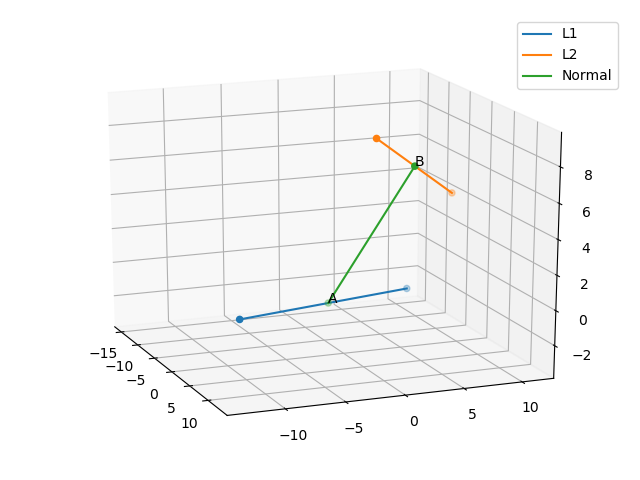
\includegraphics[width=\columnwidth]{12/11/2/15/figs/Figure_1.png}
\caption{}
\label{fig:12/11/2/15/}
\end{figure}


    \item Find the shortest distance between the lines whose vector equations are
    \begin{align}
        \vec{x} = \myvec{1\\2\\3} + \lambda_1\myvec{1\\-3\\2}
        \label{eq:12/11/2/16/L1}
    \end{align}
    and
    \begin{align}
        \vec{x} = \myvec{4\\5\\6} + \lambda_2\myvec{2\\3\\1}
        \label{eq:12/11/2/16/L2}
    \end{align}
    \solution
		\iffalse
\documentclass[journal,12pt,twocolumn]{IEEEtran}
\usepackage{setspace}
\usepackage{gensymb}
\usepackage{xcolor}
\usepackage{caption}
\singlespacing
\usepackage{siunitx}
\usepackage[cmex10]{amsmath}
\usepackage{mathtools}
\usepackage{hyperref}
\usepackage{amsthm}
\usepackage{mathrsfs}
\usepackage{txfonts}
\usepackage{stfloats}
\usepackage{cite}
\usepackage{cases}
\usepackage{subfig}
\usepackage{longtable}
\usepackage{multirow}
\usepackage{enumitem}
\usepackage{bm}
\usepackage{mathtools}
\usepackage{listings}
\usepackage{tikz}
\usetikzlibrary{shapes,arrows,positioning}
\usepackage{circuitikz}
\renewcommand{\vec}[1]{\boldsymbol{\mathbf{#1}}}
\DeclareMathOperator*{\Res}{Res}
\renewcommand\thesection{\arabic{section}}
\renewcommand\thesubsection{\thesection.\arabic{subsection}}
\renewcommand\thesubsubsection{\thesubsection.\arabic{subsubsection}}

\renewcommand\thesectiondis{\arabic{section}}
\renewcommand\thesubsectiondis{\thesectiondis.\arabic{subsection}}
\renewcommand\thesubsubsectiondis{\thesubsectiondis.\arabic{subsubsection}}
\hyphenation{op-tical net-works semi-conduc-tor}

\lstset{
language=Python,
frame=single, 
breaklines=true,
columns=fullflexible
}
\begin{document}
\theoremstyle{definition}
\newtheorem{theorem}{Theorem}[section]
\newtheorem{problem}{Problem}
\newtheorem{proposition}{Proposition}[section]
\newtheorem{lemma}{Lemma}[section]
\newtheorem{corollary}[theorem]{Corollary}
\newtheorem{example}{Example}[section]
\newtheorem{definition}{Definition}[section]
\newcommand{\BEQA}{\begin{eqnarray}}
\newcommand{\EEQA}{\end{eqnarray}}
\newcommand{\define}{\stackrel{\triangle}{=}}
\newcommand{\myvec}[1]{\ensuremath{\begin{pmatrix}#1\end{pmatrix}}}
\newcommand{\mydet}[1]{\ensuremath{\begin{vmatrix}#1\end{vmatrix}}}
\bibliographystyle{IEEEtran}
\providecommand{\nCr}[2]{\,^{#1}C_{#2}} % nCr
\providecommand{\nPr}[2]{\,^{#1}P_{#2}} % nPr
\providecommand{\mbf}{\mathbf}
\providecommand{\pr}[1]{\ensuremath{\Pr\left(#1\right)}}
\providecommand{\qfunc}[1]{\ensuremath{Q\left(#1\right)}}
\providecommand{\sbrak}[1]{\ensuremath{{}\left[#1\right]}}
\providecommand{\lsbrak}[1]{\ensuremath{{}\left[#1\right.}}
\providecommand{\rsbrak}[1]{\ensuremath{{}\left.#1\right]}}
\providecommand{\brak}[1]{\ensuremath{\left(#1\right)}}
\providecommand{\lbrak}[1]{\ensuremath{\left(#1\right.}}
\providecommand{\rbrak}[1]{\ensuremath{\left.#1\right)}}
\providecommand{\cbrak}[1]{\ensuremath{\left\{#1\right\}}}
\providecommand{\lcbrak}[1]{\ensuremath{\left\{#1\right.}}
\providecommand{\rcbrak}[1]{\ensuremath{\left.#1\right\}}}
\theoremstyle{remark}
\newtheorem{rem}{Remark}
\newcommand{\sgn}{\mathop{\mathrm{sgn}}}
\newcommand{\rect}{\mathop{\mathrm{rect}}}
\newcommand{\sinc}{\mathop{\mathrm{sinc}}}
\providecommand{\abs}[1]{\left\vert#1\right\vert}
\providecommand{\res}[1]{\Res\displaylimits_{#1}} 
\providecommand{\norm}[1]{\lVert#1\rVert}
\providecommand{\mtx}[1]{\mathbf{#1}}
\providecommand{\mean}[1]{E\left[ #1 \right]}
\providecommand{\fourier}{\overset{\mathcal{F}}{ \rightleftharpoons}}
\providecommand{\ztrans}{\overset{\mathcal{Z}}{ \rightleftharpoons}}
\providecommand{\system}[1]{\overset{\mathcal{#1}}{ \longleftrightarrow}}
\newcommand{\solution}{\noindent \textbf{Solution: }}
\providecommand{\dec}[2]{\ensuremath{\overset{#1}{\underset{#2}{\gtrless}}}}
\let\StandardTheFigure\thefigure
\def\putbox#1#2#3{\makebox[0in][l]{\makebox[#1][l]{}\raisebox{\baselineskip}[0in][0in]{\raisebox{#2}[0in][0in]{#3}}}}
     \def\rightbox#1{\makebox[0in][r]{#1}}
     \def\centbox#1{\makebox[0in]{#1}}
     \def\topbox#1{\raisebox{-\baselineskip}[0in][0in]{#1}}
     \def\midbox#1{\raisebox{-0.5\baselineskip}[0in][0in]{#1}}

\vspace{3cm}
\title{Line Assignment}
\author{Gautam Singh}
\maketitle
\bigskip

\begin{abstract}
    This document contains the solution to Question 16 of Exercise 2 in Chapter
    11 of the class 12 NCERT textbook.
\end{abstract}
\fi
    In this case,
    \begin{align}
        \vec{x_1} = \myvec{1\\2\\3} \quad \vec{x_2} = \myvec{4\\5\\6}
        \quad \vec{m_1} = \myvec{1\\-3\\2} \quad \vec{m_2} = \myvec{2\\3\\1}
        \label{eq:12/11/2/16/vals}
    \end{align}
    To check whether \eqref{eq:12/11/2/16/intersect-cond} has a solution in $\vec{\lambda}$,
    we use the augmented matrix.
    \begin{align}
        \myvec{1&2&3\\-3&3&3\\2&1&3} &\xleftrightarrow[]{R_2\leftarrow R_2+3R_1} \myvec{1&2&3\\0&9&12\\2&1&3} \\
                &\xleftrightarrow[]{R_3\leftarrow R_3-2R_1} \myvec{1&2&3\\0&9&12\\0&-3&-3} \\
                &\xleftrightarrow[]{R_3\leftarrow 3R_3+R_2} \myvec{1&2&3\\0&9&12\\0&0&3}
                \label{eq:12/11/2/16/rank-aug}
    \end{align}
    Clearly, the rank of this matrix is 3, and therefore, the lines are skew.
%
    Substituting from \eqref{eq:12/11/2/16/vals} in \eqref{eq:12/11/2/16/lambda-eqn} and forming the 
    augmented matrix,
    \begin{align}
        \myvec{14&-5&0\\-5&14&18} &\xleftrightarrow[]{R_1\leftarrow R_1+R_2} \myvec{9&9&18\\-5&14&18} \\
                 &\xleftrightarrow[]{R_1\leftarrow\frac{R_1}{9}} \myvec{1&1&2\\-5&14&18} \\
                 &\xleftrightarrow[]{R_2\leftarrow R_2+5R_1} \myvec{1&1&2\\0&19&28} \\
                 &\xleftrightarrow[]{R_1\leftarrow19R_1-R_2} \myvec{19&0&10\\0&19&28} \\
                 &\xleftrightarrow[]{\substack{R_1\leftarrow\frac{R_1}{19}\\R_2\leftarrow\frac{R_2}{9}}}
                    \myvec{1&0&\frac{10}{19}\\0&1&\frac{28}{19}} \\
                    \implies \vec{\lambda} &= \frac{1}{19}\myvec{10\\28}
        \label{eq:12/11/2/16/lambda-sol}
    \end{align}
    Hence, using \eqref{eq:12/11/2/16/lambda-def} and substituing into \eqref{eq:12/11/2/16/a-def} and \eqref{eq:12/11/2/16/b-def},
    \begin{align}
        \vec{A} = \frac{1}{19}\myvec{29\\8\\77} \quad \vec{B} = \frac{1}{19}\myvec{20\\11\\86}
    \end{align}
    Thus, the required distance is
    \begin{align}
        \norm{\vec{B}-\vec{A}} = \frac{\sqrt{9^2 +3^2 +(-9)^2}}{19} = \frac{3}{\sqrt{19}}
    \end{align}
    The situation is depicted in Fig. \ref{fig:12/11/2/16/skew}.

    \begin{figure}[!ht]
        \centering
        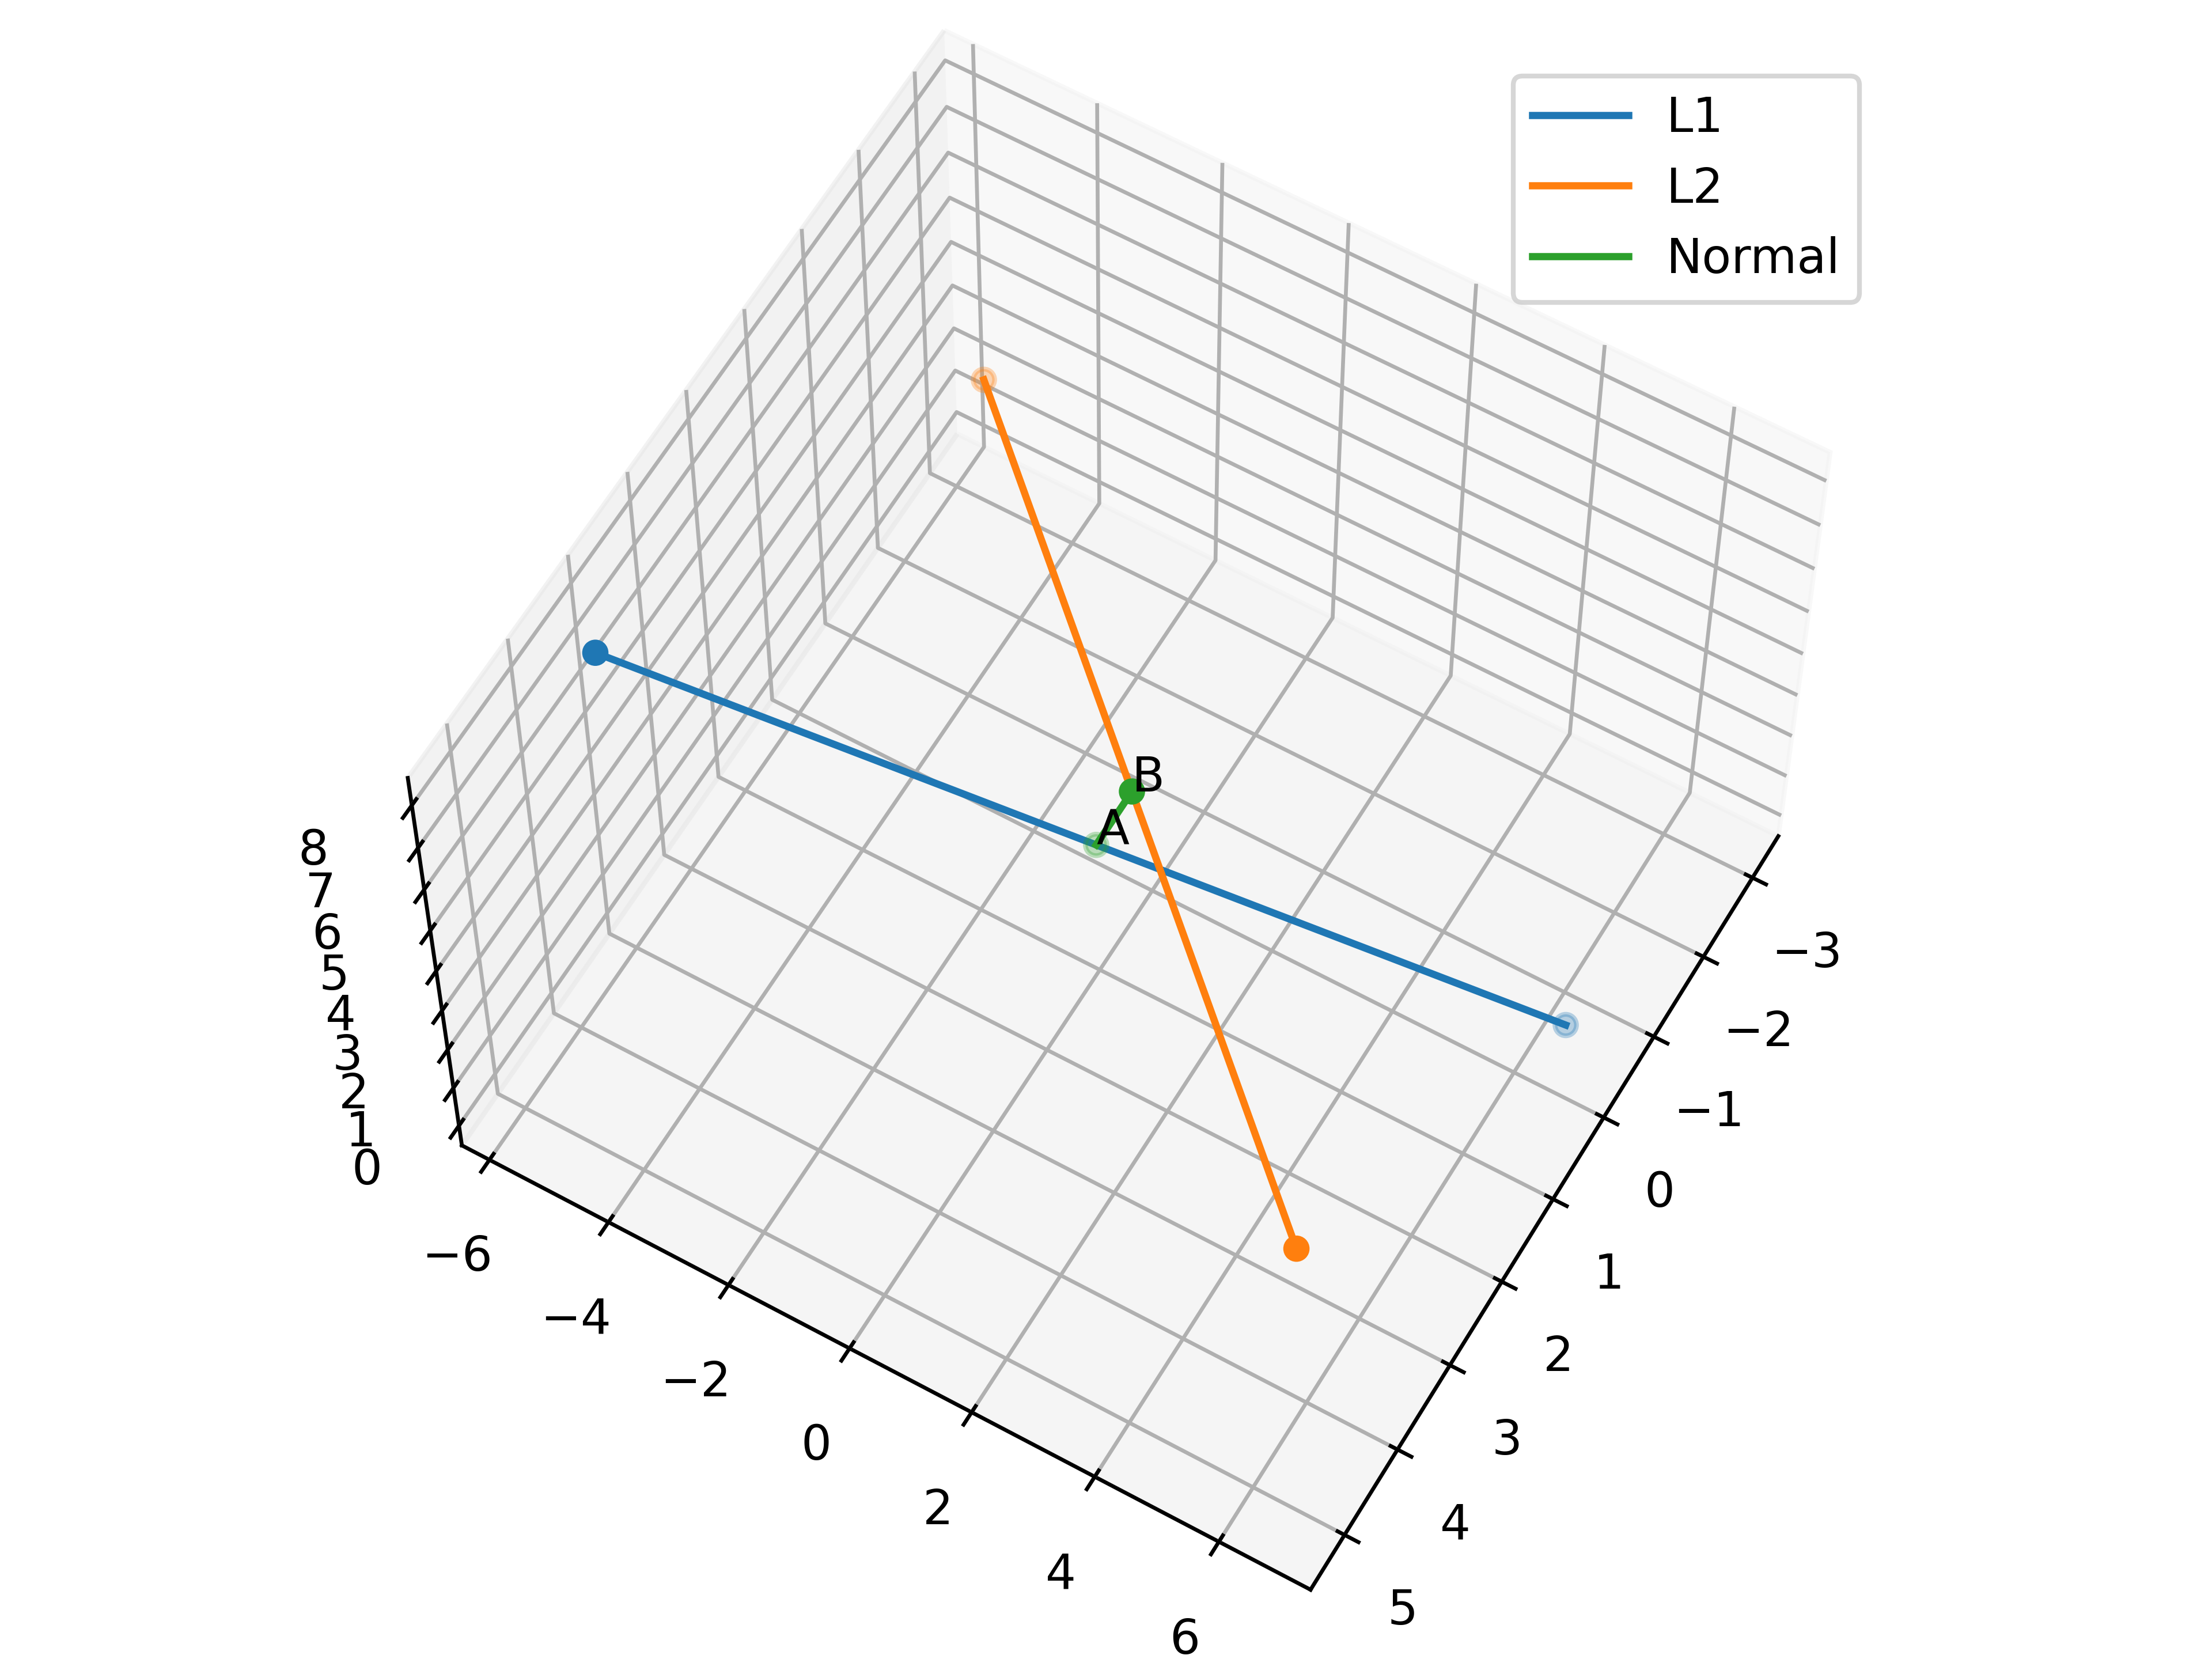
\includegraphics[width=\columnwidth]{12/11/2/16/figs/skew.png}
        \caption{$AB$ is the required shortest distance.}
        \label{fig:12/11/2/16/skew}
    \end{figure}

 \item 
\item Find the shortest distance between the lines $l_1$ and $l_2$ whose vector equations are ${\overrightarrow{r} = \hat{i}+\hat{j}+\lambda(2\hat{i}-\hat{j}+\hat{k})}$ and ${\overrightarrow{r} = 2\hat{i}+\hat{j}-\hat{k}+\mu(3\hat{i}-5\hat{j}+2\hat{k})}$.
    \solution
		\iffalse
\documentclass[journal,12pt,twocolumn]{IEEEtran}
\usepackage{romannum}
\usepackage{float}
\usepackage{setspace}
\usepackage{gensymb}
\singlespacing
\usepackage[cmex10]{amsmath}
\usepackage{amsthm}
\usepackage{mathrsfs}
\usepackage{txfonts}
\usepackage{stfloats}
\usepackage{bm}
\usepackage{cite}
\usepackage{cases}
\usepackage{subfig}
\usepackage{longtable}
\usepackage{multirow}
\usepackage{enumitem}
\usepackage{mathtools}
\usepackage{steinmetz}
\usepackage{tikz}
\usepackage{circuitikz}
\usepackage{verbatim}
\usepackage{tfrupee}
\usepackage[breaklinks=true]{hyperref}
\usepackage{tkz-euclide}
\usetikzlibrary{calc,math}
\usepackage{listings}
    \usepackage{color}                                            %%
    \usepackage{array}                                            %%
    \usepackage{longtable}                                        %%
    \usepackage{calc}                                             %%
    \usepackage{multirow}                                         %%
    \usepackage{hhline}                                           %%
    \usepackage{ifthen}                                           %%
  %optionally (for landscape tables embedded in another document): %%
    \usepackage{lscape}     
\usepackage{multicol}
\usepackage{chngcntr}
\DeclareMathOperator*{\Res}{Res}
\renewcommand\thesection{\arabic{section}}
\renewcommand\thesubsection{\thesection.\arabic{subsection}}
\renewcommand\thesubsubsection{\thesubsection.\arabic{subsubsection}}

\renewcommand\thesectiondis{\arabic{section}}
\renewcommand\thesubsectiondis{\thesectiondis.\arabic{subsection}}
\renewcommand\thesubsubsectiondis{\thesubsectiondis.\arabic{subsubsection}}

% correct bad hyphenation here
\hyphenation{op-tical net-works semi-conduc-tor}
\def\inputGnumericTable{}                                 %%

\lstset{
frame=single, 
breaklines=true,
columns=fullflexible
}

\begin{document}


\newtheorem{theorem}{Theorem}[section]
\newtheorem{problem}{Problem}
\newtheorem{proposition}{Proposition}[section]
\newtheorem{lemma}{Lemma}[section]
\newtheorem{corollary}[theorem]{Corollary}
\newtheorem{example}{Example}[section]
\newtheorem{definition}[problem]{Definition}
\newcommand{\BEQA}{\begin{eqnarray}}
\newcommand{\EEQA}{\end{eqnarray}}
\newcommand{\define}{\stackrel{\triangle}{=}}

\bibliographystyle{IEEEtran}
\providecommand{\mbf}{\mathbf}
\providecommand{\pr}[1]{\ensuremath{\Pr\left(#1\right)}}
\providecommand{\qfunc}[1]{\ensuremath{Q\left(#1\right)}}
\providecommand{\sbrak}[1]{\ensuremath{{}\left[#1\right]}}
\providecommand{\lsbrak}[1]{\ensuremath{{}\left[#1\right.}}
\providecommand{\rsbrak}[1]{\ensuremath{{}\left.#1\right]}}
\providecommand{\brak}[1]{\ensuremath{\left(#1\right)}}
\providecommand{\lbrak}[1]{\ensuremath{\left(#1\right.}}
\providecommand{\rbrak}[1]{\ensuremath{\left.#1\right)}}
\providecommand{\cbrak}[1]{\ensuremath{\left\{#1\right\}}}
\providecommand{\lcbrak}[1]{\ensuremath{\left\{#1\right.}}
\providecommand{\rcbrak}[1]{\ensuremath{\left.#1\right\}}}
\theoremstyle{remark}
\newtheorem{rem}{Remark}
\newcommand{\sgn}{\mathop{\mathrm{sgn}}}
\providecommand{\abs}[1]{\left\vert#1\right\vert}
\providecommand{\res}[1]{\Res\displaylimits_{#1}} 
\providecommand{\norm}[1]{\left\lVert#1\right\rVert}
\providecommand{\mtx}[1]{\mathbf{#1}}
\providecommand{\mean}[1]{E\left[ #1 \right]}
\providecommand{\fourier}{\overset{\mathcal{F}}{ \rightleftharpoons}}
\providecommand{\system}{\overset{\mathcal{H}}{ \longleftrightarrow}}
\newcommand{\solution}{\noindent \textbf{Solution: }}
\newcommand{\cosec}{\,\text{cosec}\,}
\providecommand{\dec}[2]{\ensuremath{\overset{#1}{\underset{#2}{\gtrless}}}}
\newcommand{\myvec}[1]{\ensuremath{\begin{pmatrix}#1\end{pmatrix}}}
\newcommand{\mydet}[1]{\ensuremath{\begin{vmatrix}#1\end{vmatrix}}}
\numberwithin{equation}{subsection}
\makeatletter
\@addtoreset{figure}{problem}
\makeatother

\let\StandardTheFigure\thefigure
\let\vec\mathbf
\renewcommand{\thefigure}{\theproblem}



\def\putbox#1#2#3{\makebox[0in][l]{\makebox[#1][l]{}\raisebox{\baselineskip}[0in][0in]{\raisebox{#2}[0in][0in]{#3}}}}
     \def\rightbox#1{\makebox[0in][r]{#1}}
     \def\centbox#1{\makebox[0in]{#1}}
     \def\topbox#1{\raisebox{-\baselineskip}[0in][0in]{#1}}
     \def\midbox#1{\raisebox{-0.5\baselineskip}[0in][0in]{#1}}

\vspace{3cm}


\title{Assignment 1}
\author{Jaswanth Chowdary Madala}





% make the title area
\maketitle

\newpage

%\tableofcontents

\bigskip

\renewcommand{\thefigure}{\theenumi}
\renewcommand{\thetable}{\theenumi}

\begin{enumerate}

\textbf{Solution:}
\fi
		The givne lines can be written  in vector form  as
\begin{align}
	\vec{x} &= \myvec{1\\1\\0} + \lambda_1\myvec{2\\-1\\1},
\vec{x} = \myvec{2\\1\\-1} + \lambda_2\myvec{3\\-5\\2}\\
\implies \vec{x_1} = \myvec{1\\1\\0},\, \vec{x_2} &= \myvec{2\\1\\-1}, \,\vec{m_1} = \myvec{2\\-1\\1}, \, \vec{m_2} = \myvec{3\\-5\\2}
\end{align}
%
We first check whether the given lines are skew. The lines 
\begin{align}
\vec{x} = \vec{x_1} + \lambda_1\vec{m_1},\, \vec{x} = \vec{x_2} + \lambda_2\vec{m_2} 
\label{eq:12/11/2/e11/1}
\end{align}
intersect if
\begin{align}
\vec{M}\bm{\lambda} &= \vec{x_2} - \vec{x_1}\\
\vec{M} &\triangleq \myvec{\vec{m_1} & \vec{m_2}} \\
\bm{\lambda} &\triangleq \myvec{\lambda_1\\-\lambda_2}\\
\end{align}
Here we have,
\begin{align}
\vec{M} &= \myvec{2&3\\-1&-5\\1&2},
\vec{x_2} - \vec{x_1} &= \myvec{1\\0\\-1}
\end{align}
We check whether the equation \eqref{eq:12/11/2/e11/2} has a solution
\begin{align}
\myvec{2&3\\-1&-5\\1&2}\bm{\lambda} = \myvec{1\\0\\-1}
\label{eq:12/11/2/e11/2}
\end{align}
The augmented matrix is given by,
\begin{align}
\myvec{2&3&\vrule&1\\-1&-5&\vrule&0\\1&2&\vrule&-1}
\xleftrightarrow[R_3 \leftarrow R_3 - \frac{1}{2}R_1]{R_2 \leftarrow R_2 + \frac{1}{2}R_1}
\myvec{2&3&\vrule&1\\&&\vrule\\0&-\frac{7}{2}&\vrule&\frac{1}{2}\\&&\vrule\\0&\frac{1}{2}&\vrule&-\frac{3}{2}}\\
\xleftrightarrow{R_3 \leftarrow R_3 + 7R_2}
\myvec{2&3&\vrule&1\\&&\vrule\\0&-\frac{7}{2}&\vrule&\frac{1}{2}\\&&\vrule\\0&0&\vrule&-10}
\end{align}
The rank of the matrix is 3. So the given lines are skew.
The closest points on two skew lines defined by \eqref{eq:12/11/2/e11/1} are given by 
\begin{align}
\vec{M}^\top \vec{M}\bm{\lambda} &= \vec{M}^\top\brak{\vec{x_2}-\vec{x_1}}\\
\implies \myvec{2&-1&1\\3&-5&2} \myvec{2&3\\-1&-5\\1&2}\bm{\lambda} &= \myvec{2&-1&1\\3&-5&2} \myvec{1\\0\\-1}\\
\implies \myvec{6&13\\13&38}\bm{\lambda} &= \myvec{1\\1}
\label{eq:12/11/2/e11/3}
\end{align}
The augmented matrix of the above equation \eqref{eq:12/11/2/e11/3} is given by,
\begin{align}
\myvec{6&13&\vrule&1\\13&38&\vrule&1}
\xleftrightarrow{R_2 \leftarrow R_2 - \frac{13}{6}R_1}
\myvec{6&13&\vrule&1 \\&&\vrule\\ 0&\frac{59}{6}&\vrule&-\frac{7}{6}}\\
\xleftrightarrow{R_1 \leftarrow R_1 - \frac{78}{59}R_2}
\myvec{6&0&\vrule&\frac{150}{59} \\&&\vrule\\ 0&\frac{59}{6}&\vrule&-\frac{7}{6}}
\end{align}
So, we get
\begin{align}
\myvec{\lambda_1\\-\lambda_2} &= \myvec{\frac{25}{59}\\\\-\frac{7}{59}}
\end{align}
The closest points $\vec{A}$ on line $l_1$ and $\vec{B}$ on line $l_2$ are given by,
\begin{align}
\vec{A} &= \vec{x_1} + \lambda_1\vec{m_1}
= \frac{1}{59}\myvec{109\\34\\25}\\
\vec{B} &= \vec{x_2} + \lambda_2\vec{m_2}
= \frac{1}{59}\myvec{139\\24\\-45}
\end{align}
The minimum distance between the lines is given by,
\begin{align}
\norm{\vec{B}-\vec{A}} &= \norm{\frac{1}{59}\myvec{30\\-10\\-70}}
= \frac{10}{\sqrt{59}}
\end{align}
See Fig. 
	\ref{fig:12/11/2/e11/}.
\begin{figure}[!ht]
\centering
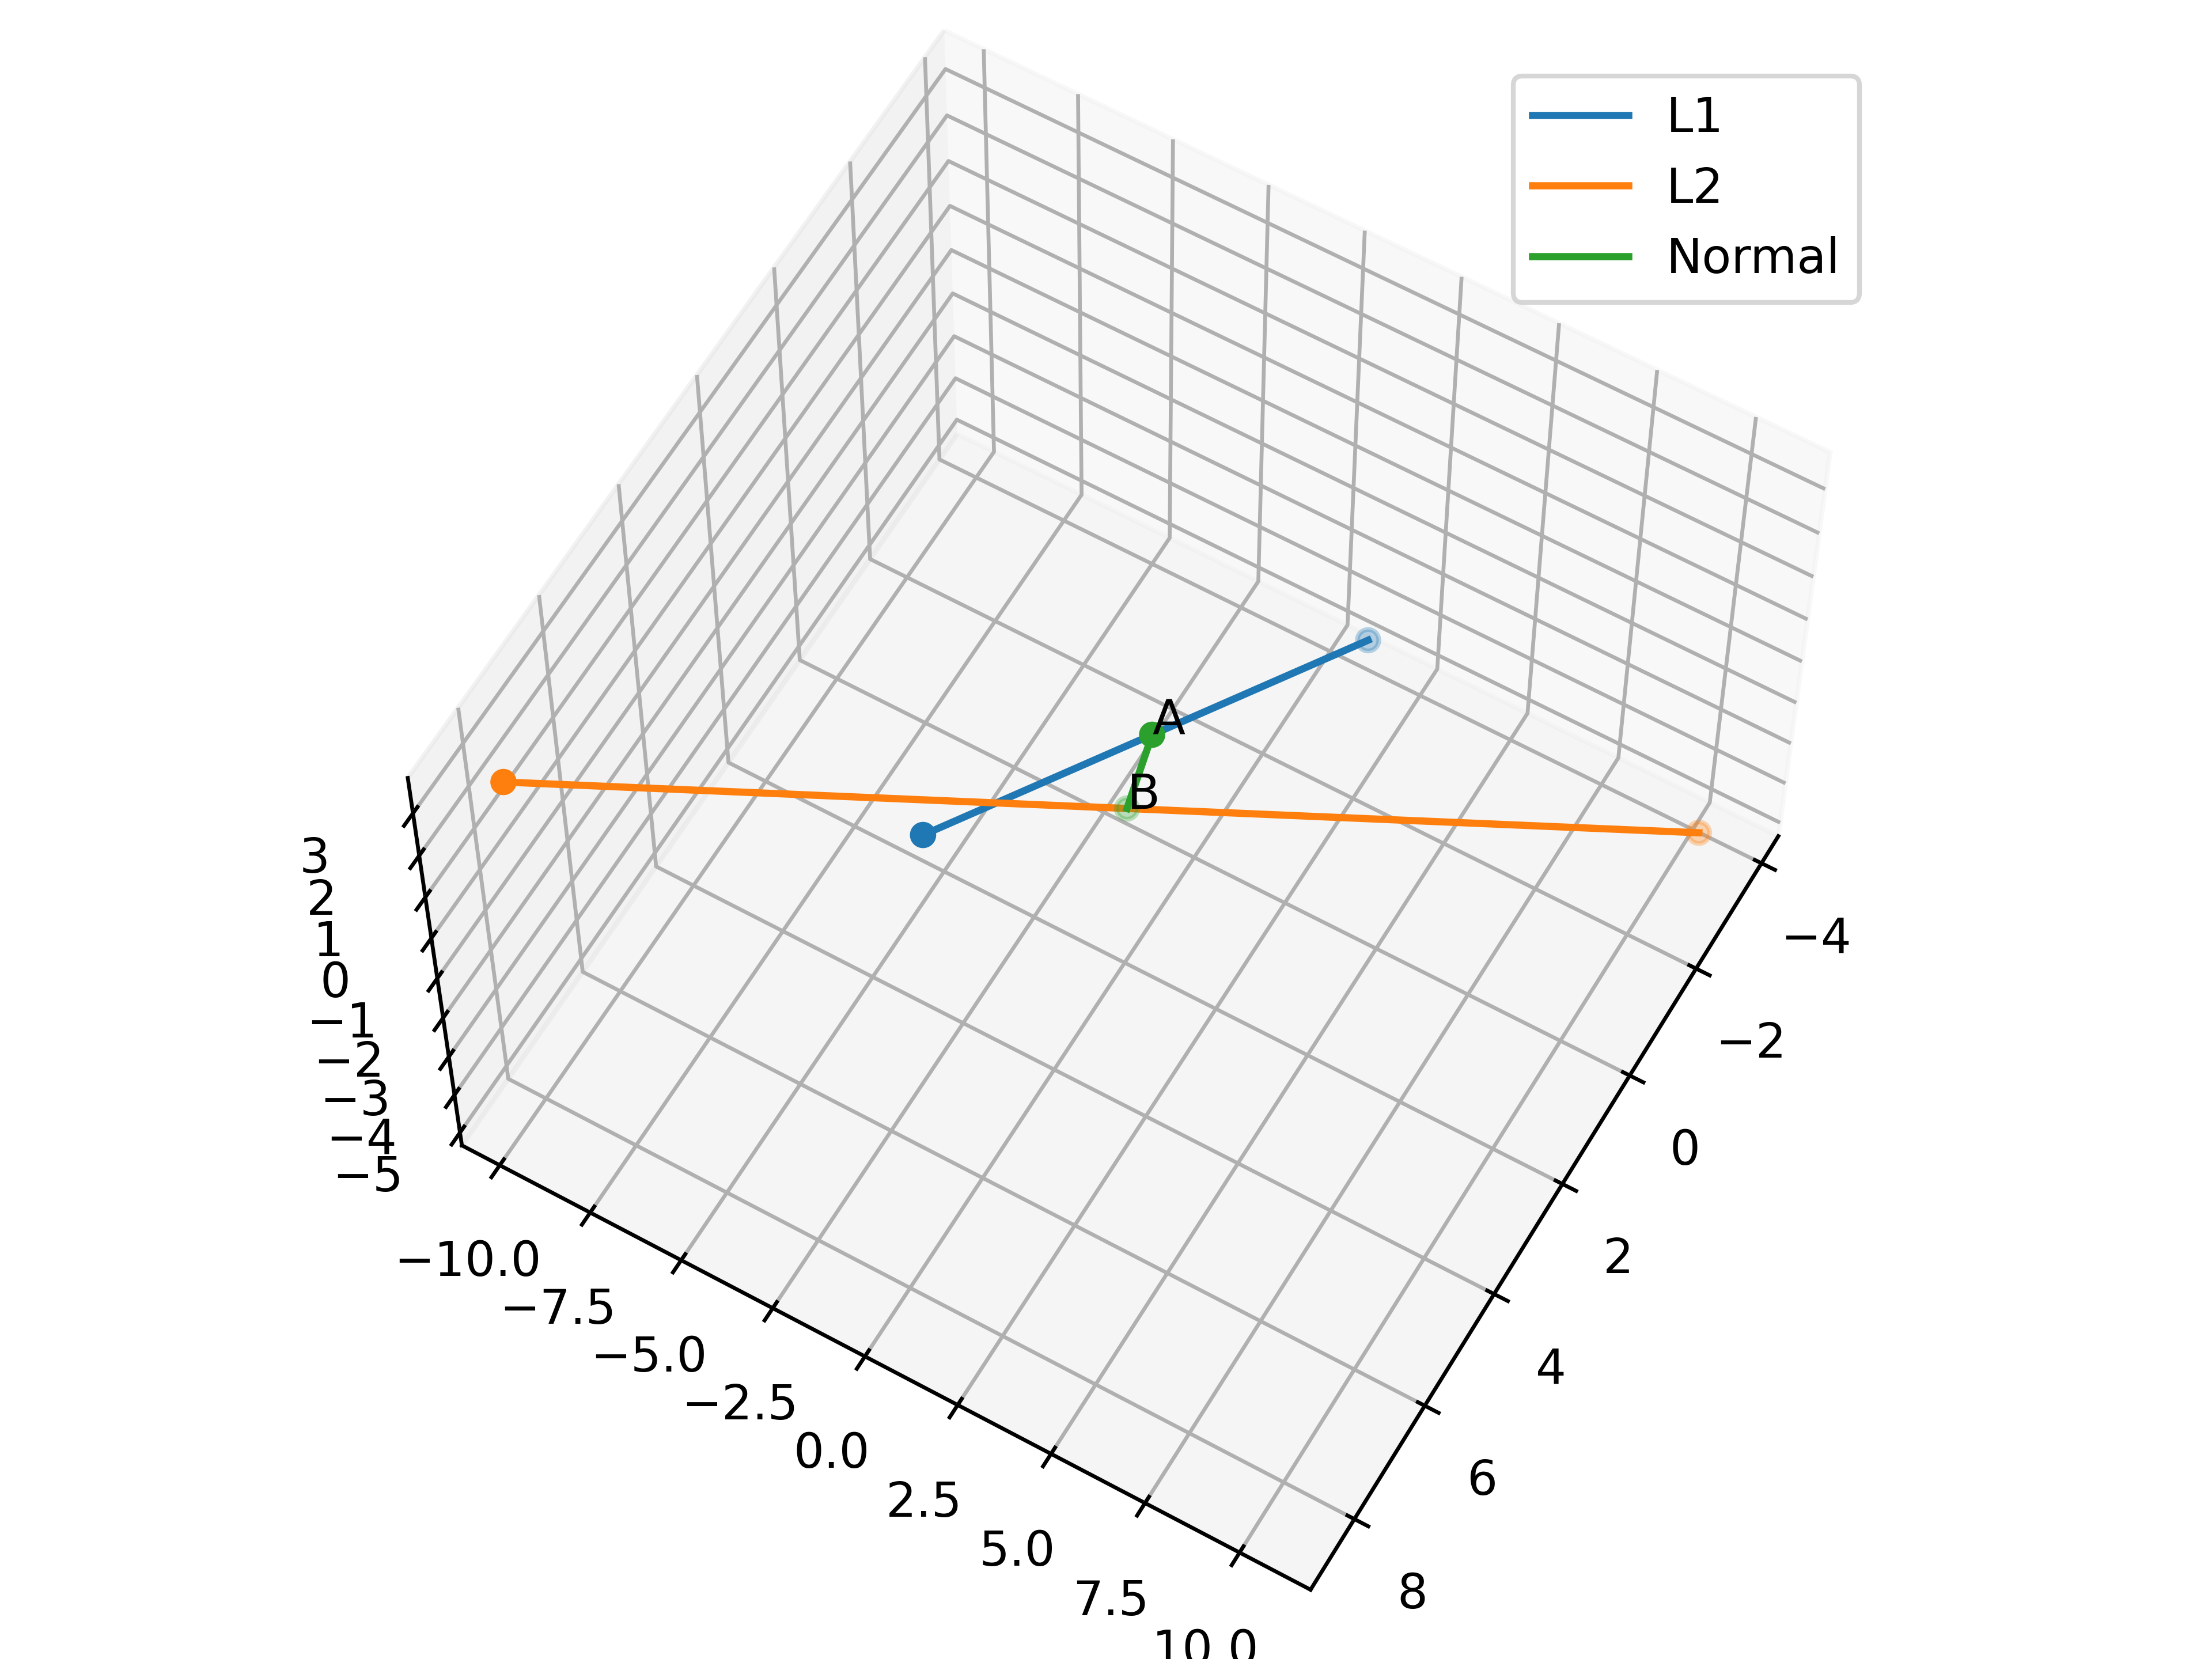
\includegraphics[width=\columnwidth]{12/11/2/e11/figs/skew.png}
\caption{}
	\label{fig:12/11/2/e11/}
\end{figure}

\end{enumerate}


\chapter{PT-100}
This chapter illustrates the modeling of the voltage-temperature 
characteristics of the PT-100 RTD (Resistance Temperature Detector) using the 
least squares method.

\section{Training Data}
The training data gathered by the PT-100 to train the Arduino is shown in Table
\ref{tab:train}.

\begin{table}[!ht]
    \centering
    %%%%%%%%%%%%%%%%%%%%%%%%%%%%%%%%%%%%%%%%%%%%%%%%%%%%%%%%%%%%%%%%%%%%%%
%%                                                                  %%
%%  This is the header of a LaTeX2e file exported from Gnumeric.    %%
%%                                                                  %%
%%  This file can be compiled as it stands or included in another   %%
%%  LaTeX document. The table is based on the longtable package so  %%
%%  the longtable options (headers, footers...) can be set in the   %%
%%  preamble section below (see PRAMBLE).                           %%
%%                                                                  %%
%%  To include the file in another, the following two lines must be %%
%%  in the including file:                                          %%
%%        \def\inputGnumericTable{}                                 %%
%%  at the beginning of the file and:                               %%
%%        \input{name-of-this-file.tex}                             %%
%%  where the table is to be placed. Note also that the including   %%
%%  file must use the following packages for the table to be        %%
%%  rendered correctly:                                             %%
%%    \usepackage[latin1]{inputenc}                                 %%
%%    \usepackage{color}                                            %%
%%    \usepackage{array}                                            %%
%%    \usepackage{longtable}                                        %%
%%    \usepackage{calc}                                             %%
%%    \usepackage{multirow}                                         %%
%%    \usepackage{hhline}                                           %%
%%    \usepackage{ifthen}                                           %%
%%  optionally (for landscape tables embedded in another document): %%
%%    \usepackage{lscape}                                           %%
%%                                                                  %%
%%%%%%%%%%%%%%%%%%%%%%%%%%%%%%%%%%%%%%%%%%%%%%%%%%%%%%%%%%%%%%%%%%%%%%



%%  This section checks if we are begin input into another file or  %%
%%  the file will be compiled alone. First use a macro taken from   %%
%%  the TeXbook ex 7.7 (suggestion of Han-Wen Nienhuys).            %%
\def\ifundefined#1{\expandafter\ifx\csname#1\endcsname\relax}


%%  Check for the \def token for inputed files. If it is not        %%
%%  defined, the file will be processed as a standalone and the     %%
%%  preamble will be used.                                          %%
\ifundefined{inputGnumericTable}

%%  We must be able to close or not the document at the end.        %%
	\def\gnumericTableEnd{\end{document}}


%%%%%%%%%%%%%%%%%%%%%%%%%%%%%%%%%%%%%%%%%%%%%%%%%%%%%%%%%%%%%%%%%%%%%%
%%                                                                  %%
%%  This is the PREAMBLE. Change these values to get the right      %%
%%  paper size and other niceties.                                  %%
%%                                                                  %%
%%%%%%%%%%%%%%%%%%%%%%%%%%%%%%%%%%%%%%%%%%%%%%%%%%%%%%%%%%%%%%%%%%%%%%

	\documentclass[12pt%
			  %,landscape%
                    ]{report}
       \usepackage[latin1]{inputenc}
       \usepackage{fullpage}
       \usepackage{color}
       \usepackage{array}
       \usepackage{longtable}
       \usepackage{calc}
       \usepackage{multirow}
       \usepackage{hhline}
       \usepackage{ifthen}

	\begin{document}


%%  End of the preamble for the standalone. The next section is for %%
%%  documents which are included into other LaTeX2e files.          %%
\else

%%  We are not a stand alone document. For a regular table, we will %%
%%  have no preamble and only define the closing to mean nothing.   %%
    \def\gnumericTableEnd{}

%%  If we want landscape mode in an embedded document, comment out  %%
%%  the line above and uncomment the two below. The table will      %%
%%  begin on a new page and run in landscape mode.                  %%
%       \def\gnumericTableEnd{\end{landscape}}
%       \begin{landscape}


%%  End of the else clause for this file being \input.              %%
\fi

%%%%%%%%%%%%%%%%%%%%%%%%%%%%%%%%%%%%%%%%%%%%%%%%%%%%%%%%%%%%%%%%%%%%%%
%%                                                                  %%
%%  The rest is the gnumeric table, except for the closing          %%
%%  statement. Changes below will alter the table's appearance.     %%
%%                                                                  %%
%%%%%%%%%%%%%%%%%%%%%%%%%%%%%%%%%%%%%%%%%%%%%%%%%%%%%%%%%%%%%%%%%%%%%%

\providecommand{\gnumericmathit}[1]{#1} 
%%  Uncomment the next line if you would like your numbers to be in %%
%%  italics if they are italizised in the gnumeric table.           %%
%\renewcommand{\gnumericmathit}[1]{\mathit{#1}}
\providecommand{\gnumericPB}[1]%
{\let\gnumericTemp=\\#1\let\\=\gnumericTemp\hspace{0pt}}
 \ifundefined{gnumericTableWidthDefined}
        \newlength{\gnumericTableWidth}
        \newlength{\gnumericTableWidthComplete}
        \newlength{\gnumericMultiRowLength}
        \global\def\gnumericTableWidthDefined{}
 \fi
%% The following setting protects this code from babel shorthands.  %%
 \ifthenelse{\isundefined{\languageshorthands}}{}{\languageshorthands{english}}
%%  The default table format retains the relative column widths of  %%
%%  gnumeric. They can easily be changed to c, r or l. In that case %%
%%  you may want to comment out the next line and uncomment the one %%
%%  thereafter                                                      %%
\providecommand\gnumbox{\makebox[0pt]}
%%\providecommand\gnumbox[1][]{\makebox}

%% to adjust positions in multirow situations                       %%
\setlength{\bigstrutjot}{\jot}
\setlength{\extrarowheight}{\doublerulesep}

%%  The \setlongtables command keeps column widths the same across  %%
%%  pages. Simply comment out next line for varying column widths.  %%
\setlongtables

\setlength\gnumericTableWidth{%
	101pt+%
	69pt+%
	67pt+%
0pt}
\def\gumericNumCols{3}
\setlength\gnumericTableWidthComplete{\gnumericTableWidth+%
         \tabcolsep*\gumericNumCols*2+\arrayrulewidth*\gumericNumCols}
\ifthenelse{\lengthtest{\gnumericTableWidthComplete > \linewidth}}%
         {\def\gnumericScale{1*\ratio{\linewidth-%
                        \tabcolsep*\gumericNumCols*2-%
                        \arrayrulewidth*\gumericNumCols}%
{\gnumericTableWidth}}}%
{\def\gnumericScale{1}}

%%%%%%%%%%%%%%%%%%%%%%%%%%%%%%%%%%%%%%%%%%%%%%%%%%%%%%%%%%%%%%%%%%%%%%
%%                                                                  %%
%% The following are the widths of the various columns. We are      %%
%% defining them here because then they are easier to change.       %%
%% Depending on the cell formats we may use them more than once.    %%
%%                                                                  %%
%%%%%%%%%%%%%%%%%%%%%%%%%%%%%%%%%%%%%%%%%%%%%%%%%%%%%%%%%%%%%%%%%%%%%%

\ifthenelse{\isundefined{\gnumericColA}}{\newlength{\gnumericColA}}{}\settowidth{\gnumericColA}{\begin{tabular}{@{}p{101pt*\gnumericScale}@{}}x\end{tabular}}
\ifthenelse{\isundefined{\gnumericColB}}{\newlength{\gnumericColB}}{}\settowidth{\gnumericColB}{\begin{tabular}{@{}p{69pt*\gnumericScale}@{}}x\end{tabular}}
\ifthenelse{\isundefined{\gnumericColC}}{\newlength{\gnumericColC}}{}\settowidth{\gnumericColC}{\begin{tabular}{@{}p{67pt*\gnumericScale}@{}}x\end{tabular}}

\begin{tabular}[c]{%
	b{\gnumericColA}%
	b{\gnumericColB}%
	b{\gnumericColC}%
	}

%%%%%%%%%%%%%%%%%%%%%%%%%%%%%%%%%%%%%%%%%%%%%%%%%%%%%%%%%%%%%%%%%%%%%%
%%  The longtable options. (Caption, headers... see Goosens, p.124) %%
%	\caption{The Table Caption.}             \\	%
% \hline	% Across the top of the table.
%%  The rest of these options are table rows which are placed on    %%
%%  the first, last or every page. Use \multicolumn if you want.    %%

%%  Header for the first page.                                      %%
%	\multicolumn{3}{c}{The First Header} \\ \hline 
%	\multicolumn{1}{c}{colTag}	%Column 1
%	&\multicolumn{1}{c}{colTag}	%Column 2
%	&\multicolumn{1}{c}{colTag}	\\ \hline %Last column
%	\endfirsthead

%%  The running header definition.                                  %%
%	\hline
%	\multicolumn{3}{l}{\ldots\small\slshape continued} \\ \hline
%	\multicolumn{1}{c}{colTag}	%Column 1
%	&\multicolumn{1}{c}{colTag}	%Column 2
%	&\multicolumn{1}{c}{colTag}	\\ \hline %Last column
%	\endhead

%%  The running footer definition.                                  %%
%	\hline
%	\multicolumn{3}{r}{\small\slshape continued\ldots} \\
%	\endfoot

%%  The ending footer definition.                                   %%
%	\multicolumn{3}{c}{That's all folks} \\ \hline 
%	\endlastfoot
%%%%%%%%%%%%%%%%%%%%%%%%%%%%%%%%%%%%%%%%%%%%%%%%%%%%%%%%%%%%%%%%%%%%%%

\hhline{|-|-~}
	 \multicolumn{1}{|p{\gnumericColA}|}%
     {\gnumericPB{\raggedright}\gnumbox[l]{\textbf{Temperature ($^{\circ}$C)}}}
	&\multicolumn{1}{p{\gnumericColB}|}%
	{\gnumericPB{\raggedright}\gnumbox[l]{\textbf{Voltage (V)}}}
	&
\\
\hhline{|--|~}
	 \multicolumn{1}{|p{\gnumericColA}|}%
	{\gnumericPB{\raggedleft}\gnumbox[r]{66}}
	&\multicolumn{1}{p{\gnumericColB}|}%
	{\gnumericPB{\raggedleft}\gnumbox[r]{1.85}}
	&
\\
\hhline{|--|~}
	 \multicolumn{1}{|p{\gnumericColA}|}%
	{\gnumericPB{\raggedleft}\gnumbox[r]{27}}
	&\multicolumn{1}{p{\gnumericColB}|}%
	{\gnumericPB{\raggedleft}\gnumbox[r]{1.76}}
	&
\\
\hhline{|--|~}
	 \multicolumn{1}{|p{\gnumericColA}|}%
	{\gnumericPB{\raggedleft}\gnumbox[r]{2}}
	&\multicolumn{1}{p{\gnumericColB}|}%
	{\gnumericPB{\raggedleft}\gnumbox[r]{1.66}}
	&
\\
\hhline{|--|~}
	 \multicolumn{1}{|p{\gnumericColA}|}%
	{\gnumericPB{\raggedleft}\gnumbox[r]{23}}
	&\multicolumn{1}{p{\gnumericColB}|}%
	{\gnumericPB{\raggedleft}\gnumbox[r]{1.72}}
	&
\\
\hhline{|--|~}
	 \multicolumn{1}{|p{\gnumericColA}|}%
	{\gnumericPB{\raggedleft}\gnumbox[r]{56}}
	&\multicolumn{1}{p{\gnumericColB}|}%
	{\gnumericPB{\raggedleft}\gnumbox[r]{1.82}}
	&
\\
\hhline{|--|~}
	 \multicolumn{1}{|p{\gnumericColA}|}%
	{\gnumericPB{\raggedleft}\gnumbox[r]{34}}
	&\multicolumn{1}{p{\gnumericColB}|}%
	{\gnumericPB{\raggedleft}\gnumbox[r]{1.76}}
	&
\\
\hhline{|--|~}
	 \multicolumn{1}{|p{\gnumericColA}|}%
	{\gnumericPB{\raggedleft}\gnumbox[r]{33}}
	&\multicolumn{1}{p{\gnumericColB}|}%
	{\gnumericPB{\raggedleft}\gnumbox[r]{1.75}}
	&
\\
\hhline{|--|~}
	 \multicolumn{1}{|p{\gnumericColA}|}%
	{\gnumericPB{\raggedleft}\gnumbox[r]{31}}
	&\multicolumn{1}{p{\gnumericColB}|}%
	{\gnumericPB{\raggedleft}\gnumbox[r]{1.74}}
	&
\\
\hhline{|-|-|~}
\end{tabular}

\ifthenelse{\isundefined{\languageshorthands}}{}{\languageshorthands{\languagename}}
\gnumericTableEnd

    \caption{Training data.}
    \label{tab:train}
\end{table}

The C++ source \texttt{codes/data.cpp} was used along with \textit{platformio}
to drive the Arduino. The effective schematic circuit diagram is shown in 
\autoref{fig:ckt}.

\begin{figure}[!ht]
    \centering
    \begin{circuitikz} \draw
        (0,0) to[battery1, l=$5\ V$, invert] (0,2)
        to[R, l^=$10\ \Omega$] (3,2) to[short, -o] (5,2);
        \draw (3,2) to[R, l^=$P\ \Omega$] (3,0)
        -- (0,0);
        \draw (3,0) to[short, -o] (5,0);
    \end{circuitikz}
    \caption{Schematic Circuit Diagram to Measure the Output of PT-100 ($P$).}
    \label{fig:ckt}
\end{figure}

\section{Model}

For the PT-100, we use the Callendar-Van Dusen equation
\begin{align}
    V(T) &= V(0)\brak{1+AT+BT^2} \\
    \implies c &= \vec{n}^\top\vec{x} \label{eq:model}
\end{align}
where
\begin{align}
    c = V(T),\ \vec{n} = V(0)\myvec{1\\A\\B},\ \vec{x} = \myvec{1\\T\\T^2}
    \label{eq:x-y-theta-def}
\end{align}

For multiple points, \eqref{eq:model} becomes
\begin{align}
    \vec{X}^\top\vec{n} = \vec{C}
    \label{eq:lsq-eqn}
\end{align}
where
\begin{align}
    \vec{X} &= \myvec{1&1&\ldots&1\\T_1&T_2&\ldots&T_n\\T_1^2&T_2^2&\ldots&T_n^2} \\
    \vec{C} &= \myvec{V\brak{T_1}\\V\brak{T_2}\\\vdots\\V\brak{T_n}}
\end{align}
and $\vec{n}$ is the unknown.

\section{Solution}
We approximate $\vec{n}$ by using the least sqaures method. The Python code 
\texttt{codes/lsq.py} solves for $\vec{n}$.

The calculated value of $\vec{n}$ is
\begin{align}
    \vec{n} = \myvec{1.6547\\3.199\times10^{-3}\\-3.9599\times10^{-6}}
    \label{eq:opt-theta}
\end{align}

The approximation is shown in Fig. \ref{fig:train}.
\begin{figure}[!ht]
    \centering
    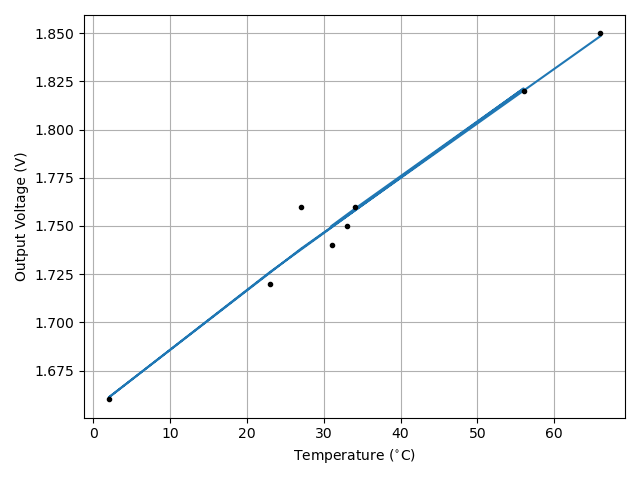
\includegraphics[width=\columnwidth]{pt100/figs/train.png}
    \caption{Training the model.}
    \label{fig:train}
\end{figure}

Thus, the approximate model is given by
\begin{align}
    V(T) &= 1.6547 + \brak{3.199\times10^{-3}}T \nonumber \\
         &- \brak{3.9599\times10^{-6}}T^2
    \label{eq:opt-model}
\end{align}

Notice in \eqref{eq:opt-model} that the coefficient of $T^2$ is negative, and 
hence the governing function is strictly concave. Hence, we cannot use gradient 
descent methods to solve this problem.

\section{Validation}
The validation dataset is shown in Table \ref{tab:valid}. The results of the 
validation are shown in Fig. \ref{fig:valid}.
\begin{table}[!ht]
    \centering
    %%%%%%%%%%%%%%%%%%%%%%%%%%%%%%%%%%%%%%%%%%%%%%%%%%%%%%%%%%%%%%%%%%%%%%
%%                                                                  %%
%%  This is the header of a LaTeX2e file exported from Gnumeric.    %%
%%                                                                  %%
%%  This file can be compiled as it stands or included in another   %%
%%  LaTeX document. The table is based on the longtable package so  %%
%%  the longtable options (headers, footers...) can be set in the   %%
%%  preamble section below (see PRAMBLE).                           %%
%%                                                                  %%
%%  To include the file in another, the following two lines must be %%
%%  in the including file:                                          %%
%%        \def\inputGnumericTable{}                                 %%
%%  at the beginning of the file and:                               %%
%%        \input{name-of-this-file.tex}                             %%
%%  where the table is to be placed. Note also that the including   %%
%%  file must use the following packages for the table to be        %%
%%  rendered correctly:                                             %%
%%    \usepackage[latin1]{inputenc}                                 %%
%%    \usepackage{color}                                            %%
%%    \usepackage{array}                                            %%
%%    \usepackage{longtable}                                        %%
%%    \usepackage{calc}                                             %%
%%    \usepackage{multirow}                                         %%
%%    \usepackage{hhline}                                           %%
%%    \usepackage{ifthen}                                           %%
%%  optionally (for landscape tables embedded in another document): %%
%%    \usepackage{lscape}                                           %%
%%                                                                  %%
%%%%%%%%%%%%%%%%%%%%%%%%%%%%%%%%%%%%%%%%%%%%%%%%%%%%%%%%%%%%%%%%%%%%%%



%%  This section checks if we are begin input into another file or  %%
%%  the file will be compiled alone. First use a macro taken from   %%
%%  the TeXbook ex 7.7 (suggestion of Han-Wen Nienhuys).            %%
\def\ifundefined#1{\expandafter\ifx\csname#1\endcsname\relax}


%%  Check for the \def token for inputed files. If it is not        %%
%%  defined, the file will be processed as a standalone and the     %%
%%  preamble will be used.                                          %%
\ifundefined{inputGnumericTable}

%%  We must be able to close or not the document at the end.        %%
	\def\gnumericTableEnd{\end{document}}


%%%%%%%%%%%%%%%%%%%%%%%%%%%%%%%%%%%%%%%%%%%%%%%%%%%%%%%%%%%%%%%%%%%%%%
%%                                                                  %%
%%  This is the PREAMBLE. Change these values to get the right      %%
%%  paper size and other niceties.                                  %%
%%                                                                  %%
%%%%%%%%%%%%%%%%%%%%%%%%%%%%%%%%%%%%%%%%%%%%%%%%%%%%%%%%%%%%%%%%%%%%%%

	\documentclass[12pt%
			  %,landscape%
                    ]{report}
       \usepackage[latin1]{inputenc}
       \usepackage{fullpage}
       \usepackage{color}
       \usepackage{array}
       \usepackage{longtable}
       \usepackage{calc}
       \usepackage{multirow}
       \usepackage{hhline}
       \usepackage{ifthen}

	\begin{document}


%%  End of the preamble for the standalone. The next section is for %%
%%  documents which are included into other LaTeX2e files.          %%
\else

%%  We are not a stand alone document. For a regular table, we will %%
%%  have no preamble and only define the closing to mean nothing.   %%
    \def\gnumericTableEnd{}

%%  If we want landscape mode in an embedded document, comment out  %%
%%  the line above and uncomment the two below. The table will      %%
%%  begin on a new page and run in landscape mode.                  %%
%       \def\gnumericTableEnd{\end{landscape}}
%       \begin{landscape}


%%  End of the else clause for this file being \input.              %%
\fi

%%%%%%%%%%%%%%%%%%%%%%%%%%%%%%%%%%%%%%%%%%%%%%%%%%%%%%%%%%%%%%%%%%%%%%
%%                                                                  %%
%%  The rest is the gnumeric table, except for the closing          %%
%%  statement. Changes below will alter the table's appearance.     %%
%%                                                                  %%
%%%%%%%%%%%%%%%%%%%%%%%%%%%%%%%%%%%%%%%%%%%%%%%%%%%%%%%%%%%%%%%%%%%%%%

\providecommand{\gnumericmathit}[1]{#1} 
%%  Uncomment the next line if you would like your numbers to be in %%
%%  italics if they are italizised in the gnumeric table.           %%
%\renewcommand{\gnumericmathit}[1]{\mathit{#1}}
\providecommand{\gnumericPB}[1]%
{\let\gnumericTemp=\\#1\let\\=\gnumericTemp\hspace{0pt}}
 \ifundefined{gnumericTableWidthDefined}
        \newlength{\gnumericTableWidth}
        \newlength{\gnumericTableWidthComplete}
        \newlength{\gnumericMultiRowLength}
        \global\def\gnumericTableWidthDefined{}
 \fi
%% The following setting protects this code from babel shorthands.  %%
 \ifthenelse{\isundefined{\languageshorthands}}{}{\languageshorthands{english}}
%%  The default table format retains the relative column widths of  %%
%%  gnumeric. They can easily be changed to c, r or l. In that case %%
%%  you may want to comment out the next line and uncomment the one %%
%%  thereafter                                                      %%
\providecommand\gnumbox{\makebox[0pt]}
%%\providecommand\gnumbox[1][]{\makebox}

%% to adjust positions in multirow situations                       %%
\setlength{\bigstrutjot}{\jot}
\setlength{\extrarowheight}{\doublerulesep}

%%  The \setlongtables command keeps column widths the same across  %%
%%  pages. Simply comment out next line for varying column widths.  %%
\setlongtables

\setlength\gnumericTableWidth{%
	101pt+%
	69pt+%
	67pt+%
0pt}
\def\gumericNumCols{3}
\setlength\gnumericTableWidthComplete{\gnumericTableWidth+%
         \tabcolsep*\gumericNumCols*2+\arrayrulewidth*\gumericNumCols}
\ifthenelse{\lengthtest{\gnumericTableWidthComplete > \linewidth}}%
         {\def\gnumericScale{1*\ratio{\linewidth-%
                        \tabcolsep*\gumericNumCols*2-%
                        \arrayrulewidth*\gumericNumCols}%
{\gnumericTableWidth}}}%
{\def\gnumericScale{1}}

%%%%%%%%%%%%%%%%%%%%%%%%%%%%%%%%%%%%%%%%%%%%%%%%%%%%%%%%%%%%%%%%%%%%%%
%%                                                                  %%
%% The following are the widths of the various columns. We are      %%
%% defining them here because then they are easier to change.       %%
%% Depending on the cell formats we may use them more than once.    %%
%%                                                                  %%
%%%%%%%%%%%%%%%%%%%%%%%%%%%%%%%%%%%%%%%%%%%%%%%%%%%%%%%%%%%%%%%%%%%%%%

\ifthenelse{\isundefined{\gnumericColA}}{\newlength{\gnumericColA}}{}\settowidth{\gnumericColA}{\begin{tabular}{@{}p{101pt*\gnumericScale}@{}}x\end{tabular}}
\ifthenelse{\isundefined{\gnumericColB}}{\newlength{\gnumericColB}}{}\settowidth{\gnumericColB}{\begin{tabular}{@{}p{69pt*\gnumericScale}@{}}x\end{tabular}}
\ifthenelse{\isundefined{\gnumericColC}}{\newlength{\gnumericColC}}{}\settowidth{\gnumericColC}{\begin{tabular}{@{}p{67pt*\gnumericScale}@{}}x\end{tabular}}

\begin{tabular}[c]{%
	b{\gnumericColA}%
	b{\gnumericColB}%
	b{\gnumericColC}%
	}

%%%%%%%%%%%%%%%%%%%%%%%%%%%%%%%%%%%%%%%%%%%%%%%%%%%%%%%%%%%%%%%%%%%%%%
%%  The longtable options. (Caption, headers... see Goosens, p.124) %%
%	\caption{The Table Caption.}             \\	%
% \hline	% Across the top of the table.
%%  The rest of these options are table rows which are placed on    %%
%%  the first, last or every page. Use \multicolumn if you want.    %%

%%  Header for the first page.                                      %%
%	\multicolumn{3}{c}{The First Header} \\ \hline 
%	\multicolumn{1}{c}{colTag}	%Column 1
%	&\multicolumn{1}{c}{colTag}	%Column 2
%	&\multicolumn{1}{c}{colTag}	\\ \hline %Last column
%	\endfirsthead

%%  The running header definition.                                  %%
%	\hline
%	\multicolumn{3}{l}{\ldots\small\slshape continued} \\ \hline
%	\multicolumn{1}{c}{colTag}	%Column 1
%	&\multicolumn{1}{c}{colTag}	%Column 2
%	&\multicolumn{1}{c}{colTag}	\\ \hline %Last column
%	\endhead

%%  The running footer definition.                                  %%
%	\hline
%	\multicolumn{3}{r}{\small\slshape continued\ldots} \\
%	\endfoot

%%  The ending footer definition.                                   %%
%	\multicolumn{3}{c}{That's all folks} \\ \hline 
%	\endlastfoot
%%%%%%%%%%%%%%%%%%%%%%%%%%%%%%%%%%%%%%%%%%%%%%%%%%%%%%%%%%%%%%%%%%%%%%

\hhline{|-|-~}
	 \multicolumn{1}{|p{\gnumericColA}|}%
     {\gnumericPB{\raggedright}\gnumbox[l]{\textbf{Temperature ($^{\circ}$C)}}}
	&\multicolumn{1}{p{\gnumericColB}|}%
	{\gnumericPB{\raggedright}\gnumbox[l]{\textbf{Voltage (V)}}}
	&
\\
\hhline{|--|~}
	 \multicolumn{1}{|p{\gnumericColA}|}%
	{\gnumericPB{\raggedleft}\gnumbox[r]{4}}
	&\multicolumn{1}{p{\gnumericColB}|}%
	{\gnumericPB{\raggedleft}\gnumbox[r]{1.67}}
	&
\\
\hhline{|--|~}
	 \multicolumn{1}{|p{\gnumericColA}|}%
	{\gnumericPB{\raggedleft}\gnumbox[r]{25}}
	&\multicolumn{1}{p{\gnumericColB}|}%
	{\gnumericPB{\raggedleft}\gnumbox[r]{1.73}}
	&
\\
\hhline{|--|~}
	 \multicolumn{1}{|p{\gnumericColA}|}%
	{\gnumericPB{\raggedleft}\gnumbox[r]{61}}
	&\multicolumn{1}{p{\gnumericColB}|}%
	{\gnumericPB{\raggedleft}\gnumbox[r]{1.83}}
	&
\\
\hhline{|--|~}
	 \multicolumn{1}{|p{\gnumericColA}|}%
	{\gnumericPB{\raggedleft}\gnumbox[r]{35}}
	&\multicolumn{1}{p{\gnumericColB}|}%
	{\gnumericPB{\raggedleft}\gnumbox[r]{1.77}}
	&
\\
\hhline{|-|-|~}
\end{tabular}

\ifthenelse{\isundefined{\languageshorthands}}{}{\languageshorthands{\languagename}}
\gnumericTableEnd

    \caption{Validation data.}
    \label{tab:valid}
\end{table}
\begin{figure}[!ht]
    \centering
    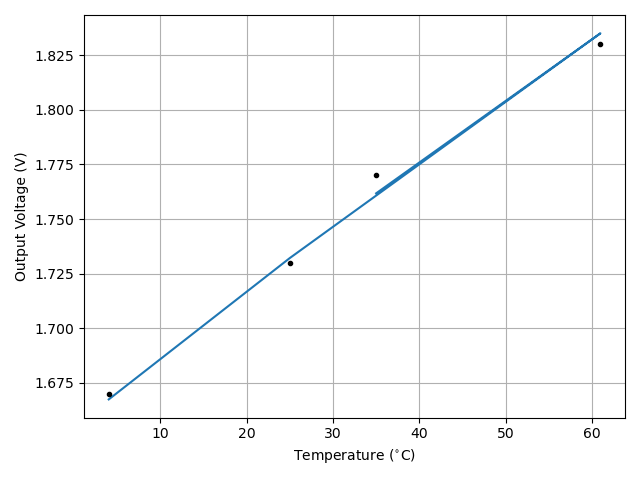
\includegraphics[width=\columnwidth]{pt100/figs/valid.png}
    \caption{Validating the model.}
    \label{fig:valid}
\end{figure}

\chapter{K-Means Method}
\section{Introduction}

We test the utility of the $K$-means algorithm in assigning grades
as compared to estimating the grades using the standard normal 
distribution. We consider the scores of $N = 94$ students who have taken 
a course in the  Indian Institute of Technology, Hyderabad (IITH) as our 
dataset.

\section{Fitting a Gaussian Curve}
Since $N$ is not very large, given the scores of each student 
$x_i,\ 1 \le i \le N$, we can compute the population mean and population 
variance as

\begin{align}
    \mu &= \mean{x} \\
    \sigma^2 &= \mean{\brak{x-\mu}^2}
    \label{eq:pop-param}
\end{align}

We assume that the scores $x \sim N\brak{\mu,\sigma^2}$. Thus, we compute the
$Z$-scores as
\begin{align}
    Z = \frac{x-\mu}{\sigma}
\end{align}

The grades are assigned as per Table \ref{tab:grade-scheme}.
\begin{table}[!ht]
    \centering
    %%%%%%%%%%%%%%%%%%%%%%%%%%%%%%%%%%%%%%%%%%%%%%%%%%%%%%%%%%%%%%%%%%%%%%
%%                                                                  %%
%%  This is the header of a LaTeX2e file exported from Gnumeric.    %%
%%                                                                  %%
%%  This file can be compiled as it stands or included in another   %%
%%  LaTeX document. The table is based on the longtable package so  %%
%%  the longtable options (headers, footers...) can be set in the   %%
%%  preamble section below (see PRAMBLE).                           %%
%%                                                                  %%
%%  To include the file in another, the following two lines must be %%
%%  in the including file:                                          %%
%%        \def\inputGnumericTable{}                                 %%
%%  at the beginning of the file and:                               %%
%%        \input{name-of-this-file.tex}                             %%
%%  where the table is to be placed. Note also that the including   %%
%%  file must use the following packages for the table to be        %%
%%  rendered correctly:                                             %%
%%    \usepackage[latin1]{inputenc}                                 %%
%%    \usepackage{color}                                            %%
%%    \usepackage{array}                                            %%
%%    \usepackage{longtable}                                        %%
%%    \usepackage{calc}                                             %%
%%    \usepackage{multirow}                                         %%
%%    \usepackage{hhline}                                           %%
%%    \usepackage{ifthen}                                           %%
%%  optionally (for landscape tables embedded in another document): %%
%%    \usepackage{lscape}                                           %%
%%                                                                  %%
%%%%%%%%%%%%%%%%%%%%%%%%%%%%%%%%%%%%%%%%%%%%%%%%%%%%%%%%%%%%%%%%%%%%%%



%%  This section checks if we are begin input into another file or  %%
%%  the file will be compiled alone. First use a macro taken from   %%
%%  the TeXbook ex 7.7 (suggestion of Han-Wen Nienhuys).            %%
\def\ifundefined#1{\expandafter\ifx\csname#1\endcsname\relax}


%%  Check for the \def token for inputed files. If it is not        %%
%%  defined, the file will be processed as a standalone and the     %%
%%  preamble will be used.                                          %%
\ifundefined{inputGnumericTable}

%%  We must be able to close or not the document at the end.        %%
	\def\gnumericTableEnd{\end{document}}


%%%%%%%%%%%%%%%%%%%%%%%%%%%%%%%%%%%%%%%%%%%%%%%%%%%%%%%%%%%%%%%%%%%%%%
%%                                                                  %%
%%  This is the PREAMBLE. Change these values to get the right      %%
%%  paper size and other niceties.                                  %%
%%                                                                  %%
%%%%%%%%%%%%%%%%%%%%%%%%%%%%%%%%%%%%%%%%%%%%%%%%%%%%%%%%%%%%%%%%%%%%%%

	\documentclass[12pt%
			  %,landscape%
                    ]{report}
       \usepackage[latin1]{inputenc}
       \usepackage{fullpage}
       \usepackage{color}
       \usepackage{array}
       \usepackage{longtable}
       \usepackage{calc}
       \usepackage{multirow}
       \usepackage{hhline}
       \usepackage{ifthen}

	\begin{document}


%%  End of the preamble for the standalone. The next section is for %%
%%  documents which are included into other LaTeX2e files.          %%
\else

%%  We are not a stand alone document. For a regular table, we will %%
%%  have no preamble and only define the closing to mean nothing.   %%
    \def\gnumericTableEnd{}

%%  If we want landscape mode in an embedded document, comment out  %%
%%  the line above and uncomment the two below. The table will      %%
%%  begin on a new page and run in landscape mode.                  %%
%       \def\gnumericTableEnd{\end{landscape}}
%       \begin{landscape}


%%  End of the else clause for this file being \input.              %%
\fi

%%%%%%%%%%%%%%%%%%%%%%%%%%%%%%%%%%%%%%%%%%%%%%%%%%%%%%%%%%%%%%%%%%%%%%
%%                                                                  %%
%%  The rest is the gnumeric table, except for the closing          %%
%%  statement. Changes below will alter the table's appearance.     %%
%%                                                                  %%
%%%%%%%%%%%%%%%%%%%%%%%%%%%%%%%%%%%%%%%%%%%%%%%%%%%%%%%%%%%%%%%%%%%%%%

\providecommand{\gnumericmathit}[1]{#1} 
%%  Uncomment the next line if you would like your numbers to be in %%
%%  italics if they are italizised in the gnumeric table.           %%
%\renewcommand{\gnumericmathit}[1]{\mathit{#1}}
\providecommand{\gnumericPB}[1]%
{\let\gnumericTemp=\\#1\let\\=\gnumericTemp\hspace{0pt}}
 \ifundefined{gnumericTableWidthDefined}
        \newlength{\gnumericTableWidth}
        \newlength{\gnumericTableWidthComplete}
        \newlength{\gnumericMultiRowLength}
        \global\def\gnumericTableWidthDefined{}
 \fi
%% The following setting protects this code from babel shorthands.  %%
 \ifthenelse{\isundefined{\languageshorthands}}{}{\languageshorthands{english}}
%%  The default table format retains the relative column widths of  %%
%%  gnumeric. They can easily be changed to c, r or l. In that case %%
%%  you may want to comment out the next line and uncomment the one %%
%%  thereafter                                                      %%
\providecommand\gnumbox{\makebox[0pt]}
%%\providecommand\gnumbox[1][]{\makebox}

%% to adjust positions in multirow situations                       %%
\setlength{\bigstrutjot}{\jot}
\setlength{\extrarowheight}{\doublerulesep}

%%  The \setlongtables command keeps column widths the same across  %%
%%  pages. Simply comment out next line for varying column widths.  %%
\setlongtables

\setlength\gnumericTableWidth{%
	53pt+%
	53pt+%
0pt}
\def\gumericNumCols{2}
\setlength\gnumericTableWidthComplete{\gnumericTableWidth+%
         \tabcolsep*\gumericNumCols*2+\arrayrulewidth*\gumericNumCols}
\ifthenelse{\lengthtest{\gnumericTableWidthComplete > \linewidth}}%
         {\def\gnumericScale{\ratio{\linewidth-%
                        \tabcolsep*\gumericNumCols*2-%
                        \arrayrulewidth*\gumericNumCols}%
{\gnumericTableWidth}}}%
{\def\gnumericScale{1}}

%%%%%%%%%%%%%%%%%%%%%%%%%%%%%%%%%%%%%%%%%%%%%%%%%%%%%%%%%%%%%%%%%%%%%%
%%                                                                  %%
%% The following are the widths of the various columns. We are      %%
%% defining them here because then they are easier to change.       %%
%% Depending on the cell formats we may use them more than once.    %%
%%                                                                  %%
%%%%%%%%%%%%%%%%%%%%%%%%%%%%%%%%%%%%%%%%%%%%%%%%%%%%%%%%%%%%%%%%%%%%%%

\ifthenelse{\isundefined{\gnumericColA}}{\newlength{\gnumericColA}}{}\settowidth{\gnumericColA}{\begin{tabular}{@{}p{53pt*\gnumericScale}@{}}x\end{tabular}}
\ifthenelse{\isundefined{\gnumericColB}}{\newlength{\gnumericColB}}{}\settowidth{\gnumericColB}{\begin{tabular}{@{}p{53pt*\gnumericScale}@{}}x\end{tabular}}

\begin{tabular}[c]{%
	b{\gnumericColA}%
	b{\gnumericColB}%
	}

%%%%%%%%%%%%%%%%%%%%%%%%%%%%%%%%%%%%%%%%%%%%%%%%%%%%%%%%%%%%%%%%%%%%%%
%%  The longtable options. (Caption, headers... see Goosens, p.124) %%
%	\caption{The Table Caption.}             \\	%
% \hline	% Across the top of the table.
%%  The rest of these options are table rows which are placed on    %%
%%  the first, last or every page. Use \multicolumn if you want.    %%

%%  Header for the first page.                                      %%
%	\multicolumn{2}{c}{The First Header} \\ \hline 
%	\multicolumn{1}{c}{colTag}	%Column 1
%	&\multicolumn{1}{c}{colTag}	\\ \hline %Last column
%	\endfirsthead

%%  The running header definition.                                  %%
%	\hline
%	\multicolumn{2}{l}{\ldots\small\slshape continued} \\ \hline
%	\multicolumn{1}{c}{colTag}	%Column 1
%	&\multicolumn{1}{c}{colTag}	\\ \hline %Last column
%	\endhead

%%  The running footer definition.                                  %%
%	\hline
%	\multicolumn{2}{r}{\small\slshape continued\ldots} \\
%	\endfoot

%%  The ending footer definition.                                   %%
%	\multicolumn{2}{c}{That's all folks} \\ \hline 
%	\endlastfoot
%%%%%%%%%%%%%%%%%%%%%%%%%%%%%%%%%%%%%%%%%%%%%%%%%%%%%%%%%%%%%%%%%%%%%%

\hhline{|-|-}
	 \multicolumn{1}{|p{\gnumericColA}|}%
	{\gnumericPB{\raggedright}\gnumbox[l]{\textbf{Interval}}}
	&\multicolumn{1}{p{\gnumericColB}|}%
	{\gnumericPB{\raggedright}\gnumbox[l]{\textbf{Grade}}}
\\
\hhline{|--|}
	 \multicolumn{1}{|p{\gnumericColA}|}%
	{\gnumericPB{\raggedright}\gnumbox[l]{($-\infty$, -3]}}
	&\multicolumn{1}{p{\gnumericColB}|}%
	{\gnumericPB{\raggedright}\gnumbox[l]{F}}
\\
\hhline{|--|}
	 \multicolumn{1}{|p{\gnumericColA}|}%
	{\gnumericPB{\raggedright}\gnumbox[l]{(-3, -2]}}
	&\multicolumn{1}{p{\gnumericColB}|}%
	{\gnumericPB{\raggedright}\gnumbox[l]{D}}
\\
\hhline{|--|}
	 \multicolumn{1}{|p{\gnumericColA}|}%
	{\gnumericPB{\raggedright}\gnumbox[l]{(-2, 1]}}
	&\multicolumn{1}{p{\gnumericColB}|}%
	{\gnumericPB{\raggedright}\gnumbox[l]{C}}
\\
\hhline{|--|}
	 \multicolumn{1}{|p{\gnumericColA}|}%
	{\gnumericPB{\raggedright}\gnumbox[l]{(-1, 0]}}
	&\multicolumn{1}{p{\gnumericColB}|}%
	{\gnumericPB{\raggedright}\gnumbox[l]{B-}}
\\
\hhline{|--|}
	 \multicolumn{1}{|p{\gnumericColA}|}%
	{\gnumericPB{\raggedright}\gnumbox[l]{(0, 1]}}
	&\multicolumn{1}{p{\gnumericColB}|}%
	{\gnumericPB{\raggedright}\gnumbox[l]{B}}
\\
\hhline{|--|}
	 \multicolumn{1}{|p{\gnumericColA}|}%
	{\gnumericPB{\raggedright}\gnumbox[l]{(1, 2]}}
	&\multicolumn{1}{p{\gnumericColB}|}%
	{\gnumericPB{\raggedright}\gnumbox[l]{A-}}
\\
\hhline{|--|}
	 \multicolumn{1}{|p{\gnumericColA}|}%
	{\gnumericPB{\raggedright}\gnumbox[l]{(2, 3]}}
	&\multicolumn{1}{p{\gnumericColB}|}%
	{\gnumericPB{\raggedright}\gnumbox[l]{A}}
\\
\hhline{|--|}
	 \multicolumn{1}{|p{\gnumericColA}|}%
	{\gnumericPB{\raggedright}\gnumbox[l]{(3,$\infty$)}}
	&\multicolumn{1}{p{\gnumericColB}|}%
	{\gnumericPB{\raggedright}\gnumbox[l]{A+}}
\\
\hhline{|-|-|}
\end{tabular}

\ifthenelse{\isundefined{\languageshorthands}}{}{\languageshorthands{\languagename}}
\gnumericTableEnd

    \caption{Grading Scheme.}
    \label{tab:grade-scheme}
\end{table}

The Python code
\begin{lstlisting}
grading/codes/grades_norm.py
\end{lstlisting} 
takes the given input population dataset 
\begin{lstlisting}
grading/codes/marks.xlsx
\end{lstlisting} 
and assigns grades appropriately. The grades are output to 
\begin{lstlisting}
grading/codes/grades_norm.xlsx
\end{lstlisting}

\section{K-Means Clustering}
$K$-Means clustering is an unsupervised classification model, which attempts to 
cluster unlabeled data in order to gain more structure from it. 

We frame this requirement as an optimization problem. For a set of data points 
$\cbrak{\vec{x}_i}_{i=1}^N$ and means $\cbrak{\vec{\mu}_i}_{i=1}^K$, we define
for $1 \le n \le N,\ 1 \le k \le K$,
\begin{align}
    r_{nk} \triangleq
    \begin{cases}
        1 & \argmin_{j}\norm{\vec{x}_n-\vec{\mu}_j} = k \\
        0 & \textrm{otherwise}
    \end{cases}
    \label{eq:rnk-def}
\end{align}
Thus, we need to find points $\vec{\mu}_k$ minimizing the cost function
\begin{align}
    J \triangleq \sum_{n=1}^N\sum_{k=1}^Kr_{nk}\norm{\vec{x}_n-\vec{\mu}_k}^2
    \label{eq:cost}
\end{align}
Clearly, \eqref{eq:cost} is a quadratic function of $\vec{\mu}_k$.
Differentiating with respect to $\vec{\mu}_k$ and setting the derivative
to zero, we get
\begin{align}
    \sum_{n=1}^N2\vec{\mu}_kr_{nk}\brak{\vec{x}_n-\vec{\mu}_k} = 0 \\
    \implies \vec{{\mu_k}} = \frac{\sum_{n=1}^Nr_{nk}\vec{x}_n}{\sum_{n=1}^Nr_{nk}} = \frac{\vec{Xr}_k}{\vec{1}^\top\vec{r}_k}
    \label{eq:M-step}
\end{align}
where
\begin{align}
    \vec{X} &\triangleq \myvec{\vec{x}_1&\vec{x}_2&\ldots&\vec{x}_n} \\
    \vec{r}_k &\triangleq \myvec{r_{1k}&r_{2k}&\ldots&r_{nk}}^\top \\
    \vec{1} &\triangleq \myvec{1&1&\ldots&1}^\top
    \label{eq:M-defs}
\end{align}
From \eqref{eq:M-step}, we see that the optimum is attained when $\vec{\mu}_k$ 
is set to the expectation of the $\vec{x}_n$ with respect to $r_{nk}$.

Thus, the $K$-means algorithm is essentially an \textit{EM algorithm}, where 
each iteration consists of two steps.
\begin{enumerate}
    \item \textit{E Step}: Calculate the $K$-expected values
    \begin{align}
        \tilde{\vec{\mu}_k} \triangleq \frac{\sum_{n=1}^Nr_{nk}\vec{x}_n}{\sum_{n=1}^Nr_{nk}}
        \label{eq:E-step}
    \end{align}
    for $1 \le k \le K$.
    \item \textit{M Step}: Assign $\vec{\mu}_k \leftarrow \tilde{\vec{\mu}_k}$
    for $1 \le k \le K$.
\end{enumerate}

\section{Results}
The grade distribution using each method is shown in Fig. \ref{fig:gauss-dist}
and Fig. \ref{fig:kmeans-dist}.
\begin{figure}[!ht]
    \centering
    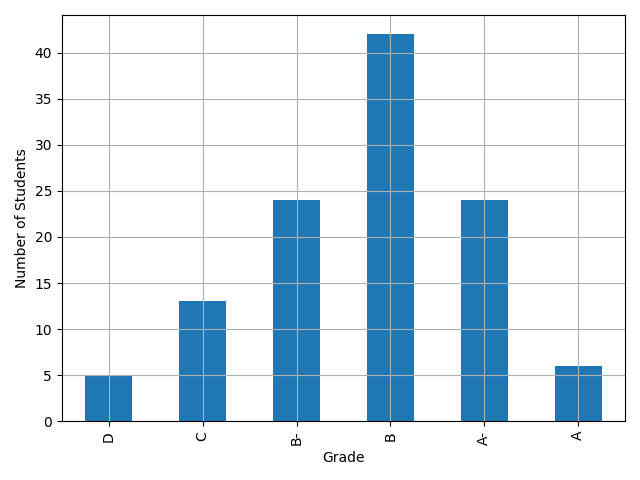
\includegraphics[width=\columnwidth]{grading/figs/grades_gauss.png}
    \caption{Grade distribution using a Gaussian curve.}
    \label{fig:gauss-dist}
\end{figure}
\begin{figure}[!ht]
    \centering
    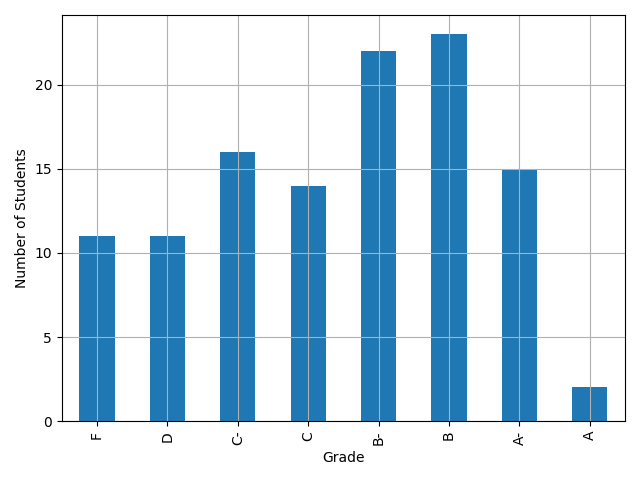
\includegraphics[width=\columnwidth]{grading/figs/grades_kmeans.png}
    \caption{Grade distribution using the $K$-means algorithm.}
    \label{fig:kmeans-dist}
\end{figure}
Based on the results, we can make the following observations:
\begin{enumerate}
    \item Grading using the Gaussian distribution would lead to many students
    failing the course, while this is not the case using the $K$-means
    algorithm.
    \item Using the Gaussian distribution is quite unfair, since there could
    be students with quite similar marks but with a difference in grade, just
    because they lie on either side of a predefined boundary.
    \item The $K$-means algorithm allows for better decision boundaries,
    depending on how skewed the performance of the students is, accordingly
    to the difficulty of the course.
    \item Unlike the Gaussian distribution, the $K$-means algorithm can be
    used for a fairer assignment of the grades, no matter how skewed the 
    performance of students in a course is.
\end{enumerate}

\chapter{Beacon Tracking}
This chpater demonstrates the use of machine learning in beacon tracking using 
an unmanned ground vehicle (UGV) and a WiFi-enabled microcontroller such as the 
ESP32.

\section{Assets}
\begin{enumerate}
    \item UGV chassis with DC motors
    \item ESP32 microcontroller with Type-B USB cable
    \item L293D Motor Driver IC
    \item Breadboard and Jumper Wires
    \item Android phone
    \item (Optional) USB 2.0/3.0 Hub
\end{enumerate}

\section{Procedure}
\begin{enumerate}
    \item Make the connections as per the wiring diagram in Fig. \ref{fig:beacon}.
    \item Connect the ESP32 board to your Android Phone.
    \item Generate the firmware by entering the following commands.
        \begin{lstlisting}
cd ugv-beacon/codes
pio run
        \end{lstlisting}
    \item Go to ArduinoDroid and select
        \begin{lstlisting}[literate={-}{$\rightarrow$ }{1}]
Actions - Upload - Upload Precompiled
        \end{lstlisting}
    and choose the firmware file at
        \begin{lstlisting}
ugv-beacon/codes/.pio/build/firmware.hex
        \end{lstlisting}
    \item Now put the phone at a reasonable distance from the UGV with no 
    obstacles in the way and then turn on the hotspot. The UGV should travel
    towards the phone and stop near it.
\end{enumerate}

\begin{figure}[!ht]
    \centering
    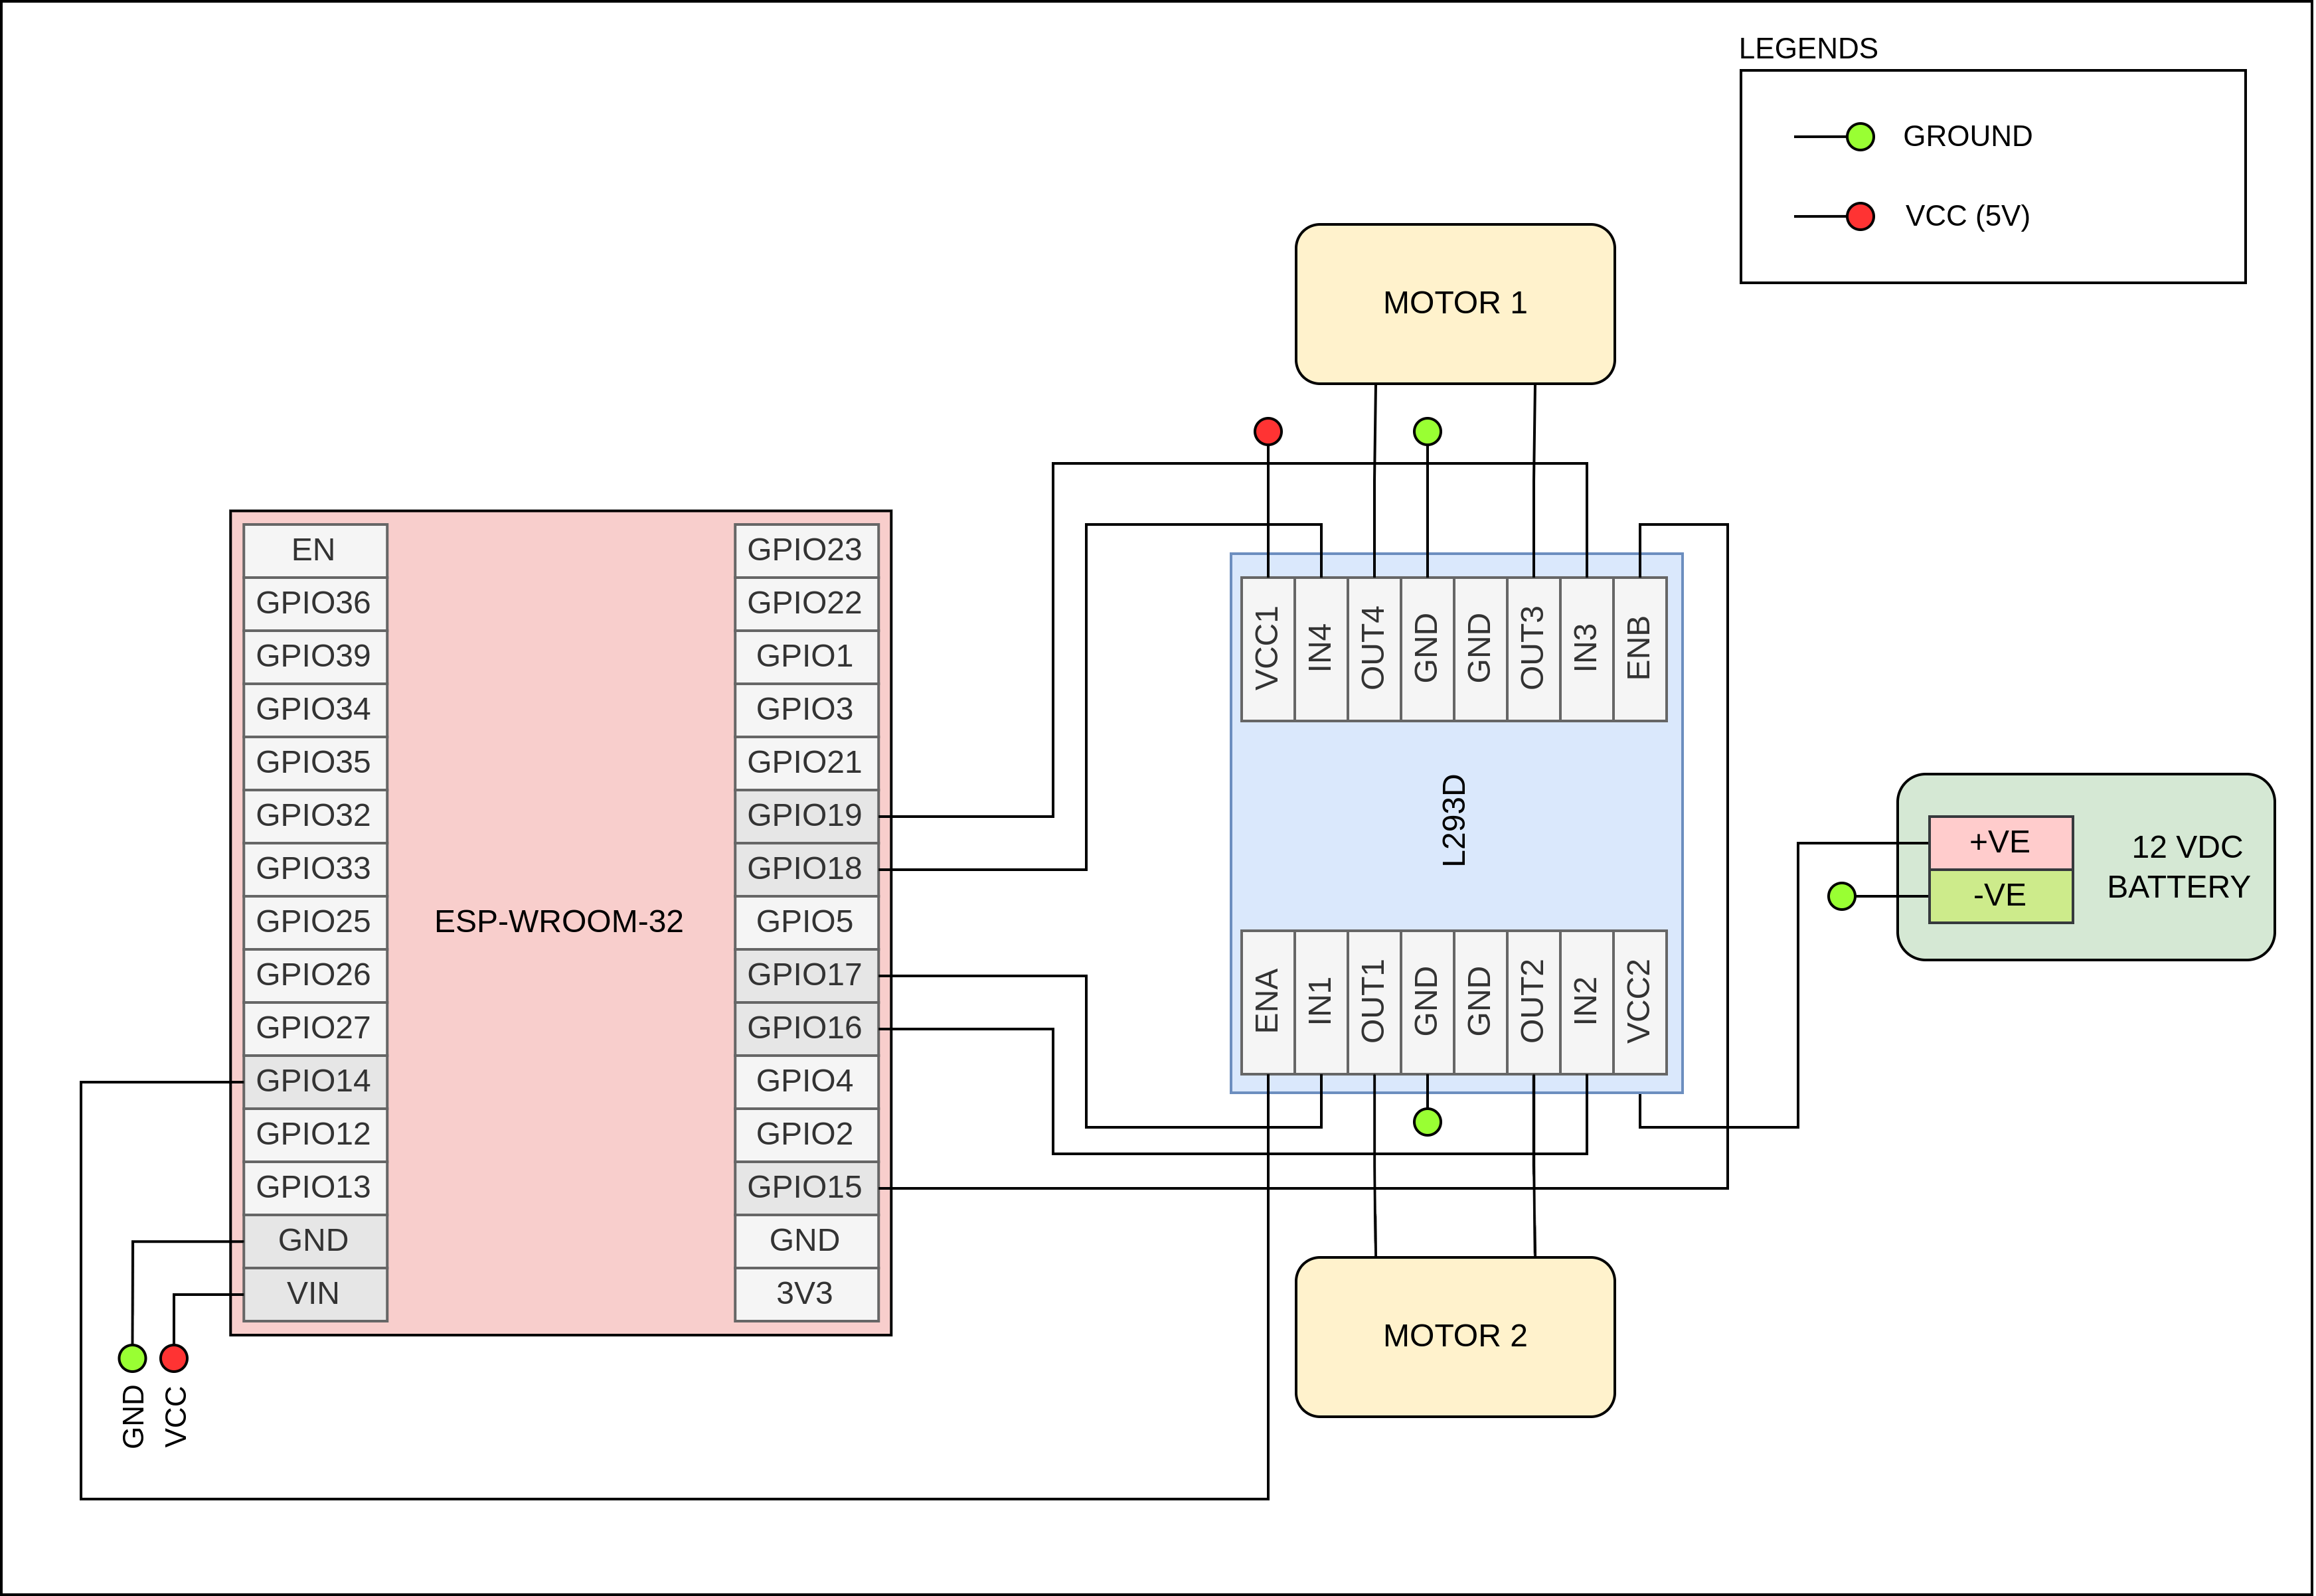
\includegraphics[width=\columnwidth]{ugv-beacon/figs/beacon.png}
    \caption{Wiring Diagram for Beacon Tracking.}
    \label{fig:beacon}
\end{figure}

\section{Working}
\subsection{Underlying Principles}
\begin{enumerate}
    \item To estimate (radial) distance to beacon, we use its signal strength.
        For WiFi, this is the \textbf{Received Signal Strength Indicator} (RSSI).
    \item The RSSI ($R$ dBm) at distance $d$ metres is given by
    \begin{align}
        R(d) = R(1) - 10\log_{10}\brak{d}
    \end{align}
    \item Clearly, $R(d)$ is a convex function. Hence, we can use gradient 
    descent.
\end{enumerate}

\subsection{Algorithm Description}
Please note that this is a generic description of the algorithm employed. Refer to
\begin{lstlisting}
ugv-beacon/codes/src/main.cpp
\end{lstlisting}
for a more verbose implementation.
\begin{enumerate}
    \item If the UGV is close enough to the beacon, \textit{terminate}.
    \item Take measurements at various points on a straight line.
    \item Based on these measurements, decide the next move of the UGV, and 
    recurse till the UGV is close enough to the beacon.
\end{enumerate}

\section{Observations}
\begin{enumerate}
    \item The UGV eventually converges close to the beacon (here, the hotspot).
    \item However, if there are a lot of nearby obstacles, the UGV may not 
    converge close to the location of the beacon. It may either get physically 
    blocked by the beacon or the signal interference may be too high.
\end{enumerate}

\chapter{TinyML}
This chapter illustrates a use case of TinyML in gesture detection. A video
demonstration of the experiment described below is present in the 
\href{https://github.com/gadepall/aiml#TinyML}{README} of the repository.

\section{Assets}
\begin{enumerate}
    \item Android phone
    \item USB 2.0/3.0 hub or USB-OTG
    \item LC Vaman board
\end{enumerate}

\section{Training Data}
\begin{enumerate}
    \item Download the Sensor Logger app from Google Play Store.
    \item In the settings on the app, set the sampling frequency up to 100 Hz, 
    and turn off logging uncalibrated data.
    \item Press \texttt{Start Recording}, and perform the gestures 100 times
    to gather the data.
    \item Press \texttt{Stop Recording} when you are done and export the 
    recordings as a zip file.
    \item Unzip and rename the CSV files appropriately in
    \begin{lstlisting}
tiny-ml/data
    \end{lstlisting}
    \item In the same directory, run the following commands:
    \begin{lstlisting}
gcc -O2 format.c
./a.out
    \end{lstlisting}
    \item Two more CSV files \texttt{train.csv} and \texttt{test.csv} will be 
    created in the same directory.
\end{enumerate}

\section{Model}
\begin{enumerate}
    \item Run the Python script
    \begin{lstlisting}
tiny-ml/codes/bin_class.py
    \end{lstlisting}
    \item Tweak the neural network parameters in this file if the accuracy is
    not satisfactory.
    \item The neural network model will be present as a bytestream in
    \begin{lstlisting}
tiny-ml/codes/client/src/gesture_model.h  
    \end{lstlisting}
\end{enumerate}

\section{Implementation}
\begin{enumerate}
    \item Find the IP address of your phone by using the \texttt{ifconfig}
    command.
    \item In the Sensor Logger app, set the HTTP Push URL to
    \begin{lstlisting}
http://<IP>:5000/gesture
    \end{lstlisting}
    in the app settings. Enable the HTTP Push feature.
    \item In \texttt{tiny-ml/codes/server}, run the following command:
    \begin{lstlisting}
flask run --host <IP>
    \end{lstlisting}
    \item In \texttt{tiny-ml/codes/client}, compile and upload the 
    \textit{platformio} project using USB-UART.
    \item Attach a serial monitor to the terminal with the following command:
    \begin{lstlisting}
pio device monitor -b 115200
    \end{lstlisting}
    \item Start recording in the Sensor Logger app and perform the gestures.
    Verify whether the model works as intended.
    \item Implement a decade counter which can increment and decrement the 
    displayed value based on the detected gesture.
\end{enumerate}

\chapter{Picoprobe}
This chapter enumerates the steps needed to use one Raspberry Pi Pico to debug
another Raspberry Pi Pico from the command line using OpenOCD and GDB. For
further details refer to the
\href{https://www.raspberrypi.com/documentation/microcontrollers/raspberry-pi-pico.html#debugging-using-another-raspberry-pi-pico}{documentation}.

Note that these instructions are for Linux systems running Debian-based
distributions only. For other operating systems refer to the above link.

\section{Assets}
\begin{enumerate}
    \item Two Raspberry Pi Pico boards.
    \item Female-to-female and Male-to-female jumper wires.
    \item One B-type USB cable.
    \item A laptop running a Debian-based Linux distribution such as Ubuntu. 
\end{enumerate}

\section{Setup}
\begin{enumerate}
    \item Setup the Raspberry Pi Pico environment on your laptop by entering the
    following commands at a terminal window.

    \begin{lstlisting}
sudo apt update && sudo apt upgrade
sudo apt install pkg-config
cd
wget https://raw.githubusercontent.com/raspberrypi/pico-setup/master/pico_setup.sh
chmod +x ./pico_setup.sh
SKIP_VSCODE=1 INCLUDE_PICOPROBE=1 ./pico_setup.sh
    \end{lstlisting}

    \item Download the picoprobe file from this 
    \href{https://www.raspberrypi.com/documentation/microcontrollers/raspberry-pi-pico.html#debugging-using-another-raspberry-pi-pico}{link}.
    \item Connect the Raspberry Pi Pico board to be used as the debugger
    (henceforth referred to as the ``debugger'') to your laptop and
    simultaneously press the BOOTSEL button to boot the debugger in bootloader
    mode.
    \item Flash the downloaded \texttt{picoprobe.uf2} file using
    \texttt{picotool} to the debugger as follows.
    \begin{lstlisting}
picotool save /path/to/picoprobe.uf2
    \end{lstlisting}
    \item Wire the debugger to the other Raspberry Pi Pico board by following
    the wiring diagram in \autoref{fig:picoprobe}.
    \begin{figure}[!ht]
        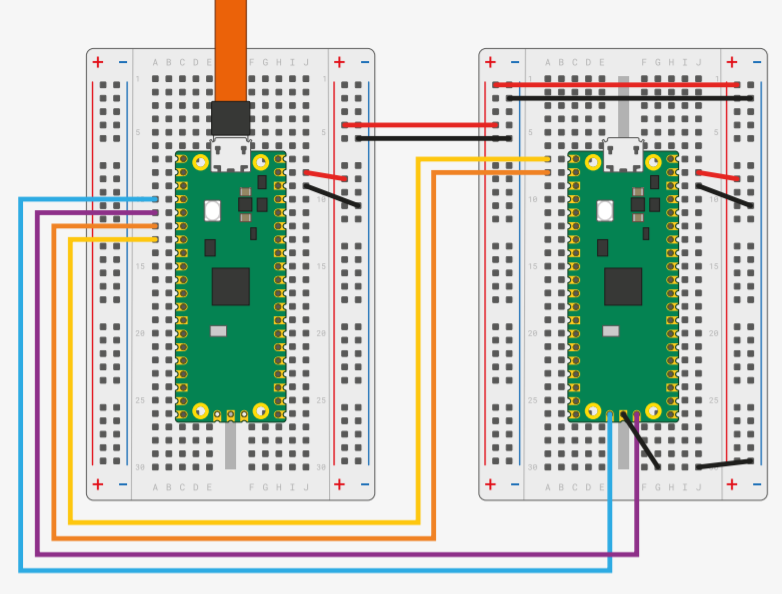
\includegraphics[width=\columnwidth]{picoprobe/figs/picoprobe.png}
        \caption{Wiring diagram to debug a Pico (right) using another Pico as Picoprobe (left).}
        \label{fig:picoprobe}
    \end{figure}
\end{enumerate}

\section{Building}
\begin{enumerate}
    \item Build a debuggable ELF file to load onto the Pico by entering the
    following commands at a terminal window.
    \begin{lstlisting}
cd ~/pico/pico-examples/build
rm -rf ./*
source ~/.bashrc
cmake -DCMAKE_BUILD_TYPE=Debug ..
cd hello_world/serial
make -j4
    \end{lstlisting}
    \item A successful build should generate the debuggable ELF file
    \begin{lstlisting}
~/pico/pico-examples/build/hello_world/serial/hello_serial.elf
    \end{lstlisting}
\end{enumerate}

\section{Debugging}
\begin{enumerate}
    \item Connect the debugger to the laptop again and simultaneously press the
    BOOTSEL button on the target Pico board (and \emph{not} the debugger) to
    boot it in bootloader mode.
    \item In a terminal window, start an OpenOCD server by entering the
    following commands.
    \begin{lstlisting}
cd ~/pico/openocd
sudo src/openocd -f tcl/interface/cmsis-dap.cfg -f tcl/target/rp2040.cfg -s tcl -c "adapter speed 5000"
    \end{lstlisting}
    A successful execution of these commands will result in the following
    (truncated) output.
    \begin{lstlisting}
Info: Listening on port 3333 for gdb connections
    \end{lstlisting}
    \item In \emph{another} terminal window, start \texttt{gdb} with the ELF
    file as follows.
    \begin{lstlisting}
cd ~/pico/pico-examples/build/hello_world/serial
gdb-multiarch hello_serial.elf
(gdb) target remote localhost:3333
(gdb) monitor reset init
(gdb) break main
(gdb) continue
    \end{lstlisting}
    Here, you should see the source code for the program flashed onto the target
    Pico.

    \emph{(Optional)} You can also use \texttt{tmux} instead of two separate
    terminal instances.
    \item You can execute instruction by instruction by typing \texttt{next} at
    the GDB prompt. Alternatively, you can step into functions called from the
    main function by \texttt{step}. 
    \item To reset to the start of the program and reach the main breakpoint
    again, type the following.
    \begin{lstlisting}
(gdb) monitor reset init
(gdb) continue
    \end{lstlisting}
    To quit from gdb, type the following.
    \begin{lstlisting}
(gdb) quit
    \end{lstlisting}
    For other functionalities type \texttt{help} at the GDB
    prompt.
    \item To see serial output, attach a terminal to the device by typing the
    following commands at a terminal window.
    \begin{lstlisting}
sudo minicom -D /dev/ttyACM0 -b 115200
    \end{lstlisting}
    Note that if the device is not present at \texttt{/dev/ttyACM0}, then you
    can find the correct port by inspecting the output produced by the
    following command.
    \begin{lstlisting}
sudo dmesg -w
    \end{lstlisting}
\end{enumerate}
\iffalse
\chapter{Convex Functons}
\section{Definition}
\renewcommand{\theequation}{\theenumi}
%\subsection{Problem}

\begin{enumerate}[label=\thesection.\arabic*.,ref=\thesection.\theenumi]
\numberwithin{equation}{enumi}

\item
The following python script plots 
%
\begin{align}
f(\lambda) = a\lambda^2 + b\lambda + d
\label{eq:opt_parab}
\end{align}
%
for 
\begin{align}
a &= \norm{\vec{m}}^2 > 0
\\
b &= \vec{m}^T\brak{\vec{A} -\vec{P}} 
\\
c &= \norm{\vec{A} -\vec{P}}^2
\end{align}
where $\vec{A}$ is the intercept of the line $L$ in \eqref{eq:opt_line_nor}
on the x-axis and the points
\begin{align}
\vec{U} &= \myvec{\lambda_1\\f(\lambda_1)}, 
\vec{V} = \myvec{\lambda_2\\f(\lambda_2)}
\\
\vec{X} &= \myvec{t \lambda_1 + \brak{1-t}\lambda_2 \\ f\sbrak{t \lambda_1 + \brak{1-t}\lambda_2}},
\\
\vec{Y} &= \myvec{t \lambda_1 + \brak{1-t}\lambda_2 \\ t f\brak{\lambda_1} + \brak{1-t}f\brak{\lambda_2}}
\end{align}
%
for 
\begin{align}
\lambda_1 = -3, 
\lambda_2 = 4, 
t = 0.3
\end{align}
in Fig. \ref{fig:conv_def}. Geometrically, this means that any point $\vec{Y}$ between the points $\vec{U}, \vec{V}$ on the line $UV$ is always above the point $\vec{X}$ on the curve $f(\lambda)$.
Such a  function $f$ is defined to be {\em convex} function 
%
\begin{lstlisting}
opt/codes/1.2.py
\end{lstlisting}
%
%%
\begin{figure}[!ht]
\centering
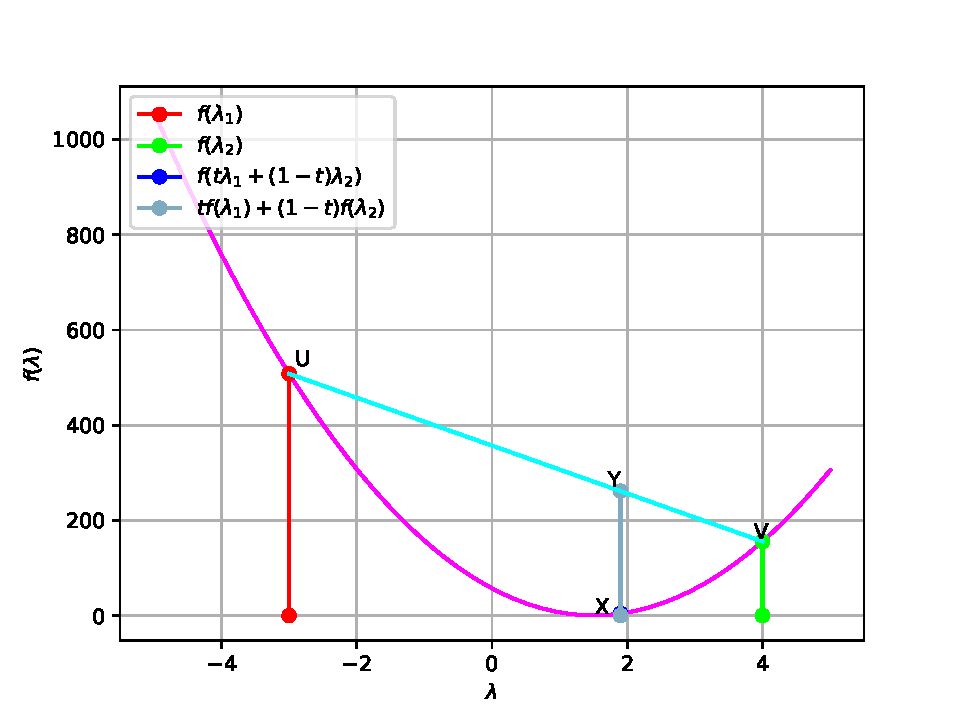
\includegraphics[width=\columnwidth]{./opt/figs/convex.eps}
\caption{ $f(\lambda)$ versus $\lambda$}.
\label{fig:conv_def}	
\end{figure}
%
\item Show that
%
\begin{align}
\label{eq:convex_def}
f\sbrak{t \lambda_1 + \brak{1-t}\lambda_2} \leq 
t f\brak{\lambda_1} + \brak{1-t}f\brak{\lambda_2}
\end{align}
%
for $\quad 0 < t < 1$.  This is true for any convex function.
%
\item Show that 
%
\begin{equation}
\eqref{eq:convex_def} \quad \implies f^{(2)}(\lambda) > 0
\end{equation}
%
\item Show that a covex function has a unique minimum.
%
\end{enumerate}
%


\section{Convex Examples}
\begin{enumerate}[label=\thechapter.\arabic*,ref=\thechapter.\theenumi]
\numberwithin{equation}{enumi}
\numberwithin{figure}{enumi}
\numberwithin{table}{enumi}
\item Reduce $x-\sqrt{3}y+8=0$ into normal form. Find its perpendicular distance from the origin and angle between perpendicular and the positive x-axis. 
			\\
\solution 
\label{11/10/3/3/1/conv}
\iffalse
\documentclass[12pt]{article}
\usepackage{graphicx}
\usepackage[none]{hyphenat}
\usepackage{graphicx}
\usepackage{listings}
\usepackage[english]{babel}
\usepackage{graphicx}
\usepackage{caption} 
\usepackage{booktabs}
\usepackage{array}
\usepackage{amssymb} % for \because
\usepackage{amsmath}   % for having text in math mode
\usepackage{extarrows} % for Row operations arrows
\usepackage{listings}
\lstset{
  frame=single,
  breaklines=true
}
\usepackage{hyperref}
  
%Following 2 lines were added to remove the blank page at the beginning
\usepackage{atbegshi}% http://ctan.org/pkg/atbegshi
\AtBeginDocument{\AtBeginShipoutNext{\AtBeginShipoutDiscard}}
\usepackage{gensymb}


%New macro definitions
\newcommand{\mydet}[1]{\ensuremath{\begin{vmatrix}#1\end{vmatrix}}}
\providecommand{\brak}[1]{\ensuremath{\left(#1\right)}}
\providecommand{\sbrak}[1]{\ensuremath{{}\left[#1\right]}}
\providecommand{\norm}[1]{\left\lVert#1\right\rVert}
\providecommand{\abs}[1]{\left\vert#1\right\vert}
\newcommand{\solution}{\noindent \textbf{Solution: }}
\newcommand{\myvec}[1]{\ensuremath{\begin{pmatrix}#1\end{pmatrix}}}
\let\vec\mathbf


\begin{document}

\begin{center}
\title{\textbf{Convex Optimization}}
\date{\vspace{-5ex}} %Not to print date automatically
\maketitle
\end{center}
\setcounter{page}{1}

\section{11$^{th}$ Maths - Chapter 10}
This is Problem-3.1 from Exercise 10.3 
\begin{enumerate}

\solution 
\fi
Let $\vec{O}$ be the point from where we have to find the perpendicular distance and $\vec{P}$ be the foot of the perpendicular. The optimization problem can be expressed as
\begin{align}
	\label{eq:11/10/3/3/1/conv/Eq3}
	  \min_{\vec{x}} \norm{\vec{x}-\vec{O}}^2\\
	 \text{s.t.} \quad \vec{n}^T\vec{x} = c 
\end{align}
where 
\begin{align}
	\vec{n} = \myvec{-1 \\ \sqrt{3}},\,c = 8
\end{align}
The line equation can be expressed as
\begin{align}
	\label{eq:11/10/3/3/1/conv/Eq2}
	\vec{x} = \vec{A}+\lambda\vec{m}
\end{align}
where
\begin{align}
	\label{eq:11/10/3/3/1/conv/Eq1}
	\vec{m} = \myvec{1 \\ \frac{1}{\sqrt{3}}},\,
	\vec{A} = \myvec{-8 \\ 0}
\end{align}
\begin{enumerate}
\item Using the parameric form,
Substituting \eqref{eq:11/10/3/3/1/conv/Eq2} in \eqref{eq:11/10/3/3/1/conv/Eq3}, the optimization problem becomes
\begin{align}
	\min_{\lambda} \norm{ \lambda\vec{m} +\brak{\vec{A}-\vec{O}}}^2\\
	\implies \min_{\lambda}f\brak{\lambda} 	
	= \lambda^2\norm{\vec{m}}^2+ 2\lambda\brak{\vec{A}-\vec{O}}^\top\vec{m}+ + \norm{\vec{A}-\vec{O}}^2  
\label{eq:11/10/3/3/1/conv/Eq4}
\end{align}
$\because$ the coefficient of $\lambda^2> 0$, \eqref{eq:11/10/3/3/1/conv/Eq4} is a convex function.
Thus,
\begin{align}
	f^{\prime\prime}\brak{\lambda} &= 2\norm{\vec{m}}^2 \\ 
	\because f^{\prime\prime}\brak{\lambda} > 0, f^\prime\brak{\lambda_{min}} &= 0, \text{ for } \lambda_{min}
\end{align}
yielding
\begin{align}
	& f^\prime\brak{\lambda_{min}} =  2\lambda_{min}\norm{\vec{m}}^2 + 2\brak{\vec{A}-\vec{O}}^\top\vec{m}  = 0 \\
	\label{eq:11/10/3/3/1/conv/EqMin}
	\lambda_{min} &= -\frac{\brak{\vec{A}-\vec{O}}^\top\vec{m}}{\norm{\vec{m}}^2} 
\end{align}
We choose  
\begin{align}
	\vec{O} &= \myvec{ 0 \\ 0}
\end{align}
Substituting the values of $\vec{A}$, $\vec{O}$ and $\vec{m}$ in equation \eqref{eq:11/10/3/3/1/conv/EqMin}
\begin{align}
	\lambda_{min} &= -\frac{\brak{\myvec{-8 \\ 0 }-\myvec{0 \\ 0}}^\top\myvec{1 \\ \frac{1}{\sqrt{3}}}}{\norm{\myvec{1 \\ \frac{1}{\sqrt{3}}}}^2}\\ 
	&= 6
\end{align}
Substituring this value in equation \eqref{eq:11/10/3/3/1/conv/Eq2}
\begin{align}
	\vec{x}_{min} &= \vec{P} = \myvec{-8 \\ 0}+6\myvec{1 \\ \frac{1}{\sqrt{3}}}  \\
	&= \myvec{-2 \\ 2\sqrt{3}} \\
	OP &= \norm{\vec{P}-\vec{O}}^2 \\ 
	&  = 4
\end{align}
\item Solving using cvxpy, with 
\begin{align}
	&\vec{n} = \myvec{1 \\ -\sqrt{3}} \\
	&\vec{O} = \myvec{0 \\ 0} \\
	&c = -8 \\
	\label{eq:11/10/3/3/1/conv/minval}
	&  \min_{\vec{x}} \norm{\vec{x}-\vec{O}}^2 = 4, 
	 \vec{x}_{min} = \myvec{-2  \\ 3.46 } 
\end{align}
\end{enumerate}
The relevant figures are shown in \ref{fig:11/10/3/3/1/conv/Fig1} and \ref{fig:11/10/3/3/1/conv/Fig2}
\begin{figure}[!h]
	\begin{center}
		\includegraphics[width=\columnwidth]{11/10/3/3/1/conv/figs/problem3.1a.pdf}
	\end{center}
\caption{}
\label{fig:11/10/3/3/1/conv/Fig1}
\end{figure}
\begin{figure}[!h]
	\begin{center}
		\includegraphics[width=\columnwidth]{11/10/3/3/1/conv/figs/problem3.1b.pdf}
	\end{center}
\caption{}
\label{fig:11/10/3/3/1/conv/Fig2}
\end{figure}

		\item Reduce the equation $y-2=0$ into normal form. Find the perpendicular distances from the origin and angle between perpendicular and the positive x-axis.
			\\
\solution 
\label{11/10/3/3/2/conv}
\iffalse
\documentclass[12pt]{article}
\usepackage{graphicx}
\usepackage{amsmath}
\usepackage{mathtools}
\usepackage{gensymb}
\usepackage{tabularx}
\usepackage{array}
\usepackage[latin1]{inputenc}
\usepackage{fullpage}
\usepackage{color}
\usepackage{array}
\usepackage{longtable}
\usepackage{calc}
\usepackage{multirow}
\usepackage{hhline}
\usepackage{ifthen}
\usepackage{lscape}
\usepackage{float}
\usepackage{amssymb}

\newcommand{\mydet}[1]{\ensuremath{\begin{vmatrix}#1\end{vmatrix}}}
\providecommand{\brak}[1]{\ensuremath{\left(#1\right)}}
\providecommand{\norm}[1]{\left\lVert#1\right\rVert}
\providecommand{\abs}[1]{\left\vert#1\right\vert}
\newcommand{\solution}{\noindent \textbf{Solution: }}
\newcommand{\myvec}[1]{\ensuremath{\begin{pmatrix}#1\end{pmatrix}}}
\let\vec\mathbf

\def\inputGnumericTable{}

\begin{document}
\begin{center}
\textbf\large{OPTIMIZATION}

\end{center}
\section*{Excercise 10.3}


\solution
\fi
The given equation can be written as
\begin{align}
	\label{eq:11/10/3/3/2/conv/eq1}
	\myvec{0&1}\vec{x} &= 2\\
\implies 	\vec{n} &= \myvec{0\\1},\,
	\vec{m} = \myvec{1\\0}
\end{align}
Equation \eqref{eq:11/10/3/3/2/conv/eq1} can be represented in parametric form as
\begin{align}
	\label{eq:11/10/3/3/2/conv/eq2}
	\vec{x} = \vec{A}+\lambda\vec{m}
\end{align}
where
\begin{align}
	\vec{A} &= \myvec{2\\2}.
	\label{eq:11/10/3/3/2/conv/line}
\end{align}
Let $\vec{O}$ be the origin. The perpendicular distance will be the minimum distance from $\vec{O}$ to the line. Let $\vec{P}$ be the foot of perpendicular. This problem can be formulated as an optimization problem as 
\begin{align}
	d &=  \min_{\vec{x}}\norm{\vec{x}-\vec{O}}^2\\
	&=\min_{\lambda}\norm{\vec{A}+\lambda\vec{m}-\vec{O}}^2\\
	&= f\brak{\lambda} = \norm{\vec{m}}^2\lambda^2+2\vec{A}^\top\vec{m}+\norm{\vec{A}}^2
	\label{eq:11/10/3/3/2/conv/eq3}
	\\
	&= \lambda^2+4\lambda+8
\end{align}
$\because$ the coefficient of $\lambda^2>0$, \eqref{eq:11/10/3/3/2/conv/eq3} is convex. 
\begin{align}
	\label{eq:11/10/3/3/2/conv/eq4}
	f^\prime\brak{\lambda} = 2\norm{\vec{m}}^2\lambda+\brak{\vec{A}^\top\vec{m}+\vec{m}^\top\vec{A}}
\end{align}
\begin{enumerate}
\item Computing $\lambda_{min}$ using Derivative method
\begin{align}
	f^{\prime\prime}\brak{\lambda} &= 2\\
	\because f^{\prime\prime}\brak{\lambda}>0,&f^{\prime}\brak{\lambda_{min}}=0, \text{ for } \lambda_{min}\\
	f^{\prime}\brak{\lambda_{min}} &= 2\norm{\vec{m}}^2\lambda_{min}+\brak{\vec{A}^\top\vec{m}+\vec{m}^\top\vec{A}}\\
	\therefore \lambda_{min} &= -\frac{\brak{\vec{A}^\top\vec{m}+\vec{m}^\top\vec{A}}}{2\norm{\vec{m}}^2} = -2
\end{align}
Thus, 
\begin{align}
	\vec{x}_{min} &= \vec{P} = \myvec{2\\2}+\brak{-2}\myvec{1\\0}\\
	&= \myvec{0\\2}\\
	OP &= \norm{\vec{P}-\vec{O}}\\
	&= \norm{\myvec{0\\2}-\myvec{0\\0}}\\
	&= 2
\end{align}
\item Solving using cvxpy, with
\begin{align}
	\vec{n} &= \myvec{0\\1}\\
	\vec{O} &= \myvec{0\\0}\\
	c &= 2\\
	&\min_{\vec{x}}\norm{\vec{x}-\vec{O}}^2 = 2, \vec{x}_{min} = \myvec{0\\2}
\end{align}
\end{enumerate}
See Figs. \ref{fig:11/10/3/3/2/conv/Fig1} and \ref{fig:11/10/3/3/2/conv/Fig2}.
\begin{figure}[!h]
	\begin{center} 
	    \includegraphics[width=\columnwidth]{11/10/3/3/2/conv/figs/opt1}
	\end{center}
\caption{}
\label{fig:11/10/3/3/2/conv/Fig1}
\end{figure}
\begin{figure}[!h]
	\begin{center} 
	    \includegraphics[width=\columnwidth]{11/10/3/3/2/conv/figs/opt2}
	\end{center}
\caption{}
\label{fig:11/10/3/3/2/conv/Fig2}
\end{figure}

 \item Find the coordinates of the foot of perpendicular from the point 
    \begin{align}
        \vec{P} = \myvec{-1\\3}
        \label{eq:11/10/3/14/conv/P-def}
    \end{align}
    to the line 
    \begin{align}
        \myvec{3&-4}\vec{x} = 16
        \label{eq:11/10/3/14/conv/line}
    \end{align}
			\\
\solution 
\label{11/10/3/14/conv}
\iffalse
\documentclass[journal,12pt,twocolumn]{IEEEtran}
\usepackage{setspace}
\usepackage{gensymb}
\singlespacing
\usepackage[cmex10]{amsmath}
\usepackage{amsthm}
\usepackage{mathrsfs}
\usepackage{txfonts}
\usepackage{stfloats}
\usepackage{bm}
\usepackage{cite}
\usepackage{cases}
\usepackage{subfig}
\usepackage{longtable}
\usepackage{multirow}
\usepackage{enumitem}
\usepackage{mathtools}
\usepackage{tikz}
\usepackage{circuitikz}
\usepackage{verbatim}
\usepackage[breaklinks=true]{hyperref}
\usepackage{tkz-euclide} % loads  TikZ and tkz-base
\usepackage{listings}
\usepackage{color}    
\usepackage{array}    
\usepackage{longtable}
\usepackage{calc}     
\usepackage{multirow} 
\usepackage{hhline}   
\usepackage{ifthen}   
\usepackage{lscape}     
\usepackage{chngcntr}
\DeclareMathOperator*{\Res}{Res}
\renewcommand\thesection{\arabic{section}}
\renewcommand\thesubsection{\thesection.\arabic{subsection}}
\renewcommand\thesubsubsection{\thesubsection.\arabic{subsubsection}}

\renewcommand\thesectiondis{\arabic{section}}
\renewcommand\thesubsectiondis{\thesectiondis.\arabic{subsection}}
\renewcommand\thesubsubsectiondis{\thesubsectiondis.\arabic{subsubsection}}
\renewcommand\thetable{\arabic{table}}
% correct bad hyphenation here
\hyphenation{op-tical net-works semi-conduc-tor}
\def\inputGnumericTable{}                                 %%

\lstset{
%language=C,
frame=single, 
breaklines=true,
columns=fullflexible
}
%\lstset{
%language=tex,
%frame=single, 
%breaklines=true
%}

\begin{document}
\newtheorem{theorem}{Theorem}[section]
\newtheorem{problem}{Problem}
\newtheorem{proposition}{Proposition}[section]
\newtheorem{lemma}{Lemma}[section]
\newtheorem{corollary}[theorem]{Corollary}
\newtheorem{example}{Example}[section]
\newtheorem{definition}[problem]{Definition}
\newcommand{\BEQA}{\begin{eqnarray}}
\newcommand{\EEQA}{\end{eqnarray}}
\newcommand{\define}{\stackrel{\triangle}{=}}
\bibliographystyle{IEEEtran}
\providecommand{\mbf}{\mathbf}
\providecommand{\pr}[1]{\ensuremath{\Pr\left(#1\right)}}
\providecommand{\qfunc}[1]{\ensuremath{Q\left(#1\right)}}
\providecommand{\sbrak}[1]{\ensuremath{{}\left[#1\right]}}
\providecommand{\lsbrak}[1]{\ensuremath{{}\left[#1\right.}}
\providecommand{\rsbrak}[1]{\ensuremath{{}\left.#1\right]}}
\providecommand{\brak}[1]{\ensuremath{\left(#1\right)}}
\providecommand{\lbrak}[1]{\ensuremath{\left(#1\right.}}
\providecommand{\rbrak}[1]{\ensuremath{\left.#1\right)}}
\providecommand{\cbrak}[1]{\ensuremath{\left\{#1\right\}}}
\providecommand{\lcbrak}[1]{\ensuremath{\left\{#1\right.}}
\providecommand{\rcbrak}[1]{\ensuremath{\left.#1\right\}}}
\theoremstyle{remark}
\newtheorem{rem}{Remark}
\newcommand{\sgn}{\mathop{\mathrm{sgn}}}
\providecommand{\abs}[1]{\left\vert#1\right\vert}
\providecommand{\res}[1]{\Res\displaylimits_{#1}} 
\providecommand{\norm}[1]{\left\lVert#1\right\rVert}
\providecommand{\mtx}[1]{\mathbf{#1}}
\providecommand{\mean}[1]{E\left[ #1 \right]}
\providecommand{\fourier}{\overset{\mathcal{F}}{ \rightleftharpoons}}
\providecommand{\system}[1]{\overset{\mathcal{#1}}{ \longleftrightarrow}}
\newcommand{\solution}{\noindent \textbf{Solution: }}
\newcommand{\cosec}{\,\text{cosec}\,}
\providecommand{\dec}[2]{\ensuremath{\overset{#1}{\underset{#2}{\gtrless}}}}
\newcommand{\myvec}[1]{\ensuremath{\begin{pmatrix}#1\end{pmatrix}}}
\newcommand{\mydet}[1]{\ensuremath{\begin{vmatrix}#1\end{vmatrix}}}
\let\vec\mathbf
\def\putbox#1#2#3{\makebox[0in][l]{\makebox[#1][l]{}\raisebox{\baselineskip}[0in][0in]{\raisebox{#2}[0in][0in]{#3}}}}
     \def\rightbox#1{\makebox[0in][r]{#1}}
     \def\centbox#1{\makebox[0in]{#1}}
     \def\topbox#1{\raisebox{-\baselineskip}[0in][0in]{#1}}
     \def\midbox#1{\raisebox{-0.5\baselineskip}[0in][0in]{#1}}

\vspace{3cm}
\title{Optimization Assignment}
\author{Gautam Singh}
\maketitle
\bigskip

\begin{abstract}
    This document contains the solution to Question 4 of Exercise 2 in Chapter
    10 of the class 11 NCERT textbook.
\end{abstract}

\begin{enumerate}
   
    \solution 
    \fi
		Any point on \eqref{eq:11/10/3/14/conv/line} is clearly of the form
    \begin{align}
        \vec{Q} = \vec{A} + \lambda\vec{m}
        \label{eq:11/10/3/14/conv/Q-def}
    \end{align}
    where $\lambda \in \mathbb{R}$ and
    \begin{align}
        \vec{A} = \myvec{0\\-4},\ \vec{m} = \myvec{4\\3}
        \label{eq:11/10/3/14/conv/vals}
    \end{align}
    Thus,
    \begin{align}
        f\brak{\lambda} &= \norm{\vec{Q}-\vec{P}}^2 \\
                        &= \norm{\vec{A}-\vec{P}+\lambda\vec{m}}^2 \\
                        &= \norm{\vec{m}}^2\lambda^2 + 2\vec{m}^\top\brak{\vec{A}-\vec{P}}\lambda + \norm{\vec{A}-\vec{P}}^2
                        \label{eq:11/10/3/14/conv/dist-lambda}
    \end{align}
    Since the coefficient of $\lambda^2$ in $f(\lambda)$ is positive, it
    follows that $f\brak{\lambda}$ is convex. Hence, the minima is achieved at
    \begin{align}
        f'\brak{\lambda_m} &= 2\brak{\norm{\vec{m}}^2\lambda_m + \vec{m}^\top\brak{\vec{A}-\vec{P}}} = 0 \\
        \implies \lambda_m &= -\frac{\vec{m}^\top\brak{\vec{A}-\vec{P}}}{\norm{\vec{m}}^2}
        \label{eq:11/10/3/14/conv/lambda-min}
    \end{align}
    Thus,
    \begin{align}
        \vec{Q_m} &= \vec{A} + \lambda_m\vec{m} \\
                  &= \vec{A} - \frac{\vec{m}^\top\brak{\vec{A}-\vec{P}}}{\norm{\vec{m}}^2}\vec{m}
                  \label{eq:11/10/3/14/conv/Q-m-exp}
    \end{align}
    Thus, substituting \eqref{eq:11/10/3/14/conv/vals} into \eqref{eq:11/10/3/14/conv/Q-m-exp}, we get
    \begin{align}
        \vec{Q_m} = \frac{1}{25}\myvec{68\\-49}
        \label{eq:11/10/3/14/conv/Q-sol}
    \end{align}
    The value of $\lambda_m$ is verified in Fig. \ref{fig:11/10/3/14/conv/convex}.
		\begin{figure}[!ht]
        \centering
        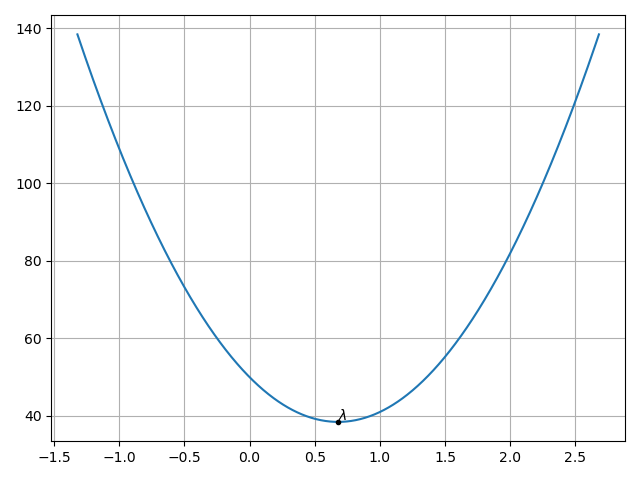
\includegraphics[width=\columnwidth]{11/10/3/14/conv/figs/convex.png}
        \caption{This convex function achieves its minimum at $\lambda_m$.}
        \label{fig:11/10/3/14/conv/convex}
    \end{figure}



	\item Determine if the following are convex functions
\begin{enumerate}
\item Determine whether the function $f\brak{x} = \brak{2x-1}^2 + 3$ is convex or not. \\ 
\solution 
\label{12/6/5/1/1/conv}
%Determine if the following are convex functions
\begin{enumerate}[label=\thechapter.\arabic*,ref=\thechapter.\theenumi]
\numberwithin{equation}{enumi}
\numberwithin{figure}{enumi}
\numberwithin{table}{enumi}
\item
	\begin{enumerate}
\item Detrmine whether the function $f\brak{x} = \brak{2x-1}^2 + 3$ is convex or not. \\ 
\solution 
\label{12/6/5/1/1/conv}
\iffalse 
\documentclass[12pt]{article}
\usepackage{graphicx}
\usepackage[none]{hyphenat}
\usepackage{graphicx}
\usepackage{listings}
\usepackage[english]{babel}
\usepackage{graphicx}
\usepackage{caption} 
\usepackage{booktabs}
\usepackage{array}
\usepackage{amssymb} % for \because
\usepackage{amsmath}   % for having text in math mode
\usepackage{extarrows} % for Row operations arrows
\usepackage{listings}
\lstset{
  frame=single,
  breaklines=true
}
\usepackage{hyperref}
\usepackage{mathtools}

%Following 2 lines were added to remove the blank page at the beginning
\usepackage{atbegshi}% http://ctan.org/pkg/atbegshi
\AtBeginDocument{\AtBeginShipoutNext{\AtBeginShipoutDiscard}}


%New macro definitions
\newcommand{\mydet}[1]{\ensuremath{\begin{vmatrix}#1\end{vmatrix}}}
\providecommand{\brak}[1]{\ensuremath{\left(#1\right)}}
\providecommand{\sbrak}[1]{\ensuremath{{}\left[#1\right]}}
\providecommand{\norm}[1]{\left\lVert#1\right\rVert}
\providecommand{\abs}[1]{\left\vert#1\right\vert}
\newcommand{\solution}{\noindent \textbf{Solution: }}
\newcommand{\myvec}[1]{\ensuremath{\begin{pmatrix}#1\end{pmatrix}}}
\let\vec\mathbf


\begin{document}

\begin{center}
\title{\textbf{Convex Optimization}}
\date{\vspace{-5ex}} %Not to print date automatically
\maketitle
\end{center}
\setcounter{page}{1}

\section{12$^{th}$ Maths - Chapter 6}
This is Problem-1(i) from Exercise 6.5
\begin{enumerate}
		\fi
The given function is 
\begin{align}
        \label{eq:/12/6/5/1/1/convEq5}
	f\brak{x} &= \brak{2x-1}^2 + 3 \\ 
	&= 4x^2+4x+4 \\
	\therefore a &= 4, > 0
\end{align}
Hence, the function in equation \eqref{eq:/12/6/5/1/1/convEq5} is convex
	from \ref{prop:app/convconvconvex_def}.
%
The figure is as shown in Fig\ref{fig:/12/6/5/1/1/convFig1}
\begin{figure}[!h]
	\begin{center}
		\includegraphics[width=\columnwidth]{12/6/5/1/1/1/figs/opt2.pdf}
	\end{center}
\caption{}
\label{fig:/12/6/5/1/1/convFig1}
\end{figure}

	\end{enumerate}
\item
At what points in the interval (0,2$\pi$) does the function $\sin2x$ attain its maximum value.
\label{12/6/5/8/1}
%\iffalse
\documentclass[journal,10pt,twocolumn]{article}
\usepackage{graphicx, float}
\usepackage[margin=0.5in]{geometry}
\usepackage{amsmath, bm}
\usepackage{array}
\usepackage{booktabs}
\usepackage{mathtools}

\providecommand{\norm}[1]{\left\lVert#1\right\rVert}
\let\vec\mathbf
\newcommand{\myvec}[1]{\ensuremath{\begin{pmatrix}#1\end{pmatrix}}}
\newcommand{\mydet}[1]{\ensuremath{\begin{vmatrix}#1\end{vmatrix}}}

\title{\textbf{Optimization Assignment}}
\author{Maddu Dinesh}
\date{September 2022}

\begin{document}

\maketitle
\paragraph{\textit{Problem Statement} -
\fi
At what points in the interval (0,2$\pi$) does the function $\sin2x$ attain its maximum value.
\\
\solution
	\begin{figure}[!ht]
		\centering
		\includegraphics[width=\columnwidth]{12/6/5/8/figs/a.png}
		\caption{}
		\label{fig:12/6/5/8}
  	\end{figure}
\iffalse
\section*{\large Figure}

\begin{figure}[H]
\centering
\includegraphics[width=1\columnwidth]{a.png}
\caption{Graph of f(x)}
\label{fig:triangle}
\end{figure}
\section*{\large Solution}

	
    \subsection*{\normalsize Gradient descent}
\fi    
  Since  
    \begin{align}
	\label{eq:12/6/5/8vol_varx}
	    f(x) &= \sin2x,
	    \\
	    f'(x) &= 2\cos2x
	\end{align}
\iffalse
we have to attain the maximum value of sin2x in the interval [0,2$\pi$]. This can be seen in Figure f(x).
\fi
Using gradient ascent, 
\begin{align}
	x_{n+1} &= x_n + \alpha \nabla f(x_n) \\
&=x_n+\alpha(2\cos2x)
\end{align}
Choosing
\begin{align}
	x_0&=0.5,\alpha=0.001, precision = 0.00000001, 
	\\
	f_{max} &= 1.0000,
 	x_{max}= 0.7854.
    \end{align}
   
    

    





 







\item
Find the absolute maximum and minimum values of the function $f$ given by 
\begin{align}
	f(x) = \cos^2x + \sin x,\quad x \in \sbrak{0,\pi} 
\end{align} 
\label{12/6/6/14/1}
%\iffalse
\documentclass[10pt,twocolumn]{article}
\usepackage{graphicx}
\usepackage[margin=0.5in]{geometry}
\usepackage[cmex10]{amsmath}
\usepackage{array}
\usepackage{booktabs}
\usepackage{mathtools}
\title{\textbf{Optimization Assignment}}
\author{Sinkona Chinthamalla}

\providecommand{\norm}[1]{\lVert#1\rVert}
\providecommand{\abs}[1]{\vert#1\vert}
\let\vec\mathbf
\newcommand{\myvec}[1]{\ensuremath{\begin{pmatrix}#1\end{pmatrix}}}
\newcommand{\mydet}[1]{\ensuremath{\begin{vmatrix}#1\end{vmatrix}}}
\providecommand{\brak}[1]{\ensuremath{\left(#1\right)}}
\providecommand{\lbrak}[1]{\ensuremath{\left(#1\right.}}
\providecommand{\rbrak}[1]{\ensuremath{\left.#1\right)}}
\providecommand{\sbrak}[1]{\ensuremath{{}\left[#1\right]}}

\begin{document}

\maketitle
\paragraph{\textit{Problem Statement} -
\fi
Find the absolute maximum and minimum values of the function $f$ given by 
\begin{align}
	f(x) = \cos^2x + \sin x,\quad x \in \sbrak{0,\pi} 
\end{align} 
\solution
	\begin{figure}[!ht]
		\centering
		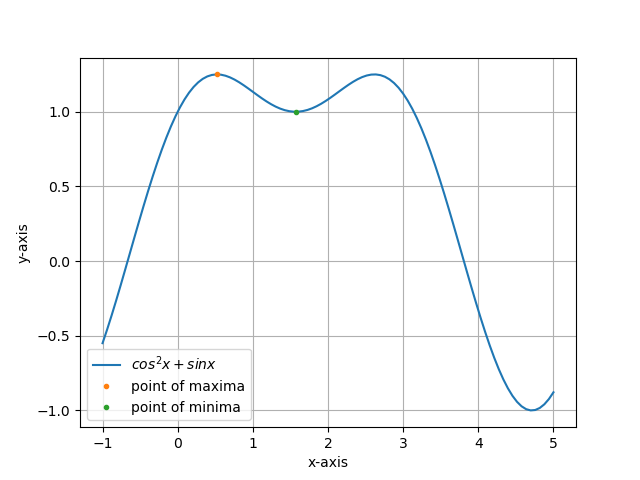
\includegraphics[width=\columnwidth]{12/6/6/14/figs/opt.png}
		\caption{}
		\label{fig:12/6/6/14}
  	\end{figure}
\iffalse

\section{Solution}
\begin{flushleft}
Given function is,\\
\end{flushleft}
\begin{equation}
    f(x)=\cos^2x + \sin x
\end{equation}
\subsection{Calculation using normal differentiation}
\begin{flushleft}
Differentiating (1) yields,
\end{flushleft}
\fi
The derivative of the given function is
\begin{align}
\nabla f(x) = \cos x-2\sin x \cos x 
\end{align}
\iffalse

\noindent Calculating the critical points:
$ \nabla f(x) = 0 $

\begin{equation}
\implies \cos{x} = 0 
\end{equation}
\begin{equation}
\implies -2\sin{x} + 1 = 0
\end{equation}
Therefore, the critical points are 

\begin{equation}
\frac{\pi}{6},\quad\frac{5\pi}{6},\quad\frac{\pi}{2}
\end{equation}

\textbf{1.1.1 Finding absolute maximum and minimum} 
Since given interval is $x \in [0,\pi]$ 

\begin{table}[h]
\centering
\large
\begin{tabular}{|l|l|}
\hline
\textbf{value of x} & \textbf{value of} \\ \hline
At x =0             & 1                 \\ \hline
At x =$ \frac{\pi}{6}$            & $\frac{5}{4}$            \\ \hline
At x =  $ \frac{\pi}{2}$            & 1                 \\ \hline
At x =  $ \frac{5\pi}{6}$            & $\frac{5}{4}$             \\ \hline
at x =       $\pi$       & 1                 \\ \hline
\end{tabular}
\end{table}

Hence, 
\begin{align}
\text{absolute maximum} & =  \frac{5}{4}\\
\text{absolute minimum} & = 1
\end{align}

\subsection{Calculation of Maxima using gradient ascent algorithm}
\fi
The 
maxima is calculated by
\begin{align}
x_{n+1} = x_n + \alpha \nabla f(x_n) 
\\
 &= x_n + \alpha \brak{cosx_n-2sinx_ncosx_n}
\end{align}
where 
\begin{enumerate}
	\item $x_0=0.5$ 
	\item $\alpha=0.001$ 
	\item precision $= 0.00000001$ 
\end{enumerate}
yielding
    \begin{align}
	    f_{max} = 1.25, 
 x_{max}        = 0.52.
    \end{align}
    \iffalse
    
\begin{figure}[h!]
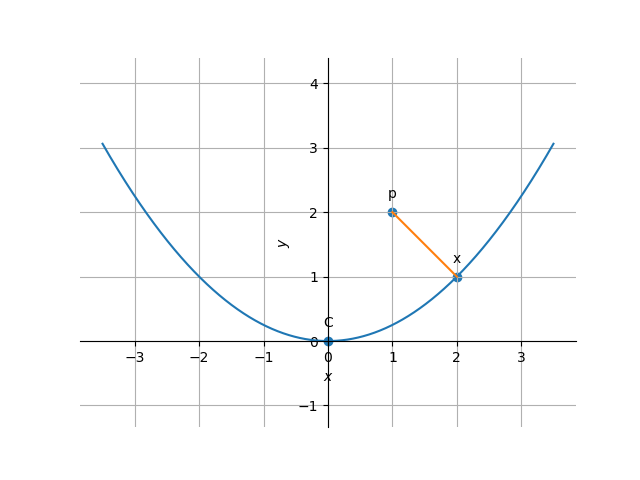
\includegraphics[scale=0.55]{opt.png}
\caption{The function f(x) with maxima and minima points}
\end{figure}        

\subsection{Calculation of Minima using gradient descent algorithm}
To find: 
\begin{align}
\min_{x} f(x)
\end{align}  
Given:
\begin{align}
f(x) = \cos^2x + \sin x,\quad x \in [0,\pi] 
\end{align}
\fi
The 
minima  is found by 
\begin{align}
	x_{n+1} &= x_n - \alpha \nabla f(x_n)
\\
 &= x_n - \alpha \brak{cosx_n-2sinx_ncosx_n}
\end{align}
\iffalse
where \\
1)$x_0=0.5$ \\
2)$\alpha=0.001$ \\
3)precision $= 0.00000001$ \\
values obtained using python are:
    \begin{align}
        \boxed{\text{Minima} = 1 }\\
        \boxed{\text{Minima Point} = 1.57}
    \end{align}

\end{document}
\fi


\end{enumerate}

	\end{enumerate}
\item
At what points in the interval (0,2$\pi$) does the function $\sin2x$ attain its maximum value.
\label{12/6/5/8/1}
%\iffalse
\documentclass[journal,10pt,twocolumn]{article}
\usepackage{graphicx, float}
\usepackage[margin=0.5in]{geometry}
\usepackage{amsmath, bm}
\usepackage{array}
\usepackage{booktabs}
\usepackage{mathtools}

\providecommand{\norm}[1]{\left\lVert#1\right\rVert}
\let\vec\mathbf
\newcommand{\myvec}[1]{\ensuremath{\begin{pmatrix}#1\end{pmatrix}}}
\newcommand{\mydet}[1]{\ensuremath{\begin{vmatrix}#1\end{vmatrix}}}

\title{\textbf{Optimization Assignment}}
\author{Maddu Dinesh}
\date{September 2022}

\begin{document}

\maketitle
\paragraph{\textit{Problem Statement} -
\fi
At what points in the interval (0,2$\pi$) does the function $\sin2x$ attain its maximum value.
\\
\solution
	\begin{figure}[!ht]
		\centering
		\includegraphics[width=\columnwidth]{12/6/5/8/figs/a.png}
		\caption{}
		\label{fig:12/6/5/8}
  	\end{figure}
\iffalse
\section*{\large Figure}

\begin{figure}[H]
\centering
\includegraphics[width=1\columnwidth]{a.png}
\caption{Graph of f(x)}
\label{fig:triangle}
\end{figure}
\section*{\large Solution}

	
    \subsection*{\normalsize Gradient descent}
\fi    
  Since  
    \begin{align}
	\label{eq:12/6/5/8vol_varx}
	    f(x) &= \sin2x,
	    \\
	    f'(x) &= 2\cos2x
	\end{align}
\iffalse
we have to attain the maximum value of sin2x in the interval [0,2$\pi$]. This can be seen in Figure f(x).
\fi
Using gradient ascent, 
\begin{align}
	x_{n+1} &= x_n + \alpha \nabla f(x_n) \\
&=x_n+\alpha(2\cos2x)
\end{align}
Choosing
\begin{align}
	x_0&=0.5,\alpha=0.001, precision = 0.00000001, 
	\\
	f_{max} &= 1.0000,
 	x_{max}= 0.7854.
    \end{align}
   
    

    





 







\item
Find the absolute maximum and minimum values of the function $f$ given by 
\begin{align}
	f(x) = \cos^2x + \sin x,\quad x \in \sbrak{0,\pi} 
\end{align} 
\label{12/6/6/14/1}
%\iffalse
\documentclass[10pt,twocolumn]{article}
\usepackage{graphicx}
\usepackage[margin=0.5in]{geometry}
\usepackage[cmex10]{amsmath}
\usepackage{array}
\usepackage{booktabs}
\usepackage{mathtools}
\title{\textbf{Optimization Assignment}}
\author{Sinkona Chinthamalla}

\providecommand{\norm}[1]{\lVert#1\rVert}
\providecommand{\abs}[1]{\vert#1\vert}
\let\vec\mathbf
\newcommand{\myvec}[1]{\ensuremath{\begin{pmatrix}#1\end{pmatrix}}}
\newcommand{\mydet}[1]{\ensuremath{\begin{vmatrix}#1\end{vmatrix}}}
\providecommand{\brak}[1]{\ensuremath{\left(#1\right)}}
\providecommand{\lbrak}[1]{\ensuremath{\left(#1\right.}}
\providecommand{\rbrak}[1]{\ensuremath{\left.#1\right)}}
\providecommand{\sbrak}[1]{\ensuremath{{}\left[#1\right]}}

\begin{document}

\maketitle
\paragraph{\textit{Problem Statement} -
\fi
Find the absolute maximum and minimum values of the function $f$ given by 
\begin{align}
	f(x) = \cos^2x + \sin x,\quad x \in \sbrak{0,\pi} 
\end{align} 
\solution
	\begin{figure}[!ht]
		\centering
		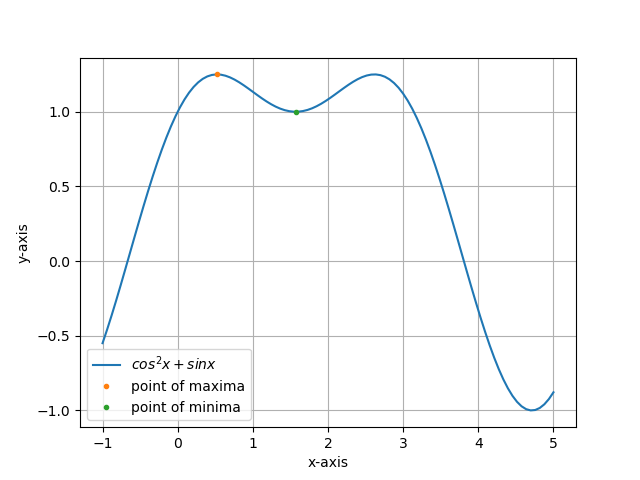
\includegraphics[width=\columnwidth]{12/6/6/14/figs/opt.png}
		\caption{}
		\label{fig:12/6/6/14}
  	\end{figure}
\iffalse

\section{Solution}
\begin{flushleft}
Given function is,\\
\end{flushleft}
\begin{equation}
    f(x)=\cos^2x + \sin x
\end{equation}
\subsection{Calculation using normal differentiation}
\begin{flushleft}
Differentiating (1) yields,
\end{flushleft}
\fi
The derivative of the given function is
\begin{align}
\nabla f(x) = \cos x-2\sin x \cos x 
\end{align}
\iffalse

\noindent Calculating the critical points:
$ \nabla f(x) = 0 $

\begin{equation}
\implies \cos{x} = 0 
\end{equation}
\begin{equation}
\implies -2\sin{x} + 1 = 0
\end{equation}
Therefore, the critical points are 

\begin{equation}
\frac{\pi}{6},\quad\frac{5\pi}{6},\quad\frac{\pi}{2}
\end{equation}

\textbf{1.1.1 Finding absolute maximum and minimum} 
Since given interval is $x \in [0,\pi]$ 

\begin{table}[h]
\centering
\large
\begin{tabular}{|l|l|}
\hline
\textbf{value of x} & \textbf{value of} \\ \hline
At x =0             & 1                 \\ \hline
At x =$ \frac{\pi}{6}$            & $\frac{5}{4}$            \\ \hline
At x =  $ \frac{\pi}{2}$            & 1                 \\ \hline
At x =  $ \frac{5\pi}{6}$            & $\frac{5}{4}$             \\ \hline
at x =       $\pi$       & 1                 \\ \hline
\end{tabular}
\end{table}

Hence, 
\begin{align}
\text{absolute maximum} & =  \frac{5}{4}\\
\text{absolute minimum} & = 1
\end{align}

\subsection{Calculation of Maxima using gradient ascent algorithm}
\fi
The 
maxima is calculated by
\begin{align}
x_{n+1} = x_n + \alpha \nabla f(x_n) 
\\
 &= x_n + \alpha \brak{cosx_n-2sinx_ncosx_n}
\end{align}
where 
\begin{enumerate}
	\item $x_0=0.5$ 
	\item $\alpha=0.001$ 
	\item precision $= 0.00000001$ 
\end{enumerate}
yielding
    \begin{align}
	    f_{max} = 1.25, 
 x_{max}        = 0.52.
    \end{align}
    \iffalse
    
\begin{figure}[h!]
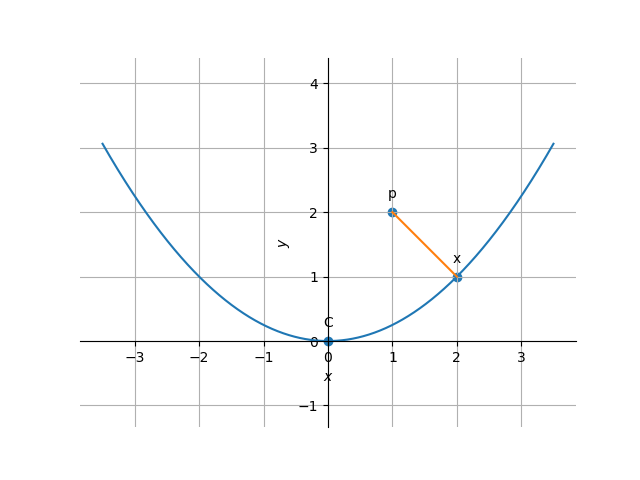
\includegraphics[scale=0.55]{opt.png}
\caption{The function f(x) with maxima and minima points}
\end{figure}        

\subsection{Calculation of Minima using gradient descent algorithm}
To find: 
\begin{align}
\min_{x} f(x)
\end{align}  
Given:
\begin{align}
f(x) = \cos^2x + \sin x,\quad x \in [0,\pi] 
\end{align}
\fi
The 
minima  is found by 
\begin{align}
	x_{n+1} &= x_n - \alpha \nabla f(x_n)
\\
 &= x_n - \alpha \brak{cosx_n-2sinx_ncosx_n}
\end{align}
\iffalse
where \\
1)$x_0=0.5$ \\
2)$\alpha=0.001$ \\
3)precision $= 0.00000001$ \\
values obtained using python are:
    \begin{align}
        \boxed{\text{Minima} = 1 }\\
        \boxed{\text{Minima Point} = 1.57}
    \end{align}

\end{document}
\fi

	\item Find the equation of the normal to the curve $x^2=4y$ and passing through the point $(1,2)$.
		\\
		\solution
\iffalse
\documentclass[12pt]{article}
\usepackage{graphicx}
\usepackage[none]{hyphenat}
\usepackage{graphicx}
\usepackage{listings}
\usepackage[english]{babel}
\usepackage{graphicx}
\usepackage{caption} 
\usepackage{booktabs}
\usepackage{array}
\usepackage{amssymb} % for \because
\usepackage{amsmath}   % for having text in math mode
\usepackage{extarrows} % for Row operations arrows
\usepackage{listings}
\lstset{
  frame=single,
  breaklines=true
}
\usepackage{hyperref}
  
%Following 2 lines were added to remove the blank page at the beginning
\usepackage{atbegshi}% http://ctan.org/pkg/atbegshi
\AtBeginDocument{\AtBeginShipoutNext{\AtBeginShipoutDiscard}}
\usepackage{gensymb}


%New macro definitions
\newcommand{\mydet}[1]{\ensuremath{\begin{vmatrix}#1\end{vmatrix}}}
\providecommand{\brak}[1]{\ensuremath{\left(#1\right)}}
\providecommand{\sbrak}[1]{\ensuremath{{}\left[#1\right]}}
\providecommand{\norm}[1]{\left\lVert#1\right\rVert}
\providecommand{\abs}[1]{\left\vert#1\right\vert}
\newcommand{\solution}{\noindent \textbf{Solution: }}
\newcommand{\myvec}[1]{\ensuremath{\begin{pmatrix}#1\end{pmatrix}}}
\let\vec\mathbf


\begin{document}

\begin{center}
	\title{\textbf{Quadratric Programming}}
\date{\vspace{-5ex}} %Not to print date automatically
\maketitle
\end{center}
\setcounter{page}{1}

\section{12$^{th}$ Maths - Chapter 6}
This is Problem-23 from Exercise 6.6 
\begin{enumerate}

\solution 
\fi
The given equation of the curve can be written as  
\begin{align}
	\label{eq:12/6/6/23/conv/parabolaEq2}
	g\brak{\vec{x}} = \vec{x}^T\vec{V}\vec{x} + 2\vec{u}^T\vec{x} + f = 0 
\end{align}
The given problem can be formulated as 
\begin{align}
	\label{eq:12/6/6/23/conv/Eq3}
	&  \min_{\vec{x}} \quad \text{f}\brak{\vec{x}} = \norm{\vec{x}-\vec{h}}^2\\
	\label{eq:12/6/6/23/conv/Eq4}
	& \text{s.t.}\quad g\brak{\vec{x}} = \vec{x}^T\vec{V}\vec{x} + 2\vec{u}^T\vec{x} + f = 0  
\end{align}
where
\begin{align}
	\vec{V} = \myvec{ 1 & 0 \\ 0 & 0},\,
	\vec{u} = \myvec{0 \\ -2},\, 
	f = 0,\,
	\vec{h} = \myvec{1 \\ 2}
\end{align}
The optimization problem is nonconvex. However, by relaxing the constraint in \eqref{eq:12/6/6/23/conv/Eq4} as
\begin{align}
	\label{eq:12/6/6/23/conv/Eq7}
	& g\brak{\vec{x}} = \vec{x}^T\vec{V}\vec{x} + 2\vec{u}^T\vec{x} + f \le 0  
\end{align}
the optimization problem can be made convex. Using cvxpy, input the objective function, contraints and solve. However, resultant optimal point is the given point itself. This is because, the point is inside the parabola. Looks like, this is a limitation of cvxpy.


\end{enumerate}

\section{Nonconvex Examples}
\begin{enumerate}[label=\thechapter.\arabic*,ref=\thechapter.\theenumi]
\numberwithin{equation}{enumi}
\numberwithin{figure}{enumi}
\numberwithin{table}{enumi}
 \item The point on the curve 
    \begin{align}
        x^2 = 2y
        \label{eq:12/6/5/27/curve}
    \end{align}
    which is nearest to the point 
    $\vec{P} = \myvec{0\\5}$ is
    \begin{enumerate}
        \item $\myvec{2\sqrt{2}\\4}$
        \item $\myvec{2\sqrt{2}\\0}$
        \item $\myvec{0\\0}$
        \item $\myvec{2\\2}$
    \end{enumerate}
\solution 
\label{12/6/5/27/nonconv/nonconv}
\iffalse
\documentclass[journal,12pt,twocolumn]{IEEEtran}
\usepackage{setspace}
\usepackage{gensymb}
\usepackage{xcolor}
\usepackage{caption}
\singlespacing
\usepackage{siunitx}
\usepackage[cmex10]{amsmath}
\usepackage{mathtools}
\usepackage{hyperref}
\usepackage{amsthm}
\usepackage{mathrsfs}
\usepackage{txfonts}
\usepackage{stfloats}
\usepackage{cite}
\usepackage{cases}
\usepackage{subfig}
\usepackage{longtable}
\usepackage{multirow}
\usepackage{enumitem}
\usepackage{bm}
\usepackage{mathtools}
\usepackage{listings}
\usepackage{tikz}
\usetikzlibrary{shapes,arrows,positioning}
\usepackage{circuitikz}
\renewcommand{\vec}[1]{\boldsymbol{\mathbf{#1}}}
\DeclareMathOperator*{\Res}{Res}
\renewcommand\thesection{\arabic{section}}
\renewcommand\thesubsection{\thesection.\arabic{subsection}}
\renewcommand\thesubsubsection{\thesubsection.\arabic{subsubsection}}

\renewcommand\thesectiondis{\arabic{section}}
\renewcommand\thesubsectiondis{\thesectiondis.\arabic{subsection}}
\renewcommand\thesubsubsectiondis{\thesubsectiondis.\arabic{subsubsection}}
\hyphenation{op-tical net-works semi-conduc-tor}

\lstset{
language=Python,
frame=single, 
breaklines=true,
columns=fullflexible
}
\begin{document}
\theoremstyle{definition}
\newtheorem{theorem}{Theorem}[section]
\newtheorem{problem}{Problem}
\newtheorem{proposition}{Proposition}[section]
\newtheorem{lemma}{Lemma}[section]
\newtheorem{corollary}[theorem]{Corollary}
\newtheorem{example}{Example}[section]
\newtheorem{definition}{Definition}[section]
\newcommand{\BEQA}{\begin{eqnarray}}
\newcommand{\EEQA}{\end{eqnarray}}
\newcommand{\define}{\stackrel{\triangle}{=}}
\newcommand{\myvec}[1]{\ensuremath{\begin{pmatrix}#1\end{pmatrix}}}
\newcommand{\mydet}[1]{\ensuremath{\begin{vmatrix}#1\end{vmatrix}}}
\bibliographystyle{IEEEtran}
\providecommand{\nCr}[2]{\,^{#1}C_{#2}} % nCr
\providecommand{\nPr}[2]{\,^{#1}P_{#2}} % nPr
\providecommand{\mbf}{\mathbf}
\providecommand{\pr}[1]{\ensuremath{\Pr\left(#1\right)}}
\providecommand{\qfunc}[1]{\ensuremath{Q\left(#1\right)}}
\providecommand{\sbrak}[1]{\ensuremath{{}\left[#1\right]}}
\providecommand{\lsbrak}[1]{\ensuremath{{}\left[#1\right.}}
\providecommand{\rsbrak}[1]{\ensuremath{{}\left.#1\right]}}
\providecommand{\brak}[1]{\ensuremath{\left(#1\right)}}
\providecommand{\lbrak}[1]{\ensuremath{\left(#1\right.}}
\providecommand{\rbrak}[1]{\ensuremath{\left.#1\right)}}
\providecommand{\cbrak}[1]{\ensuremath{\left\{#1\right\}}}
\providecommand{\lcbrak}[1]{\ensuremath{\left\{#1\right.}}
\providecommand{\rcbrak}[1]{\ensuremath{\left.#1\right\}}}
\theoremstyle{remark}
\newtheorem{rem}{Remark}
\newcommand{\sgn}{\mathop{\mathrm{sgn}}}
\newcommand{\rect}{\mathop{\mathrm{rect}}}
\newcommand{\sinc}{\mathop{\mathrm{sinc}}}
\providecommand{\abs}[1]{\left\vert#1\right\vert}
\providecommand{\res}[1]{\Res\displaylimits_{#1}} 
\providecommand{\norm}[1]{\left\Vert#1\right\Vert}
\providecommand{\mtx}[1]{\mathbf{#1}}
\providecommand{\mean}[1]{E\left[ #1 \right]}
\providecommand{\fourier}{\overset{\mathcal{F}}{ \rightleftharpoons}}
\providecommand{\ztrans}{\overset{\mathcal{Z}}{ \rightleftharpoons}}
\providecommand{\system}[1]{\overset{\mathcal{#1}}{ \longleftrightarrow}}
\newcommand{\solution}{\noindent \textbf{Solution: }}
\providecommand{\dec}[2]{\ensuremath{\overset{#1}{\underset{#2}{\gtrless}}}}
\let\StandardTheFigure\thefigure
\def\putbox#1#2#3{\makebox[0in][l]{\makebox[#1][l]{}\raisebox{\baselineskip}[0in][0in]{\raisebox{#2}[0in][0in]{#3}}}}
     \def\rightbox#1{\makebox[0in][r]{#1}}
     \def\centbox#1{\makebox[0in]{#1}}
     \def\topbox#1{\raisebox{-\baselineskip}[0in][0in]{#1}}
     \def\midbox#1{\raisebox{-0.5\baselineskip}[0in][0in]{#1}}

\vspace{3cm}
\title{Quadratic Programming Assignment}
\author{Gautam Singh}
\maketitle
\bigskip

\begin{abstract}
    This document contains the solution to Question 27 of Exercise 5 in Chapter
    6 of the class 12 NCERT textbook.
\end{abstract}

\begin{enumerate}
    \item Show that the point on the curve 
    \begin{align}
        x^2 = 2y
        \label{eq:12/6/5/27/nonconv/nonconv/curve}
    \end{align}
    which is nearest to the point $\vec{P} = \myvec{0\\5}$ is a nonconvex
    optimization problem.

    \solution 
    \fi
		We need to find
    \begin{align}
        \min_{\vec{x}} g\brak{\vec{x}} &= \norm{\vec{x}-\vec{P}}^2 \label{eq:12/6/5/27/nonconv/nonconv/cost} \\
        \textrm{s.t. } h\brak{\vec{x}} &= \vec{x}^\top\vec{Vx} + 2\vec{u}^\top\vec{x} + f = 0 \label{eq:12/6/5/27/nonconv/nonconv/constr}
    \end{align}
    where
    \begin{align}
        \vec{V} = \myvec{1&0\\0&0},\ \vec{u} = \myvec{0\\-1},\ f = 0
    \end{align}
    Suppose $\vec{x_1}$ and $\vec{x_2}$ satisfy $h\brak{\vec{x}} = 0$. Then, 
    \begin{align}
        \vec{x_1}^\top\vec{Vx_1} + 2\vec{u}^\top\vec{x_1} + f &= 0 \label{eq:12/6/5/27/nonconv/nonconv/x1-parab} \\
        \vec{x_2}^\top\vec{Vx_2} + 2\vec{u}^\top\vec{x_2} + f &= 0 \label{eq:12/6/5/27/nonconv/nonconv/x2-parab}
    \end{align}
    Then, for any $0 \le \lambda \le 1$, substituting
    \begin{align}
        \vec{x} =\lambda\vec{x_1} + \brak{1-\lambda}\vec{x_2}
    \end{align}
    into \eqref{eq:12/6/5/27/nonconv/nonconv/constr}, we get
    \begin{align}
        h\brak{\vec{x}} = \lambda\brak{\lambda-1}\brak{\vec{x_1}-\vec{x_2}}^\top\vec{V}\brak{\vec{x_1}-\vec{x_2}} \neq 0
        \label{eq:12/6/5/27/nonconv/nonconv/nonconvex}
    \end{align}
    since $\vec{x_1} - \vec{x_2}$ can be arbitrary.  Hence, the optimization 
    problem is nonconvex as the set of points on the parabola do not form a 
    convex set. The constraints throw an error when \textit{cvxpy} is used. 
    

\end{enumerate}

\chapter{Gradient Descent}
\section{Definition}
\renewcommand{\theequation}{\theenumi}
\begin{enumerate}[label=\thesection.\arabic*.,ref=\thesection.\theenumi]
\numberwithin{equation}{enumi}
%\item Consider the problem of finding the square root of a number $c$.  This can be expressed as the equation
%%
%\begin{equation}
%\label{eq:root}
%x^2 -c= 0
%\end{equation}
%%
%
%\item
%Sketch the function for different values of $c$
%%
%\begin{equation}
%f(x)= x^{3}-3xc
%\end{equation}
%%
%and comment upon its convexity.
%
%\item
%Show that \eqref{eq:root} results from
%\begin{align}
%\min_{x}f(x)= x^{3}-3xc
%\end{align}

\item
Find a numerical solution for \eqref{eq:opt_line_dist_uncon}

\eqref{eq:opt_line_dist_uncon}

%
%\begin{align}
%f(\lambda) = a\lambda^2 + b\lambda + d
%\end{align}
%
%\eqref{eq:root}.
%\\
\solution
A numerical solution for \eqref{eq:opt_line_dist_uncon} is obtained as
%
\begin{align}
\lambda_{n+1}&=\lambda_{n}-\mu f^{\prime}\brak{\lambda_n}
\\
&=\lambda_{n} -\mu \brak{2a\lambda_n+b}
\label{eq:opt/grad_des/gradient}
\end{align}

%\begin{align}
%x_{n+1}&=x_{n}-{\frac {f(x_{n})}{f^{\prime}(x_{n})}}
%\\
%&=x_{n} -\frac{x^2_{n}-c}{2x_n} 
%\\
%&=\frac{1}{2}\sbrak{x_{n} +\frac{c}{x_n} }
%\label{eq:newton}
%\end{align}
%
where $\lambda_0$ is an inital guess and $\mu$ is a variable parameter. The choice of these parameters is very important since they decide how fast the algorithm converges.
%
\item
Write a program to implement \eqref{eq:opt/grad_des/gradient}.
%
\\
\solution Download and execute
\begin{lstlisting}
opt/codes/gd.py
\end{lstlisting}
%
\item Find a closed form solution for $\lambda_n$ in  \eqref{eq:opt/grad_des/gradient} using the one sided Z transform.
%
\item Find the condition for which \eqref{eq:opt/grad_des/gradient} converges, i.e.
\begin{align}
\lim_{n \to \infty}\abs{\lambda_{n+1}-\lambda_n} = 0
\end{align}
\end{enumerate}


\section{Examples}
\begin{enumerate}[label=\thechapter.\arabic*,ref=\thechapter.\theenumi]
\numberwithin{equation}{enumi}
\numberwithin{figure}{enumi}
\numberwithin{table}{enumi}
\item  Reduce the equation $y-2=0$ into normal form. Find the perpendicular distances from the origin and angle between perpendicular and the positive x-axis.
	\\
\solution 
\label{11/10/3/3/2/grad}
\iffalse

\documentclass[12pt]{article}
\usepackage{graphicx}
\usepackage{amsmath}
\usepackage{mathtools}
\usepackage{gensymb}
\usepackage{tabularx}
\usepackage{array}
\usepackage[latin1]{inputenc}
\usepackage{fullpage}
\usepackage{color}
\usepackage{array}
\usepackage{longtable}
\usepackage{calc}
\usepackage{multirow}
\usepackage{hhline}
\usepackage{ifthen}
\usepackage{lscape}
\usepackage{float}
\usepackage{amssymb}

\newcommand{\mydet}[1]{\ensuremath{\begin{vmatrix}#1\end{vmatrix}}}
\providecommand{\brak}[1]{\ensuremath{\left(#1\right)}}
\providecommand{\cbrak}[1]{\ensuremath{\left\{#1\right\}}}
\providecommand{\norm}[1]{\left\lVert#1\right\rVert}
\providecommand{\abs}[1]{\left\vert#1\right\vert}
\newcommand{\solution}{\noindent \textbf{Solution: }}
\newcommand{\myvec}[1]{\ensuremath{\begin{pmatrix}#1\end{pmatrix}}}
\let\vec\mathbf

\def\inputGnumericTable{}

\begin{document}
\begin{center}
\textbf\large{OPTIMIZATION}

\end{center}
\section*{Excercise 10.3}


\solution
\fi
The given equation can be represented in parametric form as
\begin{align}
	\label{eq:11/10/3/3/2/grad/eq2}
	\vec{x} = \vec{A}+\lambda\vec{m}
\end{align}
where
\begin{align}
	\vec{A} = \myvec{2\\2}, \vec{m} = \myvec{1\\0}
	\label{eq:11/10/3/3/2/grad/line}
\end{align}
Let $\vec{O}$ be the origin. The perpendicular distance will be the minimum distance from $\vec{O}$ to the line. Let $\vec{P}$ be the foot of perpendicular. This problem can be formulated as an optimization problem as follows:
\begin{align}
	d_{\min} &= 	 \min_{\vec{x}}\norm{\vec{x}-\vec{O}}^2\\
	 &= \min_{\lambda}\norm{\vec{A}+\lambda\vec{m}-\vec{O}}^2\\
	&= \norm{\vec{m}}^2\lambda^2+2\lambda\vec{A}^\top\vec{m}+\norm{\vec{A}}^2
	\label{eq:11/10/3/3/2/grad/eq3}
	\\
	&= \lambda^2+4\lambda+8 = f^\prime\brak{\lambda} 
	\label{eq:11/10/3/3/2/grad/eq4}
\end{align}
upon substituting numerical values.
$\because$ the coefficient of $\lambda^2>0$, \eqref{eq:11/10/3/3/2/grad/eq3} is a convex function
The update equation using Gradient Descent is
\begin{align}
	\lambda_{n+1} &= \lambda_n - \alpha\nabla f\brak{\lambda_n}\\
	\label{eq:11/10/3/3/2/grad/eq5}
 &= \brak{1-2\alpha}\lambda_{n} - 4\alpha
\end{align}
Taking one-sided Z-transform on both sides of \eqref{eq:11/10/3/3/2/grad/eq5},
\begin{align}
	z\Lambda\brak{z} &= \brak{1-2\alpha}\Lambda\brak{z} - \frac{4\alpha}{1-z^{-1}}\\
	\Lambda\brak{z} &= -\frac{4\alpha z^{-1}}{\brak{1-\brak{1-2\alpha}z^{-1}}\brak{1-z^{-1}}}\\
	&= 2\brak{\frac{1}{\brak{1-\brak{1-2\alpha}z^{-1}}}-\frac{1}{1-z^{-1}}}\\
	\label{eq:11/10/3/3/2/grad/eq6}
	&= 2\sum_{k=0}^{\infty}\brak{\brak{1-2\alpha}^{k}-1}z^{-k}
\end{align}
from \eqref{eq:11/10/3/3/2/grad/eq6}, the ROC is
\begin{align}
	\abs{z}>\max\cbrak{{1,\abs{1-2\alpha}}}\\
	\implies 0<\abs{1-2\alpha}<1\\
	\label{eq:11/10/3/3/2/grad/eq7}
	\implies 0<\alpha<\frac{1}{2}
\end{align}
Thus, if $\alpha$ satisfies \eqref{eq:11/10/3/3/2/grad/eq7}, then from \eqref{eq:11/10/3/3/2/grad/eq6}
\begin{align}
	\lim_{n\to\infty} \lambda_{n} = -2
\end{align}
Choosing
\begin{enumerate}
\item $\alpha$ = 0.001
\item precision = 0.0000001
\item n = 10000000
\item $\lambda_0$ = 4
\begin{align}
	\lambda_{min} = -2
\end{align}
\end{enumerate}
\begin{align}
	\vec{x}_{min} &= \vec{P} = \myvec{2\\2}+\brak{-2}\myvec{1\\0}\\
	&= \myvec{0\\2}\\
	OP &= \norm{\vec{P}-\vec{O}}\\
	&= \norm{\myvec{0\\2}-\myvec{0\\0}}\\
	&= 2
\end{align}
See Fig. \ref{fig:11/10/3/3/2/grad/Fig1} and Fig. \ref{fig:11/10/3/3/2/grad/Fig2}
\begin{figure}[!h]
	\begin{center} 
	    \includegraphics[width=\columnwidth]{11/10/3/3/2/grad/figs/opt1}
	\end{center}
\caption{}
\label{fig:11/10/3/3/2/grad/Fig1}
\end{figure}
\begin{figure}[!h]
	\begin{center} 
	    \includegraphics[width=\columnwidth]{11/10/3/3/2/grad/figs/opt2}
	\end{center}
\caption{}
\label{fig:11/10/3/3/2/grad/Fig2}
\end{figure}

	\\
\item Reduce $x-\sqrt{3}y+8=0$ into normal form. Find its perpendicular distance from the origin and angle between perpendicular and the positive x-axis. 
	\\
\solution 
\label{11/10/3/3/1/grad}
\iffalse
\documentclass[12pt]{article}
\usepackage{graphicx}
\usepackage[none]{hyphenat}
\usepackage{graphicx}
\usepackage{listings}
\usepackage[english]{babel}
\usepackage{graphicx}
\usepackage{caption} 
\usepackage{booktabs}
\usepackage{array}
\usepackage{amsmath}   % for having text in math mode
\usepackage{amssymb} % for \because
\usepackage{extarrows} % for Row operations arrows
\usepackage{listings}
\lstset{
  frame=single,
  breaklines=true
}
\usepackage{hyperref}
  
%Following 2 lines were added to remove the blank page at the beginning
\usepackage{atbegshi}% http://ctan.org/pkg/atbegshi
\AtBeginDocument{\AtBeginShipoutNext{\AtBeginShipoutDiscard}}
\usepackage{gensymb}


%New macro definitions
\newcommand{\mydet}[1]{\ensuremath{\begin{vmatrix}#1\end{vmatrix}}}
\providecommand{\brak}[1]{\ensuremath{\left(#1\right)}}
\providecommand{\sbrak}[1]{\ensuremath{{}\left[#1\right]}}
\providecommand{\norm}[1]{\left\lVert#1\right\rVert}
\providecommand{\cbrak}[1]{\ensuremath{\left\{#1\right\}}}
\providecommand{\abs}[1]{\left\vert#1\right\vert}
\newcommand{\solution}{\noindent \textbf{Solution: }}
\newcommand{\myvec}[1]{\ensuremath{\begin{pmatrix}#1\end{pmatrix}}}
\let\vec\mathbf


\begin{document}

\begin{center}
\title{\textbf{Gradient Descent}}
\date{\vspace{-5ex}} %Not to print date automatically
\maketitle
\end{center}
\setcounter{page}{1}

\section{11$^{th}$ Maths - Chapter 10}
This is Problem-3.1 from Exercise 10.3 
\begin{enumerate}

\solution 
\fi
The given line  can be represented in parametric form as
\begin{align}
	\label{eq:11/10/3/3/1/grad/Eq2}
	\vec{x} = \vec{A}+\lambda\vec{m}
\end{align}
where
\begin{align}
	\vec{A} &= \myvec{-8 \\ 0}\\
	\vec{O} &= \myvec{ 0 \\ 0} \\
	\vec{m} &= \myvec{1 \\ \frac{1}{\sqrt{3}}} \\
\end{align}
 yielding 
\begin{align}
\label{eq:11/10/3/3/1/grad/Eq6}
	f\brak{\lambda} &= \frac{4}{3}\lambda^2-16\lambda+64 \\ 
	f^\prime\brak{\lambda} &= \frac{8}{3}\lambda - 16
\end{align}
Computing $\lambda_{min}$ using Gradient Descent method:
\begin{align}
	\lambda_{n+1} &= \lambda_n - \alpha f^\prime\brak{\lambda_n}\\
	\label{eq:11/10/3/3/1/grad/grad_des}
	\lambda_{n+1} &= \lambda_n\brak{1-\frac{8}{3}\alpha} + 16\alpha
\end{align}
Taking the one-sided $Z$-transform on both sides of \eqref{eq:11/10/3/3/1/grad/grad_des},
\begin{align}
            \label{eq:11/10/3/3/1/grad/Z-trans-eqn}
	    z\Lambda\brak{z} &= \brak{1-\frac{8}{3}\alpha}\Lambda\brak{z} + \frac{16\alpha}{1-z^{-1}} \\
	    \Lambda\brak{z} &= \frac{16\alpha z^{-1}}{\brak{1-z^{-1}}\brak{1-\brak{1-\frac{8}{8}\alpha}z^{-1}}} \\
	    &= 6\brak{ \frac{1}{1-z^{-1}} - \frac{1}{1-\brak{1-\frac{8}{3}\alpha}z^{-1}}} \\
            \label{eq:11/10/3/3/1/grad/lambda-z-trans}
	    &= 6\sum_{k=0}^{\infty}\brak{1-\brak{1-\frac{8}{3}\alpha}^k}z^{-k}
\end{align}
From \eqref{eq:11/10/3/3/1/grad/lambda-z-trans}, the ROC is
\begin{align}
	\abs{z} &> \max\cbrak{1,\abs{1-\frac{8}{3}\alpha}} \\
	\implies -1 & < \abs{1-\frac{8}{3}\alpha} < 1 \\
        \label{eq:11/10/3/3/1/grad/alpha-constr}
        \implies 0 &< \alpha < \frac{3}{4}
\end{align}
Thus, if $\alpha$ satisfies \eqref{eq:11/10/3/3/1/grad/alpha-constr}, then from \eqref{eq:11/10/3/3/1/grad/lambda-z-trans}, 
\begin{align}
	\label{eq:11/10/3/3/1/grad/conv}
        \lim_{n\to\infty}\lambda_n &= 6 
    \end{align}
Choosing
\begin{enumerate}
 \item $\alpha$ = 0.001
 \item precision = 0.0000001
 \item n = 10000000 
 \item $\lambda_0$ = -5 
\end{enumerate}
\begin{align}
	\lambda_{min} &= 6 
\end{align}
Substituting the values of $\vec{A}$, $\vec{m}$ and $\lambda_{min}$ in equation \eqref{eq:11/10/3/3/1/grad/Eq2} 
\begin{align}
	\vec{x}_{min} &= \vec{P} = \myvec{-8 \\ 0}+6\myvec{1 \\ \frac{1}{\sqrt{3}}}  \\
	&= \myvec{-8 \\ 0}+\myvec{6 \\ \frac{6}{\sqrt{3}}} \\
	&= \myvec{-2 \\ 2\sqrt{3}} \\
	OP &= \norm{\vec{P}-\vec{O}}^2 \\ 
	&= \norm{\myvec{-2 \\ 2\sqrt{3}}-\myvec{0 \\ 0}} \\
	&= \sqrt{2^2 + 12} = \sqrt{16} = 4
\end{align}
See Figs. \ref{fig:11/10/3/3/1/grad/Fig1} and \ref{fig:11/10/3/3/1/grad/Fig2}.
\begin{figure}[!h]
	\begin{center}
		\includegraphics[width=\columnwidth]{11/10/3/3/1/grad/figs/problem3.1a.pdf}
	\end{center}
\caption{}
\label{fig:11/10/3/3/1/grad/Fig1}
\end{figure}
\begin{figure}[!h]
	\begin{center}
		\includegraphics[width=\columnwidth]{11/10/3/3/1/grad/figs/problem3.1b.pdf}
	\end{center}
\caption{}
\label{fig:11/10/3/3/1/grad/Fig2}
\end{figure}

  \item Find the coordinates of the foot of perpendicular from the point 
    \begin{align}
        \vec{P} = \myvec{-1\\3}
        \label{eq:11/10/3/14/grad/P-def}
    \end{align}
    to the line 
    \begin{align}
        \myvec{3&-4}\vec{x} = 16
        \label{eq:11/10/3/14/grad/line}
    \end{align}
\solution 
\label{11/10/3/14/grad}
\iffalse
\documentclass[journal,12pt,twocolumn]{IEEEtran}
\usepackage{setspace}
\usepackage{gensymb}
\singlespacing
\usepackage[cmex10]{amsmath}
\usepackage{amsthm}
\usepackage{mathrsfs}
\usepackage{txfonts}
\usepackage{stfloats}
\usepackage{bm}
\usepackage{cite}
\usepackage{cases}
\usepackage{subfig}
\usepackage{longtable}
\usepackage{multirow}
\usepackage{enumitem}
\usepackage{mathtools}
\usepackage{tikz}
\usepackage{circuitikz}
\usepackage{verbatim}
\usepackage[breaklinks=true]{hyperref}
\usepackage{tkz-euclide} % loads  TikZ and tkz-base
\usepackage{listings}
\usepackage{color}    
\usepackage{array}    
\usepackage{longtable}
\usepackage{calc}     
\usepackage{multirow} 
\usepackage{hhline}   
\usepackage{ifthen}   
\usepackage{lscape}     
\usepackage{chngcntr}
\DeclareMathOperator*{\Res}{Res}
\renewcommand\thesection{\arabic{section}}
\renewcommand\thesubsection{\thesection.\arabic{subsection}}
\renewcommand\thesubsubsection{\thesubsection.\arabic{subsubsection}}

\renewcommand\thesectiondis{\arabic{section}}
\renewcommand\thesubsectiondis{\thesectiondis.\arabic{subsection}}
\renewcommand\thesubsubsectiondis{\thesubsectiondis.\arabic{subsubsection}}
\renewcommand\thetable{\arabic{table}}
% correct bad hyphenation here
\hyphenation{op-tical net-works semi-conduc-tor}
\def\inputGnumericTable{}                                 %%

\lstset{
%language=C,
frame=single, 
breaklines=true,
columns=fullflexible
}
%\lstset{
%language=tex,
%frame=single, 
%breaklines=true
%}

\begin{document}
\newtheorem{theorem}{Theorem}[section]
\newtheorem{problem}{Problem}
\newtheorem{proposition}{Proposition}[section]
\newtheorem{lemma}{Lemma}[section]
\newtheorem{corollary}[theorem]{Corollary}
\newtheorem{example}{Example}[section]
\newtheorem{definition}[problem]{Definition}
\newcommand{\BEQA}{\begin{eqnarray}}
\newcommand{\EEQA}{\end{eqnarray}}
\newcommand{\define}{\stackrel{\triangle}{=}}
\bibliographystyle{IEEEtran}
\providecommand{\mbf}{\mathbf}
\providecommand{\pr}[1]{\ensuremath{\Pr\left(#1\right)}}
\providecommand{\qfunc}[1]{\ensuremath{Q\left(#1\right)}}
\providecommand{\sbrak}[1]{\ensuremath{{}\left[#1\right]}}
\providecommand{\lsbrak}[1]{\ensuremath{{}\left[#1\right.}}
\providecommand{\rsbrak}[1]{\ensuremath{{}\left.#1\right]}}
\providecommand{\brak}[1]{\ensuremath{\left(#1\right)}}
\providecommand{\lbrak}[1]{\ensuremath{\left(#1\right.}}
\providecommand{\rbrak}[1]{\ensuremath{\left.#1\right)}}
\providecommand{\cbrak}[1]{\ensuremath{\left\{#1\right\}}}
\providecommand{\lcbrak}[1]{\ensuremath{\left\{#1\right.}}
\providecommand{\rcbrak}[1]{\ensuremath{\left.#1\right\}}}
\theoremstyle{remark}
\newtheorem{rem}{Remark}
\newcommand{\sgn}{\mathop{\mathrm{sgn}}}
\providecommand{\abs}[1]{\left\vert#1\right\vert}
\providecommand{\res}[1]{\Res\displaylimits_{#1}} 
\providecommand{\norm}[1]{\left\lVert#1\right\rVert}
\providecommand{\mtx}[1]{\mathbf{#1}}
\providecommand{\mean}[1]{E\left[ #1 \right]}
\providecommand{\fourier}{\overset{\mathcal{F}}{ \rightleftharpoons}}
\providecommand{\system}[1]{\overset{\mathcal{#1}}{ \longleftrightarrow}}
\newcommand{\solution}{\noindent \textbf{Solution: }}
\newcommand{\cosec}{\,\text{cosec}\,}
\providecommand{\dec}[2]{\ensuremath{\overset{#1}{\underset{#2}{\gtrless}}}}
\newcommand{\myvec}[1]{\ensuremath{\begin{pmatrix}#1\end{pmatrix}}}
\newcommand{\mydet}[1]{\ensuremath{\begin{vmatrix}#1\end{vmatrix}}}
\let\vec\mathbf
\def\putbox#1#2#3{\makebox[0in][l]{\makebox[#1][l]{}\raisebox{\baselineskip}[0in][0in]{\raisebox{#2}[0in][0in]{#3}}}}
     \def\rightbox#1{\makebox[0in][r]{#1}}
     \def\centbox#1{\makebox[0in]{#1}}
     \def\topbox#1{\raisebox{-\baselineskip}[0in][0in]{#1}}
     \def\midbox#1{\raisebox{-0.5\baselineskip}[0in][0in]{#1}}

\vspace{3cm}
\title{Optimization Assignment}
\author{Gautam Singh}
\maketitle
\bigskip

\begin{abstract}
    This document contains the solution to Question 4 of Exercise 2 in Chapter
    10 of the class 11 NCERT textbook.
\end{abstract}

\begin{enumerate}
  
    \solution 
\fi
		Any point on \eqref{eq:11/10/3/14/grad/line} is clearly of the form
    \begin{align}
        \vec{Q} = \vec{A} + \lambda\vec{m}
        \label{eq:11/10/3/14/grad/Q-def}
    \end{align}
    where $\lambda \in \mathbb{R}$ and
    \begin{align}
        \vec{A} = \myvec{0\\-4},\ \vec{m} = \myvec{4\\3}
        \label{eq:11/10/3/14/grad/vals}
    \end{align}
    Thus,
    \begin{align}
        f\brak{\lambda} &= \norm{\vec{Q}-\vec{P}}^2 \\
                        &= \norm{\vec{A}-\vec{P}+\lambda\vec{m}}^2 \\
                        &= \norm{\vec{m}}^2\lambda^2 + 2\vec{m}^\top\brak{\vec{A}-\vec{P}}\lambda + \norm{\vec{A}-\vec{P}}^2
                        \label{eq:11/10/3/14/grad/dist-lambda}
    \end{align}
    Since \eqref{eq:11/10/3/14/grad/dist-lambda} is convex, we use the gradient descent function 
    on $\lambda$ to converge at the minimum of $f\brak{\lambda}$.
    \begin{align}
        \lambda_{n+1} &= \lambda_n - \alpha f'\brak{\lambda_n} \\
                      &= \brak{1-2\alpha\norm{\vec{m}}^2}\lambda_n + 2\alpha\vec{m}^\top\brak{\vec{A}-\vec{P}}
                      \label{eq:11/10/3/14/grad/diff-eqn}
    \end{align}
    Taking the one-sided $Z$-transform on both sides of \eqref{eq:11/10/3/14/grad/diff-eqn},
    \begin{align}
        z\Lambda\brak{z} &= \brak{1-2\alpha\norm{\vec{m}}^2}\Lambda\brak{z} - \frac{2\alpha\vec{m}^\top\brak{\vec{A}-\vec{P}}}{1-z^{-1}}
        \label{eq:11/10/3/14/grad/Z-trans-eqn}
    \end{align}
    Solving \eqref{eq:11/10/3/14/grad/Z-trans-eqn}
    \begin{align}
        &\Lambda\brak{z} = -\frac{2\alpha\vec{m}^\top\brak{\vec{A}-\vec{P}}z^{-1}}{\brak{1- z^{-1}}\brak{1 - \brak{1-2\alpha\norm{\vec{m}}^2}z^{-1}}} \label{eq:11/10/3/14/grad/roc} \\
        &= -\frac{\vec{m}^\top\brak{\vec{A}-\vec{P}}}{\norm{\vec{m}}^2}\lbrak{\frac{1}{1-z^{-1}}} \\
        &\rbrak{- \frac{1}{1-\brak{1-2\alpha\norm{\vec{m}}^2}z^{-1}}} \\
        &= \frac{\vec{m}^\top\brak{\vec{A}-\vec{P}}}{\norm{\vec{m}}^2}\sum_{k=0}^{\infty}\brak{1-\brak{1-2\alpha\norm{\vec{m}}^2}^k}z^{-k}
        \label{eq:11/10/3/14/grad/lambda-z-trans}
    \end{align}
    From \eqref{eq:11/10/3/14/grad/roc}, the ROC is
    \begin{align}
        \abs{z} &> \max\cbrak{1,1-2\alpha\norm{\vec{m}}^2} \\
        \implies 0 &< 1 - 2\alpha\norm{\vec{m}}^2 < 1 \\
        \implies 0 &< \alpha < \frac{1}{2\norm{\vec{m}}^2}
        \label{eq:11/10/3/14/grad/alpha-constr}
    \end{align}
    Thus, if $\alpha$ satisfies \eqref{eq:11/10/3/14/grad/alpha-constr}, then from 
    \eqref{eq:11/10/3/14/grad/lambda-z-trans}, substituting from \eqref{eq:11/10/3/14/grad/vals},
    \begin{align}
        \lim_{n\to\infty}\lambda_n &= -\frac{\vec{m}^\top\brak{\vec{A}-\vec{P}}}{\norm{\vec{m}^2}}                                  \label{eq:11/10/3/14/grad/conv}
                                   &= \frac{17}{25}
    \end{align}
    We select the following parameters to arrive at the optimal $\lambda$,
    where $N$ is the number of iterations and $\epsilon$ is the convergence 
    limit. The gradient descent is demonstrated in Fig. \ref{fig:11/10/3/14/grad/grad-desc},
    plotted by the Python code. The relevant
    parameters are shown in Table \ref{tab:11/10/3/14/grad/param}.
    \begin{table}[!ht]
        \centering
        %%%%%%%%%%%%%%%%%%%%%%%%%%%%%%%%%%%%%%%%%%%%%%%%%%%%%%%%%%%%%%%%%%%%%%
%%                                                                  %%
%%  This is the header of a LaTeX2e file exported from Gnumeric.    %%
%%                                                                  %%
%%  This file can be compiled as it stands or included in another   %%
%%  LaTeX document. The table is based on the longtable package so  %%
%%  the longtable options (headers, footers...) can be set in the   %%
%%  preamble section below (see PRAMBLE).                           %%
%%                                                                  %%
%%  To include the file in another, the following two lines must be %%
%%  in the including file:                                          %%
%%        \def\inputGnumericTable{}                                 %%
%%  at the beginning of the file and:                               %%
%%        \input{name-of-this-file.tex}                             %%
%%  where the table is to be placed. Note also that the including   %%
%%  file must use the following packages for the table to be        %%
%%  rendered correctly:                                             %%
%%    \usepackage[latin1]{inputenc}                                 %%
%%    \usepackage{color}                                            %%
%%    \usepackage{array}                                            %%
%%    \usepackage{longtable}                                        %%
%%    \usepackage{calc}                                             %%
%%    \usepackage{multirow}                                         %%
%%    \usepackage{hhline}                                           %%
%%    \usepackage{ifthen}                                           %%
%%  optionally (for landscape tables embedded in another document): %%
%%    \usepackage{lscape}                                           %%
%%                                                                  %%
%%%%%%%%%%%%%%%%%%%%%%%%%%%%%%%%%%%%%%%%%%%%%%%%%%%%%%%%%%%%%%%%%%%%%%



%%  This section checks if we are begin input into another file or  %%
%%  the file will be compiled alone. First use a macro taken from   %%
%%  the TeXbook ex 7.7 (suggestion of Han-Wen Nienhuys).            %%
\def\ifundefined#1{\expandafter\ifx\csname#1\endcsname\relax}


%%  Check for the \def token for inputed files. If it is not        %%
%%  defined, the file will be processed as a standalone and the     %%
%%  preamble will be used.                                          %%
\ifundefined{inputGnumericTable}

%%  We must be able to close or not the document at the end.        %%
	\def\gnumericTableEnd{\end{document}}


%%%%%%%%%%%%%%%%%%%%%%%%%%%%%%%%%%%%%%%%%%%%%%%%%%%%%%%%%%%%%%%%%%%%%%
%%                                                                  %%
%%  This is the PREAMBLE. Change these values to get the right      %%
%%  paper size and other niceties.                                  %%
%%                                                                  %%
%%%%%%%%%%%%%%%%%%%%%%%%%%%%%%%%%%%%%%%%%%%%%%%%%%%%%%%%%%%%%%%%%%%%%%

	\documentclass[12pt%
			  %,landscape%
                    ]{report}
       \usepackage[latin1]{inputenc}
       \usepackage{fullpage}
       \usepackage{color}
       \usepackage{array}
       \usepackage{longtable}
       \usepackage{calc}
       \usepackage{multirow}
       \usepackage{hhline}
       \usepackage{ifthen}

	\begin{document}


%%  End of the preamble for the standalone. The next section is for %%
%%  documents which are included into other LaTeX2e files.          %%
\else

%%  We are not a stand alone document. For a regular table, we will %%
%%  have no preamble and only define the closing to mean nothing.   %%
    \def\gnumericTableEnd{}

%%  If we want landscape mode in an embedded document, comment out  %%
%%  the line above and uncomment the two below. The table will      %%
%%  begin on a new page and run in landscape mode.                  %%
%       \def\gnumericTableEnd{\end{landscape}}
%       \begin{landscape}


%%  End of the else clause for this file being \input.              %%
\fi

%%%%%%%%%%%%%%%%%%%%%%%%%%%%%%%%%%%%%%%%%%%%%%%%%%%%%%%%%%%%%%%%%%%%%%
%%                                                                  %%
%%  The rest is the gnumeric table, except for the closing          %%
%%  statement. Changes below will alter the table's appearance.     %%
%%                                                                  %%
%%%%%%%%%%%%%%%%%%%%%%%%%%%%%%%%%%%%%%%%%%%%%%%%%%%%%%%%%%%%%%%%%%%%%%

\providecommand{\gnumericmathit}[1]{#1} 
%%  Uncomment the next line if you would like your numbers to be in %%
%%  italics if they are italizised in the gnumeric table.           %%
%\renewcommand{\gnumericmathit}[1]{\mathit{#1}}
\providecommand{\gnumericPB}[1]%
{\let\gnumericTemp=\\#1\let\\=\gnumericTemp\hspace{0pt}}
 \ifundefined{gnumericTableWidthDefined}
        \newlength{\gnumericTableWidth}
        \newlength{\gnumericTableWidthComplete}
        \newlength{\gnumericMultiRowLength}
        \global\def\gnumericTableWidthDefined{}
 \fi
%% The following setting protects this code from babel shorthands.  %%
 \ifthenelse{\isundefined{\languageshorthands}}{}{\languageshorthands{english}}
%%  The default table format retains the relative column widths of  %%
%%  gnumeric. They can easily be changed to c, r or l. In that case %%
%%  you may want to comment out the next line and uncomment the one %%
%%  thereafter                                                      %%
\providecommand\gnumbox{\makebox[0pt]}
%%\providecommand\gnumbox[1][]{\makebox}

%% to adjust positions in multirow situations                       %%
\setlength{\bigstrutjot}{\jot}
\setlength{\extrarowheight}{\doublerulesep}

%%  The \setlongtables command keeps column widths the same across  %%
%%  pages. Simply comment out next line for varying column widths.  %%
\setlongtables

\setlength\gnumericTableWidth{%
	62pt+%
	67pt+%
0pt}
\def\gumericNumCols{2}
\setlength\gnumericTableWidthComplete{\gnumericTableWidth+%
         \tabcolsep*\gumericNumCols*2+\arrayrulewidth*\gumericNumCols}
\ifthenelse{\lengthtest{\gnumericTableWidthComplete > \linewidth}}%
         {\def\gnumericScale{1*\ratio{\linewidth-%
                        \tabcolsep*\gumericNumCols*2-%
                        \arrayrulewidth*\gumericNumCols}%
{\gnumericTableWidth}}}%
{\def\gnumericScale{1}}

%%%%%%%%%%%%%%%%%%%%%%%%%%%%%%%%%%%%%%%%%%%%%%%%%%%%%%%%%%%%%%%%%%%%%%
%%                                                                  %%
%% The following are the widths of the various columns. We are      %%
%% defining them here because then they are easier to change.       %%
%% Depending on the cell formats we may use them more than once.    %%
%%                                                                  %%
%%%%%%%%%%%%%%%%%%%%%%%%%%%%%%%%%%%%%%%%%%%%%%%%%%%%%%%%%%%%%%%%%%%%%%

\ifthenelse{\isundefined{\gnumericColA}}{\newlength{\gnumericColA}}{}\settowidth{\gnumericColA}{\begin{tabular}{@{}p{62pt*\gnumericScale}@{}}x\end{tabular}}
\ifthenelse{\isundefined{\gnumericColB}}{\newlength{\gnumericColB}}{}\settowidth{\gnumericColB}{\begin{tabular}{@{}p{67pt*\gnumericScale}@{}}x\end{tabular}}

\begin{tabular}[c]{%
	b{\gnumericColA}%
	b{\gnumericColB}%
	}

%%%%%%%%%%%%%%%%%%%%%%%%%%%%%%%%%%%%%%%%%%%%%%%%%%%%%%%%%%%%%%%%%%%%%%
%%  The longtable options. (Caption, headers... see Goosens, p.124) %%
%	\caption{The Table Caption.}             \\	%
% \hline	% Across the top of the table.
%%  The rest of these options are table rows which are placed on    %%
%%  the first, last or every page. Use \multicolumn if you want.    %%

%%  Header for the first page.                                      %%
%	\multicolumn{2}{c}{The First Header} \\ \hline 
%	\multicolumn{1}{c}{colTag}	%Column 1
%	&\multicolumn{1}{c}{colTag}	\\ \hline %Last column
%	\endfirsthead

%%  The running header definition.                                  %%
%	\hline
%	\multicolumn{2}{l}{\ldots\small\slshape continued} \\ \hline
%	\multicolumn{1}{c}{colTag}	%Column 1
%	&\multicolumn{1}{c}{colTag}	\\ \hline %Last column
%	\endhead

%%  The running footer definition.                                  %%
%	\hline
%	\multicolumn{2}{r}{\small\slshape continued\ldots} \\
%	\endfoot

%%  The ending footer definition.                                   %%
%	\multicolumn{2}{c}{That's all folks} \\ \hline 
%	\endlastfoot
%%%%%%%%%%%%%%%%%%%%%%%%%%%%%%%%%%%%%%%%%%%%%%%%%%%%%%%%%%%%%%%%%%%%%%

\hhline{|-|-}
	 \multicolumn{1}{|p{\gnumericColA}|}%
	{\gnumericPB{\centering}\gnumbox{\textbf{Parameter}}}
	&\multicolumn{1}{p{\gnumericColB}|}%
	{\gnumericPB{\centering}\gnumbox{\textbf{Value}}}
\\
\hhline{|--|}
	 \multicolumn{1}{|p{\gnumericColA}|}%
	{\gnumericPB{\centering}\gnumbox{$\lambda_0$}}
	&\multicolumn{1}{p{\gnumericColB}|}%
	{\gnumericPB{\centering}\gnumbox{0}}
\\
\hhline{|--|}
	 \multicolumn{1}{|p{\gnumericColA}|}%
	{\gnumericPB{\centering}\gnumbox{$\alpha$}}
	&\multicolumn{1}{p{\gnumericColB}|}%
    {\gnumericPB{\centering}\gnumbox{$0.1$}}
\\
\hhline{|--|}
	 \multicolumn{1}{|p{\gnumericColA}|}%
	{\gnumericPB{\centering}\gnumbox{$N$}}
	&\multicolumn{1}{p{\gnumericColB}|}%
    {\gnumericPB{\centering}\gnumbox{$1000000$}}
\\
\hhline{|--|}
	 \multicolumn{1}{|p{\gnumericColA}|}%
	{\gnumericPB{\centering}\gnumbox{$\epsilon$}}
	&\multicolumn{1}{p{\gnumericColB}|}%
    {\gnumericPB{\centering}\gnumbox{$10^{-6}$}}
\\
\hhline{|-|-|}
\end{tabular}

\ifthenelse{\isundefined{\languageshorthands}}{}{\languageshorthands{\languagename}}
\gnumericTableEnd

        \caption{Parameters for Gradient Descent}
        \label{tab:11/10/3/14/grad/param}
    \end{table}

    \begin{figure}[!ht]
        \centering
        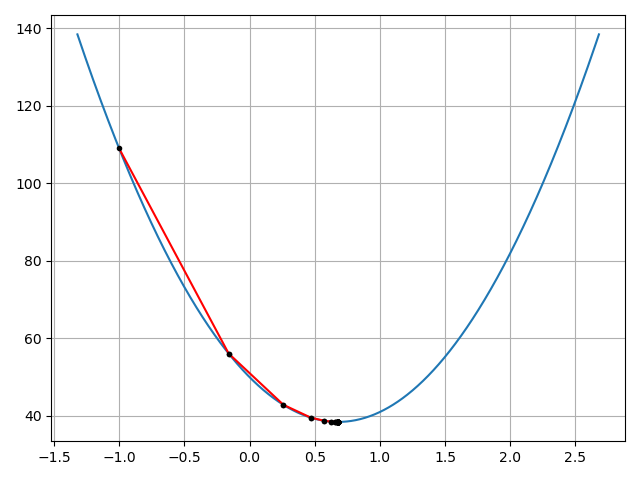
\includegraphics[width=\columnwidth]{11/10/3/14/grad/figs/grad_desc.png}
        \caption{Gradient descent to get the optimal $\lambda$.}
        \label{fig:11/10/3/14/grad/grad-desc}
    \end{figure}

%
\item
Find the maximum and minimum values of  
	\begin{enumerate}
\item Find the minimum value of the function $f\brak{x} = \brak{2x-1}^2 + 3$ using Gradient Descent method. \\ 
\solution 
\label{12/6/5/1/1/2}
\iffalse
\documentclass[12pt]{article}
\usepackage{graphicx}
\usepackage[none]{hyphenat}
\usepackage{graphicx}
\usepackage{listings}
\usepackage[english]{babel}
\usepackage{graphicx}
\usepackage{caption} 
\usepackage{booktabs}
\usepackage{array}
\usepackage{amssymb} % for \because
\usepackage{amsmath}   % for having text in math mode
\usepackage{extarrows} % for Row operations arrows
\usepackage{listings}
\lstset{
  frame=single,
  breaklines=true
}
\usepackage{hyperref}
\usepackage{mathtools}

%Following 2 lines were added to remove the blank page at the beginning
\usepackage{atbegshi}% http://ctan.org/pkg/atbegshi
\AtBeginDocument{\AtBeginShipoutNext{\AtBeginShipoutDiscard}}


%New macro definitions
\newcommand{\mydet}[1]{\ensuremath{\begin{vmatrix}#1\end{vmatrix}}}
\providecommand{\brak}[1]{\ensuremath{\left(#1\right)}}
\providecommand{\sbrak}[1]{\ensuremath{{}\left[#1\right]}}
\providecommand{\norm}[1]{\left\lVert#1\right\rVert}
\providecommand{\abs}[1]{\left\vert#1\right\vert}
\newcommand{\solution}{\noindent \textbf{Solution: }}
\newcommand{\myvec}[1]{\ensuremath{\begin{pmatrix}#1\end{pmatrix}}}
\let\vec\mathbf


\begin{document}

\begin{center}
\title{\textbf{Convex Optimization}}
\date{\vspace{-5ex}} %Not to print date automatically
\maketitle
\end{center}
\setcounter{page}{1}

\section{12$^{th}$ Maths - Chapter 6}
This is Problem-1(i) from Exercise 6.5
\begin{enumerate}
		\fi
The given function has a minimum value as shown in Figure \ref{fig:12/6/5/1/1/2Fig1}.  
\begin{align}
        \label{eq:12/6/5/1/1/2Eq1}
	f^\prime\brak{x} &= 8x-4 
\end{align}
The minimum value of the function is calculated using Gradient Descent method as below 
\begin{align}
	\label{eq:12/6/5/1/1/2grad_des}
	x_{n+1} &= x_n - \alpha \nabla f\brak{x_n}
\end{align}
Choosing
\begin{enumerate}
\item $\alpha$ = 0.001
\item precision = 0.0000001
\item n = 10000000 
\item $x_0$ = -5 
\end{enumerate}
\begin{align}
	x_{min} &= \frac{1}{2}, f\brak{x}_{min} = 3 
\end{align}
\begin{figure}[!h]
	\begin{center}
		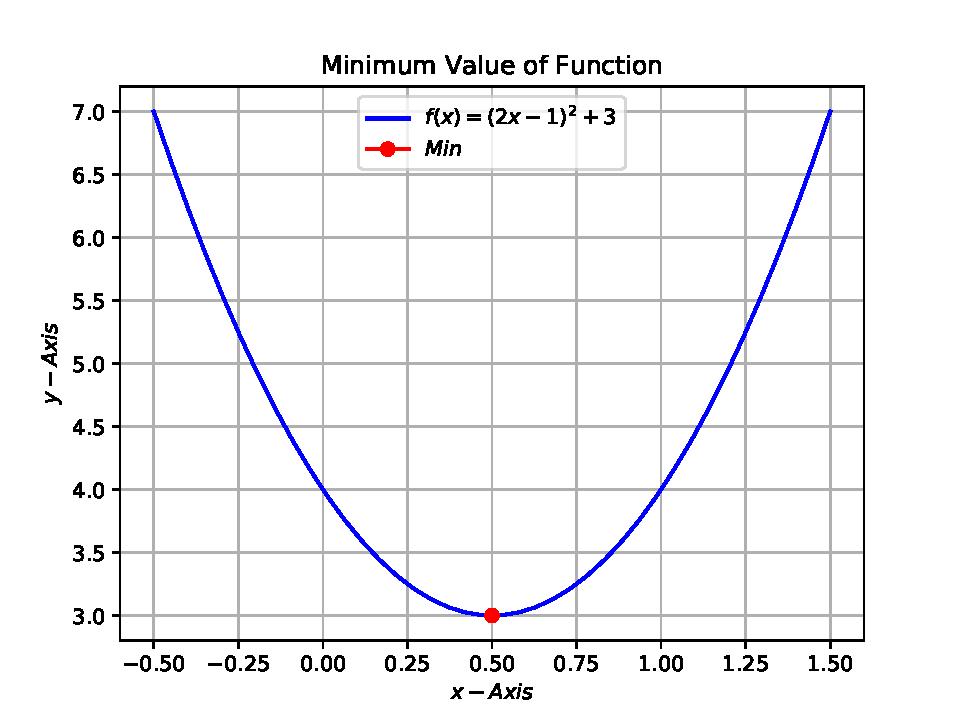
\includegraphics[width=\columnwidth]{12/6/5/1/1/2/figs/Gradient.pdf}
	\end{center}
\caption{}
\label{fig:12/6/5/1/1/2Fig1}
\end{figure}

	\end{enumerate}
 \item The point on the curve 
    \begin{align}
        x^2 = 2y
        \label{eq:12/6/5/27/curve/grad}
    \end{align}
    which is nearest to the point 
    $\vec{P} = \myvec{0\\5}$ is
    \begin{enumerate}
        \item $\myvec{2\sqrt{2}\\4}$
        \item $\myvec{2\sqrt{2}\\0}$
        \item $\myvec{0\\0}$
        \item $\myvec{2\\2}$
    \end{enumerate}
\solution 
\label{12/6/5/27/nonconv/grad}
\iffalse
\documentclass[journal,12pt,twocolumn]{IEEEtran}
\usepackage{setspace}
\usepackage{gensymb}
\usepackage{xcolor}
\usepackage{caption}
\singlespacing
\usepackage{siunitx}
\usepackage[cmex10]{amsmath}
\usepackage{mathtools}
\usepackage{hyperref}
\usepackage{amsthm}
\usepackage{mathrsfs}
\usepackage{txfonts}
\usepackage{stfloats}
\usepackage{cite}
\usepackage{cases}
\usepackage{subfig}
\usepackage{longtable}
\usepackage{multirow}
\usepackage{enumitem}
\usepackage{bm}
\usepackage{mathtools}
\usepackage{listings}
\usepackage{tikz}
\usetikzlibrary{shapes,arrows,positioning}
\usepackage{circuitikz}
\renewcommand{\vec}[1]{\boldsymbol{\mathbf{#1}}}
\DeclareMathOperator*{\Res}{Res}
\renewcommand\thesection{\arabic{section}}
\renewcommand\thesubsection{\thesection.\arabic{subsection}}
\renewcommand\thesubsubsection{\thesubsection.\arabic{subsubsection}}

\renewcommand\thesectiondis{\arabic{section}}
\renewcommand\thesubsectiondis{\thesectiondis.\arabic{subsection}}
\renewcommand\thesubsubsectiondis{\thesubsectiondis.\arabic{subsubsection}}
\hyphenation{op-tical net-works semi-conduc-tor}

\lstset{
language=Python,
frame=single, 
breaklines=true,
columns=fullflexible
}
\begin{document}
\theoremstyle{definition}
\newtheorem{theorem}{Theorem}[section]
\newtheorem{problem}{Problem}
\newtheorem{proposition}{Proposition}[section]
\newtheorem{lemma}{Lemma}[section]
\newtheorem{corollary}[theorem]{Corollary}
\newtheorem{example}{Example}[section]
\newtheorem{definition}{Definition}[section]
\newcommand{\BEQA}{\begin{eqnarray}}
\newcommand{\EEQA}{\end{eqnarray}}
\newcommand{\define}{\stackrel{\triangle}{=}}
\newcommand{\myvec}[1]{\ensuremath{\begin{pmatrix}#1\end{pmatrix}}}
\newcommand{\mydet}[1]{\ensuremath{\begin{vmatrix}#1\end{vmatrix}}}
\bibliographystyle{IEEEtran}
\providecommand{\nCr}[2]{\,^{#1}C_{#2}} % nCr
\providecommand{\nPr}[2]{\,^{#1}P_{#2}} % nPr
\providecommand{\mbf}{\mathbf}
\providecommand{\pr}[1]{\ensuremath{\Pr\left(#1\right)}}
\providecommand{\qfunc}[1]{\ensuremath{Q\left(#1\right)}}
\providecommand{\sbrak}[1]{\ensuremath{{}\left[#1\right]}}
\providecommand{\lsbrak}[1]{\ensuremath{{}\left[#1\right.}}
\providecommand{\rsbrak}[1]{\ensuremath{{}\left.#1\right]}}
\providecommand{\brak}[1]{\ensuremath{\left(#1\right)}}
\providecommand{\lbrak}[1]{\ensuremath{\left(#1\right.}}
\providecommand{\rbrak}[1]{\ensuremath{\left.#1\right)}}
\providecommand{\cbrak}[1]{\ensuremath{\left\{#1\right\}}}
\providecommand{\lcbrak}[1]{\ensuremath{\left\{#1\right.}}
\providecommand{\rcbrak}[1]{\ensuremath{\left.#1\right\}}}
\theoremstyle{remark}
\newtheorem{rem}{Remark}
\newcommand{\sgn}{\mathop{\mathrm{sgn}}}
\newcommand{\rect}{\mathop{\mathrm{rect}}}
\newcommand{\sinc}{\mathop{\mathrm{sinc}}}
\providecommand{\abs}[1]{\left\vert#1\right\vert}
\providecommand{\res}[1]{\Res\displaylimits_{#1}} 
\providecommand{\norm}[1]{\left\Vert#1\right\Vert}
\providecommand{\mtx}[1]{\mathbf{#1}}
\providecommand{\mean}[1]{E\left[ #1 \right]}
\providecommand{\fourier}{\overset{\mathcal{F}}{ \rightleftharpoons}}
\providecommand{\ztrans}{\overset{\mathcal{Z}}{ \rightleftharpoons}}
\providecommand{\system}[1]{\overset{\mathcal{#1}}{ \longleftrightarrow}}
\newcommand{\solution}{\noindent \textbf{Solution: }}
\providecommand{\dec}[2]{\ensuremath{\overset{#1}{\underset{#2}{\gtrless}}}}
\let\StandardTheFigure\thefigure
\def\putbox#1#2#3{\makebox[0in][l]{\makebox[#1][l]{}\raisebox{\baselineskip}[0in][0in]{\raisebox{#2}[0in][0in]{#3}}}}
     \def\rightbox#1{\makebox[0in][r]{#1}}
     \def\centbox#1{\makebox[0in]{#1}}
     \def\topbox#1{\raisebox{-\baselineskip}[0in][0in]{#1}}
     \def\midbox#1{\raisebox{-0.5\baselineskip}[0in][0in]{#1}}

\vspace{3cm}
\title{Quadratic Programming Assignment}
\author{Gautam Singh}
\maketitle
\bigskip

\begin{abstract}
    This document contains the solution to Question 27 of Exercise 5 in Chapter
    6 of the class 12 NCERT textbook.
\end{abstract}

\begin{enumerate}
  
    \solution 
    \fi
		We need to find
    \begin{align}
        \min_{\vec{x}} g\brak{\vec{x}} &= \norm{\vec{x}-\vec{P}}^2 \label{eq:12/6/5/27/nonconv/grad/cost} \\
        \textrm{s.t. } h\brak{\vec{x}} &= \vec{x}^\top\vec{Vx} + 2\vec{u}^\top\vec{x} = 0 \label{eq:12/6/5/27/nonconv/grad/constr}
    \end{align}
    where
    \begin{align}
        \vec{V} = \myvec{1&0\\0&0},\ \vec{u} = \myvec{0\\-1}
    \end{align}
    We find the required minima using constrained gradient descent in 
    Fig. \ref{fig:12/6/5/27/nonconv/grad/gd-pits}, plotted using the Python code 
    \texttt{codes/grad\_pits.py}.
    \begin{figure}[!ht]
        \centering
        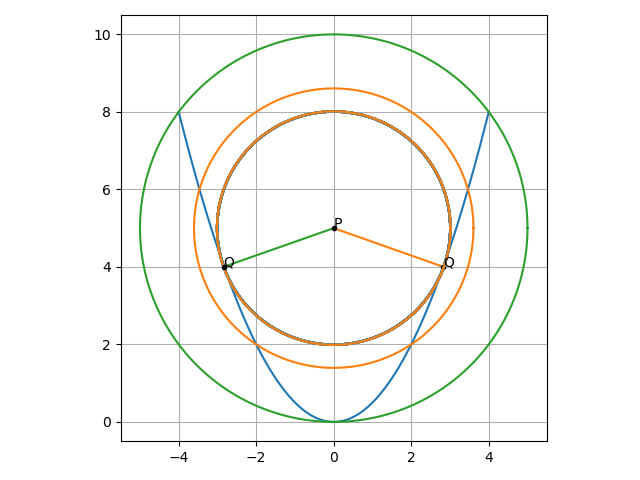
\includegraphics[width=\columnwidth]{12/6/5/27/nonconv/grad/figs/grad_pits.png}
        \caption{Gradient descent for a nonconvex optimization problem.}
        \label{fig:12/6/5/27/nonconv/grad/gd-pits}
    \end{figure}

  \item Find the point on the curve 
    \begin{align}
        x^2 = 2y
        \label{eq:12/6/5/27/conv/gradcurve}
    \end{align}
    which is nearest to the point 
    $\vec{P} = \myvec{2\\1}$.
    \\
\solution 
\label{12/6/5/27/conv/grad}
\iffalse
\documentclass[journal,12pt,twocolumn]{IEEEtran}
\usepackage{setspace}
\usepackage{gensymb}
\usepackage{xcolor}
\usepackage{caption}
\singlespacing
\usepackage{siunitx}
\usepackage[cmex10]{amsmath}
\usepackage{mathtools}
\usepackage{hyperref}
\usepackage{amsthm}
\usepackage{mathrsfs}
\usepackage{txfonts}
\usepackage{stfloats}
\usepackage{cite}
\usepackage{cases}
\usepackage{subfig}
\usepackage{longtable}
\usepackage{multirow}
\usepackage{enumitem}
\usepackage{bm}
\usepackage{mathtools}
\usepackage{listings}
\usepackage{tikz}
\usetikzlibrary{shapes,arrows,positioning}
\usepackage{circuitikz}
\renewcommand{\vec}[1]{\boldsymbol{\mathbf{#1}}}
\DeclareMathOperator*{\Res}{Res}
\renewcommand\thesection{\arabic{section}}
\renewcommand\thesubsection{\thesection.\arabic{subsection}}
\renewcommand\thesubsubsection{\thesubsection.\arabic{subsubsection}}

\renewcommand\thesectiondis{\arabic{section}}
\renewcommand\thesubsectiondis{\thesectiondis.\arabic{subsection}}
\renewcommand\thesubsubsectiondis{\thesubsectiondis.\arabic{subsubsection}}
\hyphenation{op-tical net-works semi-conduc-tor}

\lstset{
language=Python,
frame=single, 
breaklines=true,
columns=fullflexible
}
\begin{document}
\theoremstyle{definition}
\newtheorem{theorem}{Theorem}[section]
\newtheorem{problem}{Problem}
\newtheorem{proposition}{Proposition}[section]
\newtheorem{lemma}{Lemma}[section]
\newtheorem{corollary}[theorem]{Corollary}
\newtheorem{example}{Example}[section]
\newtheorem{definition}{Definition}[section]
\newcommand{\BEQA}{\begin{eqnarray}}
\newcommand{\EEQA}{\end{eqnarray}}
\newcommand{\define}{\stackrel{\triangle}{=}}
\newcommand{\myvec}[1]{\ensuremath{\begin{pmatrix}#1\end{pmatrix}}}
\newcommand{\mydet}[1]{\ensuremath{\begin{vmatrix}#1\end{vmatrix}}}
\bibliographystyle{IEEEtran}
\providecommand{\nCr}[2]{\,^{#1}C_{#2}} % nCr
\providecommand{\nPr}[2]{\,^{#1}P_{#2}} % nPr
\providecommand{\mbf}{\mathbf}
\providecommand{\pr}[1]{\ensuremath{\Pr\left(#1\right)}}
\providecommand{\qfunc}[1]{\ensuremath{Q\left(#1\right)}}
\providecommand{\sbrak}[1]{\ensuremath{{}\left[#1\right]}}
\providecommand{\lsbrak}[1]{\ensuremath{{}\left[#1\right.}}
\providecommand{\rsbrak}[1]{\ensuremath{{}\left.#1\right]}}
\providecommand{\brak}[1]{\ensuremath{\left(#1\right)}}
\providecommand{\lbrak}[1]{\ensuremath{\left(#1\right.}}
\providecommand{\rbrak}[1]{\ensuremath{\left.#1\right)}}
\providecommand{\cbrak}[1]{\ensuremath{\left\{#1\right\}}}
\providecommand{\lcbrak}[1]{\ensuremath{\left\{#1\right.}}
\providecommand{\rcbrak}[1]{\ensuremath{\left.#1\right\}}}
\theoremstyle{remark}
\newtheorem{rem}{Remark}
\newcommand{\sgn}{\mathop{\mathrm{sgn}}}
\newcommand{\rect}{\mathop{\mathrm{rect}}}
\newcommand{\sinc}{\mathop{\mathrm{sinc}}}
\providecommand{\abs}[1]{\left\vert#1\right\vert}
\providecommand{\res}[1]{\Res\displaylimits_{#1}} 
\providecommand{\norm}[1]{\left\Vert#1\right\Vert}
\providecommand{\mtx}[1]{\mathbf{#1}}
\providecommand{\mean}[1]{E\left[ #1 \right]}
\providecommand{\fourier}{\overset{\mathcal{F}}{ \rightleftharpoons}}
\providecommand{\ztrans}{\overset{\mathcal{Z}}{ \rightleftharpoons}}
\providecommand{\system}[1]{\overset{\mathcal{#1}}{ \longleftrightarrow}}
\newcommand{\solution}{\noindent \textbf{Solution: }}
\providecommand{\dec}[2]{\ensuremath{\overset{#1}{\underset{#2}{\gtrless}}}}
\let\StandardTheFigure\thefigure
\def\putbox#1#2#3{\makebox[0in][l]{\makebox[#1][l]{}\raisebox{\baselineskip}[0in][0in]{\raisebox{#2}[0in][0in]{#3}}}}
     \def\rightbox#1{\makebox[0in][r]{#1}}
     \def\centbox#1{\makebox[0in]{#1}}
     \def\topbox#1{\raisebox{-\baselineskip}[0in][0in]{#1}}
     \def\midbox#1{\raisebox{-0.5\baselineskip}[0in][0in]{#1}}

\vspace{3cm}
\title{Quadratic Programming Assignment}
\author{Gautam Singh}
\maketitle
\bigskip

\begin{abstract}
    This document contains the solution to a modification to Question 27 of 
    Exercise 5 in Chapter 6 of the class 12 NCERT textbook.
\end{abstract}

\begin{enumerate}
      \solution 
\fi
		We need to find
    \begin{align}
        \min_{\vec{x}} g\brak{\vec{x}} &= \norm{\vec{x}-\vec{P}}^2 \label{eq:12/6/5/27/conv/gradcost} \\
        \textrm{s.t. } h\brak{\vec{x}} &= \vec{x}^\top\vec{Vx} + 2\vec{u}^\top\vec{x} = 0 \label{eq:12/6/5/27/conv/gradconstr}
    \end{align}
    where
    \begin{align}
        \vec{V} = \myvec{1&0\\0&0},\ \vec{u} = \myvec{0\\-1}
    \end{align}

    We find the required minima using constrained gradient descent in 
    Fig. \ref{fig:12/6/5/27/conv/gradgd-pits}, plotted using Python.
    \begin{figure}[!ht]
        \centering
        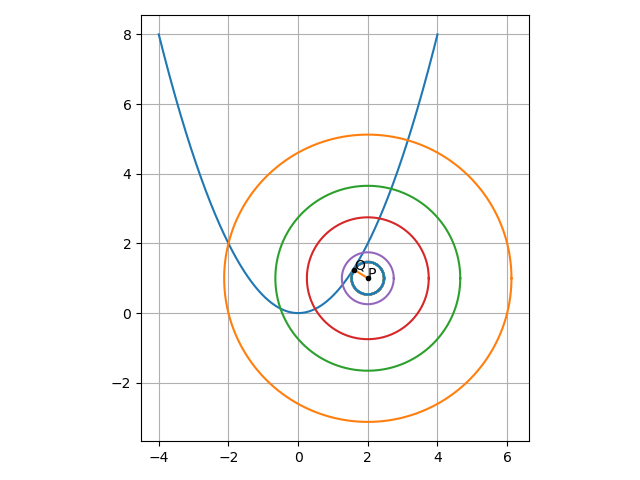
\includegraphics[width=\columnwidth]{12/6/5/27/conv/grad/figs/grad_pits.png}
        \caption{Gradient descent for a convex optimization problem.}
        \label{fig:12/6/5/27/conv/gradgd-pits}
    \end{figure}




\iffalse
\item
\label{12/6/5/2}
%\iffalse
\documentclass[journal,12pt,twocolumn]{IEEEtran}
\usepackage{setspace}
\usepackage{gensymb}
\usepackage{xcolor}
\usepackage{caption}
\singlespacing
\usepackage{siunitx}
\usepackage[cmex10]{amsmath}
\usepackage{mathtools}
\usepackage{hyperref}
\usepackage{amsthm}
\usepackage{mathrsfs}
\usepackage{txfonts}
\usepackage{stfloats}
\usepackage{cite}
\usepackage{cases}
\usepackage{subfig}
\usepackage{longtable}
\usepackage{multirow}
\usepackage{enumitem}
\usepackage{bm}
\usepackage{mathtools}
\usepackage{listings}
\usepackage{tikz}
\usetikzlibrary{shapes,arrows,positioning}
\usepackage{circuitikz}
\renewcommand{\vec}[1]{\boldsymbol{\mathbf{#1}}}
\DeclareMathOperator*{\Res}{Res}
\renewcommand\thesection{\arabic{section}}
\renewcommand\thesubsection{\thesection.\arabic{subsection}}
\renewcommand\thesubsubsection{\thesubsection.\arabic{subsubsection}}

\renewcommand\thesectiondis{\arabic{section}}
\renewcommand\thesubsectiondis{\thesectiondis.\arabic{subsection}}
\renewcommand\thesubsubsectiondis{\thesubsectiondis.\arabic{subsubsection}}
\hyphenation{op-tical net-works semi-conduc-tor}

\lstset{
language=Python,
frame=single, 
breaklines=true,
columns=fullflexible
}
\begin{document}
\theoremstyle{definition}
\newtheorem{theorem}{Theorem}[section]
\newtheorem{problem}{Problem}
\newtheorem{proposition}{Proposition}[section]
\newtheorem{lemma}{Lemma}[section]
\newtheorem{corollary}[theorem]{Corollary}
\newtheorem{example}{Example}[section]
\newtheorem{definition}{Definition}[section]
\newcommand{\BEQA}{\begin{eqnarray}}
\newcommand{\EEQA}{\end{eqnarray}}
\newcommand{\define}{\stackrel{\triangle}{=}}
\newcommand{\myvec}[1]{\ensuremath{\begin{pmatrix}#1\end{pmatrix}}}
\newcommand{\mydet}[1]{\ensuremath{\begin{vmatrix}#1\end{vmatrix}}}
\bibliographystyle{IEEEtran}
\providecommand{\nCr}[2]{\,^{#1}C_{#2}} % nCr
\providecommand{\nPr}[2]{\,^{#1}P_{#2}} % nPr
\providecommand{\mbf}{\mathbf}
\providecommand{\pr}[1]{\ensuremath{\Pr\left(#1\right)}}
\providecommand{\qfunc}[1]{\ensuremath{Q\left(#1\right)}}
\providecommand{\sbrak}[1]{\ensuremath{{}\left[#1\right]}}
\providecommand{\lsbrak}[1]{\ensuremath{{}\left[#1\right.}}
\providecommand{\rsbrak}[1]{\ensuremath{{}\left.#1\right]}}
\providecommand{\brak}[1]{\ensuremath{\left(#1\right)}}
\providecommand{\lbrak}[1]{\ensuremath{\left(#1\right.}}
\providecommand{\rbrak}[1]{\ensuremath{\left.#1\right)}}
\providecommand{\cbrak}[1]{\ensuremath{\left\{#1\right\}}}
\providecommand{\lcbrak}[1]{\ensuremath{\left\{#1\right.}}
\providecommand{\rcbrak}[1]{\ensuremath{\left.#1\right\}}}
\theoremstyle{remark}
\newtheorem{rem}{Remark}
\newcommand{\sgn}{\mathop{\mathrm{sgn}}}
\newcommand{\rect}{\mathop{\mathrm{rect}}}
\newcommand{\sinc}{\mathop{\mathrm{sinc}}}
\providecommand{\abs}[1]{\left\vert#1\right\vert}
\providecommand{\res}[1]{\Res\displaylimits_{#1}} 
\providecommand{\norm}[1]{\left\Vert#1\right\Vert}
\providecommand{\mtx}[1]{\mathbf{#1}}
\providecommand{\mean}[1]{E\left[ #1 \right]}
\providecommand{\fourier}{\overset{\mathcal{F}}{ \rightleftharpoons}}
\providecommand{\ztrans}{\overset{\mathcal{Z}}{ \rightleftharpoons}}
\providecommand{\system}[1]{\overset{\mathcal{#1}}{ \longleftrightarrow}}
\newcommand{\solution}{\noindent \textbf{Solution: }}
\providecommand{\dec}[2]{\ensuremath{\overset{#1}{\underset{#2}{\gtrless}}}}
\let\StandardTheFigure\thefigure
\def\putbox#1#2#3{\makebox[0in][l]{\makebox[#1][l]{}\raisebox{\baselineskip}[0in][0in]{\raisebox{#2}[0in][0in]{#3}}}}
     \def\rightbox#1{\makebox[0in][r]{#1}}
     \def\centbox#1{\makebox[0in]{#1}}
     \def\topbox#1{\raisebox{-\baselineskip}[0in][0in]{#1}}
     \def\midbox#1{\raisebox{-0.5\baselineskip}[0in][0in]{#1}}

\vspace{3cm}
\title{Quadratic Programming Assignment}
\author{Gautam Singh}
\maketitle
\bigskip

\begin{abstract}
    This document contains the solution to a modification to Question 27 of 
    Exercise 5 in Chapter 6 of the class 12 NCERT textbook.
\end{abstract}

\begin{enumerate}
      \solution 
\fi
		We need to find
    \begin{align}
        \min_{\vec{x}} g\brak{\vec{x}} &= \norm{\vec{x}-\vec{P}}^2 \label{eq:12/6/5/27/conv/gradcost} \\
        \textrm{s.t. } h\brak{\vec{x}} &= \vec{x}^\top\vec{Vx} + 2\vec{u}^\top\vec{x} = 0 \label{eq:12/6/5/27/conv/gradconstr}
    \end{align}
    where
    \begin{align}
        \vec{V} = \myvec{1&0\\0&0},\ \vec{u} = \myvec{0\\-1}
    \end{align}

    We find the required minima using constrained gradient descent in 
    Fig. \ref{fig:12/6/5/27/conv/gradgd-pits}, plotted using Python.
    \begin{figure}[!ht]
        \centering
        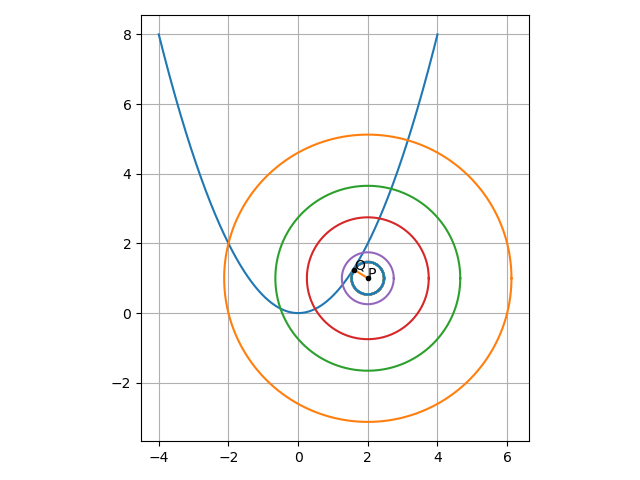
\includegraphics[width=\columnwidth]{12/6/5/27/conv/grad/figs/grad_pits.png}
        \caption{Gradient descent for a convex optimization problem.}
        \label{fig:12/6/5/27/conv/gradgd-pits}
    \end{figure}

\item
\label{12/6/5/3}
\iffalse
\documentclass[journal,12pt,twocolumn]{IEEEtran}
\usepackage{setspace}
\usepackage{gensymb}
\usepackage{xcolor}
\usepackage{caption}
\singlespacing
\usepackage{siunitx}
\usepackage[cmex10]{amsmath}
\usepackage{mathtools}
\usepackage{hyperref}
\usepackage{amsthm}
\usepackage{mathrsfs}
\usepackage{txfonts}
\usepackage{stfloats}
\usepackage{cite}
\usepackage{cases}
\usepackage{subfig}
\usepackage{longtable}
\usepackage{multirow}
\usepackage{enumitem}
\usepackage{bm}
\usepackage{mathtools}
\usepackage{listings}
\usepackage{tikz}
\usetikzlibrary{shapes,arrows,positioning}
\usepackage{circuitikz}
\renewcommand{\vec}[1]{\boldsymbol{\mathbf{#1}}}
\DeclareMathOperator*{\Res}{Res}
\renewcommand\thesection{\arabic{section}}
\renewcommand\thesubsection{\thesection.\arabic{subsection}}
\renewcommand\thesubsubsection{\thesubsection.\arabic{subsubsection}}

\renewcommand\thesectiondis{\arabic{section}}
\renewcommand\thesubsectiondis{\thesectiondis.\arabic{subsection}}
\renewcommand\thesubsubsectiondis{\thesubsectiondis.\arabic{subsubsection}}
\hyphenation{op-tical net-works semi-conduc-tor}

\lstset{
language=Python,
frame=single, 
breaklines=true,
columns=fullflexible
}
\begin{document}
\theoremstyle{definition}
\newtheorem{theorem}{Theorem}[section]
\newtheorem{problem}{Problem}
\newtheorem{proposition}{Proposition}[section]
\newtheorem{lemma}{Lemma}[section]
\newtheorem{corollary}[theorem]{Corollary}
\newtheorem{example}{Example}[section]
\newtheorem{definition}{Definition}[section]
\newcommand{\BEQA}{\begin{eqnarray}}
\newcommand{\EEQA}{\end{eqnarray}}
\newcommand{\define}{\stackrel{\triangle}{=}}
\newcommand{\myvec}[1]{\ensuremath{\begin{pmatrix}#1\end{pmatrix}}}
\newcommand{\mydet}[1]{\ensuremath{\begin{vmatrix}#1\end{vmatrix}}}
\bibliographystyle{IEEEtran}
\providecommand{\nCr}[2]{\,^{#1}C_{#2}} % nCr
\providecommand{\nPr}[2]{\,^{#1}P_{#2}} % nPr
\providecommand{\mbf}{\mathbf}
\providecommand{\pr}[1]{\ensuremath{\Pr\left(#1\right)}}
\providecommand{\qfunc}[1]{\ensuremath{Q\left(#1\right)}}
\providecommand{\sbrak}[1]{\ensuremath{{}\left[#1\right]}}
\providecommand{\lsbrak}[1]{\ensuremath{{}\left[#1\right.}}
\providecommand{\rsbrak}[1]{\ensuremath{{}\left.#1\right]}}
\providecommand{\brak}[1]{\ensuremath{\left(#1\right)}}
\providecommand{\lbrak}[1]{\ensuremath{\left(#1\right.}}
\providecommand{\rbrak}[1]{\ensuremath{\left.#1\right)}}
\providecommand{\cbrak}[1]{\ensuremath{\left\{#1\right\}}}
\providecommand{\lcbrak}[1]{\ensuremath{\left\{#1\right.}}
\providecommand{\rcbrak}[1]{\ensuremath{\left.#1\right\}}}
\theoremstyle{remark}
\newtheorem{rem}{Remark}
\newcommand{\sgn}{\mathop{\mathrm{sgn}}}
\newcommand{\rect}{\mathop{\mathrm{rect}}}
\newcommand{\sinc}{\mathop{\mathrm{sinc}}}
\providecommand{\abs}[1]{\left\vert#1\right\vert}
\providecommand{\res}[1]{\Res\displaylimits_{#1}} 
\providecommand{\norm}[1]{\left\Vert#1\right\Vert}
\providecommand{\mtx}[1]{\mathbf{#1}}
\providecommand{\mean}[1]{E\left[ #1 \right]}
\providecommand{\fourier}{\overset{\mathcal{F}}{ \rightleftharpoons}}
\providecommand{\ztrans}{\overset{\mathcal{Z}}{ \rightleftharpoons}}
\providecommand{\system}[1]{\overset{\mathcal{#1}}{ \longleftrightarrow}}
\newcommand{\solution}{\noindent \textbf{Solution: }}
\providecommand{\dec}[2]{\ensuremath{\overset{#1}{\underset{#2}{\gtrless}}}}
\let\StandardTheFigure\thefigure
\def\putbox#1#2#3{\makebox[0in][l]{\makebox[#1][l]{}\raisebox{\baselineskip}[0in][0in]{\raisebox{#2}[0in][0in]{#3}}}}
     \def\rightbox#1{\makebox[0in][r]{#1}}
     \def\centbox#1{\makebox[0in]{#1}}
     \def\topbox#1{\raisebox{-\baselineskip}[0in][0in]{#1}}
     \def\midbox#1{\raisebox{-0.5\baselineskip}[0in][0in]{#1}}

\vspace{3cm}
\title{Quadratic Programming Assignment}
\author{Gautam Singh}
\maketitle
\bigskip

\begin{abstract}
    This document contains the solution to a modification to Question 27 of 
    Exercise 5 in Chapter 6 of the class 12 NCERT textbook.
\end{abstract}

\begin{enumerate}
      \solution 
\fi
		We need to find
    \begin{align}
        \min_{\vec{x}} g\brak{\vec{x}} &= \norm{\vec{x}-\vec{P}}^2 \label{eq:12/6/5/27/conv/gradcost} \\
        \textrm{s.t. } h\brak{\vec{x}} &= \vec{x}^\top\vec{Vx} + 2\vec{u}^\top\vec{x} = 0 \label{eq:12/6/5/27/conv/gradconstr}
    \end{align}
    where
    \begin{align}
        \vec{V} = \myvec{1&0\\0&0},\ \vec{u} = \myvec{0\\-1}
    \end{align}

    We find the required minima using constrained gradient descent in 
    Fig. \ref{fig:12/6/5/27/conv/gradgd-pits}, plotted using Python.
    \begin{figure}[!ht]
        \centering
        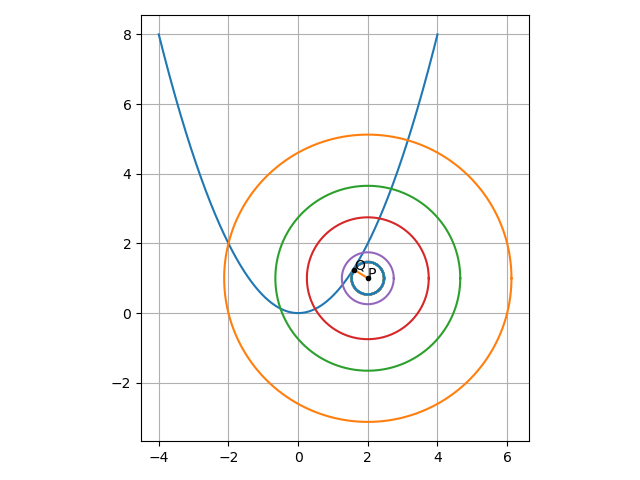
\includegraphics[width=\columnwidth]{12/6/5/27/conv/grad/figs/grad_pits.png}
        \caption{Gradient descent for a convex optimization problem.}
        \label{fig:12/6/5/27/conv/gradgd-pits}
    \end{figure}

\item
\label{12/6/5/4}
\iffalse
\documentclass[journal,12pt,twocolumn]{IEEEtran}
\usepackage{setspace}
\usepackage{gensymb}
\usepackage{xcolor}
\usepackage{caption}
\singlespacing
\usepackage{siunitx}
\usepackage[cmex10]{amsmath}
\usepackage{mathtools}
\usepackage{hyperref}
\usepackage{amsthm}
\usepackage{mathrsfs}
\usepackage{txfonts}
\usepackage{stfloats}
\usepackage{cite}
\usepackage{cases}
\usepackage{subfig}
\usepackage{longtable}
\usepackage{multirow}
\usepackage{enumitem}
\usepackage{bm}
\usepackage{mathtools}
\usepackage{listings}
\usepackage{tikz}
\usetikzlibrary{shapes,arrows,positioning}
\usepackage{circuitikz}
\renewcommand{\vec}[1]{\boldsymbol{\mathbf{#1}}}
\DeclareMathOperator*{\Res}{Res}
\renewcommand\thesection{\arabic{section}}
\renewcommand\thesubsection{\thesection.\arabic{subsection}}
\renewcommand\thesubsubsection{\thesubsection.\arabic{subsubsection}}

\renewcommand\thesectiondis{\arabic{section}}
\renewcommand\thesubsectiondis{\thesectiondis.\arabic{subsection}}
\renewcommand\thesubsubsectiondis{\thesubsectiondis.\arabic{subsubsection}}
\hyphenation{op-tical net-works semi-conduc-tor}

\lstset{
language=Python,
frame=single, 
breaklines=true,
columns=fullflexible
}
\begin{document}
\theoremstyle{definition}
\newtheorem{theorem}{Theorem}[section]
\newtheorem{problem}{Problem}
\newtheorem{proposition}{Proposition}[section]
\newtheorem{lemma}{Lemma}[section]
\newtheorem{corollary}[theorem]{Corollary}
\newtheorem{example}{Example}[section]
\newtheorem{definition}{Definition}[section]
\newcommand{\BEQA}{\begin{eqnarray}}
\newcommand{\EEQA}{\end{eqnarray}}
\newcommand{\define}{\stackrel{\triangle}{=}}
\newcommand{\myvec}[1]{\ensuremath{\begin{pmatrix}#1\end{pmatrix}}}
\newcommand{\mydet}[1]{\ensuremath{\begin{vmatrix}#1\end{vmatrix}}}
\bibliographystyle{IEEEtran}
\providecommand{\nCr}[2]{\,^{#1}C_{#2}} % nCr
\providecommand{\nPr}[2]{\,^{#1}P_{#2}} % nPr
\providecommand{\mbf}{\mathbf}
\providecommand{\pr}[1]{\ensuremath{\Pr\left(#1\right)}}
\providecommand{\qfunc}[1]{\ensuremath{Q\left(#1\right)}}
\providecommand{\sbrak}[1]{\ensuremath{{}\left[#1\right]}}
\providecommand{\lsbrak}[1]{\ensuremath{{}\left[#1\right.}}
\providecommand{\rsbrak}[1]{\ensuremath{{}\left.#1\right]}}
\providecommand{\brak}[1]{\ensuremath{\left(#1\right)}}
\providecommand{\lbrak}[1]{\ensuremath{\left(#1\right.}}
\providecommand{\rbrak}[1]{\ensuremath{\left.#1\right)}}
\providecommand{\cbrak}[1]{\ensuremath{\left\{#1\right\}}}
\providecommand{\lcbrak}[1]{\ensuremath{\left\{#1\right.}}
\providecommand{\rcbrak}[1]{\ensuremath{\left.#1\right\}}}
\theoremstyle{remark}
\newtheorem{rem}{Remark}
\newcommand{\sgn}{\mathop{\mathrm{sgn}}}
\newcommand{\rect}{\mathop{\mathrm{rect}}}
\newcommand{\sinc}{\mathop{\mathrm{sinc}}}
\providecommand{\abs}[1]{\left\vert#1\right\vert}
\providecommand{\res}[1]{\Res\displaylimits_{#1}} 
\providecommand{\norm}[1]{\left\Vert#1\right\Vert}
\providecommand{\mtx}[1]{\mathbf{#1}}
\providecommand{\mean}[1]{E\left[ #1 \right]}
\providecommand{\fourier}{\overset{\mathcal{F}}{ \rightleftharpoons}}
\providecommand{\ztrans}{\overset{\mathcal{Z}}{ \rightleftharpoons}}
\providecommand{\system}[1]{\overset{\mathcal{#1}}{ \longleftrightarrow}}
\newcommand{\solution}{\noindent \textbf{Solution: }}
\providecommand{\dec}[2]{\ensuremath{\overset{#1}{\underset{#2}{\gtrless}}}}
\let\StandardTheFigure\thefigure
\def\putbox#1#2#3{\makebox[0in][l]{\makebox[#1][l]{}\raisebox{\baselineskip}[0in][0in]{\raisebox{#2}[0in][0in]{#3}}}}
     \def\rightbox#1{\makebox[0in][r]{#1}}
     \def\centbox#1{\makebox[0in]{#1}}
     \def\topbox#1{\raisebox{-\baselineskip}[0in][0in]{#1}}
     \def\midbox#1{\raisebox{-0.5\baselineskip}[0in][0in]{#1}}

\vspace{3cm}
\title{Quadratic Programming Assignment}
\author{Gautam Singh}
\maketitle
\bigskip

\begin{abstract}
    This document contains the solution to a modification to Question 27 of 
    Exercise 5 in Chapter 6 of the class 12 NCERT textbook.
\end{abstract}

\begin{enumerate}
      \solution 
\fi
		We need to find
    \begin{align}
        \min_{\vec{x}} g\brak{\vec{x}} &= \norm{\vec{x}-\vec{P}}^2 \label{eq:12/6/5/27/conv/gradcost} \\
        \textrm{s.t. } h\brak{\vec{x}} &= \vec{x}^\top\vec{Vx} + 2\vec{u}^\top\vec{x} = 0 \label{eq:12/6/5/27/conv/gradconstr}
    \end{align}
    where
    \begin{align}
        \vec{V} = \myvec{1&0\\0&0},\ \vec{u} = \myvec{0\\-1}
    \end{align}

    We find the required minima using constrained gradient descent in 
    Fig. \ref{fig:12/6/5/27/conv/gradgd-pits}, plotted using Python.
    \begin{figure}[!ht]
        \centering
        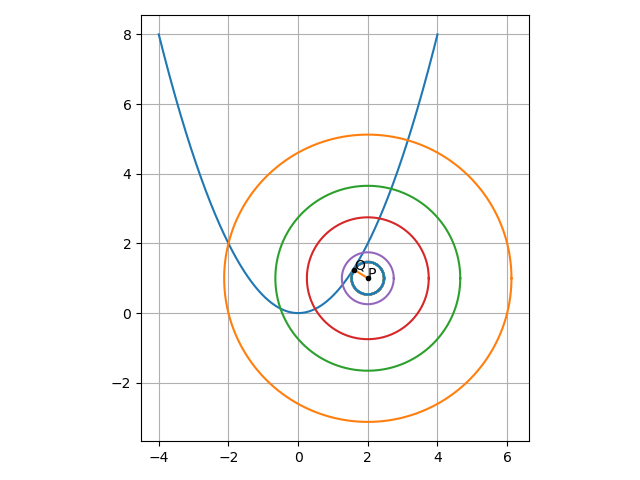
\includegraphics[width=\columnwidth]{12/6/5/27/conv/grad/figs/grad_pits.png}
        \caption{Gradient descent for a convex optimization problem.}
        \label{fig:12/6/5/27/conv/gradgd-pits}
    \end{figure}

\item
\label{12/6/5/5}
\iffalse
\documentclass[journal,12pt,twocolumn]{IEEEtran}
\usepackage{setspace}
\usepackage{gensymb}
\usepackage{xcolor}
\usepackage{caption}
\singlespacing
\usepackage{siunitx}
\usepackage[cmex10]{amsmath}
\usepackage{mathtools}
\usepackage{hyperref}
\usepackage{amsthm}
\usepackage{mathrsfs}
\usepackage{txfonts}
\usepackage{stfloats}
\usepackage{cite}
\usepackage{cases}
\usepackage{subfig}
\usepackage{longtable}
\usepackage{multirow}
\usepackage{enumitem}
\usepackage{bm}
\usepackage{mathtools}
\usepackage{listings}
\usepackage{tikz}
\usetikzlibrary{shapes,arrows,positioning}
\usepackage{circuitikz}
\renewcommand{\vec}[1]{\boldsymbol{\mathbf{#1}}}
\DeclareMathOperator*{\Res}{Res}
\renewcommand\thesection{\arabic{section}}
\renewcommand\thesubsection{\thesection.\arabic{subsection}}
\renewcommand\thesubsubsection{\thesubsection.\arabic{subsubsection}}

\renewcommand\thesectiondis{\arabic{section}}
\renewcommand\thesubsectiondis{\thesectiondis.\arabic{subsection}}
\renewcommand\thesubsubsectiondis{\thesubsectiondis.\arabic{subsubsection}}
\hyphenation{op-tical net-works semi-conduc-tor}

\lstset{
language=Python,
frame=single, 
breaklines=true,
columns=fullflexible
}
\begin{document}
\theoremstyle{definition}
\newtheorem{theorem}{Theorem}[section]
\newtheorem{problem}{Problem}
\newtheorem{proposition}{Proposition}[section]
\newtheorem{lemma}{Lemma}[section]
\newtheorem{corollary}[theorem]{Corollary}
\newtheorem{example}{Example}[section]
\newtheorem{definition}{Definition}[section]
\newcommand{\BEQA}{\begin{eqnarray}}
\newcommand{\EEQA}{\end{eqnarray}}
\newcommand{\define}{\stackrel{\triangle}{=}}
\newcommand{\myvec}[1]{\ensuremath{\begin{pmatrix}#1\end{pmatrix}}}
\newcommand{\mydet}[1]{\ensuremath{\begin{vmatrix}#1\end{vmatrix}}}
\bibliographystyle{IEEEtran}
\providecommand{\nCr}[2]{\,^{#1}C_{#2}} % nCr
\providecommand{\nPr}[2]{\,^{#1}P_{#2}} % nPr
\providecommand{\mbf}{\mathbf}
\providecommand{\pr}[1]{\ensuremath{\Pr\left(#1\right)}}
\providecommand{\qfunc}[1]{\ensuremath{Q\left(#1\right)}}
\providecommand{\sbrak}[1]{\ensuremath{{}\left[#1\right]}}
\providecommand{\lsbrak}[1]{\ensuremath{{}\left[#1\right.}}
\providecommand{\rsbrak}[1]{\ensuremath{{}\left.#1\right]}}
\providecommand{\brak}[1]{\ensuremath{\left(#1\right)}}
\providecommand{\lbrak}[1]{\ensuremath{\left(#1\right.}}
\providecommand{\rbrak}[1]{\ensuremath{\left.#1\right)}}
\providecommand{\cbrak}[1]{\ensuremath{\left\{#1\right\}}}
\providecommand{\lcbrak}[1]{\ensuremath{\left\{#1\right.}}
\providecommand{\rcbrak}[1]{\ensuremath{\left.#1\right\}}}
\theoremstyle{remark}
\newtheorem{rem}{Remark}
\newcommand{\sgn}{\mathop{\mathrm{sgn}}}
\newcommand{\rect}{\mathop{\mathrm{rect}}}
\newcommand{\sinc}{\mathop{\mathrm{sinc}}}
\providecommand{\abs}[1]{\left\vert#1\right\vert}
\providecommand{\res}[1]{\Res\displaylimits_{#1}} 
\providecommand{\norm}[1]{\left\Vert#1\right\Vert}
\providecommand{\mtx}[1]{\mathbf{#1}}
\providecommand{\mean}[1]{E\left[ #1 \right]}
\providecommand{\fourier}{\overset{\mathcal{F}}{ \rightleftharpoons}}
\providecommand{\ztrans}{\overset{\mathcal{Z}}{ \rightleftharpoons}}
\providecommand{\system}[1]{\overset{\mathcal{#1}}{ \longleftrightarrow}}
\newcommand{\solution}{\noindent \textbf{Solution: }}
\providecommand{\dec}[2]{\ensuremath{\overset{#1}{\underset{#2}{\gtrless}}}}
\let\StandardTheFigure\thefigure
\def\putbox#1#2#3{\makebox[0in][l]{\makebox[#1][l]{}\raisebox{\baselineskip}[0in][0in]{\raisebox{#2}[0in][0in]{#3}}}}
     \def\rightbox#1{\makebox[0in][r]{#1}}
     \def\centbox#1{\makebox[0in]{#1}}
     \def\topbox#1{\raisebox{-\baselineskip}[0in][0in]{#1}}
     \def\midbox#1{\raisebox{-0.5\baselineskip}[0in][0in]{#1}}

\vspace{3cm}
\title{Quadratic Programming Assignment}
\author{Gautam Singh}
\maketitle
\bigskip

\begin{abstract}
    This document contains the solution to a modification to Question 27 of 
    Exercise 5 in Chapter 6 of the class 12 NCERT textbook.
\end{abstract}

\begin{enumerate}
      \solution 
\fi
		We need to find
    \begin{align}
        \min_{\vec{x}} g\brak{\vec{x}} &= \norm{\vec{x}-\vec{P}}^2 \label{eq:12/6/5/27/conv/gradcost} \\
        \textrm{s.t. } h\brak{\vec{x}} &= \vec{x}^\top\vec{Vx} + 2\vec{u}^\top\vec{x} = 0 \label{eq:12/6/5/27/conv/gradconstr}
    \end{align}
    where
    \begin{align}
        \vec{V} = \myvec{1&0\\0&0},\ \vec{u} = \myvec{0\\-1}
    \end{align}

    We find the required minima using constrained gradient descent in 
    Fig. \ref{fig:12/6/5/27/conv/gradgd-pits}, plotted using Python.
    \begin{figure}[!ht]
        \centering
        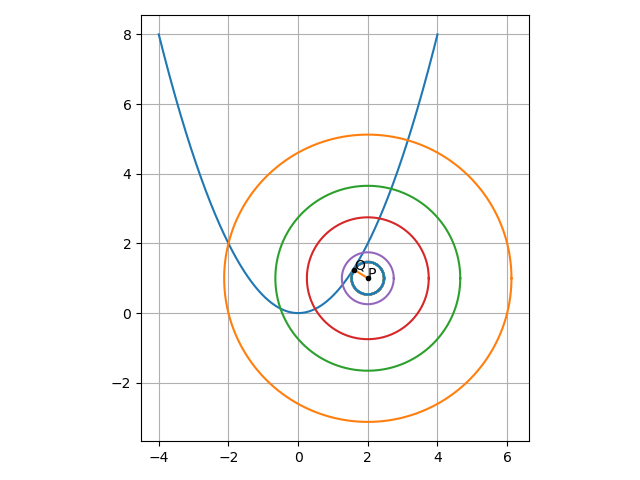
\includegraphics[width=\columnwidth]{12/6/5/27/conv/grad/figs/grad_pits.png}
        \caption{Gradient descent for a convex optimization problem.}
        \label{fig:12/6/5/27/conv/gradgd-pits}
    \end{figure}

\fi
\item
\label{12/6/5/6}
\iffalse
\documentclass[journal,10pt,twocolumn]{article}
\usepackage{graphicx, float}
\usepackage[margin=0.5in]{geometry}
\usepackage{amsmath, bm}
\usepackage{array}
\usepackage{booktabs}
\usepackage[utf8]{inputenc}
\usepackage{amsfonts}
\usepackage{amssymb}
\usepackage{graphicx}
\usepackage{multicol}
\usepackage{tabularx}
\usepackage{hyperref}
\usepackage{mathtools}
\DeclareUnicodeCharacter{2212}{-}
\providecommand{\norm}[1]{\left\lVert#1\right\rVert}
\providecommand{\abs}[1]{\left\vert#1\right\vert}
\let\vec\mathbf
\newcommand{\myvec}[1]{\ensuremath{\begin{pmatrix}#1\end{pmatrix}}}
\newcommand{\mydet}[1]{\ensuremath{\begin{vmatrix}#1\end{vmatrix}}}
\providecommand{\brak}[1]{\ensuremath{\left(#1\right)}}
\providecommand{\lbrak}[1]{\ensuremath{\left(#1\right.}}
\providecommand{\rbrak}[1]{\ensuremath{\left.#1\right)}}
\providecommand{\sbrak}[1]{\ensuremath{{}\left[#1\right]}}
%\providecommand{\norm}[1]{\left\lVert#1\right\rVert}
%\providecommand{\sbrak}[1]{\ensuremath{{}\left[#1\right]}}
%\providecommand{\lsbrak}[1]{\ensuremath{{}\left[#1\right.}}
%\providecommand{\rsbrak}[1]{\ensuremath{{}\left.#1\right]}}
%\providecommand{\brak}[1]{\ensuremath{\left(#1\right)}}
%\providecommand{\lbrak}[1]{\ensuremath{\left(#1\right.}}
%\providecommand{\rbrak}[1]{\ensuremath{\left.#1\right)}}
%\providecommand{\cbrak}[1]{\ensuremath{\left\{#1\right\}}}
%\providecommand{\lcbrak}[1]{\ensuremath{\left\{#1\right.}}
%\providecommand{\rcbrak}[1]{\ensuremath{\left.#1\right\}}}
%\newcommand{\myvec}[1]{\ensuremath{\begin{pmatrix}#1\end{pmatrix}}}
%\let\vec\mathbf

\title{\textbf{Optimization-Basic Assignment}}
\author{Namrath Pinnamaneni \hspace{9cm} FWC22042}
\date{September 2022}

\begin{document}

\maketitle
\paragraph{\textit{Problem Statement} -
\fi
Find the maximum profit that a company can make if the profit function is given by  
\begin{align}
f(x) = 41-72x+18x^2
\end{align}
\\
\solution
\iffalse
A function f(x) is said to be convex if following inequality is true for $\lambda \in [0,1] :$  \label{opt/2/1/a/lemma1}
\begin{align}
    \lambda f(x_1) + (1-\lambda)f(x_2) \geq f(\lambda x_1 + (1-\lambda)x_2)
    \label{eq:12/6/5/62}
\end{align}
\fi
Considering
\begin{align}
    &\lambda\brak{41-72x_1-18x_1^2} + (1-\lambda)\brak{41-72x_2-18x_2^2} \geq \\
    &41-72\brak{\lambda x_1 + (1-\lambda)x_2} - 18\brak{\lambda x_1 + (1-\lambda)x_2}^2,
\end{align}
we obtain
\begin{align}
        18x_1^2\brak{{\lambda^2-\lambda}}+18x_2^2\brak{{\lambda^2-\lambda}}+36x_1x_2\brak{{\lambda^2-\lambda}} &\geq 0 \\
        x_1^2\brak{{\lambda^2-\lambda}}+x_2^2\brak{{\lambda^2-\lambda}}+2x_1x_2\brak{{\lambda^2-\lambda}} &\geq 0 \\
        -\lambda\brak{1-\lambda}\brak{x_1-x_2}^2 &\geq 0 \\
        \implies \lambda\brak{1-\lambda}\brak{x_1-x_2}^2 &\leq 0 \label{eq:12/6/5/67}
\end{align}
which is 
 false for all $\lambda\in(0,1)$. Hence the given function $f(x)$ is concave.
 \iffalse
 For a general quadratic equation
\begin{align}
    f(x)=ax^2+bx+c
\end{align}
\fi
    Using the gradient ascent method,
\begin{align}
    x_n=x_{n-1}+\mu\frac{df(x)}{dx} \label{eq:12/6/5/69}
    \end{align}
    Since
    \begin{align}
    \frac{df(x)}{dx}=-72-36x, \label{eq:12/6/5/610}
\end{align}
substituting \eqref{eq:12/6/5/610} in \eqref{eq:12/6/5/69}, 
\begin{align}
    x_n=x_{n-1}+\mu(-72-36x_{n-1})\label{eq:12/6/5/611}
\end{align}
Choosing
\begin{align}
	x_0 &= 1, \alpha = 0.001,  precision = 0.00000001, 
\\
	f_{max}  &\approx 113,
	x_{max}  \approx -2.0,
\end{align}
which is verified in Fig. 
		\ref{fig:12/6/5/6}.
	\begin{figure}[!ht]
		\centering
		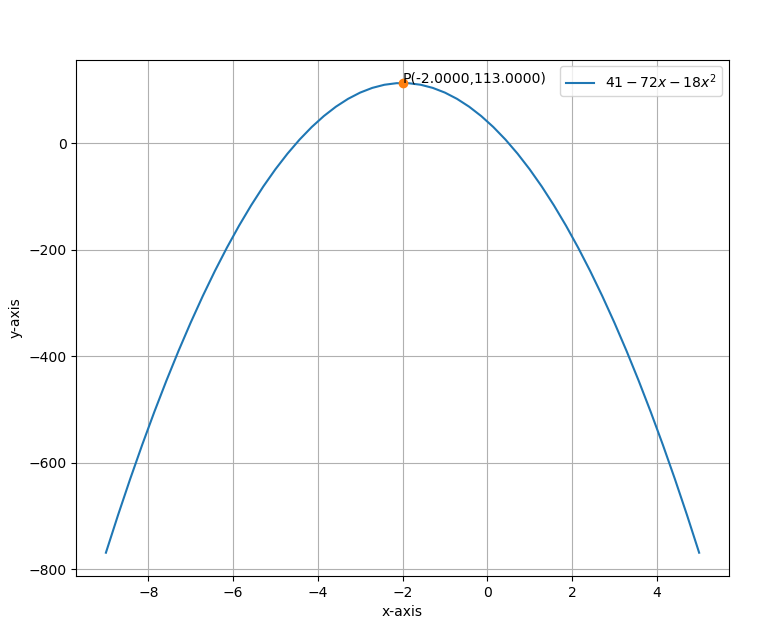
\includegraphics[width=\columnwidth]{12/6/5/6/figs/opt_basic.png}
		\caption{}
		\label{fig:12/6/5/6}
  	\end{figure}
\iffalse
\includegraphics[width=1\columnwidth]{opt_basic.png}
\centering \text{Graph of f(x) = $41-72x+18x^2$}

\end{document}
\fi

\item
\label{12/6/5/7}
\iffalse
\documentclass[journal,10pt,twocolumn]{article}
\usepackage{graphicx, float}
\usepackage[margin=0.5in]{geometry}
\usepackage{amsmath, bm}
\usepackage{array}
\usepackage{booktabs}

\providecommand{\norm}[1]{\left\lVert#1\right\rVert}
\let\vec\mathbf
\newcommand{\myvec}[1]{\ensuremath{\begin{pmatrix}#1\end{pmatrix}}}
\newcommand{\mydet}[1]{\ensuremath{\begin{vmatrix}#1\end{vmatrix}}}

\title{\textbf{Optimization Assignment}}
\author{Pallavarapu Sravan kumar}
\date{October 2022}

\begin{document}

\maketitle
\paragraph{\textit{\large Problem Statement} -
\fi
Find both the maximum value and the minimum value of 
\begin{align}
    f(x) &= 3x^4-8x^3+12x^2-48x+25=0 &  x \in (0,3)
\end{align}
\solution
	\begin{figure}[!ht]
		\centering
		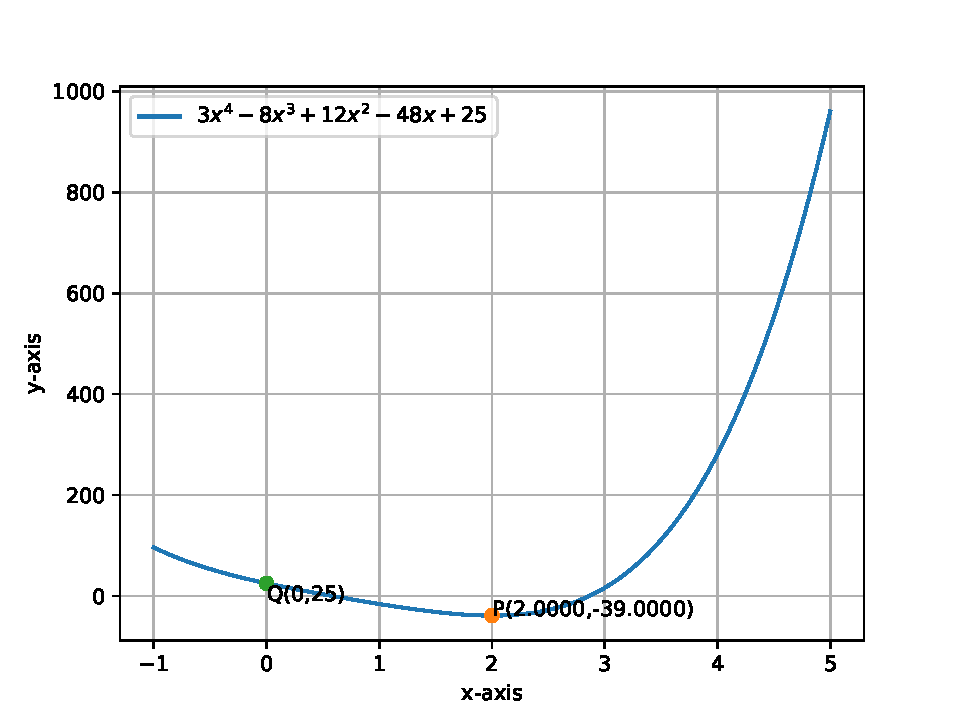
\includegraphics[width=\columnwidth]{12/6/5/7/figs/opt2.pdf}
		\caption{}
		\label{fig:12/6/5/7}
  	\end{figure}
	\iffalse
\section*{\large Figure:}
\begin{figure}[H]
\centering
\includegraphics[width=1\columnwidth]{opt2.pdf}
\caption{Graph of f(x)}
\end{figure}



\section*{Solution:}

Given:
\begin{align}
    f(x) &= 3x^4-8x^3+12x^2-48x+25=0 &  x \in (0,3)
\end{align}
\fi
\begin{align}
    \frac{df(x)}{dx} &= 12x^3-24x^2+24x-48
\end{align}
		The minimum can be found using
\begin{align}
        x_{n+1} &= x_n - \alpha \frac{df(x)}{dx}
	\\
          &= x_n - \alpha (12x_n^3-24x_n^2+24x_n-48)
\end{align}
where 
\begin{enumerate}
\item $\alpha$ = 0.001
\item $x_{n+1}$ is current value
\item $x_{n}$ is previous value
\item precession = 0.00000001
\item maximum iterations = 100000000
\end{enumerate}
as
\begin{align}
 	f_{min}= -39\\
 	x_{min}= 2
    \end{align}
    \iffalse
    \item
For maximum, the 
 Critical point is given by
    \begin{align}
       \frac{df(x)}{dx} &= 0 \\
        \implies x &= 2
    \end{align}
    
    and,end points are $x=0$ and $x=3$ .Using table1
    \begin{table}[htbp]
 \begin{center}
    \begin{tabular}{|l|c|c|c|c|c|c} \hline \textbf{x}
  & \textbf{f(x)} \\
 \hline
0 &25\\ \hline
2&-39 \\ \hline
3 &16  \\ \hline	
\end{tabular}   
\end{center}
\caption{Value of f(x)}
\end{table}

 \begin{align}
        \boxed{\text{Maxima} = 25}\\
        \boxed{\text{Maxima Point} = 0}
    \end{align}
   
\end{document}
\fi

\item
\label{12/6/5/8}
\iffalse
\documentclass[journal,10pt,twocolumn]{article}
\usepackage{graphicx, float}
\usepackage[margin=0.5in]{geometry}
\usepackage{amsmath, bm}
\usepackage{array}
\usepackage{booktabs}
\usepackage{mathtools}

\providecommand{\norm}[1]{\left\lVert#1\right\rVert}
\let\vec\mathbf
\newcommand{\myvec}[1]{\ensuremath{\begin{pmatrix}#1\end{pmatrix}}}
\newcommand{\mydet}[1]{\ensuremath{\begin{vmatrix}#1\end{vmatrix}}}

\title{\textbf{Optimization Assignment}}
\author{Maddu Dinesh}
\date{September 2022}

\begin{document}

\maketitle
\paragraph{\textit{Problem Statement} -
\fi
At what points in the interval (0,2$\pi$) does the function $\sin2x$ attain its maximum value.
\\
\solution
	\begin{figure}[!ht]
		\centering
		\includegraphics[width=\columnwidth]{12/6/5/8/figs/a.png}
		\caption{}
		\label{fig:12/6/5/8}
  	\end{figure}
\iffalse
\section*{\large Figure}

\begin{figure}[H]
\centering
\includegraphics[width=1\columnwidth]{a.png}
\caption{Graph of f(x)}
\label{fig:triangle}
\end{figure}
\section*{\large Solution}

	
    \subsection*{\normalsize Gradient descent}
\fi    
  Since  
    \begin{align}
	\label{eq:12/6/5/8vol_varx}
	    f(x) &= \sin2x,
	    \\
	    f'(x) &= 2\cos2x
	\end{align}
\iffalse
we have to attain the maximum value of sin2x in the interval [0,2$\pi$]. This can be seen in Figure f(x).
\fi
Using gradient ascent, 
\begin{align}
	x_{n+1} &= x_n + \alpha \nabla f(x_n) \\
&=x_n+\alpha(2\cos2x)
\end{align}
Choosing
\begin{align}
	x_0&=0.5,\alpha=0.001, precision = 0.00000001, 
	\\
	f_{max} &= 1.0000,
 	x_{max}= 0.7854.
    \end{align}
   
    

    





 







\iffalse
\item
\label{12/6/5/9}
%\iffalse
\documentclass[journal,12pt,twocolumn]{IEEEtran}
\usepackage{setspace}
\usepackage{gensymb}
\usepackage{xcolor}
\usepackage{caption}
\singlespacing
\usepackage{siunitx}
\usepackage[cmex10]{amsmath}
\usepackage{mathtools}
\usepackage{hyperref}
\usepackage{amsthm}
\usepackage{mathrsfs}
\usepackage{txfonts}
\usepackage{stfloats}
\usepackage{cite}
\usepackage{cases}
\usepackage{subfig}
\usepackage{longtable}
\usepackage{multirow}
\usepackage{enumitem}
\usepackage{bm}
\usepackage{mathtools}
\usepackage{listings}
\usepackage{tikz}
\usetikzlibrary{shapes,arrows,positioning}
\usepackage{circuitikz}
\renewcommand{\vec}[1]{\boldsymbol{\mathbf{#1}}}
\DeclareMathOperator*{\Res}{Res}
\renewcommand\thesection{\arabic{section}}
\renewcommand\thesubsection{\thesection.\arabic{subsection}}
\renewcommand\thesubsubsection{\thesubsection.\arabic{subsubsection}}

\renewcommand\thesectiondis{\arabic{section}}
\renewcommand\thesubsectiondis{\thesectiondis.\arabic{subsection}}
\renewcommand\thesubsubsectiondis{\thesubsectiondis.\arabic{subsubsection}}
\hyphenation{op-tical net-works semi-conduc-tor}

\lstset{
language=Python,
frame=single, 
breaklines=true,
columns=fullflexible
}
\begin{document}
\theoremstyle{definition}
\newtheorem{theorem}{Theorem}[section]
\newtheorem{problem}{Problem}
\newtheorem{proposition}{Proposition}[section]
\newtheorem{lemma}{Lemma}[section]
\newtheorem{corollary}[theorem]{Corollary}
\newtheorem{example}{Example}[section]
\newtheorem{definition}{Definition}[section]
\newcommand{\BEQA}{\begin{eqnarray}}
\newcommand{\EEQA}{\end{eqnarray}}
\newcommand{\define}{\stackrel{\triangle}{=}}
\newcommand{\myvec}[1]{\ensuremath{\begin{pmatrix}#1\end{pmatrix}}}
\newcommand{\mydet}[1]{\ensuremath{\begin{vmatrix}#1\end{vmatrix}}}
\bibliographystyle{IEEEtran}
\providecommand{\nCr}[2]{\,^{#1}C_{#2}} % nCr
\providecommand{\nPr}[2]{\,^{#1}P_{#2}} % nPr
\providecommand{\mbf}{\mathbf}
\providecommand{\pr}[1]{\ensuremath{\Pr\left(#1\right)}}
\providecommand{\qfunc}[1]{\ensuremath{Q\left(#1\right)}}
\providecommand{\sbrak}[1]{\ensuremath{{}\left[#1\right]}}
\providecommand{\lsbrak}[1]{\ensuremath{{}\left[#1\right.}}
\providecommand{\rsbrak}[1]{\ensuremath{{}\left.#1\right]}}
\providecommand{\brak}[1]{\ensuremath{\left(#1\right)}}
\providecommand{\lbrak}[1]{\ensuremath{\left(#1\right.}}
\providecommand{\rbrak}[1]{\ensuremath{\left.#1\right)}}
\providecommand{\cbrak}[1]{\ensuremath{\left\{#1\right\}}}
\providecommand{\lcbrak}[1]{\ensuremath{\left\{#1\right.}}
\providecommand{\rcbrak}[1]{\ensuremath{\left.#1\right\}}}
\theoremstyle{remark}
\newtheorem{rem}{Remark}
\newcommand{\sgn}{\mathop{\mathrm{sgn}}}
\newcommand{\rect}{\mathop{\mathrm{rect}}}
\newcommand{\sinc}{\mathop{\mathrm{sinc}}}
\providecommand{\abs}[1]{\left\vert#1\right\vert}
\providecommand{\res}[1]{\Res\displaylimits_{#1}} 
\providecommand{\norm}[1]{\left\Vert#1\right\Vert}
\providecommand{\mtx}[1]{\mathbf{#1}}
\providecommand{\mean}[1]{E\left[ #1 \right]}
\providecommand{\fourier}{\overset{\mathcal{F}}{ \rightleftharpoons}}
\providecommand{\ztrans}{\overset{\mathcal{Z}}{ \rightleftharpoons}}
\providecommand{\system}[1]{\overset{\mathcal{#1}}{ \longleftrightarrow}}
\newcommand{\solution}{\noindent \textbf{Solution: }}
\providecommand{\dec}[2]{\ensuremath{\overset{#1}{\underset{#2}{\gtrless}}}}
\let\StandardTheFigure\thefigure
\def\putbox#1#2#3{\makebox[0in][l]{\makebox[#1][l]{}\raisebox{\baselineskip}[0in][0in]{\raisebox{#2}[0in][0in]{#3}}}}
     \def\rightbox#1{\makebox[0in][r]{#1}}
     \def\centbox#1{\makebox[0in]{#1}}
     \def\topbox#1{\raisebox{-\baselineskip}[0in][0in]{#1}}
     \def\midbox#1{\raisebox{-0.5\baselineskip}[0in][0in]{#1}}

\vspace{3cm}
\title{Quadratic Programming Assignment}
\author{Gautam Singh}
\maketitle
\bigskip

\begin{abstract}
    This document contains the solution to a modification to Question 27 of 
    Exercise 5 in Chapter 6 of the class 12 NCERT textbook.
\end{abstract}

\begin{enumerate}
      \solution 
\fi
		We need to find
    \begin{align}
        \min_{\vec{x}} g\brak{\vec{x}} &= \norm{\vec{x}-\vec{P}}^2 \label{eq:12/6/5/27/conv/gradcost} \\
        \textrm{s.t. } h\brak{\vec{x}} &= \vec{x}^\top\vec{Vx} + 2\vec{u}^\top\vec{x} = 0 \label{eq:12/6/5/27/conv/gradconstr}
    \end{align}
    where
    \begin{align}
        \vec{V} = \myvec{1&0\\0&0},\ \vec{u} = \myvec{0\\-1}
    \end{align}

    We find the required minima using constrained gradient descent in 
    Fig. \ref{fig:12/6/5/27/conv/gradgd-pits}, plotted using Python.
    \begin{figure}[!ht]
        \centering
        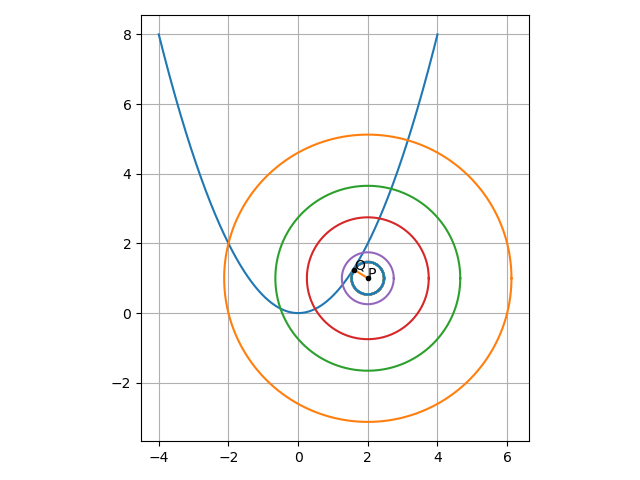
\includegraphics[width=\columnwidth]{12/6/5/27/conv/grad/figs/grad_pits.png}
        \caption{Gradient descent for a convex optimization problem.}
        \label{fig:12/6/5/27/conv/gradgd-pits}
    \end{figure}

\fi
\item
\label{12/6/5/10}
\iffalse
\documentclass[journal,10pt,twocolumn]{article}
\usepackage{graphicx, float}
\usepackage[margin=0.5in]{geometry}
\usepackage{amsmath, bm}
\usepackage{array}
\usepackage{booktabs}
\usepackage[utf8]{inputenc}
\usepackage{amsfonts}
\usepackage{amssymb}
\usepackage{graphicx}
\usepackage{multicol}
\usepackage{tabularx}
\usepackage{hyperref}
\usepackage{mathtools}
\DeclareUnicodeCharacter{2212}{-}
\providecommand{\norm}[1]{\left\lVert#1\right\rVert}
\providecommand{\abs}[1]{\left\vert#1\right\vert}
\let\vec\mathbf
\newcommand{\myvec}[1]{\ensuremath{\begin{pmatrix}#1\end{pmatrix}}}
\newcommand{\mydet}[1]{\ensuremath{\begin{vmatrix}#1\end{vmatrix}}}
\providecommand{\brak}[1]{\ensuremath{\left(#1\right)}}
\providecommand{\lbrak}[1]{\ensuremath{\left(#1\right.}}
\providecommand{\rbrak}[1]{\ensuremath{\left.#1\right)}}
\providecommand{\sbrak}[1]{\ensuremath{{}\left[#1\right]}}
%\providecommand{\norm}[1]{\left\lVert#1\right\rVert}
%\providecommand{\sbrak}[1]{\ensuremath{{}\left[#1\right]}}
%\providecommand{\lsbrak}[1]{\ensuremath{{}\left[#1\right.}}
%\providecommand{\rsbrak}[1]{\ensuremath{{}\left.#1\right]}}
%\providecommand{\brak}[1]{\ensuremath{\left(#1\right)}}
%\providecommand{\lbrak}[1]{\ensuremath{\left(#1\right.}}
%\providecommand{\rbrak}[1]{\ensuremath{\left.#1\right)}}
%\providecommand{\cbrak}[1]{\ensuremath{\left\{#1\right\}}}
%\providecommand{\lcbrak}[1]{\ensuremath{\left\{#1\right.}}
%\providecommand{\rcbrak}[1]{\ensuremath{\left.#1\right\}}}
%\newcommand{\myvec}[1]{\ensuremath{\begin{pmatrix}#1\end{pmatrix}}}
%\let\vec\mathbf

\title{\textbf{Optimization-Basic Assignment}}
\author{V.Meghana \hspace{9cm} FWC22045}
\date{October 2022}

\begin{document}

\maketitle
\paragraph{\textit{Problem Statement} -
\fi
Find the maximum value of $2x^3 – 24x + 107$ in the interval [1, 3]. Find the maximum value of the same function in [–3, –1].
\\
\solution
\iffalse
\section*{\large Solution}
\fi
    Using gradient ascent method,
\begin{align}
    x_n=x_{n-1}+\mu\frac{df(x)}{dx} \label{eq:12/6/5/109}
    \end{align}
    where
    \begin{align}
    \frac{df(x)}{dx}=6x^2-24 \label{eq:12/6/5/1010}
\end{align}
yielding
\begin{align}
    x_n=x_{n-1}+\mu(6x^2-24_{n-1})\label{eq:12/6/5/1011}
\end{align}
Choosing
\begin{align}
	x_0 &= 1, \mu = 0.001 \text{ and precision} = 0.00000001, 
	\\
	f_{max} &  \approx 139,
x_{max}   \approx -2.0
\end{align}
	\begin{figure}[!ht]
		\centering
		\includegraphics[width=\columnwidth]{12/6/5/10/figs/opt_basic.png}
		\caption{}
		\label{fig:12/6/5/10}
  	\end{figure}
\iffalse
\begin{align}
\end{align}
\end{enumerate}

\includegraphics[width=1\columnwidth]{opt_basic.png}
\centering \text{Graph of f(x) = $2x^3-24x+107$}

\end{document}
\fi

\item
\label{12/6/5/11}
\iffalse
\documentclass[10pt,twocolumn]{article}
\usepackage{graphicx}
\usepackage[margin=0.5in]{geometry}
\usepackage[cmex10]{amsmath}
\usepackage{array}
\usepackage{booktabs}
\usepackage{mathtools}
\title{\textbf{Optimization}}
\author{Vemulapalli Bavya Sri}
\date{October 2022}


\providecommand{\norm}[1]{\lVert#1\rVert}
\providecommand{\abs}[1]{\vert#1\vert}
\let\vec\mathbf
\newcommand{\myvec}[1]{\ensuremath{\begin{pmatrix}#1\end{pmatrix}}}
\newcommand{\mydet}[1]{\ensuremath{\begin{vmatrix}#1\end{vmatrix}}}
\providecommand{\brak}[1]{\ensuremath{\left(#1\right)}}
\providecommand{\lbrak}[1]{\ensuremath{\left(#1\right.}}
\providecommand{\rbrak}[1]{\ensuremath{\left.#1\right)}}
\providecommand{\sbrak}[1]{\ensuremath{{}\left[#1\right]}}

\begin{document}

\maketitle
\paragraph{\textit{Problem Statement} -
\fi
It is given that at x=1, the function
$x^4-62x^2+ax+9$ attains its maximum value, on the interval [0,2]. Find the value of a. 
\\
\solution
\iffalse
\section{Solution}
\begin{flushleft}
Given function is,\\
\end{flushleft}
\begin{align}
\label{eqn:1}
    f(x)=x^4-62x^2+ax+9
\end{align}
\subsection{Calculation of Maxima using normal differentiation}
\begin{flushleft}
	\fi
Differentiating the given function,
\begin{align}
\nabla f(x) = 4x^3-124x+a
\end{align}
Since $f$ attains its maximum value on the interval [0,2] at $x=1$,
\begin{align}
\nabla f(1) =0
\implies a=120
\end{align}
\iffalse
\begin{flushleft}
\subsection{Calculation of Maxima using gradient ascent algorithm}
\end{flushleft}
\begin{flushleft}
Maxima of the above equation (1), can be calculated from the following expression,\\
To find,
\end{flushleft}
\begin{align}
\max_{x} f(x)
\end{align}  
\fi
Using gradient descent,
    \begin{align}
	    x_{n+1}&= x_n + \alpha \nabla f(x_n)
	    \\
	    &= x_n + \alpha \brak{4x_n^3-124x_n+120}
    \end{align}
    and choosing
\begin{align}
	x_0&=0.5,\alpha=0.001 \text{ and precision} = 0.00000001, 
	\\
	f_{max} &= 68,
        x_{max} = 1
\end{align}
	\begin{figure}[!ht]
		\centering
		\includegraphics[width=\columnwidth]{12/6/5/11/figs/b.png}
		\caption{}
		\label{fig:12/6/5/11}
  	\end{figure}
\iffalse
\end{flushleft} 
\center

\begin{flushleft}
\section{Construction}
\end{flushleft}

\begin{flushleft}
1. At first, the given function has been differentiated and it is solved by setting f'(x) equal to zero. By using x values, f(x) values are calculated.\\
\vspace{0.25cm}
2. Later, the given function f(x) is solved by gradient ascent algorithm to find maxima and the point at which f(x) is maximum.\\
\vspace{0.25cm}
3. Maxima and related points are, \\
\vspace{0.25cm}
\center
Maxima point, Max=(1 , 68) 
\end{flushleft}

\begin{figure}[h]
\includegraphics[scale=0.6]{b.png}
\caption{Graph}
\label{fig:Graph}
\end{figure}

\end{document}
\fi

\item
\label{12/6/6/14}
\iffalse
\documentclass[10pt,twocolumn]{article}
\usepackage{graphicx}
\usepackage[margin=0.5in]{geometry}
\usepackage[cmex10]{amsmath}
\usepackage{array}
\usepackage{booktabs}
\usepackage{mathtools}
\title{\textbf{Optimization Assignment}}
\author{Sinkona Chinthamalla}

\providecommand{\norm}[1]{\lVert#1\rVert}
\providecommand{\abs}[1]{\vert#1\vert}
\let\vec\mathbf
\newcommand{\myvec}[1]{\ensuremath{\begin{pmatrix}#1\end{pmatrix}}}
\newcommand{\mydet}[1]{\ensuremath{\begin{vmatrix}#1\end{vmatrix}}}
\providecommand{\brak}[1]{\ensuremath{\left(#1\right)}}
\providecommand{\lbrak}[1]{\ensuremath{\left(#1\right.}}
\providecommand{\rbrak}[1]{\ensuremath{\left.#1\right)}}
\providecommand{\sbrak}[1]{\ensuremath{{}\left[#1\right]}}

\begin{document}

\maketitle
\paragraph{\textit{Problem Statement} -
\fi
Find the absolute maximum and minimum values of the function $f$ given by 
\begin{align}
	f(x) = \cos^2x + \sin x,\quad x \in \sbrak{0,\pi} 
\end{align} 
\solution
	\begin{figure}[!ht]
		\centering
		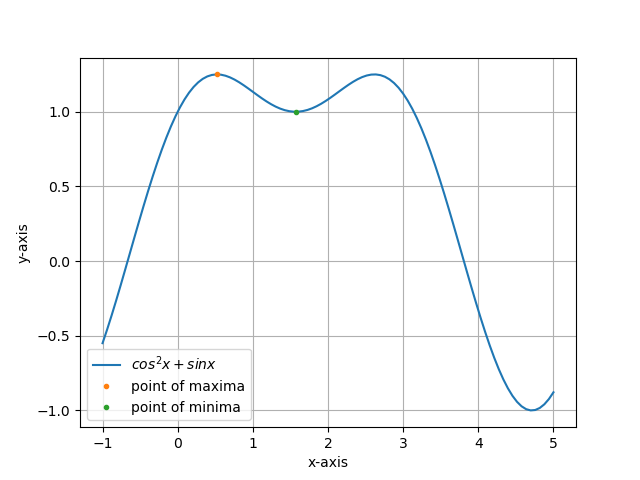
\includegraphics[width=\columnwidth]{12/6/6/14/figs/opt.png}
		\caption{}
		\label{fig:12/6/6/14}
  	\end{figure}
\iffalse

\section{Solution}
\begin{flushleft}
Given function is,\\
\end{flushleft}
\begin{equation}
    f(x)=\cos^2x + \sin x
\end{equation}
\subsection{Calculation using normal differentiation}
\begin{flushleft}
Differentiating (1) yields,
\end{flushleft}
\fi
The derivative of the given function is
\begin{align}
\nabla f(x) = \cos x-2\sin x \cos x 
\end{align}
\iffalse

\noindent Calculating the critical points:
$ \nabla f(x) = 0 $

\begin{equation}
\implies \cos{x} = 0 
\end{equation}
\begin{equation}
\implies -2\sin{x} + 1 = 0
\end{equation}
Therefore, the critical points are 

\begin{equation}
\frac{\pi}{6},\quad\frac{5\pi}{6},\quad\frac{\pi}{2}
\end{equation}

\textbf{1.1.1 Finding absolute maximum and minimum} 
Since given interval is $x \in [0,\pi]$ 

\begin{table}[h]
\centering
\large
\begin{tabular}{|l|l|}
\hline
\textbf{value of x} & \textbf{value of} \\ \hline
At x =0             & 1                 \\ \hline
At x =$ \frac{\pi}{6}$            & $\frac{5}{4}$            \\ \hline
At x =  $ \frac{\pi}{2}$            & 1                 \\ \hline
At x =  $ \frac{5\pi}{6}$            & $\frac{5}{4}$             \\ \hline
at x =       $\pi$       & 1                 \\ \hline
\end{tabular}
\end{table}

Hence, 
\begin{align}
\text{absolute maximum} & =  \frac{5}{4}\\
\text{absolute minimum} & = 1
\end{align}

\subsection{Calculation of Maxima using gradient ascent algorithm}
\fi
The 
maxima is calculated by
\begin{align}
x_{n+1} = x_n + \alpha \nabla f(x_n) 
\\
 &= x_n + \alpha \brak{cosx_n-2sinx_ncosx_n}
\end{align}
where 
\begin{enumerate}
	\item $x_0=0.5$ 
	\item $\alpha=0.001$ 
	\item precision $= 0.00000001$ 
\end{enumerate}
yielding
    \begin{align}
	    f_{max} = 1.25, 
 x_{max}        = 0.52.
    \end{align}
    \iffalse
    
\begin{figure}[h!]
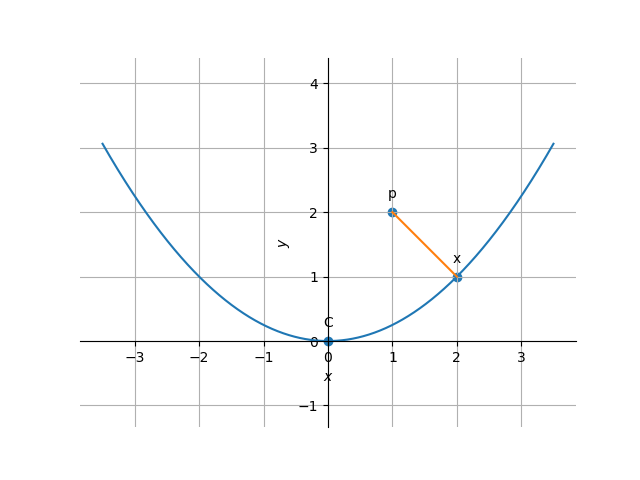
\includegraphics[scale=0.55]{opt.png}
\caption{The function f(x) with maxima and minima points}
\end{figure}        

\subsection{Calculation of Minima using gradient descent algorithm}
To find: 
\begin{align}
\min_{x} f(x)
\end{align}  
Given:
\begin{align}
f(x) = \cos^2x + \sin x,\quad x \in [0,\pi] 
\end{align}
\fi
The 
minima  is found by 
\begin{align}
	x_{n+1} &= x_n - \alpha \nabla f(x_n)
\\
 &= x_n - \alpha \brak{cosx_n-2sinx_ncosx_n}
\end{align}
\iffalse
where \\
1)$x_0=0.5$ \\
2)$\alpha=0.001$ \\
3)precision $= 0.00000001$ \\
values obtained using python are:
    \begin{align}
        \boxed{\text{Minima} = 1 }\\
        \boxed{\text{Minima Point} = 1.57}
    \end{align}

\end{document}
\fi


\end{enumerate}

\chapter{Optimization}
\section{Lagrange Multipliers}
\iffalse
\documentclass[journal,12pt,twocolumn]{IEEEtran}
\usepackage{setspace}
\usepackage{gensymb}
\usepackage{caption}
%\usepackage{multirow}
%\usepackage{multicolumn}
%\usepackage{subcaption}
%\doublespacing
\singlespacing
\usepackage{csvsimple}
\usepackage{amsmath}
\usepackage{multicol}
%\usepackage{enumerate}
\usepackage{amssymb}
%\usepackage{graphicx}
\usepackage{newfloat}
%\usepackage{syntax}
\usepackage{listings}
\usepackage{iithtlc}
\usepackage{color}
\usepackage{tikz}
\usetikzlibrary{shapes,arrows}



%\usepackage{graphicx}
%\usepackage{amssymb}
%\usepackage{relsize}
%\usepackage[cmex10]{amsmath}
%\usepackage{mathtools}
%\usepackage{amsthm}
%\interdisplaylinepenalty=2500
%\savesymbol{iint}
%\usepackage{txfonts}
%\restoresymbol{TXF}{iint}
%\usepackage{wasysym}
\usepackage{amsthm}
\usepackage{mathrsfs}
\usepackage{txfonts}
\usepackage{stfloats}
\usepackage{cite}
\usepackage{cases}
\usepackage{mathtools}
\usepackage{caption}
\usepackage{enumerate}	
\usepackage{enumitem}
\usepackage{amsmath}
%\usepackage{xtab}
\usepackage{longtable}
\usepackage{multirow}
%\usepackage{algorithm}
%\usepackage{algpseudocode}
\usepackage{enumitem}
\usepackage{mathtools}
\usepackage{hyperref}
%\usepackage[framemethod=tikz]{mdframed}
\usepackage{listings}
    %\usepackage[latin1]{inputenc}                                 %%
    \usepackage{color}                                            %%
    \usepackage{array}                                            %%
    \usepackage{longtable}                                        %%
    \usepackage{calc}                                             %%
    \usepackage{multirow}                                         %%
    \usepackage{hhline}                                           %%
    \usepackage{ifthen}                                           %%
  %optionally (for landscape tables embedded in another document): %%
    \usepackage{lscape}     


\usepackage{url}
\def\UrlBreaks{\do\/\do-}


%\usepackage{stmaryrd}


%\usepackage{wasysym}
%\newcounter{MYtempeqncnt}
\DeclareMathOperator*{\Res}{Res}
%\renewcommand{\baselinestretch}{2}
\renewcommand\thesection{\arabic{section}}
\renewcommand\thesubsection{\thesection.\arabic{subsection}}
\renewcommand\thesubsubsection{\thesubsection.\arabic{subsubsection}}

\renewcommand\thesectiondis{\arabic{section}}
\renewcommand\thesubsectiondis{\thesectiondis.\arabic{subsection}}
\renewcommand\thesubsubsectiondis{\thesubsectiondis.\arabic{subsubsection}}

% correct bad hyphenation here
\hyphenation{op-tical net-works semi-conduc-tor}

%\lstset{
%language=C,
%frame=single, 
%breaklines=true
%}

%\lstset{
	%%basicstyle=\small\ttfamily\bfseries,
	%%numberstyle=\small\ttfamily,
	%language=Octave,
	%backgroundcolor=\color{white},
	%%frame=single,
	%%keywordstyle=\bfseries,
	%%breaklines=true,
	%%showstringspaces=false,
	%%xleftmargin=-10mm,
	%%aboveskip=-1mm,
	%%belowskip=0mm
%}

%\surroundwithmdframed[width=\columnwidth]{lstlisting}
\def\inputGnumericTable{}                                 %%
\lstset{
%language=C,
frame=single, 
breaklines=true,
columns=fullflexible
}
 

\begin{document}
%
\tikzstyle{block} = [rectangle, draw,
    text width=3em, text centered, minimum height=3em]
\tikzstyle{sum} = [draw, circle, node distance=3cm]
\tikzstyle{input} = [coordinate]
\tikzstyle{output} = [coordinate]
\tikzstyle{pinstyle} = [pin edge={to-,thin,black}]

\theoremstyle{definition}
\newtheorem{theorem}{Theorem}[section]
\newtheorem{problem}{Problem}
\newtheorem{proposition}{Proposition}[section]
\newtheorem{lemma}{Lemma}[section]
\newtheorem{corollary}[theorem]{Corollary}
\newtheorem{example}{Example}[section]
\newtheorem{definition}{Definition}[section]
%\newtheorem{algorithm}{Algorithm}[section]
%\newtheorem{cor}{Corollary}
\newcommand{\BEQA}{\begin{eqnarray}}
\newcommand{\EEQA}{\end{eqnarray}}
\newcommand{\define}{\stackrel{\triangle}{=}}

\bibliographystyle{IEEEtran}
%\bibliographystyle{ieeetr}

\providecommand{\nCr}[2]{\,^{#1}C_{#2}} % nCr
\providecommand{\nPr}[2]{\,^{#1}P_{#2}} % nPr
\providecommand{\mbf}{\mathbf}
\providecommand{\pr}[1]{\ensuremath{\Pr\left(#1\right)}}
\providecommand{\qfunc}[1]{\ensuremath{Q\left(#1\right)}}
\providecommand{\sbrak}[1]{\ensuremath{{}\left[#1\right]}}
\providecommand{\lsbrak}[1]{\ensuremath{{}\left[#1\right.}}
\providecommand{\rsbrak}[1]{\ensuremath{{}\left.#1\right]}}
\providecommand{\brak}[1]{\ensuremath{\left(#1\right)}}
\providecommand{\lbrak}[1]{\ensuremath{\left(#1\right.}}
\providecommand{\rbrak}[1]{\ensuremath{\left.#1\right)}}
\providecommand{\cbrak}[1]{\ensuremath{\left\{#1\right\}}}
\providecommand{\lcbrak}[1]{\ensuremath{\left\{#1\right.}}
\providecommand{\rcbrak}[1]{\ensuremath{\left.#1\right\}}}
\theoremstyle{remark}
\newtheorem{rem}{Remark}
\newcommand{\sgn}{\mathop{\mathrm{sgn}}}
\providecommand{\abs}[1]{\left\vert#1\right\vert}
\providecommand{\res}[1]{\Res\displaylimits_{#1}} 
\providecommand{\norm}[1]{\left\Vert#1\right\Vert}
\providecommand{\mtx}[1]{\mathbf{#1}}
\providecommand{\mean}[1]{E\left[ #1 \right]}
\providecommand{\fourier}{\overset{\mathcal{F}}{ \rightleftharpoons}}
%\providecommand{\hilbert}{\overset{\mathcal{H}}{ \rightleftharpoons}}
\providecommand{\system}{\overset{\mathcal{H}}{ \longleftrightarrow}}
	%\newcommand{\solution}[2]{\textbf{Solution:}{#1}}
\newcommand{\solution}{\noindent \textbf{Solution: }}
\newcommand{\myvec}[1]{\ensuremath{\begin{pmatrix}#1\end{pmatrix}}}
\providecommand{\dec}[2]{\ensuremath{\overset{#1}{\underset{#2}{\gtrless}}}}
\DeclarePairedDelimiter{\ceil}{\lceil}{\rceil}
%\numberwithin{equation}{section}
%\numberwithin{problem}{subsection}
%\numberwithin{definition}{subsection}
\makeatletter
\@addtoreset{figure}{section}
\makeatother

\let\StandardTheFigure\thefigure
%\renewcommand{\thefigure}{\theproblem.\arabic{figure}}
\renewcommand{\thefigure}{\thesection}


%\numberwithin{figure}{subsection}

%\numberwithin{equation}{subsection}
%\numberwithin{equation}{section}
%\numberwithin{equation}{problem}
%\numberwithin{problem}{subsection}
\numberwithin{problem}{section}
%%\numberwithin{definition}{subsection}
%\makeatletter
%\@addtoreset{figure}{problem}
%\makeatother
\makeatletter
\@addtoreset{table}{section}
\makeatother

\let\StandardTheFigure\thefigure
\let\StandardTheTable\thetable
\let\vec\mathbf
%%\renewcommand{\thefigure}{\theproblem.\arabic{figure}}
%\renewcommand{\thefigure}{\theproblem}

%%\numberwithin{figure}{section}

%%\numberwithin{figure}{subsection}


%\documentclass[journal,12pt,twocolumn]{IEEEtran}
%%
%\usepackage{setspace}
%\usepackage{gensymb}
%\usepackage{xcolor}
%\usepackage{caption}
%%\usepackage{subcaption}
%%\doublespacing
%\singlespacing
%\usepackage{enumitem}
%%\usepackage{multicol}
%%\usepackage{graphicx}
%%\usepackage{amssymb}
%%\usepackage{relsize}
%\usepackage[cmex10]{amsmath}
%\usepackage{mathtools}
%%\usepackage{amsthm}
%%\interdisplaylinepenalty=2500
%%\savesymbol{iint}
%%\usepackage{txfonts}
%%\restoresymbol{TXF}{iint}
%%\usepackage{wasysym}
%\usepackage{amsthm}
%\usepackage{mathrsfs}
%\usepackage{txfonts}
%\usepackage{stfloats}
%\usepackage{cite}
%\usepackage{cases}
%\usepackage{subfig}
%%\usepackage{xtab}
%\usepackage{longtable}
%\usepackage{multirow}
%%\usepackage{algorithm}
%%\usepackage{algpseudocode}
%\usepackage{enumitem}
%\usepackage{mathtools}
%\usepackage{iithtlc}
%%\usepackage[framemethod=tikz]{mdframed}
%\usepackage{listings}
%    \usepackage[latin1]{inputenc}                                 %%
%    \usepackage{color}                                            %%
%    \usepackage{array}                                            %%
%    \usepackage{longtable}                                        %%
%    \usepackage{calc}                                             %%
%    \usepackage{multirow}                                         %%
%    \usepackage{hhline}                                           %%
%    \usepackage{ifthen}                                           %%
%  %optionally (for landscape tables embedded in another document): %%
%    \usepackage{lscape}     
%
%%\usepackage{stmaryrd}
%
%
%%\usepackage{wasysym}
%%\newcounter{MYtempeqncnt}
%\DeclareMathOperator*{\Res}{Res}
%%\renewcommand{\baselinestretch}{2}
%\renewcommand\thesection{\arabic{section}}
%\renewcommand\thesubsection{\thesection.\arabic{subsection}}
%\renewcommand\thesubsubsection{\thesubsection.\arabic{subsubsection}}
%
%\renewcommand\thesectiondis{\arabic{section}}
%\renewcommand\thesubsectiondis{\thesectiondis.\arabic{subsection}}
%\renewcommand\thesubsubsectiondis{\thesubsectiondis.\arabic{subsubsection}}
%
%% correct bad hyphenation here
%\hyphenation{op-tical net-works semi-conduc-tor}
%
%\def\inputGnumericTable{}  
%
%\lstset{
%%language=python,
%frame=single, 
%breaklines=true,
%columns=fullflexible
%}
%\newcommand\bigzero{\makebox(0,0){\text{\huge0}}}
%%\lstset{
%	%%basicstyle=\small\ttfamily\bfseries,
%	%%numberstyle=\small\ttfamily,
%	%language=Octave,
%	%backgroundcolor=\color{white},
%	%%frame=single,
%	%%keywordstyle=\bfseries,
%	%%breaklines=true,
%	%%showstringspaces=false,
%	%%xleftmargin=-10mm,
%	%%aboveskip=-1mm,
%	%%belowskip=0mm
%%}
%
%%\surroundwithmdframed[width=\columnwidth]{lstlisting}
%
%
%\begin{document}
%%
%
%\theoremstyle{definition}
%\newtheorem{theorem}{Theorem}[section]
%\newtheorem{problem}{Problem}
%\newtheorem{proposition}{Proposition}[section]
%\newtheorem{lemma}{Lemma}[section]
%\newtheorem{corollary}[theorem]{Corollary}
%\newtheorem{example}{Example}[section]
%\newtheorem{definition}{Definition}[section]
%%\newtheorem{algorithm}{Algorithm}[section]
%%\newtheorem{cor}{Corollary}
%\newcommand{\BEQA}{\begin{eqnarray}}
%\newcommand{\EEQA}{\end{eqnarray}}
%\newcommand{\define}{\stackrel{\triangle}{=}}
%
%\bibliographystyle{IEEEtran}
%%\bibliographystyle{ieeetr}
%
%\providecommand{\nCr}[2]{\,^{#1}C_{#2}} % nCr
%\providecommand{\nPr}[2]{\,^{#1}P_{#2}} % nPr
%\providecommand{\mbf}{\mathbf}
%\providecommand{\pr}[1]{\ensuremath{\Pr\left(#1\right)}}
%\providecommand{\qfunc}[1]{\ensuremath{Q\left(#1\right)}}
%\providecommand{\sbrak}[1]{\ensuremath{{}\left[#1\right]}}
%\providecommand{\lsbrak}[1]{\ensuremath{{}\left[#1\right.}}
%\providecommand{\rsbrak}[1]{\ensuremath{{}\left.#1\right]}}
%\providecommand{\brak}[1]{\ensuremath{\left(#1\right)}}
%\providecommand{\lbrak}[1]{\ensuremath{\left(#1\right.}}
%\providecommand{\rbrak}[1]{\ensuremath{\left.#1\right)}}
%\providecommand{\cbrak}[1]{\ensuremath{\left\{#1\right\}}}
%\providecommand{\lcbrak}[1]{\ensuremath{\left\{#1\right.}}
%\providecommand{\rcbrak}[1]{\ensuremath{\left.#1\right\}}}
%\theoremstyle{remark}
%\newtheorem{rem}{Remark}
%\newcommand{\sgn}{\mathop{\mathrm{sgn}}}
%\providecommand{\abs}[1]{\left\vert#1\right\vert}
%\providecommand{\res}[1]{\Res\displaylimits_{#1}} 
%\providecommand{\norm}[1]{\lVert#1\rVert}
%%\providecommand{\norm}[1]{\lVert#1\rVert}
%\providecommand{\mtx}[1]{\mathbf{#1}}
%\providecommand{\mean}[1]{E\left[ #1 \right]}
%\providecommand{\fourier}{\overset{\mathcal{F}}{ \rightleftharpoons}}
%%\providecommand{\hilbert}{\overset{\mathcal{H}}{ \rightleftharpoons}}
%\providecommand{\system}{\overset{\mathcal{H}}{ \longleftrightarrow}}
%	%\newcommand{\solution}[2]{\textbf{Solution:}{#1}}
%\newcommand{\solution}{\noindent \textbf{Solution: }}
%\providecommand{\dec}[2]{\ensuremath{\overset{#1}{\underset{#2}{\gtrless}}}}
%\newcommand{\myvec}[1]{\ensuremath{\begin{pmatrix}#1\end{pmatrix}}}
%%\numberwithin{equation}{subsection}
%\numberwithin{equation}{section}
%%\numberwithin{equation}{problem}
%%\numberwithin{problem}{subsection}
%\numberwithin{problem}{section}
\numberwithin{equation}{section}
%%\numberwithin{definition}{subsection}
%\makeatletter
%\@addtoreset{figure}{problem}
%\makeatother
%\makeatletter
%\@addtoreset{table}{problem}
%\makeatother
%
%\let\StandardTheFigure\thefigure
%\let\StandardTheTable\thetable
%\let\vec\mathbf
%%\renewcommand{\thefigure}{\theproblem.\arabic{figure}}
%\renewcommand{\thefigure}{\theproblem}
%\renewcommand{\thetable}{\theproblem}
%%\numberwithin{figure}{section}
%
%%\numberwithin{figure}{subsection}
%
%\def\putbox#1#2#3{\makebox[0in][l]{\makebox[#1][l]{}\raisebox{\baselineskip}[0in][0in]{\raisebox{#2}[0in][0in]{#3}}}}
%     \def\rightbox#1{\makebox[0in][r]{#1}}
%     \def\centbox#1{\makebox[0in]{#1}}
%     \def\topbox#1{\raisebox{-\baselineskip}[0in][0in]{#1}}
%     \def\midbox#1{\raisebox{-0.5\baselineskip}[0in][0in]{#1}}

\vspace{3cm}


\title{%Convex Optimization in Python
	\logo{
	Convex Optimization in Python
	}
}
%\title{
%	\logo{Matrix Analysis through Octave}{\begin{center}\includegraphics[scale=.24]{tlc}\end{center}}{}{HAMDSP}
%}


% paper title
% can use linebreaks \\ within to get better formatting as desired
%\title{Matrix Analysis through Octave}
%
%
% author names and IEEE memberships
% note positions of commas and nonbreaking spaces ( ~ ) LaTeX will not break
% a structure at a ~ so this keeps an author's name from being broken across
% two lines.
% use \thanks{} to gain access to the first footnote area
% a separate \thanks must be used for each paragraph as LaTeX2e's \thanks
% was not built to handle multiple paragraphs
%

\author{Y Aditya, G V S S Praneeth Varma and G V V Sharma$^{*}$% <-this % stops a space
\thanks{* The authors are with the Department
of Electrical Engineering, Indian Institute of Technology, Hyderabad
502285 India e-mail:  gadepall@iith.ac.in.}% <-this % stops a space
%\thanks{J. Doe and J. Doe are with Anonymous University.}% <-this % stops a space
%\thanks{Manuscript received April 19, 2005; revised January 11, 2007.}}
}
% note the % following the last \IEEEmembership and also \thanks - 
% these prevent an unwanted space from occurring between the last author name
% and the end of the author line. i.e., if you had this:
% 
% \author{....lastname \thanks{...} \thanks{...} }
%                     ^------------^------------^----Do not want these spaces!
%
% a space would be appended to the last name and could cause every name on that
% line to be shifted left slightly. This is one of those "LaTeX things". For
% instance, "\textbf{A} \textbf{B}" will typeset as "A B" not "AB". To get
% "AB" then you have to do: "\textbf{A}\textbf{B}"
% \thanks is no different in this regard, so shield the last } of each \thanks
% that ends a line with a % and do not let a space in before the next \thanks.
% Spaces after \IEEEmembership other than the last one are OK (and needed) as
% you are supposed to have spaces between the names. For what it is worth,
% this is a minor point as most people would not even notice if the said evil
% space somehow managed to creep in.



% The paper headers
%\markboth{Journal of \LaTeX\ Class Files,~Vol.~6, No.~1, January~2007}%
%{Shell \MakeLowercase{\textit{et al.}}: Bare Demo of IEEEtran.cls for Journals}
% The only time the second header will appear is for the odd numbered pages
% after the title page when using the twoside option.
% 
% *** Note that you probably will NOT want to include the author's ***
% *** name in the headers of peer review papers.                   ***
% You can use \ifCLASSOPTIONpeerreview for conditional compilation here if
% you desire.




% If you want to put a publisher's ID mark on the page you can do it like
% this:
%\IEEEpubid{0000--0000/00\$00.00~\copyright~2007 IEEE}
% Remember, if you use this you must call \IEEEpubidadjcol in the second
% column for its text to clear the IEEEpubid mark.



% make the title area
\maketitle

\tableofcontents

\renewcommand{\thefigure}{\theenumi}
\renewcommand{\thetable}{\theenumi}

\begin{abstract}
This manual provides a simple introduction to various concepts in optimization.
\end{abstract}


%\chapter{The Optimum Receiver}
\section{Convex Functions}

%\subsection{Problem}
A single variable function $f$ is said to be convex if
%
\begin{align}
\label{ch1_convex_def}
f\sbrak{\lambda x + \brak{1-\lambda}y} \leq \lambda f\brak{x} + \brak{1-\lambda}f\brak{y}, 
\end{align}
%
for $\quad 0 < \lambda < 1$.
\begin{enumerate}[label=\thesection.\arabic*,ref=\thesection.\theenumi]

\item
Download and execute the following python script. Is  $\ln x$ convex or  concave?

%
\begin{lstlisting}[language=sh]
wget https://raw.githubusercontent.com/gadepall/optimization/master/manual/codes/1.1.py
\end{lstlisting}
%
\begin{figure}[!ht]
\centering
\includegraphics[width=\columnwidth]{./manual/figs/1.1.eps}
\caption{ $\ln x$ versus $x$}.
\label{fig.1.1}	
\end{figure}
%
\item
Modify the above python script as follows to plot the parabola $f(x) = x^2$. Is it convex or concave?

\begin{lstlisting}
wget https://raw.githubusercontent.com/gadepall/optimization/master/manual/codes/1.2.py
\end{lstlisting}
%
\begin{figure}[!ht]
\centering
\includegraphics[width=\columnwidth]{./manual/figs/1.2.eps}
\caption{ $x^2$ versus $x$}.
\label{fig.1.2}	
\end{figure}
%
\item
Execute the following script to obtain Fig. \ref{fig.1.3}. Comment.

%
\begin{lstlisting}
wget https://raw.githubusercontent.com/gadepall/optimization/master/manual/codes/1.3.py
\end{lstlisting}

%
\begin{figure}[!ht]
\centering
\includegraphics[width=\columnwidth]{./manual/figs/1.3.eps}
\caption{ Segments are below the curve}.
\label{fig.1.3}	
\end{figure}
%
\item
Modify the script in the previous problem for $f(x) = x^2$.  What can you conclude?

\item
Let 
\begin{equation}
f(\mathbf{x}) = x_1x_2, \quad \mathbf{x} \in \mathbf{R}^2
\end{equation}
Sketch $f(\mathbf{x})$ and deduce whether it is convex.
\item Show that 
\begin{equation}
f(\mathbf{x}) = \vec{x}^T\vec{V}\vec{x} 
\end{equation}
%
and find $\vec{V}$.
\item Show that 
\begin{equation}
\frac{1}{2}\nabla^2f(\mathbf{x}) = \vec{V}
\end{equation}

\item Use \eqref{ch1_convex_def} to examine the convexity of $f(\vec{x})$.
\item How can you deduce the convexity of $f(\vec{x})$ using the eigenvalues of $\vec{V}$?

\end{enumerate}
%
\section{Gradient Descent Method}
Consider the problem of finding the square root of a number $c$.  This can be expressed as the equation
%
\begin{equation}
\label{eq:root}
x^2 -c= 0
\end{equation}
%
\begin{enumerate}[label=\thesection.\arabic*,ref=\thesection.\theenumi]

\item
Sketch the function for different values of $c$
%
\begin{equation}
f(x)= x^{3}-3xc
\end{equation}
%
and comment upon its convexity.

\item
Show that \eqref{eq:root} results from
\begin{align}
\min_{x}f(x)= x^{3}-3xc
\end{align}

\item
Find a numerical solution for \eqref{eq:root}.

\solution
A numerical solution for \eqref{eq:root} is obtained as
%
\begin{align}
x_{n+1}&=x_{n}-\mu f^{\prime}\brak{x}
\\
&=x_{n} -\mu \brak{3x_n^{2}-3c}
\label{eq:gradient}
\end{align}

%\begin{align}
%x_{n+1}&=x_{n}-{\frac {f(x_{n})}{f^{\prime}(x_{n})}}
%\\
%&=x_{n} -\frac{x^2_{n}-c}{2x_n} 
%\\
%&=\frac{1}{2}\sbrak{x_{n} +\frac{c}{x_n} }
%\label{eq:newton}
%\end{align}
%
where $x_0$ is an inital guess.
%
\item
Write a program to implement \eqref{eq:gradient}.

%
\solution Download and execute
\begin{lstlisting}
manual/codes/square_root.py
\end{lstlisting}
\end{enumerate}
\fi
%\section{Convex Optimization}
%\section{Lagrange Multipliers}
\begin{enumerate}[label=\thesection.\arabic*,ref=\thesection.\theenumi]

\item
	\label{convex_code}
Find
\begin{align}
\label{eq2_1_circ}
	\min_{\mbf{x}}f\brak{\mbf{x}} = \norm{\vec{x}-\myvec{8\\6}}^2 = r^2 \\
\text{s.t.} \quad 	g\brak{\mbf{x}} = \myvec{1 & 1}\vec{x} - 9 = 0\label{eq2_1_line}
%	\quad g\brak{\mbf{x}} = x_1 + x_2 - 9 = 0
\end{align}
by plotting the circles $f\brak{\vec{x}}$
%
%\begin{equation}
% \norm{\vec{x}-\myvec{8\\6}}^2 =r^2
%%(x_1-8)^2 + (x_2-6)^2 = r^2
%\end{equation}
%
% $\mbf{x}= \myvec{x_1\\x_2}$, 
for different values of $r$ along with the line $g\brak{\mbf{x}}$.
%
%\begin{equation}
%\label{eq2_1_line}
%g\brak{\mbf{x}} = \myvec{1 & 1}\vec{x} - 9 = 0
%\end{equation} 
%
\\
\solution 
The following code plots Fig. \ref{fig.2.1}	

%	
\begin{lstlisting}
manual/codes/2.1.py
\end{lstlisting}

%
\begin{figure}[!ht]
\centering
\includegraphics[width=\columnwidth]{./manual/figs/2.1.eps}
\caption{ Finding $ \displaystyle \min_{\mbf{x}}f\brak{\mbf{x}}$}.
\label{fig.2.1}	
\end{figure}
%
\item Show that 
\begin{align}
\min r = \frac{5}{\sqrt{2}}
\end{align}
%Obtain a theoretical solution for problem \ref{convex_code} 
%%using coordinate geometry.
%
%\solution 
%From \eqref{eq2_1_line} and \eqref{eq2_1_circ}, 
%%
%\begin{align}
%r^2 & = (x_1-8)^2 + (3- x_1)^2 \\
%&= 2 x_1^2 - 22 x_1 + 73 \\
%\Rightarrow r^2 &= \frac{\brak{2x_1-11}^2 + 5^2}{2}
%\end{align}
%%
%which is minium when $x_1 = \frac{11}{2}, x_2 = \frac{7}{2}$.  The minimum value is $\frac{25}{2}$ and 
%the radius $r = \frac{5}{\sqrt{2}}$.
\item Show that 
\begin{align}
\nabla g(\vec{x}) = \myvec{1 \\ 1}
\end{align}
where
\begin{equation}
\nabla =  
\begin{pmatrix}
\frac{\partial}{\partial x_1} \\
\frac{\partial}{\partial x_2} 
\end{pmatrix}
\end{equation}

\item Show that 
\begin{align}
\nabla f(\vec{x}) = 2\cbrak{\vec{x}-\myvec{8 \\ 6}}
\end{align}
\item From Fig. \ref{fig.2.1}, show that 
\begin{align}
\label{eq:normal}
\nabla f(\vec{p}) = \lambda \nabla g(\vec{p}),
\end{align}
%
where $\vec{p}$ is the point of contact.
\item Use \eqref{eq:normal} and $\vec{g(p)}=0$ from \eqref{eq2_1_line} to obtain $\vec{p}$.
\item
\label{lagrange}
	Define 
	\begin{equation}
	\label{lagrangian}
	L\brak{\mbf{x},\lambda} = f\brak{\mbf{x}} - \lambda g\brak{\mbf{x}}%, \quad \lambda > 0
	\end{equation}
and show that $\vec{p}$ can also be obtained by 
solving the equations
%
\begin{align}
\nabla L\brak{\mbf{x},\lambda} &= 0.
\label{tangent}
\end{align}
%
What is the sign of $\lambda$?  $L$ is known as the Lagrangian and the above technique is known as the Method of Lagrange Multipliers.

\solution
%From \eqref{eq2_1_line} and \eqref{eq2_1_circ}, 
%%
%\begin{align}
%L\brak{\mbf{x},\lambda} &= (x_1-8)^2 + (x_2-6)^2 - \lambda \brak{x_1 + x_2 - 9} \\
%\Rightarrow \nabla L\brak{\mbf{x},\lambda}  & = 
%\begin{pmatrix}
%2x_1  - 16 - \lambda \\
%2x_2 - 12 - \lambda \\
%x_1 + x_2 -9
%\end{pmatrix}
%\\
%&=
%\begin{pmatrix}
%2 &0 & - 1 \\
%0 &2 & - 1 \\
%1 & 1 & 0 
%\end{pmatrix}
%\begin{pmatrix}
%x_1 \\
%x_2 \\
%\lambda
%\end{pmatrix}
%= 
%\begin{pmatrix}
%16 \\
% 12 \\
%9
%\end{pmatrix}
%=
%0 
%\\
%\Rightarrow 
%\begin{pmatrix}
%x_1 \\
%x_2 \\
%\lambda
%\end{pmatrix}
%&= 
%\begin{pmatrix}
%\frac{11}{2} \\
% \frac{7}{2} \\
%-5
%\end{pmatrix}
%\end{align}
%%
%using the following python script.  Note that this method yields the same result as the previous exercises.  Thus, $\lambda$ is negative.
%	
\begin{lstlisting}
manual/codes/2.3.py
\end{lstlisting}
\end{enumerate}
\iffalse
\subsection{Inequality Constraints}

%
\item
\label{ch2_constraint}
Modify the code in problem \ref{convex_code} to find a graphical solution for minimising
\begin{align}
f\brak{\mbf{x}} 
%= (x_1-8)^2 + (x_2-6)^2
\end{align}
with constraint
\begin{align}
%\label{convex-constraint}
g\brak{\mbf{x}} \geq 0
%= x_1 + x_2 - 9 
\end{align}

\solution 
This problem reduces to finding the radius of the smallest circle in the shaded area in Fig. \ref{fig.2.4} .  It is clear that this radius is 0.
%	
\begin{lstlisting}
wget https://raw.githubusercontent.com/gadepall/optimization/master/manual/codes/2.4.py
\end{lstlisting}

%
\begin{figure}[!ht]
\centering
\includegraphics[width=\columnwidth]{./manual/figs/2.4.eps}
\caption{ Smallest circle in the shaded region is a point.}
\label{fig.2.4}	
\end{figure}
%
\item
\label{ch2_lagrange_fail}
Now use the method of Lagrange multipliers to solve  problem \ref{ch2_constraint} and compare with the graphical solution.  Comment.

%
\solution Using the method of Lagrange multipliers, the solution is the same as the one obtained in  problem \ref{ch2_constraint}, which is different from the graphical solution.  This means that the Lagrange multipliers method cannot be applied blindly.
\item
Repeat problem \ref{ch2_lagrange_fail} by keeping 
 $\lambda=0$.   Comment.

\solution Keeping $\lambda = 0$ results in $\vec{x}=\myvec{ 8\\ 6}$, which is the correct solution.  The minimum value of $f\brak{\mbf{x}}$ without any constraints lies in the region $g\brak{\mbf{x}} = 0$.  In this case, $\lambda = 0$.  
%
%
\item
\label{ch2_constraint_border}
Find a graphical solution for minimising
\begin{align}
f\brak{\mbf{x}}
% = (x_1-8)^2 + (x_2-6)^2
\end{align}
with constraint
\begin{align}
%\label{convex-constraint}
g\brak{\mbf{x}} \leq 0
%= x_1 + x_2 - 9 .
\end{align}
Summarize your observations.

%
\solution In Fig. \ref{fig.2.7}, the shaded region represents the constraint.  Thus, the solution is the same as the one in problem \ref{ch2_constraint}. This implies that the method of
Lagrange multipliers can be used to solve the optimization problem with this inequality constraint as well.  Table \ref{table.2.7} summarizes the conditions for this based on the observations so far.
\begin{lstlisting}
wget https://raw.githubusercontent.com/gadepall/optimization/master/manual/codes/2.7.py
\end{lstlisting}

%
\begin{figure}[!ht]
\centering
\includegraphics[width=\columnwidth]{./manual/figs/2.7.eps}
\caption{ Finding $ \displaystyle \min_{\mbf{x}}f\brak{\mbf{x}}$.}
\label{fig.2.7}	
\end{figure}
%%%%%%%%%%%%%%%%%%%%%%%%%%%%%%%%%%%%%%%%%%%%%%%%%%%%%%%%%%%%%%%%%%%%%%
%%                                                                  %%
%%  This is the header of a LaTeX2e file exported from Gnumeric.    %%
%%                                                                  %%
%%  This file can be compiled as it stands or included in another   %%
%%  LaTeX document. The table is based on the longtable package so  %%
%%  the longtable options (headers, footers...) can be set in the   %%
%%  preamble section below (see PRAMBLE).                           %%
%%                                                                  %%
%%  To include the file in another, the following two lines must be %%
%%  in the including file:                                          %%
%%        \def\inputGnumericTable{}                                 %%
%%  at the beginning of the file and:                               %%
%%        \input{name-of-this-file.tex}                             %%
%%  where the table is to be placed. Note also that the including   %%
%%  file must use the following packages for the table to be        %%
%%  rendered correctly:                                             %%
%%    \usepackage[latin1]{inputenc}                                 %%
%%    \usepackage{color}                                            %%
%%    \usepackage{array}                                            %%
%%    \usepackage{longtable}                                        %%
%%    \usepackage{calc}                                             %%
%%    \usepackage{multirow}                                         %%
%%    \usepackage{hhline}                                           %%
%%    \usepackage{ifthen}                                           %%
%%  optionally (for landscape tables embedded in another document): %%
%%    \usepackage{lscape}                                           %%
%%                                                                  %%
%%%%%%%%%%%%%%%%%%%%%%%%%%%%%%%%%%%%%%%%%%%%%%%%%%%%%%%%%%%%%%%%%%%%%%



%%  This section checks if we are begin input into another file or  %%
%%  the file will be compiled alone. First use a macro taken from   %%
%%  the TeXbook ex 7.7 (suggestion of Han-Wen Nienhuys).            %%
\def\ifundefined#1{\expandafter\ifx\csname#1\endcsname\relax}


%%  Check for the \def token for inputed files. If it is not        %%
%%  defined, the file will be processed as a standalone and the     %%
%%  preamble will be used.                                          %%
\ifundefined{inputGnumericTable}

%%  We must be able to close or not the document at the end.        %%
	\def\gnumericTableEnd{\end{document}}


%%%%%%%%%%%%%%%%%%%%%%%%%%%%%%%%%%%%%%%%%%%%%%%%%%%%%%%%%%%%%%%%%%%%%%
%%                                                                  %%
%%  This is the PREAMBLE. Change these values to get the right      %%
%%  paper size and other niceties.                                  %%
%%                                                                  %%
%%%%%%%%%%%%%%%%%%%%%%%%%%%%%%%%%%%%%%%%%%%%%%%%%%%%%%%%%%%%%%%%%%%%%%

	\documentclass[12pt%
			  %,landscape%
                    ]{report}
       \usepackage[latin1]{inputenc}
       \usepackage{fullpage}
       \usepackage{color}
       \usepackage{array}
       \usepackage{longtable}
       \usepackage{calc}
       \usepackage{multirow}
       \usepackage{hhline}
       \usepackage{ifthen}

	\begin{document}


%%  End of the preamble for the standalone. The next section is for %%
%%  documents which are included into other LaTeX2e files.          %%
\else

%%  We are not a stand alone document. For a regular table, we will %%
%%  have no preamble and only define the closing to mean nothing.   %%
    \def\gnumericTableEnd{}

%%  If we want landscape mode in an embedded document, comment out  %%
%%  the line above and uncomment the two below. The table will      %%
%%  begin on a new page and run in landscape mode.                  %%
%       \def\gnumericTableEnd{\end{landscape}}
%       \begin{landscape}


%%  End of the else clause for this file being \input.              %%
\fi

%%%%%%%%%%%%%%%%%%%%%%%%%%%%%%%%%%%%%%%%%%%%%%%%%%%%%%%%%%%%%%%%%%%%%%
%%                                                                  %%
%%  The rest is the gnumeric table, except for the closing          %%
%%  statement. Changes below will alter the table's appearance.     %%
%%                                                                  %%
%%%%%%%%%%%%%%%%%%%%%%%%%%%%%%%%%%%%%%%%%%%%%%%%%%%%%%%%%%%%%%%%%%%%%%

\providecommand{\gnumericmathit}[1]{#1} 
%%  Uncomment the next line if you would like your numbers to be in %%
%%  italics if they are italizised in the gnumeric table.           %%
%\renewcommand{\gnumericmathit}[1]{\mathit{#1}}
\providecommand{\gnumericPB}[1]%
{\let\gnumericTemp=\\#1\let\\=\gnumericTemp\hspace{0pt}}
 \ifundefined{gnumericTableWidthDefined}
        \newlength{\gnumericTableWidth}
        \newlength{\gnumericTableWidthComplete}
        \newlength{\gnumericMultiRowLength}
        \global\def\gnumericTableWidthDefined{}
 \fi
%% The following setting protects this code from babel shorthands.  %%
 \ifthenelse{\isundefined{\languageshorthands}}{}{\languageshorthands{english}}
%%  The default table format retains the relative column widths of  %%
%%  gnumeric. They can easily be changed to c, r or l. In that case %%
%%  you may want to comment out the next line and uncomment the one %%
%%  thereafter                                                      %%
\providecommand\gnumbox{\makebox[0pt]}
%%\providecommand\gnumbox[1][]{\makebox}

%% to adjust positions in multirow situations                       %%
\setlength{\bigstrutjot}{\jot}
\setlength{\extrarowheight}{\doublerulesep}

%%  The \setlongtables command keeps column widths the same across  %%
%%  pages. Simply comment out next line for varying column widths.  %%
\setlongtables

\setlength\gnumericTableWidth{%
	53pt+%
	58pt+%
	55pt+%
0pt}
\def\gumericNumCols{3}
\setlength\gnumericTableWidthComplete{\gnumericTableWidth+%
         \tabcolsep*\gumericNumCols*2+\arrayrulewidth*\gumericNumCols}
\ifthenelse{\lengthtest{\gnumericTableWidthComplete > \linewidth}}%
         {\def\gnumericScale{\ratio{\linewidth-%
                        \tabcolsep*\gumericNumCols*2-%
                        \arrayrulewidth*\gumericNumCols}%
{\gnumericTableWidth}}}%
{\def\gnumericScale{1}}

%%%%%%%%%%%%%%%%%%%%%%%%%%%%%%%%%%%%%%%%%%%%%%%%%%%%%%%%%%%%%%%%%%%%%%
%%                                                                  %%
%% The following are the widths of the various columns. We are      %%
%% defining them here because then they are easier to change.       %%
%% Depending on the cell formats we may use them more than once.    %%
%%                                                                  %%
%%%%%%%%%%%%%%%%%%%%%%%%%%%%%%%%%%%%%%%%%%%%%%%%%%%%%%%%%%%%%%%%%%%%%%

\ifthenelse{\isundefined{\gnumericColA}}{\newlength{\gnumericColA}}{}\settowidth{\gnumericColA}{\begin{tabular}{@{}p{53pt*\gnumericScale}@{}}x\end{tabular}}
\ifthenelse{\isundefined{\gnumericColB}}{\newlength{\gnumericColB}}{}\settowidth{\gnumericColB}{\begin{tabular}{@{}p{58pt*\gnumericScale}@{}}x\end{tabular}}
\ifthenelse{\isundefined{\gnumericColC}}{\newlength{\gnumericColC}}{}\settowidth{\gnumericColC}{\begin{tabular}{@{}p{55pt*\gnumericScale}@{}}x\end{tabular}}

\begin{table}[!h]
	\caption{Summary of conditions.} 
	\centering
\begin{tabular}[c]{%
	b{\gnumericColA}%
	b{\gnumericColB}%
	b{\gnumericColC}%
	}

%%%%%%%%%%%%%%%%%%%%%%%%%%%%%%%%%%%%%%%%%%%%%%%%%%%%%%%%%%%%%%%%%%%%%%
%%  The longtable options. (Caption, headers... see Goosens, p.124) %%            \\	%
 %\hline	% Across the top of the table.
%%  The rest of these options are table rows which are placed on    %%
%%  the first, last or every page. Use \multicolumn if you want.    %%

%%  Header for the first page.                                      %%
%	\multicolumn{3}{c}{The First Header} \\ \hline 
%	\multicolumn{1}{c}{colTag}	%Column 1
%	&\multicolumn{1}{c}{colTag}	%Column 2
%	&\multicolumn{1}{c}{colTag}	\\ \hline %Last column
%	\endfirsthead

%%  The running header definition.                                  %%
%	\hline
%	\multicolumn{3}{l}{\ldots\small\slshape continued} \\ \hline
%	\multicolumn{1}{c}{colTag}	%Column 1
%	&\multicolumn{1}{c}{colTag}	%Column 2
%	&\multicolumn{1}{c}{colTag}	\\ \hline %Last column
%	\endhead

%%  The running footer definition.                                  %%
%	\hline
%	\multicolumn{3}{r}{\small\slshape continued\ldots} \\
%	\endfoot

%%  The ending footer definition.                                   %%
%	\multicolumn{3}{c}{That's all folks} \\ \hline 
%	\endlastfoot
%%%%%%%%%%%%%%%%%%%%%%%%%%%%%%%%%%%%%%%%%%%%%%%%%%%%%%%%%%%%%%%%%%%%%%

\hhline{|-|-|-}
	 \multicolumn{1}{|p{\gnumericColA}|}%
	{\gnumericPB{\centering}\textbf{Cost}}
	&\multicolumn{1}{p{\gnumericColB}|}%
	{\gnumericPB{\centering}\textbf{Constraint}}
	&\multicolumn{1}{p{\gnumericColC}|}%
	{\gnumericPB{\centering}\textbf{$\lambda$}}
\\
\hhline{|---|}
	 \multicolumn{1}{|p{\gnumericColA}|}%
	{\setlength{\gnumericMultiRowLength}{0pt}%
	 \addtolength{\gnumericMultiRowLength}{\gnumericColA}%
	 \multirow{3}[1]{\gnumericMultiRowLength}{\parbox{\gnumericMultiRowLength}{%
	 \gnumericPB{\centering}$f\brak{\mbf{x}}$}}}
	&\multicolumn{1}{p{\gnumericColB}|}%
	{\gnumericPB{\centering}$g\brak{\mbf{x}} = 0$}
	&\multicolumn{1}{p{\gnumericColC}|}%
	{\gnumericPB{\centering} $<$ 0}
\\
\hhline{~|--|}
	 \multicolumn{1}{|p{\gnumericColA}|}%
	{}
	&\multicolumn{1}{p{\gnumericColB}|}%
	{\gnumericPB{\centering}$g\brak{\mbf{x}} \geq 0 $}
	&\multicolumn{1}{p{\gnumericColC}|}%
	{\gnumericPB{\centering}0}
\\
\hhline{~|--|}
	 \multicolumn{1}{|p{\gnumericColA}|}%
	{}
	&\multicolumn{1}{p{\gnumericColB}|}%
	{\gnumericPB{\centering}$g\brak{\mbf{x}}\leq 0 $}
	&\multicolumn{1}{p{\gnumericColC}|}%
	{\gnumericPB{\centering} $<$ 0}
\\
\hhline{|-|-|-|}
\end{tabular}
\label{table.2.7}
\end{table}

\ifthenelse{\isundefined{\languageshorthands}}{}{\languageshorthands{\languagename}}
\gnumericTableEnd

%
\item
\label{ch2_prob_upper}
Find a graphical solution for 	 
	 \begin{align}
	 \label{ch2_second_min}
	\min_{\mbf{x}} f\brak{\mbf{x}} = \norm{\vec{x}-\myvec{8\\6}}^2
	 \end{align}
	 with constraint
	 \begin{align}
	 \label{ch2_second_const}
	 g\brak{\mbf{x}} = \myvec{1 & 1}\vec{x} - 18 = 0
	 \end{align}
	 
%
\solution
%	
\begin{lstlisting}
wget https://raw.githubusercontent.com/gadepall/optimization/master/manual/codes/2.8.py
\end{lstlisting}

%
\begin{figure}[!ht]
\centering
\includegraphics[width=\columnwidth]{./manual/figs/2.8.eps}
\caption{ Finding $ \displaystyle \min_{\mbf{x}}f\brak{\mbf{x}}$.}
\label{fig.2.8}	
\end{figure}
%
\item
Repeat problem \ref{ch2_prob_upper} using the method of Lagrange mutipliers.  What is the sign of $\lambda$?

%
\solution
%From \eqref{ch2_second_min} and \eqref{ch2_second_const}, 
%%
%\begin{align}
%L\brak{\mbf{x},\lambda} &= (x_1-8)^2 + (x_2-6)^2 - \lambda \brak{x_1 + x_2 - 18} \\
%\Rightarrow \nabla L\brak{\mbf{x},\lambda}  & = 
%\begin{pmatrix}
%2x_1  - 16 - \lambda \\
%2x_2 - 12 - \lambda \\
%x_1 + x_2 -18
%\end{pmatrix}
%\\
%&=
%\begin{pmatrix}
%2 &0 & - 1 \\
%0 &2 & - 1 \\
%1 & 1 & 0 
%\end{pmatrix}
%\begin{pmatrix}
%x_1 \\
%x_2 \\
%\lambda
%\end{pmatrix}
%= 
%\begin{pmatrix}
%16 \\
% 12 \\
%18
%\end{pmatrix}
%=
%0 
%\\
%\Rightarrow 
%\begin{pmatrix}
%x_1 \\
%x_2 \\
%\lambda
%\end{pmatrix}
%&= 
%\begin{pmatrix}
%10 \\
% 8 \\
%4
%\end{pmatrix}
%\end{align}
%%
Using the following python script, $\lambda$ is positive and the minimum value of $f$ is 8.
%	
\begin{lstlisting}
wget https://raw.githubusercontent.com/gadepall/optimization/master/manual/codes/2.9.py
\end{lstlisting}

%
%
\item
\label{ch2_prob_upper_cond}
Solve
	 \begin{align}
%	 \label{ch2_second_min}
	\min_{\mbf{x}} f\brak{\mbf{x}} 
%= (x_1-8)^2 + (x_2-6)^2
	 \end{align}
	 with constraint
	 \begin{align}
%	 \label{ch2_second_const}
	 g\brak{\mbf{x}} 
%= x_1 + x_2 - 18 
\geq 0 
	 \end{align}
	 
%
\solution Since the unconstrained solution is outside the region $g\brak{\mbf{x}} \geq 0$, the solution is the same as the one in problem \ref{ch2_prob_upper}.
%
\item
Based on the problems so far, generalise the Lagrange multipliers method for 
%
	 \begin{align}
	 \label{ch2_lagrange_ineq}
	\min_{\mbf{x}} f\brak{\mbf{x}} , \quad 
	 g\brak{\mbf{x}}  \geq 0 
	 \end{align}
%

%
\solution
Considering $L\brak{\mbf{x},\lambda} = f\brak{\mbf{x}} - \lambda g\brak{\mbf{x}}$, for $g\brak{\mbf{x}} = \myvec{1 & 1}\vec{x} - 18 \geq 0$ we found $\lambda > 0 $ and for $g\brak{\mbf{x}} = \myvec{1 & 1}\vec{x} - 9 \leq 0, \lambda < 0$. A single condition can be obtained by framing the optimization problem as
%
	 \begin{align}
	 \label{ch2_lagrange_ineq_summary}
	\min_{\mbf{x}} f\brak{\mbf{x}} , \quad 
	 g\brak{\mbf{x}}  \leq 0 
	 \end{align}
%
with the Lagrangian
%
\begin{equation}
%\label{ch2_kkt_necessary}
L\brak{\mbf{x},\lambda} = f\brak{\mbf{x}} + \lambda g\brak{\mbf{x}}, %\quad  \lambda > 0,  g\brak{\mbf{x}} \leq 0.
\end{equation}
%
provided
%
\begin{equation}
\label{ch2_kkt_necessary}
\nabla L\brak{\mbf{x},\lambda} = 0 \Rightarrow \lambda > 0
\end{equation}
else, $\lambda = 0$.
\subsection{Karush Kuhn-Tucker Conditions}
\item
Solve
 \begin{align}
 \label{ch2_kkt_problem}
\min_{\mbf{x}} f\brak{\mbf{x}} = \vec{x}^T\myvec{4 & 0 \\0 & 2}\vec{x}
%4x_1^2 + 2x_2^2
 \end{align}
 with constraints
 \begin{align}
 g_1\brak{\mbf{x}} = \myvec{3 & 1}\vec{x}-8 = 0\\
 g_2 \brak{\mbf{x}}= 15 - \myvec{2 & 4}\vec{x} \geq 0
 \end{align}
 
%
\solution Considering the Lagrangian
%
\begin{align}
%L\brak{\mbf{x},\lambda} &= f\brak{\mbf{x}} + \lambda g_1\brak{\mbf{x}} - \mu g_2\brak{\mbf{x}} \\
% &= 4x_1^2 + 2x_2^2 + \lambda \brak{3x_1 + x_2-8} 
% \nonumber \\
% &\,-\mu\brak{15 - 2x_1 - 4x_2},\\
 \nabla L\brak{\mbf{x},\lambda, \mu}  %& = 
%\begin{pmatrix}
%8x_1 + 3 \lambda  +2 \mu  \\
%4x_2 + \lambda + 4 \mu \\
%3x_1 + x_2 -8 \\
% - 2x_1 - 4x_2 + 15
%\end{pmatrix}
= 0
\end{align}
%
resulting in the matrix equation
%
\begin{align}
\Rightarrow 
\begin{pmatrix}
8 &0 & 3 & 2\\
0 &4 & 1 & 4 \\
3 & 1 & 0 &0  \\
2 & 4 & 0 & 0
\end{pmatrix}
\begin{pmatrix}
x_1 \\
x_2 \\
\lambda
\\
\mu
\end{pmatrix}
&=
\begin{pmatrix}
0 \\
0 \\
8 \\
15
\end{pmatrix}
\\
\Rightarrow 
\begin{pmatrix}
x_1 \\
x_2 \\
\lambda
\\
\mu
\end{pmatrix}
&= 
\begin{pmatrix}
1.7 \\
 2.9 \\
-3.12 \\
-2.12
\end{pmatrix}
\end{align}
%
using the following python script.  The (incorrect) graphical solution is available in Fig. \ref{fig.2.12}
%	
\begin{lstlisting}
wget https://raw.githubusercontent.com/gadepall/optimization/master/manual/codes/2.12.py
\end{lstlisting}

%
Note that $\mu < 0 $, contradicting the necessary condition in \eqref{ch2_kkt_necessary}. 
%
\begin{figure}[!ht]
\centering
\includegraphics[width=\columnwidth]{./manual/figs/2.12_1.eps}
\caption{ Incorrect solution is at intersection of all curves $r = 5.33$}
\label{fig.2.12}	
\end{figure}
\item
Obtain the correct solution to the previous problem by considering $\mu = 0$.

\begin{figure}[!ht]
\centering
\includegraphics[width=\columnwidth]{./manual/figs/2.12_2.eps}
\caption{ Optimal solution is where $g_1(x)$ touches the curve $r = 4.82$}
\label{fig.2.13}	
\end{figure}
%
%
\item
Solve
 \begin{align}
% \label{ch2_kkt_problem}
\min_{\mbf{x}} f\brak{\mbf{x}} %= 4x_1^2 + 2x_2^2
 \end{align}
 with constraints
 \begin{align}
 g_1\brak{\mbf{x}} 
%= 3x_1 + x_2-8 
= 0\\
 g_2 \brak{\mbf{x}}
%= 15 - 2x_1 - 4x_2 
\leq 0
 \end{align}
 
%
\item
Based on whatever you have done so far,	list the steps that you would use in general for solving a convex optimization problem  like \eqref{ch2_kkt_problem}  using Lagrange Multipliers. 
These are called Karush-Kuhn-Tucker(KKT) conditions.

\solution For a problem defined by 
\begin{align}
\mbf{x^*} &= \min_{\mbf{x}}f(\mbf{x})
\\
\text{subject to } h_i(\mbf{x}) &= 0, \forall i=1,..,m
\\
\text{subject to } g_i(\mbf{x}) &\le 0, \forall i=1,..,n
\end{align}
%
the optimal solution is obtained through
%
\begin{align}
\mbf{x^*} &= \min_{\mbf{x}}L(\mbf{x}, \mbf{\lambda}, \mbf{\mu}) 
\\
&= \min_{\mbf{x}}f(\mbf{x})  + \underset{i=1}{\overset{m}{\sum}} \lambda_i h_i(\mbf{x}) + \underset{i=1}{\overset{n}{\sum}} \mu_i g_i(\mbf{x}),
\end{align}
%
using the KKT conditions
%
\begin{align}
\Rightarrow \nabla_\mbf{x} f(\mbf{x})  + \underset{i=1}{\overset{m}{\sum}} \nabla_\mbf{x} \lambda_i h_i(\mbf{x}) + \underset{i=1}{\overset{n}{\sum}} \mu_i \nabla_\mbf{x} g_i(\mbf{x}) = 0 
\\
\text{subject to }\mu_i g_i(\mbf{x}) = 0, \forall i = 1,..,n
\\
\text{and }\mu_i \ge 0, \forall i = 1,..,n
\end{align}
%
\item
	Maxmimize 
	%
	\begin{align}
	f(\mbf{x}) &= \sqrt{x_1x_2}
	\end{align}
	%
	with the constraints
	%
	\begin{align}
	x_1^2+x_2^2 &\leq 5 \\
	x_1 \geq 0, x_2 &\geq 0
	\end{align}
	%

%
\item
	\label{convex_sdp_eqiv}
	%
	Solve
	\begin{equation}
	\min_{\mbf{x}} \quad x_1 + x_2
	\end{equation}
	%	
	with the constraints
	\begin{equation}
	x_1^2 - x_1 + x_2^2 \leq 0
	\end{equation}
	%
where 
$
\mbf{x} = \begin{pmatrix}
x_1 \\
x_2
\end{pmatrix}
$

\solution 
%Using the method of Lagrange multipliers,
%%
%\begin{align}
%\label{ch2_sd_kkt}
%\nabla \cbrak{f(\mbf{x})  +  \mu g(\mbf{x}) }= 0 , \quad \mu \ge 0
%\end{align}
%%
%resulting in the equations
%%
%\begin{align}
%2x_1\mu -\mu + 1 &= 0 \\
%2x_2\mu + 1 &=0 \\
%x_1^2 -x_1 + x_2^2 &= 0 
%\end{align}
%%
%which can be simplified to obtain 
%%
%\begin{align}
%\brak{\frac{1-\mu}{2\mu}}^2 + \brak{\frac{1}{2\mu}}^2 + \frac{1-\mu}{2\mu} &= 0 \\
%\Rightarrow 1 + \mu^2 -2\mu + 1 + 2\mu\brak{1-\mu} &= 0 \\
%\Rightarrow \mu^2 =2, or \mu &= \pm \sqrt{2} 
%\end{align}
%%
%From \eqref{ch2_kkt_problem},  $\mu \ge 0 \Rightarrow  \mu = \sqrt{2}$. The desired solution is
%%
%\begin{equation}
%\mbf{x} = 
%\begin{pmatrix}
% \frac{\sqrt{2}-1}{2\sqrt{2}} \\
%-\frac{1}{2\sqrt{2}} 
%\end{pmatrix}
%\end{equation}
%
\\
{\em Graphical solution:} 
%The constraint can be expressed as
%%
%\begin{align}
%x_1^2 - x_1 + x_2^2 &\le 0 \\
%\Rightarrow \brak{x_1 - \frac{1}{2}}^2 + x_2^2 & \le \brak{\frac{1}{2}}^2
%\end{align}
%
%	
\begin{lstlisting}
wget https://raw.githubusercontent.com/gadepall/optimization/master/manual/codes/2.15.py
\end{lstlisting}

%
%
\begin{figure}[!ht]
\centering
\includegraphics[width=\columnwidth]{./manual/figs/2.15.eps}
\caption{ Optimal solution is the lower tangent to the circle}
\label{fig.2.15}	
\end{figure}
%
\end{enumerate}

\section{Semi-definite Programming}
\begin{enumerate}[label=\thesection.\arabic*,ref=\thesection.\theenumi]

%\subsection{Karush Kuhn-Tucker Conditions}

\item
%
\label{ch3_convex_ch2}
The problem
\begin{equation}
\min_{\mbf{X}} x_{11} + x_{12}
\end{equation}
%	
with constraints
\begin{align}
x_{11} + x_{22} &= 1 \\	
\mbf{X}
& \succeq 0 \quad  \brak{\text{$\succeq$ means positive definite}}
\end{align}
%
where
\begin{equation}
\mbf{X}=
\begin{pmatrix}
x_{11} & x_{12} \\
x_{12} & x_{22}
\end{pmatrix} 
\end{equation}
%
is known as a semi-definite program.  Find a numerical solution to this problem. Compare with the solution 
in problem  \ref{convex_sdp_eqiv}.
\label{prob:cvxopt}

\solution The {\em cvxopt} solver needs to be used in order to find a numerical solution.  For this, the given problem has to be reformulated as
\begin{align}
&\min_{\mbf{x}}  
\begin{pmatrix}
1 & 1 & 0
\end{pmatrix}
\begin{pmatrix}
x_{11} 
\\
x_{12}
\\
x_{22}
\end{pmatrix}
\quad \text{s.t}
\\
&
\begin{pmatrix}
1 & 0 & 1
\end{pmatrix}
\begin{pmatrix}
x_{11} 
\\
x_{12}
\\
x_{22}
\end{pmatrix}
=1
\end{align}
\begin{multline}
x_{11}
\begin{pmatrix}
-1 & 0 
\\
0 & 0
\end{pmatrix}
+
x_{12}
\begin{pmatrix}
0 & -1
\\
-1 & 0
\end{pmatrix}
+x_{22}
\begin{pmatrix}
0 & 0 
\\
0 & -1
\end{pmatrix}
\\
\preceq 
\begin{pmatrix}
0 & 0 
\\
0 & 0
\end{pmatrix}.
\end{multline}
%
The following script provides the solution to this problem.
\begin{lstlisting}
wget https://raw.githubusercontent.com/gadepall/optimization/master/manual/codes/3.1.py
\end{lstlisting}
%
\item
Frame Problem \ref{prob:cvxopt} in terms of matrices.

\solution
It is easy to verify that
\begin{equation}
x_{11} + x_{12} = 
\begin{pmatrix}
1 & 1
\end{pmatrix}
\mbf{X}^{T}
\begin{pmatrix}
1 
\\
0
\end{pmatrix}
\end{equation}
and
\begin{equation}
x_{11} + x_{22} = 
\begin{pmatrix}
1 & 0 & 0 & 1
\end{pmatrix}
\begin{pmatrix}
\mbf{X} & \mbf{0} \\
\mbf{0} & \mbf{X}
\end{pmatrix}
\begin{pmatrix}
1
\\
0 
\\
0
\\
1
\end{pmatrix}
\end{equation}
%
Thus, Problem \ref{prob:cvxopt} can be expressed as
\begin{equation}
\begin{split}
\min_{\mbf{X}} 
\begin{pmatrix}
1 & 1
\end{pmatrix}
\mbf{X}^{T}
\begin{pmatrix}
1 
\\
0
\end{pmatrix}
& \quad s.t
\\
\begin{pmatrix}
1 & 0 & 0 & 1
\end{pmatrix}
\begin{pmatrix}
\mbf{X} & \mbf{0} \\
\mbf{0} & \mbf{X}
\end{pmatrix}
\begin{pmatrix}
1
\\
0 
\\
0
\\
1
\end{pmatrix}
&=1,
\\
\mbf{X}
 & \succeq 0 
\end{split}
\label{prob:cvxpy}
\end{equation}
%	
\item
Solve \eqref{prob:cvxpy} using {\em cvxpy}.

%
\solution
\begin{lstlisting}
wget https://raw.githubusercontent.com/gadepall/optimization/master/manual/codes/3.1-cvx.py
\end{lstlisting}

\item
Minimize 
\begin{equation}
-x_{11} - 2x_{12} - 5x_{22}
\end{equation}
subject to
\begin{align}
\label{ch3_lin_mat_ineq_const}
2x_{11} + 3x_{12} + x_{22} &= 7 \\
x_{11} + x_{12} &\geq 1 \\
x_{11}, x_{12}, x_{22} &\geq 0 \\
\begin{pmatrix}
x_{11} & x_{12} \\
x_{12} & x_{22}
\end{pmatrix} & \succeq 0 
\end{align}
using {\em cvxpy}.

%\solution
%In this problem, there is an SDP inequality and several linear inequalities.  The linear inequalities can be combined to obtain the matrix inequality
%%
%\begin{equation}
%\label{ch3_lin_mat_ineq}
%\begin{pmatrix}
%x_{11} + x_{12}- 1 & 0  & 0 & 0\\
%0 & x_{11} & 0 & 0
%\\
%0 & 0 & x_{12} &  0
%\\
 %0 & 0 & 0 & x_{22} 
%\end{pmatrix}
 %\succeq 0 
%\end{equation}
%%
%\eqref{ch3_lin_mat_ineq} can be combined with the matrix inequality in \eqref{ch3_lin_mat_ineq_const} to obtain the composite SDP
%\begin{equation}
%\label{ch3_lin_mat_sdp_ineq}
%\begin{pmatrix}
%\begin{matrix}
%x_{11} + x_{12}- 1 & 0  & 0 & 0\\
%0 & x_{11} & 0 & 0
%\\
%0 & 0 & x_{12} &  0
%\\
 %0 & 0 & 0 & x_{22} 
%\end{matrix}
%& \mbf{0}
%\\
%\mbf{0} & \begin{matrix}
%x_{11} & x_{12} \\
%x_{12} & x_{22}
%\end{matrix}
%\end{pmatrix} 
 %\succeq 0 
%\end{equation}
%%
%For using  {\em cvxpy}, the SDP in \eqref{ch3_lin_mat_sdp_ineq} can be expressed as
%%
%\begin{equation}
 %x_{11}F_{0} + x_{12}F_1+x_{22}F_{2}\succeq B ,
%\end{equation}
%%
%where
%%
%\begin{align}
%F_{0} = 
%\begin{pmatrix}
%\begin{matrix}
%1 &
%\\
%& 1
%\end{matrix}
%& & \bigzero
%\\
%& 
%\begin{matrix}
%0 &
%\\
%& 0
%\end{matrix}
%&
%\\
%\bigzero& & 
 %\begin{matrix}
%1 &  \\
 %& 0
%\end{matrix}
%\end{pmatrix} 
%\\
%F_{1} = 
%\begin{pmatrix}
%\begin{matrix}
%1 &
%\\
%& 0
%\end{matrix}
%& & \bigzero
%\\
%& 
%\begin{matrix}
%1 &
%\\
%& 0
%\end{matrix}
%&
%\\
%\bigzero& & 
 %\begin{matrix}
%0 & 1 \\
%1 & 0
%\end{matrix}
%\end{pmatrix} 
%\\
%F_2 = 
%\begin{pmatrix}
%\begin{matrix}
%0 &
%\\
%& 0
%\end{matrix}
%& & \bigzero
%\\
%& 
%\begin{matrix}
%0 &
%\\
%& 1
%\end{matrix}
%&
%\\
%\bigzero& & 
 %\begin{matrix}
%0 &  \\
 %& 1
%\end{matrix}
%\end{pmatrix} 
%\end{align}
%and
%\begin{align}
%B=
%\begin{pmatrix}
%\begin{matrix}
%1 &
%\\
%& 0
%\end{matrix}
%& & \bigzero
%\\
%& 
%\begin{matrix}
%0 &
%\\
%& 0
%\end{matrix}
%&
%\\
%\bigzero& & 
 %\begin{matrix}
%0 &  \\
 %&0
%\end{matrix}
%\end{pmatrix} 
%\end{align}
%%
\item
	Repeat the above exercise by converting the problem into a convex optimization problem in two variables and using graphical plots.  

\item
	Solve the above problem using the KKT conditions.  Comment.

\end{enumerate}
	
\section{Linear Programming}
\begin{enumerate}[label=\thesection.\arabic*,ref=\thesection.\theenumi]
	
	


%\subsection{Karush Kuhn-Tucker Conditions}
\item
\label{ch1_lp1}
	Graphically obtain a solution to the following 
	\begin{align}
\max_{\mbf{x}}	6x_1 + 5x_2
	\end{align}
	with constraints
	\begin{align}
	x_1 + x_2 &\leq 5\\
	3x_1 + 2x_2 &\leq 12\\
	\text{ where } x_1,x_2 &\geq 0
	\end{align}

%
\solution
The following program plots the solution in Fig. \ref{fig.4.1}
%	
\begin{lstlisting}
wget https://raw.githubusercontent.com/gadepall/optimization/master/manual/codes/4.1.py
\end{lstlisting}

%
\begin{figure}[!ht]
\centering
\includegraphics[width=\columnwidth]{./manual/figs/4.1.eps}
\caption{ The cost function intersects with the two constraints at $\mbf{x} = \brak{2,3}$. }
\label{fig.4.1}	
\end{figure}
%
\item
	Now use {\em cvxpy} to obtain a solution to problem \ref{ch1_lp1}.

\solution
The given problem is expressed as follows
%
\begin{align}
\min_{\mbf{x}}	\mbf{c}^{T}\mbf{x}\quad s.t.
\\
\mbf{A}\mbf{x} \preceq \mbf{b}
\end{align}
%
where
%
\begin{equation}
\mbf{c}
=
\begin{pmatrix}
-6
\\
-5
\end{pmatrix},
\mbf{A} = 
\begin{pmatrix}
1 & 1
\\
3 & 2
\\
-1 & 0
\\
0 & -1
\end{pmatrix},
\mbf{b}
= 
\begin{pmatrix}
5
\\
12
\\
0
\\
0 
\end{pmatrix}
\end{equation}
%	
The desired solution is then obtained using the following program.
%\begin{lstlisting}
%wget https://raw.githubusercontent.com/gadepall/optimization/master/manual/codes/4.2.py
%\end{lstlisting}
%
%
%\item
%Repeat the previous exercise using {\em cvxpy}
%
%\solution
\begin{lstlisting}
wget https://raw.githubusercontent.com/gadepall/optimization/master/manual/codes/4.2-cvx.py
\end{lstlisting}

\item
	Verify your solution to the above problem using the method of Lagrange multipliers.

%
\item
	 Maximise $5x_1 + 3x_2$ w.r.t the constraints
	 \begin{align}
	 x_1 + x_2 &\leq 2 \nonumber\\
	 5x_1 + 2x_2 &\leq 10 \nonumber\\
	 3x_1 + 8x_2 &\leq 12 \nonumber\\
	 \text{ where } x_1,x_2 &\geq 0 \nonumber
	 \end{align}	

\end{enumerate}
%
\section{Convex Polygon}
\begin{enumerate}[label=\thesection.\arabic*
,ref=\thesection.\theenumi]
\item Show that $\vec{D}$ lies inside $\triangle ABC$ iff
\begin{align}
\vec{D} = \lambda_1\vec{A} + \lambda_2\vec{B} + \lambda_3\vec{C}
\end{align}
such that
\begin{align}
0 \le \lambda_1, \lambda_2, \lambda_3 &\le 1,
\\
0 \le \lambda_1+\lambda_2+\lambda_3 &\le 1,
\end{align}
\item Prove that the point $\myvec{4\\4}$ lies outside the triangle whose sides are the lines
\begin{align}
\myvec{3&4} \vec{x}&= 24
\\
\myvec{ 5 & - 3} \vec{x}&= 15
\\
\myvec{0 &1} \vec{x}&= 0
\end{align}

\end{enumerate}
%
\section{Complex Numbers: Optimization}
\begin{enumerate}[label=\thesection.\arabic*
,ref=\thesection.\theenumi]
%
\item Consider the optimization problem
\begin{align}
\label{eq:opt_def}
\max_{z} \frac{1}{\abs{z-1}}
\\
s.t. \quad \abs{z-2 + \j} \ge \sqrt{5}
\end{align}
%
Show that it can be reframed as
\begin{align}
\label{eq:opt_rev}
\min_{\vec{x}} \,\norm{\vec{x} - \vec{c}_1}^2
\\
 s.t. \quad  \norm{\vec{x} - \vec{c}_2}^2 \ge 5
%\min_{z} \abs{z-1}
%\\
% s.t. \quad \abs{z-2 + \j} \ge \sqrt{5}
\end{align}
%
where
\begin{align}
z &= \vec{x} = \myvec{x_1 \\ x_2},
%\\
\vec{c}_1 = \myvec{1 \\ 0},
%\\
\vec{c}_2 = \myvec{2 \\ -1}
\end{align}

%
%
%Then, 
%\begin{align}
%\Gamma: \abs{z-1} = \norm{\vec{x} - \vec{c}_1}^2,
%\end{align}
%where 
%\begin{align}
%\end{align}
%Similarly, 
%\begin{align}
%\Omega:\abs{z-2+\j} = \norm{\vec{x} - \vec{c}_2}^2,
%\end{align}
%where 
%\begin{align}
%\end{align}
%
%Let 
%\begin{align}
% \abs{z_0-1} = r
%\end{align}
%
%
\item Explain the optimization problem with a figure.
\\
\solution
Fig. \ref{fig:2019_1} explains \eqref{eq:opt_rev}
where $z_0$ is the set of points comprising of the intersection of the 
smallest circle $\Gamma:$ with the largest circle $\Omega: r_2 \ge 
\sqrt{5}$ 
with radii 
$r_1$ and 
$r_2 \ge \sqrt{5}$ respectively.
\begin{figure}[!ht]
\centering
\includegraphics[width=\columnwidth]{./manual/figs/2019_1_1.eps}
\caption{}
\label{fig:2019_1}
\end{figure}
%
\item Obtain the Lagrangian.
\\
\solution
The Lagrangian is 
\begin{align}
L \brak{\vec{x},\lambda} = \norm{\vec{x} - \vec{c}_1}^2 - \lambda 
\cbrak{\norm{\vec{x} - \vec{c}_2}^2-r_2^2}
\end{align}
\item Use the KKT conditions to obtain the minima.
\\
\solution
From the KKT conditions, 
\begin{align}
\frac{\partial L \brak{\vec{x},\lambda}}{\partial \vec{x}} &= 0
\\
\implies {\vec{x} - \vec{c}_1} - \lambda \brak{\vec{x} - \vec{c}_2} &= 0
\\
\implies \vec{x}  = \frac{\vec{c}_1 -\lambda  \vec{c}_2}{1-\lambda } &
\label{eq:opt_xlam}
\end{align}
%
and 
\begin{align}
\frac{\partial L \brak{\vec{x},\lambda}}{\partial \lambda} &= 0
\\
\implies \norm{\vec{x} - \vec{c}_2}^2-r_2^2 &= 0
\label{eq:opt_xnorm}
\end{align}
Substituting from \eqref{eq:opt_xlam} in \eqref{eq:opt_xnorm},
\begin{align}
\norm{\frac{\vec{c}_1 -\lambda  \vec{c}_2}{1-\lambda } - \vec{c}_2}^2-r_2^2 &= 0
\\
\implies \lambda = 1\pm \frac{\norm{\vec{c}_1 - \vec{c}_2}}{r_2}&
\\
= 1 \pm \sqrt{\frac{2}{5}}
%\label{eq:opt_xnorm}
\end{align}
Fig. \ref{fig:2019_1_2} plots $\Gamma$ for 
\begin{align}
\lambda = 1 - \sqrt{\frac{2}{5}}
\end{align}
\item If the maximum value is obtained at $z_0$, find the principal argument of
\begin{align}
\frac{4 - z_0-\bar{z}_0}{z_0-\bar{z}_0+2\j}
\end{align}
\\
\solution 
From \eqref{eq:opt_xlam},
\begin{align}
 \vec{x}_0  &= \frac{\vec{c}_1 -\lambda  \vec{c}_2}{1-\lambda } 
\\
\implies z_0 &= \frac{1}{1-\lambda}\brak{1-2\lambda + \j \lambda }
\\
\text{or, }\arg \frac{4 - z_0-\bar{z}_0}{z_0-\bar{z}_0+2\j} &= \frac{2 - \Re\cbrak{z_0}}{\j\brak{\Im\cbrak{z_0}+1}}
\\
&=\frac{2\brak{1-\lambda}-\brak{1-2\lambda}}{\j} 
\\
&= -\j
\end{align}
%
Thus, the principal argument is $-\frac{\pi}{2}$.
\begin{figure}[!ht]
\centering
\includegraphics[width=\columnwidth]{./manual/figs/2019_1_2.eps}
\caption{}
\label{fig:2019_1_2}
\end{figure}

%\begin{enumerate}[label=\theenumi.\arabic*
%,ref=\thesection.\theenumi]
\item Show that the set 
\begin{align}
D = \cbrak{\vec{x}:\norm{\vec{x}-\vec{C}_2} \ge r_2}, r_2 > 0
\end{align}
%
is nonconvex.
\\
\solution Let $\vec{x}_1 \in D$ and 
\begin{align}
\vec{x}_2 = 2\vec{C}_2-\vec{x}_1
\end{align}
Then 
\begin{align}
\norm{\vec{x}_2-\vec{C}_2} &= \norm{\vec{C}_2-\vec{x}_1} \ge r_2
\\
\implies \vec{x}_2 &\in D.
\end{align}
Suppose 
\begin{align}
\vec{x} = \theta\vec{x}_1+\brak{1-\theta}\vec{x}_2
\end{align}
For $\theta = \frac{1}{2}$,
\begin{align}
\vec{x} &= \vec{C}_2
\\
\implies \norm{\vec{x}-\vec{C}_2} &= 0,
\\
\text{or, } \vec{x} &\notin D
\end{align}
Thus, by definition, $D$ is not a convex set.
\end{enumerate}

%\end{document}
\fi

\section{Inequality Constraints}
\iffalse
\documentclass[journal,12pt,twocolumn]{IEEEtran}
\usepackage{setspace}
\usepackage{gensymb}
\usepackage{caption}
%\usepackage{multirow}
%\usepackage{multicolumn}
%\usepackage{subcaption}
%\doublespacing
\singlespacing
\usepackage{csvsimple}
\usepackage{amsmath}
\usepackage{multicol}
%\usepackage{enumerate}
\usepackage{amssymb}
%\usepackage{graphicx}
\usepackage{newfloat}
%\usepackage{syntax}
\usepackage{listings}
\usepackage{iithtlc}
\usepackage{color}
\usepackage{tikz}
\usetikzlibrary{shapes,arrows}



%\usepackage{graphicx}
%\usepackage{amssymb}
%\usepackage{relsize}
%\usepackage[cmex10]{amsmath}
%\usepackage{mathtools}
%\usepackage{amsthm}
%\interdisplaylinepenalty=2500
%\savesymbol{iint}
%\usepackage{txfonts}
%\restoresymbol{TXF}{iint}
%\usepackage{wasysym}
\usepackage{amsthm}
\usepackage{mathrsfs}
\usepackage{txfonts}
\usepackage{stfloats}
\usepackage{cite}
\usepackage{cases}
\usepackage{mathtools}
\usepackage{caption}
\usepackage{enumerate}	
\usepackage{enumitem}
\usepackage{amsmath}
%\usepackage{xtab}
\usepackage{longtable}
\usepackage{multirow}
%\usepackage{algorithm}
%\usepackage{algpseudocode}
\usepackage{enumitem}
\usepackage{mathtools}
\usepackage{hyperref}
%\usepackage[framemethod=tikz]{mdframed}
\usepackage{listings}
    %\usepackage[latin1]{inputenc}                                 %%
    \usepackage{color}                                            %%
    \usepackage{array}                                            %%
    \usepackage{longtable}                                        %%
    \usepackage{calc}                                             %%
    \usepackage{multirow}                                         %%
    \usepackage{hhline}                                           %%
    \usepackage{ifthen}                                           %%
  %optionally (for landscape tables embedded in another document): %%
    \usepackage{lscape}     


\usepackage{url}
\def\UrlBreaks{\do\/\do-}


%\usepackage{stmaryrd}


%\usepackage{wasysym}
%\newcounter{MYtempeqncnt}
\DeclareMathOperator*{\Res}{Res}
%\renewcommand{\baselinestretch}{2}
\renewcommand\thesection{\arabic{section}}
\renewcommand\thesubsection{\thesection.\arabic{subsection}}
\renewcommand\thesubsubsection{\thesubsection.\arabic{subsubsection}}

\renewcommand\thesectiondis{\arabic{section}}
\renewcommand\thesubsectiondis{\thesectiondis.\arabic{subsection}}
\renewcommand\thesubsubsectiondis{\thesubsectiondis.\arabic{subsubsection}}

% correct bad hyphenation here
\hyphenation{op-tical net-works semi-conduc-tor}

%\lstset{
%language=C,
%frame=single, 
%breaklines=true
%}

%\lstset{
	%%basicstyle=\small\ttfamily\bfseries,
	%%numberstyle=\small\ttfamily,
	%language=Octave,
	%backgroundcolor=\color{white},
	%%frame=single,
	%%keywordstyle=\bfseries,
	%%breaklines=true,
	%%showstringspaces=false,
	%%xleftmargin=-10mm,
	%%aboveskip=-1mm,
	%%belowskip=0mm
%}

%\surroundwithmdframed[width=\columnwidth]{lstlisting}
\def\inputGnumericTable{}                                 %%
\lstset{
%language=C,
frame=single, 
breaklines=true,
columns=fullflexible
}
 

\begin{document}
%
\tikzstyle{block} = [rectangle, draw,
    text width=3em, text centered, minimum height=3em]
\tikzstyle{sum} = [draw, circle, node distance=3cm]
\tikzstyle{input} = [coordinate]
\tikzstyle{output} = [coordinate]
\tikzstyle{pinstyle} = [pin edge={to-,thin,black}]

\theoremstyle{definition}
\newtheorem{theorem}{Theorem}[section]
\newtheorem{problem}{Problem}
\newtheorem{proposition}{Proposition}[section]
\newtheorem{lemma}{Lemma}[section]
\newtheorem{corollary}[theorem]{Corollary}
\newtheorem{example}{Example}[section]
\newtheorem{definition}{Definition}[section]
%\newtheorem{algorithm}{Algorithm}[section]
%\newtheorem{cor}{Corollary}
\newcommand{\BEQA}{\begin{eqnarray}}
\newcommand{\EEQA}{\end{eqnarray}}
\newcommand{\define}{\stackrel{\triangle}{=}}

\bibliographystyle{IEEEtran}
%\bibliographystyle{ieeetr}

\providecommand{\nCr}[2]{\,^{#1}C_{#2}} % nCr
\providecommand{\nPr}[2]{\,^{#1}P_{#2}} % nPr
\providecommand{\mbf}{\mathbf}
\providecommand{\pr}[1]{\ensuremath{\Pr\left(#1\right)}}
\providecommand{\qfunc}[1]{\ensuremath{Q\left(#1\right)}}
\providecommand{\sbrak}[1]{\ensuremath{{}\left[#1\right]}}
\providecommand{\lsbrak}[1]{\ensuremath{{}\left[#1\right.}}
\providecommand{\rsbrak}[1]{\ensuremath{{}\left.#1\right]}}
\providecommand{\brak}[1]{\ensuremath{\left(#1\right)}}
\providecommand{\lbrak}[1]{\ensuremath{\left(#1\right.}}
\providecommand{\rbrak}[1]{\ensuremath{\left.#1\right)}}
\providecommand{\cbrak}[1]{\ensuremath{\left\{#1\right\}}}
\providecommand{\lcbrak}[1]{\ensuremath{\left\{#1\right.}}
\providecommand{\rcbrak}[1]{\ensuremath{\left.#1\right\}}}
\theoremstyle{remark}
\newtheorem{rem}{Remark}
\newcommand{\sgn}{\mathop{\mathrm{sgn}}}
\providecommand{\abs}[1]{\left\vert#1\right\vert}
\providecommand{\res}[1]{\Res\displaylimits_{#1}} 
\providecommand{\norm}[1]{\left\Vert#1\right\Vert}
\providecommand{\mtx}[1]{\mathbf{#1}}
\providecommand{\mean}[1]{E\left[ #1 \right]}
\providecommand{\fourier}{\overset{\mathcal{F}}{ \rightleftharpoons}}
%\providecommand{\hilbert}{\overset{\mathcal{H}}{ \rightleftharpoons}}
\providecommand{\system}{\overset{\mathcal{H}}{ \longleftrightarrow}}
	%\newcommand{\solution}[2]{\textbf{Solution:}{#1}}
\newcommand{\solution}{\noindent \textbf{Solution: }}
\newcommand{\myvec}[1]{\ensuremath{\begin{pmatrix}#1\end{pmatrix}}}
\providecommand{\dec}[2]{\ensuremath{\overset{#1}{\underset{#2}{\gtrless}}}}
\DeclarePairedDelimiter{\ceil}{\lceil}{\rceil}
%\numberwithin{equation}{section}
%\numberwithin{problem}{subsection}
%\numberwithin{definition}{subsection}
\makeatletter
\@addtoreset{figure}{section}
\makeatother

\let\StandardTheFigure\thefigure
%\renewcommand{\thefigure}{\theproblem.\arabic{figure}}
\renewcommand{\thefigure}{\thesection}


%\numberwithin{figure}{subsection}

%\numberwithin{equation}{subsection}
%\numberwithin{equation}{section}
%\numberwithin{equation}{problem}
%\numberwithin{problem}{subsection}
\numberwithin{problem}{section}
%%\numberwithin{definition}{subsection}
%\makeatletter
%\@addtoreset{figure}{problem}
%\makeatother
\makeatletter
\@addtoreset{table}{section}
\makeatother

\let\StandardTheFigure\thefigure
\let\StandardTheTable\thetable
\let\vec\mathbf
%%\renewcommand{\thefigure}{\theproblem.\arabic{figure}}
%\renewcommand{\thefigure}{\theproblem}

%%\numberwithin{figure}{section}

%%\numberwithin{figure}{subsection}


%\documentclass[journal,12pt,twocolumn]{IEEEtran}
%%
%\usepackage{setspace}
%\usepackage{gensymb}
%\usepackage{xcolor}
%\usepackage{caption}
%%\usepackage{subcaption}
%%\doublespacing
%\singlespacing
%\usepackage{enumitem}
%%\usepackage{multicol}
%%\usepackage{graphicx}
%%\usepackage{amssymb}
%%\usepackage{relsize}
%\usepackage[cmex10]{amsmath}
%\usepackage{mathtools}
%%\usepackage{amsthm}
%%\interdisplaylinepenalty=2500
%%\savesymbol{iint}
%%\usepackage{txfonts}
%%\restoresymbol{TXF}{iint}
%%\usepackage{wasysym}
%\usepackage{amsthm}
%\usepackage{mathrsfs}
%\usepackage{txfonts}
%\usepackage{stfloats}
%\usepackage{cite}
%\usepackage{cases}
%\usepackage{subfig}
%%\usepackage{xtab}
%\usepackage{longtable}
%\usepackage{multirow}
%%\usepackage{algorithm}
%%\usepackage{algpseudocode}
%\usepackage{enumitem}
%\usepackage{mathtools}
%\usepackage{iithtlc}
%%\usepackage[framemethod=tikz]{mdframed}
%\usepackage{listings}
%    \usepackage[latin1]{inputenc}                                 %%
%    \usepackage{color}                                            %%
%    \usepackage{array}                                            %%
%    \usepackage{longtable}                                        %%
%    \usepackage{calc}                                             %%
%    \usepackage{multirow}                                         %%
%    \usepackage{hhline}                                           %%
%    \usepackage{ifthen}                                           %%
%  %optionally (for landscape tables embedded in another document): %%
%    \usepackage{lscape}     
%
%%\usepackage{stmaryrd}
%
%
%%\usepackage{wasysym}
%%\newcounter{MYtempeqncnt}
%\DeclareMathOperator*{\Res}{Res}
%%\renewcommand{\baselinestretch}{2}
%\renewcommand\thesection{\arabic{section}}
%\renewcommand\thesubsection{\thesection.\arabic{subsection}}
%\renewcommand\thesubsubsection{\thesubsection.\arabic{subsubsection}}
%
%\renewcommand\thesectiondis{\arabic{section}}
%\renewcommand\thesubsectiondis{\thesectiondis.\arabic{subsection}}
%\renewcommand\thesubsubsectiondis{\thesubsectiondis.\arabic{subsubsection}}
%
%% correct bad hyphenation here
%\hyphenation{op-tical net-works semi-conduc-tor}
%
%\def\inputGnumericTable{}  
%
%\lstset{
%%language=python,
%frame=single, 
%breaklines=true,
%columns=fullflexible
%}
%\newcommand\bigzero{\makebox(0,0){\text{\huge0}}}
%%\lstset{
%	%%basicstyle=\small\ttfamily\bfseries,
%	%%numberstyle=\small\ttfamily,
%	%language=Octave,
%	%backgroundcolor=\color{white},
%	%%frame=single,
%	%%keywordstyle=\bfseries,
%	%%breaklines=true,
%	%%showstringspaces=false,
%	%%xleftmargin=-10mm,
%	%%aboveskip=-1mm,
%	%%belowskip=0mm
%%}
%
%%\surroundwithmdframed[width=\columnwidth]{lstlisting}
%
%
%\begin{document}
%%
%
%\theoremstyle{definition}
%\newtheorem{theorem}{Theorem}[section]
%\newtheorem{problem}{Problem}
%\newtheorem{proposition}{Proposition}[section]
%\newtheorem{lemma}{Lemma}[section]
%\newtheorem{corollary}[theorem]{Corollary}
%\newtheorem{example}{Example}[section]
%\newtheorem{definition}{Definition}[section]
%%\newtheorem{algorithm}{Algorithm}[section]
%%\newtheorem{cor}{Corollary}
%\newcommand{\BEQA}{\begin{eqnarray}}
%\newcommand{\EEQA}{\end{eqnarray}}
%\newcommand{\define}{\stackrel{\triangle}{=}}
%
%\bibliographystyle{IEEEtran}
%%\bibliographystyle{ieeetr}
%
%\providecommand{\nCr}[2]{\,^{#1}C_{#2}} % nCr
%\providecommand{\nPr}[2]{\,^{#1}P_{#2}} % nPr
%\providecommand{\mbf}{\mathbf}
%\providecommand{\pr}[1]{\ensuremath{\Pr\left(#1\right)}}
%\providecommand{\qfunc}[1]{\ensuremath{Q\left(#1\right)}}
%\providecommand{\sbrak}[1]{\ensuremath{{}\left[#1\right]}}
%\providecommand{\lsbrak}[1]{\ensuremath{{}\left[#1\right.}}
%\providecommand{\rsbrak}[1]{\ensuremath{{}\left.#1\right]}}
%\providecommand{\brak}[1]{\ensuremath{\left(#1\right)}}
%\providecommand{\lbrak}[1]{\ensuremath{\left(#1\right.}}
%\providecommand{\rbrak}[1]{\ensuremath{\left.#1\right)}}
%\providecommand{\cbrak}[1]{\ensuremath{\left\{#1\right\}}}
%\providecommand{\lcbrak}[1]{\ensuremath{\left\{#1\right.}}
%\providecommand{\rcbrak}[1]{\ensuremath{\left.#1\right\}}}
%\theoremstyle{remark}
%\newtheorem{rem}{Remark}
%\newcommand{\sgn}{\mathop{\mathrm{sgn}}}
%\providecommand{\abs}[1]{\left\vert#1\right\vert}
%\providecommand{\res}[1]{\Res\displaylimits_{#1}} 
%\providecommand{\norm}[1]{\lVert#1\rVert}
%%\providecommand{\norm}[1]{\lVert#1\rVert}
%\providecommand{\mtx}[1]{\mathbf{#1}}
%\providecommand{\mean}[1]{E\left[ #1 \right]}
%\providecommand{\fourier}{\overset{\mathcal{F}}{ \rightleftharpoons}}
%%\providecommand{\hilbert}{\overset{\mathcal{H}}{ \rightleftharpoons}}
%\providecommand{\system}{\overset{\mathcal{H}}{ \longleftrightarrow}}
%	%\newcommand{\solution}[2]{\textbf{Solution:}{#1}}
%\newcommand{\solution}{\noindent \textbf{Solution: }}
%\providecommand{\dec}[2]{\ensuremath{\overset{#1}{\underset{#2}{\gtrless}}}}
%\newcommand{\myvec}[1]{\ensuremath{\begin{pmatrix}#1\end{pmatrix}}}
%%\numberwithin{equation}{subsection}
%\numberwithin{equation}{section}
%%\numberwithin{equation}{problem}
%%\numberwithin{problem}{subsection}
%\numberwithin{problem}{section}
\numberwithin{equation}{section}
%%\numberwithin{definition}{subsection}
%\makeatletter
%\@addtoreset{figure}{problem}
%\makeatother
%\makeatletter
%\@addtoreset{table}{problem}
%\makeatother
%
%\let\StandardTheFigure\thefigure
%\let\StandardTheTable\thetable
%\let\vec\mathbf
%%\renewcommand{\thefigure}{\theproblem.\arabic{figure}}
%\renewcommand{\thefigure}{\theproblem}
%\renewcommand{\thetable}{\theproblem}
%%\numberwithin{figure}{section}
%
%%\numberwithin{figure}{subsection}
%
%\def\putbox#1#2#3{\makebox[0in][l]{\makebox[#1][l]{}\raisebox{\baselineskip}[0in][0in]{\raisebox{#2}[0in][0in]{#3}}}}
%     \def\rightbox#1{\makebox[0in][r]{#1}}
%     \def\centbox#1{\makebox[0in]{#1}}
%     \def\topbox#1{\raisebox{-\baselineskip}[0in][0in]{#1}}
%     \def\midbox#1{\raisebox{-0.5\baselineskip}[0in][0in]{#1}}

\vspace{3cm}


\title{%Convex Optimization in Python
	\logo{
	Convex Optimization in Python
	}
}
%\title{
%	\logo{Matrix Analysis through Octave}{\begin{center}\includegraphics[scale=.24]{tlc}\end{center}}{}{HAMDSP}
%}


% paper title
% can use linebreaks \\ within to get better formatting as desired
%\title{Matrix Analysis through Octave}
%
%
% author names and IEEE memberships
% note positions of commas and nonbreaking spaces ( ~ ) LaTeX will not break
% a structure at a ~ so this keeps an author's name from being broken across
% two lines.
% use \thanks{} to gain access to the first footnote area
% a separate \thanks must be used for each paragraph as LaTeX2e's \thanks
% was not built to handle multiple paragraphs
%

\author{Y Aditya, G V S S Praneeth Varma and G V V Sharma$^{*}$% <-this % stops a space
\thanks{* The authors are with the Department
of Electrical Engineering, Indian Institute of Technology, Hyderabad
502285 India e-mail:  gadepall@iith.ac.in.}% <-this % stops a space
%\thanks{J. Doe and J. Doe are with Anonymous University.}% <-this % stops a space
%\thanks{Manuscript received April 19, 2005; revised January 11, 2007.}}
}
% note the % following the last \IEEEmembership and also \thanks - 
% these prevent an unwanted space from occurring between the last author name
% and the end of the author line. i.e., if you had this:
% 
% \author{....lastname \thanks{...} \thanks{...} }
%                     ^------------^------------^----Do not want these spaces!
%
% a space would be appended to the last name and could cause every name on that
% line to be shifted left slightly. This is one of those "LaTeX things". For
% instance, "\textbf{A} \textbf{B}" will typeset as "A B" not "AB". To get
% "AB" then you have to do: "\textbf{A}\textbf{B}"
% \thanks is no different in this regard, so shield the last } of each \thanks
% that ends a line with a % and do not let a space in before the next \thanks.
% Spaces after \IEEEmembership other than the last one are OK (and needed) as
% you are supposed to have spaces between the names. For what it is worth,
% this is a minor point as most people would not even notice if the said evil
% space somehow managed to creep in.



% The paper headers
%\markboth{Journal of \LaTeX\ Class Files,~Vol.~6, No.~1, January~2007}%
%{Shell \MakeLowercase{\textit{et al.}}: Bare Demo of IEEEtran.cls for Journals}
% The only time the second header will appear is for the odd numbered pages
% after the title page when using the twoside option.
% 
% *** Note that you probably will NOT want to include the author's ***
% *** name in the headers of peer review papers.                   ***
% You can use \ifCLASSOPTIONpeerreview for conditional compilation here if
% you desire.




% If you want to put a publisher's ID mark on the page you can do it like
% this:
%\IEEEpubid{0000--0000/00\$00.00~\copyright~2007 IEEE}
% Remember, if you use this you must call \IEEEpubidadjcol in the second
% column for its text to clear the IEEEpubid mark.



% make the title area
\maketitle

\tableofcontents

\renewcommand{\thefigure}{\theenumi}
\renewcommand{\thetable}{\theenumi}

\begin{abstract}
This manual provides a simple introduction to various concepts in optimization.
\end{abstract}


%\chapter{The Optimum Receiver}
\section{Convex Functions}

%\subsection{Problem}
A single variable function $f$ is said to be convex if
%
\begin{align}
\label{ch1_convex_def}
f\sbrak{\lambda x + \brak{1-\lambda}y} \leq \lambda f\brak{x} + \brak{1-\lambda}f\brak{y}, 
\end{align}
%
for $\quad 0 < \lambda < 1$.
\begin{enumerate}[label=\thesection.\arabic*,ref=\thesection.\theenumi]

\item
Download and execute the following python script. Is  $\ln x$ convex or  concave?

%
\begin{lstlisting}[language=sh]
wget https://raw.githubusercontent.com/gadepall/optimization/master/manual/codes/1.1.py
\end{lstlisting}
%
\begin{figure}[!ht]
\centering
\includegraphics[width=\columnwidth]{./manual/figs/1.1.eps}
\caption{ $\ln x$ versus $x$}.
\label{fig.1.1}	
\end{figure}
%
\item
Modify the above python script as follows to plot the parabola $f(x) = x^2$. Is it convex or concave?

\begin{lstlisting}
wget https://raw.githubusercontent.com/gadepall/optimization/master/manual/codes/1.2.py
\end{lstlisting}
%
\begin{figure}[!ht]
\centering
\includegraphics[width=\columnwidth]{./manual/figs/1.2.eps}
\caption{ $x^2$ versus $x$}.
\label{fig.1.2}	
\end{figure}
%
\item
Execute the following script to obtain Fig. \ref{fig.1.3}. Comment.

%
\begin{lstlisting}
wget https://raw.githubusercontent.com/gadepall/optimization/master/manual/codes/1.3.py
\end{lstlisting}

%
\begin{figure}[!ht]
\centering
\includegraphics[width=\columnwidth]{./manual/figs/1.3.eps}
\caption{ Segments are below the curve}.
\label{fig.1.3}	
\end{figure}
%
\item
Modify the script in the previous problem for $f(x) = x^2$.  What can you conclude?

\item
Let 
\begin{equation}
f(\mathbf{x}) = x_1x_2, \quad \mathbf{x} \in \mathbf{R}^2
\end{equation}
Sketch $f(\mathbf{x})$ and deduce whether it is convex.
\item Show that 
\begin{equation}
f(\mathbf{x}) = \vec{x}^T\vec{V}\vec{x} 
\end{equation}
%
and find $\vec{V}$.
\item Show that 
\begin{equation}
\frac{1}{2}\nabla^2f(\mathbf{x}) = \vec{V}
\end{equation}

\item Use \eqref{ch1_convex_def} to examine the convexity of $f(\vec{x})$.
\item How can you deduce the convexity of $f(\vec{x})$ using the eigenvalues of $\vec{V}$?

\end{enumerate}
%
\section{Gradient Descent Method}
Consider the problem of finding the square root of a number $c$.  This can be expressed as the equation
%
\begin{equation}
\label{eq:root}
x^2 -c= 0
\end{equation}
%
\begin{enumerate}[label=\thesection.\arabic*,ref=\thesection.\theenumi]

\item
Sketch the function for different values of $c$
%
\begin{equation}
f(x)= x^{3}-3xc
\end{equation}
%
and comment upon its convexity.

\item
Show that \eqref{eq:root} results from
\begin{align}
\min_{x}f(x)= x^{3}-3xc
\end{align}

\item
Find a numerical solution for \eqref{eq:root}.

\solution
A numerical solution for \eqref{eq:root} is obtained as
%
\begin{align}
x_{n+1}&=x_{n}-\mu f^{\prime}\brak{x}
\\
&=x_{n} -\mu \brak{3x_n^{2}-3c}
\label{eq:gradient}
\end{align}

%\begin{align}
%x_{n+1}&=x_{n}-{\frac {f(x_{n})}{f^{\prime}(x_{n})}}
%\\
%&=x_{n} -\frac{x^2_{n}-c}{2x_n} 
%\\
%&=\frac{1}{2}\sbrak{x_{n} +\frac{c}{x_n} }
%\label{eq:newton}
%\end{align}
%
where $x_0$ is an inital guess.
%
\item
Write a program to implement \eqref{eq:gradient}.

%
\solution Download and execute
\begin{lstlisting}
wget 
https://raw.githubusercontent.com/gadepall/optimization/master/manual/codes/square_root.py
\end{lstlisting}
\end{enumerate}
%\section{Convex Optimization}
%\section{Lagrange Multipliers}
\begin{enumerate}[label=\thesection.\arabic*,ref=\thesection.\theenumi]

\item
	\label{convex_code}
Find
\begin{align}
\label{eq2_1_circ}
	\min_{\mbf{x}}f\brak{\mbf{x}} = \norm{\vec{x}-\myvec{8\\6}}^2 = r^2 \\
\text{s.t.} \quad 	g\brak{\mbf{x}} = \myvec{1 & 1}\vec{x} - 9 = 0\label{eq2_1_line}
%	\quad g\brak{\mbf{x}} = x_1 + x_2 - 9 = 0
\end{align}
by plotting the circles $f\brak{\vec{x}}$
%
%\begin{equation}
% \norm{\vec{x}-\myvec{8\\6}}^2 =r^2
%%(x_1-8)^2 + (x_2-6)^2 = r^2
%\end{equation}
%
% $\mbf{x}= \myvec{x_1\\x_2}$, 
for different values of $r$ along with the line $g\brak{\mbf{x}}$.
%
%\begin{equation}
%\label{eq2_1_line}
%g\brak{\mbf{x}} = \myvec{1 & 1}\vec{x} - 9 = 0
%\end{equation} 
%
\\
\solution 
The following code plots Fig. \ref{fig.2.1}	

%	
\begin{lstlisting}
wget https://raw.githubusercontent.com/gadepall/optimization/master/manual/codes/2.1.py
\end{lstlisting}

%
\begin{figure}[!ht]
\centering
\includegraphics[width=\columnwidth]{./manual/figs/2.1.eps}
\caption{ Finding $ \displaystyle \min_{\mbf{x}}f\brak{\mbf{x}}$}.
\label{fig.2.1}	
\end{figure}
%
\item Show that 
\begin{align}
\min r = \frac{5}{\sqrt{2}}
\end{align}
%Obtain a theoretical solution for problem \ref{convex_code} 
%%using coordinate geometry.
%
%\solution 
%From \eqref{eq2_1_line} and \eqref{eq2_1_circ}, 
%%
%\begin{align}
%r^2 & = (x_1-8)^2 + (3- x_1)^2 \\
%&= 2 x_1^2 - 22 x_1 + 73 \\
%\Rightarrow r^2 &= \frac{\brak{2x_1-11}^2 + 5^2}{2}
%\end{align}
%%
%which is minium when $x_1 = \frac{11}{2}, x_2 = \frac{7}{2}$.  The minimum value is $\frac{25}{2}$ and 
%the radius $r = \frac{5}{\sqrt{2}}$.
\item Show that 
\begin{align}
\nabla g(\vec{x}) = \myvec{1 \\ 1}
\end{align}
where
\begin{equation}
\nabla =  
\begin{pmatrix}
\frac{\partial}{\partial x_1} \\
\frac{\partial}{\partial x_2} 
\end{pmatrix}
\end{equation}

\item Show that 
\begin{align}
\nabla f(\vec{x}) = 2\cbrak{\vec{x}-\myvec{8 \\ 6}}
\end{align}
\item From Fig. \ref{fig.2.1}, show that 
\begin{align}
\label{eq:normal}
\nabla f(\vec{p}) = \lambda \nabla g(\vec{p}),
\end{align}
%
where $\vec{p}$ is the point of contact.
\item Use \eqref{eq:normal} and $\vec{g(p)}=0$ from \eqref{eq2_1_line} to obtain $\vec{p}$.
\item
\label{lagrange}
	Define 
	\begin{equation}
	\label{lagrangian}
	L\brak{\mbf{x},\lambda} = f\brak{\mbf{x}} - \lambda g\brak{\mbf{x}}%, \quad \lambda > 0
	\end{equation}
and show that $\vec{p}$ can also be obtained by 
solving the equations
%
\begin{align}
\nabla L\brak{\mbf{x},\lambda} &= 0.
\label{tangent}
\end{align}
%
What is the sign of $\lambda$?  $L$ is known as the Lagrangian and the above technique is known as the Method of Lagrange Multipliers.

\solution
%From \eqref{eq2_1_line} and \eqref{eq2_1_circ}, 
%%
%\begin{align}
%L\brak{\mbf{x},\lambda} &= (x_1-8)^2 + (x_2-6)^2 - \lambda \brak{x_1 + x_2 - 9} \\
%\Rightarrow \nabla L\brak{\mbf{x},\lambda}  & = 
%\begin{pmatrix}
%2x_1  - 16 - \lambda \\
%2x_2 - 12 - \lambda \\
%x_1 + x_2 -9
%\end{pmatrix}
%\\
%&=
%\begin{pmatrix}
%2 &0 & - 1 \\
%0 &2 & - 1 \\
%1 & 1 & 0 
%\end{pmatrix}
%\begin{pmatrix}
%x_1 \\
%x_2 \\
%\lambda
%\end{pmatrix}
%= 
%\begin{pmatrix}
%16 \\
% 12 \\
%9
%\end{pmatrix}
%=
%0 
%\\
%\Rightarrow 
%\begin{pmatrix}
%x_1 \\
%x_2 \\
%\lambda
%\end{pmatrix}
%&= 
%\begin{pmatrix}
%\frac{11}{2} \\
% \frac{7}{2} \\
%-5
%\end{pmatrix}
%\end{align}
%%
%using the following python script.  Note that this method yields the same result as the previous exercises.  Thus, $\lambda$ is negative.
%	
\begin{lstlisting}
wget https://raw.githubusercontent.com/gadepall/optimization/master/manual/codes/2.3.py
\end{lstlisting}
\end{enumerate}
\fi
\begin{enumerate}[label=\thesection.\arabic*,ref=\thesection.\theenumi]
%\subsection{Inequality Constraints}

%
\item
\label{ch2_constraint}
Modify the code in problem \ref{convex_code} to find a graphical solution for minimising
\begin{align}
f\brak{\mbf{x}} 
%= (x_1-8)^2 + (x_2-6)^2
\end{align}
with constraint
\begin{align}
%\label{convex-constraint}
g\brak{\mbf{x}} \geq 0
%= x_1 + x_2 - 9 
\end{align}

\solution 
This problem reduces to finding the radius of the smallest circle in the shaded area in Fig. \ref{fig.2.4} .  It is clear that this radius is 0.
%	
\begin{lstlisting}
manual/codes/2.4.py
\end{lstlisting}

%
\begin{figure}[!ht]
\centering
\includegraphics[width=\columnwidth]{./manual/figs/2.4.eps}
\caption{ Smallest circle in the shaded region is a point.}
\label{fig.2.4}	
\end{figure}
%
\item
\label{ch2_lagrange_fail}
Now use the method of Lagrange multipliers to solve  problem \ref{ch2_constraint} and compare with the graphical solution.  Comment.

%
\solution Using the method of Lagrange multipliers, the solution is the same as the one obtained in  problem \ref{ch2_constraint}, which is different from the graphical solution.  This means that the Lagrange multipliers method cannot be applied blindly.
\item
Repeat problem \ref{ch2_lagrange_fail} by keeping 
 $\lambda=0$.   Comment.

\solution Keeping $\lambda = 0$ results in $\vec{x}=\myvec{ 8\\ 6}$, which is the correct solution.  The minimum value of $f\brak{\mbf{x}}$ without any constraints lies in the region $g\brak{\mbf{x}} = 0$.  In this case, $\lambda = 0$.  
%
%
\item
\label{ch2_constraint_border}
Find a graphical solution for minimising
\begin{align}
f\brak{\mbf{x}}
% = (x_1-8)^2 + (x_2-6)^2
\end{align}
with constraint
\begin{align}
%\label{convex-constraint}
g\brak{\mbf{x}} \leq 0
%= x_1 + x_2 - 9 .
\end{align}
Summarize your observations.

%
\solution In Fig. \ref{fig.2.7}, the shaded region represents the constraint.  Thus, the solution is the same as the one in problem \ref{ch2_constraint}. This implies that the method of
Lagrange multipliers can be used to solve the optimization problem with this inequality constraint as well.  Table \ref{table.2.7} summarizes the conditions for this based on the observations so far.
\begin{lstlisting}
manual/codes/2.7.py
\end{lstlisting}

%
\begin{figure}[!ht]
\centering
\includegraphics[width=\columnwidth]{./manual/figs/2.7.eps}
\caption{ Finding $ \displaystyle \min_{\mbf{x}}f\brak{\mbf{x}}$.}
\label{fig.2.7}	
\end{figure}
%%%%%%%%%%%%%%%%%%%%%%%%%%%%%%%%%%%%%%%%%%%%%%%%%%%%%%%%%%%%%%%%%%%%%%
%%                                                                  %%
%%  This is the header of a LaTeX2e file exported from Gnumeric.    %%
%%                                                                  %%
%%  This file can be compiled as it stands or included in another   %%
%%  LaTeX document. The table is based on the longtable package so  %%
%%  the longtable options (headers, footers...) can be set in the   %%
%%  preamble section below (see PRAMBLE).                           %%
%%                                                                  %%
%%  To include the file in another, the following two lines must be %%
%%  in the including file:                                          %%
%%        \def\inputGnumericTable{}                                 %%
%%  at the beginning of the file and:                               %%
%%        \input{name-of-this-file.tex}                             %%
%%  where the table is to be placed. Note also that the including   %%
%%  file must use the following packages for the table to be        %%
%%  rendered correctly:                                             %%
%%    \usepackage[latin1]{inputenc}                                 %%
%%    \usepackage{color}                                            %%
%%    \usepackage{array}                                            %%
%%    \usepackage{longtable}                                        %%
%%    \usepackage{calc}                                             %%
%%    \usepackage{multirow}                                         %%
%%    \usepackage{hhline}                                           %%
%%    \usepackage{ifthen}                                           %%
%%  optionally (for landscape tables embedded in another document): %%
%%    \usepackage{lscape}                                           %%
%%                                                                  %%
%%%%%%%%%%%%%%%%%%%%%%%%%%%%%%%%%%%%%%%%%%%%%%%%%%%%%%%%%%%%%%%%%%%%%%



%%  This section checks if we are begin input into another file or  %%
%%  the file will be compiled alone. First use a macro taken from   %%
%%  the TeXbook ex 7.7 (suggestion of Han-Wen Nienhuys).            %%
\def\ifundefined#1{\expandafter\ifx\csname#1\endcsname\relax}


%%  Check for the \def token for inputed files. If it is not        %%
%%  defined, the file will be processed as a standalone and the     %%
%%  preamble will be used.                                          %%
\ifundefined{inputGnumericTable}

%%  We must be able to close or not the document at the end.        %%
	\def\gnumericTableEnd{\end{document}}


%%%%%%%%%%%%%%%%%%%%%%%%%%%%%%%%%%%%%%%%%%%%%%%%%%%%%%%%%%%%%%%%%%%%%%
%%                                                                  %%
%%  This is the PREAMBLE. Change these values to get the right      %%
%%  paper size and other niceties.                                  %%
%%                                                                  %%
%%%%%%%%%%%%%%%%%%%%%%%%%%%%%%%%%%%%%%%%%%%%%%%%%%%%%%%%%%%%%%%%%%%%%%

	\documentclass[12pt%
			  %,landscape%
                    ]{report}
       \usepackage[latin1]{inputenc}
       \usepackage{fullpage}
       \usepackage{color}
       \usepackage{array}
       \usepackage{longtable}
       \usepackage{calc}
       \usepackage{multirow}
       \usepackage{hhline}
       \usepackage{ifthen}

	\begin{document}


%%  End of the preamble for the standalone. The next section is for %%
%%  documents which are included into other LaTeX2e files.          %%
\else

%%  We are not a stand alone document. For a regular table, we will %%
%%  have no preamble and only define the closing to mean nothing.   %%
    \def\gnumericTableEnd{}

%%  If we want landscape mode in an embedded document, comment out  %%
%%  the line above and uncomment the two below. The table will      %%
%%  begin on a new page and run in landscape mode.                  %%
%       \def\gnumericTableEnd{\end{landscape}}
%       \begin{landscape}


%%  End of the else clause for this file being \input.              %%
\fi

%%%%%%%%%%%%%%%%%%%%%%%%%%%%%%%%%%%%%%%%%%%%%%%%%%%%%%%%%%%%%%%%%%%%%%
%%                                                                  %%
%%  The rest is the gnumeric table, except for the closing          %%
%%  statement. Changes below will alter the table's appearance.     %%
%%                                                                  %%
%%%%%%%%%%%%%%%%%%%%%%%%%%%%%%%%%%%%%%%%%%%%%%%%%%%%%%%%%%%%%%%%%%%%%%

\providecommand{\gnumericmathit}[1]{#1} 
%%  Uncomment the next line if you would like your numbers to be in %%
%%  italics if they are italizised in the gnumeric table.           %%
%\renewcommand{\gnumericmathit}[1]{\mathit{#1}}
\providecommand{\gnumericPB}[1]%
{\let\gnumericTemp=\\#1\let\\=\gnumericTemp\hspace{0pt}}
 \ifundefined{gnumericTableWidthDefined}
        \newlength{\gnumericTableWidth}
        \newlength{\gnumericTableWidthComplete}
        \newlength{\gnumericMultiRowLength}
        \global\def\gnumericTableWidthDefined{}
 \fi
%% The following setting protects this code from babel shorthands.  %%
 \ifthenelse{\isundefined{\languageshorthands}}{}{\languageshorthands{english}}
%%  The default table format retains the relative column widths of  %%
%%  gnumeric. They can easily be changed to c, r or l. In that case %%
%%  you may want to comment out the next line and uncomment the one %%
%%  thereafter                                                      %%
\providecommand\gnumbox{\makebox[0pt]}
%%\providecommand\gnumbox[1][]{\makebox}

%% to adjust positions in multirow situations                       %%
\setlength{\bigstrutjot}{\jot}
\setlength{\extrarowheight}{\doublerulesep}

%%  The \setlongtables command keeps column widths the same across  %%
%%  pages. Simply comment out next line for varying column widths.  %%
\setlongtables

\setlength\gnumericTableWidth{%
	53pt+%
	58pt+%
	55pt+%
0pt}
\def\gumericNumCols{3}
\setlength\gnumericTableWidthComplete{\gnumericTableWidth+%
         \tabcolsep*\gumericNumCols*2+\arrayrulewidth*\gumericNumCols}
\ifthenelse{\lengthtest{\gnumericTableWidthComplete > \linewidth}}%
         {\def\gnumericScale{\ratio{\linewidth-%
                        \tabcolsep*\gumericNumCols*2-%
                        \arrayrulewidth*\gumericNumCols}%
{\gnumericTableWidth}}}%
{\def\gnumericScale{1}}

%%%%%%%%%%%%%%%%%%%%%%%%%%%%%%%%%%%%%%%%%%%%%%%%%%%%%%%%%%%%%%%%%%%%%%
%%                                                                  %%
%% The following are the widths of the various columns. We are      %%
%% defining them here because then they are easier to change.       %%
%% Depending on the cell formats we may use them more than once.    %%
%%                                                                  %%
%%%%%%%%%%%%%%%%%%%%%%%%%%%%%%%%%%%%%%%%%%%%%%%%%%%%%%%%%%%%%%%%%%%%%%

\ifthenelse{\isundefined{\gnumericColA}}{\newlength{\gnumericColA}}{}\settowidth{\gnumericColA}{\begin{tabular}{@{}p{53pt*\gnumericScale}@{}}x\end{tabular}}
\ifthenelse{\isundefined{\gnumericColB}}{\newlength{\gnumericColB}}{}\settowidth{\gnumericColB}{\begin{tabular}{@{}p{58pt*\gnumericScale}@{}}x\end{tabular}}
\ifthenelse{\isundefined{\gnumericColC}}{\newlength{\gnumericColC}}{}\settowidth{\gnumericColC}{\begin{tabular}{@{}p{55pt*\gnumericScale}@{}}x\end{tabular}}

\begin{table}[!h]
	\caption{Summary of conditions.} 
	\centering
\begin{tabular}[c]{%
	b{\gnumericColA}%
	b{\gnumericColB}%
	b{\gnumericColC}%
	}

%%%%%%%%%%%%%%%%%%%%%%%%%%%%%%%%%%%%%%%%%%%%%%%%%%%%%%%%%%%%%%%%%%%%%%
%%  The longtable options. (Caption, headers... see Goosens, p.124) %%            \\	%
 %\hline	% Across the top of the table.
%%  The rest of these options are table rows which are placed on    %%
%%  the first, last or every page. Use \multicolumn if you want.    %%

%%  Header for the first page.                                      %%
%	\multicolumn{3}{c}{The First Header} \\ \hline 
%	\multicolumn{1}{c}{colTag}	%Column 1
%	&\multicolumn{1}{c}{colTag}	%Column 2
%	&\multicolumn{1}{c}{colTag}	\\ \hline %Last column
%	\endfirsthead

%%  The running header definition.                                  %%
%	\hline
%	\multicolumn{3}{l}{\ldots\small\slshape continued} \\ \hline
%	\multicolumn{1}{c}{colTag}	%Column 1
%	&\multicolumn{1}{c}{colTag}	%Column 2
%	&\multicolumn{1}{c}{colTag}	\\ \hline %Last column
%	\endhead

%%  The running footer definition.                                  %%
%	\hline
%	\multicolumn{3}{r}{\small\slshape continued\ldots} \\
%	\endfoot

%%  The ending footer definition.                                   %%
%	\multicolumn{3}{c}{That's all folks} \\ \hline 
%	\endlastfoot
%%%%%%%%%%%%%%%%%%%%%%%%%%%%%%%%%%%%%%%%%%%%%%%%%%%%%%%%%%%%%%%%%%%%%%

\hhline{|-|-|-}
	 \multicolumn{1}{|p{\gnumericColA}|}%
	{\gnumericPB{\centering}\textbf{Cost}}
	&\multicolumn{1}{p{\gnumericColB}|}%
	{\gnumericPB{\centering}\textbf{Constraint}}
	&\multicolumn{1}{p{\gnumericColC}|}%
	{\gnumericPB{\centering}\textbf{$\lambda$}}
\\
\hhline{|---|}
	 \multicolumn{1}{|p{\gnumericColA}|}%
	{\setlength{\gnumericMultiRowLength}{0pt}%
	 \addtolength{\gnumericMultiRowLength}{\gnumericColA}%
	 \multirow{3}[1]{\gnumericMultiRowLength}{\parbox{\gnumericMultiRowLength}{%
	 \gnumericPB{\centering}$f\brak{\mbf{x}}$}}}
	&\multicolumn{1}{p{\gnumericColB}|}%
	{\gnumericPB{\centering}$g\brak{\mbf{x}} = 0$}
	&\multicolumn{1}{p{\gnumericColC}|}%
	{\gnumericPB{\centering} $<$ 0}
\\
\hhline{~|--|}
	 \multicolumn{1}{|p{\gnumericColA}|}%
	{}
	&\multicolumn{1}{p{\gnumericColB}|}%
	{\gnumericPB{\centering}$g\brak{\mbf{x}} \geq 0 $}
	&\multicolumn{1}{p{\gnumericColC}|}%
	{\gnumericPB{\centering}0}
\\
\hhline{~|--|}
	 \multicolumn{1}{|p{\gnumericColA}|}%
	{}
	&\multicolumn{1}{p{\gnumericColB}|}%
	{\gnumericPB{\centering}$g\brak{\mbf{x}}\leq 0 $}
	&\multicolumn{1}{p{\gnumericColC}|}%
	{\gnumericPB{\centering} $<$ 0}
\\
\hhline{|-|-|-|}
\end{tabular}
\label{table.2.7}
\end{table}

\ifthenelse{\isundefined{\languageshorthands}}{}{\languageshorthands{\languagename}}
\gnumericTableEnd

%
\item
\label{ch2_prob_upper}
Find a graphical solution for 	 
	 \begin{align}
	 \label{ch2_second_min}
	\min_{\mbf{x}} f\brak{\mbf{x}} = \norm{\vec{x}-\myvec{8\\6}}^2
	 \end{align}
	 with constraint
	 \begin{align}
	 \label{ch2_second_const}
	 g\brak{\mbf{x}} = \myvec{1 & 1}\vec{x} - 18 = 0
	 \end{align}
	 
%
\solution
%	
\begin{lstlisting}
manual/codes/2.8.py
\end{lstlisting}

%
\begin{figure}[!ht]
\centering
\includegraphics[width=\columnwidth]{./manual/figs/2.8.eps}
\caption{ Finding $ \displaystyle \min_{\mbf{x}}f\brak{\mbf{x}}$.}
\label{fig.2.8}	
\end{figure}
%
\item
Repeat problem \ref{ch2_prob_upper} using the method of Lagrange mutipliers.  What is the sign of $\lambda$?

%
\solution
%From \eqref{ch2_second_min} and \eqref{ch2_second_const}, 
%%
%\begin{align}
%L\brak{\mbf{x},\lambda} &= (x_1-8)^2 + (x_2-6)^2 - \lambda \brak{x_1 + x_2 - 18} \\
%\Rightarrow \nabla L\brak{\mbf{x},\lambda}  & = 
%\begin{pmatrix}
%2x_1  - 16 - \lambda \\
%2x_2 - 12 - \lambda \\
%x_1 + x_2 -18
%\end{pmatrix}
%\\
%&=
%\begin{pmatrix}
%2 &0 & - 1 \\
%0 &2 & - 1 \\
%1 & 1 & 0 
%\end{pmatrix}
%\begin{pmatrix}
%x_1 \\
%x_2 \\
%\lambda
%\end{pmatrix}
%= 
%\begin{pmatrix}
%16 \\
% 12 \\
%18
%\end{pmatrix}
%=
%0 
%\\
%\Rightarrow 
%\begin{pmatrix}
%x_1 \\
%x_2 \\
%\lambda
%\end{pmatrix}
%&= 
%\begin{pmatrix}
%10 \\
% 8 \\
%4
%\end{pmatrix}
%\end{align}
%%
Using the following python script, $\lambda$ is positive and the minimum value of $f$ is 8.
%	
\begin{lstlisting}
manual/codes/2.9.py
\end{lstlisting}

%
%
\item
\label{ch2_prob_upper_cond}
Solve
	 \begin{align}
%	 \label{ch2_second_min}
	\min_{\mbf{x}} f\brak{\mbf{x}} 
%= (x_1-8)^2 + (x_2-6)^2
	 \end{align}
	 with constraint
	 \begin{align}
%	 \label{ch2_second_const}
	 g\brak{\mbf{x}} 
%= x_1 + x_2 - 18 
\geq 0 
	 \end{align}
	 
%
\solution Since the unconstrained solution is outside the region $g\brak{\mbf{x}} \geq 0$, the solution is the same as the one in problem \ref{ch2_prob_upper}.
%
\item
Based on the problems so far, generalise the Lagrange multipliers method for 
%
	 \begin{align}
	 \label{ch2_lagrange_ineq}
	\min_{\mbf{x}} f\brak{\mbf{x}} , \quad 
	 g\brak{\mbf{x}}  \geq 0 
	 \end{align}
%

%
\solution
Considering $L\brak{\mbf{x},\lambda} = f\brak{\mbf{x}} - \lambda g\brak{\mbf{x}}$, for $g\brak{\mbf{x}} = \myvec{1 & 1}\vec{x} - 18 \geq 0$ we found $\lambda > 0 $ and for $g\brak{\mbf{x}} = \myvec{1 & 1}\vec{x} - 9 \leq 0, \lambda < 0$. A single condition can be obtained by framing the optimization problem as
%
	 \begin{align}
	 \label{ch2_lagrange_ineq_summary}
	\min_{\mbf{x}} f\brak{\mbf{x}} , \quad 
	 g\brak{\mbf{x}}  \leq 0 
	 \end{align}
%
with the Lagrangian
%
\begin{equation}
%\label{ch2_kkt_necessary}
L\brak{\mbf{x},\lambda} = f\brak{\mbf{x}} + \lambda g\brak{\mbf{x}}, %\quad  \lambda > 0,  g\brak{\mbf{x}} \leq 0.
\end{equation}
%
provided
%
\begin{equation}
\label{ch2_kkt_necessary}
\nabla L\brak{\mbf{x},\lambda} = 0 \Rightarrow \lambda > 0
\end{equation}
else, $\lambda = 0$.
\end{enumerate}
\iffalse
\subsection{Karush Kuhn-Tucker Conditions}
\item
Solve
 \begin{align}
 \label{ch2_kkt_problem}
\min_{\mbf{x}} f\brak{\mbf{x}} = \vec{x}^T\myvec{4 & 0 \\0 & 2}\vec{x}
%4x_1^2 + 2x_2^2
 \end{align}
 with constraints
 \begin{align}
 g_1\brak{\mbf{x}} = \myvec{3 & 1}\vec{x}-8 = 0\\
 g_2 \brak{\mbf{x}}= 15 - \myvec{2 & 4}\vec{x} \geq 0
 \end{align}
 
%
\solution Considering the Lagrangian
%
\begin{align}
%L\brak{\mbf{x},\lambda} &= f\brak{\mbf{x}} + \lambda g_1\brak{\mbf{x}} - \mu g_2\brak{\mbf{x}} \\
% &= 4x_1^2 + 2x_2^2 + \lambda \brak{3x_1 + x_2-8} 
% \nonumber \\
% &\,-\mu\brak{15 - 2x_1 - 4x_2},\\
 \nabla L\brak{\mbf{x},\lambda, \mu}  %& = 
%\begin{pmatrix}
%8x_1 + 3 \lambda  +2 \mu  \\
%4x_2 + \lambda + 4 \mu \\
%3x_1 + x_2 -8 \\
% - 2x_1 - 4x_2 + 15
%\end{pmatrix}
= 0
\end{align}
%
resulting in the matrix equation
%
\begin{align}
\Rightarrow 
\begin{pmatrix}
8 &0 & 3 & 2\\
0 &4 & 1 & 4 \\
3 & 1 & 0 &0  \\
2 & 4 & 0 & 0
\end{pmatrix}
\begin{pmatrix}
x_1 \\
x_2 \\
\lambda
\\
\mu
\end{pmatrix}
&=
\begin{pmatrix}
0 \\
0 \\
8 \\
15
\end{pmatrix}
\\
\Rightarrow 
\begin{pmatrix}
x_1 \\
x_2 \\
\lambda
\\
\mu
\end{pmatrix}
&= 
\begin{pmatrix}
1.7 \\
 2.9 \\
-3.12 \\
-2.12
\end{pmatrix}
\end{align}
%
using the following python script.  The (incorrect) graphical solution is available in Fig. \ref{fig.2.12}
%	
\begin{lstlisting}
wget https://raw.githubusercontent.com/gadepall/optimization/master/manual/codes/2.12.py
\end{lstlisting}

%
Note that $\mu < 0 $, contradicting the necessary condition in \eqref{ch2_kkt_necessary}. 
%
\begin{figure}[!ht]
\centering
\includegraphics[width=\columnwidth]{./manual/figs/2.12_1.eps}
\caption{ Incorrect solution is at intersection of all curves $r = 5.33$}
\label{fig.2.12}	
\end{figure}
\item
Obtain the correct solution to the previous problem by considering $\mu = 0$.

\begin{figure}[!ht]
\centering
\includegraphics[width=\columnwidth]{./manual/figs/2.12_2.eps}
\caption{ Optimal solution is where $g_1(x)$ touches the curve $r = 4.82$}
\label{fig.2.13}	
\end{figure}
%
%
\item
Solve
 \begin{align}
% \label{ch2_kkt_problem}
\min_{\mbf{x}} f\brak{\mbf{x}} %= 4x_1^2 + 2x_2^2
 \end{align}
 with constraints
 \begin{align}
 g_1\brak{\mbf{x}} 
%= 3x_1 + x_2-8 
= 0\\
 g_2 \brak{\mbf{x}}
%= 15 - 2x_1 - 4x_2 
\leq 0
 \end{align}
 
%
\item
Based on whatever you have done so far,	list the steps that you would use in general for solving a convex optimization problem  like \eqref{ch2_kkt_problem}  using Lagrange Multipliers. 
These are called Karush-Kuhn-Tucker(KKT) conditions.

\solution For a problem defined by 
\begin{align}
\mbf{x^*} &= \min_{\mbf{x}}f(\mbf{x})
\\
\text{subject to } h_i(\mbf{x}) &= 0, \forall i=1,..,m
\\
\text{subject to } g_i(\mbf{x}) &\le 0, \forall i=1,..,n
\end{align}
%
the optimal solution is obtained through
%
\begin{align}
\mbf{x^*} &= \min_{\mbf{x}}L(\mbf{x}, \mbf{\lambda}, \mbf{\mu}) 
\\
&= \min_{\mbf{x}}f(\mbf{x})  + \underset{i=1}{\overset{m}{\sum}} \lambda_i h_i(\mbf{x}) + \underset{i=1}{\overset{n}{\sum}} \mu_i g_i(\mbf{x}),
\end{align}
%
using the KKT conditions
%
\begin{align}
\Rightarrow \nabla_\mbf{x} f(\mbf{x})  + \underset{i=1}{\overset{m}{\sum}} \nabla_\mbf{x} \lambda_i h_i(\mbf{x}) + \underset{i=1}{\overset{n}{\sum}} \mu_i \nabla_\mbf{x} g_i(\mbf{x}) = 0 
\\
\text{subject to }\mu_i g_i(\mbf{x}) = 0, \forall i = 1,..,n
\\
\text{and }\mu_i \ge 0, \forall i = 1,..,n
\end{align}
%
\item
	Maxmimize 
	%
	\begin{align}
	f(\mbf{x}) &= \sqrt{x_1x_2}
	\end{align}
	%
	with the constraints
	%
	\begin{align}
	x_1^2+x_2^2 &\leq 5 \\
	x_1 \geq 0, x_2 &\geq 0
	\end{align}
	%

%
\item
	\label{convex_sdp_eqiv}
	%
	Solve
	\begin{equation}
	\min_{\mbf{x}} \quad x_1 + x_2
	\end{equation}
	%	
	with the constraints
	\begin{equation}
	x_1^2 - x_1 + x_2^2 \leq 0
	\end{equation}
	%
where 
$
\mbf{x} = \begin{pmatrix}
x_1 \\
x_2
\end{pmatrix}
$

\solution 
%Using the method of Lagrange multipliers,
%%
%\begin{align}
%\label{ch2_sd_kkt}
%\nabla \cbrak{f(\mbf{x})  +  \mu g(\mbf{x}) }= 0 , \quad \mu \ge 0
%\end{align}
%%
%resulting in the equations
%%
%\begin{align}
%2x_1\mu -\mu + 1 &= 0 \\
%2x_2\mu + 1 &=0 \\
%x_1^2 -x_1 + x_2^2 &= 0 
%\end{align}
%%
%which can be simplified to obtain 
%%
%\begin{align}
%\brak{\frac{1-\mu}{2\mu}}^2 + \brak{\frac{1}{2\mu}}^2 + \frac{1-\mu}{2\mu} &= 0 \\
%\Rightarrow 1 + \mu^2 -2\mu + 1 + 2\mu\brak{1-\mu} &= 0 \\
%\Rightarrow \mu^2 =2, or \mu &= \pm \sqrt{2} 
%\end{align}
%%
%From \eqref{ch2_kkt_problem},  $\mu \ge 0 \Rightarrow  \mu = \sqrt{2}$. The desired solution is
%%
%\begin{equation}
%\mbf{x} = 
%\begin{pmatrix}
% \frac{\sqrt{2}-1}{2\sqrt{2}} \\
%-\frac{1}{2\sqrt{2}} 
%\end{pmatrix}
%\end{equation}
%
\\
{\em Graphical solution:} 
%The constraint can be expressed as
%%
%\begin{align}
%x_1^2 - x_1 + x_2^2 &\le 0 \\
%\Rightarrow \brak{x_1 - \frac{1}{2}}^2 + x_2^2 & \le \brak{\frac{1}{2}}^2
%\end{align}
%
%	
\begin{lstlisting}
wget https://raw.githubusercontent.com/gadepall/optimization/master/manual/codes/2.15.py
\end{lstlisting}

%
%
\begin{figure}[!ht]
\centering
\includegraphics[width=\columnwidth]{./manual/figs/2.15.eps}
\caption{ Optimal solution is the lower tangent to the circle}
\label{fig.2.15}	
\end{figure}
%
\end{enumerate}

\section{Semi-definite Programming}
\begin{enumerate}[label=\thesection.\arabic*,ref=\thesection.\theenumi]

%\subsection{Karush Kuhn-Tucker Conditions}

\item
%
\label{ch3_convex_ch2}
The problem
\begin{equation}
\min_{\mbf{X}} x_{11} + x_{12}
\end{equation}
%	
with constraints
\begin{align}
x_{11} + x_{22} &= 1 \\	
\mbf{X}
& \succeq 0 \quad  \brak{\text{$\succeq$ means positive definite}}
\end{align}
%
where
\begin{equation}
\mbf{X}=
\begin{pmatrix}
x_{11} & x_{12} \\
x_{12} & x_{22}
\end{pmatrix} 
\end{equation}
%
is known as a semi-definite program.  Find a numerical solution to this problem. Compare with the solution 
in problem  \ref{convex_sdp_eqiv}.
\label{prob:cvxopt}

\solution The {\em cvxopt} solver needs to be used in order to find a numerical solution.  For this, the given problem has to be reformulated as
\begin{align}
&\min_{\mbf{x}}  
\begin{pmatrix}
1 & 1 & 0
\end{pmatrix}
\begin{pmatrix}
x_{11} 
\\
x_{12}
\\
x_{22}
\end{pmatrix}
\quad \text{s.t}
\\
&
\begin{pmatrix}
1 & 0 & 1
\end{pmatrix}
\begin{pmatrix}
x_{11} 
\\
x_{12}
\\
x_{22}
\end{pmatrix}
=1
\end{align}
\begin{multline}
x_{11}
\begin{pmatrix}
-1 & 0 
\\
0 & 0
\end{pmatrix}
+
x_{12}
\begin{pmatrix}
0 & -1
\\
-1 & 0
\end{pmatrix}
+x_{22}
\begin{pmatrix}
0 & 0 
\\
0 & -1
\end{pmatrix}
\\
\preceq 
\begin{pmatrix}
0 & 0 
\\
0 & 0
\end{pmatrix}.
\end{multline}
%
The following script provides the solution to this problem.
\begin{lstlisting}
wget https://raw.githubusercontent.com/gadepall/optimization/master/manual/codes/3.1.py
\end{lstlisting}
%
\item
Frame Problem \ref{prob:cvxopt} in terms of matrices.

\solution
It is easy to verify that
\begin{equation}
x_{11} + x_{12} = 
\begin{pmatrix}
1 & 1
\end{pmatrix}
\mbf{X}^{T}
\begin{pmatrix}
1 
\\
0
\end{pmatrix}
\end{equation}
and
\begin{equation}
x_{11} + x_{22} = 
\begin{pmatrix}
1 & 0 & 0 & 1
\end{pmatrix}
\begin{pmatrix}
\mbf{X} & \mbf{0} \\
\mbf{0} & \mbf{X}
\end{pmatrix}
\begin{pmatrix}
1
\\
0 
\\
0
\\
1
\end{pmatrix}
\end{equation}
%
Thus, Problem \ref{prob:cvxopt} can be expressed as
\begin{equation}
\begin{split}
\min_{\mbf{X}} 
\begin{pmatrix}
1 & 1
\end{pmatrix}
\mbf{X}^{T}
\begin{pmatrix}
1 
\\
0
\end{pmatrix}
& \quad s.t
\\
\begin{pmatrix}
1 & 0 & 0 & 1
\end{pmatrix}
\begin{pmatrix}
\mbf{X} & \mbf{0} \\
\mbf{0} & \mbf{X}
\end{pmatrix}
\begin{pmatrix}
1
\\
0 
\\
0
\\
1
\end{pmatrix}
&=1,
\\
\mbf{X}
 & \succeq 0 
\end{split}
\label{prob:cvxpy}
\end{equation}
%	
\item
Solve \eqref{prob:cvxpy} using {\em cvxpy}.

%
\solution
\begin{lstlisting}
wget https://raw.githubusercontent.com/gadepall/optimization/master/manual/codes/3.1-cvx.py
\end{lstlisting}

\item
Minimize 
\begin{equation}
-x_{11} - 2x_{12} - 5x_{22}
\end{equation}
subject to
\begin{align}
\label{ch3_lin_mat_ineq_const}
2x_{11} + 3x_{12} + x_{22} &= 7 \\
x_{11} + x_{12} &\geq 1 \\
x_{11}, x_{12}, x_{22} &\geq 0 \\
\begin{pmatrix}
x_{11} & x_{12} \\
x_{12} & x_{22}
\end{pmatrix} & \succeq 0 
\end{align}
using {\em cvxpy}.

%\solution
%In this problem, there is an SDP inequality and several linear inequalities.  The linear inequalities can be combined to obtain the matrix inequality
%%
%\begin{equation}
%\label{ch3_lin_mat_ineq}
%\begin{pmatrix}
%x_{11} + x_{12}- 1 & 0  & 0 & 0\\
%0 & x_{11} & 0 & 0
%\\
%0 & 0 & x_{12} &  0
%\\
 %0 & 0 & 0 & x_{22} 
%\end{pmatrix}
 %\succeq 0 
%\end{equation}
%%
%\eqref{ch3_lin_mat_ineq} can be combined with the matrix inequality in \eqref{ch3_lin_mat_ineq_const} to obtain the composite SDP
%\begin{equation}
%\label{ch3_lin_mat_sdp_ineq}
%\begin{pmatrix}
%\begin{matrix}
%x_{11} + x_{12}- 1 & 0  & 0 & 0\\
%0 & x_{11} & 0 & 0
%\\
%0 & 0 & x_{12} &  0
%\\
 %0 & 0 & 0 & x_{22} 
%\end{matrix}
%& \mbf{0}
%\\
%\mbf{0} & \begin{matrix}
%x_{11} & x_{12} \\
%x_{12} & x_{22}
%\end{matrix}
%\end{pmatrix} 
 %\succeq 0 
%\end{equation}
%%
%For using  {\em cvxpy}, the SDP in \eqref{ch3_lin_mat_sdp_ineq} can be expressed as
%%
%\begin{equation}
 %x_{11}F_{0} + x_{12}F_1+x_{22}F_{2}\succeq B ,
%\end{equation}
%%
%where
%%
%\begin{align}
%F_{0} = 
%\begin{pmatrix}
%\begin{matrix}
%1 &
%\\
%& 1
%\end{matrix}
%& & \bigzero
%\\
%& 
%\begin{matrix}
%0 &
%\\
%& 0
%\end{matrix}
%&
%\\
%\bigzero& & 
 %\begin{matrix}
%1 &  \\
 %& 0
%\end{matrix}
%\end{pmatrix} 
%\\
%F_{1} = 
%\begin{pmatrix}
%\begin{matrix}
%1 &
%\\
%& 0
%\end{matrix}
%& & \bigzero
%\\
%& 
%\begin{matrix}
%1 &
%\\
%& 0
%\end{matrix}
%&
%\\
%\bigzero& & 
 %\begin{matrix}
%0 & 1 \\
%1 & 0
%\end{matrix}
%\end{pmatrix} 
%\\
%F_2 = 
%\begin{pmatrix}
%\begin{matrix}
%0 &
%\\
%& 0
%\end{matrix}
%& & \bigzero
%\\
%& 
%\begin{matrix}
%0 &
%\\
%& 1
%\end{matrix}
%&
%\\
%\bigzero& & 
 %\begin{matrix}
%0 &  \\
 %& 1
%\end{matrix}
%\end{pmatrix} 
%\end{align}
%and
%\begin{align}
%B=
%\begin{pmatrix}
%\begin{matrix}
%1 &
%\\
%& 0
%\end{matrix}
%& & \bigzero
%\\
%& 
%\begin{matrix}
%0 &
%\\
%& 0
%\end{matrix}
%&
%\\
%\bigzero& & 
 %\begin{matrix}
%0 &  \\
 %&0
%\end{matrix}
%\end{pmatrix} 
%\end{align}
%%
\item
	Repeat the above exercise by converting the problem into a convex optimization problem in two variables and using graphical plots.  

\item
	Solve the above problem using the KKT conditions.  Comment.

\end{enumerate}
	
\section{Linear Programming}
\begin{enumerate}[label=\thesection.\arabic*,ref=\thesection.\theenumi]
	
	


%\subsection{Karush Kuhn-Tucker Conditions}
\item
\label{ch1_lp1}
	Graphically obtain a solution to the following 
	\begin{align}
\max_{\mbf{x}}	6x_1 + 5x_2
	\end{align}
	with constraints
	\begin{align}
	x_1 + x_2 &\leq 5\\
	3x_1 + 2x_2 &\leq 12\\
	\text{ where } x_1,x_2 &\geq 0
	\end{align}

%
\solution
The following program plots the solution in Fig. \ref{fig.4.1}
%	
\begin{lstlisting}
wget https://raw.githubusercontent.com/gadepall/optimization/master/manual/codes/4.1.py
\end{lstlisting}

%
\begin{figure}[!ht]
\centering
\includegraphics[width=\columnwidth]{./manual/figs/4.1.eps}
\caption{ The cost function intersects with the two constraints at $\mbf{x} = \brak{2,3}$. }
\label{fig.4.1}	
\end{figure}
%
\item
	Now use {\em cvxpy} to obtain a solution to problem \ref{ch1_lp1}.

\solution
The given problem is expressed as follows
%
\begin{align}
\min_{\mbf{x}}	\mbf{c}^{T}\mbf{x}\quad s.t.
\\
\mbf{A}\mbf{x} \preceq \mbf{b}
\end{align}
%
where
%
\begin{equation}
\mbf{c}
=
\begin{pmatrix}
-6
\\
-5
\end{pmatrix},
\mbf{A} = 
\begin{pmatrix}
1 & 1
\\
3 & 2
\\
-1 & 0
\\
0 & -1
\end{pmatrix},
\mbf{b}
= 
\begin{pmatrix}
5
\\
12
\\
0
\\
0 
\end{pmatrix}
\end{equation}
%	
The desired solution is then obtained using the following program.
%\begin{lstlisting}
%wget https://raw.githubusercontent.com/gadepall/optimization/master/manual/codes/4.2.py
%\end{lstlisting}
%
%
%\item
%Repeat the previous exercise using {\em cvxpy}
%
%\solution
\begin{lstlisting}
wget https://raw.githubusercontent.com/gadepall/optimization/master/manual/codes/4.2-cvx.py
\end{lstlisting}

\item
	Verify your solution to the above problem using the method of Lagrange multipliers.

%
\item
	 Maximise $5x_1 + 3x_2$ w.r.t the constraints
	 \begin{align}
	 x_1 + x_2 &\leq 2 \nonumber\\
	 5x_1 + 2x_2 &\leq 10 \nonumber\\
	 3x_1 + 8x_2 &\leq 12 \nonumber\\
	 \text{ where } x_1,x_2 &\geq 0 \nonumber
	 \end{align}	

\end{enumerate}
%
\section{Convex Polygon}
\begin{enumerate}[label=\thesection.\arabic*
,ref=\thesection.\theenumi]
\item Show that $\vec{D}$ lies inside $\triangle ABC$ iff
\begin{align}
\vec{D} = \lambda_1\vec{A} + \lambda_2\vec{B} + \lambda_3\vec{C}
\end{align}
such that
\begin{align}
0 \le \lambda_1, \lambda_2, \lambda_3 &\le 1,
\\
0 \le \lambda_1+\lambda_2+\lambda_3 &\le 1,
\end{align}
\item Prove that the point $\myvec{4\\4}$ lies outside the triangle whose sides are the lines
\begin{align}
\myvec{3&4} \vec{x}&= 24
\\
\myvec{ 5 & - 3} \vec{x}&= 15
\\
\myvec{0 &1} \vec{x}&= 0
\end{align}

\end{enumerate}
%
\section{Complex Numbers: Optimization}
\begin{enumerate}[label=\thesection.\arabic*
,ref=\thesection.\theenumi]
%
\item Consider the optimization problem
\begin{align}
\label{eq:opt_def}
\max_{z} \frac{1}{\abs{z-1}}
\\
s.t. \quad \abs{z-2 + \j} \ge \sqrt{5}
\end{align}
%
Show that it can be reframed as
\begin{align}
\label{eq:opt_rev}
\min_{\vec{x}} \,\norm{\vec{x} - \vec{c}_1}^2
\\
 s.t. \quad  \norm{\vec{x} - \vec{c}_2}^2 \ge 5
%\min_{z} \abs{z-1}
%\\
% s.t. \quad \abs{z-2 + \j} \ge \sqrt{5}
\end{align}
%
where
\begin{align}
z &= \vec{x} = \myvec{x_1 \\ x_2},
%\\
\vec{c}_1 = \myvec{1 \\ 0},
%\\
\vec{c}_2 = \myvec{2 \\ -1}
\end{align}

%
%
%Then, 
%\begin{align}
%\Gamma: \abs{z-1} = \norm{\vec{x} - \vec{c}_1}^2,
%\end{align}
%where 
%\begin{align}
%\end{align}
%Similarly, 
%\begin{align}
%\Omega:\abs{z-2+\j} = \norm{\vec{x} - \vec{c}_2}^2,
%\end{align}
%where 
%\begin{align}
%\end{align}
%
%Let 
%\begin{align}
% \abs{z_0-1} = r
%\end{align}
%
%
\item Explain the optimization problem with a figure.
\\
\solution
Fig. \ref{fig:2019_1} explains \eqref{eq:opt_rev}
where $z_0$ is the set of points comprising of the intersection of the 
smallest circle $\Gamma:$ with the largest circle $\Omega: r_2 \ge 
\sqrt{5}$ 
with radii 
$r_1$ and 
$r_2 \ge \sqrt{5}$ respectively.
\begin{figure}[!ht]
\centering
\includegraphics[width=\columnwidth]{./manual/figs/2019_1_1.eps}
\caption{}
\label{fig:2019_1}
\end{figure}
%
\item Obtain the Lagrangian.
\\
\solution
The Lagrangian is 
\begin{align}
L \brak{\vec{x},\lambda} = \norm{\vec{x} - \vec{c}_1}^2 - \lambda 
\cbrak{\norm{\vec{x} - \vec{c}_2}^2-r_2^2}
\end{align}
\item Use the KKT conditions to obtain the minima.
\\
\solution
From the KKT conditions, 
\begin{align}
\frac{\partial L \brak{\vec{x},\lambda}}{\partial \vec{x}} &= 0
\\
\implies {\vec{x} - \vec{c}_1} - \lambda \brak{\vec{x} - \vec{c}_2} &= 0
\\
\implies \vec{x}  = \frac{\vec{c}_1 -\lambda  \vec{c}_2}{1-\lambda } &
\label{eq:opt_xlam}
\end{align}
%
and 
\begin{align}
\frac{\partial L \brak{\vec{x},\lambda}}{\partial \lambda} &= 0
\\
\implies \norm{\vec{x} - \vec{c}_2}^2-r_2^2 &= 0
\label{eq:opt_xnorm}
\end{align}
Substituting from \eqref{eq:opt_xlam} in \eqref{eq:opt_xnorm},
\begin{align}
\norm{\frac{\vec{c}_1 -\lambda  \vec{c}_2}{1-\lambda } - \vec{c}_2}^2-r_2^2 &= 0
\\
\implies \lambda = 1\pm \frac{\norm{\vec{c}_1 - \vec{c}_2}}{r_2}&
\\
= 1 \pm \sqrt{\frac{2}{5}}
%\label{eq:opt_xnorm}
\end{align}
Fig. \ref{fig:2019_1_2} plots $\Gamma$ for 
\begin{align}
\lambda = 1 - \sqrt{\frac{2}{5}}
\end{align}
\item If the maximum value is obtained at $z_0$, find the principal argument of
\begin{align}
\frac{4 - z_0-\bar{z}_0}{z_0-\bar{z}_0+2\j}
\end{align}
\\
\solution 
From \eqref{eq:opt_xlam},
\begin{align}
 \vec{x}_0  &= \frac{\vec{c}_1 -\lambda  \vec{c}_2}{1-\lambda } 
\\
\implies z_0 &= \frac{1}{1-\lambda}\brak{1-2\lambda + \j \lambda }
\\
\text{or, }\arg \frac{4 - z_0-\bar{z}_0}{z_0-\bar{z}_0+2\j} &= \frac{2 - \Re\cbrak{z_0}}{\j\brak{\Im\cbrak{z_0}+1}}
\\
&=\frac{2\brak{1-\lambda}-\brak{1-2\lambda}}{\j} 
\\
&= -\j
\end{align}
%
Thus, the principal argument is $-\frac{\pi}{2}$.
\begin{figure}[!ht]
\centering
\includegraphics[width=\columnwidth]{./manual/figs/2019_1_2.eps}
\caption{}
\label{fig:2019_1_2}
\end{figure}

%\begin{enumerate}[label=\theenumi.\arabic*
%,ref=\thesection.\theenumi]
\item Show that the set 
\begin{align}
D = \cbrak{\vec{x}:\norm{\vec{x}-\vec{C}_2} \ge r_2}, r_2 > 0
\end{align}
%
is nonconvex.
\\
\solution Let $\vec{x}_1 \in D$ and 
\begin{align}
\vec{x}_2 = 2\vec{C}_2-\vec{x}_1
\end{align}
Then 
\begin{align}
\norm{\vec{x}_2-\vec{C}_2} &= \norm{\vec{C}_2-\vec{x}_1} \ge r_2
\\
\implies \vec{x}_2 &\in D.
\end{align}
Suppose 
\begin{align}
\vec{x} = \theta\vec{x}_1+\brak{1-\theta}\vec{x}_2
\end{align}
For $\theta = \frac{1}{2}$,
\begin{align}
\vec{x} &= \vec{C}_2
\\
\implies \norm{\vec{x}-\vec{C}_2} &= 0,
\\
\text{or, } \vec{x} &\notin D
\end{align}
Thus, by definition, $D$ is not a convex set.
\end{enumerate}

%\end{document}
\fi

\section{KKT Conditions}
\iffalse
\documentclass[journal,12pt,twocolumn]{IEEEtran}
\usepackage{setspace}
\usepackage{gensymb}
\usepackage{caption}
%\usepackage{multirow}
%\usepackage{multicolumn}
%\usepackage{subcaption}
%\doublespacing
\singlespacing
\usepackage{csvsimple}
\usepackage{amsmath}
\usepackage{multicol}
%\usepackage{enumerate}
\usepackage{amssymb}
%\usepackage{graphicx}
\usepackage{newfloat}
%\usepackage{syntax}
\usepackage{listings}
\usepackage{iithtlc}
\usepackage{color}
\usepackage{tikz}
\usetikzlibrary{shapes,arrows}



%\usepackage{graphicx}
%\usepackage{amssymb}
%\usepackage{relsize}
%\usepackage[cmex10]{amsmath}
%\usepackage{mathtools}
%\usepackage{amsthm}
%\interdisplaylinepenalty=2500
%\savesymbol{iint}
%\usepackage{txfonts}
%\restoresymbol{TXF}{iint}
%\usepackage{wasysym}
\usepackage{amsthm}
\usepackage{mathrsfs}
\usepackage{txfonts}
\usepackage{stfloats}
\usepackage{cite}
\usepackage{cases}
\usepackage{mathtools}
\usepackage{caption}
\usepackage{enumerate}	
\usepackage{enumitem}
\usepackage{amsmath}
%\usepackage{xtab}
\usepackage{longtable}
\usepackage{multirow}
%\usepackage{algorithm}
%\usepackage{algpseudocode}
\usepackage{enumitem}
\usepackage{mathtools}
\usepackage{hyperref}
%\usepackage[framemethod=tikz]{mdframed}
\usepackage{listings}
    %\usepackage[latin1]{inputenc}                                 %%
    \usepackage{color}                                            %%
    \usepackage{array}                                            %%
    \usepackage{longtable}                                        %%
    \usepackage{calc}                                             %%
    \usepackage{multirow}                                         %%
    \usepackage{hhline}                                           %%
    \usepackage{ifthen}                                           %%
  %optionally (for landscape tables embedded in another document): %%
    \usepackage{lscape}     


\usepackage{url}
\def\UrlBreaks{\do\/\do-}


%\usepackage{stmaryrd}


%\usepackage{wasysym}
%\newcounter{MYtempeqncnt}
\DeclareMathOperator*{\Res}{Res}
%\renewcommand{\baselinestretch}{2}
\renewcommand\thesection{\arabic{section}}
\renewcommand\thesubsection{\thesection.\arabic{subsection}}
\renewcommand\thesubsubsection{\thesubsection.\arabic{subsubsection}}

\renewcommand\thesectiondis{\arabic{section}}
\renewcommand\thesubsectiondis{\thesectiondis.\arabic{subsection}}
\renewcommand\thesubsubsectiondis{\thesubsectiondis.\arabic{subsubsection}}

% correct bad hyphenation here
\hyphenation{op-tical net-works semi-conduc-tor}

%\lstset{
%language=C,
%frame=single, 
%breaklines=true
%}

%\lstset{
	%%basicstyle=\small\ttfamily\bfseries,
	%%numberstyle=\small\ttfamily,
	%language=Octave,
	%backgroundcolor=\color{white},
	%%frame=single,
	%%keywordstyle=\bfseries,
	%%breaklines=true,
	%%showstringspaces=false,
	%%xleftmargin=-10mm,
	%%aboveskip=-1mm,
	%%belowskip=0mm
%}

%\surroundwithmdframed[width=\columnwidth]{lstlisting}
\def\inputGnumericTable{}                                 %%
\lstset{
%language=C,
frame=single, 
breaklines=true,
columns=fullflexible
}
 

\begin{document}
%
\tikzstyle{block} = [rectangle, draw,
    text width=3em, text centered, minimum height=3em]
\tikzstyle{sum} = [draw, circle, node distance=3cm]
\tikzstyle{input} = [coordinate]
\tikzstyle{output} = [coordinate]
\tikzstyle{pinstyle} = [pin edge={to-,thin,black}]

\theoremstyle{definition}
\newtheorem{theorem}{Theorem}[section]
\newtheorem{problem}{Problem}
\newtheorem{proposition}{Proposition}[section]
\newtheorem{lemma}{Lemma}[section]
\newtheorem{corollary}[theorem]{Corollary}
\newtheorem{example}{Example}[section]
\newtheorem{definition}{Definition}[section]
%\newtheorem{algorithm}{Algorithm}[section]
%\newtheorem{cor}{Corollary}
\newcommand{\BEQA}{\begin{eqnarray}}
\newcommand{\EEQA}{\end{eqnarray}}
\newcommand{\define}{\stackrel{\triangle}{=}}

\bibliographystyle{IEEEtran}
%\bibliographystyle{ieeetr}

\providecommand{\nCr}[2]{\,^{#1}C_{#2}} % nCr
\providecommand{\nPr}[2]{\,^{#1}P_{#2}} % nPr
\providecommand{\mbf}{\mathbf}
\providecommand{\pr}[1]{\ensuremath{\Pr\left(#1\right)}}
\providecommand{\qfunc}[1]{\ensuremath{Q\left(#1\right)}}
\providecommand{\sbrak}[1]{\ensuremath{{}\left[#1\right]}}
\providecommand{\lsbrak}[1]{\ensuremath{{}\left[#1\right.}}
\providecommand{\rsbrak}[1]{\ensuremath{{}\left.#1\right]}}
\providecommand{\brak}[1]{\ensuremath{\left(#1\right)}}
\providecommand{\lbrak}[1]{\ensuremath{\left(#1\right.}}
\providecommand{\rbrak}[1]{\ensuremath{\left.#1\right)}}
\providecommand{\cbrak}[1]{\ensuremath{\left\{#1\right\}}}
\providecommand{\lcbrak}[1]{\ensuremath{\left\{#1\right.}}
\providecommand{\rcbrak}[1]{\ensuremath{\left.#1\right\}}}
\theoremstyle{remark}
\newtheorem{rem}{Remark}
\newcommand{\sgn}{\mathop{\mathrm{sgn}}}
\providecommand{\abs}[1]{\left\vert#1\right\vert}
\providecommand{\res}[1]{\Res\displaylimits_{#1}} 
\providecommand{\norm}[1]{\left\Vert#1\right\Vert}
\providecommand{\mtx}[1]{\mathbf{#1}}
\providecommand{\mean}[1]{E\left[ #1 \right]}
\providecommand{\fourier}{\overset{\mathcal{F}}{ \rightleftharpoons}}
%\providecommand{\hilbert}{\overset{\mathcal{H}}{ \rightleftharpoons}}
\providecommand{\system}{\overset{\mathcal{H}}{ \longleftrightarrow}}
	%\newcommand{\solution}[2]{\textbf{Solution:}{#1}}
\newcommand{\solution}{\noindent \textbf{Solution: }}
\newcommand{\myvec}[1]{\ensuremath{\begin{pmatrix}#1\end{pmatrix}}}
\providecommand{\dec}[2]{\ensuremath{\overset{#1}{\underset{#2}{\gtrless}}}}
\DeclarePairedDelimiter{\ceil}{\lceil}{\rceil}
%\numberwithin{equation}{section}
%\numberwithin{problem}{subsection}
%\numberwithin{definition}{subsection}
\makeatletter
\@addtoreset{figure}{section}
\makeatother

\let\StandardTheFigure\thefigure
%\renewcommand{\thefigure}{\theproblem.\arabic{figure}}
\renewcommand{\thefigure}{\thesection}


%\numberwithin{figure}{subsection}

%\numberwithin{equation}{subsection}
%\numberwithin{equation}{section}
%\numberwithin{equation}{problem}
%\numberwithin{problem}{subsection}
\numberwithin{problem}{section}
%%\numberwithin{definition}{subsection}
%\makeatletter
%\@addtoreset{figure}{problem}
%\makeatother
\makeatletter
\@addtoreset{table}{section}
\makeatother

\let\StandardTheFigure\thefigure
\let\StandardTheTable\thetable
\let\vec\mathbf
%%\renewcommand{\thefigure}{\theproblem.\arabic{figure}}
%\renewcommand{\thefigure}{\theproblem}

%%\numberwithin{figure}{section}

%%\numberwithin{figure}{subsection}


%\documentclass[journal,12pt,twocolumn]{IEEEtran}
%%
%\usepackage{setspace}
%\usepackage{gensymb}
%\usepackage{xcolor}
%\usepackage{caption}
%%\usepackage{subcaption}
%%\doublespacing
%\singlespacing
%\usepackage{enumitem}
%%\usepackage{multicol}
%%\usepackage{graphicx}
%%\usepackage{amssymb}
%%\usepackage{relsize}
%\usepackage[cmex10]{amsmath}
%\usepackage{mathtools}
%%\usepackage{amsthm}
%%\interdisplaylinepenalty=2500
%%\savesymbol{iint}
%%\usepackage{txfonts}
%%\restoresymbol{TXF}{iint}
%%\usepackage{wasysym}
%\usepackage{amsthm}
%\usepackage{mathrsfs}
%\usepackage{txfonts}
%\usepackage{stfloats}
%\usepackage{cite}
%\usepackage{cases}
%\usepackage{subfig}
%%\usepackage{xtab}
%\usepackage{longtable}
%\usepackage{multirow}
%%\usepackage{algorithm}
%%\usepackage{algpseudocode}
%\usepackage{enumitem}
%\usepackage{mathtools}
%\usepackage{iithtlc}
%%\usepackage[framemethod=tikz]{mdframed}
%\usepackage{listings}
%    \usepackage[latin1]{inputenc}                                 %%
%    \usepackage{color}                                            %%
%    \usepackage{array}                                            %%
%    \usepackage{longtable}                                        %%
%    \usepackage{calc}                                             %%
%    \usepackage{multirow}                                         %%
%    \usepackage{hhline}                                           %%
%    \usepackage{ifthen}                                           %%
%  %optionally (for landscape tables embedded in another document): %%
%    \usepackage{lscape}     
%
%%\usepackage{stmaryrd}
%
%
%%\usepackage{wasysym}
%%\newcounter{MYtempeqncnt}
%\DeclareMathOperator*{\Res}{Res}
%%\renewcommand{\baselinestretch}{2}
%\renewcommand\thesection{\arabic{section}}
%\renewcommand\thesubsection{\thesection.\arabic{subsection}}
%\renewcommand\thesubsubsection{\thesubsection.\arabic{subsubsection}}
%
%\renewcommand\thesectiondis{\arabic{section}}
%\renewcommand\thesubsectiondis{\thesectiondis.\arabic{subsection}}
%\renewcommand\thesubsubsectiondis{\thesubsectiondis.\arabic{subsubsection}}
%
%% correct bad hyphenation here
%\hyphenation{op-tical net-works semi-conduc-tor}
%
%\def\inputGnumericTable{}  
%
%\lstset{
%%language=python,
%frame=single, 
%breaklines=true,
%columns=fullflexible
%}
%\newcommand\bigzero{\makebox(0,0){\text{\huge0}}}
%%\lstset{
%	%%basicstyle=\small\ttfamily\bfseries,
%	%%numberstyle=\small\ttfamily,
%	%language=Octave,
%	%backgroundcolor=\color{white},
%	%%frame=single,
%	%%keywordstyle=\bfseries,
%	%%breaklines=true,
%	%%showstringspaces=false,
%	%%xleftmargin=-10mm,
%	%%aboveskip=-1mm,
%	%%belowskip=0mm
%%}
%
%%\surroundwithmdframed[width=\columnwidth]{lstlisting}
%
%
%\begin{document}
%%
%
%\theoremstyle{definition}
%\newtheorem{theorem}{Theorem}[section]
%\newtheorem{problem}{Problem}
%\newtheorem{proposition}{Proposition}[section]
%\newtheorem{lemma}{Lemma}[section]
%\newtheorem{corollary}[theorem]{Corollary}
%\newtheorem{example}{Example}[section]
%\newtheorem{definition}{Definition}[section]
%%\newtheorem{algorithm}{Algorithm}[section]
%%\newtheorem{cor}{Corollary}
%\newcommand{\BEQA}{\begin{eqnarray}}
%\newcommand{\EEQA}{\end{eqnarray}}
%\newcommand{\define}{\stackrel{\triangle}{=}}
%
%\bibliographystyle{IEEEtran}
%%\bibliographystyle{ieeetr}
%
%\providecommand{\nCr}[2]{\,^{#1}C_{#2}} % nCr
%\providecommand{\nPr}[2]{\,^{#1}P_{#2}} % nPr
%\providecommand{\mbf}{\mathbf}
%\providecommand{\pr}[1]{\ensuremath{\Pr\left(#1\right)}}
%\providecommand{\qfunc}[1]{\ensuremath{Q\left(#1\right)}}
%\providecommand{\sbrak}[1]{\ensuremath{{}\left[#1\right]}}
%\providecommand{\lsbrak}[1]{\ensuremath{{}\left[#1\right.}}
%\providecommand{\rsbrak}[1]{\ensuremath{{}\left.#1\right]}}
%\providecommand{\brak}[1]{\ensuremath{\left(#1\right)}}
%\providecommand{\lbrak}[1]{\ensuremath{\left(#1\right.}}
%\providecommand{\rbrak}[1]{\ensuremath{\left.#1\right)}}
%\providecommand{\cbrak}[1]{\ensuremath{\left\{#1\right\}}}
%\providecommand{\lcbrak}[1]{\ensuremath{\left\{#1\right.}}
%\providecommand{\rcbrak}[1]{\ensuremath{\left.#1\right\}}}
%\theoremstyle{remark}
%\newtheorem{rem}{Remark}
%\newcommand{\sgn}{\mathop{\mathrm{sgn}}}
%\providecommand{\abs}[1]{\left\vert#1\right\vert}
%\providecommand{\res}[1]{\Res\displaylimits_{#1}} 
%\providecommand{\norm}[1]{\lVert#1\rVert}
%%\providecommand{\norm}[1]{\lVert#1\rVert}
%\providecommand{\mtx}[1]{\mathbf{#1}}
%\providecommand{\mean}[1]{E\left[ #1 \right]}
%\providecommand{\fourier}{\overset{\mathcal{F}}{ \rightleftharpoons}}
%%\providecommand{\hilbert}{\overset{\mathcal{H}}{ \rightleftharpoons}}
%\providecommand{\system}{\overset{\mathcal{H}}{ \longleftrightarrow}}
%	%\newcommand{\solution}[2]{\textbf{Solution:}{#1}}
%\newcommand{\solution}{\noindent \textbf{Solution: }}
%\providecommand{\dec}[2]{\ensuremath{\overset{#1}{\underset{#2}{\gtrless}}}}
%\newcommand{\myvec}[1]{\ensuremath{\begin{pmatrix}#1\end{pmatrix}}}
%%\numberwithin{equation}{subsection}
%\numberwithin{equation}{section}
%%\numberwithin{equation}{problem}
%%\numberwithin{problem}{subsection}
%\numberwithin{problem}{section}
\numberwithin{equation}{section}
%%\numberwithin{definition}{subsection}
%\makeatletter
%\@addtoreset{figure}{problem}
%\makeatother
%\makeatletter
%\@addtoreset{table}{problem}
%\makeatother
%
%\let\StandardTheFigure\thefigure
%\let\StandardTheTable\thetable
%\let\vec\mathbf
%%\renewcommand{\thefigure}{\theproblem.\arabic{figure}}
%\renewcommand{\thefigure}{\theproblem}
%\renewcommand{\thetable}{\theproblem}
%%\numberwithin{figure}{section}
%
%%\numberwithin{figure}{subsection}
%
%\def\putbox#1#2#3{\makebox[0in][l]{\makebox[#1][l]{}\raisebox{\baselineskip}[0in][0in]{\raisebox{#2}[0in][0in]{#3}}}}
%     \def\rightbox#1{\makebox[0in][r]{#1}}
%     \def\centbox#1{\makebox[0in]{#1}}
%     \def\topbox#1{\raisebox{-\baselineskip}[0in][0in]{#1}}
%     \def\midbox#1{\raisebox{-0.5\baselineskip}[0in][0in]{#1}}

\vspace{3cm}


\title{%Convex Optimization in Python
	\logo{
	Convex Optimization in Python
	}
}
%\title{
%	\logo{Matrix Analysis through Octave}{\begin{center}\includegraphics[scale=.24]{tlc}\end{center}}{}{HAMDSP}
%}


% paper title
% can use linebreaks \\ within to get better formatting as desired
%\title{Matrix Analysis through Octave}
%
%
% author names and IEEE memberships
% note positions of commas and nonbreaking spaces ( ~ ) LaTeX will not break
% a structure at a ~ so this keeps an author's name from being broken across
% two lines.
% use \thanks{} to gain access to the first footnote area
% a separate \thanks must be used for each paragraph as LaTeX2e's \thanks
% was not built to handle multiple paragraphs
%

\author{Y Aditya, G V S S Praneeth Varma and G V V Sharma$^{*}$% <-this % stops a space
\thanks{* The authors are with the Department
of Electrical Engineering, Indian Institute of Technology, Hyderabad
502285 India e-mail:  gadepall@iith.ac.in.}% <-this % stops a space
%\thanks{J. Doe and J. Doe are with Anonymous University.}% <-this % stops a space
%\thanks{Manuscript received April 19, 2005; revised January 11, 2007.}}
}
% note the % following the last \IEEEmembership and also \thanks - 
% these prevent an unwanted space from occurring between the last author name
% and the end of the author line. i.e., if you had this:
% 
% \author{....lastname \thanks{...} \thanks{...} }
%                     ^------------^------------^----Do not want these spaces!
%
% a space would be appended to the last name and could cause every name on that
% line to be shifted left slightly. This is one of those "LaTeX things". For
% instance, "\textbf{A} \textbf{B}" will typeset as "A B" not "AB". To get
% "AB" then you have to do: "\textbf{A}\textbf{B}"
% \thanks is no different in this regard, so shield the last } of each \thanks
% that ends a line with a % and do not let a space in before the next \thanks.
% Spaces after \IEEEmembership other than the last one are OK (and needed) as
% you are supposed to have spaces between the names. For what it is worth,
% this is a minor point as most people would not even notice if the said evil
% space somehow managed to creep in.



% The paper headers
%\markboth{Journal of \LaTeX\ Class Files,~Vol.~6, No.~1, January~2007}%
%{Shell \MakeLowercase{\textit{et al.}}: Bare Demo of IEEEtran.cls for Journals}
% The only time the second header will appear is for the odd numbered pages
% after the title page when using the twoside option.
% 
% *** Note that you probably will NOT want to include the author's ***
% *** name in the headers of peer review papers.                   ***
% You can use \ifCLASSOPTIONpeerreview for conditional compilation here if
% you desire.




% If you want to put a publisher's ID mark on the page you can do it like
% this:
%\IEEEpubid{0000--0000/00\$00.00~\copyright~2007 IEEE}
% Remember, if you use this you must call \IEEEpubidadjcol in the second
% column for its text to clear the IEEEpubid mark.



% make the title area
\maketitle

\tableofcontents

\renewcommand{\thefigure}{\theenumi}
\renewcommand{\thetable}{\theenumi}

\begin{abstract}
This manual provides a simple introduction to various concepts in optimization.
\end{abstract}


%\chapter{The Optimum Receiver}
\section{Convex Functions}

%\subsection{Problem}
A single variable function $f$ is said to be convex if
%
\begin{align}
\label{ch1_convex_def}
f\sbrak{\lambda x + \brak{1-\lambda}y} \leq \lambda f\brak{x} + \brak{1-\lambda}f\brak{y}, 
\end{align}
%
for $\quad 0 < \lambda < 1$.
\begin{enumerate}[label=\thesection.\arabic*,ref=\thesection.\theenumi]

\item
Download and execute the following python script. Is  $\ln x$ convex or  concave?

%
\begin{lstlisting}[language=sh]
wget https://raw.githubusercontent.com/gadepall/optimization/master/manual/codes/1.1.py
\end{lstlisting}
%
\begin{figure}[!ht]
\centering
\includegraphics[width=\columnwidth]{./manual/figs/1.1.eps}
\caption{ $\ln x$ versus $x$}.
\label{fig.1.1}	
\end{figure}
%
\item
Modify the above python script as follows to plot the parabola $f(x) = x^2$. Is it convex or concave?

\begin{lstlisting}
wget https://raw.githubusercontent.com/gadepall/optimization/master/manual/codes/1.2.py
\end{lstlisting}
%
\begin{figure}[!ht]
\centering
\includegraphics[width=\columnwidth]{./manual/figs/1.2.eps}
\caption{ $x^2$ versus $x$}.
\label{fig.1.2}	
\end{figure}
%
\item
Execute the following script to obtain Fig. \ref{fig.1.3}. Comment.

%
\begin{lstlisting}
wget https://raw.githubusercontent.com/gadepall/optimization/master/manual/codes/1.3.py
\end{lstlisting}

%
\begin{figure}[!ht]
\centering
\includegraphics[width=\columnwidth]{./manual/figs/1.3.eps}
\caption{ Segments are below the curve}.
\label{fig.1.3}	
\end{figure}
%
\item
Modify the script in the previous problem for $f(x) = x^2$.  What can you conclude?

\item
Let 
\begin{equation}
f(\mathbf{x}) = x_1x_2, \quad \mathbf{x} \in \mathbf{R}^2
\end{equation}
Sketch $f(\mathbf{x})$ and deduce whether it is convex.
\item Show that 
\begin{equation}
f(\mathbf{x}) = \vec{x}^T\vec{V}\vec{x} 
\end{equation}
%
and find $\vec{V}$.
\item Show that 
\begin{equation}
\frac{1}{2}\nabla^2f(\mathbf{x}) = \vec{V}
\end{equation}

\item Use \eqref{ch1_convex_def} to examine the convexity of $f(\vec{x})$.
\item How can you deduce the convexity of $f(\vec{x})$ using the eigenvalues of $\vec{V}$?

\end{enumerate}
%
\section{Gradient Descent Method}
Consider the problem of finding the square root of a number $c$.  This can be expressed as the equation
%
\begin{equation}
\label{eq:root}
x^2 -c= 0
\end{equation}
%
\begin{enumerate}[label=\thesection.\arabic*,ref=\thesection.\theenumi]

\item
Sketch the function for different values of $c$
%
\begin{equation}
f(x)= x^{3}-3xc
\end{equation}
%
and comment upon its convexity.

\item
Show that \eqref{eq:root} results from
\begin{align}
\min_{x}f(x)= x^{3}-3xc
\end{align}

\item
Find a numerical solution for \eqref{eq:root}.

\solution
A numerical solution for \eqref{eq:root} is obtained as
%
\begin{align}
x_{n+1}&=x_{n}-\mu f^{\prime}\brak{x}
\\
&=x_{n} -\mu \brak{3x_n^{2}-3c}
\label{eq:gradient}
\end{align}

%\begin{align}
%x_{n+1}&=x_{n}-{\frac {f(x_{n})}{f^{\prime}(x_{n})}}
%\\
%&=x_{n} -\frac{x^2_{n}-c}{2x_n} 
%\\
%&=\frac{1}{2}\sbrak{x_{n} +\frac{c}{x_n} }
%\label{eq:newton}
%\end{align}
%
where $x_0$ is an inital guess.
%
\item
Write a program to implement \eqref{eq:gradient}.

%
\solution Download and execute
\begin{lstlisting}
wget 
https://raw.githubusercontent.com/gadepall/optimization/master/manual/codes/square_root.py
\end{lstlisting}
\end{enumerate}
%\section{Convex Optimization}
%\section{Lagrange Multipliers}
\begin{enumerate}[label=\thesection.\arabic*,ref=\thesection.\theenumi]

\item
	\label{convex_code}
Find
\begin{align}
\label{eq2_1_circ}
	\min_{\mbf{x}}f\brak{\mbf{x}} = \norm{\vec{x}-\myvec{8\\6}}^2 = r^2 \\
\text{s.t.} \quad 	g\brak{\mbf{x}} = \myvec{1 & 1}\vec{x} - 9 = 0\label{eq2_1_line}
%	\quad g\brak{\mbf{x}} = x_1 + x_2 - 9 = 0
\end{align}
by plotting the circles $f\brak{\vec{x}}$
%
%\begin{equation}
% \norm{\vec{x}-\myvec{8\\6}}^2 =r^2
%%(x_1-8)^2 + (x_2-6)^2 = r^2
%\end{equation}
%
% $\mbf{x}= \myvec{x_1\\x_2}$, 
for different values of $r$ along with the line $g\brak{\mbf{x}}$.
%
%\begin{equation}
%\label{eq2_1_line}
%g\brak{\mbf{x}} = \myvec{1 & 1}\vec{x} - 9 = 0
%\end{equation} 
%
\\
\solution 
The following code plots Fig. \ref{fig.2.1}	

%	
\begin{lstlisting}
wget https://raw.githubusercontent.com/gadepall/optimization/master/manual/codes/2.1.py
\end{lstlisting}

%
\begin{figure}[!ht]
\centering
\includegraphics[width=\columnwidth]{./manual/figs/2.1.eps}
\caption{ Finding $ \displaystyle \min_{\mbf{x}}f\brak{\mbf{x}}$}.
\label{fig.2.1}	
\end{figure}
%
\item Show that 
\begin{align}
\min r = \frac{5}{\sqrt{2}}
\end{align}
%Obtain a theoretical solution for problem \ref{convex_code} 
%%using coordinate geometry.
%
%\solution 
%From \eqref{eq2_1_line} and \eqref{eq2_1_circ}, 
%%
%\begin{align}
%r^2 & = (x_1-8)^2 + (3- x_1)^2 \\
%&= 2 x_1^2 - 22 x_1 + 73 \\
%\Rightarrow r^2 &= \frac{\brak{2x_1-11}^2 + 5^2}{2}
%\end{align}
%%
%which is minium when $x_1 = \frac{11}{2}, x_2 = \frac{7}{2}$.  The minimum value is $\frac{25}{2}$ and 
%the radius $r = \frac{5}{\sqrt{2}}$.
\item Show that 
\begin{align}
\nabla g(\vec{x}) = \myvec{1 \\ 1}
\end{align}
where
\begin{equation}
\nabla =  
\begin{pmatrix}
\frac{\partial}{\partial x_1} \\
\frac{\partial}{\partial x_2} 
\end{pmatrix}
\end{equation}

\item Show that 
\begin{align}
\nabla f(\vec{x}) = 2\cbrak{\vec{x}-\myvec{8 \\ 6}}
\end{align}
\item From Fig. \ref{fig.2.1}, show that 
\begin{align}
\label{eq:normal}
\nabla f(\vec{p}) = \lambda \nabla g(\vec{p}),
\end{align}
%
where $\vec{p}$ is the point of contact.
\item Use \eqref{eq:normal} and $\vec{g(p)}=0$ from \eqref{eq2_1_line} to obtain $\vec{p}$.
\item
\label{lagrange}
	Define 
	\begin{equation}
	\label{lagrangian}
	L\brak{\mbf{x},\lambda} = f\brak{\mbf{x}} - \lambda g\brak{\mbf{x}}%, \quad \lambda > 0
	\end{equation}
and show that $\vec{p}$ can also be obtained by 
solving the equations
%
\begin{align}
\nabla L\brak{\mbf{x},\lambda} &= 0.
\label{tangent}
\end{align}
%
What is the sign of $\lambda$?  $L$ is known as the Lagrangian and the above technique is known as the Method of Lagrange Multipliers.

\solution
%From \eqref{eq2_1_line} and \eqref{eq2_1_circ}, 
%%
%\begin{align}
%L\brak{\mbf{x},\lambda} &= (x_1-8)^2 + (x_2-6)^2 - \lambda \brak{x_1 + x_2 - 9} \\
%\Rightarrow \nabla L\brak{\mbf{x},\lambda}  & = 
%\begin{pmatrix}
%2x_1  - 16 - \lambda \\
%2x_2 - 12 - \lambda \\
%x_1 + x_2 -9
%\end{pmatrix}
%\\
%&=
%\begin{pmatrix}
%2 &0 & - 1 \\
%0 &2 & - 1 \\
%1 & 1 & 0 
%\end{pmatrix}
%\begin{pmatrix}
%x_1 \\
%x_2 \\
%\lambda
%\end{pmatrix}
%= 
%\begin{pmatrix}
%16 \\
% 12 \\
%9
%\end{pmatrix}
%=
%0 
%\\
%\Rightarrow 
%\begin{pmatrix}
%x_1 \\
%x_2 \\
%\lambda
%\end{pmatrix}
%&= 
%\begin{pmatrix}
%\frac{11}{2} \\
% \frac{7}{2} \\
%-5
%\end{pmatrix}
%\end{align}
%%
%using the following python script.  Note that this method yields the same result as the previous exercises.  Thus, $\lambda$ is negative.
%	
\begin{lstlisting}
wget https://raw.githubusercontent.com/gadepall/optimization/master/manual/codes/2.3.py
\end{lstlisting}
\end{enumerate}
%\subsection{Inequality Constraints}

%
\item
\label{ch2_constraint}
Modify the code in problem \ref{convex_code} to find a graphical solution for minimising
\begin{align}
f\brak{\mbf{x}} 
%= (x_1-8)^2 + (x_2-6)^2
\end{align}
with constraint
\begin{align}
%\label{convex-constraint}
g\brak{\mbf{x}} \geq 0
%= x_1 + x_2 - 9 
\end{align}

\solution 
This problem reduces to finding the radius of the smallest circle in the shaded area in Fig. \ref{fig.2.4} .  It is clear that this radius is 0.
%	
\begin{lstlisting}
manual/codes/2.4.py
\end{lstlisting}

%
\begin{figure}[!ht]
\centering
\includegraphics[width=\columnwidth]{./manual/figs/2.4.eps}
\caption{ Smallest circle in the shaded region is a point.}
\label{fig.2.4}	
\end{figure}
%
\item
\label{ch2_lagrange_fail}
Now use the method of Lagrange multipliers to solve  problem \ref{ch2_constraint} and compare with the graphical solution.  Comment.

%
\solution Using the method of Lagrange multipliers, the solution is the same as the one obtained in  problem \ref{ch2_constraint}, which is different from the graphical solution.  This means that the Lagrange multipliers method cannot be applied blindly.
\item
Repeat problem \ref{ch2_lagrange_fail} by keeping 
 $\lambda=0$.   Comment.

\solution Keeping $\lambda = 0$ results in $\vec{x}=\myvec{ 8\\ 6}$, which is the correct solution.  The minimum value of $f\brak{\mbf{x}}$ without any constraints lies in the region $g\brak{\mbf{x}} = 0$.  In this case, $\lambda = 0$.  
%
%
\item
\label{ch2_constraint_border}
Find a graphical solution for minimising
\begin{align}
f\brak{\mbf{x}}
% = (x_1-8)^2 + (x_2-6)^2
\end{align}
with constraint
\begin{align}
%\label{convex-constraint}
g\brak{\mbf{x}} \leq 0
%= x_1 + x_2 - 9 .
\end{align}
Summarize your observations.

%
\solution In Fig. \ref{fig.2.7}, the shaded region represents the constraint.  Thus, the solution is the same as the one in problem \ref{ch2_constraint}. This implies that the method of
Lagrange multipliers can be used to solve the optimization problem with this inequality constraint as well.  Table \ref{table.2.7} summarizes the conditions for this based on the observations so far.
\begin{lstlisting}
manual/codes/2.7.py
\end{lstlisting}

%
\begin{figure}[!ht]
\centering
\includegraphics[width=\columnwidth]{./manual/figs/2.7.eps}
\caption{ Finding $ \displaystyle \min_{\mbf{x}}f\brak{\mbf{x}}$.}
\label{fig.2.7}	
\end{figure}
%%%%%%%%%%%%%%%%%%%%%%%%%%%%%%%%%%%%%%%%%%%%%%%%%%%%%%%%%%%%%%%%%%%%%%
%%                                                                  %%
%%  This is the header of a LaTeX2e file exported from Gnumeric.    %%
%%                                                                  %%
%%  This file can be compiled as it stands or included in another   %%
%%  LaTeX document. The table is based on the longtable package so  %%
%%  the longtable options (headers, footers...) can be set in the   %%
%%  preamble section below (see PRAMBLE).                           %%
%%                                                                  %%
%%  To include the file in another, the following two lines must be %%
%%  in the including file:                                          %%
%%        \def\inputGnumericTable{}                                 %%
%%  at the beginning of the file and:                               %%
%%        \input{name-of-this-file.tex}                             %%
%%  where the table is to be placed. Note also that the including   %%
%%  file must use the following packages for the table to be        %%
%%  rendered correctly:                                             %%
%%    \usepackage[latin1]{inputenc}                                 %%
%%    \usepackage{color}                                            %%
%%    \usepackage{array}                                            %%
%%    \usepackage{longtable}                                        %%
%%    \usepackage{calc}                                             %%
%%    \usepackage{multirow}                                         %%
%%    \usepackage{hhline}                                           %%
%%    \usepackage{ifthen}                                           %%
%%  optionally (for landscape tables embedded in another document): %%
%%    \usepackage{lscape}                                           %%
%%                                                                  %%
%%%%%%%%%%%%%%%%%%%%%%%%%%%%%%%%%%%%%%%%%%%%%%%%%%%%%%%%%%%%%%%%%%%%%%



%%  This section checks if we are begin input into another file or  %%
%%  the file will be compiled alone. First use a macro taken from   %%
%%  the TeXbook ex 7.7 (suggestion of Han-Wen Nienhuys).            %%
\def\ifundefined#1{\expandafter\ifx\csname#1\endcsname\relax}


%%  Check for the \def token for inputed files. If it is not        %%
%%  defined, the file will be processed as a standalone and the     %%
%%  preamble will be used.                                          %%
\ifundefined{inputGnumericTable}

%%  We must be able to close or not the document at the end.        %%
	\def\gnumericTableEnd{\end{document}}


%%%%%%%%%%%%%%%%%%%%%%%%%%%%%%%%%%%%%%%%%%%%%%%%%%%%%%%%%%%%%%%%%%%%%%
%%                                                                  %%
%%  This is the PREAMBLE. Change these values to get the right      %%
%%  paper size and other niceties.                                  %%
%%                                                                  %%
%%%%%%%%%%%%%%%%%%%%%%%%%%%%%%%%%%%%%%%%%%%%%%%%%%%%%%%%%%%%%%%%%%%%%%

	\documentclass[12pt%
			  %,landscape%
                    ]{report}
       \usepackage[latin1]{inputenc}
       \usepackage{fullpage}
       \usepackage{color}
       \usepackage{array}
       \usepackage{longtable}
       \usepackage{calc}
       \usepackage{multirow}
       \usepackage{hhline}
       \usepackage{ifthen}

	\begin{document}


%%  End of the preamble for the standalone. The next section is for %%
%%  documents which are included into other LaTeX2e files.          %%
\else

%%  We are not a stand alone document. For a regular table, we will %%
%%  have no preamble and only define the closing to mean nothing.   %%
    \def\gnumericTableEnd{}

%%  If we want landscape mode in an embedded document, comment out  %%
%%  the line above and uncomment the two below. The table will      %%
%%  begin on a new page and run in landscape mode.                  %%
%       \def\gnumericTableEnd{\end{landscape}}
%       \begin{landscape}


%%  End of the else clause for this file being \input.              %%
\fi

%%%%%%%%%%%%%%%%%%%%%%%%%%%%%%%%%%%%%%%%%%%%%%%%%%%%%%%%%%%%%%%%%%%%%%
%%                                                                  %%
%%  The rest is the gnumeric table, except for the closing          %%
%%  statement. Changes below will alter the table's appearance.     %%
%%                                                                  %%
%%%%%%%%%%%%%%%%%%%%%%%%%%%%%%%%%%%%%%%%%%%%%%%%%%%%%%%%%%%%%%%%%%%%%%

\providecommand{\gnumericmathit}[1]{#1} 
%%  Uncomment the next line if you would like your numbers to be in %%
%%  italics if they are italizised in the gnumeric table.           %%
%\renewcommand{\gnumericmathit}[1]{\mathit{#1}}
\providecommand{\gnumericPB}[1]%
{\let\gnumericTemp=\\#1\let\\=\gnumericTemp\hspace{0pt}}
 \ifundefined{gnumericTableWidthDefined}
        \newlength{\gnumericTableWidth}
        \newlength{\gnumericTableWidthComplete}
        \newlength{\gnumericMultiRowLength}
        \global\def\gnumericTableWidthDefined{}
 \fi
%% The following setting protects this code from babel shorthands.  %%
 \ifthenelse{\isundefined{\languageshorthands}}{}{\languageshorthands{english}}
%%  The default table format retains the relative column widths of  %%
%%  gnumeric. They can easily be changed to c, r or l. In that case %%
%%  you may want to comment out the next line and uncomment the one %%
%%  thereafter                                                      %%
\providecommand\gnumbox{\makebox[0pt]}
%%\providecommand\gnumbox[1][]{\makebox}

%% to adjust positions in multirow situations                       %%
\setlength{\bigstrutjot}{\jot}
\setlength{\extrarowheight}{\doublerulesep}

%%  The \setlongtables command keeps column widths the same across  %%
%%  pages. Simply comment out next line for varying column widths.  %%
\setlongtables

\setlength\gnumericTableWidth{%
	53pt+%
	58pt+%
	55pt+%
0pt}
\def\gumericNumCols{3}
\setlength\gnumericTableWidthComplete{\gnumericTableWidth+%
         \tabcolsep*\gumericNumCols*2+\arrayrulewidth*\gumericNumCols}
\ifthenelse{\lengthtest{\gnumericTableWidthComplete > \linewidth}}%
         {\def\gnumericScale{\ratio{\linewidth-%
                        \tabcolsep*\gumericNumCols*2-%
                        \arrayrulewidth*\gumericNumCols}%
{\gnumericTableWidth}}}%
{\def\gnumericScale{1}}

%%%%%%%%%%%%%%%%%%%%%%%%%%%%%%%%%%%%%%%%%%%%%%%%%%%%%%%%%%%%%%%%%%%%%%
%%                                                                  %%
%% The following are the widths of the various columns. We are      %%
%% defining them here because then they are easier to change.       %%
%% Depending on the cell formats we may use them more than once.    %%
%%                                                                  %%
%%%%%%%%%%%%%%%%%%%%%%%%%%%%%%%%%%%%%%%%%%%%%%%%%%%%%%%%%%%%%%%%%%%%%%

\ifthenelse{\isundefined{\gnumericColA}}{\newlength{\gnumericColA}}{}\settowidth{\gnumericColA}{\begin{tabular}{@{}p{53pt*\gnumericScale}@{}}x\end{tabular}}
\ifthenelse{\isundefined{\gnumericColB}}{\newlength{\gnumericColB}}{}\settowidth{\gnumericColB}{\begin{tabular}{@{}p{58pt*\gnumericScale}@{}}x\end{tabular}}
\ifthenelse{\isundefined{\gnumericColC}}{\newlength{\gnumericColC}}{}\settowidth{\gnumericColC}{\begin{tabular}{@{}p{55pt*\gnumericScale}@{}}x\end{tabular}}

\begin{table}[!h]
	\caption{Summary of conditions.} 
	\centering
\begin{tabular}[c]{%
	b{\gnumericColA}%
	b{\gnumericColB}%
	b{\gnumericColC}%
	}

%%%%%%%%%%%%%%%%%%%%%%%%%%%%%%%%%%%%%%%%%%%%%%%%%%%%%%%%%%%%%%%%%%%%%%
%%  The longtable options. (Caption, headers... see Goosens, p.124) %%            \\	%
 %\hline	% Across the top of the table.
%%  The rest of these options are table rows which are placed on    %%
%%  the first, last or every page. Use \multicolumn if you want.    %%

%%  Header for the first page.                                      %%
%	\multicolumn{3}{c}{The First Header} \\ \hline 
%	\multicolumn{1}{c}{colTag}	%Column 1
%	&\multicolumn{1}{c}{colTag}	%Column 2
%	&\multicolumn{1}{c}{colTag}	\\ \hline %Last column
%	\endfirsthead

%%  The running header definition.                                  %%
%	\hline
%	\multicolumn{3}{l}{\ldots\small\slshape continued} \\ \hline
%	\multicolumn{1}{c}{colTag}	%Column 1
%	&\multicolumn{1}{c}{colTag}	%Column 2
%	&\multicolumn{1}{c}{colTag}	\\ \hline %Last column
%	\endhead

%%  The running footer definition.                                  %%
%	\hline
%	\multicolumn{3}{r}{\small\slshape continued\ldots} \\
%	\endfoot

%%  The ending footer definition.                                   %%
%	\multicolumn{3}{c}{That's all folks} \\ \hline 
%	\endlastfoot
%%%%%%%%%%%%%%%%%%%%%%%%%%%%%%%%%%%%%%%%%%%%%%%%%%%%%%%%%%%%%%%%%%%%%%

\hhline{|-|-|-}
	 \multicolumn{1}{|p{\gnumericColA}|}%
	{\gnumericPB{\centering}\textbf{Cost}}
	&\multicolumn{1}{p{\gnumericColB}|}%
	{\gnumericPB{\centering}\textbf{Constraint}}
	&\multicolumn{1}{p{\gnumericColC}|}%
	{\gnumericPB{\centering}\textbf{$\lambda$}}
\\
\hhline{|---|}
	 \multicolumn{1}{|p{\gnumericColA}|}%
	{\setlength{\gnumericMultiRowLength}{0pt}%
	 \addtolength{\gnumericMultiRowLength}{\gnumericColA}%
	 \multirow{3}[1]{\gnumericMultiRowLength}{\parbox{\gnumericMultiRowLength}{%
	 \gnumericPB{\centering}$f\brak{\mbf{x}}$}}}
	&\multicolumn{1}{p{\gnumericColB}|}%
	{\gnumericPB{\centering}$g\brak{\mbf{x}} = 0$}
	&\multicolumn{1}{p{\gnumericColC}|}%
	{\gnumericPB{\centering} $<$ 0}
\\
\hhline{~|--|}
	 \multicolumn{1}{|p{\gnumericColA}|}%
	{}
	&\multicolumn{1}{p{\gnumericColB}|}%
	{\gnumericPB{\centering}$g\brak{\mbf{x}} \geq 0 $}
	&\multicolumn{1}{p{\gnumericColC}|}%
	{\gnumericPB{\centering}0}
\\
\hhline{~|--|}
	 \multicolumn{1}{|p{\gnumericColA}|}%
	{}
	&\multicolumn{1}{p{\gnumericColB}|}%
	{\gnumericPB{\centering}$g\brak{\mbf{x}}\leq 0 $}
	&\multicolumn{1}{p{\gnumericColC}|}%
	{\gnumericPB{\centering} $<$ 0}
\\
\hhline{|-|-|-|}
\end{tabular}
\label{table.2.7}
\end{table}

\ifthenelse{\isundefined{\languageshorthands}}{}{\languageshorthands{\languagename}}
\gnumericTableEnd

%
\item
\label{ch2_prob_upper}
Find a graphical solution for 	 
	 \begin{align}
	 \label{ch2_second_min}
	\min_{\mbf{x}} f\brak{\mbf{x}} = \norm{\vec{x}-\myvec{8\\6}}^2
	 \end{align}
	 with constraint
	 \begin{align}
	 \label{ch2_second_const}
	 g\brak{\mbf{x}} = \myvec{1 & 1}\vec{x} - 18 = 0
	 \end{align}
	 
%
\solution
%	
\begin{lstlisting}
manual/codes/2.8.py
\end{lstlisting}

%
\begin{figure}[!ht]
\centering
\includegraphics[width=\columnwidth]{./manual/figs/2.8.eps}
\caption{ Finding $ \displaystyle \min_{\mbf{x}}f\brak{\mbf{x}}$.}
\label{fig.2.8}	
\end{figure}
%
\item
Repeat problem \ref{ch2_prob_upper} using the method of Lagrange mutipliers.  What is the sign of $\lambda$?

%
\solution
%From \eqref{ch2_second_min} and \eqref{ch2_second_const}, 
%%
%\begin{align}
%L\brak{\mbf{x},\lambda} &= (x_1-8)^2 + (x_2-6)^2 - \lambda \brak{x_1 + x_2 - 18} \\
%\Rightarrow \nabla L\brak{\mbf{x},\lambda}  & = 
%\begin{pmatrix}
%2x_1  - 16 - \lambda \\
%2x_2 - 12 - \lambda \\
%x_1 + x_2 -18
%\end{pmatrix}
%\\
%&=
%\begin{pmatrix}
%2 &0 & - 1 \\
%0 &2 & - 1 \\
%1 & 1 & 0 
%\end{pmatrix}
%\begin{pmatrix}
%x_1 \\
%x_2 \\
%\lambda
%\end{pmatrix}
%= 
%\begin{pmatrix}
%16 \\
% 12 \\
%18
%\end{pmatrix}
%=
%0 
%\\
%\Rightarrow 
%\begin{pmatrix}
%x_1 \\
%x_2 \\
%\lambda
%\end{pmatrix}
%&= 
%\begin{pmatrix}
%10 \\
% 8 \\
%4
%\end{pmatrix}
%\end{align}
%%
Using the following python script, $\lambda$ is positive and the minimum value of $f$ is 8.
%	
\begin{lstlisting}
manual/codes/2.9.py
\end{lstlisting}

%
%
\item
\label{ch2_prob_upper_cond}
Solve
	 \begin{align}
%	 \label{ch2_second_min}
	\min_{\mbf{x}} f\brak{\mbf{x}} 
%= (x_1-8)^2 + (x_2-6)^2
	 \end{align}
	 with constraint
	 \begin{align}
%	 \label{ch2_second_const}
	 g\brak{\mbf{x}} 
%= x_1 + x_2 - 18 
\geq 0 
	 \end{align}
	 
%
\solution Since the unconstrained solution is outside the region $g\brak{\mbf{x}} \geq 0$, the solution is the same as the one in problem \ref{ch2_prob_upper}.
%
\item
Based on the problems so far, generalise the Lagrange multipliers method for 
%
	 \begin{align}
	 \label{ch2_lagrange_ineq}
	\min_{\mbf{x}} f\brak{\mbf{x}} , \quad 
	 g\brak{\mbf{x}}  \geq 0 
	 \end{align}
%

%
\solution
Considering $L\brak{\mbf{x},\lambda} = f\brak{\mbf{x}} - \lambda g\brak{\mbf{x}}$, for $g\brak{\mbf{x}} = \myvec{1 & 1}\vec{x} - 18 \geq 0$ we found $\lambda > 0 $ and for $g\brak{\mbf{x}} = \myvec{1 & 1}\vec{x} - 9 \leq 0, \lambda < 0$. A single condition can be obtained by framing the optimization problem as
%
	 \begin{align}
	 \label{ch2_lagrange_ineq_summary}
	\min_{\mbf{x}} f\brak{\mbf{x}} , \quad 
	 g\brak{\mbf{x}}  \leq 0 
	 \end{align}
%
with the Lagrangian
%
\begin{equation}
%\label{ch2_kkt_necessary}
L\brak{\mbf{x},\lambda} = f\brak{\mbf{x}} + \lambda g\brak{\mbf{x}}, %\quad  \lambda > 0,  g\brak{\mbf{x}} \leq 0.
\end{equation}
%
provided
%
\begin{equation}
\label{ch2_kkt_necessary}
\nabla L\brak{\mbf{x},\lambda} = 0 \Rightarrow \lambda > 0
\end{equation}
else, $\lambda = 0$.
\end{enumerate}
\fi
\begin{enumerate}[label=\thesection.\arabic*,ref=\thesection.\theenumi]
%\subsection{Karush Kuhn-Tucker Conditions}
\item
Solve
 \begin{align}
 \label{ch2_kkt_problem}
\min_{\mbf{x}} f\brak{\mbf{x}} = \vec{x}^T\myvec{4 & 0 \\0 & 2}\vec{x}
%4x_1^2 + 2x_2^2
 \end{align}
 with constraints
 \begin{align}
 g_1\brak{\mbf{x}} = \myvec{3 & 1}\vec{x}-8 = 0\\
 g_2 \brak{\mbf{x}}= 15 - \myvec{2 & 4}\vec{x} \geq 0
 \end{align}
 
%
\solution Considering the Lagrangian
%
\begin{align}
%L\brak{\mbf{x},\lambda} &= f\brak{\mbf{x}} + \lambda g_1\brak{\mbf{x}} - \mu g_2\brak{\mbf{x}} \\
% &= 4x_1^2 + 2x_2^2 + \lambda \brak{3x_1 + x_2-8} 
% \nonumber \\
% &\,-\mu\brak{15 - 2x_1 - 4x_2},\\
 \nabla L\brak{\mbf{x},\lambda, \mu}  %& = 
%\begin{pmatrix}
%8x_1 + 3 \lambda  +2 \mu  \\
%4x_2 + \lambda + 4 \mu \\
%3x_1 + x_2 -8 \\
% - 2x_1 - 4x_2 + 15
%\end{pmatrix}
= 0
\end{align}
%
resulting in the matrix equation
%
\begin{align}
\Rightarrow 
\begin{pmatrix}
8 &0 & 3 & 2\\
0 &4 & 1 & 4 \\
3 & 1 & 0 &0  \\
2 & 4 & 0 & 0
\end{pmatrix}
\begin{pmatrix}
x_1 \\
x_2 \\
\lambda
\\
\mu
\end{pmatrix}
&=
\begin{pmatrix}
0 \\
0 \\
8 \\
15
\end{pmatrix}
\\
\Rightarrow 
\begin{pmatrix}
x_1 \\
x_2 \\
\lambda
\\
\mu
\end{pmatrix}
&= 
\begin{pmatrix}
1.7 \\
 2.9 \\
-3.12 \\
-2.12
\end{pmatrix}
\end{align}
%
using the following python script.  The (incorrect) graphical solution is available in Fig. \ref{fig.2.12}
%	
\begin{lstlisting}
manual/codes/2.12.py
\end{lstlisting}

%
Note that $\mu < 0 $, contradicting the necessary condition in \eqref{ch2_kkt_necessary}. 
%
\begin{figure}[!ht]
\centering
\includegraphics[width=\columnwidth]{./manual/figs/2.12_1.eps}
\caption{ Incorrect solution is at intersection of all curves $r = 5.33$}
\label{fig.2.12}	
\end{figure}
\item
Obtain the correct solution to the previous problem by considering $\mu = 0$.

\begin{figure}[!ht]
\centering
\includegraphics[width=\columnwidth]{./manual/figs/2.12_2.eps}
\caption{ Optimal solution is where $g_1(x)$ touches the curve $r = 4.82$}
\label{fig.2.13}	
\end{figure}
%
%
\item
Solve
 \begin{align}
% \label{ch2_kkt_problem}
\min_{\mbf{x}} f\brak{\mbf{x}} %= 4x_1^2 + 2x_2^2
 \end{align}
 with constraints
 \begin{align}
 g_1\brak{\mbf{x}} 
%= 3x_1 + x_2-8 
= 0\\
 g_2 \brak{\mbf{x}}
%= 15 - 2x_1 - 4x_2 
\leq 0
 \end{align}
 
%
\item
Based on whatever you have done so far,	list the steps that you would use in general for solving a convex optimization problem  like \eqref{ch2_kkt_problem}  using Lagrange Multipliers. 
These are called Karush-Kuhn-Tucker(KKT) conditions.

\solution For a problem defined by 
\begin{align}
\mbf{x^*} &= \min_{\mbf{x}}f(\mbf{x})
\\
\text{subject to } h_i(\mbf{x}) &= 0, \forall i=1,..,m
\\
\text{subject to } g_i(\mbf{x}) &\le 0, \forall i=1,..,n
\end{align}
%
the optimal solution is obtained through
%
\begin{align}
\mbf{x^*} &= \min_{\mbf{x}}L(\mbf{x}, \mbf{\lambda}, \mbf{\mu}) 
\\
&= \min_{\mbf{x}}f(\mbf{x})  + \underset{i=1}{\overset{m}{\sum}} \lambda_i h_i(\mbf{x}) + \underset{i=1}{\overset{n}{\sum}} \mu_i g_i(\mbf{x}),
\end{align}
%
using the KKT conditions
%
\begin{align}
\Rightarrow \nabla_\mbf{x} f(\mbf{x})  + \underset{i=1}{\overset{m}{\sum}} \nabla_\mbf{x} \lambda_i h_i(\mbf{x}) + \underset{i=1}{\overset{n}{\sum}} \mu_i \nabla_\mbf{x} g_i(\mbf{x}) = 0 
\\
\text{subject to }\mu_i g_i(\mbf{x}) = 0, \forall i = 1,..,n
\\
\text{and }\mu_i \ge 0, \forall i = 1,..,n
\end{align}
%
\item
	Maxmimize 
	%
	\begin{align}
	f(\mbf{x}) &= \sqrt{x_1x_2}
	\end{align}
	%
	with the constraints
	%
	\begin{align}
	x_1^2+x_2^2 &\leq 5 \\
	x_1 \geq 0, x_2 &\geq 0
	\end{align}
	%

%
\item
	\label{convex_sdp_eqiv}
	%
	Solve
	\begin{equation}
	\min_{\mbf{x}} \quad x_1 + x_2
	\end{equation}
	%	
	with the constraints
	\begin{equation}
	x_1^2 - x_1 + x_2^2 \leq 0
	\end{equation}
	%
where 
$
\mbf{x} = \begin{pmatrix}
x_1 \\
x_2
\end{pmatrix}
$

\solution 
%Using the method of Lagrange multipliers,
%%
%\begin{align}
%\label{ch2_sd_kkt}
%\nabla \cbrak{f(\mbf{x})  +  \mu g(\mbf{x}) }= 0 , \quad \mu \ge 0
%\end{align}
%%
%resulting in the equations
%%
%\begin{align}
%2x_1\mu -\mu + 1 &= 0 \\
%2x_2\mu + 1 &=0 \\
%x_1^2 -x_1 + x_2^2 &= 0 
%\end{align}
%%
%which can be simplified to obtain 
%%
%\begin{align}
%\brak{\frac{1-\mu}{2\mu}}^2 + \brak{\frac{1}{2\mu}}^2 + \frac{1-\mu}{2\mu} &= 0 \\
%\Rightarrow 1 + \mu^2 -2\mu + 1 + 2\mu\brak{1-\mu} &= 0 \\
%\Rightarrow \mu^2 =2, or \mu &= \pm \sqrt{2} 
%\end{align}
%%
%From \eqref{ch2_kkt_problem},  $\mu \ge 0 \Rightarrow  \mu = \sqrt{2}$. The desired solution is
%%
%\begin{equation}
%\mbf{x} = 
%\begin{pmatrix}
% \frac{\sqrt{2}-1}{2\sqrt{2}} \\
%-\frac{1}{2\sqrt{2}} 
%\end{pmatrix}
%\end{equation}
%
\\
{\em Graphical solution:} 
%The constraint can be expressed as
%%
%\begin{align}
%x_1^2 - x_1 + x_2^2 &\le 0 \\
%\Rightarrow \brak{x_1 - \frac{1}{2}}^2 + x_2^2 & \le \brak{\frac{1}{2}}^2
%\end{align}
%
%	
\begin{lstlisting}
manual/codes/2.15.py
\end{lstlisting}

%
%
\begin{figure}[!ht]
\centering
\includegraphics[width=\columnwidth]{./manual/figs/2.15.eps}
\caption{ Optimal solution is the lower tangent to the circle}
\label{fig.2.15}	
\end{figure}
%
\end{enumerate}
\iffalse

\section{Semi-definite Programming}
\begin{enumerate}[label=\thesection.\arabic*,ref=\thesection.\theenumi]

%\subsection{Karush Kuhn-Tucker Conditions}

\item
%
\label{ch3_convex_ch2}
The problem
\begin{equation}
\min_{\mbf{X}} x_{11} + x_{12}
\end{equation}
%	
with constraints
\begin{align}
x_{11} + x_{22} &= 1 \\	
\mbf{X}
& \succeq 0 \quad  \brak{\text{$\succeq$ means positive definite}}
\end{align}
%
where
\begin{equation}
\mbf{X}=
\begin{pmatrix}
x_{11} & x_{12} \\
x_{12} & x_{22}
\end{pmatrix} 
\end{equation}
%
is known as a semi-definite program.  Find a numerical solution to this problem. Compare with the solution 
in problem  \ref{convex_sdp_eqiv}.
\label{prob:cvxopt}

\solution The {\em cvxopt} solver needs to be used in order to find a numerical solution.  For this, the given problem has to be reformulated as
\begin{align}
&\min_{\mbf{x}}  
\begin{pmatrix}
1 & 1 & 0
\end{pmatrix}
\begin{pmatrix}
x_{11} 
\\
x_{12}
\\
x_{22}
\end{pmatrix}
\quad \text{s.t}
\\
&
\begin{pmatrix}
1 & 0 & 1
\end{pmatrix}
\begin{pmatrix}
x_{11} 
\\
x_{12}
\\
x_{22}
\end{pmatrix}
=1
\end{align}
\begin{multline}
x_{11}
\begin{pmatrix}
-1 & 0 
\\
0 & 0
\end{pmatrix}
+
x_{12}
\begin{pmatrix}
0 & -1
\\
-1 & 0
\end{pmatrix}
+x_{22}
\begin{pmatrix}
0 & 0 
\\
0 & -1
\end{pmatrix}
\\
\preceq 
\begin{pmatrix}
0 & 0 
\\
0 & 0
\end{pmatrix}.
\end{multline}
%
The following script provides the solution to this problem.
\begin{lstlisting}
wget https://raw.githubusercontent.com/gadepall/optimization/master/manual/codes/3.1.py
\end{lstlisting}
%
\item
Frame Problem \ref{prob:cvxopt} in terms of matrices.

\solution
It is easy to verify that
\begin{equation}
x_{11} + x_{12} = 
\begin{pmatrix}
1 & 1
\end{pmatrix}
\mbf{X}^{T}
\begin{pmatrix}
1 
\\
0
\end{pmatrix}
\end{equation}
and
\begin{equation}
x_{11} + x_{22} = 
\begin{pmatrix}
1 & 0 & 0 & 1
\end{pmatrix}
\begin{pmatrix}
\mbf{X} & \mbf{0} \\
\mbf{0} & \mbf{X}
\end{pmatrix}
\begin{pmatrix}
1
\\
0 
\\
0
\\
1
\end{pmatrix}
\end{equation}
%
Thus, Problem \ref{prob:cvxopt} can be expressed as
\begin{equation}
\begin{split}
\min_{\mbf{X}} 
\begin{pmatrix}
1 & 1
\end{pmatrix}
\mbf{X}^{T}
\begin{pmatrix}
1 
\\
0
\end{pmatrix}
& \quad s.t
\\
\begin{pmatrix}
1 & 0 & 0 & 1
\end{pmatrix}
\begin{pmatrix}
\mbf{X} & \mbf{0} \\
\mbf{0} & \mbf{X}
\end{pmatrix}
\begin{pmatrix}
1
\\
0 
\\
0
\\
1
\end{pmatrix}
&=1,
\\
\mbf{X}
 & \succeq 0 
\end{split}
\label{prob:cvxpy}
\end{equation}
%	
\item
Solve \eqref{prob:cvxpy} using {\em cvxpy}.

%
\solution
\begin{lstlisting}
wget https://raw.githubusercontent.com/gadepall/optimization/master/manual/codes/3.1-cvx.py
\end{lstlisting}

\item
Minimize 
\begin{equation}
-x_{11} - 2x_{12} - 5x_{22}
\end{equation}
subject to
\begin{align}
\label{ch3_lin_mat_ineq_const}
2x_{11} + 3x_{12} + x_{22} &= 7 \\
x_{11} + x_{12} &\geq 1 \\
x_{11}, x_{12}, x_{22} &\geq 0 \\
\begin{pmatrix}
x_{11} & x_{12} \\
x_{12} & x_{22}
\end{pmatrix} & \succeq 0 
\end{align}
using {\em cvxpy}.

%\solution
%In this problem, there is an SDP inequality and several linear inequalities.  The linear inequalities can be combined to obtain the matrix inequality
%%
%\begin{equation}
%\label{ch3_lin_mat_ineq}
%\begin{pmatrix}
%x_{11} + x_{12}- 1 & 0  & 0 & 0\\
%0 & x_{11} & 0 & 0
%\\
%0 & 0 & x_{12} &  0
%\\
 %0 & 0 & 0 & x_{22} 
%\end{pmatrix}
 %\succeq 0 
%\end{equation}
%%
%\eqref{ch3_lin_mat_ineq} can be combined with the matrix inequality in \eqref{ch3_lin_mat_ineq_const} to obtain the composite SDP
%\begin{equation}
%\label{ch3_lin_mat_sdp_ineq}
%\begin{pmatrix}
%\begin{matrix}
%x_{11} + x_{12}- 1 & 0  & 0 & 0\\
%0 & x_{11} & 0 & 0
%\\
%0 & 0 & x_{12} &  0
%\\
 %0 & 0 & 0 & x_{22} 
%\end{matrix}
%& \mbf{0}
%\\
%\mbf{0} & \begin{matrix}
%x_{11} & x_{12} \\
%x_{12} & x_{22}
%\end{matrix}
%\end{pmatrix} 
 %\succeq 0 
%\end{equation}
%%
%For using  {\em cvxpy}, the SDP in \eqref{ch3_lin_mat_sdp_ineq} can be expressed as
%%
%\begin{equation}
 %x_{11}F_{0} + x_{12}F_1+x_{22}F_{2}\succeq B ,
%\end{equation}
%%
%where
%%
%\begin{align}
%F_{0} = 
%\begin{pmatrix}
%\begin{matrix}
%1 &
%\\
%& 1
%\end{matrix}
%& & \bigzero
%\\
%& 
%\begin{matrix}
%0 &
%\\
%& 0
%\end{matrix}
%&
%\\
%\bigzero& & 
 %\begin{matrix}
%1 &  \\
 %& 0
%\end{matrix}
%\end{pmatrix} 
%\\
%F_{1} = 
%\begin{pmatrix}
%\begin{matrix}
%1 &
%\\
%& 0
%\end{matrix}
%& & \bigzero
%\\
%& 
%\begin{matrix}
%1 &
%\\
%& 0
%\end{matrix}
%&
%\\
%\bigzero& & 
 %\begin{matrix}
%0 & 1 \\
%1 & 0
%\end{matrix}
%\end{pmatrix} 
%\\
%F_2 = 
%\begin{pmatrix}
%\begin{matrix}
%0 &
%\\
%& 0
%\end{matrix}
%& & \bigzero
%\\
%& 
%\begin{matrix}
%0 &
%\\
%& 1
%\end{matrix}
%&
%\\
%\bigzero& & 
 %\begin{matrix}
%0 &  \\
 %& 1
%\end{matrix}
%\end{pmatrix} 
%\end{align}
%and
%\begin{align}
%B=
%\begin{pmatrix}
%\begin{matrix}
%1 &
%\\
%& 0
%\end{matrix}
%& & \bigzero
%\\
%& 
%\begin{matrix}
%0 &
%\\
%& 0
%\end{matrix}
%&
%\\
%\bigzero& & 
 %\begin{matrix}
%0 &  \\
 %&0
%\end{matrix}
%\end{pmatrix} 
%\end{align}
%%
\item
	Repeat the above exercise by converting the problem into a convex optimization problem in two variables and using graphical plots.  

\item
	Solve the above problem using the KKT conditions.  Comment.

\end{enumerate}
	
\section{Linear Programming}
\begin{enumerate}[label=\thesection.\arabic*,ref=\thesection.\theenumi]
	
	


%\subsection{Karush Kuhn-Tucker Conditions}
\item
\label{ch1_lp1}
	Graphically obtain a solution to the following 
	\begin{align}
\max_{\mbf{x}}	6x_1 + 5x_2
	\end{align}
	with constraints
	\begin{align}
	x_1 + x_2 &\leq 5\\
	3x_1 + 2x_2 &\leq 12\\
	\text{ where } x_1,x_2 &\geq 0
	\end{align}

%
\solution
The following program plots the solution in Fig. \ref{fig.4.1}
%	
\begin{lstlisting}
wget https://raw.githubusercontent.com/gadepall/optimization/master/manual/codes/4.1.py
\end{lstlisting}

%
\begin{figure}[!ht]
\centering
\includegraphics[width=\columnwidth]{./manual/figs/4.1.eps}
\caption{ The cost function intersects with the two constraints at $\mbf{x} = \brak{2,3}$. }
\label{fig.4.1}	
\end{figure}
%
\item
	Now use {\em cvxpy} to obtain a solution to problem \ref{ch1_lp1}.

\solution
The given problem is expressed as follows
%
\begin{align}
\min_{\mbf{x}}	\mbf{c}^{T}\mbf{x}\quad s.t.
\\
\mbf{A}\mbf{x} \preceq \mbf{b}
\end{align}
%
where
%
\begin{equation}
\mbf{c}
=
\begin{pmatrix}
-6
\\
-5
\end{pmatrix},
\mbf{A} = 
\begin{pmatrix}
1 & 1
\\
3 & 2
\\
-1 & 0
\\
0 & -1
\end{pmatrix},
\mbf{b}
= 
\begin{pmatrix}
5
\\
12
\\
0
\\
0 
\end{pmatrix}
\end{equation}
%	
The desired solution is then obtained using the following program.
%\begin{lstlisting}
%wget https://raw.githubusercontent.com/gadepall/optimization/master/manual/codes/4.2.py
%\end{lstlisting}
%
%
%\item
%Repeat the previous exercise using {\em cvxpy}
%
%\solution
\begin{lstlisting}
wget https://raw.githubusercontent.com/gadepall/optimization/master/manual/codes/4.2-cvx.py
\end{lstlisting}

\item
	Verify your solution to the above problem using the method of Lagrange multipliers.

%
\item
	 Maximise $5x_1 + 3x_2$ w.r.t the constraints
	 \begin{align}
	 x_1 + x_2 &\leq 2 \nonumber\\
	 5x_1 + 2x_2 &\leq 10 \nonumber\\
	 3x_1 + 8x_2 &\leq 12 \nonumber\\
	 \text{ where } x_1,x_2 &\geq 0 \nonumber
	 \end{align}	

\end{enumerate}
%
\section{Convex Polygon}
\begin{enumerate}[label=\thesection.\arabic*
,ref=\thesection.\theenumi]
\item Show that $\vec{D}$ lies inside $\triangle ABC$ iff
\begin{align}
\vec{D} = \lambda_1\vec{A} + \lambda_2\vec{B} + \lambda_3\vec{C}
\end{align}
such that
\begin{align}
0 \le \lambda_1, \lambda_2, \lambda_3 &\le 1,
\\
0 \le \lambda_1+\lambda_2+\lambda_3 &\le 1,
\end{align}
\item Prove that the point $\myvec{4\\4}$ lies outside the triangle whose sides are the lines
\begin{align}
\myvec{3&4} \vec{x}&= 24
\\
\myvec{ 5 & - 3} \vec{x}&= 15
\\
\myvec{0 &1} \vec{x}&= 0
\end{align}

\end{enumerate}
%
\section{Complex Numbers: Optimization}
\begin{enumerate}[label=\thesection.\arabic*
,ref=\thesection.\theenumi]
%
\item Consider the optimization problem
\begin{align}
\label{eq:opt_def}
\max_{z} \frac{1}{\abs{z-1}}
\\
s.t. \quad \abs{z-2 + \j} \ge \sqrt{5}
\end{align}
%
Show that it can be reframed as
\begin{align}
\label{eq:opt_rev}
\min_{\vec{x}} \,\norm{\vec{x} - \vec{c}_1}^2
\\
 s.t. \quad  \norm{\vec{x} - \vec{c}_2}^2 \ge 5
%\min_{z} \abs{z-1}
%\\
% s.t. \quad \abs{z-2 + \j} \ge \sqrt{5}
\end{align}
%
where
\begin{align}
z &= \vec{x} = \myvec{x_1 \\ x_2},
%\\
\vec{c}_1 = \myvec{1 \\ 0},
%\\
\vec{c}_2 = \myvec{2 \\ -1}
\end{align}

%
%
%Then, 
%\begin{align}
%\Gamma: \abs{z-1} = \norm{\vec{x} - \vec{c}_1}^2,
%\end{align}
%where 
%\begin{align}
%\end{align}
%Similarly, 
%\begin{align}
%\Omega:\abs{z-2+\j} = \norm{\vec{x} - \vec{c}_2}^2,
%\end{align}
%where 
%\begin{align}
%\end{align}
%
%Let 
%\begin{align}
% \abs{z_0-1} = r
%\end{align}
%
%
\item Explain the optimization problem with a figure.
\\
\solution
Fig. \ref{fig:2019_1} explains \eqref{eq:opt_rev}
where $z_0$ is the set of points comprising of the intersection of the 
smallest circle $\Gamma:$ with the largest circle $\Omega: r_2 \ge 
\sqrt{5}$ 
with radii 
$r_1$ and 
$r_2 \ge \sqrt{5}$ respectively.
\begin{figure}[!ht]
\centering
\includegraphics[width=\columnwidth]{./manual/figs/2019_1_1.eps}
\caption{}
\label{fig:2019_1}
\end{figure}
%
\item Obtain the Lagrangian.
\\
\solution
The Lagrangian is 
\begin{align}
L \brak{\vec{x},\lambda} = \norm{\vec{x} - \vec{c}_1}^2 - \lambda 
\cbrak{\norm{\vec{x} - \vec{c}_2}^2-r_2^2}
\end{align}
\item Use the KKT conditions to obtain the minima.
\\
\solution
From the KKT conditions, 
\begin{align}
\frac{\partial L \brak{\vec{x},\lambda}}{\partial \vec{x}} &= 0
\\
\implies {\vec{x} - \vec{c}_1} - \lambda \brak{\vec{x} - \vec{c}_2} &= 0
\\
\implies \vec{x}  = \frac{\vec{c}_1 -\lambda  \vec{c}_2}{1-\lambda } &
\label{eq:opt_xlam}
\end{align}
%
and 
\begin{align}
\frac{\partial L \brak{\vec{x},\lambda}}{\partial \lambda} &= 0
\\
\implies \norm{\vec{x} - \vec{c}_2}^2-r_2^2 &= 0
\label{eq:opt_xnorm}
\end{align}
Substituting from \eqref{eq:opt_xlam} in \eqref{eq:opt_xnorm},
\begin{align}
\norm{\frac{\vec{c}_1 -\lambda  \vec{c}_2}{1-\lambda } - \vec{c}_2}^2-r_2^2 &= 0
\\
\implies \lambda = 1\pm \frac{\norm{\vec{c}_1 - \vec{c}_2}}{r_2}&
\\
= 1 \pm \sqrt{\frac{2}{5}}
%\label{eq:opt_xnorm}
\end{align}
Fig. \ref{fig:2019_1_2} plots $\Gamma$ for 
\begin{align}
\lambda = 1 - \sqrt{\frac{2}{5}}
\end{align}
\item If the maximum value is obtained at $z_0$, find the principal argument of
\begin{align}
\frac{4 - z_0-\bar{z}_0}{z_0-\bar{z}_0+2\j}
\end{align}
\\
\solution 
From \eqref{eq:opt_xlam},
\begin{align}
 \vec{x}_0  &= \frac{\vec{c}_1 -\lambda  \vec{c}_2}{1-\lambda } 
\\
\implies z_0 &= \frac{1}{1-\lambda}\brak{1-2\lambda + \j \lambda }
\\
\text{or, }\arg \frac{4 - z_0-\bar{z}_0}{z_0-\bar{z}_0+2\j} &= \frac{2 - \Re\cbrak{z_0}}{\j\brak{\Im\cbrak{z_0}+1}}
\\
&=\frac{2\brak{1-\lambda}-\brak{1-2\lambda}}{\j} 
\\
&= -\j
\end{align}
%
Thus, the principal argument is $-\frac{\pi}{2}$.
\begin{figure}[!ht]
\centering
\includegraphics[width=\columnwidth]{./manual/figs/2019_1_2.eps}
\caption{}
\label{fig:2019_1_2}
\end{figure}

%\begin{enumerate}[label=\theenumi.\arabic*
%,ref=\thesection.\theenumi]
\item Show that the set 
\begin{align}
D = \cbrak{\vec{x}:\norm{\vec{x}-\vec{C}_2} \ge r_2}, r_2 > 0
\end{align}
%
is nonconvex.
\\
\solution Let $\vec{x}_1 \in D$ and 
\begin{align}
\vec{x}_2 = 2\vec{C}_2-\vec{x}_1
\end{align}
Then 
\begin{align}
\norm{\vec{x}_2-\vec{C}_2} &= \norm{\vec{C}_2-\vec{x}_1} \ge r_2
\\
\implies \vec{x}_2 &\in D.
\end{align}
Suppose 
\begin{align}
\vec{x} = \theta\vec{x}_1+\brak{1-\theta}\vec{x}_2
\end{align}
For $\theta = \frac{1}{2}$,
\begin{align}
\vec{x} &= \vec{C}_2
\\
\implies \norm{\vec{x}-\vec{C}_2} &= 0,
\\
\text{or, } \vec{x} &\notin D
\end{align}
Thus, by definition, $D$ is not a convex set.
\end{enumerate}

%\end{document}
\fi

\section{Examples}
\begin{enumerate}[label=\thechapter.\arabic*,ref=\thechapter.\theenumi]
\numberwithin{equation}{enumi}
\numberwithin{figure}{enumi}
\numberwithin{table}{enumi}

\item Reduce $x-\sqrt{3}y+8=0$ into normal form. Find its perpendicular distance from the origin and angle between perpendicular and the positive x-axis. 
\\
\solution 
\label{11/10/3/3/1/lagmul}
\iffalse
\documentclass[12pt]{article}
\usepackage{graphicx}
\usepackage[none]{hyphenat}
\usepackage{graphicx}
\usepackage{listings}
\usepackage[english]{babel}
\usepackage{graphicx}
\usepackage{caption} 
\usepackage{booktabs}
\usepackage{array}
\usepackage{amssymb} % for \because
\usepackage{amsmath}   % for having text in math mode
\usepackage{extarrows} % for Row operations arrows
\usepackage{listings}
\lstset{
  frame=single,
  breaklines=true
}
\usepackage{hyperref}
  
%Following 2 lines were added to remove the blank page at the beginning
\usepackage{atbegshi}% http://ctan.org/pkg/atbegshi
\AtBeginDocument{\AtBeginShipoutNext{\AtBeginShipoutDiscard}}
\usepackage{gensymb}


%New macro definitions
\newcommand{\mydet}[1]{\ensuremath{\begin{vmatrix}#1\end{vmatrix}}}
\providecommand{\brak}[1]{\ensuremath{\left(#1\right)}}
\providecommand{\sbrak}[1]{\ensuremath{{}\left[#1\right]}}
\providecommand{\norm}[1]{\left\lVert#1\right\rVert}
\providecommand{\abs}[1]{\left\vert#1\right\vert}
\newcommand{\solution}{\noindent \textbf{Solution: }}
\newcommand{\myvec}[1]{\ensuremath{\begin{pmatrix}#1\end{pmatrix}}}
\let\vec\mathbf


\begin{document}

\begin{center}
\title{\textbf{Lagrange Multipliers}}
\date{\vspace{-5ex}} %Not to print date automatically
\maketitle
\end{center}
\setcounter{page}{1}

\section{11$^{th}$ Maths - Chapter 10}
This is Problem-3.1 from Exercise 10.3 
\begin{enumerate}

\solution 

The equation of the given line is 
\begin{align}
	\myvec{1 \\ -\sqrt{3}}^\top\vec{x}+8 &= 0
\end{align}
Let $\vec{O}$ be the point from where we have to find the perpendicular distance. The perpendicular distance will be the minimum distance from $\vec{O}$ to the line. Let $\vec{P}$ be the foot of the perpendicular. 
\fi
		The given  problem can be formulated as 
\begin{align}
	\label{eq:11/10/3/3/1/lagmul/Eq3}
	\min_{\vec{x}} f\brak{\vec{x}} &= \norm{\vec{x}-\vec{O}}^2\\
	\text{s.t.} \quad g\brak{\vec{x}} = \vec{n}^T\vec{x}-c &= 0 
	\label{eq:11/10/3/3/1/lagmul/Eq1}
\end{align}
where
\begin{align}
	\vec{n} = \myvec{1 \\ -\sqrt{3}},\, 
	\vec{O} = \myvec{0 \\ 0},\,
	\text{ and } c = -8
\end{align}
Define
\begin{align}
	H\brak{\vec{x}, \lambda} &= f\brak{\vec{x}} - \lambda g\brak{\vec{x}} 
\end{align}
and we find that 
\begin{align}
	\nabla f\brak{\vec{x}} &= 2\brak{\vec{x}-\vec{O}} \\
        \nabla g\brak{\vec{x}} &= \vec{n}
\end{align}
We have to find $\lambda \in \mathbb{R}$ such that
\begin{align}
	&\nabla H\brak{\vec{x},\lambda} = 0 \\
        \label{eq:11/10/3/3/1/lagmul/Eqlambda}
	&\implies 2\brak{\vec{x}-\vec{O}} - \lambda\vec{n} = 0 \\
        \label{eq:11/10/3/3/1/lagmul/Eqx}
	&\implies \vec{x} = \frac{\lambda}{2}\vec{n} + \vec{O} 
\end{align}
Substituting \eqref{eq:11/10/3/3/1/lagmul/Eqx} in \eqref{eq:11/10/3/3/1/lagmul/Eq1}
\begin{align}
	\vec{n}^\top\brak{\frac{\lambda}{2}\vec{n} + \vec{O}}-c &= 0 \\
	\implies \lambda &= \frac{2\brak{c-\vec{n}^\top\vec{O}}}{\norm{\vec{n}}^2}
\end{align}
Substituting the value of $\lambda$ in \eqref{eq:11/10/3/3/1/lagmul/Eqlambda}, 
\begin{align}
	\vec{x}_{min} &= \vec{P} = \vec{O}+ \frac{\vec{n}\brak{c-\vec{n}^\top\vec{O}}}{\norm{\vec{n}}^2}\\
	&= \myvec{0 \\0}+ \frac{\myvec{1 \\ -\sqrt{3}}\brak{-8-\myvec{1 & -\sqrt{3}}\myvec{0 \\0}}}{4} \\
	&= \myvec{-2 \\ 2\sqrt{3}} \\
	OP &= \norm{\vec{P}-\vec{O}}^2 \\ 
	&= \norm{\myvec{-2 \\ 2\sqrt{3}}-\myvec{0 \\ 0}} \\
	&=  4
\end{align}	
The relevant figure is shown in \ref{fig:11/10/3/3/1/lagmul/Fig1}
\begin{figure}[!h]
	\begin{center}
		\includegraphics[width=\columnwidth]{11/10/3/3/1/lagmul/figs/problem3.1.pdf}
	\end{center}
\caption{}
\label{fig:11/10/3/3/1/lagmul/Fig1}
\end{figure}

\item Reduce the equation $y-2=0$ into normal form. Find the perpendicular distances from the origin and angle between perpendicular and the positive x-axis.
\\
\solution 
\label{11/10/3/3/2/lagmul}
\iffalse
\documentclass[12pt]{article}
\usepackage{graphicx}
\usepackage{amsmath}
\usepackage{mathtools}
\usepackage{gensymb}
\usepackage{tabularx}
\usepackage{array}
\usepackage[latin1]{inputenc}
\usepackage{fullpage}
\usepackage{color}
\usepackage{array}
\usepackage{longtable}
\usepackage{calc}
\usepackage{multirow}
\usepackage{hhline}
\usepackage{ifthen}
\usepackage{lscape}
\usepackage{float}
\usepackage{amssymb}

\newcommand{\mydet}[1]{\ensuremath{\begin{vmatrix}#1\end{vmatrix}}}
\providecommand{\brak}[1]{\ensuremath{\left(#1\right)}}
\providecommand{\cbrak}[1]{\ensuremath{\left\{#1\right\}}}
\providecommand{\norm}[1]{\left\lVert#1\right\rVert}
\providecommand{\abs}[1]{\left\vert#1\right\vert}
\newcommand{\solution}{\noindent \textbf{Solution: }}
\newcommand{\myvec}[1]{\ensuremath{\begin{pmatrix}#1\end{pmatrix}}}
\let\vec\mathbf

\def\inputGnumericTable{}

\begin{document}
\begin{center}
\textbf\large{OPTIMIZATION}

\end{center}
\section*{Excercise 10.3}

Q.3.2 
\solution
The given equation can be written as
\begin{align}
	\label{eq:11/10/3/3/2/lagmul/eq1}
	\myvec{0&1}\vec{x} &= 2
\end{align}
Let $\vec{O}$ be the point from where we have to find the perpendicular distance. The perpendicular distance will be the minimum distance from $\vec{O}$ to theline. Let $\vec{P}$ be the foot of perpendicular. 
\fi
The given problem can be formulated as 
\begin{align}
	\min_{\vec{x}}f\brak{\vec{x}} &= \norm{\vec{x}-\vec{O}}^2\\
	\text{s.t. } g\brak{\vec{x}} &= \vec{n}^\top\vec{x}-c=0
	\label{eq:11/10/3/3/2/lagmul/eq1}
\end{align}
where
\begin{align}
	\vec{n} = \myvec{0\\1},\,
	\vec{O} = \myvec{0\\0},
	c = 2
\end{align}
Define
\begin{align}
	H\brak{\vec{x},\lambda} = f\brak{\vec{x}} - \lambda g\brak{\vec{x}}
\end{align}
Since
\begin{align}
	\nabla f\brak{\vec{x}} &= 2\brak{\vec{x}-\vec{O}}\\
	\nabla g\brak{\vec{x}} &= \vec{n}
\end{align}
We have to find $\lambda \in \mathbb{R}$ such that
\begin{align}
	\nabla H\brak{\vec{x},\lambda} &= 0\\
	\label{eq:11/10/3/3/2/lagmul/eq2}
	\implies 2\brak{\vec{x}-\vec{O}}-\lambda\vec{n} &= 0\\
	\label{eq:11/10/3/3/2/lagmul/eq3}
	\implies \vec{x} = \frac{\lambda}{2}\vec{n}+\vec{O}
\end{align}
Substituting \eqref{eq:11/10/3/3/2/lagmul/eq3} in \eqref{eq:11/10/3/3/2/lagmul/eq1}
\begin{align}
	\vec{n}^\top\brak{\frac{\lambda}{2}\vec{n}+\vec{O}} - c &= 0\\
	\implies \lambda = \frac{2\brak{c-\vec{n}^\top\vec{O}}}{\norm{\vec{n}}^2} &= 4 > 0
\end{align}
Substituting the value of $\lambda$ in \eqref{eq:11/10/3/3/2/lagmul/eq3},
\begin{align}
	\vec{x}_{min} &=  \vec{O}+\frac{\vec{n}\brak{c-\vec{n}^\top\vec{O}}}{\norm{\vec{n}}^2}
	\\
	&= \myvec{0\\0}+ \frac{\myvec{0\\1}\brak{2-\myvec{0&1}\myvec{0\\0}}}{1}
	= \myvec{0\\2}\\
	\implies OP &= \norm{\vec{P}-\vec{O}}^2
	= 2
\end{align}
See Fig. \ref{fig:11/10/3/3/2/lagmul/Fig1}
\begin{figure}[!h]
	\begin{center} 
	    \includegraphics[width=\columnwidth]{11/10/3/3/2/lagmul/figs/opt3}
	\end{center}
\caption{}
\label{fig:11/10/3/3/2/lagmul/Fig1}
\end{figure}

  \item Find the coordinates of the foot of perpendicular from the point 
    \begin{align}
        \vec{P} = \myvec{-1\\3}
        \label{eq:11/10/3/14/lagmul/P-def}
    \end{align}
    to the line 
    \begin{align}
        \myvec{3&-4}\vec{x} = 16
        \label{eq:11/10/3/14/lagmul/line}
    \end{align}
\\
\solution 
\label{11/10/3/14/lagmul}
\iffalse
\documentclass[journal,12pt,twocolumn]{IEEEtran}
\usepackage{setspace}
\usepackage{gensymb}
\singlespacing
\usepackage[cmex10]{amsmath}
\usepackage{amsthm}
\usepackage{mathrsfs}
\usepackage{txfonts}
\usepackage{stfloats}
\usepackage{bm}
\usepackage{cite}
\usepackage{cases}
\usepackage{subfig}
\usepackage{longtable}
\usepackage{multirow}
\usepackage{enumitem}
\usepackage{mathtools}
\usepackage{tikz}
\usepackage{circuitikz}
\usepackage{verbatim}
\usepackage[breaklinks=true]{hyperref}
\usepackage{tkz-euclide} % loads  TikZ and tkz-base
\usepackage{listings}
\usepackage{color}    
\usepackage{array}    
\usepackage{longtable}
\usepackage{calc}     
\usepackage{multirow} 
\usepackage{hhline}   
\usepackage{ifthen}   
\usepackage{lscape}     
\usepackage{chngcntr}
\DeclareMathOperator*{\Res}{Res}
\renewcommand\thesection{\arabic{section}}
\renewcommand\thesubsection{\thesection.\arabic{subsection}}
\renewcommand\thesubsubsection{\thesubsection.\arabic{subsubsection}}

\renewcommand\thesectiondis{\arabic{section}}
\renewcommand\thesubsectiondis{\thesectiondis.\arabic{subsection}}
\renewcommand\thesubsubsectiondis{\thesubsectiondis.\arabic{subsubsection}}
\renewcommand\thetable{\arabic{table}}
% correct bad hyphenation here
\hyphenation{op-tical net-works semi-conduc-tor}
\def\inputGnumericTable{}                                 %%

\lstset{
%language=C,
frame=single, 
breaklines=true,
columns=fullflexible
}
%\lstset{
%language=tex,
%frame=single, 
%breaklines=true
%}

\begin{document}
\newtheorem{theorem}{Theorem}[section]
\newtheorem{problem}{Problem}
\newtheorem{proposition}{Proposition}[section]
\newtheorem{lemma}{Lemma}[section]
\newtheorem{corollary}[theorem]{Corollary}
\newtheorem{example}{Example}[section]
\newtheorem{definition}[problem]{Definition}
\newcommand{\BEQA}{\begin{eqnarray}}
\newcommand{\EEQA}{\end{eqnarray}}
\newcommand{\define}{\stackrel{\triangle}{=}}
\bibliographystyle{IEEEtran}
\providecommand{\mbf}{\mathbf}
\providecommand{\pr}[1]{\ensuremath{\Pr\left(#1\right)}}
\providecommand{\qfunc}[1]{\ensuremath{Q\left(#1\right)}}
\providecommand{\sbrak}[1]{\ensuremath{{}\left[#1\right]}}
\providecommand{\lsbrak}[1]{\ensuremath{{}\left[#1\right.}}
\providecommand{\rsbrak}[1]{\ensuremath{{}\left.#1\right]}}
\providecommand{\brak}[1]{\ensuremath{\left(#1\right)}}
\providecommand{\lbrak}[1]{\ensuremath{\left(#1\right.}}
\providecommand{\rbrak}[1]{\ensuremath{\left.#1\right)}}
\providecommand{\cbrak}[1]{\ensuremath{\left\{#1\right\}}}
\providecommand{\lcbrak}[1]{\ensuremath{\left\{#1\right.}}
\providecommand{\rcbrak}[1]{\ensuremath{\left.#1\right\}}}
\theoremstyle{remark}
\newtheorem{rem}{Remark}
\newcommand{\sgn}{\mathop{\mathrm{sgn}}}
\providecommand{\abs}[1]{\left\vert#1\right\vert}
\providecommand{\res}[1]{\Res\displaylimits_{#1}} 
\providecommand{\norm}[1]{\left\lVert#1\right\rVert}
\providecommand{\mtx}[1]{\mathbf{#1}}
\providecommand{\mean}[1]{E\left[ #1 \right]}
\providecommand{\fourier}{\overset{\mathcal{F}}{ \rightleftharpoons}}
\providecommand{\system}[1]{\overset{\mathcal{#1}}{ \longleftrightarrow}}
\newcommand{\solution}{\noindent \textbf{Solution: }}
\newcommand{\cosec}{\,\text{cosec}\,}
\providecommand{\dec}[2]{\ensuremath{\overset{#1}{\underset{#2}{\gtrless}}}}
\newcommand{\myvec}[1]{\ensuremath{\begin{pmatrix}#1\end{pmatrix}}}
\newcommand{\mydet}[1]{\ensuremath{\begin{vmatrix}#1\end{vmatrix}}}
\let\vec\mathbf
\def\putbox#1#2#3{\makebox[0in][l]{\makebox[#1][l]{}\raisebox{\baselineskip}[0in][0in]{\raisebox{#2}[0in][0in]{#3}}}}
     \def\rightbox#1{\makebox[0in][r]{#1}}
     \def\centbox#1{\makebox[0in]{#1}}
     \def\topbox#1{\raisebox{-\baselineskip}[0in][0in]{#1}}
     \def\midbox#1{\raisebox{-0.5\baselineskip}[0in][0in]{#1}}

\vspace{3cm}
\title{Optimization Assignment}
\author{Gautam Singh}
\maketitle
\bigskip

\begin{abstract}
    This document contains the solution to Question 4 of Exercise 2 in Chapter
    10 of the class 11 NCERT textbook.
\end{abstract}

\begin{enumerate}
  
    \solution 
    \fi
		We rewrite the problem as
    \begin{align}
        \min_{\vec{x}} h\brak{\vec{x}} &\triangleq \norm{\vec{x}-\vec{P}}^2 \\
        \textrm{s.t. } g\brak{\vec{x}} &\triangleq \vec{n}^\top\vec{x} - c = 0
        \label{eq:11/10/3/14/lagmul/lag-opt}
    \end{align}
    where
    \begin{align}
        \vec{P} = \myvec{-1\\3},\ \vec{n} = \myvec{3\\-4},\ c = 16
        \label{eq:11/10/3/14/lagmul/vals}
    \end{align}
    Define
    \begin{align}
        C\brak{\vec{x},\lambda} &= h\brak{\vec{x}} - \lambda g\brak{\vec{x}}
        \label{eq:11/10/3/14/lagmul/C-def}
    \end{align}
    and note that
    \begin{align}
        \nabla h\brak{\vec{x}} &= 2\brak{\vec{x}-\vec{P}} \\
        \nabla g\brak{\vec{x}} &= \vec{n}
        \label{eq:11/10/3/14/lagmul/diff-gh}
    \end{align}
    We are required to find $\lambda \in \mathbb{R}$ such that
    \begin{align}
        \nabla C\brak{\vec{x},\lambda} &= 0 \\
        \implies 2\brak{\vec{x}-\vec{P}} - \lambda\vec{n} &= 0
        \label{eq:11/10/3/14/lagmul/x-lambda}
    \end{align}
    However, $\vec{x}$ lies on the line \eqref{eq:11/10/3/14/lagmul/line}. Thus, from
    \eqref{eq:11/10/3/14/lagmul/x-lambda},
    \begin{align}
        \vec{n}^\top\brak{\frac{\lambda}{2}\vec{n}+\vec{P}} - c &= 0 \\
        \implies \lambda &= \frac{2\brak{c-\vec{n}^\top\vec{P}}}{\norm{\vec{n}}^2}
        \label{eq:11/10/3/14/lagmul/lambda-opt}
    \end{align}
    Substituting \eqref{eq:11/10/3/14/lagmul/lambda-opt} in \eqref{eq:11/10/3/14/lagmul/x-lambda}, the optimal
    point is given by
    \begin{align}
        \vec{Q} &= \vec{P} + \frac{\lambda}{2}\vec{n} \\
                &= \vec{P} - \frac{\vec{n}^\top\vec{P}-c}{\norm{\vec{n}}^2}\vec{n}
                \label{eq:11/10/3/14/lagmul/x-sol-lag}
    \end{align}
    Substituting from \eqref{eq:11/10/3/14/lagmul/vals},
    \begin{align}
        \lambda = \frac{62}{25},\ \vec{Q} = \frac{1}{25}\myvec{68\\-49}
        \label{eq:11/10/3/14/lagmul/sol}
    \end{align}
    To find $\vec{Q}$ graphically, we use constrained gradient descent, with
    learning rate $\alpha = 0.01$. The results are shown in Fig.
    \ref{fig:11/10/3/14/lagmul/gd-lag}, plotted using the Python code.
    \begin{figure}[!ht]
        \centering
        \includegraphics[width=\columnwidth]{11/10/3/14/lagmul/figs/gd_lagrange.png}
        \caption{Constrained gradient descent to find optimal $\vec{Q}$.}
        \label{fig:11/10/3/14/lagmul/gd-lag}
    \end{figure}
\textit{Constrained gradient descent} is a method of optimizing the cost function
subject to some constraints, represented as follows.
\begin{align}
    \max_{\vec{x}}f\brak{\vec{x}} \label{eq:11/10/3/14/lagmul/cgd-cost} \\
    \textrm{s.t. } g\brak{\vec{x}} = 0
    \label{eq:11/10/3/14/lagmul/cgd-constr}
\end{align}
Unlike the unconstrained version, one cannot move in the negative direction of the
gradient vector of $f\brak{\vec{x}}$. However, we must move along the constraint in
\eqref{eq:11/10/3/14/lagmul/cgd-constr}.

The algorithm terminates when the gradient vector of $f$ is parallel to the normal 
vector of $g$ at that point. Mathematically, at an optimum $\vec{x_o}$,
\begin{align}
    \nabla f\brak{\vec{x_o}} = \lambda\nabla g\brak{\vec{x_o}}
    \label{eq:11/10/3/14/lagmul/cgd-cond}
\end{align}
where $\lambda \in \mathbb{R}\setminus\cbrak{0}$. Observe that \eqref{eq:11/10/3/14/lagmul/cgd-cond}
may be rewritten as
\begin{align}
    \nabla C\brak{\vec{x},\lambda} = \nabla \brak{f\brak{\vec{x}}-\lambda g\brak{\vec{x}}} = 0
\end{align}
which is analogous to the method of Lagrangian multipliers.


  \item The point on the curve 
    \begin{align}
        x^2 = 2y
        \label{eq:12/6/5/27/nonconv/lagmul/curve}
    \end{align}
    which is nearest to the point 
    $\vec{P} = \myvec{0\\5}$ is
    \begin{enumerate}
        \item $\myvec{2\sqrt{2}\\4}$
        \item $\myvec{2\sqrt{2}\\0}$
        \item $\myvec{0\\0}$
        \item $\myvec{2\\2}$
    \end{enumerate}
\solution 
\label{12/6/5/27/nonconv/lagmul}
\iffalse
\documentclass[journal,12pt,twocolumn]{IEEEtran}
\usepackage{setspace}
\usepackage{gensymb}
\usepackage{xcolor}
\usepackage{caption}
\singlespacing
\usepackage{siunitx}
\usepackage[cmex10]{amsmath}
\usepackage{mathtools}
\usepackage{hyperref}
\usepackage{amsthm}
\usepackage{mathrsfs}
\usepackage{txfonts}
\usepackage{stfloats}
\usepackage{cite}
\usepackage{cases}
\usepackage{subfig}
\usepackage{longtable}
\usepackage{multirow}
\usepackage{enumitem}
\usepackage{bm}
\usepackage{mathtools}
\usepackage{listings}
\usepackage{tikz}
\usetikzlibrary{shapes,arrows,positioning}
\usepackage{circuitikz}
\renewcommand{\vec}[1]{\boldsymbol{\mathbf{#1}}}
\DeclareMathOperator*{\Res}{Res}
\renewcommand\thesection{\arabic{section}}
\renewcommand\thesubsection{\thesection.\arabic{subsection}}
\renewcommand\thesubsubsection{\thesubsection.\arabic{subsubsection}}

\renewcommand\thesectiondis{\arabic{section}}
\renewcommand\thesubsectiondis{\thesectiondis.\arabic{subsection}}
\renewcommand\thesubsubsectiondis{\thesubsectiondis.\arabic{subsubsection}}
\hyphenation{op-tical net-works semi-conduc-tor}

\lstset{
language=Python,
frame=single, 
breaklines=true,
columns=fullflexible
}
\begin{document}
\theoremstyle{definition}
\newtheorem{theorem}{Theorem}[section]
\newtheorem{problem}{Problem}
\newtheorem{proposition}{Proposition}[section]
\newtheorem{lemma}{Lemma}[section]
\newtheorem{corollary}[theorem]{Corollary}
\newtheorem{example}{Example}[section]
\newtheorem{definition}{Definition}[section]
\newcommand{\BEQA}{\begin{eqnarray}}
\newcommand{\EEQA}{\end{eqnarray}}
\newcommand{\define}{\stackrel{\triangle}{=}}
\newcommand{\myvec}[1]{\ensuremath{\begin{pmatrix}#1\end{pmatrix}}}
\newcommand{\mydet}[1]{\ensuremath{\begin{vmatrix}#1\end{vmatrix}}}
\bibliographystyle{IEEEtran}
\providecommand{\nCr}[2]{\,^{#1}C_{#2}} % nCr
\providecommand{\nPr}[2]{\,^{#1}P_{#2}} % nPr
\providecommand{\mbf}{\mathbf}
\providecommand{\pr}[1]{\ensuremath{\Pr\left(#1\right)}}
\providecommand{\qfunc}[1]{\ensuremath{Q\left(#1\right)}}
\providecommand{\sbrak}[1]{\ensuremath{{}\left[#1\right]}}
\providecommand{\lsbrak}[1]{\ensuremath{{}\left[#1\right.}}
\providecommand{\rsbrak}[1]{\ensuremath{{}\left.#1\right]}}
\providecommand{\brak}[1]{\ensuremath{\left(#1\right)}}
\providecommand{\lbrak}[1]{\ensuremath{\left(#1\right.}}
\providecommand{\rbrak}[1]{\ensuremath{\left.#1\right)}}
\providecommand{\cbrak}[1]{\ensuremath{\left\{#1\right\}}}
\providecommand{\lcbrak}[1]{\ensuremath{\left\{#1\right.}}
\providecommand{\rcbrak}[1]{\ensuremath{\left.#1\right\}}}
\theoremstyle{remark}
\newtheorem{rem}{Remark}
\newcommand{\sgn}{\mathop{\mathrm{sgn}}}
\newcommand{\rect}{\mathop{\mathrm{rect}}}
\newcommand{\sinc}{\mathop{\mathrm{sinc}}}
\providecommand{\abs}[1]{\left\vert#1\right\vert}
\providecommand{\res}[1]{\Res\displaylimits_{#1}} 
\providecommand{\norm}[1]{\left\Vert#1\right\Vert}
\providecommand{\mtx}[1]{\mathbf{#1}}
\providecommand{\mean}[1]{E\left[ #1 \right]}
\providecommand{\fourier}{\overset{\mathcal{F}}{ \rightleftharpoons}}
\providecommand{\ztrans}{\overset{\mathcal{Z}}{ \rightleftharpoons}}
\providecommand{\system}[1]{\overset{\mathcal{#1}}{ \longleftrightarrow}}
\newcommand{\solution}{\noindent \textbf{Solution: }}
\providecommand{\dec}[2]{\ensuremath{\overset{#1}{\underset{#2}{\gtrless}}}}
\let\StandardTheFigure\thefigure
\def\putbox#1#2#3{\makebox[0in][l]{\makebox[#1][l]{}\raisebox{\baselineskip}[0in][0in]{\raisebox{#2}[0in][0in]{#3}}}}
     \def\rightbox#1{\makebox[0in][r]{#1}}
     \def\centbox#1{\makebox[0in]{#1}}
     \def\topbox#1{\raisebox{-\baselineskip}[0in][0in]{#1}}
     \def\midbox#1{\raisebox{-0.5\baselineskip}[0in][0in]{#1}}

\vspace{3cm}
\title{Quadratic Programming Assignment}
\author{Gautam Singh}
\maketitle
\bigskip

\begin{abstract}
    This document contains the solution to Question 27 of Exercise 5 in Chapter
    6 of the class 12 NCERT textbook.
\end{abstract}

\begin{enumerate}
  
    \solution 
    \fi
		We need to find
    \begin{align}
        \min_{\vec{x}} g\brak{\vec{x}} &= \norm{\vec{x}-\vec{P}}^2 \label{eq:12/6/5/27/nonconv/lagmul/cost} \\
        \textrm{s.t. } h\brak{\vec{x}} &= \vec{x}^\top\vec{Vx} + 2\vec{u}^\top\vec{x} = 0 \label{eq:12/6/5/27/nonconv/lagmul/constr}
    \end{align}
    where
    \begin{align}
        \vec{V} = \myvec{1&0\\0&0},\ \vec{u} = \myvec{0\\-1}
    \end{align}

    Since the given optimization problem is nonconvex, we use the method of 
    Lagrange multipliers to find the optima. Here, we need to find 
    $\lambda \in \mathbb{R}$ such that there exists a $\vec{x}$ 
    satisfying
    \begin{align}
        \nabla g\brak{\vec{x}} &= \lambda\nabla h\brak{\vec{x}} \\
        \implies 2\brak{\vec{x}-\vec{P}} &= 2\lambda\brak{\vec{Ax}+\vec{u}} \\
        \implies \brak{\vec{I}-\lambda\vec{A}}\vec{x} &= \lambda\vec{u} + \vec{P} \\
        \implies \myvec{1-\lambda&0\\0&1}\vec{x} &= \myvec{0\\5-\lambda}
        \label{eq:12/6/5/27/nonconv/lagmul/lagmul}
    \end{align}
    From \eqref{eq:12/6/5/27/nonconv/lagmul/lagmul}, we have two cases:
    \begin{enumerate}
        \item $\lambda \neq 1$. In this case, we form the augmented matrix
        \begin{align}
            \myvec{1-\lambda&0&0\\0&1&5-\lambda} \xleftrightarrow[]{R_1 \leftarrow \frac{R_1}{1-\lambda}} \myvec{1&0&0\\0&1&5-\lambda}
        \end{align}
        and get that
        \begin{align}
            \vec{x_m} = \myvec{0\\5-\lambda}
        \end{align}
        Substituting in \eqref{eq:12/6/5/27/nonconv/lagmul/constr} gives $\lambda = 5$. Thus, 
        $\vec{x_m} = \vec{0}$.

        \item $\lambda = 1$. In this case, \eqref{eq:12/6/5/27/nonconv/lagmul/lagmul} becomes
        \begin{align}
            \myvec{0&0\\0&1}\vec{x} &= \myvec{0\\4} \\
            \implies \vec{e_2}^\top\vec{x} = 4
            \label{eq:12/6/5/27/nonconv/lagmul/x-e2}
        \end{align}
        Substituting \eqref{eq:12/6/5/27/nonconv/lagmul/x-e2} into \eqref{eq:12/6/5/27/nonconv/lagmul/constr} becomes
        \begin{align}
            \brak{\vec{e_1}^\top\vec{x}}^2 &= 8 \\
            \implies \vec{e_1}^\top\vec{x} &= \pm 2\sqrt{2}
            \label{eq:12/6/5/27/nonconv/lagmul/x-e1}
        \end{align}
        Using \eqref{eq:12/6/5/27/nonconv/lagmul/x-e1} and \eqref{eq:12/6/5/27/nonconv/lagmul/x-e2},
        \begin{align}
            \vec{x_m} = \myvec{\pm 2\sqrt{2}\\4}
        \end{align}
    \end{enumerate}
    Using these values of $\vec{x_m}$, the distances are
    \begin{align}
        \norm{\myvec{0\\5}-\myvec{0\\0}} &= 5 \\
        \norm{\myvec{0\\5}-\myvec{\pm 2\sqrt{2}\\4}} &= 3
        \label{eq:12/6/5/27/nonconv/lagmul/true-min}
    \end{align}
    Thus, the correct answer is \textbf{a)}.

 \item Find the point on the curve 
    \begin{align}
        x^2 = 2y
        \label{eq:curve}
    \end{align}
    which is nearest to the point $\vec{P} = \myvec{2\\1}$.
    \\
\solution 
\label{12/6/5/27/conv/lagmul}
\iffalse
\documentclass[journal,12pt,twocolumn]{IEEEtran}
\usepackage{setspace}
\usepackage{gensymb}
\usepackage{xcolor}
\usepackage{caption}
\singlespacing
\usepackage{siunitx}
\usepackage[cmex10]{amsmath}
\usepackage{mathtools}
\usepackage{hyperref}
\usepackage{amsthm}
\usepackage{mathrsfs}
\usepackage{txfonts}
\usepackage{stfloats}
\usepackage{cite}
\usepackage{cases}
\usepackage{subfig}
\usepackage{longtable}
\usepackage{multirow}
\usepackage{enumitem}
\usepackage{bm}
\usepackage{mathtools}
\usepackage{listings}
\usepackage{tikz}
\usetikzlibrary{shapes,arrows,positioning}
\usepackage{circuitikz}
\renewcommand{\vec}[1]{\boldsymbol{\mathbf{#1}}}
\DeclareMathOperator*{\Res}{Res}
\renewcommand\thesection{\arabic{section}}
\renewcommand\thesubsection{\thesection.\arabic{subsection}}
\renewcommand\thesubsubsection{\thesubsection.\arabic{subsubsection}}

\renewcommand\thesectiondis{\arabic{section}}
\renewcommand\thesubsectiondis{\thesectiondis.\arabic{subsection}}
\renewcommand\thesubsubsectiondis{\thesubsectiondis.\arabic{subsubsection}}
\hyphenation{op-tical net-works semi-conduc-tor}

\lstset{
language=Python,
frame=single, 
breaklines=true,
columns=fullflexible
}
\begin{document}
\theoremstyle{definition}
\newtheorem{theorem}{Theorem}[section]
\newtheorem{problem}{Problem}
\newtheorem{proposition}{Proposition}[section]
\newtheorem{lemma}{Lemma}[section]
\newtheorem{corollary}[theorem]{Corollary}
\newtheorem{example}{Example}[section]
\newtheorem{definition}{Definition}[section]
\newcommand{\BEQA}{\begin{eqnarray}}
\newcommand{\EEQA}{\end{eqnarray}}
\newcommand{\define}{\stackrel{\triangle}{=}}
\newcommand{\myvec}[1]{\ensuremath{\begin{pmatrix}#1\end{pmatrix}}}
\newcommand{\mydet}[1]{\ensuremath{\begin{vmatrix}#1\end{vmatrix}}}
\bibliographystyle{IEEEtran}
\providecommand{\nCr}[2]{\,^{#1}C_{#2}} % nCr
\providecommand{\nPr}[2]{\,^{#1}P_{#2}} % nPr
\providecommand{\mbf}{\mathbf}
\providecommand{\pr}[1]{\ensuremath{\Pr\left(#1\right)}}
\providecommand{\qfunc}[1]{\ensuremath{Q\left(#1\right)}}
\providecommand{\sbrak}[1]{\ensuremath{{}\left[#1\right]}}
\providecommand{\lsbrak}[1]{\ensuremath{{}\left[#1\right.}}
\providecommand{\rsbrak}[1]{\ensuremath{{}\left.#1\right]}}
\providecommand{\brak}[1]{\ensuremath{\left(#1\right)}}
\providecommand{\lbrak}[1]{\ensuremath{\left(#1\right.}}
\providecommand{\rbrak}[1]{\ensuremath{\left.#1\right)}}
\providecommand{\cbrak}[1]{\ensuremath{\left\{#1\right\}}}
\providecommand{\lcbrak}[1]{\ensuremath{\left\{#1\right.}}
\providecommand{\rcbrak}[1]{\ensuremath{\left.#1\right\}}}
\theoremstyle{remark}
\newtheorem{rem}{Remark}
\newcommand{\sgn}{\mathop{\mathrm{sgn}}}
\newcommand{\rect}{\mathop{\mathrm{rect}}}
\newcommand{\sinc}{\mathop{\mathrm{sinc}}}
\providecommand{\abs}[1]{\left\vert#1\right\vert}
\providecommand{\res}[1]{\Res\displaylimits_{#1}} 
\providecommand{\norm}[1]{\left\Vert#1\right\Vert}
\providecommand{\mtx}[1]{\mathbf{#1}}
\providecommand{\mean}[1]{E\left[ #1 \right]}
\providecommand{\fourier}{\overset{\mathcal{F}}{ \rightleftharpoons}}
\providecommand{\ztrans}{\overset{\mathcal{Z}}{ \rightleftharpoons}}
\providecommand{\system}[1]{\overset{\mathcal{#1}}{ \longleftrightarrow}}
\newcommand{\solution}{\noindent \textbf{Solution: }}
\providecommand{\dec}[2]{\ensuremath{\overset{#1}{\underset{#2}{\gtrless}}}}
\let\StandardTheFigure\thefigure
\def\putbox#1#2#3{\makebox[0in][l]{\makebox[#1][l]{}\raisebox{\baselineskip}[0in][0in]{\raisebox{#2}[0in][0in]{#3}}}}
     \def\rightbox#1{\makebox[0in][r]{#1}}
     \def\centbox#1{\makebox[0in]{#1}}
     \def\topbox#1{\raisebox{-\baselineskip}[0in][0in]{#1}}
     \def\midbox#1{\raisebox{-0.5\baselineskip}[0in][0in]{#1}}

\vspace{3cm}
\title{Quadratic Programming Assignment}
\author{Gautam Singh}
\maketitle
\bigskip

\begin{abstract}
    This document contains the solution to a modification of Question 27 of 
    Exercise 5 in Chapter 6 of the class 12 NCERT textbook.
\end{abstract}

\begin{enumerate}
   
    \solution 
\fi
		We need to find
    \begin{align}
        \min_{\vec{x}} g\brak{\vec{x}} &= \norm{\vec{x}-\vec{P}}^2 \label{eq:12/6/5/27/conv/lagmulcost} \\
        \textrm{s.t. } h\brak{\vec{x}} &= \vec{x}^\top\vec{Vx} + 2\vec{u}^\top\vec{x} = 0 \label{eq:12/6/5/27/conv/lagmulconstr}
    \end{align}
    where
    \begin{align}
        \vec{V} = \myvec{1&0\\0&0},\ \vec{u} = \myvec{0\\-1}
    \end{align}

    We use the method of Lagrange multipliers to find the optima. Here, we need 
    to find $\lambda \in \mathbb{R}$ such that there exists a $\vec{x}$ 
    satisfying
    \begin{align}
        \nabla g\brak{\vec{x}} &= \lambda\nabla h\brak{\vec{x}} \\
        \implies 2\brak{\vec{x}-\vec{P}} &= 2\lambda\brak{\vec{Vx}+\vec{u}} \\
        \implies \brak{\vec{I}-\lambda\vec{V}}\vec{x} &= \lambda\vec{u} + \vec{P} \\
        \implies \myvec{1-\lambda&0\\0&1}\vec{x} &= \myvec{2\\1-\lambda}
        \label{eq:12/6/5/27/conv/lagmullagmul}
    \end{align}
    From \eqref{eq:12/6/5/27/conv/lagmullagmul}, we have two cases:
    \begin{enumerate}
        \item $\lambda \neq 1$. In this case, we form the augmented matrix
        \begin{align}
            \myvec{1-\lambda&0&2\\0&1&1-\lambda} \xleftrightarrow[]{R_1 \leftarrow \frac{R_1}{1-\lambda}} \myvec{1&0&\frac{2}{1-\lambda}\\0&1&1-\lambda}
        \end{align}
        and get that
        \begin{align}
            \vec{x_m} = \myvec{\frac{2}{1-\lambda}\\1-\lambda}
        \end{align}
        Substituting in \eqref{eq:12/6/5/27/conv/lagmulconstr} with equality gives 
        $\lambda = 1 - 2^{\frac{1}{3}}$. Thus, 
        \begin{align}
            \vec{x_m} = \myvec{2^{\frac{2}{3}}\\2^{\frac{1}{3}}}
        \end{align}

        \item $\lambda = 1$. In this case, \eqref{eq:12/6/5/27/conv/lagmullagmul} becomes
        \begin{align}
            \myvec{0&0\\0&1}\vec{x} &= \myvec{2\\0}
        \end{align}
        which clearly has no solution.
    \end{enumerate}
    Thus, the required point is
    \begin{align}
        \vec{x_m} = \myvec{2^{\frac{2}{3}}\\2^{\frac{1}{3}}}
    \end{align}

	\item Find the equation of the normal to the curve $x^2=4y$ and passing through the point $(1,2)$.
    \\
\solution 
\label{12/6/6/23/lagmul}
\iffalse
\documentclass[12pt]{article}
\usepackage{graphicx}
\usepackage[none]{hyphenat}
\usepackage{graphicx}
\usepackage{listings}
\usepackage[english]{babel}
\usepackage{graphicx}
\usepackage{caption} 
\usepackage{booktabs}
\usepackage{array}
\usepackage{amssymb} % for \because
\usepackage{amsmath}   % for having text in math mode
\usepackage{extarrows} % for Row operations arrows
\usepackage{listings}
\lstset{
  frame=single,
  breaklines=true
}
\usepackage{hyperref}
  
%Following 2 lines were added to remove the blank page at the beginning
\usepackage{atbegshi}% http://ctan.org/pkg/atbegshi
\AtBeginDocument{\AtBeginShipoutNext{\AtBeginShipoutDiscard}}
\usepackage{gensymb}


%New macro definitions
\newcommand{\mydet}[1]{\ensuremath{\begin{vmatrix}#1\end{vmatrix}}}
\providecommand{\brak}[1]{\ensuremath{\left(#1\right)}}
\providecommand{\sbrak}[1]{\ensuremath{{}\left[#1\right]}}
\providecommand{\norm}[1]{\left\lVert#1\right\rVert}
\providecommand{\abs}[1]{\left\vert#1\right\vert}
\newcommand{\solution}{\noindent \textbf{Solution: }}
\newcommand{\myvec}[1]{\ensuremath{\begin{pmatrix}#1\end{pmatrix}}}
\let\vec\mathbf


\begin{document}

\begin{center}
	\title{\textbf{Quadratric Programming}}
\date{\vspace{-5ex}} %Not to print date automatically
\maketitle
\end{center}
\setcounter{page}{1}

\section{12$^{th}$ Maths - Chapter 6}
This is Problem-23 from Exercise 6.6 
\begin{enumerate}

\solution 
\fi
The given equation of the curve can be written as  
\begin{align}
	\label{eq:12/6/6/23/lagmul/parabolaEq2}
	g\brak{\vec{x}} = \vec{x}^T\vec{V}\vec{x} + 2\vec{u}^T\vec{x} + f = 0 
\end{align}
where
\begin{align}
	\label{eq:12/6/6/23/lagmul/eqV}
	\vec{V} &= \myvec{ 1 & 0 \\ 0 & 0} \\
	\label{eq:12/6/6/23/lagmul/eqU}
	\vec{u} &= \myvec{0 \\ -2} \\
	\label{eq:12/6/6/23/lagmul/eqF}
	f &= 0 
\end{align}
We are given that 
\begin{align}
	\vec{h} &= \myvec{1 \\ 2}
\end{align}
This can be formulated as optimization problem as below:
\begin{align}
	\label{eq:12/6/6/23/lagmul/Eq3}
	&  \min_{\vec{x}} \quad \text{f}\brak{\vec{x}} = \norm{\vec{x}-\vec{h}}^2\\
	\label{eq:12/6/6/23/lagmul/Eq4}
	& \text{s.t.}\quad g\brak{\vec{x}} = \vec{x}^T\vec{V}\vec{x} + 2\vec{u}^T\vec{x} + f = 0  
\end{align}
It is already proved that the optimization problem is nonconvex. The constraints throw an error when \textit{cvxpy} is used. 
We will use Lagrange multipliers method to find the optimum value. Define
\begin{align}
	H\brak{\vec{x}, \lambda} &= f\brak{\vec{x}} - \lambda g\brak{\vec{x}} 
\end{align}
and we find that 
\begin{align}
	\nabla f\brak{\vec{x}} &= 2\brak{\vec{x}-\vec{h}} \\
	\nabla g\brak{\vec{x}} &= 2\brak{\vec{V}\vec{x}+\vec{u}}
\end{align}
We have to find $\lambda \in \mathbb{R}$ such that
\begin{align}
	&\nabla H\brak{\vec{x},\lambda} = 0 \\
        \label{eq:12/6/6/23/lagmul/Eqlambda}
	&\implies 2\brak{\vec{x}-\vec{h}} - 2\lambda\brak{\vec{V}\vec{x}+\vec{u}} = 0 \\
        \label{eq:12/6/6/23/lagmul/Eqx}
	&\implies \vec{x} - \vec{h} =  \lambda\brak{\vec{V}\vec{x}+\vec{u}}   \\
	&\implies \brak{\vec{I} - \lambda\vec{V}}\vec{x} =  \lambda\vec{u}+\vec{h} \\ 
	&\implies \myvec{1-\lambda & 0 \\ 0 & 1}\vec{x} = \lambda\myvec{0 \\ -2} + \myvec{1 \\2} \\ 
        \label{eq:12/6/6/23/lagmul/EqL}
	&\implies \myvec{1-\lambda & 0 \\ 0 & 1}\vec{x} = \myvec{1 \\ -2\lambda+2}  
\end{align}
We have 2 cases to considers here.
\begin{enumerate}
\item When $\lambda \ne 1$. Writing augmented matrix,
\begin{align}
	&\myvec{1-\lambda & 0 & 1\\ 0 & 1 & -2\lambda+2} \xleftrightarrow[]{R_1 \leftarrow \frac{R_1}{1-\lambda}} \myvec{1&0&\frac{1}{1-\lambda}\\0&1&-2\lambda+2}
\end{align}
Then, we get
\begin{align}
        \label{eq:12/6/6/23/lagmul/Eqxm}
	\vec{x}_{m} &= \myvec{ \frac{1}{1-\lambda} \\ -2\lambda+2}
\end{align}
Substituting this value in \eqref{eq:12/6/6/23/lagmul/Eq4}
\begin{multline}
	\myvec{\frac{1}{1-\lambda} & -2\lambda+2}\myvec{1 & 0 \\ 0 & 0}\myvec{\frac{1}{1-\lambda} \\ -2\lambda+2} 
	+ 2\myvec{0 & -2}\myvec{\frac{1}{1-\lambda}} = 0 \\ 
	 \implies \brak{\lambda-1}^3 = -\frac{1}{8} \\ 
	 \implies \lambda = \frac{1}{2}
\end{multline}
Substituting the value of $\lambda$ in    \eqref{eq:12/6/6/23/lagmul/Eqxm}
\begin{align}
	\vec{x}_{m} &= \vec{q} = \myvec{ \frac{1}{1-\frac{1}{2}} \\ -2\brak{\frac{1}{2}}+2} \\
	&= \myvec{2 \\ 1}
\end{align}
\item When $\lambda = 1$, from \eqref{eq:12/6/6/23/lagmul/EqL},  
\begin{align}
	\myvec{0 & 0 \\ 0&1}\vec{x} = \myvec{1 \\ 0}
\end{align}
This is an invalid solution. 
\end{enumerate}
Given the point of contact $\vec{q}$, the equation to the normal is given by
\begin{align}
	&\brak{\vec{V}\vec{q}+\vec{u}}^\top\vec{R}\brak{\vec{x}-\vec{q}} = 0 \\
	&\implies \brak{\myvec{1&0\\0&0}\myvec{2\\1}+\myvec{0 \\ -2}}^\top \myvec{0&1 \\-1&0}\brak{\vec{x}-\myvec{2\\1}} =0\\
	&\implies \myvec{1&1}\vec{x} = 3 
\end{align}
The relevant figure is shown in \ref{fig:12/6/6/23/lagmul/Fig1}
\begin{figure}[!h]
	\begin{center}
		\includegraphics[width=\columnwidth]{12/6/6/23/lagmul/figs/problem23.pdf}
	\end{center}
\caption{}
\label{fig:12/6/6/23/lagmul/Fig1}
\end{figure}




\end{enumerate}

\chapter{Geometric Programming}
\section{Definition}
\begin{enumerate}[label=\thechapter.\arabic*,ref=\thechapter.\theenumi]
\numberwithin{equation}{enumi}
\numberwithin{figure}{enumi}
\numberwithin{table}{enumi}
\item
\label{12/6/6/9}
\iffalse
\documentclass[journal,10pt,twocolumn]{article}
\usepackage{graphicx}
\usepackage[margin=0.5in]{geometry}
\usepackage[cmex10]{amsmath}
\usepackage{array}
\usepackage{booktabs}
\usepackage{mathtools}
\title{\textbf{Optimization Assignment - 1}}
\author{Chirag Shah}
\date{September 2022}


\providecommand{\norm}[1]{\left\lVert#1\right\rVert}
\providecommand{\abs}[1]{\left\vert#1\right\vert}
\let\vec\mathbf
\newcommand{\myvec}[1]{\ensuremath{\begin{pmatrix}#1\end{pmatrix}}}
\newcommand{\mydet}[1]{\ensuremath{\begin{vmatrix}#1\end{vmatrix}}}
\providecommand{\brak}[1]{\ensuremath{\left(#1\right)}}
\providecommand{\lbrak}[1]{\ensuremath{\left(#1\right.}}
\providecommand{\rbrak}[1]{\ensuremath{\left.#1\right)}}
\providecommand{\sbrak}[1]{\ensuremath{{}\left[#1\right]}}

\begin{document}

\maketitle
\paragraph{\textit{Problem Statement}\vspace{1mm}\\  
\fi
A tank with rectangular base and rectangular sides, open at the top is to be constructed so that its depth is 2 m and volume is $8 m^3$. If building of tank costs Rs 70 per sq metres for the base and Rs 45 per square metre for sides. What is the cost of least expensive tank? 
 \\
 \solution
 \iffalse
\section*{\large Given}


%---------given----------------%
\fi

Let l,b and h be the length, width and height of a tank.  
The volume of tank is given by,
\begin{align}
V = lbh
%8 = lbh
\end{align}
\begin{align}
h=2
\end{align}
Cost of Building  \\ \vspace{1mm}
\begin{align}
R_b = 70/m^2
\end{align}
\begin{align}
R_s = 45/m^2
\end{align}
\iffalse
\textbf{To Find }\vspace{2mm}\\
Total least cost of tank\vspace{2mm}  \\ 
%--------------steps----------------------%
\textbf{Solution}\vspace{2mm}\\
Using cvxpy \\ \vspace{4mm}
\fi
The given problem can then be formulated as

\begin{align}
S= \min_{l,b} R_b(lb)+R_s(4(l+b))
\end{align}
\begin{align}
\text{s.t} \quad lb=4
\end{align}
which is a disciplined geometric programming (DGP) problem that can be solved using cvxpy. DGP is a subset of log-log-convex program (LLCP). 


\iffalse
\item
\label{12/6/6/10}
\iffalse
\documentclass[journal,10pt,twocolumn]{article}
\usepackage{graphicx}
\usepackage[margin=0.5in]{geometry}
\usepackage[cmex10]{amsmath}
\usepackage{array}
\usepackage{booktabs}
\usepackage{mathtools}
\title{\textbf{Optimization Assignment - 1}}
\author{Chirag Shah}
\date{September 2022}


\providecommand{\norm}[1]{\left\lVert#1\right\rVert}
\providecommand{\abs}[1]{\left\vert#1\right\vert}
\let\vec\mathbf
\newcommand{\myvec}[1]{\ensuremath{\begin{pmatrix}#1\end{pmatrix}}}
\newcommand{\mydet}[1]{\ensuremath{\begin{vmatrix}#1\end{vmatrix}}}
\providecommand{\brak}[1]{\ensuremath{\left(#1\right)}}
\providecommand{\lbrak}[1]{\ensuremath{\left(#1\right.}}
\providecommand{\rbrak}[1]{\ensuremath{\left.#1\right)}}
\providecommand{\sbrak}[1]{\ensuremath{{}\left[#1\right]}}

\begin{document}

\maketitle
\paragraph{\textit{Problem Statement}\vspace{1mm}\\  
\fi
A tank with rectangular base and rectangular sides, open at the top is to be constructed so that its depth is 2 m and volume is $8 m^3$. If building of tank costs Rs 70 per sq metres for the base and Rs 45 per square metre for sides. What is the cost of least expensive tank? 
 \\
 \solution
 \iffalse
\section*{\large Given}


%---------given----------------%
\fi

Let l,b and h be the length, width and height of a tank.  
The volume of tank is given by,
\begin{align}
V = lbh
%8 = lbh
\end{align}
\begin{align}
h=2
\end{align}
Cost of Building  \\ \vspace{1mm}
\begin{align}
R_b = 70/m^2
\end{align}
\begin{align}
R_s = 45/m^2
\end{align}
\iffalse
\textbf{To Find }\vspace{2mm}\\
Total least cost of tank\vspace{2mm}  \\ 
%--------------steps----------------------%
\textbf{Solution}\vspace{2mm}\\
Using cvxpy \\ \vspace{4mm}
\fi
The given problem can then be formulated as

\begin{align}
S= \min_{l,b} R_b(lb)+R_s(4(l+b))
\end{align}
\begin{align}
\text{s.t} \quad lb=4
\end{align}
which is a disciplined geometric programming (DGP) problem that can be solved using cvxpy. DGP is a subset of log-log-convex program (LLCP). 


\item
\label{12/6/6/11}
\iffalse
\documentclass[journal,10pt,twocolumn]{article}
\usepackage{graphicx}
\usepackage[margin=0.5in]{geometry}
\usepackage[cmex10]{amsmath}
\usepackage{array}
\usepackage{booktabs}
\usepackage{mathtools}
\title{\textbf{Optimization Assignment - 1}}
\author{Chirag Shah}
\date{September 2022}


\providecommand{\norm}[1]{\left\lVert#1\right\rVert}
\providecommand{\abs}[1]{\left\vert#1\right\vert}
\let\vec\mathbf
\newcommand{\myvec}[1]{\ensuremath{\begin{pmatrix}#1\end{pmatrix}}}
\newcommand{\mydet}[1]{\ensuremath{\begin{vmatrix}#1\end{vmatrix}}}
\providecommand{\brak}[1]{\ensuremath{\left(#1\right)}}
\providecommand{\lbrak}[1]{\ensuremath{\left(#1\right.}}
\providecommand{\rbrak}[1]{\ensuremath{\left.#1\right)}}
\providecommand{\sbrak}[1]{\ensuremath{{}\left[#1\right]}}

\begin{document}

\maketitle
\paragraph{\textit{Problem Statement}\vspace{1mm}\\  
\fi
A tank with rectangular base and rectangular sides, open at the top is to be constructed so that its depth is 2 m and volume is $8 m^3$. If building of tank costs Rs 70 per sq metres for the base and Rs 45 per square metre for sides. What is the cost of least expensive tank? 
 \\
 \solution
 \iffalse
\section*{\large Given}


%---------given----------------%
\fi

Let l,b and h be the length, width and height of a tank.  
The volume of tank is given by,
\begin{align}
V = lbh
%8 = lbh
\end{align}
\begin{align}
h=2
\end{align}
Cost of Building  \\ \vspace{1mm}
\begin{align}
R_b = 70/m^2
\end{align}
\begin{align}
R_s = 45/m^2
\end{align}
\iffalse
\textbf{To Find }\vspace{2mm}\\
Total least cost of tank\vspace{2mm}  \\ 
%--------------steps----------------------%
\textbf{Solution}\vspace{2mm}\\
Using cvxpy \\ \vspace{4mm}
\fi
The given problem can then be formulated as

\begin{align}
S= \min_{l,b} R_b(lb)+R_s(4(l+b))
\end{align}
\begin{align}
\text{s.t} \quad lb=4
\end{align}
which is a disciplined geometric programming (DGP) problem that can be solved using cvxpy. DGP is a subset of log-log-convex program (LLCP). 


\item
Find the maximum and minimum values of  
	\begin{enumerate}
\item
\label{12/6/6/1/1}
\iffalse
\documentclass[journal,10pt,twocolumn]{article}
\usepackage{graphicx}
\usepackage[margin=0.5in]{geometry}
\usepackage[cmex10]{amsmath}
\usepackage{array}
\usepackage{booktabs}
\usepackage{mathtools}
\title{\textbf{Optimization Assignment - 1}}
\author{Chirag Shah}
\date{September 2022}


\providecommand{\norm}[1]{\left\lVert#1\right\rVert}
\providecommand{\abs}[1]{\left\vert#1\right\vert}
\let\vec\mathbf
\newcommand{\myvec}[1]{\ensuremath{\begin{pmatrix}#1\end{pmatrix}}}
\newcommand{\mydet}[1]{\ensuremath{\begin{vmatrix}#1\end{vmatrix}}}
\providecommand{\brak}[1]{\ensuremath{\left(#1\right)}}
\providecommand{\lbrak}[1]{\ensuremath{\left(#1\right.}}
\providecommand{\rbrak}[1]{\ensuremath{\left.#1\right)}}
\providecommand{\sbrak}[1]{\ensuremath{{}\left[#1\right]}}

\begin{document}

\maketitle
\paragraph{\textit{Problem Statement}\vspace{1mm}\\  
\fi
A tank with rectangular base and rectangular sides, open at the top is to be constructed so that its depth is 2 m and volume is $8 m^3$. If building of tank costs Rs 70 per sq metres for the base and Rs 45 per square metre for sides. What is the cost of least expensive tank? 
 \\
 \solution
 \iffalse
\section*{\large Given}


%---------given----------------%
\fi

Let l,b and h be the length, width and height of a tank.  
The volume of tank is given by,
\begin{align}
V = lbh
%8 = lbh
\end{align}
\begin{align}
h=2
\end{align}
Cost of Building  \\ \vspace{1mm}
\begin{align}
R_b = 70/m^2
\end{align}
\begin{align}
R_s = 45/m^2
\end{align}
\iffalse
\textbf{To Find }\vspace{2mm}\\
Total least cost of tank\vspace{2mm}  \\ 
%--------------steps----------------------%
\textbf{Solution}\vspace{2mm}\\
Using cvxpy \\ \vspace{4mm}
\fi
The given problem can then be formulated as

\begin{align}
S= \min_{l,b} R_b(lb)+R_s(4(l+b))
\end{align}
\begin{align}
\text{s.t} \quad lb=4
\end{align}
which is a disciplined geometric programming (DGP) problem that can be solved using cvxpy. DGP is a subset of log-log-convex program (LLCP). 


	\end{enumerate}
\item
\label{12/6/6/2}
%\iffalse
\documentclass[journal,10pt,twocolumn]{article}
\usepackage{graphicx}
\usepackage[margin=0.5in]{geometry}
\usepackage[cmex10]{amsmath}
\usepackage{array}
\usepackage{booktabs}
\usepackage{mathtools}
\title{\textbf{Optimization Assignment - 1}}
\author{Chirag Shah}
\date{September 2022}


\providecommand{\norm}[1]{\left\lVert#1\right\rVert}
\providecommand{\abs}[1]{\left\vert#1\right\vert}
\let\vec\mathbf
\newcommand{\myvec}[1]{\ensuremath{\begin{pmatrix}#1\end{pmatrix}}}
\newcommand{\mydet}[1]{\ensuremath{\begin{vmatrix}#1\end{vmatrix}}}
\providecommand{\brak}[1]{\ensuremath{\left(#1\right)}}
\providecommand{\lbrak}[1]{\ensuremath{\left(#1\right.}}
\providecommand{\rbrak}[1]{\ensuremath{\left.#1\right)}}
\providecommand{\sbrak}[1]{\ensuremath{{}\left[#1\right]}}

\begin{document}

\maketitle
\paragraph{\textit{Problem Statement}\vspace{1mm}\\  
\fi
A tank with rectangular base and rectangular sides, open at the top is to be constructed so that its depth is 2 m and volume is $8 m^3$. If building of tank costs Rs 70 per sq metres for the base and Rs 45 per square metre for sides. What is the cost of least expensive tank? 
 \\
 \solution
 \iffalse
\section*{\large Given}


%---------given----------------%
\fi

Let l,b and h be the length, width and height of a tank.  
The volume of tank is given by,
\begin{align}
V = lbh
%8 = lbh
\end{align}
\begin{align}
h=2
\end{align}
Cost of Building  \\ \vspace{1mm}
\begin{align}
R_b = 70/m^2
\end{align}
\begin{align}
R_s = 45/m^2
\end{align}
\iffalse
\textbf{To Find }\vspace{2mm}\\
Total least cost of tank\vspace{2mm}  \\ 
%--------------steps----------------------%
\textbf{Solution}\vspace{2mm}\\
Using cvxpy \\ \vspace{4mm}
\fi
The given problem can then be formulated as

\begin{align}
S= \min_{l,b} R_b(lb)+R_s(4(l+b))
\end{align}
\begin{align}
\text{s.t} \quad lb=4
\end{align}
which is a disciplined geometric programming (DGP) problem that can be solved using cvxpy. DGP is a subset of log-log-convex program (LLCP). 


\item
\label{12/6/6/3}
\iffalse
\documentclass[journal,10pt,twocolumn]{article}
\usepackage{graphicx}
\usepackage[margin=0.5in]{geometry}
\usepackage[cmex10]{amsmath}
\usepackage{array}
\usepackage{booktabs}
\usepackage{mathtools}
\title{\textbf{Optimization Assignment - 1}}
\author{Chirag Shah}
\date{September 2022}


\providecommand{\norm}[1]{\left\lVert#1\right\rVert}
\providecommand{\abs}[1]{\left\vert#1\right\vert}
\let\vec\mathbf
\newcommand{\myvec}[1]{\ensuremath{\begin{pmatrix}#1\end{pmatrix}}}
\newcommand{\mydet}[1]{\ensuremath{\begin{vmatrix}#1\end{vmatrix}}}
\providecommand{\brak}[1]{\ensuremath{\left(#1\right)}}
\providecommand{\lbrak}[1]{\ensuremath{\left(#1\right.}}
\providecommand{\rbrak}[1]{\ensuremath{\left.#1\right)}}
\providecommand{\sbrak}[1]{\ensuremath{{}\left[#1\right]}}

\begin{document}

\maketitle
\paragraph{\textit{Problem Statement}\vspace{1mm}\\  
\fi
A tank with rectangular base and rectangular sides, open at the top is to be constructed so that its depth is 2 m and volume is $8 m^3$. If building of tank costs Rs 70 per sq metres for the base and Rs 45 per square metre for sides. What is the cost of least expensive tank? 
 \\
 \solution
 \iffalse
\section*{\large Given}


%---------given----------------%
\fi

Let l,b and h be the length, width and height of a tank.  
The volume of tank is given by,
\begin{align}
V = lbh
%8 = lbh
\end{align}
\begin{align}
h=2
\end{align}
Cost of Building  \\ \vspace{1mm}
\begin{align}
R_b = 70/m^2
\end{align}
\begin{align}
R_s = 45/m^2
\end{align}
\iffalse
\textbf{To Find }\vspace{2mm}\\
Total least cost of tank\vspace{2mm}  \\ 
%--------------steps----------------------%
\textbf{Solution}\vspace{2mm}\\
Using cvxpy \\ \vspace{4mm}
\fi
The given problem can then be formulated as

\begin{align}
S= \min_{l,b} R_b(lb)+R_s(4(l+b))
\end{align}
\begin{align}
\text{s.t} \quad lb=4
\end{align}
which is a disciplined geometric programming (DGP) problem that can be solved using cvxpy. DGP is a subset of log-log-convex program (LLCP). 


\item
\label{12/6/6/4}
\iffalse
\documentclass[journal,10pt,twocolumn]{article}
\usepackage{graphicx}
\usepackage[margin=0.5in]{geometry}
\usepackage[cmex10]{amsmath}
\usepackage{array}
\usepackage{booktabs}
\usepackage{mathtools}
\title{\textbf{Optimization Assignment - 1}}
\author{Chirag Shah}
\date{September 2022}


\providecommand{\norm}[1]{\left\lVert#1\right\rVert}
\providecommand{\abs}[1]{\left\vert#1\right\vert}
\let\vec\mathbf
\newcommand{\myvec}[1]{\ensuremath{\begin{pmatrix}#1\end{pmatrix}}}
\newcommand{\mydet}[1]{\ensuremath{\begin{vmatrix}#1\end{vmatrix}}}
\providecommand{\brak}[1]{\ensuremath{\left(#1\right)}}
\providecommand{\lbrak}[1]{\ensuremath{\left(#1\right.}}
\providecommand{\rbrak}[1]{\ensuremath{\left.#1\right)}}
\providecommand{\sbrak}[1]{\ensuremath{{}\left[#1\right]}}

\begin{document}

\maketitle
\paragraph{\textit{Problem Statement}\vspace{1mm}\\  
\fi
A tank with rectangular base and rectangular sides, open at the top is to be constructed so that its depth is 2 m and volume is $8 m^3$. If building of tank costs Rs 70 per sq metres for the base and Rs 45 per square metre for sides. What is the cost of least expensive tank? 
 \\
 \solution
 \iffalse
\section*{\large Given}


%---------given----------------%
\fi

Let l,b and h be the length, width and height of a tank.  
The volume of tank is given by,
\begin{align}
V = lbh
%8 = lbh
\end{align}
\begin{align}
h=2
\end{align}
Cost of Building  \\ \vspace{1mm}
\begin{align}
R_b = 70/m^2
\end{align}
\begin{align}
R_s = 45/m^2
\end{align}
\iffalse
\textbf{To Find }\vspace{2mm}\\
Total least cost of tank\vspace{2mm}  \\ 
%--------------steps----------------------%
\textbf{Solution}\vspace{2mm}\\
Using cvxpy \\ \vspace{4mm}
\fi
The given problem can then be formulated as

\begin{align}
S= \min_{l,b} R_b(lb)+R_s(4(l+b))
\end{align}
\begin{align}
\text{s.t} \quad lb=4
\end{align}
which is a disciplined geometric programming (DGP) problem that can be solved using cvxpy. DGP is a subset of log-log-convex program (LLCP). 


\item
\label{12/6/6/5}
\iffalse
\documentclass[journal,10pt,twocolumn]{article}
\usepackage{graphicx}
\usepackage[margin=0.5in]{geometry}
\usepackage[cmex10]{amsmath}
\usepackage{array}
\usepackage{booktabs}
\usepackage{mathtools}
\title{\textbf{Optimization Assignment - 1}}
\author{Chirag Shah}
\date{September 2022}


\providecommand{\norm}[1]{\left\lVert#1\right\rVert}
\providecommand{\abs}[1]{\left\vert#1\right\vert}
\let\vec\mathbf
\newcommand{\myvec}[1]{\ensuremath{\begin{pmatrix}#1\end{pmatrix}}}
\newcommand{\mydet}[1]{\ensuremath{\begin{vmatrix}#1\end{vmatrix}}}
\providecommand{\brak}[1]{\ensuremath{\left(#1\right)}}
\providecommand{\lbrak}[1]{\ensuremath{\left(#1\right.}}
\providecommand{\rbrak}[1]{\ensuremath{\left.#1\right)}}
\providecommand{\sbrak}[1]{\ensuremath{{}\left[#1\right]}}

\begin{document}

\maketitle
\paragraph{\textit{Problem Statement}\vspace{1mm}\\  
\fi
A tank with rectangular base and rectangular sides, open at the top is to be constructed so that its depth is 2 m and volume is $8 m^3$. If building of tank costs Rs 70 per sq metres for the base and Rs 45 per square metre for sides. What is the cost of least expensive tank? 
 \\
 \solution
 \iffalse
\section*{\large Given}


%---------given----------------%
\fi

Let l,b and h be the length, width and height of a tank.  
The volume of tank is given by,
\begin{align}
V = lbh
%8 = lbh
\end{align}
\begin{align}
h=2
\end{align}
Cost of Building  \\ \vspace{1mm}
\begin{align}
R_b = 70/m^2
\end{align}
\begin{align}
R_s = 45/m^2
\end{align}
\iffalse
\textbf{To Find }\vspace{2mm}\\
Total least cost of tank\vspace{2mm}  \\ 
%--------------steps----------------------%
\textbf{Solution}\vspace{2mm}\\
Using cvxpy \\ \vspace{4mm}
\fi
The given problem can then be formulated as

\begin{align}
S= \min_{l,b} R_b(lb)+R_s(4(l+b))
\end{align}
\begin{align}
\text{s.t} \quad lb=4
\end{align}
which is a disciplined geometric programming (DGP) problem that can be solved using cvxpy. DGP is a subset of log-log-convex program (LLCP). 


\item
\label{12/6/6/6}
\iffalse
\documentclass[journal,10pt,twocolumn]{article}
\usepackage{graphicx}
\usepackage[margin=0.5in]{geometry}
\usepackage[cmex10]{amsmath}
\usepackage{array}
\usepackage{booktabs}
\usepackage{mathtools}
\title{\textbf{Optimization Assignment - 1}}
\author{Chirag Shah}
\date{September 2022}


\providecommand{\norm}[1]{\left\lVert#1\right\rVert}
\providecommand{\abs}[1]{\left\vert#1\right\vert}
\let\vec\mathbf
\newcommand{\myvec}[1]{\ensuremath{\begin{pmatrix}#1\end{pmatrix}}}
\newcommand{\mydet}[1]{\ensuremath{\begin{vmatrix}#1\end{vmatrix}}}
\providecommand{\brak}[1]{\ensuremath{\left(#1\right)}}
\providecommand{\lbrak}[1]{\ensuremath{\left(#1\right.}}
\providecommand{\rbrak}[1]{\ensuremath{\left.#1\right)}}
\providecommand{\sbrak}[1]{\ensuremath{{}\left[#1\right]}}

\begin{document}

\maketitle
\paragraph{\textit{Problem Statement}\vspace{1mm}\\  
\fi
A tank with rectangular base and rectangular sides, open at the top is to be constructed so that its depth is 2 m and volume is $8 m^3$. If building of tank costs Rs 70 per sq metres for the base and Rs 45 per square metre for sides. What is the cost of least expensive tank? 
 \\
 \solution
 \iffalse
\section*{\large Given}


%---------given----------------%
\fi

Let l,b and h be the length, width and height of a tank.  
The volume of tank is given by,
\begin{align}
V = lbh
%8 = lbh
\end{align}
\begin{align}
h=2
\end{align}
Cost of Building  \\ \vspace{1mm}
\begin{align}
R_b = 70/m^2
\end{align}
\begin{align}
R_s = 45/m^2
\end{align}
\iffalse
\textbf{To Find }\vspace{2mm}\\
Total least cost of tank\vspace{2mm}  \\ 
%--------------steps----------------------%
\textbf{Solution}\vspace{2mm}\\
Using cvxpy \\ \vspace{4mm}
\fi
The given problem can then be formulated as

\begin{align}
S= \min_{l,b} R_b(lb)+R_s(4(l+b))
\end{align}
\begin{align}
\text{s.t} \quad lb=4
\end{align}
which is a disciplined geometric programming (DGP) problem that can be solved using cvxpy. DGP is a subset of log-log-convex program (LLCP). 


\item
\label{12/6/6/7}
\iffalse
\documentclass[journal,10pt,twocolumn]{article}
\usepackage{graphicx}
\usepackage[margin=0.5in]{geometry}
\usepackage[cmex10]{amsmath}
\usepackage{array}
\usepackage{booktabs}
\usepackage{mathtools}
\title{\textbf{Optimization Assignment - 1}}
\author{Chirag Shah}
\date{September 2022}


\providecommand{\norm}[1]{\left\lVert#1\right\rVert}
\providecommand{\abs}[1]{\left\vert#1\right\vert}
\let\vec\mathbf
\newcommand{\myvec}[1]{\ensuremath{\begin{pmatrix}#1\end{pmatrix}}}
\newcommand{\mydet}[1]{\ensuremath{\begin{vmatrix}#1\end{vmatrix}}}
\providecommand{\brak}[1]{\ensuremath{\left(#1\right)}}
\providecommand{\lbrak}[1]{\ensuremath{\left(#1\right.}}
\providecommand{\rbrak}[1]{\ensuremath{\left.#1\right)}}
\providecommand{\sbrak}[1]{\ensuremath{{}\left[#1\right]}}

\begin{document}

\maketitle
\paragraph{\textit{Problem Statement}\vspace{1mm}\\  
\fi
A tank with rectangular base and rectangular sides, open at the top is to be constructed so that its depth is 2 m and volume is $8 m^3$. If building of tank costs Rs 70 per sq metres for the base and Rs 45 per square metre for sides. What is the cost of least expensive tank? 
 \\
 \solution
 \iffalse
\section*{\large Given}


%---------given----------------%
\fi

Let l,b and h be the length, width and height of a tank.  
The volume of tank is given by,
\begin{align}
V = lbh
%8 = lbh
\end{align}
\begin{align}
h=2
\end{align}
Cost of Building  \\ \vspace{1mm}
\begin{align}
R_b = 70/m^2
\end{align}
\begin{align}
R_s = 45/m^2
\end{align}
\iffalse
\textbf{To Find }\vspace{2mm}\\
Total least cost of tank\vspace{2mm}  \\ 
%--------------steps----------------------%
\textbf{Solution}\vspace{2mm}\\
Using cvxpy \\ \vspace{4mm}
\fi
The given problem can then be formulated as

\begin{align}
S= \min_{l,b} R_b(lb)+R_s(4(l+b))
\end{align}
\begin{align}
\text{s.t} \quad lb=4
\end{align}
which is a disciplined geometric programming (DGP) problem that can be solved using cvxpy. DGP is a subset of log-log-convex program (LLCP). 


\fi

\end{enumerate}

\section{Examples}
\begin{enumerate}[label=\thechapter.\arabic*,ref=\thechapter.\theenumi]
\numberwithin{equation}{enumi}
\numberwithin{figure}{enumi}
\numberwithin{table}{enumi}
    \item Show that the semi-vertical angle of the cone of the maximum volume 
    and of given slant height is $\tan^{-1}\sqrt{2}$.
    \\
    \solution
		\iffalse
\documentclass[journal,12pt,twocolumn]{IEEEtran}
\usepackage{setspace}
\usepackage{gensymb}
\usepackage{xcolor}
\usepackage{caption}
\singlespacing
\usepackage{siunitx}
\usepackage[cmex10]{amsmath}
\usepackage{mathtools}
\usepackage{hyperref}
\usepackage{amsthm}
\usepackage{mathrsfs}
\usepackage{txfonts}
\usepackage{stfloats}
\usepackage{cite}
\usepackage{cases}
\usepackage{subfig}
\usepackage{longtable}
\usepackage{multirow}
\usepackage{enumitem}
\usepackage{bm}
\usepackage{mathtools}
\usepackage{listings}
\usepackage{tikz}
\usetikzlibrary{shapes,arrows,positioning}
\usepackage{circuitikz}
\renewcommand{\vec}[1]{\boldsymbol{\mathbf{#1}}}
\DeclareMathOperator*{\Res}{Res}
\renewcommand\thesection{\arabic{section}}
\renewcommand\thesubsection{\thesection.\arabic{subsection}}
\renewcommand\thesubsubsection{\thesubsection.\arabic{subsubsection}}

\renewcommand\thesectiondis{\arabic{section}}
\renewcommand\thesubsectiondis{\thesectiondis.\arabic{subsection}}
\renewcommand\thesubsubsectiondis{\thesubsectiondis.\arabic{subsubsection}}
\hyphenation{op-tical net-works semi-conduc-tor}

\lstset{
language=Python,
frame=single, 
breaklines=true,
columns=fullflexible
}
\begin{document}
\theoremstyle{definition}
\newtheorem{theorem}{Theorem}[section]
\newtheorem{problem}{Problem}
\newtheorem{proposition}{Proposition}[section]
\newtheorem{lemma}{Lemma}[section]
\newtheorem{corollary}[theorem]{Corollary}
\newtheorem{example}{Example}[section]
\newtheorem{definition}{Definition}[section]
\newcommand{\BEQA}{\begin{eqnarray}}
\newcommand{\EEQA}{\end{eqnarray}}
\newcommand{\define}{\stackrel{\triangle}{=}}
\newcommand{\myvec}[1]{\ensuremath{\begin{pmatrix}#1\end{pmatrix}}}
\newcommand{\mydet}[1]{\ensuremath{\begin{vmatrix}#1\end{vmatrix}}}
\bibliographystyle{IEEEtran}
\providecommand{\nCr}[2]{\,^{#1}C_{#2}} % nCr
\providecommand{\nPr}[2]{\,^{#1}P_{#2}} % nPr
\providecommand{\mbf}{\mathbf}
\providecommand{\pr}[1]{\ensuremath{\Pr\left(#1\right)}}
\providecommand{\qfunc}[1]{\ensuremath{Q\left(#1\right)}}
\providecommand{\sbrak}[1]{\ensuremath{{}\left[#1\right]}}
\providecommand{\lsbrak}[1]{\ensuremath{{}\left[#1\right.}}
\providecommand{\rsbrak}[1]{\ensuremath{{}\left.#1\right]}}
\providecommand{\brak}[1]{\ensuremath{\left(#1\right)}}
\providecommand{\lbrak}[1]{\ensuremath{\left(#1\right.}}
\providecommand{\rbrak}[1]{\ensuremath{\left.#1\right)}}
\providecommand{\cbrak}[1]{\ensuremath{\left\{#1\right\}}}
\providecommand{\lcbrak}[1]{\ensuremath{\left\{#1\right.}}
\providecommand{\rcbrak}[1]{\ensuremath{\left.#1\right\}}}
\theoremstyle{remark}
\newtheorem{rem}{Remark}
\newcommand{\sgn}{\mathop{\mathrm{sgn}}}
\newcommand{\rect}{\mathop{\mathrm{rect}}}
\newcommand{\sinc}{\mathop{\mathrm{sinc}}}
\providecommand{\abs}[1]{\left\vert#1\right\vert}
\providecommand{\res}[1]{\Res\displaylimits_{#1}} 
\providecommand{\norm}[1]{\lVert#1\rVert}
\providecommand{\mtx}[1]{\mathbf{#1}}
\providecommand{\mean}[1]{E\left[ #1 \right]}
\providecommand{\fourier}{\overset{\mathcal{F}}{ \rightleftharpoons}}
\providecommand{\ztrans}{\overset{\mathcal{Z}}{ \rightleftharpoons}}
\providecommand{\system}[1]{\overset{\mathcal{#1}}{ \longleftrightarrow}}
\newcommand{\solution}{\noindent \textbf{Solution: }}
\providecommand{\dec}[2]{\ensuremath{\overset{#1}{\underset{#2}{\gtrless}}}}
\let\StandardTheFigure\thefigure
\def\putbox#1#2#3{\makebox[0in][l]{\makebox[#1][l]{}\raisebox{\baselineskip}[0in][0in]{\raisebox{#2}[0in][0in]{#3}}}}
     \def\rightbox#1{\makebox[0in][r]{#1}}
     \def\centbox#1{\makebox[0in]{#1}}
     \def\topbox#1{\raisebox{-\baselineskip}[0in][0in]{#1}}
     \def\midbox#1{\raisebox{-0.5\baselineskip}[0in][0in]{#1}}

\vspace{3cm}
\title{Geometric Programming Assignment}
\author{Gautam Singh}
\maketitle
\bigskip

\begin{abstract}
    This document contains the solution to Question 25 of Exercise 5 in Chapter
    6 of the class 12 NCERT textbook.
\end{abstract}

\begin{enumerate}
    \solution 
\fi
		We use geometric programming. Taking the radius to be $r$, 
    height to be $h$, and slant height $; = 1$ without loss of generality,
    we need to find
    \begin{align}
        \max_{r,h} \frac{1}{3}\pi r^2h \\
        \textrm{s.t. } r^2 + h^2 = 1 \\
        r,h \ge 0
        \label{eq:12/6/5/25/obj-fn}
    \end{align}
    The Python code  solves this Disciplined Geometric
    Programming (DGP) problem using \textit{cvxpy}. The solutions are
    \begin{align}
        r_M = \sqrt{\frac{2}{3}},\ h_M = \frac{1}{\sqrt{3}}
        \label{eq:12/6/5/25/sol}
    \end{align}
    Hence, from \eqref{eq:12/6/5/25/sol}, the required semi-verical angle is
    \begin{align}
        \alpha = \tan^{-1}\frac{r}{h} = \tan^{-1}\sqrt{2}
    \end{align}
    as required.

\item Show that semi-vertical angle of right circular cone of given surface area and maximum volume is $\sin^{-1}\brak{\frac{1}{3}}$.
    \\
    \solution
		\iffalse
\documentclass[12pt]{article}
\usepackage{graphicx}
\usepackage[none]{hyphenat}
\usepackage{graphicx}
\usepackage{listings}
\usepackage[english]{babel}
\usepackage{graphicx}
\usepackage{caption} 
\usepackage{booktabs}
\usepackage{array}
\usepackage{amssymb} % for \because
\usepackage{amsmath}   % for having text in math mode
\usepackage{extarrows} % for Row operations arrows
\usepackage{listings}
\lstset{
  frame=single,
  breaklines=true
}
\usepackage{hyperref}
  
%Following 2 lines were added to remove the blank page at the beginning
\usepackage{atbegshi}% http://ctan.org/pkg/atbegshi
\AtBeginDocument{\AtBeginShipoutNext{\AtBeginShipoutDiscard}}
\usepackage{gensymb}


%New macro definitions
\newcommand{\mydet}[1]{\ensuremath{\begin{vmatrix}#1\end{vmatrix}}}
\providecommand{\brak}[1]{\ensuremath{\left(#1\right)}}
\providecommand{\sbrak}[1]{\ensuremath{{}\left[#1\right]}}
\providecommand{\norm}[1]{\left\lVert#1\right\rVert}
\providecommand{\abs}[1]{\left\vert#1\right\vert}
\newcommand{\solution}{\noindent \textbf{Solution: }}
\newcommand{\myvec}[1]{\ensuremath{\begin{pmatrix}#1\end{pmatrix}}}
\let\vec\mathbf


\begin{document}

\begin{center}
\title{\textbf{Geometric Programming}}
\date{\vspace{-5ex}} %Not to print date automatically
\maketitle
\end{center}
\setcounter{page}{1}

\section{12$^{th}$ Maths - Chapter 6}
This is Problem-26 from Exercise 6.5 
\begin{enumerate}

\solution 
\fi
Let $r,h,l$ be the radius, height and slant height of the right circular cone respectively. Let $S$ be the given surface area and $V$ be the volume of the cone. We have 
\begin{align}
	l^2 &= r^2 + h^2 \\
	S &= \pi rl + \pi r^2 \\
	\implies l &= \frac{S-\pi r^2}{\pi r}\\
	\label{eq:12/6/5/26/dgp/EqV}
	V &= \frac{1}{3}\pi r^2h 
\end{align}
The given problem can be formulated as 
\begin{align}
	\label{eq:12/6/5/26/dgp/EqMax}
	& V = \max_{r,h} \frac{1}{3}\pi r^2h \\
	\label{eq:12/6/5/26/dgp/EqConstr}
	&\text { s.t } \pi r\brak{\sqrt{r^2+h^2}} + \pi r^2 \leq S 
\end{align}
\begin{enumerate}
\item Theoritical proof: From \eqref{eq:12/6/5/26/dgp/EqV},
\begin{align}
	 V &= \frac{1}{3}\pi r^2\sqrt{l^2-r^2} \\
\implies	V^2 &= \frac{1}{9}\pi^2 r^4\brak{l^2-r^2} \\
	&= \frac{1}{9} \brak{S^2r^2- 2\pi S r^4 } 
\end{align}
Differentiating wrt $r$,
\begin{align}
	\label{eq:12/6/5/26/dgp/EqDer}
	2V \frac{dV}{dr} &= \frac{S^2}{9}2r - \frac{2\pi S}{9}4r^3 \\ 
	&= \frac{2rS}{9}\brak{ S- 4\pi r^2} 
\end{align}
For maximum volume, $\frac{dV}{dr} = 0$
\begin{align}
 	\implies  \frac{2rS}{9}\brak{ S- 4\pi r^2} &= 0 \\ 
	\implies r = 0 \text{ or } S - 4\pi r^2 = 0 
\end{align}
Since $r \ne 0$, 
\begin{align}
	S - 4\pi r^2 &= 0 \\
	\label{eq:12/6/5/26/dgp/EqS}
	\implies r^2 &= \frac{S}{4\pi} 
	= \frac{\pi rl+\pi r^2}{4\pi} \\
	\implies l &= 3r 
\end{align}
For $V$ to be maximum, $\frac{d^2V}{dr^2} < 0$, from \eqref{eq:12/6/5/26/dgp/EqDer}
\begin{align}
	\frac{dV}{dr} &= \frac{S}{3}\sbrak{\frac{S-4\pi r^2}{\sqrt{S^2-2\pi Sr^2}}} \\ 
	\implies \frac{d^2V}{dr^2} 
	&=  \frac{S}{3}\sbrak{\frac{8\pi^2Sr^3-6\pi rS^2}{\brak{S^2-2\pi Sr^2}^\frac{3}{2}}} 
\end{align}
For maximum volume, substituting the value of $S$ from \eqref{eq:12/6/5/26/dgp/EqS} 
\begin{align}
	\frac{d^2V}{dr^2} &= \frac{d^2V}{dr^2} < 0 
\end{align}
Let $\theta$ be the semi-vertical angle in Figure \ref{fig:12/6/5/26/dgp/Fig1}. Then,
\begin{align}
	\sin\theta &= \frac{OA}{CA} = \frac{r}{l} \\
	\sin\theta &= \frac{r}{3r} \\
	\implies \theta = \sin^{-1}\frac{1}{3}
\end{align}
\item Using Disciplined Geometric Programming (DGP) of cvxpy: Refer to equations \eqref{eq:12/6/5/26/dgp/EqMax} and \eqref{eq:12/6/5/26/dgp/EqConstr} for formulation of optimization problem. Assume $S$ to be $75.42857$ sq.units. Solving this problem, yields following results:
\begin{align}
	r &= 2.45 \text{ units} \\
	l &= 7.35 \text{ units} \\
	h &= 6.93 \text{ units} \\
	\text{Optimal } V &\approx 43.557 \text{ cu.units}
\end{align}
It can be seen from solution that $l = 3r$ and semi-vertical angle is given as $\sin^{-1}\brak{\frac{1}{3}}$. This is similar to what we proved theoritically.
\end{enumerate}
\begin{figure}[!h]
	\begin{center}
		\includegraphics[width=\columnwidth]{12/6/5/26/figs/problem26.pdf}
	\end{center}
\caption{}
\label{fig:12/6/5/26/dgp/Fig1}
\end{figure}

\item
\label{12/6/6/8}
\iffalse
\documentclass[10pt,a4paper]{report}
\usepackage[latin1]{inputenc}
\usepackage{amsmath}
\usepackage{amsfonts}
\usepackage{amssymb}
\usepackage{graphicx}
\usepackage{hyperref}
\usepackage{multicol}
\usepackage[margin=0.5in]{geometry}
\usepackage{tikz}
\usepackage[document]{ragged2e}
\usepackage{romannum}
\usetikzlibrary{arrows,shapes.gates.logic.US,shapes.gates.logic.IEC,calc}
\usepackage{titlesec}
\titlespacing{\subsection}{1pt}{\parskip}{3pt}
\titlespacing{\subsubsection}{0pt}{\parskip}{-\parskip}
\titlespacing{\paragraph}{0pt}{\parskip}{\parskip}
\newcommand{\myvec}[1]{\ensuremath{\begin{pmatrix}#1\end{pmatrix}}}
\let\vec\mathbf

\newcommand{\mydet}[1]{\ensuremath{\begin{vmatrix}#1\end{vmatrix}}}
\providecommand{\brak}[1]{\ensuremath{\left(#1\right)}}
\providecommand{\lbrak}[1]{\ensuremath{\left(#1\right.}}
\providecommand{\rbrak}[1]{\ensuremath{\left.#1\right)}}
\providecommand{\sbrak}[1]{\ensuremath{{}\left[#1\right]}}

\begin{document}

\begin{multicols}{2}
\raggedright {\includegraphics[scale=0.06]{IITH logo.jpg}} \vspace{3mm}\\ \raggedleft Name:SHAIK KHAJA MASTAN AHMED\vspace{2mm}\\ 
\raggedleft Roll No.: FWC22052\vspace{2mm}\\ 
\raggedleft 19pa1a04e9@vishnu.edu.in \vspace{2mm}\\ 
\raggedleft Oct 2022 \vspace{5mm}\\
\end{multicols}

\centering \Large \textbf{OPTIMIZATION ASSIGNMENT} \normalsize \vspace{10mm}

%\begin{multicols}{2}

\section{Problem:}  
\fi
Find the maximum area of an isosceles triangle inscribed in the ellipse $\frac{x^2}{a^2} + \frac{y^2}{b^2} = 1$ with its vertex at one end of the major axis.
\\
\solution
\iffalse
\section{Solution: }

\raggedright \textbf{Input Parameters :}\\ \vspace{2mm}
\centering Ellipse Equation : $\frac{x^2}{a^2} + \frac{y^2}{b^2} = 1$. \\ \vspace{1mm}
Vertex is at one end of the major axis.
\vspace{3mm}

\raggedright \textbf{To Find :}\\ \vspace{2mm}
\begin{enumerate}
\item Comparing the given equation with the equation of the ellipse and finding it's parameters and the major axis.
\item Finding the vertices of the triangle lies on the ellipse and required equation for area of the triangle.
\item Evaluating the Area of triangle.
\item Finding the maximum area of the triangle inscribed in the ellipse.
\end{enumerate}

\raggedright \textbf{Step - 1 :}\\ \vspace{2mm}
Ellipse Equation : $\frac{x^2}{a^2} + \frac{y^2}{b^2} = 1$. \\ \vspace{1mm}
Let us assume the lengths of major and minor axis be 5,3 respectively.
\begin{align*}
i.e., a=5 \\
b=3
\end{align*}
The equation of the ellipse is given as :
\begin{align}
\vec{x}^{\top}\vec{V}\vec{x}+f=0
\end{align}
The given equation can be expressed with \\parameters
\begin{align}
	\vec{V} &= \myvec{b^2 & 0\\0 & a^2}, f = -a^2b^2.
	\end{align}
Here the major axis is 
\begin{align}
\myvec{0&1}\vec{x}=0
\end{align}

\raggedright \textbf{Step - 2 :}\\ \vspace{2mm}
The vertex is at one end of the major axis be (a,0),
Assuming the other two points on the ellipse, so isosceles triangle can be formed\\ \vspace{1mm}
The vertices be :
\begin{align}
\vec{x_1}=\myvec{a\\0} , \vec{x_2}=\myvec{x_1\\x_2}, \vec{x_3}=\myvec{y_1\\y_2}
\end{align}
The height and the side of the triangle are perpendicular to each other.\\
The line vector of height is major axis of the ellipse. 
i.e.,
\begin{align*}
\myvec{0&1} \vec{x}=0
\end{align*}
\begin{align}
\myvec{0&1}\myvec{x_1-y_1\\x_2-y_2}=0
\end{align}
using dot product we get,
\begin{align}
\therefore x_1=y_1
\end{align}
Since the given triangel is isosceles,
\begin{align}
\|\vec{x_1}-\vec{x_2}\|=\|\vec{x_1}-\vec{x_3}\|
\end{align}
\begin{align*}
\implies \sqrt{|\vec{x_1}|^2+|\vec{x_2}|^2-2\vec{x_1.x_2^T}}=\sqrt{|\vec{x_1}|^2+|\vec{x_3}|^2-2\vec{x_1.x_3^T}}
\end{align*}
\begin{align}
\implies \vec{x_2}=\pm \vec{x_3}
\end{align}
\begin{align*}
\implies \myvec{x_1\\x_2}=\pm \myvec{y_1\\y_2}
\end{align*}
\begin{align*}
\implies \myvec{x_1\\x_2}=\myvec{x_1\\ \pm y_2}
\end{align*}
\begin{align}
\therefore y_2 = - x_2
\end{align}
\centering Here we should consider $-y_2$. \\Because, if we consider $+y_2$ then the points will be same. so, it cannot form a triangle.\\ \vspace{3mm}

The area of the triangle can be obtained by
\begin{align}
A=\frac{1}{2} |(\vec{x_1}- \vec{x_2}) \times (\vec{x_1} - \vec{x_3)}|
\end{align}
\begin{align}
\implies \frac{1}{2} \Big| \myvec{a-x_1 & a-x_1\\x_2 & -x_2} \Big|
\end{align}
upon simplification we get,
\begin{align}
\vec{A}=\vec{ax_2-x_1x_2}
\end{align}

\raggedright \textbf{Step - 3 :}\\ \vspace{2mm}
The vertices of triangle lies on the ellipse in (1)
\begin{align*}
\myvec{x&y}\myvec{b^2&0\\0&a^2}\myvec{x\\y}=a^2b^2
\end{align*}
\begin{align}
y=\frac{b}{a}\sqrt{a^2-x^2}
\end{align}

\centering By substituting (13) in $x_2$ at (12). \\We get Area of triangle
\begin{align}
\implies A=b\sqrt{a^2-x^2}+\frac{b}{a}x\sqrt{a^2-x^2}
\end{align}
The above equation i.e.,(14) is the area of the isosceles triangle in one variable.\\
Upon derivating the above equation(14), we get:
\begin{align}
\nabla A = \frac{ba^2-2bx^2-abx}{a\sqrt{a^2-x^2}}
\end{align}

\raggedright \textbf{Step - 4 :}\\ \vspace{2mm}
The maximum area of the triangle will be calculated by finding the local maxima of the function.\\
using gradient ascent method we can find its maxima,
\begin{align}
x_{n+1} &= x_n + \alpha \nabla V \\
\implies x_{n+1} &= x_n + \alpha \brak{\frac{ba^2-2bx^2-abx}{a\sqrt{a^2-x^2}}}
\end{align}

\section{Plot :}
\begin{center}
  \includegraphics[scale=0.55]{optimization.png}
  Figure-1
  \end{center}



Taking $x_0=1,\alpha=0.001$ and precision = 0.00000001, values obtained using python are:
    
    \begin{align}
        \boxed{\text{Maxima} = 19.485571582762454}\\
        \boxed{\text{Maxima Point} = 2.499952069714825}
    \end{align}
    
\raggedright \textbf{Code Link :}\\ \vspace{2mm}
The below link realises the code of the above construction.\\
\begin{center}
\fbox{\parbox{8.5cm}{\url{https://github.com/19pa1a04e9/FWC-IITH/tree/main/Assignment-1/OPTIMIZATION/codes/optimization.py}}}
\end{center}

\section{Termux Commands :}
\centering bash rncom.sh ..... Using Shell commands.

%\end{multicols}
\end{document}
\fi

    
\end{enumerate}

\chapter{Quadratic Programming}
\section{Definition}
\renewcommand{\theequation}{\theenumi}
\begin{enumerate}[label=\thesection.\arabic*.,ref=\thesection.\theenumi]
\numberwithin{equation}{enumi}

\item An apache helicopter of the enemy is flying along the curve given by 
	\label{prob:dist_pt_parab}
\begin{align}
\label{eq:dist_pt_parab}
y = x^2 +7
\end{align}
%
A soldier, placed at 
\begin{align}
\vec{P} = \myvec{3\\7}.  
\end{align}
%
wants to shoot the heicopter when it is nearest to him.  Express this as an optimization problem.
%\item
%Express the problem of 
%finding the point on the curve 
%\begin{align}
%\label{eq:dist_pt_parab}
%x^2 = 2y
%\end{align}
%%
%nearest to the point 
%\begin{align}
%\vec{P} = \myvec{0\\5}.  
%\end{align}
%%
%as an optiimization problem.
\\
\solution The given problem can be expressed as
\begin{align}
\label{eq:qp_dist_pt_parab}
\min_{\vec{x}}\norm{\vec{x}-\vec{P}}^2
\\
\text{s.t. }\vec{x}^T\vec{V}\vec{x} + \vec{u}^T\vec{x}  +d = 0
\end{align}
%
where
%
\begin{align}
\vec{V} &= \myvec{1 & 0\\0 & 0}
\\
\vec{u} &= -\myvec{0 \\ 1}
\\
d &= 7
\end{align}
\item Show that the constraint in \ref{eq:qp_dist_pt_parab} is nonconvex.
\item Show that the following {\em relaxation} makes \eqref{eq:qp_dist_pt_parab} a convex optimization problem.
%
\begin{align}
\label{eq:qp_dist_pt_parab_conv}
\min_{\vec{x}}\brak{\vec{x}-\vec{P}}^T\brak{\vec{x}-\vec{P}}
\\
\text{s.t. }\vec{x}^T\vec{V}\vec{x} + \vec{u}^T\vec{x}  \le 0
\end{align}
%
%
\item Solve \eqref{eq:qp_dist_pt_parab_conv} using cvxpy.
\\
\solution  The following code yields the minimum distance as 2.236 and the nearest point on the curve as
%
\begin{align}
\vec{Q} &= \myvec{1\\8}
\end{align}

\begin{lstlisting}
opt/codes/qp_cvx.py
\end{lstlisting}

\item Solve \eqref{eq:qp_dist_pt_parab_conv} using the method of Lagrange multipliers.
\item Graphically verify the solution to Problem \ref{prob:dist_pt_parab}. 
%by drawing a figure.
\\
\solution 
The following code plots Fig. \ref{fig:qp_parab}
%	
\begin{lstlisting}
codes/opt/qp_parab.py
\end{lstlisting}

%
\begin{figure}[!ht]
\centering
\includegraphics[width=\columnwidth]{./opt/figs/qp_parab.eps}
\caption{ $\vec{Q}$ is closest to $\vec{P}$}.
\label{fig:qp_parab}
\end{figure}
%
%\item Frame 	
% as an optimization problem.
%\label{prob:qp_dist_pt_parab}
%\\
%
%\solution 
%From \eqref{eq2_1_line} and \eqref{eq2_1_circ}, 
%%
%\begin{align}
%r^2 & = (x_1-8)^2 + (3- x_1)^2 \\
%&= 2 x_1^2 - 22 x_1 + 73 \\
%\Rightarrow r^2 &= \frac{\brak{2x_1-11}^2 + 5^2}{2}
%\end{align}
%%
%which is minium when $x_1 = \frac{11}{2}, x_2 = \frac{7}{2}$.  The minimum value is $\frac{25}{2}$ and 
%the radius $r = \frac{5}{\sqrt{2}}$.
%	
%\begin{lstlisting}
%codes/opt/optimization/lagmul.py
%\end{lstlisting}
\item Solve \eqref{eq:qp_dist_pt_parab_conv} using gradient descent.
%
\end{enumerate}

\section{Examples}

\begin{enumerate}[label=\thechapter.\arabic*,ref=\thechapter.\theenumi]
\numberwithin{equation}{enumi}
\numberwithin{figure}{enumi}
\numberwithin{table}{enumi}
 \item Find the point on the curve 
    \begin{align}
        x^2 = 2y
        \label{eq:12/6/5/27/conv/conv/curve}
    \end{align}
    which is nearest to the point $\vec{P} = \myvec{2\\1}$.
			\\
\solution 
\label{12/6/5/27/conv/conv}
\iffalse
\documentclass[journal,12pt,twocolumn]{IEEEtran}
\usepackage{setspace}
\usepackage{gensymb}
\usepackage{xcolor}
\usepackage{caption}
\singlespacing
\usepackage{siunitx}
\usepackage[cmex10]{amsmath}
\usepackage{mathtools}
\usepackage{hyperref}
\usepackage{amsthm}
\usepackage{mathrsfs}
\usepackage{txfonts}
\usepackage{stfloats}
\usepackage{cite}
\usepackage{cases}
\usepackage{subfig}
\usepackage{longtable}
\usepackage{multirow}
\usepackage{enumitem}
\usepackage{bm}
\usepackage{mathtools}
\usepackage{listings}
\usepackage{tikz}
\usetikzlibrary{shapes,arrows,positioning}
\usepackage{circuitikz}
\renewcommand{\vec}[1]{\boldsymbol{\mathbf{#1}}}
\DeclareMathOperator*{\Res}{Res}
\renewcommand\thesection{\arabic{section}}
\renewcommand\thesubsection{\thesection.\arabic{subsection}}
\renewcommand\thesubsubsection{\thesubsection.\arabic{subsubsection}}

\renewcommand\thesectiondis{\arabic{section}}
\renewcommand\thesubsectiondis{\thesectiondis.\arabic{subsection}}
\renewcommand\thesubsubsectiondis{\thesubsectiondis.\arabic{subsubsection}}
\hyphenation{op-tical net-works semi-conduc-tor}

\lstset{
language=Python,
frame=single, 
breaklines=true,
columns=fullflexible
}
\begin{document}
\theoremstyle{definition}
\newtheorem{theorem}{Theorem}[section]
\newtheorem{problem}{Problem}
\newtheorem{proposition}{Proposition}[section]
\newtheorem{lemma}{Lemma}[section]
\newtheorem{corollary}[theorem]{Corollary}
\newtheorem{example}{Example}[section]
\newtheorem{definition}{Definition}[section]
\newcommand{\BEQA}{\begin{eqnarray}}
\newcommand{\EEQA}{\end{eqnarray}}
\newcommand{\define}{\stackrel{\triangle}{=}}
\newcommand{\myvec}[1]{\ensuremath{\begin{pmatrix}#1\end{pmatrix}}}
\newcommand{\mydet}[1]{\ensuremath{\begin{vmatrix}#1\end{vmatrix}}}
\bibliographystyle{IEEEtran}
\providecommand{\nCr}[2]{\,^{#1}C_{#2}} % nCr
\providecommand{\nPr}[2]{\,^{#1}P_{#2}} % nPr
\providecommand{\mbf}{\mathbf}
\providecommand{\pr}[1]{\ensuremath{\Pr\left(#1\right)}}
\providecommand{\qfunc}[1]{\ensuremath{Q\left(#1\right)}}
\providecommand{\sbrak}[1]{\ensuremath{{}\left[#1\right]}}
\providecommand{\lsbrak}[1]{\ensuremath{{}\left[#1\right.}}
\providecommand{\rsbrak}[1]{\ensuremath{{}\left.#1\right]}}
\providecommand{\brak}[1]{\ensuremath{\left(#1\right)}}
\providecommand{\lbrak}[1]{\ensuremath{\left(#1\right.}}
\providecommand{\rbrak}[1]{\ensuremath{\left.#1\right)}}
\providecommand{\cbrak}[1]{\ensuremath{\left\{#1\right\}}}
\providecommand{\lcbrak}[1]{\ensuremath{\left\{#1\right.}}
\providecommand{\rcbrak}[1]{\ensuremath{\left.#1\right\}}}
\theoremstyle{remark}
\newtheorem{rem}{Remark}
\newcommand{\sgn}{\mathop{\mathrm{sgn}}}
\newcommand{\rect}{\mathop{\mathrm{rect}}}
\newcommand{\sinc}{\mathop{\mathrm{sinc}}}
\providecommand{\abs}[1]{\left\vert#1\right\vert}
\providecommand{\res}[1]{\Res\displaylimits_{#1}} 
\providecommand{\norm}[1]{\left\Vert#1\right\Vert}
\providecommand{\mtx}[1]{\mathbf{#1}}
\providecommand{\mean}[1]{E\left[ #1 \right]}
\providecommand{\fourier}{\overset{\mathcal{F}}{ \rightleftharpoons}}
\providecommand{\ztrans}{\overset{\mathcal{Z}}{ \rightleftharpoons}}
\providecommand{\system}[1]{\overset{\mathcal{#1}}{ \longleftrightarrow}}
\newcommand{\solution}{\noindent \textbf{Solution: }}
\providecommand{\dec}[2]{\ensuremath{\overset{#1}{\underset{#2}{\gtrless}}}}
\let\StandardTheFigure\thefigure
\def\putbox#1#2#3{\makebox[0in][l]{\makebox[#1][l]{}\raisebox{\baselineskip}[0in][0in]{\raisebox{#2}[0in][0in]{#3}}}}
     \def\rightbox#1{\makebox[0in][r]{#1}}
     \def\centbox#1{\makebox[0in]{#1}}
     \def\topbox#1{\raisebox{-\baselineskip}[0in][0in]{#1}}
     \def\midbox#1{\raisebox{-0.5\baselineskip}[0in][0in]{#1}}

\vspace{3cm}
\title{Quadratic Programming Assignment}
\author{Gautam Singh}
\maketitle
\bigskip

\begin{abstract}
    This document contains the solution to a modification of Question 27 of 
    Exercise 5 in Chapter 6 of the class 12 NCERT textbook.
\end{abstract}

\begin{enumerate}
   
    \solution 
\fi
	Using the relaxation in \eqref{eq:12/6/5/27/conv/conv/nonconv-constr}, the optimization problem can be framed as
       \begin{align}
        \min_{\vec{x}} g\brak{\vec{x}} &= \norm{\vec{x}-\vec{P}}^2 \\
        \textrm{s.t. } h\brak{\vec{x}} &= \vec{x}^\top\vec{Vx} + 2\vec{u}^\top\vec{x} + f \le 0 \label{eq:12/6/5/27/conv/conv/nonconv-constr}
    \end{align}
    where
    \begin{align}
        \vec{V} = \myvec{1&0\\0&0},\ \vec{u} = \myvec{0\\-1},\ f = 0
    \end{align}
     We can solve the above problem using quadratic
    programming (QP).
   
 

		We need to find

		or semidefinite programming (SDP). In the case of the latter, we
    apply the semidefinite relaxation to get the following problem.
    \begin{align}
        \min_{\vec{X}}&\textrm{ tr}\brak{\vec{CX}} \label{eq:12/6/5/27/conv/conv/sdp-cost} \\
        \textrm{s.t. }&\textrm{ tr}\brak{\vec{AX}} \le 0 \label{eq:12/6/5/27/conv/conv/sdp-constr} \\
                      &\vec{X} \succeq 0
    \end{align}
    where
    \begin{align}
        \vec{C} &= \myvec{\vec{I}&-\vec{P}\\-\vec{P}^\top&\norm{\vec{P}}^2} \label{eq:12/6/5/27/conv/conv/C-def} \\
        \vec{A} &= \myvec{\vec{V}&\vec{u}\\\vec{u}^\top&f} \label{eq:12/6/5/27/conv/conv/A-def}
    \end{align}

    The problem is solved using \textit{cvxpy} in the Python codes 
    \texttt{codes/parab\_qp.py} using QP and \texttt{codes/parab\_sdp.py}
    using SDP.

\end{enumerate}

\chapter{Semi-Definite Programming}
\section{Definition}
\iffalse
\documentclass[journal,12pt,twocolumn]{IEEEtran}
\usepackage{setspace}
\usepackage{gensymb}
\usepackage{caption}
%\usepackage{multirow}
%\usepackage{multicolumn}
%\usepackage{subcaption}
%\doublespacing
\singlespacing
\usepackage{csvsimple}
\usepackage{amsmath}
\usepackage{multicol}
%\usepackage{enumerate}
\usepackage{amssymb}
%\usepackage{graphicx}
\usepackage{newfloat}
%\usepackage{syntax}
\usepackage{listings}
\usepackage{iithtlc}
\usepackage{color}
\usepackage{tikz}
\usetikzlibrary{shapes,arrows}



%\usepackage{graphicx}
%\usepackage{amssymb}
%\usepackage{relsize}
%\usepackage[cmex10]{amsmath}
%\usepackage{mathtools}
%\usepackage{amsthm}
%\interdisplaylinepenalty=2500
%\savesymbol{iint}
%\usepackage{txfonts}
%\restoresymbol{TXF}{iint}
%\usepackage{wasysym}
\usepackage{amsthm}
\usepackage{mathrsfs}
\usepackage{txfonts}
\usepackage{stfloats}
\usepackage{cite}
\usepackage{cases}
\usepackage{mathtools}
\usepackage{caption}
\usepackage{enumerate}	
\usepackage{enumitem}
\usepackage{amsmath}
%\usepackage{xtab}
\usepackage{longtable}
\usepackage{multirow}
%\usepackage{algorithm}
%\usepackage{algpseudocode}
\usepackage{enumitem}
\usepackage{mathtools}
\usepackage{hyperref}
%\usepackage[framemethod=tikz]{mdframed}
\usepackage{listings}
    %\usepackage[latin1]{inputenc}                                 %%
    \usepackage{color}                                            %%
    \usepackage{array}                                            %%
    \usepackage{longtable}                                        %%
    \usepackage{calc}                                             %%
    \usepackage{multirow}                                         %%
    \usepackage{hhline}                                           %%
    \usepackage{ifthen}                                           %%
  %optionally (for landscape tables embedded in another document): %%
    \usepackage{lscape}     


\usepackage{url}
\def\UrlBreaks{\do\/\do-}


%\usepackage{stmaryrd}


%\usepackage{wasysym}
%\newcounter{MYtempeqncnt}
\DeclareMathOperator*{\Res}{Res}
%\renewcommand{\baselinestretch}{2}
\renewcommand\thesection{\arabic{section}}
\renewcommand\thesubsection{\thesection.\arabic{subsection}}
\renewcommand\thesubsubsection{\thesubsection.\arabic{subsubsection}}

\renewcommand\thesectiondis{\arabic{section}}
\renewcommand\thesubsectiondis{\thesectiondis.\arabic{subsection}}
\renewcommand\thesubsubsectiondis{\thesubsectiondis.\arabic{subsubsection}}

% correct bad hyphenation here
\hyphenation{op-tical net-works semi-conduc-tor}

%\lstset{
%language=C,
%frame=single, 
%breaklines=true
%}

%\lstset{
	%%basicstyle=\small\ttfamily\bfseries,
	%%numberstyle=\small\ttfamily,
	%language=Octave,
	%backgroundcolor=\color{white},
	%%frame=single,
	%%keywordstyle=\bfseries,
	%%breaklines=true,
	%%showstringspaces=false,
	%%xleftmargin=-10mm,
	%%aboveskip=-1mm,
	%%belowskip=0mm
%}

%\surroundwithmdframed[width=\columnwidth]{lstlisting}
\def\inputGnumericTable{}                                 %%
\lstset{
%language=C,
frame=single, 
breaklines=true,
columns=fullflexible
}
 

\begin{document}
%
\tikzstyle{block} = [rectangle, draw,
    text width=3em, text centered, minimum height=3em]
\tikzstyle{sum} = [draw, circle, node distance=3cm]
\tikzstyle{input} = [coordinate]
\tikzstyle{output} = [coordinate]
\tikzstyle{pinstyle} = [pin edge={to-,thin,black}]

\theoremstyle{definition}
\newtheorem{theorem}{Theorem}[section]
\newtheorem{problem}{Problem}
\newtheorem{proposition}{Proposition}[section]
\newtheorem{lemma}{Lemma}[section]
\newtheorem{corollary}[theorem]{Corollary}
\newtheorem{example}{Example}[section]
\newtheorem{definition}{Definition}[section]
%\newtheorem{algorithm}{Algorithm}[section]
%\newtheorem{cor}{Corollary}
\newcommand{\BEQA}{\begin{eqnarray}}
\newcommand{\EEQA}{\end{eqnarray}}
\newcommand{\define}{\stackrel{\triangle}{=}}

\bibliographystyle{IEEEtran}
%\bibliographystyle{ieeetr}

\providecommand{\nCr}[2]{\,^{#1}C_{#2}} % nCr
\providecommand{\nPr}[2]{\,^{#1}P_{#2}} % nPr
\providecommand{\mbf}{\mathbf}
\providecommand{\pr}[1]{\ensuremath{\Pr\left(#1\right)}}
\providecommand{\qfunc}[1]{\ensuremath{Q\left(#1\right)}}
\providecommand{\sbrak}[1]{\ensuremath{{}\left[#1\right]}}
\providecommand{\lsbrak}[1]{\ensuremath{{}\left[#1\right.}}
\providecommand{\rsbrak}[1]{\ensuremath{{}\left.#1\right]}}
\providecommand{\brak}[1]{\ensuremath{\left(#1\right)}}
\providecommand{\lbrak}[1]{\ensuremath{\left(#1\right.}}
\providecommand{\rbrak}[1]{\ensuremath{\left.#1\right)}}
\providecommand{\cbrak}[1]{\ensuremath{\left\{#1\right\}}}
\providecommand{\lcbrak}[1]{\ensuremath{\left\{#1\right.}}
\providecommand{\rcbrak}[1]{\ensuremath{\left.#1\right\}}}
\theoremstyle{remark}
\newtheorem{rem}{Remark}
\newcommand{\sgn}{\mathop{\mathrm{sgn}}}
\providecommand{\abs}[1]{\left\vert#1\right\vert}
\providecommand{\res}[1]{\Res\displaylimits_{#1}} 
\providecommand{\norm}[1]{\left\Vert#1\right\Vert}
\providecommand{\mtx}[1]{\mathbf{#1}}
\providecommand{\mean}[1]{E\left[ #1 \right]}
\providecommand{\fourier}{\overset{\mathcal{F}}{ \rightleftharpoons}}
%\providecommand{\hilbert}{\overset{\mathcal{H}}{ \rightleftharpoons}}
\providecommand{\system}{\overset{\mathcal{H}}{ \longleftrightarrow}}
	%\newcommand{\solution}[2]{\textbf{Solution:}{#1}}
\newcommand{\solution}{\noindent \textbf{Solution: }}
\newcommand{\myvec}[1]{\ensuremath{\begin{pmatrix}#1\end{pmatrix}}}
\providecommand{\dec}[2]{\ensuremath{\overset{#1}{\underset{#2}{\gtrless}}}}
\DeclarePairedDelimiter{\ceil}{\lceil}{\rceil}
%\numberwithin{equation}{section}
%\numberwithin{problem}{subsection}
%\numberwithin{definition}{subsection}
\makeatletter
\@addtoreset{figure}{section}
\makeatother

\let\StandardTheFigure\thefigure
%\renewcommand{\thefigure}{\theproblem.\arabic{figure}}
\renewcommand{\thefigure}{\thesection}


%\numberwithin{figure}{subsection}

%\numberwithin{equation}{subsection}
%\numberwithin{equation}{section}
%\numberwithin{equation}{problem}
%\numberwithin{problem}{subsection}
\numberwithin{problem}{section}
%%\numberwithin{definition}{subsection}
%\makeatletter
%\@addtoreset{figure}{problem}
%\makeatother
\makeatletter
\@addtoreset{table}{section}
\makeatother

\let\StandardTheFigure\thefigure
\let\StandardTheTable\thetable
\let\vec\mathbf
%%\renewcommand{\thefigure}{\theproblem.\arabic{figure}}
%\renewcommand{\thefigure}{\theproblem}

%%\numberwithin{figure}{section}

%%\numberwithin{figure}{subsection}


%\documentclass[journal,12pt,twocolumn]{IEEEtran}
%%
%\usepackage{setspace}
%\usepackage{gensymb}
%\usepackage{xcolor}
%\usepackage{caption}
%%\usepackage{subcaption}
%%\doublespacing
%\singlespacing
%\usepackage{enumitem}
%%\usepackage{multicol}
%%\usepackage{graphicx}
%%\usepackage{amssymb}
%%\usepackage{relsize}
%\usepackage[cmex10]{amsmath}
%\usepackage{mathtools}
%%\usepackage{amsthm}
%%\interdisplaylinepenalty=2500
%%\savesymbol{iint}
%%\usepackage{txfonts}
%%\restoresymbol{TXF}{iint}
%%\usepackage{wasysym}
%\usepackage{amsthm}
%\usepackage{mathrsfs}
%\usepackage{txfonts}
%\usepackage{stfloats}
%\usepackage{cite}
%\usepackage{cases}
%\usepackage{subfig}
%%\usepackage{xtab}
%\usepackage{longtable}
%\usepackage{multirow}
%%\usepackage{algorithm}
%%\usepackage{algpseudocode}
%\usepackage{enumitem}
%\usepackage{mathtools}
%\usepackage{iithtlc}
%%\usepackage[framemethod=tikz]{mdframed}
%\usepackage{listings}
%    \usepackage[latin1]{inputenc}                                 %%
%    \usepackage{color}                                            %%
%    \usepackage{array}                                            %%
%    \usepackage{longtable}                                        %%
%    \usepackage{calc}                                             %%
%    \usepackage{multirow}                                         %%
%    \usepackage{hhline}                                           %%
%    \usepackage{ifthen}                                           %%
%  %optionally (for landscape tables embedded in another document): %%
%    \usepackage{lscape}     
%
%%\usepackage{stmaryrd}
%
%
%%\usepackage{wasysym}
%%\newcounter{MYtempeqncnt}
%\DeclareMathOperator*{\Res}{Res}
%%\renewcommand{\baselinestretch}{2}
%\renewcommand\thesection{\arabic{section}}
%\renewcommand\thesubsection{\thesection.\arabic{subsection}}
%\renewcommand\thesubsubsection{\thesubsection.\arabic{subsubsection}}
%
%\renewcommand\thesectiondis{\arabic{section}}
%\renewcommand\thesubsectiondis{\thesectiondis.\arabic{subsection}}
%\renewcommand\thesubsubsectiondis{\thesubsectiondis.\arabic{subsubsection}}
%
%% correct bad hyphenation here
%\hyphenation{op-tical net-works semi-conduc-tor}
%
%\def\inputGnumericTable{}  
%
%\lstset{
%%language=python,
%frame=single, 
%breaklines=true,
%columns=fullflexible
%}
%\newcommand\bigzero{\makebox(0,0){\text{\huge0}}}
%%\lstset{
%	%%basicstyle=\small\ttfamily\bfseries,
%	%%numberstyle=\small\ttfamily,
%	%language=Octave,
%	%backgroundcolor=\color{white},
%	%%frame=single,
%	%%keywordstyle=\bfseries,
%	%%breaklines=true,
%	%%showstringspaces=false,
%	%%xleftmargin=-10mm,
%	%%aboveskip=-1mm,
%	%%belowskip=0mm
%%}
%
%%\surroundwithmdframed[width=\columnwidth]{lstlisting}
%
%
%\begin{document}
%%
%
%\theoremstyle{definition}
%\newtheorem{theorem}{Theorem}[section]
%\newtheorem{problem}{Problem}
%\newtheorem{proposition}{Proposition}[section]
%\newtheorem{lemma}{Lemma}[section]
%\newtheorem{corollary}[theorem]{Corollary}
%\newtheorem{example}{Example}[section]
%\newtheorem{definition}{Definition}[section]
%%\newtheorem{algorithm}{Algorithm}[section]
%%\newtheorem{cor}{Corollary}
%\newcommand{\BEQA}{\begin{eqnarray}}
%\newcommand{\EEQA}{\end{eqnarray}}
%\newcommand{\define}{\stackrel{\triangle}{=}}
%
%\bibliographystyle{IEEEtran}
%%\bibliographystyle{ieeetr}
%
%\providecommand{\nCr}[2]{\,^{#1}C_{#2}} % nCr
%\providecommand{\nPr}[2]{\,^{#1}P_{#2}} % nPr
%\providecommand{\mbf}{\mathbf}
%\providecommand{\pr}[1]{\ensuremath{\Pr\left(#1\right)}}
%\providecommand{\qfunc}[1]{\ensuremath{Q\left(#1\right)}}
%\providecommand{\sbrak}[1]{\ensuremath{{}\left[#1\right]}}
%\providecommand{\lsbrak}[1]{\ensuremath{{}\left[#1\right.}}
%\providecommand{\rsbrak}[1]{\ensuremath{{}\left.#1\right]}}
%\providecommand{\brak}[1]{\ensuremath{\left(#1\right)}}
%\providecommand{\lbrak}[1]{\ensuremath{\left(#1\right.}}
%\providecommand{\rbrak}[1]{\ensuremath{\left.#1\right)}}
%\providecommand{\cbrak}[1]{\ensuremath{\left\{#1\right\}}}
%\providecommand{\lcbrak}[1]{\ensuremath{\left\{#1\right.}}
%\providecommand{\rcbrak}[1]{\ensuremath{\left.#1\right\}}}
%\theoremstyle{remark}
%\newtheorem{rem}{Remark}
%\newcommand{\sgn}{\mathop{\mathrm{sgn}}}
%\providecommand{\abs}[1]{\left\vert#1\right\vert}
%\providecommand{\res}[1]{\Res\displaylimits_{#1}} 
%\providecommand{\norm}[1]{\lVert#1\rVert}
%%\providecommand{\norm}[1]{\lVert#1\rVert}
%\providecommand{\mtx}[1]{\mathbf{#1}}
%\providecommand{\mean}[1]{E\left[ #1 \right]}
%\providecommand{\fourier}{\overset{\mathcal{F}}{ \rightleftharpoons}}
%%\providecommand{\hilbert}{\overset{\mathcal{H}}{ \rightleftharpoons}}
%\providecommand{\system}{\overset{\mathcal{H}}{ \longleftrightarrow}}
%	%\newcommand{\solution}[2]{\textbf{Solution:}{#1}}
%\newcommand{\solution}{\noindent \textbf{Solution: }}
%\providecommand{\dec}[2]{\ensuremath{\overset{#1}{\underset{#2}{\gtrless}}}}
%\newcommand{\myvec}[1]{\ensuremath{\begin{pmatrix}#1\end{pmatrix}}}
%%\numberwithin{equation}{subsection}
%\numberwithin{equation}{section}
%%\numberwithin{equation}{problem}
%%\numberwithin{problem}{subsection}
%\numberwithin{problem}{section}
\numberwithin{equation}{section}
%%\numberwithin{definition}{subsection}
%\makeatletter
%\@addtoreset{figure}{problem}
%\makeatother
%\makeatletter
%\@addtoreset{table}{problem}
%\makeatother
%
%\let\StandardTheFigure\thefigure
%\let\StandardTheTable\thetable
%\let\vec\mathbf
%%\renewcommand{\thefigure}{\theproblem.\arabic{figure}}
%\renewcommand{\thefigure}{\theproblem}
%\renewcommand{\thetable}{\theproblem}
%%\numberwithin{figure}{section}
%
%%\numberwithin{figure}{subsection}
%
%\def\putbox#1#2#3{\makebox[0in][l]{\makebox[#1][l]{}\raisebox{\baselineskip}[0in][0in]{\raisebox{#2}[0in][0in]{#3}}}}
%     \def\rightbox#1{\makebox[0in][r]{#1}}
%     \def\centbox#1{\makebox[0in]{#1}}
%     \def\topbox#1{\raisebox{-\baselineskip}[0in][0in]{#1}}
%     \def\midbox#1{\raisebox{-0.5\baselineskip}[0in][0in]{#1}}

\vspace{3cm}


\title{%Convex Optimization in Python
	\logo{
	Convex Optimization in Python
	}
}
%\title{
%	\logo{Matrix Analysis through Octave}{\begin{center}\includegraphics[scale=.24]{tlc}\end{center}}{}{HAMDSP}
%}


% paper title
% can use linebreaks \\ within to get better formatting as desired
%\title{Matrix Analysis through Octave}
%
%
% author names and IEEE memberships
% note positions of commas and nonbreaking spaces ( ~ ) LaTeX will not break
% a structure at a ~ so this keeps an author's name from being broken across
% two lines.
% use \thanks{} to gain access to the first footnote area
% a separate \thanks must be used for each paragraph as LaTeX2e's \thanks
% was not built to handle multiple paragraphs
%

\author{Y Aditya, G V S S Praneeth Varma and G V V Sharma$^{*}$% <-this % stops a space
\thanks{* The authors are with the Department
of Electrical Engineering, Indian Institute of Technology, Hyderabad
502285 India e-mail:  gadepall@iith.ac.in.}% <-this % stops a space
%\thanks{J. Doe and J. Doe are with Anonymous University.}% <-this % stops a space
%\thanks{Manuscript received April 19, 2005; revised January 11, 2007.}}
}
% note the % following the last \IEEEmembership and also \thanks - 
% these prevent an unwanted space from occurring between the last author name
% and the end of the author line. i.e., if you had this:
% 
% \author{....lastname \thanks{...} \thanks{...} }
%                     ^------------^------------^----Do not want these spaces!
%
% a space would be appended to the last name and could cause every name on that
% line to be shifted left slightly. This is one of those "LaTeX things". For
% instance, "\textbf{A} \textbf{B}" will typeset as "A B" not "AB". To get
% "AB" then you have to do: "\textbf{A}\textbf{B}"
% \thanks is no different in this regard, so shield the last } of each \thanks
% that ends a line with a % and do not let a space in before the next \thanks.
% Spaces after \IEEEmembership other than the last one are OK (and needed) as
% you are supposed to have spaces between the names. For what it is worth,
% this is a minor point as most people would not even notice if the said evil
% space somehow managed to creep in.



% The paper headers
%\markboth{Journal of \LaTeX\ Class Files,~Vol.~6, No.~1, January~2007}%
%{Shell \MakeLowercase{\textit{et al.}}: Bare Demo of IEEEtran.cls for Journals}
% The only time the second header will appear is for the odd numbered pages
% after the title page when using the twoside option.
% 
% *** Note that you probably will NOT want to include the author's ***
% *** name in the headers of peer review papers.                   ***
% You can use \ifCLASSOPTIONpeerreview for conditional compilation here if
% you desire.




% If you want to put a publisher's ID mark on the page you can do it like
% this:
%\IEEEpubid{0000--0000/00\$00.00~\copyright~2007 IEEE}
% Remember, if you use this you must call \IEEEpubidadjcol in the second
% column for its text to clear the IEEEpubid mark.



% make the title area
\maketitle

\tableofcontents

\renewcommand{\thefigure}{\theenumi}
\renewcommand{\thetable}{\theenumi}

\begin{abstract}
This manual provides a simple introduction to various concepts in optimization.
\end{abstract}


%\chapter{The Optimum Receiver}
\section{Convex Functions}

%\subsection{Problem}
A single variable function $f$ is said to be convex if
%
\begin{align}
\label{ch1_convex_def}
f\sbrak{\lambda x + \brak{1-\lambda}y} \leq \lambda f\brak{x} + \brak{1-\lambda}f\brak{y}, 
\end{align}
%
for $\quad 0 < \lambda < 1$.
\begin{enumerate}[label=\thesection.\arabic*,ref=\thesection.\theenumi]

\item
Download and execute the following python script. Is  $\ln x$ convex or  concave?

%
\begin{lstlisting}[language=sh]
wget https://raw.githubusercontent.com/gadepall/optimization/master/manual/codes/1.1.py
\end{lstlisting}
%
\begin{figure}[!ht]
\centering
\includegraphics[width=\columnwidth]{./manual/figs/1.1.eps}
\caption{ $\ln x$ versus $x$}.
\label{fig.1.1}	
\end{figure}
%
\item
Modify the above python script as follows to plot the parabola $f(x) = x^2$. Is it convex or concave?

\begin{lstlisting}
wget https://raw.githubusercontent.com/gadepall/optimization/master/manual/codes/1.2.py
\end{lstlisting}
%
\begin{figure}[!ht]
\centering
\includegraphics[width=\columnwidth]{./manual/figs/1.2.eps}
\caption{ $x^2$ versus $x$}.
\label{fig.1.2}	
\end{figure}
%
\item
Execute the following script to obtain Fig. \ref{fig.1.3}. Comment.

%
\begin{lstlisting}
wget https://raw.githubusercontent.com/gadepall/optimization/master/manual/codes/1.3.py
\end{lstlisting}

%
\begin{figure}[!ht]
\centering
\includegraphics[width=\columnwidth]{./manual/figs/1.3.eps}
\caption{ Segments are below the curve}.
\label{fig.1.3}	
\end{figure}
%
\item
Modify the script in the previous problem for $f(x) = x^2$.  What can you conclude?

\item
Let 
\begin{equation}
f(\mathbf{x}) = x_1x_2, \quad \mathbf{x} \in \mathbf{R}^2
\end{equation}
Sketch $f(\mathbf{x})$ and deduce whether it is convex.
\item Show that 
\begin{equation}
f(\mathbf{x}) = \vec{x}^T\vec{V}\vec{x} 
\end{equation}
%
and find $\vec{V}$.
\item Show that 
\begin{equation}
\frac{1}{2}\nabla^2f(\mathbf{x}) = \vec{V}
\end{equation}

\item Use \eqref{ch1_convex_def} to examine the convexity of $f(\vec{x})$.
\item How can you deduce the convexity of $f(\vec{x})$ using the eigenvalues of $\vec{V}$?

\end{enumerate}
%
\section{Gradient Descent Method}
Consider the problem of finding the square root of a number $c$.  This can be expressed as the equation
%
\begin{equation}
\label{eq:root}
x^2 -c= 0
\end{equation}
%
\begin{enumerate}[label=\thesection.\arabic*,ref=\thesection.\theenumi]

\item
Sketch the function for different values of $c$
%
\begin{equation}
f(x)= x^{3}-3xc
\end{equation}
%
and comment upon its convexity.

\item
Show that \eqref{eq:root} results from
\begin{align}
\min_{x}f(x)= x^{3}-3xc
\end{align}

\item
Find a numerical solution for \eqref{eq:root}.

\solution
A numerical solution for \eqref{eq:root} is obtained as
%
\begin{align}
x_{n+1}&=x_{n}-\mu f^{\prime}\brak{x}
\\
&=x_{n} -\mu \brak{3x_n^{2}-3c}
\label{eq:gradient}
\end{align}

%\begin{align}
%x_{n+1}&=x_{n}-{\frac {f(x_{n})}{f^{\prime}(x_{n})}}
%\\
%&=x_{n} -\frac{x^2_{n}-c}{2x_n} 
%\\
%&=\frac{1}{2}\sbrak{x_{n} +\frac{c}{x_n} }
%\label{eq:newton}
%\end{align}
%
where $x_0$ is an inital guess.
%
\item
Write a program to implement \eqref{eq:gradient}.

%
\solution Download and execute
\begin{lstlisting}
wget 
https://raw.githubusercontent.com/gadepall/optimization/master/manual/codes/square_root.py
\end{lstlisting}
\end{enumerate}
%\section{Convex Optimization}
%\section{Lagrange Multipliers}
\begin{enumerate}[label=\thesection.\arabic*,ref=\thesection.\theenumi]

\item
	\label{convex_code}
Find
\begin{align}
\label{eq2_1_circ}
	\min_{\mbf{x}}f\brak{\mbf{x}} = \norm{\vec{x}-\myvec{8\\6}}^2 = r^2 \\
\text{s.t.} \quad 	g\brak{\mbf{x}} = \myvec{1 & 1}\vec{x} - 9 = 0\label{eq2_1_line}
%	\quad g\brak{\mbf{x}} = x_1 + x_2 - 9 = 0
\end{align}
by plotting the circles $f\brak{\vec{x}}$
%
%\begin{equation}
% \norm{\vec{x}-\myvec{8\\6}}^2 =r^2
%%(x_1-8)^2 + (x_2-6)^2 = r^2
%\end{equation}
%
% $\mbf{x}= \myvec{x_1\\x_2}$, 
for different values of $r$ along with the line $g\brak{\mbf{x}}$.
%
%\begin{equation}
%\label{eq2_1_line}
%g\brak{\mbf{x}} = \myvec{1 & 1}\vec{x} - 9 = 0
%\end{equation} 
%
\\
\solution 
The following code plots Fig. \ref{fig.2.1}	

%	
\begin{lstlisting}
wget https://raw.githubusercontent.com/gadepall/optimization/master/manual/codes/2.1.py
\end{lstlisting}

%
\begin{figure}[!ht]
\centering
\includegraphics[width=\columnwidth]{./manual/figs/2.1.eps}
\caption{ Finding $ \displaystyle \min_{\mbf{x}}f\brak{\mbf{x}}$}.
\label{fig.2.1}	
\end{figure}
%
\item Show that 
\begin{align}
\min r = \frac{5}{\sqrt{2}}
\end{align}
%Obtain a theoretical solution for problem \ref{convex_code} 
%%using coordinate geometry.
%
%\solution 
%From \eqref{eq2_1_line} and \eqref{eq2_1_circ}, 
%%
%\begin{align}
%r^2 & = (x_1-8)^2 + (3- x_1)^2 \\
%&= 2 x_1^2 - 22 x_1 + 73 \\
%\Rightarrow r^2 &= \frac{\brak{2x_1-11}^2 + 5^2}{2}
%\end{align}
%%
%which is minium when $x_1 = \frac{11}{2}, x_2 = \frac{7}{2}$.  The minimum value is $\frac{25}{2}$ and 
%the radius $r = \frac{5}{\sqrt{2}}$.
\item Show that 
\begin{align}
\nabla g(\vec{x}) = \myvec{1 \\ 1}
\end{align}
where
\begin{equation}
\nabla =  
\begin{pmatrix}
\frac{\partial}{\partial x_1} \\
\frac{\partial}{\partial x_2} 
\end{pmatrix}
\end{equation}

\item Show that 
\begin{align}
\nabla f(\vec{x}) = 2\cbrak{\vec{x}-\myvec{8 \\ 6}}
\end{align}
\item From Fig. \ref{fig.2.1}, show that 
\begin{align}
\label{eq:normal}
\nabla f(\vec{p}) = \lambda \nabla g(\vec{p}),
\end{align}
%
where $\vec{p}$ is the point of contact.
\item Use \eqref{eq:normal} and $\vec{g(p)}=0$ from \eqref{eq2_1_line} to obtain $\vec{p}$.
\item
\label{lagrange}
	Define 
	\begin{equation}
	\label{lagrangian}
	L\brak{\mbf{x},\lambda} = f\brak{\mbf{x}} - \lambda g\brak{\mbf{x}}%, \quad \lambda > 0
	\end{equation}
and show that $\vec{p}$ can also be obtained by 
solving the equations
%
\begin{align}
\nabla L\brak{\mbf{x},\lambda} &= 0.
\label{tangent}
\end{align}
%
What is the sign of $\lambda$?  $L$ is known as the Lagrangian and the above technique is known as the Method of Lagrange Multipliers.

\solution
%From \eqref{eq2_1_line} and \eqref{eq2_1_circ}, 
%%
%\begin{align}
%L\brak{\mbf{x},\lambda} &= (x_1-8)^2 + (x_2-6)^2 - \lambda \brak{x_1 + x_2 - 9} \\
%\Rightarrow \nabla L\brak{\mbf{x},\lambda}  & = 
%\begin{pmatrix}
%2x_1  - 16 - \lambda \\
%2x_2 - 12 - \lambda \\
%x_1 + x_2 -9
%\end{pmatrix}
%\\
%&=
%\begin{pmatrix}
%2 &0 & - 1 \\
%0 &2 & - 1 \\
%1 & 1 & 0 
%\end{pmatrix}
%\begin{pmatrix}
%x_1 \\
%x_2 \\
%\lambda
%\end{pmatrix}
%= 
%\begin{pmatrix}
%16 \\
% 12 \\
%9
%\end{pmatrix}
%=
%0 
%\\
%\Rightarrow 
%\begin{pmatrix}
%x_1 \\
%x_2 \\
%\lambda
%\end{pmatrix}
%&= 
%\begin{pmatrix}
%\frac{11}{2} \\
% \frac{7}{2} \\
%-5
%\end{pmatrix}
%\end{align}
%%
%using the following python script.  Note that this method yields the same result as the previous exercises.  Thus, $\lambda$ is negative.
%	
\begin{lstlisting}
wget https://raw.githubusercontent.com/gadepall/optimization/master/manual/codes/2.3.py
\end{lstlisting}
\end{enumerate}
%\subsection{Inequality Constraints}

%
\item
\label{ch2_constraint}
Modify the code in problem \ref{convex_code} to find a graphical solution for minimising
\begin{align}
f\brak{\mbf{x}} 
%= (x_1-8)^2 + (x_2-6)^2
\end{align}
with constraint
\begin{align}
%\label{convex-constraint}
g\brak{\mbf{x}} \geq 0
%= x_1 + x_2 - 9 
\end{align}

\solution 
This problem reduces to finding the radius of the smallest circle in the shaded area in Fig. \ref{fig.2.4} .  It is clear that this radius is 0.
%	
\begin{lstlisting}
manual/codes/2.4.py
\end{lstlisting}

%
\begin{figure}[!ht]
\centering
\includegraphics[width=\columnwidth]{./manual/figs/2.4.eps}
\caption{ Smallest circle in the shaded region is a point.}
\label{fig.2.4}	
\end{figure}
%
\item
\label{ch2_lagrange_fail}
Now use the method of Lagrange multipliers to solve  problem \ref{ch2_constraint} and compare with the graphical solution.  Comment.

%
\solution Using the method of Lagrange multipliers, the solution is the same as the one obtained in  problem \ref{ch2_constraint}, which is different from the graphical solution.  This means that the Lagrange multipliers method cannot be applied blindly.
\item
Repeat problem \ref{ch2_lagrange_fail} by keeping 
 $\lambda=0$.   Comment.

\solution Keeping $\lambda = 0$ results in $\vec{x}=\myvec{ 8\\ 6}$, which is the correct solution.  The minimum value of $f\brak{\mbf{x}}$ without any constraints lies in the region $g\brak{\mbf{x}} = 0$.  In this case, $\lambda = 0$.  
%
%
\item
\label{ch2_constraint_border}
Find a graphical solution for minimising
\begin{align}
f\brak{\mbf{x}}
% = (x_1-8)^2 + (x_2-6)^2
\end{align}
with constraint
\begin{align}
%\label{convex-constraint}
g\brak{\mbf{x}} \leq 0
%= x_1 + x_2 - 9 .
\end{align}
Summarize your observations.

%
\solution In Fig. \ref{fig.2.7}, the shaded region represents the constraint.  Thus, the solution is the same as the one in problem \ref{ch2_constraint}. This implies that the method of
Lagrange multipliers can be used to solve the optimization problem with this inequality constraint as well.  Table \ref{table.2.7} summarizes the conditions for this based on the observations so far.
\begin{lstlisting}
manual/codes/2.7.py
\end{lstlisting}

%
\begin{figure}[!ht]
\centering
\includegraphics[width=\columnwidth]{./manual/figs/2.7.eps}
\caption{ Finding $ \displaystyle \min_{\mbf{x}}f\brak{\mbf{x}}$.}
\label{fig.2.7}	
\end{figure}
%%%%%%%%%%%%%%%%%%%%%%%%%%%%%%%%%%%%%%%%%%%%%%%%%%%%%%%%%%%%%%%%%%%%%%
%%                                                                  %%
%%  This is the header of a LaTeX2e file exported from Gnumeric.    %%
%%                                                                  %%
%%  This file can be compiled as it stands or included in another   %%
%%  LaTeX document. The table is based on the longtable package so  %%
%%  the longtable options (headers, footers...) can be set in the   %%
%%  preamble section below (see PRAMBLE).                           %%
%%                                                                  %%
%%  To include the file in another, the following two lines must be %%
%%  in the including file:                                          %%
%%        \def\inputGnumericTable{}                                 %%
%%  at the beginning of the file and:                               %%
%%        \input{name-of-this-file.tex}                             %%
%%  where the table is to be placed. Note also that the including   %%
%%  file must use the following packages for the table to be        %%
%%  rendered correctly:                                             %%
%%    \usepackage[latin1]{inputenc}                                 %%
%%    \usepackage{color}                                            %%
%%    \usepackage{array}                                            %%
%%    \usepackage{longtable}                                        %%
%%    \usepackage{calc}                                             %%
%%    \usepackage{multirow}                                         %%
%%    \usepackage{hhline}                                           %%
%%    \usepackage{ifthen}                                           %%
%%  optionally (for landscape tables embedded in another document): %%
%%    \usepackage{lscape}                                           %%
%%                                                                  %%
%%%%%%%%%%%%%%%%%%%%%%%%%%%%%%%%%%%%%%%%%%%%%%%%%%%%%%%%%%%%%%%%%%%%%%



%%  This section checks if we are begin input into another file or  %%
%%  the file will be compiled alone. First use a macro taken from   %%
%%  the TeXbook ex 7.7 (suggestion of Han-Wen Nienhuys).            %%
\def\ifundefined#1{\expandafter\ifx\csname#1\endcsname\relax}


%%  Check for the \def token for inputed files. If it is not        %%
%%  defined, the file will be processed as a standalone and the     %%
%%  preamble will be used.                                          %%
\ifundefined{inputGnumericTable}

%%  We must be able to close or not the document at the end.        %%
	\def\gnumericTableEnd{\end{document}}


%%%%%%%%%%%%%%%%%%%%%%%%%%%%%%%%%%%%%%%%%%%%%%%%%%%%%%%%%%%%%%%%%%%%%%
%%                                                                  %%
%%  This is the PREAMBLE. Change these values to get the right      %%
%%  paper size and other niceties.                                  %%
%%                                                                  %%
%%%%%%%%%%%%%%%%%%%%%%%%%%%%%%%%%%%%%%%%%%%%%%%%%%%%%%%%%%%%%%%%%%%%%%

	\documentclass[12pt%
			  %,landscape%
                    ]{report}
       \usepackage[latin1]{inputenc}
       \usepackage{fullpage}
       \usepackage{color}
       \usepackage{array}
       \usepackage{longtable}
       \usepackage{calc}
       \usepackage{multirow}
       \usepackage{hhline}
       \usepackage{ifthen}

	\begin{document}


%%  End of the preamble for the standalone. The next section is for %%
%%  documents which are included into other LaTeX2e files.          %%
\else

%%  We are not a stand alone document. For a regular table, we will %%
%%  have no preamble and only define the closing to mean nothing.   %%
    \def\gnumericTableEnd{}

%%  If we want landscape mode in an embedded document, comment out  %%
%%  the line above and uncomment the two below. The table will      %%
%%  begin on a new page and run in landscape mode.                  %%
%       \def\gnumericTableEnd{\end{landscape}}
%       \begin{landscape}


%%  End of the else clause for this file being \input.              %%
\fi

%%%%%%%%%%%%%%%%%%%%%%%%%%%%%%%%%%%%%%%%%%%%%%%%%%%%%%%%%%%%%%%%%%%%%%
%%                                                                  %%
%%  The rest is the gnumeric table, except for the closing          %%
%%  statement. Changes below will alter the table's appearance.     %%
%%                                                                  %%
%%%%%%%%%%%%%%%%%%%%%%%%%%%%%%%%%%%%%%%%%%%%%%%%%%%%%%%%%%%%%%%%%%%%%%

\providecommand{\gnumericmathit}[1]{#1} 
%%  Uncomment the next line if you would like your numbers to be in %%
%%  italics if they are italizised in the gnumeric table.           %%
%\renewcommand{\gnumericmathit}[1]{\mathit{#1}}
\providecommand{\gnumericPB}[1]%
{\let\gnumericTemp=\\#1\let\\=\gnumericTemp\hspace{0pt}}
 \ifundefined{gnumericTableWidthDefined}
        \newlength{\gnumericTableWidth}
        \newlength{\gnumericTableWidthComplete}
        \newlength{\gnumericMultiRowLength}
        \global\def\gnumericTableWidthDefined{}
 \fi
%% The following setting protects this code from babel shorthands.  %%
 \ifthenelse{\isundefined{\languageshorthands}}{}{\languageshorthands{english}}
%%  The default table format retains the relative column widths of  %%
%%  gnumeric. They can easily be changed to c, r or l. In that case %%
%%  you may want to comment out the next line and uncomment the one %%
%%  thereafter                                                      %%
\providecommand\gnumbox{\makebox[0pt]}
%%\providecommand\gnumbox[1][]{\makebox}

%% to adjust positions in multirow situations                       %%
\setlength{\bigstrutjot}{\jot}
\setlength{\extrarowheight}{\doublerulesep}

%%  The \setlongtables command keeps column widths the same across  %%
%%  pages. Simply comment out next line for varying column widths.  %%
\setlongtables

\setlength\gnumericTableWidth{%
	53pt+%
	58pt+%
	55pt+%
0pt}
\def\gumericNumCols{3}
\setlength\gnumericTableWidthComplete{\gnumericTableWidth+%
         \tabcolsep*\gumericNumCols*2+\arrayrulewidth*\gumericNumCols}
\ifthenelse{\lengthtest{\gnumericTableWidthComplete > \linewidth}}%
         {\def\gnumericScale{\ratio{\linewidth-%
                        \tabcolsep*\gumericNumCols*2-%
                        \arrayrulewidth*\gumericNumCols}%
{\gnumericTableWidth}}}%
{\def\gnumericScale{1}}

%%%%%%%%%%%%%%%%%%%%%%%%%%%%%%%%%%%%%%%%%%%%%%%%%%%%%%%%%%%%%%%%%%%%%%
%%                                                                  %%
%% The following are the widths of the various columns. We are      %%
%% defining them here because then they are easier to change.       %%
%% Depending on the cell formats we may use them more than once.    %%
%%                                                                  %%
%%%%%%%%%%%%%%%%%%%%%%%%%%%%%%%%%%%%%%%%%%%%%%%%%%%%%%%%%%%%%%%%%%%%%%

\ifthenelse{\isundefined{\gnumericColA}}{\newlength{\gnumericColA}}{}\settowidth{\gnumericColA}{\begin{tabular}{@{}p{53pt*\gnumericScale}@{}}x\end{tabular}}
\ifthenelse{\isundefined{\gnumericColB}}{\newlength{\gnumericColB}}{}\settowidth{\gnumericColB}{\begin{tabular}{@{}p{58pt*\gnumericScale}@{}}x\end{tabular}}
\ifthenelse{\isundefined{\gnumericColC}}{\newlength{\gnumericColC}}{}\settowidth{\gnumericColC}{\begin{tabular}{@{}p{55pt*\gnumericScale}@{}}x\end{tabular}}

\begin{table}[!h]
	\caption{Summary of conditions.} 
	\centering
\begin{tabular}[c]{%
	b{\gnumericColA}%
	b{\gnumericColB}%
	b{\gnumericColC}%
	}

%%%%%%%%%%%%%%%%%%%%%%%%%%%%%%%%%%%%%%%%%%%%%%%%%%%%%%%%%%%%%%%%%%%%%%
%%  The longtable options. (Caption, headers... see Goosens, p.124) %%            \\	%
 %\hline	% Across the top of the table.
%%  The rest of these options are table rows which are placed on    %%
%%  the first, last or every page. Use \multicolumn if you want.    %%

%%  Header for the first page.                                      %%
%	\multicolumn{3}{c}{The First Header} \\ \hline 
%	\multicolumn{1}{c}{colTag}	%Column 1
%	&\multicolumn{1}{c}{colTag}	%Column 2
%	&\multicolumn{1}{c}{colTag}	\\ \hline %Last column
%	\endfirsthead

%%  The running header definition.                                  %%
%	\hline
%	\multicolumn{3}{l}{\ldots\small\slshape continued} \\ \hline
%	\multicolumn{1}{c}{colTag}	%Column 1
%	&\multicolumn{1}{c}{colTag}	%Column 2
%	&\multicolumn{1}{c}{colTag}	\\ \hline %Last column
%	\endhead

%%  The running footer definition.                                  %%
%	\hline
%	\multicolumn{3}{r}{\small\slshape continued\ldots} \\
%	\endfoot

%%  The ending footer definition.                                   %%
%	\multicolumn{3}{c}{That's all folks} \\ \hline 
%	\endlastfoot
%%%%%%%%%%%%%%%%%%%%%%%%%%%%%%%%%%%%%%%%%%%%%%%%%%%%%%%%%%%%%%%%%%%%%%

\hhline{|-|-|-}
	 \multicolumn{1}{|p{\gnumericColA}|}%
	{\gnumericPB{\centering}\textbf{Cost}}
	&\multicolumn{1}{p{\gnumericColB}|}%
	{\gnumericPB{\centering}\textbf{Constraint}}
	&\multicolumn{1}{p{\gnumericColC}|}%
	{\gnumericPB{\centering}\textbf{$\lambda$}}
\\
\hhline{|---|}
	 \multicolumn{1}{|p{\gnumericColA}|}%
	{\setlength{\gnumericMultiRowLength}{0pt}%
	 \addtolength{\gnumericMultiRowLength}{\gnumericColA}%
	 \multirow{3}[1]{\gnumericMultiRowLength}{\parbox{\gnumericMultiRowLength}{%
	 \gnumericPB{\centering}$f\brak{\mbf{x}}$}}}
	&\multicolumn{1}{p{\gnumericColB}|}%
	{\gnumericPB{\centering}$g\brak{\mbf{x}} = 0$}
	&\multicolumn{1}{p{\gnumericColC}|}%
	{\gnumericPB{\centering} $<$ 0}
\\
\hhline{~|--|}
	 \multicolumn{1}{|p{\gnumericColA}|}%
	{}
	&\multicolumn{1}{p{\gnumericColB}|}%
	{\gnumericPB{\centering}$g\brak{\mbf{x}} \geq 0 $}
	&\multicolumn{1}{p{\gnumericColC}|}%
	{\gnumericPB{\centering}0}
\\
\hhline{~|--|}
	 \multicolumn{1}{|p{\gnumericColA}|}%
	{}
	&\multicolumn{1}{p{\gnumericColB}|}%
	{\gnumericPB{\centering}$g\brak{\mbf{x}}\leq 0 $}
	&\multicolumn{1}{p{\gnumericColC}|}%
	{\gnumericPB{\centering} $<$ 0}
\\
\hhline{|-|-|-|}
\end{tabular}
\label{table.2.7}
\end{table}

\ifthenelse{\isundefined{\languageshorthands}}{}{\languageshorthands{\languagename}}
\gnumericTableEnd

%
\item
\label{ch2_prob_upper}
Find a graphical solution for 	 
	 \begin{align}
	 \label{ch2_second_min}
	\min_{\mbf{x}} f\brak{\mbf{x}} = \norm{\vec{x}-\myvec{8\\6}}^2
	 \end{align}
	 with constraint
	 \begin{align}
	 \label{ch2_second_const}
	 g\brak{\mbf{x}} = \myvec{1 & 1}\vec{x} - 18 = 0
	 \end{align}
	 
%
\solution
%	
\begin{lstlisting}
manual/codes/2.8.py
\end{lstlisting}

%
\begin{figure}[!ht]
\centering
\includegraphics[width=\columnwidth]{./manual/figs/2.8.eps}
\caption{ Finding $ \displaystyle \min_{\mbf{x}}f\brak{\mbf{x}}$.}
\label{fig.2.8}	
\end{figure}
%
\item
Repeat problem \ref{ch2_prob_upper} using the method of Lagrange mutipliers.  What is the sign of $\lambda$?

%
\solution
%From \eqref{ch2_second_min} and \eqref{ch2_second_const}, 
%%
%\begin{align}
%L\brak{\mbf{x},\lambda} &= (x_1-8)^2 + (x_2-6)^2 - \lambda \brak{x_1 + x_2 - 18} \\
%\Rightarrow \nabla L\brak{\mbf{x},\lambda}  & = 
%\begin{pmatrix}
%2x_1  - 16 - \lambda \\
%2x_2 - 12 - \lambda \\
%x_1 + x_2 -18
%\end{pmatrix}
%\\
%&=
%\begin{pmatrix}
%2 &0 & - 1 \\
%0 &2 & - 1 \\
%1 & 1 & 0 
%\end{pmatrix}
%\begin{pmatrix}
%x_1 \\
%x_2 \\
%\lambda
%\end{pmatrix}
%= 
%\begin{pmatrix}
%16 \\
% 12 \\
%18
%\end{pmatrix}
%=
%0 
%\\
%\Rightarrow 
%\begin{pmatrix}
%x_1 \\
%x_2 \\
%\lambda
%\end{pmatrix}
%&= 
%\begin{pmatrix}
%10 \\
% 8 \\
%4
%\end{pmatrix}
%\end{align}
%%
Using the following python script, $\lambda$ is positive and the minimum value of $f$ is 8.
%	
\begin{lstlisting}
manual/codes/2.9.py
\end{lstlisting}

%
%
\item
\label{ch2_prob_upper_cond}
Solve
	 \begin{align}
%	 \label{ch2_second_min}
	\min_{\mbf{x}} f\brak{\mbf{x}} 
%= (x_1-8)^2 + (x_2-6)^2
	 \end{align}
	 with constraint
	 \begin{align}
%	 \label{ch2_second_const}
	 g\brak{\mbf{x}} 
%= x_1 + x_2 - 18 
\geq 0 
	 \end{align}
	 
%
\solution Since the unconstrained solution is outside the region $g\brak{\mbf{x}} \geq 0$, the solution is the same as the one in problem \ref{ch2_prob_upper}.
%
\item
Based on the problems so far, generalise the Lagrange multipliers method for 
%
	 \begin{align}
	 \label{ch2_lagrange_ineq}
	\min_{\mbf{x}} f\brak{\mbf{x}} , \quad 
	 g\brak{\mbf{x}}  \geq 0 
	 \end{align}
%

%
\solution
Considering $L\brak{\mbf{x},\lambda} = f\brak{\mbf{x}} - \lambda g\brak{\mbf{x}}$, for $g\brak{\mbf{x}} = \myvec{1 & 1}\vec{x} - 18 \geq 0$ we found $\lambda > 0 $ and for $g\brak{\mbf{x}} = \myvec{1 & 1}\vec{x} - 9 \leq 0, \lambda < 0$. A single condition can be obtained by framing the optimization problem as
%
	 \begin{align}
	 \label{ch2_lagrange_ineq_summary}
	\min_{\mbf{x}} f\brak{\mbf{x}} , \quad 
	 g\brak{\mbf{x}}  \leq 0 
	 \end{align}
%
with the Lagrangian
%
\begin{equation}
%\label{ch2_kkt_necessary}
L\brak{\mbf{x},\lambda} = f\brak{\mbf{x}} + \lambda g\brak{\mbf{x}}, %\quad  \lambda > 0,  g\brak{\mbf{x}} \leq 0.
\end{equation}
%
provided
%
\begin{equation}
\label{ch2_kkt_necessary}
\nabla L\brak{\mbf{x},\lambda} = 0 \Rightarrow \lambda > 0
\end{equation}
else, $\lambda = 0$.
\end{enumerate}
\begin{enumerate}[label=\thesection.\arabic*,ref=\thesection.\theenumi]
%\subsection{Karush Kuhn-Tucker Conditions}
\item
Solve
 \begin{align}
 \label{ch2_kkt_problem}
\min_{\mbf{x}} f\brak{\mbf{x}} = \vec{x}^T\myvec{4 & 0 \\0 & 2}\vec{x}
%4x_1^2 + 2x_2^2
 \end{align}
 with constraints
 \begin{align}
 g_1\brak{\mbf{x}} = \myvec{3 & 1}\vec{x}-8 = 0\\
 g_2 \brak{\mbf{x}}= 15 - \myvec{2 & 4}\vec{x} \geq 0
 \end{align}
 
%
\solution Considering the Lagrangian
%
\begin{align}
%L\brak{\mbf{x},\lambda} &= f\brak{\mbf{x}} + \lambda g_1\brak{\mbf{x}} - \mu g_2\brak{\mbf{x}} \\
% &= 4x_1^2 + 2x_2^2 + \lambda \brak{3x_1 + x_2-8} 
% \nonumber \\
% &\,-\mu\brak{15 - 2x_1 - 4x_2},\\
 \nabla L\brak{\mbf{x},\lambda, \mu}  %& = 
%\begin{pmatrix}
%8x_1 + 3 \lambda  +2 \mu  \\
%4x_2 + \lambda + 4 \mu \\
%3x_1 + x_2 -8 \\
% - 2x_1 - 4x_2 + 15
%\end{pmatrix}
= 0
\end{align}
%
resulting in the matrix equation
%
\begin{align}
\Rightarrow 
\begin{pmatrix}
8 &0 & 3 & 2\\
0 &4 & 1 & 4 \\
3 & 1 & 0 &0  \\
2 & 4 & 0 & 0
\end{pmatrix}
\begin{pmatrix}
x_1 \\
x_2 \\
\lambda
\\
\mu
\end{pmatrix}
&=
\begin{pmatrix}
0 \\
0 \\
8 \\
15
\end{pmatrix}
\\
\Rightarrow 
\begin{pmatrix}
x_1 \\
x_2 \\
\lambda
\\
\mu
\end{pmatrix}
&= 
\begin{pmatrix}
1.7 \\
 2.9 \\
-3.12 \\
-2.12
\end{pmatrix}
\end{align}
%
using the following python script.  The (incorrect) graphical solution is available in Fig. \ref{fig.2.12}
%	
\begin{lstlisting}
manual/codes/2.12.py
\end{lstlisting}

%
Note that $\mu < 0 $, contradicting the necessary condition in \eqref{ch2_kkt_necessary}. 
%
\begin{figure}[!ht]
\centering
\includegraphics[width=\columnwidth]{./manual/figs/2.12_1.eps}
\caption{ Incorrect solution is at intersection of all curves $r = 5.33$}
\label{fig.2.12}	
\end{figure}
\item
Obtain the correct solution to the previous problem by considering $\mu = 0$.

\begin{figure}[!ht]
\centering
\includegraphics[width=\columnwidth]{./manual/figs/2.12_2.eps}
\caption{ Optimal solution is where $g_1(x)$ touches the curve $r = 4.82$}
\label{fig.2.13}	
\end{figure}
%
%
\item
Solve
 \begin{align}
% \label{ch2_kkt_problem}
\min_{\mbf{x}} f\brak{\mbf{x}} %= 4x_1^2 + 2x_2^2
 \end{align}
 with constraints
 \begin{align}
 g_1\brak{\mbf{x}} 
%= 3x_1 + x_2-8 
= 0\\
 g_2 \brak{\mbf{x}}
%= 15 - 2x_1 - 4x_2 
\leq 0
 \end{align}
 
%
\item
Based on whatever you have done so far,	list the steps that you would use in general for solving a convex optimization problem  like \eqref{ch2_kkt_problem}  using Lagrange Multipliers. 
These are called Karush-Kuhn-Tucker(KKT) conditions.

\solution For a problem defined by 
\begin{align}
\mbf{x^*} &= \min_{\mbf{x}}f(\mbf{x})
\\
\text{subject to } h_i(\mbf{x}) &= 0, \forall i=1,..,m
\\
\text{subject to } g_i(\mbf{x}) &\le 0, \forall i=1,..,n
\end{align}
%
the optimal solution is obtained through
%
\begin{align}
\mbf{x^*} &= \min_{\mbf{x}}L(\mbf{x}, \mbf{\lambda}, \mbf{\mu}) 
\\
&= \min_{\mbf{x}}f(\mbf{x})  + \underset{i=1}{\overset{m}{\sum}} \lambda_i h_i(\mbf{x}) + \underset{i=1}{\overset{n}{\sum}} \mu_i g_i(\mbf{x}),
\end{align}
%
using the KKT conditions
%
\begin{align}
\Rightarrow \nabla_\mbf{x} f(\mbf{x})  + \underset{i=1}{\overset{m}{\sum}} \nabla_\mbf{x} \lambda_i h_i(\mbf{x}) + \underset{i=1}{\overset{n}{\sum}} \mu_i \nabla_\mbf{x} g_i(\mbf{x}) = 0 
\\
\text{subject to }\mu_i g_i(\mbf{x}) = 0, \forall i = 1,..,n
\\
\text{and }\mu_i \ge 0, \forall i = 1,..,n
\end{align}
%
\item
	Maxmimize 
	%
	\begin{align}
	f(\mbf{x}) &= \sqrt{x_1x_2}
	\end{align}
	%
	with the constraints
	%
	\begin{align}
	x_1^2+x_2^2 &\leq 5 \\
	x_1 \geq 0, x_2 &\geq 0
	\end{align}
	%

%
\item
	\label{convex_sdp_eqiv}
	%
	Solve
	\begin{equation}
	\min_{\mbf{x}} \quad x_1 + x_2
	\end{equation}
	%	
	with the constraints
	\begin{equation}
	x_1^2 - x_1 + x_2^2 \leq 0
	\end{equation}
	%
where 
$
\mbf{x} = \begin{pmatrix}
x_1 \\
x_2
\end{pmatrix}
$

\solution 
%Using the method of Lagrange multipliers,
%%
%\begin{align}
%\label{ch2_sd_kkt}
%\nabla \cbrak{f(\mbf{x})  +  \mu g(\mbf{x}) }= 0 , \quad \mu \ge 0
%\end{align}
%%
%resulting in the equations
%%
%\begin{align}
%2x_1\mu -\mu + 1 &= 0 \\
%2x_2\mu + 1 &=0 \\
%x_1^2 -x_1 + x_2^2 &= 0 
%\end{align}
%%
%which can be simplified to obtain 
%%
%\begin{align}
%\brak{\frac{1-\mu}{2\mu}}^2 + \brak{\frac{1}{2\mu}}^2 + \frac{1-\mu}{2\mu} &= 0 \\
%\Rightarrow 1 + \mu^2 -2\mu + 1 + 2\mu\brak{1-\mu} &= 0 \\
%\Rightarrow \mu^2 =2, or \mu &= \pm \sqrt{2} 
%\end{align}
%%
%From \eqref{ch2_kkt_problem},  $\mu \ge 0 \Rightarrow  \mu = \sqrt{2}$. The desired solution is
%%
%\begin{equation}
%\mbf{x} = 
%\begin{pmatrix}
% \frac{\sqrt{2}-1}{2\sqrt{2}} \\
%-\frac{1}{2\sqrt{2}} 
%\end{pmatrix}
%\end{equation}
%
\\
{\em Graphical solution:} 
%The constraint can be expressed as
%%
%\begin{align}
%x_1^2 - x_1 + x_2^2 &\le 0 \\
%\Rightarrow \brak{x_1 - \frac{1}{2}}^2 + x_2^2 & \le \brak{\frac{1}{2}}^2
%\end{align}
%
%	
\begin{lstlisting}
manual/codes/2.15.py
\end{lstlisting}

%
%
\begin{figure}[!ht]
\centering
\includegraphics[width=\columnwidth]{./manual/figs/2.15.eps}
\caption{ Optimal solution is the lower tangent to the circle}
\label{fig.2.15}	
\end{figure}
%
\end{enumerate}

\section{Semi-definite Programming}
\fi
\begin{enumerate}[label=\thesection.\arabic*,ref=\thesection.\theenumi]

%\subsection{Karush Kuhn-Tucker Conditions}

\item
%
\label{ch3_convex_ch2}
The problem
\begin{equation}
\min_{\mbf{X}} x_{11} + x_{12}
\end{equation}
%	
with constraints
\begin{align}
x_{11} + x_{22} &= 1 \\	
\mbf{X}
& \succeq 0 \quad  \brak{\text{$\succeq$ means positive definite}}
\end{align}
%
where
\begin{equation}
\mbf{X}=
\begin{pmatrix}
x_{11} & x_{12} \\
x_{12} & x_{22}
\end{pmatrix} 
\end{equation}
%
is known as a semi-definite program.  Find a numerical solution to this problem. Compare with the solution 
in problem  \ref{convex_sdp_eqiv}.
\label{prob:cvxopt}

\solution The {\em cvxopt} solver needs to be used in order to find a numerical solution.  For this, the given problem has to be reformulated as
\begin{align}
&\min_{\mbf{x}}  
\begin{pmatrix}
1 & 1 & 0
\end{pmatrix}
\begin{pmatrix}
x_{11} 
\\
x_{12}
\\
x_{22}
\end{pmatrix}
\quad \text{s.t}
\\
&
\begin{pmatrix}
1 & 0 & 1
\end{pmatrix}
\begin{pmatrix}
x_{11} 
\\
x_{12}
\\
x_{22}
\end{pmatrix}
=1
\end{align}
\begin{multline}
x_{11}
\begin{pmatrix}
-1 & 0 
\\
0 & 0
\end{pmatrix}
+
x_{12}
\begin{pmatrix}
0 & -1
\\
-1 & 0
\end{pmatrix}
+x_{22}
\begin{pmatrix}
0 & 0 
\\
0 & -1
\end{pmatrix}
\\
\preceq 
\begin{pmatrix}
0 & 0 
\\
0 & 0
\end{pmatrix}.
\end{multline}
%
The following script provides the solution to this problem.
\begin{lstlisting}
wget https://raw.githubusercontent.com/gadepall/optimization/master/manual/codes/3.1.py
\end{lstlisting}
%
\item
Frame Problem \ref{prob:cvxopt} in terms of matrices.

\solution
It is easy to verify that
\begin{equation}
x_{11} + x_{12} = 
\begin{pmatrix}
1 & 1
\end{pmatrix}
\mbf{X}^{T}
\begin{pmatrix}
1 
\\
0
\end{pmatrix}
\end{equation}
and
\begin{equation}
x_{11} + x_{22} = 
\begin{pmatrix}
1 & 0 & 0 & 1
\end{pmatrix}
\begin{pmatrix}
\mbf{X} & \mbf{0} \\
\mbf{0} & \mbf{X}
\end{pmatrix}
\begin{pmatrix}
1
\\
0 
\\
0
\\
1
\end{pmatrix}
\end{equation}
%
Thus, Problem \ref{prob:cvxopt} can be expressed as
\begin{equation}
\begin{split}
\min_{\mbf{X}} 
\begin{pmatrix}
1 & 1
\end{pmatrix}
\mbf{X}^{T}
\begin{pmatrix}
1 
\\
0
\end{pmatrix}
& \quad s.t
\\
\begin{pmatrix}
1 & 0 & 0 & 1
\end{pmatrix}
\begin{pmatrix}
\mbf{X} & \mbf{0} \\
\mbf{0} & \mbf{X}
\end{pmatrix}
\begin{pmatrix}
1
\\
0 
\\
0
\\
1
\end{pmatrix}
&=1,
\\
\mbf{X}
 & \succeq 0 
\end{split}
\label{prob:cvxpy}
\end{equation}
%	
\item
Solve \eqref{prob:cvxpy} using {\em cvxpy}.

%
\solution
\begin{lstlisting}
wget https://raw.githubusercontent.com/gadepall/optimization/master/manual/codes/3.1-cvx.py
\end{lstlisting}

\item
Minimize 
\begin{equation}
-x_{11} - 2x_{12} - 5x_{22}
\end{equation}
subject to
\begin{align}
\label{ch3_lin_mat_ineq_const}
2x_{11} + 3x_{12} + x_{22} &= 7 \\
x_{11} + x_{12} &\geq 1 \\
x_{11}, x_{12}, x_{22} &\geq 0 \\
\begin{pmatrix}
x_{11} & x_{12} \\
x_{12} & x_{22}
\end{pmatrix} & \succeq 0 
\end{align}
using {\em cvxpy}.

%\solution
%In this problem, there is an SDP inequality and several linear inequalities.  The linear inequalities can be combined to obtain the matrix inequality
%%
%\begin{equation}
%\label{ch3_lin_mat_ineq}
%\begin{pmatrix}
%x_{11} + x_{12}- 1 & 0  & 0 & 0\\
%0 & x_{11} & 0 & 0
%\\
%0 & 0 & x_{12} &  0
%\\
 %0 & 0 & 0 & x_{22} 
%\end{pmatrix}
 %\succeq 0 
%\end{equation}
%%
%\eqref{ch3_lin_mat_ineq} can be combined with the matrix inequality in \eqref{ch3_lin_mat_ineq_const} to obtain the composite SDP
%\begin{equation}
%\label{ch3_lin_mat_sdp_ineq}
%\begin{pmatrix}
%\begin{matrix}
%x_{11} + x_{12}- 1 & 0  & 0 & 0\\
%0 & x_{11} & 0 & 0
%\\
%0 & 0 & x_{12} &  0
%\\
 %0 & 0 & 0 & x_{22} 
%\end{matrix}
%& \mbf{0}
%\\
%\mbf{0} & \begin{matrix}
%x_{11} & x_{12} \\
%x_{12} & x_{22}
%\end{matrix}
%\end{pmatrix} 
 %\succeq 0 
%\end{equation}
%%
%For using  {\em cvxpy}, the SDP in \eqref{ch3_lin_mat_sdp_ineq} can be expressed as
%%
%\begin{equation}
 %x_{11}F_{0} + x_{12}F_1+x_{22}F_{2}\succeq B ,
%\end{equation}
%%
%where
%%
%\begin{align}
%F_{0} = 
%\begin{pmatrix}
%\begin{matrix}
%1 &
%\\
%& 1
%\end{matrix}
%& & \bigzero
%\\
%& 
%\begin{matrix}
%0 &
%\\
%& 0
%\end{matrix}
%&
%\\
%\bigzero& & 
 %\begin{matrix}
%1 &  \\
 %& 0
%\end{matrix}
%\end{pmatrix} 
%\\
%F_{1} = 
%\begin{pmatrix}
%\begin{matrix}
%1 &
%\\
%& 0
%\end{matrix}
%& & \bigzero
%\\
%& 
%\begin{matrix}
%1 &
%\\
%& 0
%\end{matrix}
%&
%\\
%\bigzero& & 
 %\begin{matrix}
%0 & 1 \\
%1 & 0
%\end{matrix}
%\end{pmatrix} 
%\\
%F_2 = 
%\begin{pmatrix}
%\begin{matrix}
%0 &
%\\
%& 0
%\end{matrix}
%& & \bigzero
%\\
%& 
%\begin{matrix}
%0 &
%\\
%& 1
%\end{matrix}
%&
%\\
%\bigzero& & 
 %\begin{matrix}
%0 &  \\
 %& 1
%\end{matrix}
%\end{pmatrix} 
%\end{align}
%and
%\begin{align}
%B=
%\begin{pmatrix}
%\begin{matrix}
%1 &
%\\
%& 0
%\end{matrix}
%& & \bigzero
%\\
%& 
%\begin{matrix}
%0 &
%\\
%& 0
%\end{matrix}
%&
%\\
%\bigzero& & 
 %\begin{matrix}
%0 &  \\
 %&0
%\end{matrix}
%\end{pmatrix} 
%\end{align}
%%
\item
	Repeat the above exercise by converting the problem into a convex optimization problem in two variables and using graphical plots.  

\item
	Solve the above problem using the KKT conditions.  Comment.

\end{enumerate}
\iffalse
	
\section{Linear Programming}
\begin{enumerate}[label=\thesection.\arabic*,ref=\thesection.\theenumi]
	
	


%\subsection{Karush Kuhn-Tucker Conditions}
\item
\label{ch1_lp1}
	Graphically obtain a solution to the following 
	\begin{align}
\max_{\mbf{x}}	6x_1 + 5x_2
	\end{align}
	with constraints
	\begin{align}
	x_1 + x_2 &\leq 5\\
	3x_1 + 2x_2 &\leq 12\\
	\text{ where } x_1,x_2 &\geq 0
	\end{align}

%
\solution
The following program plots the solution in Fig. \ref{fig.4.1}
%	
\begin{lstlisting}
wget https://raw.githubusercontent.com/gadepall/optimization/master/manual/codes/4.1.py
\end{lstlisting}

%
\begin{figure}[!ht]
\centering
\includegraphics[width=\columnwidth]{./manual/figs/4.1.eps}
\caption{ The cost function intersects with the two constraints at $\mbf{x} = \brak{2,3}$. }
\label{fig.4.1}	
\end{figure}
%
\item
	Now use {\em cvxpy} to obtain a solution to problem \ref{ch1_lp1}.

\solution
The given problem is expressed as follows
%
\begin{align}
\min_{\mbf{x}}	\mbf{c}^{T}\mbf{x}\quad s.t.
\\
\mbf{A}\mbf{x} \preceq \mbf{b}
\end{align}
%
where
%
\begin{equation}
\mbf{c}
=
\begin{pmatrix}
-6
\\
-5
\end{pmatrix},
\mbf{A} = 
\begin{pmatrix}
1 & 1
\\
3 & 2
\\
-1 & 0
\\
0 & -1
\end{pmatrix},
\mbf{b}
= 
\begin{pmatrix}
5
\\
12
\\
0
\\
0 
\end{pmatrix}
\end{equation}
%	
The desired solution is then obtained using the following program.
%\begin{lstlisting}
%wget https://raw.githubusercontent.com/gadepall/optimization/master/manual/codes/4.2.py
%\end{lstlisting}
%
%
%\item
%Repeat the previous exercise using {\em cvxpy}
%
%\solution
\begin{lstlisting}
wget https://raw.githubusercontent.com/gadepall/optimization/master/manual/codes/4.2-cvx.py
\end{lstlisting}

\item
	Verify your solution to the above problem using the method of Lagrange multipliers.

%
\item
	 Maximise $5x_1 + 3x_2$ w.r.t the constraints
	 \begin{align}
	 x_1 + x_2 &\leq 2 \nonumber\\
	 5x_1 + 2x_2 &\leq 10 \nonumber\\
	 3x_1 + 8x_2 &\leq 12 \nonumber\\
	 \text{ where } x_1,x_2 &\geq 0 \nonumber
	 \end{align}	

\end{enumerate}
%
\section{Convex Polygon}
\begin{enumerate}[label=\thesection.\arabic*
,ref=\thesection.\theenumi]
\item Show that $\vec{D}$ lies inside $\triangle ABC$ iff
\begin{align}
\vec{D} = \lambda_1\vec{A} + \lambda_2\vec{B} + \lambda_3\vec{C}
\end{align}
such that
\begin{align}
0 \le \lambda_1, \lambda_2, \lambda_3 &\le 1,
\\
0 \le \lambda_1+\lambda_2+\lambda_3 &\le 1,
\end{align}
\item Prove that the point $\myvec{4\\4}$ lies outside the triangle whose sides are the lines
\begin{align}
\myvec{3&4} \vec{x}&= 24
\\
\myvec{ 5 & - 3} \vec{x}&= 15
\\
\myvec{0 &1} \vec{x}&= 0
\end{align}

\end{enumerate}
%
\section{Complex Numbers: Optimization}
\begin{enumerate}[label=\thesection.\arabic*
,ref=\thesection.\theenumi]
%
\item Consider the optimization problem
\begin{align}
\label{eq:opt_def}
\max_{z} \frac{1}{\abs{z-1}}
\\
s.t. \quad \abs{z-2 + \j} \ge \sqrt{5}
\end{align}
%
Show that it can be reframed as
\begin{align}
\label{eq:opt_rev}
\min_{\vec{x}} \,\norm{\vec{x} - \vec{c}_1}^2
\\
 s.t. \quad  \norm{\vec{x} - \vec{c}_2}^2 \ge 5
%\min_{z} \abs{z-1}
%\\
% s.t. \quad \abs{z-2 + \j} \ge \sqrt{5}
\end{align}
%
where
\begin{align}
z &= \vec{x} = \myvec{x_1 \\ x_2},
%\\
\vec{c}_1 = \myvec{1 \\ 0},
%\\
\vec{c}_2 = \myvec{2 \\ -1}
\end{align}

%
%
%Then, 
%\begin{align}
%\Gamma: \abs{z-1} = \norm{\vec{x} - \vec{c}_1}^2,
%\end{align}
%where 
%\begin{align}
%\end{align}
%Similarly, 
%\begin{align}
%\Omega:\abs{z-2+\j} = \norm{\vec{x} - \vec{c}_2}^2,
%\end{align}
%where 
%\begin{align}
%\end{align}
%
%Let 
%\begin{align}
% \abs{z_0-1} = r
%\end{align}
%
%
\item Explain the optimization problem with a figure.
\\
\solution
Fig. \ref{fig:2019_1} explains \eqref{eq:opt_rev}
where $z_0$ is the set of points comprising of the intersection of the 
smallest circle $\Gamma:$ with the largest circle $\Omega: r_2 \ge 
\sqrt{5}$ 
with radii 
$r_1$ and 
$r_2 \ge \sqrt{5}$ respectively.
\begin{figure}[!ht]
\centering
\includegraphics[width=\columnwidth]{./manual/figs/2019_1_1.eps}
\caption{}
\label{fig:2019_1}
\end{figure}
%
\item Obtain the Lagrangian.
\\
\solution
The Lagrangian is 
\begin{align}
L \brak{\vec{x},\lambda} = \norm{\vec{x} - \vec{c}_1}^2 - \lambda 
\cbrak{\norm{\vec{x} - \vec{c}_2}^2-r_2^2}
\end{align}
\item Use the KKT conditions to obtain the minima.
\\
\solution
From the KKT conditions, 
\begin{align}
\frac{\partial L \brak{\vec{x},\lambda}}{\partial \vec{x}} &= 0
\\
\implies {\vec{x} - \vec{c}_1} - \lambda \brak{\vec{x} - \vec{c}_2} &= 0
\\
\implies \vec{x}  = \frac{\vec{c}_1 -\lambda  \vec{c}_2}{1-\lambda } &
\label{eq:opt_xlam}
\end{align}
%
and 
\begin{align}
\frac{\partial L \brak{\vec{x},\lambda}}{\partial \lambda} &= 0
\\
\implies \norm{\vec{x} - \vec{c}_2}^2-r_2^2 &= 0
\label{eq:opt_xnorm}
\end{align}
Substituting from \eqref{eq:opt_xlam} in \eqref{eq:opt_xnorm},
\begin{align}
\norm{\frac{\vec{c}_1 -\lambda  \vec{c}_2}{1-\lambda } - \vec{c}_2}^2-r_2^2 &= 0
\\
\implies \lambda = 1\pm \frac{\norm{\vec{c}_1 - \vec{c}_2}}{r_2}&
\\
= 1 \pm \sqrt{\frac{2}{5}}
%\label{eq:opt_xnorm}
\end{align}
Fig. \ref{fig:2019_1_2} plots $\Gamma$ for 
\begin{align}
\lambda = 1 - \sqrt{\frac{2}{5}}
\end{align}
\item If the maximum value is obtained at $z_0$, find the principal argument of
\begin{align}
\frac{4 - z_0-\bar{z}_0}{z_0-\bar{z}_0+2\j}
\end{align}
\\
\solution 
From \eqref{eq:opt_xlam},
\begin{align}
 \vec{x}_0  &= \frac{\vec{c}_1 -\lambda  \vec{c}_2}{1-\lambda } 
\\
\implies z_0 &= \frac{1}{1-\lambda}\brak{1-2\lambda + \j \lambda }
\\
\text{or, }\arg \frac{4 - z_0-\bar{z}_0}{z_0-\bar{z}_0+2\j} &= \frac{2 - \Re\cbrak{z_0}}{\j\brak{\Im\cbrak{z_0}+1}}
\\
&=\frac{2\brak{1-\lambda}-\brak{1-2\lambda}}{\j} 
\\
&= -\j
\end{align}
%
Thus, the principal argument is $-\frac{\pi}{2}$.
\begin{figure}[!ht]
\centering
\includegraphics[width=\columnwidth]{./manual/figs/2019_1_2.eps}
\caption{}
\label{fig:2019_1_2}
\end{figure}

%\begin{enumerate}[label=\theenumi.\arabic*
%,ref=\thesection.\theenumi]
\item Show that the set 
\begin{align}
D = \cbrak{\vec{x}:\norm{\vec{x}-\vec{C}_2} \ge r_2}, r_2 > 0
\end{align}
%
is nonconvex.
\\
\solution Let $\vec{x}_1 \in D$ and 
\begin{align}
\vec{x}_2 = 2\vec{C}_2-\vec{x}_1
\end{align}
Then 
\begin{align}
\norm{\vec{x}_2-\vec{C}_2} &= \norm{\vec{C}_2-\vec{x}_1} \ge r_2
\\
\implies \vec{x}_2 &\in D.
\end{align}
Suppose 
\begin{align}
\vec{x} = \theta\vec{x}_1+\brak{1-\theta}\vec{x}_2
\end{align}
For $\theta = \frac{1}{2}$,
\begin{align}
\vec{x} &= \vec{C}_2
\\
\implies \norm{\vec{x}-\vec{C}_2} &= 0,
\\
\text{or, } \vec{x} &\notin D
\end{align}
Thus, by definition, $D$ is not a convex set.
\end{enumerate}

%\end{document}
\fi

\section{Examples}
%\begin{enumerate}[label=\thechapter.\arabic*,ref=\thechapter.\theenumi]
		
\numberwithin{equation}{enumi}
\numberwithin{figure}{enumi}
\numberwithin{table}{enumi}
\item
\label{12/6/6/22}
\iffalse
\documentclass[journal,10pt,twocolumn]{article}
\usepackage{graphicx, float}
\usepackage[margin=0.5in]{geometry}
\usepackage{amsmath, bm}
\usepackage{array}
\usepackage{booktabs}
\usepackage[utf8]{inputenc}
\usepackage{amsfonts}
\usepackage{amssymb}
\usepackage{graphicx}
\usepackage{multicol}
\usepackage{tabularx}
\usepackage{hyperref}
\usepackage{mathtools}
\DeclareUnicodeCharacter{2212}{-}
\providecommand{\norm}[1]{\left\lVert#1\right\rVert}
\providecommand{\abs}[1]{\left\vert#1\right\vert}
\let\vec\mathbf
\newcommand{\myvec}[1]{\ensuremath{\begin{pmatrix}#1\end{pmatrix}}}
\newcommand{\mydet}[1]{\ensuremath{\begin{vmatrix}#1\end{vmatrix}}}
\providecommand{\brak}[1]{\ensuremath{\left(#1\right)}}
\providecommand{\lbrak}[1]{\ensuremath{\left(#1\right.}}
\providecommand{\rbrak}[1]{\ensuremath{\left.#1\right)}}
\providecommand{\sbrak}[1]{\ensuremath{{}\left[#1\right]}}
%\providecommand{\norm}[1]{\left\lVert#1\right\rVert}
%\providecommand{\sbrak}[1]{\ensuremath{{}\left[#1\right]}}
%\providecommand{\lsbrak}[1]{\ensuremath{{}\left[#1\right.}}
%\providecommand{\rsbrak}[1]{\ensuremath{{}\left.#1\right]}}
%\providecommand{\brak}[1]{\ensuremath{\left(#1\right)}}
%\providecommand{\lbrak}[1]{\ensuremath{\left(#1\right.}}
%\providecommand{\rbrak}[1]{\ensuremath{\left.#1\right)}}
%\providecommand{\cbrak}[1]{\ensuremath{\left\{#1\right\}}}
%\providecommand{\lcbrak}[1]{\ensuremath{\left\{#1\right.}}
%\providecommand{\rcbrak}[1]{\ensuremath{\left.#1\right\}}}
%\newcommand{\myvec}[1]{\ensuremath{\begin{pmatrix}#1\end{pmatrix}}}
%\let\vec\mathbf

\title{\textbf{Optimization Assignment}}
\author{Jyothsna Paluchuri \hspace{9cm} FWC22059}


\begin{document}

\maketitle
\paragraph{\textit{Problem Statement} -
\fi
Find the normal to the curve $2y+x^2=3$ passing through (2,2). 
\\
\solution 
\iffalse
:\\
(a)x+y=0  \hspace{2cm} (b)x-y=0\\ 
(c)x+y+1=0 \hspace{2cm}  (d)x-y=1\\}
\section*{\large Solution}

\begin{figure}[H]
\centering
\includegraphics[width=1\columnwidth]{opt.png}
\caption{Normal to the curve $x^2+2y=3$}
\end{figure}

The given equation of parabola $x^2+2y=3$ can be written in the general quadratic form as
\begin{align}
    \vec{x}^{\top}\vec{V}\vec{x}+2\vec{u}^{\top}\vec{x}+f=0
    \end{align}
where
\fi
The parameters of the given conic are
\begin{align}
	\label{eq:12/6/6/22V_matrix}
	\vec{V} = \myvec{1 & 0\\0 & 0},
	\vec{u} = \myvec{0\\1},
	f =-3
\end{align}
If $\vec{x}$ be the point of contact on the conic, the optimization problem can be formulated as 
\begin{align}
	\label{eq:12/6/6/22/quad}
	\vec{q} = \min_{\vec{x}}\norm{\vec{x}-\vec{p}}^2
	\\
	s.t. \quad 
    \vec{x}^{\top}\vec{V}\vec{x}+2\vec{u}^{\top}\vec{x}+f=0
    \label{eq:12/6/6/22conic_quad_form}
\end{align}
%
where 
\begin{align}
	\vec{p} = \myvec{2 \\ 2}
\end{align}
Since 
\begin{align}
	\norm{\vec{x}-\vec{p}}^2 &= 
	\norm{\vec{x}}^2 - 2\vec{p}^{\top}\vec{x} + \norm{\vec{p}}^2
	\\
	&= 
\vec{y}^{\top}\vec{C}\vec{y}
\end{align}
\iffalse
\begin{center}
 Any conic of the form  $\vec{x^{\top}}\vec{V}\vec{x} + 2\vec{u^{\top}}\vec{x} + f = 0$ \end{center}
\begin{center} can be written as $\vec{x^{\top}}\vec{A}\vec{x} = 0$\end{center} 
\begin{center}
where $\vec{A} = \myvec{\vec{V}&\vec{u}\\\vec{u^{\top}}&f}$, $\vec{x} =\myvec{x\\y\\1}$
\end{center}
\begin{center}
The distance from point $\vec{p} = \myvec{2\\2}$ to the point 'x' on parabola is $\|\vec{x}-\vec{p}\|^2$
\end{center}

\begin{gather*}
	\implies 
\end{gather*}

\begin{center}
	\fi
	where
\begin{align}
	\vec{C} = \myvec{\vec{I}&-\vec{p}\\ -\vec{p}^{\top}& \norm{\vec{p}}^2}\, \vec{y} = \myvec{\vec{x}\\1}
\end{align}
and 
    \eqref{eq:12/6/6/22conic_quad_form} can be expressed as 
\begin{align}
    \vec{y}^{\top}\vec{A}\vec{y}=0,
\end{align}
where
\begin{align}
\vec{A} = \myvec{\vec{V}&\vec{u}\\\vec{u}^{\top}&f},
\end{align}
\iffalse

\begin{center}
The shortest distance is given by, min $\vec{x^{\top}}\vec{C}\vec{x}$
\end{center}
\begin{center}
such that,  $\vec{x^{\top}}\vec{A}\vec{x} = 0$
	\\ \raggedright 
\fi
	Using SDR (Semi Definite Relaxation), 
	\eqref{eq:12/6/6/22/quad}
	can be expressed as
\iffalse
	it can be rewritten as 
	\\ \centering 
\end{center}
\begin{center}
Suc that, $ 
	\fi
\begin{align}
	\min_{\vec{X}} tr\brak{\vec{C}\vec{X}}
	\\
s.t. \quad	tr\brak{\vec{A}\vec{X}} =0,
\\
 \vec{X}\succeq \vec{0}
\end{align}
\iffalse
\end{center}
\begin{center}
Here , $\vec{X}$ is a  $3\times3$ matrix of variables where
	\\ \centering $ \vec{X} = \vec{x}\vec{x^{\top}}$
\end{center}

Thus after solving we get the point on the given parabola as $\vec{x} = \myvec{1\\1}$ with the shortest distance from  $\vec{p}$
\begin{center}
	\fi
	yielding
\begin{align}
\vec{x} = \myvec{1\\1}.
\end{align}
Thus, the 
% and $\vec{p} = \myvec{2\\2}$ satisfies 
equation of the normal is
\begin{align}
	\myvec{1 &-1}\vec{x}=0
\end{align}
\iffalse
\end{center} 

\section*{\large Construction}
{
\setlength\extrarowheight{5pt}
\begin{tabular}{|c|c|c|}
	\hline
	\textbf{Symbol}&\textbf{Value}&\textbf{Description}\\[5pt]
	\hline
	$\vec{p}$&$\myvec{2 \\ 2}$&Given point through which Normal is passing\\[5pt]
	\hline
	$\vec{x}$&$\myvec{1 \\ 1}$&Foot of Normal\\[5pt]
	\hline
\end{tabular}
}

\end{document}
\fi

\item
\label{12/6/6/23}
\iffalse
\documentclass[journal,10pt,twocolumn]{article}
\usepackage{graphicx, float}
\usepackage[margin=0.5in]{geometry}
\usepackage{amsmath, bm}
\usepackage{array}
\usepackage{booktabs}
\usepackage[utf8]{inputenc}
\usepackage{amsfonts}
\usepackage{amssymb}
\usepackage{graphicx}
\usepackage{multicol}
\usepackage{tabularx}
\usepackage{hyperref}
\usepackage{mathtools}
\DeclareUnicodeCharacter{2212}{-}
\providecommand{\norm}[1]{\left\lVert#1\right\rVert}
\providecommand{\abs}[1]{\left\vert#1\right\vert}
\let\vec\mathbf
\newcommand{\myvec}[1]{\ensuremath{\begin{pmatrix}#1\end{pmatrix}}}
\newcommand{\mydet}[1]{\ensuremath{\begin{vmatrix}#1\end{vmatrix}}}
\providecommand{\brak}[1]{\ensuremath{\left(#1\right)}}
\providecommand{\lbrak}[1]{\ensuremath{\left(#1\right.}}
\providecommand{\rbrak}[1]{\ensuremath{\left.#1\right)}}
\providecommand{\sbrak}[1]{\ensuremath{{}\left[#1\right]}}
%\providecommand{\norm}[1]{\left\lVert#1\right\rVert}
%\providecommand{\sbrak}[1]{\ensuremath{{}\left[#1\right]}}
%\providecommand{\lsbrak}[1]{\ensuremath{{}\left[#1\right.}}
%\providecommand{\rsbrak}[1]{\ensuremath{{}\left.#1\right]}}
%\providecommand{\brak}[1]{\ensuremath{\left(#1\right)}}
%\providecommand{\lbrak}[1]{\ensuremath{\left(#1\right.}}
%\providecommand{\rbrak}[1]{\ensuremath{\left.#1\right)}}
%\providecommand{\cbrak}[1]{\ensuremath{\left\{#1\right\}}}
%\providecommand{\lcbrak}[1]{\ensuremath{\left\{#1\right.}}
%\providecommand{\rcbrak}[1]{\ensuremath{\left.#1\right\}}}
%\newcommand{\myvec}[1]{\ensuremath{\begin{pmatrix}#1\end{pmatrix}}}
%\let\vec\mathbf

\title{\textbf{Optimization Assignment}}
\author{Sireesha Abbavaram \hspace{9cm} FWC22060}


\begin{document}

\maketitle
\paragraph{\textit{Problem Statement} - 
\fi
Find the 
normal to the curve $x^2=4y$ passing through (1,2).
\iffalse
(a)x+y=3  \hspace{2cm} (b)x-y=3\\ 
(c)x+y=1 \hspace{2cm}  (d)x-y=1\\}

\section*{\large Solution}

\begin{figure}[H]
\centering
\includegraphics[width=1\columnwidth]{opt.png}
\caption{Normal to the curve $x^2=4y$}
\end{figure}

The given equation of parabola $x^2 = 4y$ can be written in the general quadratic form as
\begin{align}
    \label{eq:conic_quad_form}
    \vec{x}^{\top}\vec{V}\vec{x}+2\vec{u}^{\top}\vec{x}+f=0
    \end{align}
where
\begin{align}
	\label{eq:V_matrix}
	\vec{V} &= \myvec{1 & 0\\0 & 0},
	\\
	\label{eq:u_vector}
	\vec{u} &= \myvec{0\\-2},
	\\
	\label{eq:f_value}
	f &=0
	% ||
\end{align}
\fi
The parameters of the given conic are
\begin{align}
	\label{eq:12/6/6/23V_matrix}
	\vec{V} = \myvec{1 & 0\\0 & 0},
	\vec{u} = \myvec{0\\-2},
	f =0
\end{align}
If $\vec{x}$ be the point of contact on the conic, the optimization problem can be formulated as 
\begin{align}
	\label{eq:12/6/6/23/quad}
	\vec{q} = \min_{\vec{x}}\norm{\vec{x}-\vec{p}}^2
	\\
	s.t. \quad 
    \vec{x}^{\top}\vec{V}\vec{x}+2\vec{u}^{\top}\vec{x}+f=0
    \label{eq:12/6/6/23conic_quad_form}
\end{align}
%
where 
\begin{align}
	\vec{p} = \myvec{1 \\ 2}
\end{align}
Since 
\begin{align}
	\norm{\vec{x}-\vec{p}}^2 &= 
	\norm{\vec{x}}^2 - 2\vec{p}^{\top}\vec{x} + \norm{\vec{p}}^2
	\\
	&= 
\vec{y}^{\top}\vec{C}\vec{y}
\end{align}
	where
\begin{align}
	\vec{C} = \myvec{\vec{I}&-\vec{p}\\ -\vec{p}^{\top}& \norm{\vec{p}}^2}\, \vec{y} = \myvec{\vec{x}\\1}
\end{align}
and 
    \eqref{eq:12/6/6/23conic_quad_form} can be expressed as 
\begin{align}
    \vec{y}^{\top}\vec{A}\vec{y}=0,
\end{align}
where
\begin{align}
\vec{A} = \myvec{\vec{V}&\vec{u}\\\vec{u}^{\top}&f},
\end{align}
	Using SDR (Semi Definite Relaxation), 
	\eqref{eq:12/6/6/23/quad}
	can be expressed as
\begin{align}
	\min_{\vec{X}} tr\brak{\vec{C}\vec{X}}
	\\
s.t. \quad	tr\brak{\vec{A}\vec{X}} =0,
\\
 \vec{X}\succeq \vec{0}
\end{align}
	yielding
\begin{align}
\vec{x} = \myvec{2\\1}.
\end{align}
Thus, the 
% and $\vec{p} = \myvec{2\\2}$ satisfies 
equation of the normal is
\begin{align}
	\myvec{1 &1}\vec{x}=3
\end{align}
\iffalse
\begin{center}
 Any conic of the form  $\vec{x^{\top}}\vec{V}\vec{x} + 2\vec{u^{\top}}\vec{x} + f = 0$ \end{center}
\begin{center} can be written as $\vec{x^{\top}}\vec{A}\vec{x} = 0$\end{center} 
\begin{center}
where $\vec{A} = \myvec{\vec{V}&\vec{u}\\\vec{u^{\top}}&f}$, $\vec{x} =\myvec{x\\y\\1}$
\end{center}
\begin{center}
The distance from point $\vec{p} = \myvec{1\\2}$ to the point 'x' on parabola is $\|\vec{x}-\vec{p}\|^2$
\end{center}

\begin{gather*}
	\implies \vec{x^{\top}}\vec{x} - 2\vec{p^{\top}}\vec{x} + \|\vec{p}\|^2
\end{gather*}

\begin{center}
The above equation can be written as $\vec{x^{\top}}\vec{C}\vec{x}$
\end{center}
\begin{center}
where $\vec{C} = \myvec{\vec{I}&-\vec{p}\\ -\vec{p^{\top}}& \|\vec{p}\|^2}$, $\vec{x} = \myvec{x\\y\\1}$
\end{center}
\begin{center}
The shortest distance is given by, min $\vec{x^{\top}}\vec{C}\vec{x}$
\end{center}
\begin{center}
such that,  $\vec{x^{\top}}\vec{A}\vec{x} = 0$
	\\ \raggedright Using SDR(Semi Definite Relaxation), it can be rewritten as 
	\\ \centering min $Tr\myvec{\vec{C}\vec{X}}$
\end{center}
\begin{center}
Suc that, $ Tr\myvec{\vec{A}\vec{X}} =0,$
 $\vec{X}\ge0$
\end{center}
\begin{center}
Here , $\vec{X}$ is a  $3\times3$ matrix of variables where
	\\ \centering $ \vec{X} = \vec{x}\vec{x^{\top}}$
\end{center}



Thus after solving we get the point on the given parabola as $\vec{x} = \myvec{2\\1}$ with the shortest distance from  $\vec{p}$
\begin{center}
    Thus the points $\vec{x} = \myvec{2\\1}$ and $\vec{p} = \myvec{1\\2}$ satisfies the equation of the normal i.e. $x+y=3$
\end{center} 

\section*{\large Construction}
{
\setlength\extrarowheight{5pt}
\begin{tabular}{|c|c|c|}
	\hline
	\textbf{Symbol}&\textbf{Value}&\textbf{Description}\\[5pt]
	\hline
	$\vec{p}$&$\myvec{1 \\ 2}$&Given point through which Normal is passing\\[5pt]
	\hline
	$\vec{x}$&$\myvec{2 \\ 1}$&Foot of Normal\\[5pt]
	\hline
\end{tabular}
}

\end{document}
\fi

\iffalse
\item
\label{12/12/3/2}
%\iffalse
\documentclass{article}
% Language setting
% Replace `english' with e.g. `spanish' to change the document language
\usepackage[english]{babel}
% Set page size and margins
% Replace `letterpaper' with `a4paper' for UK/EU standard size
\usepackage[letterpaper,top=2cm,bottom=2cm,left=3cm,right=3cm,marginparwidth=1.75cm]{geometry}
% Useful packages
\usepackage{multicol}
\usepackage{amsmath}
\usepackage{amssymb}
\usepackage{graphicx}
\usepackage[framemethod=tikz]{mdframed}
\usepackage{array}
\usepackage{blindtext}
%\usepackage[paperwidth=10cm]{geometry}
\usepackage{tkz-euclide}
%\usepackage{tikz}
\usetikzlibrary{
  circuits.logic,
  circuits.logic.US,
  positioning
}

\usepackage[colorlinks=true, allcolors=blue]{hyperref}
\newcommand{\myvec}[1]{\ensuremath{\begin{pmatrix}#1\end{pmatrix}}}
\providecommand{\norm}[1]{\left\lVert#1\right\rVert}
\let\vec\mathbf
\title{Optimization Assignment-1}
\author{Anusha Jella}
\begin{document}
\maketitle
\newtheorem{theorem}{Theorem}[section]
\begin{multicols}{2}

\paragraph{\begin{flushleft}\textbf{Problem: }
	\fi
A dietician wishes to mix together two kinds of food X and Y in such away that the mixture contains atleast 10 units of vitamin A ,12 units of vitamin B and 8 units of vitamin C .The vitamin contents of one kg food is given below
\iffalse
\end{flushleft}}
\resizebox{6.5cm}{!}
{
	\fi
	\begin{table}[!ht]
		\centering
\begin{tabular}{|c|c|c|c|}
	\hline
	\textbf{Food}&\textbf{Vitamin A}&\textbf{Vitamin B}&\textbf{Vitamin C}\\
	\hline
	\textbf{X}&1&2&3\\
	\hline
	\textbf{Y}&2&2&1\\
	\hline
\end{tabular}
		\caption{}
		\label{fig:12/12/3/3}
\end{table}
One kg of food X costs Rs 16 and one kg of food Y costs Rs 20. Find the least
cost of the mixture which will produce the required diet.
\\
\solution
	\iffalse
	\begin{figure}[!ht]
		\centering
		\includegraphics[width=\columnwidth]{12/12/3/3/figs/opt_fig1.pdf}
		\caption{}
		\label{fig:12/12/3/3}
  	\end{figure}
\end{flushleft}
\includegraphics[scale=0.5]{opt_fig1.pdf} 
\section*{Solution}
\begin{flushleft}
Let mixture contains x units of food X,y units of food Y.\\
According to given problem, problem can be formulated as,\\
\end{flushleft}
\begin{align}
P=min(16x+20y)
\end{align}
where P is minimum cost of mixture.\\
for Vitamin A
\begin{align}
x+2y \geq10
\end{align}
for Vitamin B
\begin{align}
2x+2y \geq 12
\end{align}
for Vitamin C
\begin{align}
3x+y \geq 8
\end{align}
mixture contains both X,Y so,
\begin{align}
x\geq0,y\geq0
\end{align}
eq 1 and 2 to 5 can be expressed in vector form as
\begin{align*}
\vec{P}=min\myvec{16 \hspace{0.2cm}20}\vec{x}\\
\myvec{1 \hspace{0.2cm} 2\\
       2 \hspace{0.2cm} 2\\
       3 \hspace{0.2cm} 1\\
       1 \hspace{0.2cm}0\\
       0 \hspace{0.2cm} 1}\vec{x}\geq \myvec{10 \\12\\8\\0\\0}
\end{align*}
Solving above equations using cvxpy, we get\\
\vspace{0.1cm}\\
$P_{min}$=120\\
$\vec{x}$=$\myvec{2\\4}$
\end{multicols}{2}
\end{document}
\fi

\item
\label{12/12/3/3}
\iffalse
\documentclass{article}
% Language setting
% Replace `english' with e.g. `spanish' to change the document language
\usepackage[english]{babel}
% Set page size and margins
% Replace `letterpaper' with `a4paper' for UK/EU standard size
\usepackage[letterpaper,top=2cm,bottom=2cm,left=3cm,right=3cm,marginparwidth=1.75cm]{geometry}
% Useful packages
\usepackage{multicol}
\usepackage{amsmath}
\usepackage{amssymb}
\usepackage{graphicx}
\usepackage[framemethod=tikz]{mdframed}
\usepackage{array}
\usepackage{blindtext}
%\usepackage[paperwidth=10cm]{geometry}
\usepackage{tkz-euclide}
%\usepackage{tikz}
\usetikzlibrary{
  circuits.logic,
  circuits.logic.US,
  positioning
}

\usepackage[colorlinks=true, allcolors=blue]{hyperref}
\newcommand{\myvec}[1]{\ensuremath{\begin{pmatrix}#1\end{pmatrix}}}
\providecommand{\norm}[1]{\left\lVert#1\right\rVert}
\let\vec\mathbf
\title{Optimization Assignment-1}
\author{Anusha Jella}
\begin{document}
\maketitle
\newtheorem{theorem}{Theorem}[section]
\begin{multicols}{2}

\paragraph{\begin{flushleft}\textbf{Problem: }
	\fi
A dietician wishes to mix together two kinds of food X and Y in such away that the mixture contains atleast 10 units of vitamin A ,12 units of vitamin B and 8 units of vitamin C .The vitamin contents of one kg food is given below
\iffalse
\end{flushleft}}
\resizebox{6.5cm}{!}
{
	\fi
	\begin{table}[!ht]
		\centering
\begin{tabular}{|c|c|c|c|}
	\hline
	\textbf{Food}&\textbf{Vitamin A}&\textbf{Vitamin B}&\textbf{Vitamin C}\\
	\hline
	\textbf{X}&1&2&3\\
	\hline
	\textbf{Y}&2&2&1\\
	\hline
\end{tabular}
		\caption{}
		\label{fig:12/12/3/3}
\end{table}
One kg of food X costs Rs 16 and one kg of food Y costs Rs 20. Find the least
cost of the mixture which will produce the required diet.
\\
\solution
	\iffalse
	\begin{figure}[!ht]
		\centering
		\includegraphics[width=\columnwidth]{12/12/3/3/figs/opt_fig1.pdf}
		\caption{}
		\label{fig:12/12/3/3}
  	\end{figure}
\end{flushleft}
\includegraphics[scale=0.5]{opt_fig1.pdf} 
\section*{Solution}
\begin{flushleft}
Let mixture contains x units of food X,y units of food Y.\\
According to given problem, problem can be formulated as,\\
\end{flushleft}
\begin{align}
P=min(16x+20y)
\end{align}
where P is minimum cost of mixture.\\
for Vitamin A
\begin{align}
x+2y \geq10
\end{align}
for Vitamin B
\begin{align}
2x+2y \geq 12
\end{align}
for Vitamin C
\begin{align}
3x+y \geq 8
\end{align}
mixture contains both X,Y so,
\begin{align}
x\geq0,y\geq0
\end{align}
eq 1 and 2 to 5 can be expressed in vector form as
\begin{align*}
\vec{P}=min\myvec{16 \hspace{0.2cm}20}\vec{x}\\
\myvec{1 \hspace{0.2cm} 2\\
       2 \hspace{0.2cm} 2\\
       3 \hspace{0.2cm} 1\\
       1 \hspace{0.2cm}0\\
       0 \hspace{0.2cm} 1}\vec{x}\geq \myvec{10 \\12\\8\\0\\0}
\end{align*}
Solving above equations using cvxpy, we get\\
\vspace{0.1cm}\\
$P_{min}$=120\\
$\vec{x}$=$\myvec{2\\4}$
\end{multicols}{2}
\end{document}
\fi

\item
\label{12/12/3/4}
\iffalse
\documentclass[journal,12pt,twocolumn]{IEEEtran}

\usepackage[utf8]{inputenc}
\usepackage{kvmap}
\usepackage{graphics} 

\usepackage{setspace}
\usepackage{gensymb}

\singlespacing


\usepackage{amsthm}

\usepackage{mathrsfs}
\usepackage{txfonts}
\usepackage{stfloats}
\usepackage{bm}
\usepackage{cite}
\usepackage{cases}
\usepackage{subfig}

\usepackage{longtable}
\usepackage{multirow}

\usepackage{enumitem}
\usepackage{mathtools}
\usepackage{steinmetz}
\usepackage{tikz}
\usepackage{circuitikz}
\usepackage{verbatim}
\usepackage{tfrupee}
\usepackage[breaklinks=true]{hyperref}
\usepackage{graphicx}
\usepackage{tkz-euclide}
\usepackage{float}

\usetikzlibrary{calc,math}
\usepackage{listings}
    \usepackage{color}                                            %%
    \usepackage{array}                                            %%
    \usepackage{longtable}                                        %%
    \usepackage{calc}                                             %%
    \usepackage{multirow}                                         %%
    \usepackage{hhline}                                           %%
    \usepackage{ifthen}                                           %%
    \usepackage{lscape}     
\usepackage{multicol}
\usepackage{chngcntr}

\DeclareMathOperator*{\Res}{Res}

\renewcommand\thesection{\arabic{section}}
\renewcommand\thesubsection{\thesection.\arabic{subsection}}
\renewcommand\thesubsubsection{\thesubsection.\arabic{subsubsection}}

\renewcommand\thesectiondis{\arabic{section}}
\renewcommand\thesubsectiondis{\thesectiondis.\arabic{subsection}}
\renewcommand\thesubsubsectiondis{\thesubsectiondis.\arabic{subsubsection}}


\hyphenation{op-tical net-works semi-conduc-tor}
\def\inputGnumericTable{}                                 %%

\lstset{
%language=C,
frame=single, 
breaklines=true,
columns=fullflexible
}
\begin{document}


\newtheorem{theorem}{Theorem}[section]
\newtheorem{problem}{Problem}
\newtheorem{proposition}{Proposition}[section]
\newtheorem{lemma}{Lemma}[section]
\newtheorem{corollary}[theorem]{Corollary}
\newtheorem{example}{Example}[section]
\newtheorem{definition}[problem]{Definition}

\newcommand{\BEQA}{\begin{eqnarray}}
\newcommand{\EEQA}{\end{eqnarray}}
\newcommand{\define}{\stackrel{\triangle}{=}}
\newcommand\hlight[1]{\tikz[overlay, remember picture,baseline=-\the\dimexpr\fontdimen22\textfont2\relax]\node[rectangle,fill=blue!50,rounded corners,fill opacity = 0.2,draw,thick,text opacity =1] {$#1$};}
\bibliographystyle{IEEEtran}
\providecommand{\mbf}{\mathbf}
\providecommand{\pr}[1]{\ensuremath{\Pr\left(#1\right)}}
\providecommand{\qfunc}[1]{\ensuremath{Q\left(#1\right)}}
\providecommand{\sbrak}[1]{\ensuremath{{}\left[#1\right]}}
\providecommand{\lsbrak}[1]{\ensuremath{{}\left[#1\right.}}
\providecommand{\rsbrak}[1]{\ensuremath{{}\left.#1\right]}}
\providecommand{\brak}[1]{\ensuremath{\left(#1\right)}}
\providecommand{\lbrak}[1]{\ensuremath{\left(#1\right.}}
\providecommand{\rbrak}[1]{\ensuremath{\left.#1\right)}}
\providecommand{\cbrak}[1]{\ensuremath{\left\{#1\right\}}}
\providecommand{\lcbrak}[1]{\ensuremath{\left\{#1\right.}}
\providecommand{\rcbrak}[1]{\ensuremath{\left.#1\right\}}}
\theoremstyle{remark}
\newtheorem{rem}{Remark}
\newcommand{\sgn}{\mathop{\mathrm{sgn}}}
\providecommand{\abs}[1]{\left\vert#1\right\vert}
\providecommand{\res}[1]{\Res\displaylimits_{#1}} 
\providecommand{\norm}[1]{$\left\lVert#1\right\rVert$}
%\providecommand{\norm}[1]{\lVert#1\rVert}
\providecommand{\mtx}[1]{\mathbf{#1}}
\providecommand{\mean}[1]{E\left[ #1 \right]}
\providecommand{\fourier}{\overset{\mathcal{F}}{ \rightleftharpoons}}
%\providecommand{\hilbert}{\overset{\mathcal{H}}{ \rightleftharpoons}}
\providecommand{\system}{\overset{\mathcal{H}}{ \longleftrightarrow}}
	%\newcommand{\solution}[2]{\textbf{Solution:}{#1}}
\newcommand{\solution}{\noindent \textbf{Solution: }}
\newcommand{\cosec}{\,\text{cosec}\,}
\providecommand{\dec}[2]{\ensuremath{\overset{#1}{\underset{#2}{\gtrless}}}}
\newcommand{\myvec}[1]{\ensuremath{\begin{pmatrix}#1\end{pmatrix}}}
\newcommand{\mydet}[1]{\ensuremath{\begin{vmatrix}#1\end{vmatrix}}}
\numberwithin{equation}{subsection}
\makeatletter
\@addtoreset{figure}{problem}
\makeatother
\let\StandardTheFigure\thefigure
\let\vec\mathbf
\renewcommand{\thefigure}{\theproblem}
\def\putbox#1#2#3{\makebox[0in][l]{\makebox[#1][l]{}\raisebox{\baselineskip}[0in][0in]{\raisebox{#2}[0in][0in]{#3}}}}
     \def\rightbox#1{\makebox[0in][r]{#1}}
     \def\centbox#1{\makebox[0in]{#1}}
     \def\topbox#1{\raisebox{-\baselineskip}[0in][0in]{#1}}
     \def\midbox#1{\raisebox{-0.5\baselineskip}[0in][0in]{#1}}
\vspace{3cm}
\title{\textbf{Optimization-Linear} }
\author{Surabhi Seetha}
\maketitle
\newpage
\bigskip
\renewcommand{\thefigure}{\theenumi}
\renewcommand{\thetable}{\theenumi}
Get Python code for the figure from 
\begin{lstlisting}
https://github.com/SurabhiSeetha/Fwciith2022/tree/main/Assignment%201/codes/src
\end{lstlisting}
Get LaTex code from
\begin{lstlisting}
https://github.com/SurabhiSeetha/Fwciith2022/tree/main/avr%20gcc
\end{lstlisting}
%
\section{Question-Class 12, Miscellaneous, Q(4)}
A manufacturer makes two types of toys A and B.Three machines are needed for this purpose and the time(in minutes)required for each toy on the machines is given below
\begin{table}[!ht]
	\centering
\begin{tabular}{|c|c|c|c|}
\hline
\textbf{Types of Toys} & \textbf{I} & \textbf{II} & \textbf{III}\\
\hline
A & 12 & 18 & 6\\
\hline
B & 6 & 0 & 9\\
\hline
\end{tabular}
\end{table}
\vspace{0.4cm}\\
\raggedright
Each machine is available for a maximum 6 hours per day. If the profit on each toy of type A is Rs.7.50 and that on each toy of type B is Rs.5, show that 15 toys of type A and 30 type B should be manufactured in a day to get maximum profit.
\fi
%\\
%\solution
	\begin{figure}[!ht]
		\centering
		\includegraphics[width=\columnwidth]{12/12/3/4/figs/optlinear1.png}
		\caption{}
		\label{fig:12/12/3/4}
  	\end{figure}
	\iffalse
\section{Solution}
\includegraphics[width=0.5\textwidth]{optlinear1.png}\\
From the figure we get, four points A(0,40), B(15,30),C(20,20),D(20,0)\\
We get these four points through the equations derived and by converting the minutes time into hours from the table above as,\\
\vspace{0.25cm}
\centering
$12x+6y\leq{360}$\\
$18x\leq{360}$\\
$6x+9y\leq{360}$\\
\raggedright
simplified as,\\
\centering
$2x+y\leq1$\\
$3x\leq{1}$\\
$2x+3y\leq{2}$\\
\raggedright
x and y are the profits of A and B\\
\raggedright
{Now,}\\
\centering
\vspace{0.25cm}
$Z_{max}=7.50x+5y$\\
\raggedright
\fi
The given information can be framed as the optimization problem 
\begin{align}
 Z = \max_{\vec{x}} \myvec{7.50&5} \vec{x}\\
\myvec{2&1\\3&0\\2&3}\vec{x} \preceq \myvec{1\\1\\2}\\
 \vec{x} \succeq  \vec{0}
\end{align}
Solving the above equations using cvxpy, we obtain 
\begin{align}
Z_{max} = Rs. 262.50,
\vec{x} = \myvec{15\\30} 
\end{align}


\item
\label{12/12/3/5}
\iffalse
\documentclass[10pt,twocolumn]{article}
\usepackage{graphicx}
\usepackage[margin=0.5in]{geometry}
\usepackage[cmex10]{amsmath}
\usepackage{array}
\usepackage{booktabs}
\usepackage{mathtools}
\title{\textbf{Optimization Assignment - 1}}
\author{A L U R U A J A Y}
\date{September 2022}


\providecommand{\norm}[1]{\left\lVert#1\right\rVert}
\providecommand{\abs}[1]{\left\vert#1\right\vert}
\let\vec\mathbf
\newcommand{\myvec}[1]{\ensuremath{\begin{pmatrix}#1\end{pmatrix}}}
\newcommand{\mydet}[1]{\ensuremath{\begin{vmatrix}#1\end{vmatrix}}}
\providecommand{\brak}[1]{\ensuremath{\left(#1\right)}}
\providecommand{\lbrak}[1]{\ensuremath{\left(#1\right.}}
\providecommand{\rbrak}[1]{\ensuremath{\left.#1\right)}}
\providecommand{\sbrak}[1]{\ensuremath{{}\left[#1\right]}}

\begin{document}

\maketitle
\paragraph{\textit{Problem Statement} -
An aeroplane can carry a maximum of 200 passengers.A profit of Rs.1000 is made on each executive class ticket and a profit of Rs.600 is made on each economy class ticket. The airline reserves at least 20 seats for executive class. However, at least 4 times as many passengers prefer to travel by economy class than by the executive class. Determine how many tickets of each type must be sold in order to maximise the profit for the airline. What is the maximum profit? 
\fi
%\\
%\solution
\iffalse
\section{Solution}
Let Number of Executive class ticket sold be x
\vspace{0.3cm}\\
Let Number of Economy class ticket sold be y
\vspace{0.3cm}\\
According to Question
\vspace{0.3cm}\\
Aeroplane can carry maximum 200 passengers
\begin{align}
    x+y \leq 200
    \vspace{0.3cm}\\
    \myvec{1\\1}\vec{x}\leq 200
\end{align}
Since, atleast 20 tickets is reserves for executive class
\begin{align}
  x \ge 20  
  \vspace{0.3cm}\\
\myvec{1\\0}\vec{x}\ge 20
\end{align}
Since the number of tickets for economy class should be at least 4 times the executive class
\begin{align}
    y - 4x \ge 0
    \vspace{0.3cm}\\
     \myvec{-4\\1}\vec{x}\ge 0
\end{align}
Also, the number of tickets can't be negative,so
\begin{align}
    x \ge 0 \And y\ge 0
    \vspace{0.3cm}\\
    \myvec{1 \\ 0} \vec{x} \ge 0
      \vspace{0.4cm}\\
    \myvec{0 \\ 1} \vec{y} \ge 0
\end{align}
\begin{flushleft}
The above equations in vector form is :
\begin{align}
\vec{A_1} = 
\begin{pmatrix}
1 \\
1 \\
\end{pmatrix} \\
\vec{A_2} = 
\begin{pmatrix}
1 \\
0 \\
\end{pmatrix} \\
\vec{A_3} = 
\begin{pmatrix}
-4 \\
1 \\
\end{pmatrix} \\
\vec{A_4} = 
\begin{pmatrix}
1 \\
0 \\
\end{pmatrix} \\
\vec{A_5} = 
\begin{pmatrix}
0 \\
1 \\
\end{pmatrix} \\
\end{align}
\begin{flushleft}
which can be expressed in vector form as
\end{flushleft}
\begin{align}
 \myvec{-1 &-1 \\ 1 & 0 \\ -4 & 1 \\} \vec{x}\ge \myvec{200 \\ 20 \\ 0}
\end{align}
\fi
Let $P$ be the maximum number of tickets of each type must be sold in order to maximise the profit for the airline . The problem can be formulated as
\begin{align}
	P = \max_{\vec{x}}\myvec{1 & 1}\vec{x}
	\\
	s.t. \quad
 \myvec{-1 &-1 \\ 1 & 0 \\ -4 & 1 \\} \vec{x}\succeq \myvec{200 \\ 20 \\ 0}
\end{align}
yielding
\begin{align}
	P_{max} = 136000, 
	\vec{x} = \myvec{40 \\ 160}
\end{align}
	\begin{figure}[!ht]
		\centering
		\includegraphics[width=\columnwidth]{12/12/3/5/figs/opt.png}
		\caption{}
		\label{fig:12/12/3/5}
  	\end{figure}
\iffalse
\begin{figure}[h]
\includegraphics[scale=0.3]{opt.png}
\caption{Graph}
\label{fig:Graph}
\end{figure}

\end{document}
\fi







\item
\label{12/12/3/6}
\iffalse
\documentclass[journal,10pt,twocolumn]{article}
\usepackage{graphicx}
\usepackage[margin=0.5in]{geometry}
\usepackage{amsmath}
\usepackage{array}
\usepackage{booktabs}
\usepackage{listings}
\providecommand{\norm}[1]{\left\lVert#1\right\rVert}
\providecommand{\abs}[1]{\left\vert#1\right\vert}
\usepackage{enumerate}
\let\vec\mathbf
\newcommand{\myvec}[1]{\ensuremath{\myvec{#1}}}
\newcommand{\mydet}[1]{\ensuremath{\begin{vmatrix}#1\end{vmatrix}}}
\providecommand{\brak}[1]{\ensuremath{\left(#1\right)}}
\lstset{
frame=single,
breaklines=true,
columns=fullflexible
}
\title{\textbf{Matrix Assignment}}
\author{Mannava Venkatasai}
\date{September 2022}
\begin{document}
\maketitle
\raggedright \textbf{Problem Statement}: \vspace{3mm} \\
Two godowns A and B have grain capacity of 100 quintals and 50 quintals
respectively. They supply to 3 ration shops, D, E and F whose requirements are
60, 50 and 40 quintals respectively. The cost of transportation per quintal from
the godowns to the shops are given in the following table
\begin{table}[!ht]
	\centering
\begin{tabular}{|c|c|c|}
\hline
% \begin{tabularx}{\linewidth} {lX}
 From/to & A& B  \\ 
 \hline
 D & 6 & 4 \\  
 \hline
 E & 3  & 2 \\
 \hline
  F & 2.5 & 3 \\
 \hline
\end{tabular} 
\end{table} 
\vspace{5mm}
How should the supplies be transported in order that the transportation cost is minimum? What is the minimum cost?
\fi
%\\
%\solution
Let's assume that 
\begin{enumerate}
\item A supplies $x$ quintals grain to ration shop D.
\item A supplies $y$ quintals grain to ration shop E.
\item A will supply remaining grains 100-$x$-$y$ quintals to F.
\item B will supply 60-$x$ quintals grain to ration shop D. 
\item B will supply 50-$y$ quintals grain to ration shop E.
\item B will supply $x$+$y$-60 quintals grain to ration shop F.
\end{enumerate}
Total transportation cost is given by :
\begin{align}
P=2.5x+1.5y+410
\end{align}
Now, Since godown A can supply maximum 60 quintals to ration shop D and 50 quintals to ration shop E and have maximum 100 quintals capacity to supply.\vspace{2mm} \\ Also, if godown A supplies all 40 quintals to ration shop F, then remaining 60 quintals will be supplied to ration shop D and E and $x$ and $y$ is amount of grains. It can never be negative.  This leads to the following conditions
\begin{align}
x+y \le 100 \\
x \le 60 \\
y \le 50 \\
-x-y \le -60 \\
x \ge 0 \\
y \ge 0
\end{align}
\iffalse
The above equations in vector form is :
\begin{align}
\vec{A_1} = 
\myvec{
1 \\
1 \\
} \\
\vec{A_2} = 
\myvec{
1 \\
1 \\
} \\
\vec{A_3} = 
\myvec{
1 \\
0 \\
} \\
\vec{A_4} = 
\myvec{
0 \\
1 \\
} \\
\vec{x} = 
\myvec{
x \\
y \\
}
\end{align}
\begin{align}
\vec{A_1}\vec{x} \le 100
\end{align}
\begin{align}
\vec{A_2}\vec{x} \ge 60
\end{align}
\begin{align}
\vec{A_3}\vec{x} \le 60
\end{align}
\begin{align}
\vec{A_4}\vec{x} \le 50
\end{align}
which can be expressed in vector form as
\fi
The optimization problem can then be expressed as
\begin{align}
	P=\max_{\vec{x}}\myvec{2.5 & 1.5}\vec{x}+410
	\\
	s.t. \quad
 \myvec{1 &1 \\ -1 & -1 \\ -1 & 0 \\ 0 & -1 \\} \vec{x}\preceq \myvec{100 \\ -60 \\ -60 \\ -50}
\end{align}
yielding
\begin{align}
	P = 510, 
\vec{x} = 
\myvec{
10 \\
50 \\
}
\end{align}
Hence,
\begin{enumerate}
\item The minimum transportation cost is : 510 /-
\item A supplies 10 quintals grain to ration shop D.
\item A supplies 50 quintals grain to ration shop E.
\item A supplies 40 quintals grain to ration shop F.
\item A supplies 50 quintals grain to ration shop D.
\item A supplies 0 quintals grain to ration shop E.
\item A supplies 0 quintals grain to ration shop F.
\end{enumerate}

\item
\label{12/12/3/7}
%\iffalse
\documentclass{article}
% Language setting
% Replace `english' with e.g. `spanish' to change the document language
\usepackage[english]{babel}
% Set page size and margins
% Replace `letterpaper' with `a4paper' for UK/EU standard size
\usepackage[letterpaper,top=2cm,bottom=2cm,left=3cm,right=3cm,marginparwidth=1.75cm]{geometry}
% Useful packages
\usepackage{multicol}
\usepackage{amsmath}
\usepackage{amssymb}
\usepackage{graphicx}
\usepackage[framemethod=tikz]{mdframed}
\usepackage{array}
\usepackage{blindtext}
%\usepackage[paperwidth=10cm]{geometry}
\usepackage{tkz-euclide}
%\usepackage{tikz}
\usetikzlibrary{
  circuits.logic,
  circuits.logic.US,
  positioning
}

\usepackage[colorlinks=true, allcolors=blue]{hyperref}
\newcommand{\myvec}[1]{\ensuremath{\begin{pmatrix}#1\end{pmatrix}}}
\providecommand{\norm}[1]{\left\lVert#1\right\rVert}
\let\vec\mathbf
\title{Optimization Assignment-1}
\author{Anusha Jella}
\begin{document}
\maketitle
\newtheorem{theorem}{Theorem}[section]
\begin{multicols}{2}

\paragraph{\begin{flushleft}\textbf{Problem: }
	\fi
A dietician wishes to mix together two kinds of food X and Y in such away that the mixture contains atleast 10 units of vitamin A ,12 units of vitamin B and 8 units of vitamin C .The vitamin contents of one kg food is given below
\iffalse
\end{flushleft}}
\resizebox{6.5cm}{!}
{
	\fi
	\begin{table}[!ht]
		\centering
\begin{tabular}{|c|c|c|c|}
	\hline
	\textbf{Food}&\textbf{Vitamin A}&\textbf{Vitamin B}&\textbf{Vitamin C}\\
	\hline
	\textbf{X}&1&2&3\\
	\hline
	\textbf{Y}&2&2&1\\
	\hline
\end{tabular}
		\caption{}
		\label{fig:12/12/3/3}
\end{table}
One kg of food X costs Rs 16 and one kg of food Y costs Rs 20. Find the least
cost of the mixture which will produce the required diet.
\\
\solution
	\iffalse
	\begin{figure}[!ht]
		\centering
		\includegraphics[width=\columnwidth]{12/12/3/3/figs/opt_fig1.pdf}
		\caption{}
		\label{fig:12/12/3/3}
  	\end{figure}
\end{flushleft}
\includegraphics[scale=0.5]{opt_fig1.pdf} 
\section*{Solution}
\begin{flushleft}
Let mixture contains x units of food X,y units of food Y.\\
According to given problem, problem can be formulated as,\\
\end{flushleft}
\begin{align}
P=min(16x+20y)
\end{align}
where P is minimum cost of mixture.\\
for Vitamin A
\begin{align}
x+2y \geq10
\end{align}
for Vitamin B
\begin{align}
2x+2y \geq 12
\end{align}
for Vitamin C
\begin{align}
3x+y \geq 8
\end{align}
mixture contains both X,Y so,
\begin{align}
x\geq0,y\geq0
\end{align}
eq 1 and 2 to 5 can be expressed in vector form as
\begin{align*}
\vec{P}=min\myvec{16 \hspace{0.2cm}20}\vec{x}\\
\myvec{1 \hspace{0.2cm} 2\\
       2 \hspace{0.2cm} 2\\
       3 \hspace{0.2cm} 1\\
       1 \hspace{0.2cm}0\\
       0 \hspace{0.2cm} 1}\vec{x}\geq \myvec{10 \\12\\8\\0\\0}
\end{align*}
Solving above equations using cvxpy, we get\\
\vspace{0.1cm}\\
$P_{min}$=120\\
$\vec{x}$=$\myvec{2\\4}$
\end{multicols}{2}
\end{document}
\fi

\item
\label{12/12/3/8}
\iffalse
\documentclass[journal,10pt,twocolumn]{article}
\usepackage{graphicx}
\usepackage[margin=0.5in]{geometry}
\usepackage[cmex10]{amsmath}
\usepackage{array}
\usepackage{booktabs}
\usepackage{mathtools}
\title{\textbf{Optimization Assignment - 1}}
\author{Akana Sai Kumar}
\date{Oct 2022}


\providecommand{\norm}[1]{\left\lVert#1\right\rVert}
\providecommand{\abs}[1]{\left\vert#1\right\vert}
\let\vec\mathbf
\newcommand{\myvec}[1]{\ensuremath{\begin{pmatrix}#1\end{pmatrix}}}
\newcommand{\mydet}[1]{\ensuremath{\begin{vmatrix}#1\end{vmatrix}}}
\providecommand{\brak}[1]{\ensuremath{\left(#1\right)}}
\providecommand{\lbrak}[1]{\ensuremath{\left(#1\right.}}
\providecommand{\rbrak}[1]{\ensuremath{\left.#1\right)}}
\providecommand{\sbrak}[1]{\ensuremath{{}\left[#1\right]}}

\begin{document}

\maketitle
\paragraph{\textit{Problem Statement} -
A fruit grower can use two types of fertilizer in his garden, brand P and brand Q.The amounts (in kg) of nitrogen, phosphoric acid, potash, and chlorine in a bag of each brand are given in the table. Tests indicate that the garden needs at least 240 kg of phosphoric acid, at least 270 kg of potash and at most 310 kg of chlorine.
If the grower wants to minimise the amount of nitrogen added to the garden, how many bags of each brand should be used? What is the minimum amount of nitrogen added in the garden? 
\fi
%\\
%\solution
The given information is summarized in Table
		\ref{table:12/12/3/8}.
\begin{table}[!ht]
	\centering
\begin{tabular}{|c|c|c|}
\hline
 Kg per bag & Brand P& Brand Q  \\ 
 \hline
 Nitrogen & 3 & 3.5 \\  
 \hline
 Phosphoric acid & 1  & 2 \\
 \hline
  Potash & 3 & 1.5 \\
 \hline
 Chlorine & 1.5 & 2\\
 \hline
\end{tabular} 
	\caption{}
		\label{table:12/12/3/8}
\end{table} 

	\begin{figure}[!ht]
		\centering
		\includegraphics[width=\columnwidth]{12/12/3/8/figs/op.pdf}
		\caption{}
		\label{fig:12/12/3/8}
  	\end{figure}
\iffalse
\section*{\large Solution}
Let x be the bags of Brand P, y be  the bags of Brand Q. The problem can be formulated as
\begin{align}
	P = \min_{x,y} \vec{x}\\
	2x + y \geq 180\\
	x + 2y \geq 240\\
	1.5x + 2y \leq 310\\
	x \geq 0\\
	y \geq 0
\end{align}
which can be expressed in vector form as
\fi
The given problem can be expressed as
\begin{align}
	P = \min_{\vec{x}}\myvec{3&3.5}\vec{x}\\
	\myvec{2&1\\1&2\\-1.5&-2\\1&0\\0&1}\vec{x} = \myvec{180\\240\\-310\\0\\0}\\
	\vec{x} \succeq \vec{0}
\end{align}
yielding
\begin{align}
	P_{min} = 470,
	\vec{x} = \myvec{40\\100}
\end{align}
This can be verified using Fig. 
		\ref{fig:12/12/3/8}.
\iffalse
Ploting
\centering{\includegraphics[scale=0.5]{op.pdf}}
\end{document}
\fi

\item
\label{12/12/3/9}
%\iffalse
\documentclass{article}
% Language setting
% Replace `english' with e.g. `spanish' to change the document language
\usepackage[english]{babel}
% Set page size and margins
% Replace `letterpaper' with `a4paper' for UK/EU standard size
\usepackage[letterpaper,top=2cm,bottom=2cm,left=3cm,right=3cm,marginparwidth=1.75cm]{geometry}
% Useful packages
\usepackage{multicol}
\usepackage{amsmath}
\usepackage{amssymb}
\usepackage{graphicx}
\usepackage[framemethod=tikz]{mdframed}
\usepackage{array}
\usepackage{blindtext}
%\usepackage[paperwidth=10cm]{geometry}
\usepackage{tkz-euclide}
%\usepackage{tikz}
\usetikzlibrary{
  circuits.logic,
  circuits.logic.US,
  positioning
}

\usepackage[colorlinks=true, allcolors=blue]{hyperref}
\newcommand{\myvec}[1]{\ensuremath{\begin{pmatrix}#1\end{pmatrix}}}
\providecommand{\norm}[1]{\left\lVert#1\right\rVert}
\let\vec\mathbf
\title{Optimization Assignment-1}
\author{Anusha Jella}
\begin{document}
\maketitle
\newtheorem{theorem}{Theorem}[section]
\begin{multicols}{2}

\paragraph{\begin{flushleft}\textbf{Problem: }
	\fi
A dietician wishes to mix together two kinds of food X and Y in such away that the mixture contains atleast 10 units of vitamin A ,12 units of vitamin B and 8 units of vitamin C .The vitamin contents of one kg food is given below
\iffalse
\end{flushleft}}
\resizebox{6.5cm}{!}
{
	\fi
	\begin{table}[!ht]
		\centering
\begin{tabular}{|c|c|c|c|}
	\hline
	\textbf{Food}&\textbf{Vitamin A}&\textbf{Vitamin B}&\textbf{Vitamin C}\\
	\hline
	\textbf{X}&1&2&3\\
	\hline
	\textbf{Y}&2&2&1\\
	\hline
\end{tabular}
		\caption{}
		\label{fig:12/12/3/3}
\end{table}
One kg of food X costs Rs 16 and one kg of food Y costs Rs 20. Find the least
cost of the mixture which will produce the required diet.
\\
\solution
	\iffalse
	\begin{figure}[!ht]
		\centering
		\includegraphics[width=\columnwidth]{12/12/3/3/figs/opt_fig1.pdf}
		\caption{}
		\label{fig:12/12/3/3}
  	\end{figure}
\end{flushleft}
\includegraphics[scale=0.5]{opt_fig1.pdf} 
\section*{Solution}
\begin{flushleft}
Let mixture contains x units of food X,y units of food Y.\\
According to given problem, problem can be formulated as,\\
\end{flushleft}
\begin{align}
P=min(16x+20y)
\end{align}
where P is minimum cost of mixture.\\
for Vitamin A
\begin{align}
x+2y \geq10
\end{align}
for Vitamin B
\begin{align}
2x+2y \geq 12
\end{align}
for Vitamin C
\begin{align}
3x+y \geq 8
\end{align}
mixture contains both X,Y so,
\begin{align}
x\geq0,y\geq0
\end{align}
eq 1 and 2 to 5 can be expressed in vector form as
\begin{align*}
\vec{P}=min\myvec{16 \hspace{0.2cm}20}\vec{x}\\
\myvec{1 \hspace{0.2cm} 2\\
       2 \hspace{0.2cm} 2\\
       3 \hspace{0.2cm} 1\\
       1 \hspace{0.2cm}0\\
       0 \hspace{0.2cm} 1}\vec{x}\geq \myvec{10 \\12\\8\\0\\0}
\end{align*}
Solving above equations using cvxpy, we get\\
\vspace{0.1cm}\\
$P_{min}$=120\\
$\vec{x}$=$\myvec{2\\4}$
\end{multicols}{2}
\end{document}
\fi

\item
\label{12/12/3/10}
%\iffalse
\documentclass{article}
% Language setting
% Replace `english' with e.g. `spanish' to change the document language
\usepackage[english]{babel}
% Set page size and margins
% Replace `letterpaper' with `a4paper' for UK/EU standard size
\usepackage[letterpaper,top=2cm,bottom=2cm,left=3cm,right=3cm,marginparwidth=1.75cm]{geometry}
% Useful packages
\usepackage{multicol}
\usepackage{amsmath}
\usepackage{amssymb}
\usepackage{graphicx}
\usepackage[framemethod=tikz]{mdframed}
\usepackage{array}
\usepackage{blindtext}
%\usepackage[paperwidth=10cm]{geometry}
\usepackage{tkz-euclide}
%\usepackage{tikz}
\usetikzlibrary{
  circuits.logic,
  circuits.logic.US,
  positioning
}

\usepackage[colorlinks=true, allcolors=blue]{hyperref}
\newcommand{\myvec}[1]{\ensuremath{\begin{pmatrix}#1\end{pmatrix}}}
\providecommand{\norm}[1]{\left\lVert#1\right\rVert}
\let\vec\mathbf
\title{Optimization Assignment-1}
\author{Anusha Jella}
\begin{document}
\maketitle
\newtheorem{theorem}{Theorem}[section]
\begin{multicols}{2}

\paragraph{\begin{flushleft}\textbf{Problem: }
	\fi
A dietician wishes to mix together two kinds of food X and Y in such away that the mixture contains atleast 10 units of vitamin A ,12 units of vitamin B and 8 units of vitamin C .The vitamin contents of one kg food is given below
\iffalse
\end{flushleft}}
\resizebox{6.5cm}{!}
{
	\fi
	\begin{table}[!ht]
		\centering
\begin{tabular}{|c|c|c|c|}
	\hline
	\textbf{Food}&\textbf{Vitamin A}&\textbf{Vitamin B}&\textbf{Vitamin C}\\
	\hline
	\textbf{X}&1&2&3\\
	\hline
	\textbf{Y}&2&2&1\\
	\hline
\end{tabular}
		\caption{}
		\label{fig:12/12/3/3}
\end{table}
One kg of food X costs Rs 16 and one kg of food Y costs Rs 20. Find the least
cost of the mixture which will produce the required diet.
\\
\solution
	\iffalse
	\begin{figure}[!ht]
		\centering
		\includegraphics[width=\columnwidth]{12/12/3/3/figs/opt_fig1.pdf}
		\caption{}
		\label{fig:12/12/3/3}
  	\end{figure}
\end{flushleft}
\includegraphics[scale=0.5]{opt_fig1.pdf} 
\section*{Solution}
\begin{flushleft}
Let mixture contains x units of food X,y units of food Y.\\
According to given problem, problem can be formulated as,\\
\end{flushleft}
\begin{align}
P=min(16x+20y)
\end{align}
where P is minimum cost of mixture.\\
for Vitamin A
\begin{align}
x+2y \geq10
\end{align}
for Vitamin B
\begin{align}
2x+2y \geq 12
\end{align}
for Vitamin C
\begin{align}
3x+y \geq 8
\end{align}
mixture contains both X,Y so,
\begin{align}
x\geq0,y\geq0
\end{align}
eq 1 and 2 to 5 can be expressed in vector form as
\begin{align*}
\vec{P}=min\myvec{16 \hspace{0.2cm}20}\vec{x}\\
\myvec{1 \hspace{0.2cm} 2\\
       2 \hspace{0.2cm} 2\\
       3 \hspace{0.2cm} 1\\
       1 \hspace{0.2cm}0\\
       0 \hspace{0.2cm} 1}\vec{x}\geq \myvec{10 \\12\\8\\0\\0}
\end{align*}
Solving above equations using cvxpy, we get\\
\vspace{0.1cm}\\
$P_{min}$=120\\
$\vec{x}$=$\myvec{2\\4}$
\end{multicols}{2}
\end{document}
\fi

\item
\label{12/12/3/1}
\iffalse
\documentclass{article}
% Language setting
% Replace `english' with e.g. `spanish' to change the document language
\usepackage[english]{babel}
% Set page size and margins
% Replace `letterpaper' with `a4paper' for UK/EU standard size
\usepackage[letterpaper,top=2cm,bottom=2cm,left=3cm,right=3cm,marginparwidth=1.75cm]{geometry}
% Useful packages
\usepackage{multicol}
\usepackage{amsmath}
\usepackage{amssymb}
\usepackage{graphicx}
\usepackage[framemethod=tikz]{mdframed}
\usepackage{array}
\usepackage{blindtext}
%\usepackage[paperwidth=10cm]{geometry}
\usepackage{tkz-euclide}
%\usepackage{tikz}
\usetikzlibrary{
  circuits.logic,
  circuits.logic.US,
  positioning
}

\usepackage[colorlinks=true, allcolors=blue]{hyperref}
\newcommand{\myvec}[1]{\ensuremath{\begin{pmatrix}#1\end{pmatrix}}}
\providecommand{\norm}[1]{\left\lVert#1\right\rVert}
\let\vec\mathbf
\title{Optimization Assignment-1}
\author{Anusha Jella}
\begin{document}
\maketitle
\newtheorem{theorem}{Theorem}[section]
\begin{multicols}{2}

\paragraph{\begin{flushleft}\textbf{Problem: }
	\fi
A dietician wishes to mix together two kinds of food X and Y in such away that the mixture contains atleast 10 units of vitamin A ,12 units of vitamin B and 8 units of vitamin C .The vitamin contents of one kg food is given below
\iffalse
\end{flushleft}}
\resizebox{6.5cm}{!}
{
	\fi
	\begin{table}[!ht]
		\centering
\begin{tabular}{|c|c|c|c|}
	\hline
	\textbf{Food}&\textbf{Vitamin A}&\textbf{Vitamin B}&\textbf{Vitamin C}\\
	\hline
	\textbf{X}&1&2&3\\
	\hline
	\textbf{Y}&2&2&1\\
	\hline
\end{tabular}
		\caption{}
		\label{fig:12/12/3/3}
\end{table}
One kg of food X costs Rs 16 and one kg of food Y costs Rs 20. Find the least
cost of the mixture which will produce the required diet.
\\
\solution
	\iffalse
	\begin{figure}[!ht]
		\centering
		\includegraphics[width=\columnwidth]{12/12/3/3/figs/opt_fig1.pdf}
		\caption{}
		\label{fig:12/12/3/3}
  	\end{figure}
\end{flushleft}
\includegraphics[scale=0.5]{opt_fig1.pdf} 
\section*{Solution}
\begin{flushleft}
Let mixture contains x units of food X,y units of food Y.\\
According to given problem, problem can be formulated as,\\
\end{flushleft}
\begin{align}
P=min(16x+20y)
\end{align}
where P is minimum cost of mixture.\\
for Vitamin A
\begin{align}
x+2y \geq10
\end{align}
for Vitamin B
\begin{align}
2x+2y \geq 12
\end{align}
for Vitamin C
\begin{align}
3x+y \geq 8
\end{align}
mixture contains both X,Y so,
\begin{align}
x\geq0,y\geq0
\end{align}
eq 1 and 2 to 5 can be expressed in vector form as
\begin{align*}
\vec{P}=min\myvec{16 \hspace{0.2cm}20}\vec{x}\\
\myvec{1 \hspace{0.2cm} 2\\
       2 \hspace{0.2cm} 2\\
       3 \hspace{0.2cm} 1\\
       1 \hspace{0.2cm}0\\
       0 \hspace{0.2cm} 1}\vec{x}\geq \myvec{10 \\12\\8\\0\\0}
\end{align*}
Solving above equations using cvxpy, we get\\
\vspace{0.1cm}\\
$P_{min}$=120\\
$\vec{x}$=$\myvec{2\\4}$
\end{multicols}{2}
\end{document}
\fi

\fi
\end{enumerate}


\begin{enumerate}[label=\thechapter.\arabic*,ref=\thechapter.\theenumi]
\numberwithin{equation}{enumi}
\numberwithin{figure}{enumi}
\numberwithin{table}{enumi}
\item
\label{12/6/6/22}
\iffalse
\documentclass[journal,10pt,twocolumn]{article}
\usepackage{graphicx, float}
\usepackage[margin=0.5in]{geometry}
\usepackage{amsmath, bm}
\usepackage{array}
\usepackage{booktabs}
\usepackage[utf8]{inputenc}
\usepackage{amsfonts}
\usepackage{amssymb}
\usepackage{graphicx}
\usepackage{multicol}
\usepackage{tabularx}
\usepackage{hyperref}
\usepackage{mathtools}
\DeclareUnicodeCharacter{2212}{-}
\providecommand{\norm}[1]{\left\lVert#1\right\rVert}
\providecommand{\abs}[1]{\left\vert#1\right\vert}
\let\vec\mathbf
\newcommand{\myvec}[1]{\ensuremath{\begin{pmatrix}#1\end{pmatrix}}}
\newcommand{\mydet}[1]{\ensuremath{\begin{vmatrix}#1\end{vmatrix}}}
\providecommand{\brak}[1]{\ensuremath{\left(#1\right)}}
\providecommand{\lbrak}[1]{\ensuremath{\left(#1\right.}}
\providecommand{\rbrak}[1]{\ensuremath{\left.#1\right)}}
\providecommand{\sbrak}[1]{\ensuremath{{}\left[#1\right]}}
%\providecommand{\norm}[1]{\left\lVert#1\right\rVert}
%\providecommand{\sbrak}[1]{\ensuremath{{}\left[#1\right]}}
%\providecommand{\lsbrak}[1]{\ensuremath{{}\left[#1\right.}}
%\providecommand{\rsbrak}[1]{\ensuremath{{}\left.#1\right]}}
%\providecommand{\brak}[1]{\ensuremath{\left(#1\right)}}
%\providecommand{\lbrak}[1]{\ensuremath{\left(#1\right.}}
%\providecommand{\rbrak}[1]{\ensuremath{\left.#1\right)}}
%\providecommand{\cbrak}[1]{\ensuremath{\left\{#1\right\}}}
%\providecommand{\lcbrak}[1]{\ensuremath{\left\{#1\right.}}
%\providecommand{\rcbrak}[1]{\ensuremath{\left.#1\right\}}}
%\newcommand{\myvec}[1]{\ensuremath{\begin{pmatrix}#1\end{pmatrix}}}
%\let\vec\mathbf

\title{\textbf{Optimization Assignment}}
\author{Jyothsna Paluchuri \hspace{9cm} FWC22059}


\begin{document}

\maketitle
\paragraph{\textit{Problem Statement} -
\fi
Find the normal to the curve $2y+x^2=3$ passing through (2,2). 
\\
\solution 
\iffalse
:\\
(a)x+y=0  \hspace{2cm} (b)x-y=0\\ 
(c)x+y+1=0 \hspace{2cm}  (d)x-y=1\\}
\section*{\large Solution}

\begin{figure}[H]
\centering
\includegraphics[width=1\columnwidth]{opt.png}
\caption{Normal to the curve $x^2+2y=3$}
\end{figure}

The given equation of parabola $x^2+2y=3$ can be written in the general quadratic form as
\begin{align}
    \vec{x}^{\top}\vec{V}\vec{x}+2\vec{u}^{\top}\vec{x}+f=0
    \end{align}
where
\fi
The parameters of the given conic are
\begin{align}
	\label{eq:12/6/6/22V_matrix}
	\vec{V} = \myvec{1 & 0\\0 & 0},
	\vec{u} = \myvec{0\\1},
	f =-3
\end{align}
If $\vec{x}$ be the point of contact on the conic, the optimization problem can be formulated as 
\begin{align}
	\label{eq:12/6/6/22/quad}
	\vec{q} = \min_{\vec{x}}\norm{\vec{x}-\vec{p}}^2
	\\
	s.t. \quad 
    \vec{x}^{\top}\vec{V}\vec{x}+2\vec{u}^{\top}\vec{x}+f=0
    \label{eq:12/6/6/22conic_quad_form}
\end{align}
%
where 
\begin{align}
	\vec{p} = \myvec{2 \\ 2}
\end{align}
Since 
\begin{align}
	\norm{\vec{x}-\vec{p}}^2 &= 
	\norm{\vec{x}}^2 - 2\vec{p}^{\top}\vec{x} + \norm{\vec{p}}^2
	\\
	&= 
\vec{y}^{\top}\vec{C}\vec{y}
\end{align}
\iffalse
\begin{center}
 Any conic of the form  $\vec{x^{\top}}\vec{V}\vec{x} + 2\vec{u^{\top}}\vec{x} + f = 0$ \end{center}
\begin{center} can be written as $\vec{x^{\top}}\vec{A}\vec{x} = 0$\end{center} 
\begin{center}
where $\vec{A} = \myvec{\vec{V}&\vec{u}\\\vec{u^{\top}}&f}$, $\vec{x} =\myvec{x\\y\\1}$
\end{center}
\begin{center}
The distance from point $\vec{p} = \myvec{2\\2}$ to the point 'x' on parabola is $\|\vec{x}-\vec{p}\|^2$
\end{center}

\begin{gather*}
	\implies 
\end{gather*}

\begin{center}
	\fi
	where
\begin{align}
	\vec{C} = \myvec{\vec{I}&-\vec{p}\\ -\vec{p}^{\top}& \norm{\vec{p}}^2}\, \vec{y} = \myvec{\vec{x}\\1}
\end{align}
and 
    \eqref{eq:12/6/6/22conic_quad_form} can be expressed as 
\begin{align}
    \vec{y}^{\top}\vec{A}\vec{y}=0,
\end{align}
where
\begin{align}
\vec{A} = \myvec{\vec{V}&\vec{u}\\\vec{u}^{\top}&f},
\end{align}
\iffalse

\begin{center}
The shortest distance is given by, min $\vec{x^{\top}}\vec{C}\vec{x}$
\end{center}
\begin{center}
such that,  $\vec{x^{\top}}\vec{A}\vec{x} = 0$
	\\ \raggedright 
\fi
	Using SDR (Semi Definite Relaxation), 
	\eqref{eq:12/6/6/22/quad}
	can be expressed as
\iffalse
	it can be rewritten as 
	\\ \centering 
\end{center}
\begin{center}
Suc that, $ 
	\fi
\begin{align}
	\min_{\vec{X}} tr\brak{\vec{C}\vec{X}}
	\\
s.t. \quad	tr\brak{\vec{A}\vec{X}} =0,
\\
 \vec{X}\succeq \vec{0}
\end{align}
\iffalse
\end{center}
\begin{center}
Here , $\vec{X}$ is a  $3\times3$ matrix of variables where
	\\ \centering $ \vec{X} = \vec{x}\vec{x^{\top}}$
\end{center}

Thus after solving we get the point on the given parabola as $\vec{x} = \myvec{1\\1}$ with the shortest distance from  $\vec{p}$
\begin{center}
	\fi
	yielding
\begin{align}
\vec{x} = \myvec{1\\1}.
\end{align}
Thus, the 
% and $\vec{p} = \myvec{2\\2}$ satisfies 
equation of the normal is
\begin{align}
	\myvec{1 &-1}\vec{x}=0
\end{align}
\iffalse
\end{center} 

\section*{\large Construction}
{
\setlength\extrarowheight{5pt}
\begin{tabular}{|c|c|c|}
	\hline
	\textbf{Symbol}&\textbf{Value}&\textbf{Description}\\[5pt]
	\hline
	$\vec{p}$&$\myvec{2 \\ 2}$&Given point through which Normal is passing\\[5pt]
	\hline
	$\vec{x}$&$\myvec{1 \\ 1}$&Foot of Normal\\[5pt]
	\hline
\end{tabular}
}

\end{document}
\fi

\item
\label{12/6/6/23}
\iffalse
\documentclass[journal,10pt,twocolumn]{article}
\usepackage{graphicx, float}
\usepackage[margin=0.5in]{geometry}
\usepackage{amsmath, bm}
\usepackage{array}
\usepackage{booktabs}
\usepackage[utf8]{inputenc}
\usepackage{amsfonts}
\usepackage{amssymb}
\usepackage{graphicx}
\usepackage{multicol}
\usepackage{tabularx}
\usepackage{hyperref}
\usepackage{mathtools}
\DeclareUnicodeCharacter{2212}{-}
\providecommand{\norm}[1]{\left\lVert#1\right\rVert}
\providecommand{\abs}[1]{\left\vert#1\right\vert}
\let\vec\mathbf
\newcommand{\myvec}[1]{\ensuremath{\begin{pmatrix}#1\end{pmatrix}}}
\newcommand{\mydet}[1]{\ensuremath{\begin{vmatrix}#1\end{vmatrix}}}
\providecommand{\brak}[1]{\ensuremath{\left(#1\right)}}
\providecommand{\lbrak}[1]{\ensuremath{\left(#1\right.}}
\providecommand{\rbrak}[1]{\ensuremath{\left.#1\right)}}
\providecommand{\sbrak}[1]{\ensuremath{{}\left[#1\right]}}
%\providecommand{\norm}[1]{\left\lVert#1\right\rVert}
%\providecommand{\sbrak}[1]{\ensuremath{{}\left[#1\right]}}
%\providecommand{\lsbrak}[1]{\ensuremath{{}\left[#1\right.}}
%\providecommand{\rsbrak}[1]{\ensuremath{{}\left.#1\right]}}
%\providecommand{\brak}[1]{\ensuremath{\left(#1\right)}}
%\providecommand{\lbrak}[1]{\ensuremath{\left(#1\right.}}
%\providecommand{\rbrak}[1]{\ensuremath{\left.#1\right)}}
%\providecommand{\cbrak}[1]{\ensuremath{\left\{#1\right\}}}
%\providecommand{\lcbrak}[1]{\ensuremath{\left\{#1\right.}}
%\providecommand{\rcbrak}[1]{\ensuremath{\left.#1\right\}}}
%\newcommand{\myvec}[1]{\ensuremath{\begin{pmatrix}#1\end{pmatrix}}}
%\let\vec\mathbf

\title{\textbf{Optimization Assignment}}
\author{Sireesha Abbavaram \hspace{9cm} FWC22060}


\begin{document}

\maketitle
\paragraph{\textit{Problem Statement} - 
\fi
Find the 
normal to the curve $x^2=4y$ passing through (1,2).
\iffalse
(a)x+y=3  \hspace{2cm} (b)x-y=3\\ 
(c)x+y=1 \hspace{2cm}  (d)x-y=1\\}

\section*{\large Solution}

\begin{figure}[H]
\centering
\includegraphics[width=1\columnwidth]{opt.png}
\caption{Normal to the curve $x^2=4y$}
\end{figure}

The given equation of parabola $x^2 = 4y$ can be written in the general quadratic form as
\begin{align}
    \label{eq:conic_quad_form}
    \vec{x}^{\top}\vec{V}\vec{x}+2\vec{u}^{\top}\vec{x}+f=0
    \end{align}
where
\begin{align}
	\label{eq:V_matrix}
	\vec{V} &= \myvec{1 & 0\\0 & 0},
	\\
	\label{eq:u_vector}
	\vec{u} &= \myvec{0\\-2},
	\\
	\label{eq:f_value}
	f &=0
	% ||
\end{align}
\fi
The parameters of the given conic are
\begin{align}
	\label{eq:12/6/6/23V_matrix}
	\vec{V} = \myvec{1 & 0\\0 & 0},
	\vec{u} = \myvec{0\\-2},
	f =0
\end{align}
If $\vec{x}$ be the point of contact on the conic, the optimization problem can be formulated as 
\begin{align}
	\label{eq:12/6/6/23/quad}
	\vec{q} = \min_{\vec{x}}\norm{\vec{x}-\vec{p}}^2
	\\
	s.t. \quad 
    \vec{x}^{\top}\vec{V}\vec{x}+2\vec{u}^{\top}\vec{x}+f=0
    \label{eq:12/6/6/23conic_quad_form}
\end{align}
%
where 
\begin{align}
	\vec{p} = \myvec{1 \\ 2}
\end{align}
Since 
\begin{align}
	\norm{\vec{x}-\vec{p}}^2 &= 
	\norm{\vec{x}}^2 - 2\vec{p}^{\top}\vec{x} + \norm{\vec{p}}^2
	\\
	&= 
\vec{y}^{\top}\vec{C}\vec{y}
\end{align}
	where
\begin{align}
	\vec{C} = \myvec{\vec{I}&-\vec{p}\\ -\vec{p}^{\top}& \norm{\vec{p}}^2}\, \vec{y} = \myvec{\vec{x}\\1}
\end{align}
and 
    \eqref{eq:12/6/6/23conic_quad_form} can be expressed as 
\begin{align}
    \vec{y}^{\top}\vec{A}\vec{y}=0,
\end{align}
where
\begin{align}
\vec{A} = \myvec{\vec{V}&\vec{u}\\\vec{u}^{\top}&f},
\end{align}
	Using SDR (Semi Definite Relaxation), 
	\eqref{eq:12/6/6/23/quad}
	can be expressed as
\begin{align}
	\min_{\vec{X}} tr\brak{\vec{C}\vec{X}}
	\\
s.t. \quad	tr\brak{\vec{A}\vec{X}} =0,
\\
 \vec{X}\succeq \vec{0}
\end{align}
	yielding
\begin{align}
\vec{x} = \myvec{2\\1}.
\end{align}
Thus, the 
% and $\vec{p} = \myvec{2\\2}$ satisfies 
equation of the normal is
\begin{align}
	\myvec{1 &1}\vec{x}=3
\end{align}
\iffalse
\begin{center}
 Any conic of the form  $\vec{x^{\top}}\vec{V}\vec{x} + 2\vec{u^{\top}}\vec{x} + f = 0$ \end{center}
\begin{center} can be written as $\vec{x^{\top}}\vec{A}\vec{x} = 0$\end{center} 
\begin{center}
where $\vec{A} = \myvec{\vec{V}&\vec{u}\\\vec{u^{\top}}&f}$, $\vec{x} =\myvec{x\\y\\1}$
\end{center}
\begin{center}
The distance from point $\vec{p} = \myvec{1\\2}$ to the point 'x' on parabola is $\|\vec{x}-\vec{p}\|^2$
\end{center}

\begin{gather*}
	\implies \vec{x^{\top}}\vec{x} - 2\vec{p^{\top}}\vec{x} + \|\vec{p}\|^2
\end{gather*}

\begin{center}
The above equation can be written as $\vec{x^{\top}}\vec{C}\vec{x}$
\end{center}
\begin{center}
where $\vec{C} = \myvec{\vec{I}&-\vec{p}\\ -\vec{p^{\top}}& \|\vec{p}\|^2}$, $\vec{x} = \myvec{x\\y\\1}$
\end{center}
\begin{center}
The shortest distance is given by, min $\vec{x^{\top}}\vec{C}\vec{x}$
\end{center}
\begin{center}
such that,  $\vec{x^{\top}}\vec{A}\vec{x} = 0$
	\\ \raggedright Using SDR(Semi Definite Relaxation), it can be rewritten as 
	\\ \centering min $Tr\myvec{\vec{C}\vec{X}}$
\end{center}
\begin{center}
Suc that, $ Tr\myvec{\vec{A}\vec{X}} =0,$
 $\vec{X}\ge0$
\end{center}
\begin{center}
Here , $\vec{X}$ is a  $3\times3$ matrix of variables where
	\\ \centering $ \vec{X} = \vec{x}\vec{x^{\top}}$
\end{center}



Thus after solving we get the point on the given parabola as $\vec{x} = \myvec{2\\1}$ with the shortest distance from  $\vec{p}$
\begin{center}
    Thus the points $\vec{x} = \myvec{2\\1}$ and $\vec{p} = \myvec{1\\2}$ satisfies the equation of the normal i.e. $x+y=3$
\end{center} 

\section*{\large Construction}
{
\setlength\extrarowheight{5pt}
\begin{tabular}{|c|c|c|}
	\hline
	\textbf{Symbol}&\textbf{Value}&\textbf{Description}\\[5pt]
	\hline
	$\vec{p}$&$\myvec{1 \\ 2}$&Given point through which Normal is passing\\[5pt]
	\hline
	$\vec{x}$&$\myvec{2 \\ 1}$&Foot of Normal\\[5pt]
	\hline
\end{tabular}
}

\end{document}
\fi

 \item Find the point on the curve 
    \begin{align}
        x^2 = 2y
        \label{eq:12/6/5/27/conv/sdp/curve}
    \end{align}
    which is nearest to the point $\vec{P} = \myvec{2\\1}$.
			\\
\solution 
\label{12/6/5/27/conv/sdp}

 We
    apply the semidefinite relaxation to get the following problem.
    \begin{align}
        \min_{\vec{X}}&\textrm{ tr}\brak{\vec{CX}} \label{eq:12/6/5/27/conv/sdp/sdp-cost} \\
        \textrm{s.t. }&\textrm{ tr}\brak{\vec{AX}} \le 0 \label{eq:12/6/5/27/conv/sdp/sdp-constr} \\
                      &\vec{X} \succeq 0
    \end{align}
    where
    \begin{align}
        \vec{C} &= \myvec{\vec{I}&-\vec{P}\\-\vec{P}^\top&\norm{\vec{P}}^2} \label{eq:12/6/5/27/conv/sdp/C-def} \\
        \vec{A} &= \myvec{\vec{V}&\vec{u}\\\vec{u}^\top&f} \label{eq:12/6/5/27/conv/sdp/A-def}
    \end{align}

    The problem is solved using \textit{cvxpy}. 



\end{enumerate}

\chapter{Linear Programming}
\section{Definition}
\begin{enumerate}[label=\thesection.\arabic*,ref=\thesection.\theenumi]
\numberwithin{equation}{enumi}
\numberwithin{figure}{enumi}
\item Maximize
\label{12/12/1/1}
\begin{align}
	\label{eq:12/12/1/1/Obj_func}
	Z = 3x + 4y
\end{align}
subject to the constraints:
\begin{align}
	x+4y \leq 4, \\ 
	x \geq 0, y \geq 0
\end{align}
\solution 
\iffalse
\documentclass[12pt]{article}
\usepackage{graphicx}
\usepackage[none]{hyphenat}
\usepackage{listings}
\usepackage[english]{babel}
\usepackage{caption} 
\usepackage{booktabs}
\usepackage{array}
\usepackage{amssymb} % for \because
\usepackage{extarrows} % for Row operations arrows
\usepackage{listings}
\lstset{
  frame=single,
  breaklines=true
}
\usepackage{hyperref}
\usepackage{mathtools}
%Following 2 lines were added to remove the blank page at the beginning
\usepackage{atbegshi}% http://ctan.org/pkg/atbegshi
\AtBeginDocument{\AtBeginShipoutNext{\AtBeginShipoutDiscard}}

%for Tables
\def\inputGnumericTable{}
\usepackage[latin1]{inputenc}
\usepackage{fullpage}
\usepackage{color}
\usepackage{array}
\usepackage{longtable}
\usepackage{calc}
\usepackage{multirow}
\usepackage{hhline}
\usepackage{ifthen}

%New macro definitions
\newcommand{\mydet}[1]{\ensuremath{\begin{vmatrix}#1\end{vmatrix}}}
\providecommand{\brak}[1]{\ensuremath{\left(#1\right)}}
\providecommand{\sbrak}[1]{\ensuremath{{}\left[#1\right]}}
\providecommand{\norm}[1]{\left\lVert#1\right\rVert}
\providecommand{\abs}[1]{\left\vert#1\right\vert}
\newcommand{\solution}{\noindent \textbf{Solution: }}
\newcommand{\myvec}[1]{\ensuremath{\begin{pmatrix}#1\end{pmatrix}}}
\let\vec\mathbf

\usepackage{amsmath}
\usepackage{graphicx}
%\usepackage[colorlinks=true, allcolors=blue]{hyperref}
\def\fnum@table{\tablename~\thetable}
\def\fnum@figure{\figurename~\thefigure}

\begin{document}

\begin{center}
\title{\textbf{Linear Programming}}
\date{\vspace{-5ex}} %Not to print date automatically
\maketitle
\end{center}
\setcounter{page}{1}

\section{12$^{th}$ Maths - Chapter 12}
This is Problem-1 from Exercise 12.1
\begin{enumerate}
\fi
\begin{enumerate}
\item Using cvxpy method: The given problem can be formulated as 
\begin{align}
	\max_{\vec{x}} Z &= \myvec{3 & 4}\vec{x} \\
        \myvec{1 & 4\\
               -1 &0\\
	       0 & -1}\vec{x}\preceq & \myvec{4 \\0\\0}
\end{align}
Solving using cvxpy, we get
\begin{align}
	\label{eq:12/12/1/1/maxval}
	\max_{\vec{x}} Z &= 12 , 
	\vec{x} = \myvec{4  \\  0} 
\end{align}
\item Using Corner point method: The corner points of  the inequalities are:
\begin{align}
	\vec{A} = \myvec{0 \\ 1}\\
	\vec{B} = \myvec{0 \\ 0} \\
	\vec{x} = \myvec{4 \\ 0} 
\end{align}
Substituting above values of corner points in Equation \eqref{eq:12/12/1/1/Obj_func} to get the value of $Z$, as shown in the Table \ref{tab:widgets}
\begin{table}[!h]
	\centering
	%%%%%%%%%%%%%%%%%%%%%%%%%%%%%%%%%%%%%%%%%%%%%%%%%%%%%%%%%%%%%%%%%%%%%%
%%                                                                  %%
%%  This is the header of a LaTeX2e file exported from Gnumeric.    %%
%%                                                                  %%
%%  This file can be compiled as it stands or included in another   %%
%%  LaTeX document. The table is based on the longtable package so  %%
%%  the longtable options (headers, footers...) can be set in the   %%
%%  preamble section below (see PRAMBLE).                           %%
%%                                                                  %%
%%  To include the file in another, the following two lines must be %%
%%  in the including file:                                          %%
%%        \def\inputGnumericTable{}                                 %%
%%  at the beginning of the file and:                               %%
%%        \input{name-of-this-file.tex}                             %%
%%  where the table is to be placed. Note also that the including   %%
%%  file must use the following packages for the table to be        %%
%%  rendered correctly:                                             %%
%%    \usepackage[latin1]{inputenc}                                 %%
%%    \usepackage{color}                                            %%
%%    \usepackage{array}                                            %%
%%    \usepackage{longtable}                                        %%
%%    \usepackage{calc}                                             %%
%%    \usepackage{multirow}                                         %%
%%    \usepackage{hhline}                                           %%
%%    \usepackage{ifthen}                                           %%
%%  optionally (for landscape tables embedded in another document): %%
%%    \usepackage{lscape}                                           %%
%%                                                                  %%
%%%%%%%%%%%%%%%%%%%%%%%%%%%%%%%%%%%%%%%%%%%%%%%%%%%%%%%%%%%%%%%%%%%%%%



%%  This section checks if we are begin input into another file or  %%
%%  the file will be compiled alone. First use a macro taken from   %%
%%  the TeXbook ex 7.7 (suggestion of Han-Wen Nienhuys).            %%
\def\ifundefined#1{\expandafter\ifx\csname#1\endcsname\relax}


%%  Check for the \def token for inputed files. If it is not        %%
%%  defined, the file will be processed as a standalone and the     %%
%%  preamble will be used.                                          %%
\ifundefined{inputGnumericTable}

%%  We must be able to close or not the document at the end.        %%
	\def\gnumericTableEnd{\end{document}}


%%%%%%%%%%%%%%%%%%%%%%%%%%%%%%%%%%%%%%%%%%%%%%%%%%%%%%%%%%%%%%%%%%%%%%
%%                                                                  %%
%%  This is the PREAMBLE. Change these values to get the right      %%
%%  paper size and other niceties.                                  %%
%%                                                                  %%
%%%%%%%%%%%%%%%%%%%%%%%%%%%%%%%%%%%%%%%%%%%%%%%%%%%%%%%%%%%%%%%%%%%%%%

	\documentclass[12pt%
			  %,landscape%
                    ]{report}
       \usepackage[latin1]{inputenc}
       \usepackage{fullpage}
       \usepackage{color}
       \usepackage{array}
       \usepackage{longtable}
       \usepackage{calc}
       \usepackage{multirow}
       \usepackage{hhline}
       \usepackage{ifthen}

	\begin{document}


%%  End of the preamble for the standalone. The next section is for %%
%%  documents which are included into other LaTeX2e files.          %%
\else

%%  We are not a stand alone document. For a regular table, we will %%
%%  have no preamble and only define the closing to mean nothing.   %%
    \def\gnumericTableEnd{}

%%  If we want landscape mode in an embedded document, comment out  %%
%%  the line above and uncomment the two below. The table will      %%
%%  begin on a new page and run in landscape mode.                  %%
%       \def\gnumericTableEnd{\end{landscape}}
%       \begin{landscape}


%%  End of the else clause for this file being \input.              %%
\fi

%%%%%%%%%%%%%%%%%%%%%%%%%%%%%%%%%%%%%%%%%%%%%%%%%%%%%%%%%%%%%%%%%%%%%%
%%                                                                  %%
%%  The rest is the gnumeric table, except for the closing          %%
%%  statement. Changes below will alter the table's appearance.     %%
%%                                                                  %%
%%%%%%%%%%%%%%%%%%%%%%%%%%%%%%%%%%%%%%%%%%%%%%%%%%%%%%%%%%%%%%%%%%%%%%

\providecommand{\gnumericmathit}[1]{#1} 
%%  Uncomment the next line if you would like your numbers to be in %%
%%  italics if they are italizised in the gnumeric table.           %%
%\renewcommand{\gnumericmathit}[1]{\mathit{#1}}
\providecommand{\gnumericPB}[1]%
{\let\gnumericTemp=\\#1\let\\=\gnumericTemp\hspace{0pt}}
 \ifundefined{gnumericTableWidthDefined}
        \newlength{\gnumericTableWidth}
        \newlength{\gnumericTableWidthComplete}
        \newlength{\gnumericMultiRowLength}
        \global\def\gnumericTableWidthDefined{}
 \fi
%% The following setting protects this code from babel shorthands.  %%
 \ifthenelse{\isundefined{\languageshorthands}}{}{\languageshorthands{english}}
%%  The default table format retains the relative column widths of  %%
%%  gnumeric. They can easily be changed to c, r or l. In that case %%
%%  you may want to comment out the next line and uncomment the one %%
%%  thereafter                                                      %%
\providecommand\gnumbox{\makebox[0pt]}
%%\providecommand\gnumbox[1][]{\makebox}

%% to adjust positions in multirow situations                       %%
\setlength{\bigstrutjot}{\jot}
\setlength{\extrarowheight}{\doublerulesep}

%%  The \setlongtables command keeps column widths the same across  %%
%%  pages. Simply comment out next line for varying column widths.  %%
\setlongtables

\setlength\gnumericTableWidth{%
	73pt+%
	73pt+%
0pt}
\def\gumericNumCols{2}
\setlength\gnumericTableWidthComplete{\gnumericTableWidth+%
         \tabcolsep*\gumericNumCols*2+\arrayrulewidth*\gumericNumCols}
\ifthenelse{\lengthtest{\gnumericTableWidthComplete > \linewidth}}%
         {\def\gnumericScale{1*\ratio{\linewidth-%
                        \tabcolsep*\gumericNumCols*2-%
                        \arrayrulewidth*\gumericNumCols}%
{\gnumericTableWidth}}}%
{\def\gnumericScale{1}}

%%%%%%%%%%%%%%%%%%%%%%%%%%%%%%%%%%%%%%%%%%%%%%%%%%%%%%%%%%%%%%%%%%%%%%
%%                                                                  %%
%% The following are the widths of the various columns. We are      %%
%% defining them here because then they are easier to change.       %%
%% Depending on the cell formats we may use them more than once.    %%
%%                                                                  %%
%%%%%%%%%%%%%%%%%%%%%%%%%%%%%%%%%%%%%%%%%%%%%%%%%%%%%%%%%%%%%%%%%%%%%%

\ifthenelse{\isundefined{\gnumericColA}}{\newlength{\gnumericColA}}{}\settowidth{\gnumericColA}{\begin{tabular}{@{}p{73pt*\gnumericScale}@{}}x\end{tabular}}
\ifthenelse{\isundefined{\gnumericColB}}{\newlength{\gnumericColB}}{}\settowidth{\gnumericColB}{\begin{tabular}{@{}p{85pt*\gnumericScale}@{}}x\end{tabular}}

\begin{longtable}[c]{%
	b{\gnumericColA}%
	b{\gnumericColB}%
	}

%%%%%%%%%%%%%%%%%%%%%%%%%%%%%%%%%%%%%%%%%%%%%%%%%%%%%%%%%%%%%%%%%%%%%%
%%  The longtable options. (Caption, headers... see Goosens, p.124) %%
%	\caption{The Table Caption.}             \\	%
% \hline	% Across the top of the table.
%%  The rest of these options are table rows which are placed on    %%
%%  the first, last or every page. Use \multicolumn if you want.    %%

%%  Header for the first page.                                      %%
%	\multicolumn{2}{c}{The First Header} \\ \hline 
%	\multicolumn{1}{c}{colTag}	%Column 1
%	&\multicolumn{1}{c}{colTag}	\\ \hline %Last column
%	\endfirsthead

%%  The running header definition.                                  %%
%	\hline
%	\multicolumn{2}{l}{\ldots\small\slshape continued} \\ \hline
%	\multicolumn{1}{c}{colTag}	%Column 1
%	&\multicolumn{1}{c}{colTag}	\\ \hline %Last column
%	\endhead

%%  The running footer definition.                                  %%
%	\hline
%	\multicolumn{2}{r}{\small\slshape continued\ldots} \\
%	\endfoot

%%  The ending footer definition.                                   %%
%	\multicolumn{2}{c}{That's all folks} \\ \hline 
%	\endlastfoot
%%%%%%%%%%%%%%%%%%%%%%%%%%%%%%%%%%%%%%%%%%%%%%%%%%%%%%%%%%%%%%%%%%%%%%

\hhline{|-|-|}
	 \multicolumn{1}{|p{\gnumericColA}|}%
	{\gnumericPB{\centering}\textbf{Corner Point}}
	&\multicolumn{1}{p{\gnumericColB}|}%
	{\gnumericPB{\centering}\textbf{Corresponding Z value}}
\\	
\hhline{|--|}
	 \multicolumn{1}{|p{\gnumericColA}|}%
	{\gnumericPB{\centering}$\vec{A}\myvec{0 \\ 1}$}
	&\multicolumn{1}{p{\gnumericColB}|}%
	{\gnumericPB{\centering}4}
\\	
\hhline{|--|}
	\multicolumn{1}{|p{\gnumericColA}|}%
	{\gnumericPB{\centering}$\vec{B}\myvec{0 \\ 0}$}
	&\multicolumn{1}{p{\gnumericColB}|}%
	{\gnumericPB{\centering}0}
\\	
\hhline{|--|}
	 \multicolumn{1}{|p{\gnumericColA}|}%
	{\gnumericPB{\centering}$\vec{x}\myvec{4 \\ 0}$}
	&\multicolumn{1}{p{\gnumericColB}|}%
	{\gnumericPB{\centering}12}
\\	
\hhline{|-|-|}
\end{longtable}

\ifthenelse{\isundefined{\languageshorthands}}{}{\languageshorthands{\languagename}}
\gnumericTableEnd
 
	\caption{}
	\label{tab:widgets}
\end{table}

From the table \ref{tab:widgets}, it is clear that the optimum value and optimum point are similar to what we found in \eqref{eq:12/12/1/1/maxval}. 
\end{enumerate}
The relevant figure is as shown in \ref{fig:12/12/1/1/inequality}
\begin{figure}[!h]
	\begin{center}
		\includegraphics[width=\columnwidth]{12/12/1/1/figs/problem1.pdf}
	\end{center}
	\caption{}
	\label{fig:12/12/1/1/inequality}
\end{figure}

\item
\label{12/12/1/2}
\iffalse
\documentclass{article}
% Language setting
% Replace `english' with e.g. `spanish' to change the document language
\usepackage[english]{babel}
% Set page size and margins
% Replace `letterpaper' with `a4paper' for UK/EU standard size
\usepackage[letterpaper,top=2cm,bottom=2cm,left=3cm,right=3cm,marginparwidth=1.75cm]{geometry}
% Useful packages
\usepackage{multicol}
\usepackage{amsmath}
\usepackage{amssymb}
\usepackage{graphicx}
\usepackage[framemethod=tikz]{mdframed}
\usepackage{array}
\usepackage{blindtext}
%\usepackage[paperwidth=10cm]{geometry}
\usepackage{tkz-euclide}
%\usepackage{tikz}
\usetikzlibrary{
  circuits.logic,
  circuits.logic.US,
  positioning
}

\usepackage[colorlinks=true, allcolors=blue]{hyperref}
\newcommand{\myvec}[1]{\ensuremath{\begin{pmatrix}#1\end{pmatrix}}}
\providecommand{\norm}[1]{\left\lVert#1\right\rVert}
\let\vec\mathbf
\title{Optimization Assignment-1}
\author{Thoutu Rahul Raj}
\begin{document}
\maketitle
\newtheorem{theorem}{Theorem}[section]
\begin{multicols}{2}

\paragraph{\begin{flushleft}\textbf{Problem: }
	\fi
Minimise
	\begin{align}
Z = -3x+4y 
\end{align}
such that 
\begin{align}
	x+2y &< 8,\\
	3x+2y &< 12,\\
	x > 0, y &>  0
\end{align}
\\
\solution
	\begin{figure}[!ht]
		\centering
		\includegraphics[width=\columnwidth]{12/12/1/2/figs/fig.pdf}
		\caption{}
		\label{fig:12/12/1/2}
  	\end{figure}
	\iffalse
\includegraphics[scale=0.5]{fig.pdf} 
\end{flushleft}}
\section*{Solution}
\begin{flushleft}
	\fi
	The given
problem can be formulated as
\iffalse
\begin{align}
\min_{\vec{x}} Z=(-3x+4y)
\end{align}
\begin{align}
x+2y \preceq8
\end{align}
\begin{align}
3x+2y \preceq 12
\end{align}
\begin{align}
x\succeq0,y\succeq0
\end{align}
eq 2 and 3 to 4 can be expressed in vector form as
\fi
\begin{align}
	\min_{\vec{x}}Z=\myvec{-3 & 4}\vec{x}\\
\myvec{1 & 2\\
       3 & 2\\
       1 &0\\
       0 & 1}\vec{x}\succeq \myvec{8 \\12\\0\\0}
\end{align}
Solving above equations using cvxpy, we get
\begin{align}
	\min_{\vec{x}} Z&=-12
	\\
	\vec{x}&=\myvec{4\\0}
\end{align}

\item
\label{12/12/1/3}
\iffalse
<<<<<<< HEAD
hi
=======
\documentclass[a4paper,12pt,twocolumn]{article}
\usepackage{graphicx}
\usepackage[margin=0.5in]{geometry}
\usepackage[cmex10]{amsmath}
\usepackage{array}
\usepackage{gensymb}
\usepackage{booktabs}
\title{Optimization Assignment}

\author{Ravi Sumanth Muppana- FWC22003}
\date{September 2022}
\providecommand{\norm}[1]{\left\lVert#1\right\rVert}
\providecommand{\abs}[1]{\left\vert#1\right\vert}
\let\vec\mathbf
\newcommand{\myvec}[1]{\ensuremath{\begin{pmatrix}#1\end{pmatrix}}}
\newcommand{\mydet}[1]{\ensuremath{\begin{vmatrix}#1\end{vmatrix}}}
\providecommand{\brak}[1]{\ensuremath{\left((#1\right)}}
\begin{document}
\maketitle
\section{Problem:}
\fi
Maximize $Z$ = $5x+3y$ such that 
\begin{align}
	3x+5y&\le15,
	\\
	5x+2y&\le10,
	\\
	x\ge0,y&\ge0.
\end{align}
\solution
\iffalse
	\begin{figure}[!ht]
		\centering
		\includegraphics[width=\columnwidth]{12/12/1/3/figs/optim.png}
		\caption{}
		\label{fig:12/12/1/3}
  	\end{figure}
\maketitle
\section{Solution:}
\begin{figure}[h]
\includegraphics[width=\linewidth]{optim.png}
        \caption{feasible region}
\end{figure}
The feasible region is shown in Fig.
		\ref{fig:12/12/1/3}.
\subsection{Theory:}
We need to first graph the feasible region of the system of inequalities.  The region is bounded. We need to find the coordinates of corner points and figure the minimum value of $Z$. The given set of equations are:
\begin{align}
	&3x+5y\le15\\
	&5x+2y\le10\\
	&x\ge0\\
	&y\ge0\\
\end{align}
In vector form, they are written as:
\fi
The given problem can be expressed as
\begin{align}
	Z =\myvec{5 & 3}\vec{x}
	\\
s.t. \quad	\myvec{3 & 5\\5&2}\vec{x}\le\myvec{15\\10}\\
	\myvec{1&0\\0&1}\vec{x}\ge\myvec{0\\0}\\
\end{align}
Using cvxpy, the 
solution is 
\iffalse
\subsection{Mathematical Calculation:}
We need to find the intersection of given system of inequalities, to figure out the coordinates of feasible region.
The coordinates of the quadrilateral are $\myvec{0\\3}$, $\myvec{0\\2}$, $\myvec{0\\0}$, $\myvec{\frac{20}{19} \\ \frac{45}{19}}$.
Solving using cvxpy, we get,
\fi
\begin{align}
	\vec{x} = \myvec{\frac{20}{19}\\\frac{45}{19}},
	Z_{max} = \frac{235}{19}
\end{align}
\iffalse
Hence, the maximum of Z is verified using optimization.
 
\section{Construction:}
The construction of system of equations can be done by plotting them using matplotlib library.
\begin{table}[h]
        \centering
\setlength\extrarowheight{2pt}
        \begin{tabular}{|c|c|c|}
                \hline
		\textbf{variable} & \textbf{equation} & \textbf{comments}\\
		\hline
		y1 & (15-3x)/5 & eqn 1\\
		\hline
		y2 & (10-5x)/5 & eq 2\\
		\hline
	\end{tabular}
\end{table}

\end{document}
>>>>>>> f531642 (Created codes and figs folder)
\fi

\item
\label{12/12/1/4}
\iffalse
\documentclass[a4paper,12pt,twocolumn]{article}
\usepackage{graphicx}
\usepackage[margin=0.5in]{geometry}
\usepackage[cmex10]{amsmath}
\usepackage{array}
\usepackage{gensymb}
\usepackage{booktabs}
\title{Optimization Assignment}

\author{Manideep Parusha- FWC22004}
\date{September 2022}
\providecommand{\norm}[1]{\left\lVert#1\right\rVert}
\providecommand{\abs}[1]{\left\vert#1\right\vert}
\let\vec\mathbf
\newcommand{\myvec}[1]{\ensuremath{\begin{pmatrix}#1\end{pmatrix}}}
\newcommand{\mydet}[1]{\ensuremath{\begin{vmatrix}#1\end{vmatrix}}}
\providecommand{\brak}[1]{\ensuremath{\left((#1\right)}}
\begin{document}
\maketitle
\section{Problem:}
\fi
Minimize $Z$ = $3x+5y$ such that 
\begin{align}
x+3y&\ge3
\\
x+y&\ge2
\\
x\ge0, y&\ge0.
\end{align}
\solution
\iffalse
\maketitle
\section{Solution:}
%\subsection{Theory:}
We need to first graph the feasible region of the system of inequalities. The feasible region is shown in the above figure in color red. The region is bounded. We need to find the coordinates of corner points and figure the minimum value of $Z$. The given set of equations are:
\begin{align}
	x+3y\ge3\\
	x+y\ge2\\
	x\ge0\\
	y\ge0
\end{align}
\fi
The given problem can be expressed as
\begin{align}
	Z = \min_{\vec{x}}\myvec{3 & 5}\vec{x}
	\\
	\myvec{1 & 3\\1&1}\vec{x}\succeq\myvec{3\\2}\\
	\myvec{1&0\\0&1}\vec{x}\succeq\myvec{0\\0}
\end{align}
\iffalse
%\subsection{Mathematical Calculation:}
We need to find the intersection of given system of inequalities, to figure out the coordinates of feasible region.
The coordinates of the quadrilateral are $\myvec{0\\2}$, $\myvec{\frac{3}{2}\\\frac{1}{2}}$, $\myvec{3\\0}$.
\fi
Solving using cvxpy, we get,
\begin{align}
	\vec{x} = \myvec{\frac{3}{2}\\\frac{1}{2}},
	Z_{min} = 7
\end{align}
\iffalse
Hence, the minimum of Z is verified using optimization.
 
%\section{Construction:}
%The construction of system of equations can be done by plotting them using matplotlib library.
%\begin{table}[h]
 %       \centering
%\setlength\extrarowheight{2pt}
 %       \begin{tabular}{|c|c|c|}
  %              \hline
%		\textbf{variable} & \textbf{equation} & \textbf{comments}\\
%		\hline
%		y1 & (3-x)/3 & eqn 1\\
%		\hline
%		y2 & (2-x) & eq 2\\
%		\hline
%	\end{tabular}
%\end{table}

\end{document}
\fi

\item
\label{12/12/1/5}
%\iffalse
\documentclass{article}
% Language setting
% Replace `english' with e.g. `spanish' to change the document language
\usepackage[english]{babel}
% Set page size and margins
% Replace `letterpaper' with `a4paper' for UK/EU standard size
\usepackage[letterpaper,top=2cm,bottom=2cm,left=3cm,right=3cm,marginparwidth=1.75cm]{geometry}
% Useful packages
\usepackage{multicol}
\usepackage{amsmath}
\usepackage{amssymb}
\usepackage{graphicx}
\usepackage[framemethod=tikz]{mdframed}
\usepackage{array}
\usepackage{blindtext}
%\usepackage[paperwidth=10cm]{geometry}
\usepackage{tkz-euclide}
%\usepackage{tikz}
\usetikzlibrary{
  circuits.logic,
  circuits.logic.US,
  positioning
}

\usepackage[colorlinks=true, allcolors=blue]{hyperref}
\newcommand{\myvec}[1]{\ensuremath{\begin{pmatrix}#1\end{pmatrix}}}
\providecommand{\norm}[1]{\left\lVert#1\right\rVert}
\let\vec\mathbf
\title{Optimization Assignment-1}
\author{Anusha Jella}
\begin{document}
\maketitle
\newtheorem{theorem}{Theorem}[section]
\begin{multicols}{2}

\paragraph{\begin{flushleft}\textbf{Problem: }
	\fi
A dietician wishes to mix together two kinds of food X and Y in such away that the mixture contains atleast 10 units of vitamin A ,12 units of vitamin B and 8 units of vitamin C .The vitamin contents of one kg food is given below
\iffalse
\end{flushleft}}
\resizebox{6.5cm}{!}
{
	\fi
	\begin{table}[!ht]
		\centering
\begin{tabular}{|c|c|c|c|}
	\hline
	\textbf{Food}&\textbf{Vitamin A}&\textbf{Vitamin B}&\textbf{Vitamin C}\\
	\hline
	\textbf{X}&1&2&3\\
	\hline
	\textbf{Y}&2&2&1\\
	\hline
\end{tabular}
		\caption{}
		\label{fig:12/12/3/3}
\end{table}
One kg of food X costs Rs 16 and one kg of food Y costs Rs 20. Find the least
cost of the mixture which will produce the required diet.
\\
\solution
	\iffalse
	\begin{figure}[!ht]
		\centering
		\includegraphics[width=\columnwidth]{12/12/3/3/figs/opt_fig1.pdf}
		\caption{}
		\label{fig:12/12/3/3}
  	\end{figure}
\end{flushleft}
\includegraphics[scale=0.5]{opt_fig1.pdf} 
\section*{Solution}
\begin{flushleft}
Let mixture contains x units of food X,y units of food Y.\\
According to given problem, problem can be formulated as,\\
\end{flushleft}
\begin{align}
P=min(16x+20y)
\end{align}
where P is minimum cost of mixture.\\
for Vitamin A
\begin{align}
x+2y \geq10
\end{align}
for Vitamin B
\begin{align}
2x+2y \geq 12
\end{align}
for Vitamin C
\begin{align}
3x+y \geq 8
\end{align}
mixture contains both X,Y so,
\begin{align}
x\geq0,y\geq0
\end{align}
eq 1 and 2 to 5 can be expressed in vector form as
\begin{align*}
\vec{P}=min\myvec{16 \hspace{0.2cm}20}\vec{x}\\
\myvec{1 \hspace{0.2cm} 2\\
       2 \hspace{0.2cm} 2\\
       3 \hspace{0.2cm} 1\\
       1 \hspace{0.2cm}0\\
       0 \hspace{0.2cm} 1}\vec{x}\geq \myvec{10 \\12\\8\\0\\0}
\end{align*}
Solving above equations using cvxpy, we get\\
\vspace{0.1cm}\\
$P_{min}$=120\\
$\vec{x}$=$\myvec{2\\4}$
\end{multicols}{2}
\end{document}
\fi

\item
\label{12/12/1/6}
\iffalse
\documentclass[a4paper,12pt,twocolumn]{article}
\usepackage{graphicx}
\usepackage[margin=0.5in]{geometry}
\usepackage[cmex10]{amsmath}
\usepackage{array}
\usepackage{gensymb}
\usepackage{booktabs}
\usepackage{tabularx}
\title{Conic Assignment}

\author{Ginna Shreyani- FWC22006}
\date{October 2022}
\providecommand{\norm}[1]{\left\lVert#1\right\rVert}
\providecommand{\abs}[1]{\left\vert#1\right\vert}
\let\vec\mathbf
\newcommand{\myvec}[1]{\ensuremath{\begin{pmatrix}#1\end{pmatrix}}}
\newcommand{\mydet}[1]{\ensuremath{\begin{vmatrix}#1\end{vmatrix}}}
\providecommand{\brak}[1]{\ensuremath{\left((#1\right)}}
\begin{document}
\maketitle											
\section{Problem:}
\fi
Minimize Z=x+2y subject to
\begin{align}
	2x+3y&\ge3
	\\
	x+2y&\ge6
	\\
	x,y&\ge0.
\end{align}
\solution
	\begin{figure}[!ht]
		\centering
		\includegraphics[width=\columnwidth]{12/12/1/6/figs/optimize.png}
		\caption{}
		\label{fig:12/12/1/6}
  	\end{figure}
	\iffalse
\maketitle
\section{Solution:}
The given equations are
\begin{align*}
&2x+y\ge3\\
&x+2y\ge6\\
&x,y\ge0\\
\end{align*}
\begin{figure}[h]
     \includegraphics[width=\linewidth]{figures/optimize.png}
\end{figure}
By solving the above equations we get that feasible region of  these two equations is unbounded.Here, the red unbounded region is the feasible region of the above given equations. Here the feasible region is unbounded, so the minimum value of $\vec{Z}$ is found by finding the corner points.\\
\fi
The optimization problem can be defined as
\begin{align}
	P = \min_{\vec{x}}\myvec{1 &2}\vec{x}
	\\
	\myvec{2 &1 \\ 1 & 2} \vec{x}\succeq \myvec{3 \\ 6}
	\\
x,y \ge \vec{0}
\end{align}
From Fig. 
		\ref{fig:12/12/1/6},
 %Graphical solution:} 
				the feasible region vertices are
\begin{align}
\myvec{0 \\ 3 },
\myvec{6 \\ 0}
\end{align}
yielding
\begin{align}
	\myvec{1 &2}\myvec{0 \\ 3} &= 6 \\
	\myvec{1 &2}\myvec{6 \\ 0} &= 6 \\
	%\myvec{30 &20}\myvec{4 \\ 12} &= 360
\end{align}
Thus, the minimum value of Z is 6.
%along the line $\myvec{1 & 2}\vec{x}=\myvec{6 \\ 0}$.

\item
\label{12/12/1/7}
\iffalse
\documentclass{article}
% Language setting
% Replace `english' with e.g. `spanish' to change the document language
\usepackage[english]{babel}
% Set page size and margins
% Replace `letterpaper' with `a4paper' for UK/EU standard size
\usepackage[letterpaper,top=2cm,bottom=2cm,left=3cm,right=3cm,marginparwidth=1.75cm]{geometry}
% Useful packages
\usepackage{multicol}
\usepackage{amsmath}
\usepackage{amssymb}
\usepackage{graphicx}
\usepackage[framemethod=tikz]{mdframed}
\usepackage{array}
\usepackage{blindtext}
%\usepackage[paperwidth=10cm]{geometry}
\usepackage{tkz-euclide}
%\usepackage{tikz}
\usetikzlibrary{
  circuits.logic,
  circuits.logic.US,
  positioning
}

\usepackage[colorlinks=true, allcolors=blue]{hyperref}
\newcommand{\myvec}[1]{\ensuremath{\begin{pmatrix}#1\end{pmatrix}}}
\providecommand{\norm}[1]{\left\lVert#1\right\rVert}
\let\vec\mathbf
\title{Optimization Assignment-1}
\author{Ballepu dheeraj kumar}
\begin{document}
\maketitle
\newtheorem{theorem}{Theorem}[section]
\begin{multicols}{2}

\paragraph{\begin{flushleft}\textbf{Problem: }
\fi
Minimise and Maximise
\begin{align}
Z = 5x+10y
\end{align}
subject to
\begin{align}
	x+2y &\le 120
	\\
	x+y &\ge 60
	\\
	x-2y &\ge 0
	\\
	x \ge 0 , y &\ge 0
\end{align}
\solution
	\begin{figure}[!ht]
		\centering
		\includegraphics[width=\columnwidth]{12/12/1/7/figs/opt1.pdf}
		\caption{}
		\label{fig:12/12/1/7}
  	\end{figure}
	\iffalse
\includegraphics[scale=0.5]{/sdcard/Download/Opti/figure2/opt1.pdf} 
\end{flushleft}}
\section*{Solution}
\begin{flushleft}
\begin{align}
\min_{\vec{x}} Z=(5x+10y)\\
\max_{\vec{x}} Z=(5x+10y) \\
\end{align}
\begin{align*}
x+2y \preceq 120
\end{align*}
\begin{align*}
x+y \succeq 60
\end{align*}
\begin{align*}
x-2y \succeq 60
\end{align*}
\begin{align*}
x \succeq 0 , y \succeq 0
\end{align*}
all the above expressions can be expressed in vector form as
\fi
	The given 
problem can be formulated as
\begin{align}
	\min_{\vec{x}}\vec{Z}=\myvec{5 & 10}\vec{x}\\
	\max_{\vec{x}}\vec{Z}=\myvec{5 &10}\vec{x}\\
	s.t. \quad
	\myvec{
	-1 & -2 \\
		1 &1\\
	1 & -2\\
	1 &0\\
	0 &1
	}\vec{x}\succeq \myvec{-120 \\ 60 \\0\\0\\0}\\   
\end{align}
%\begin{align}
%\max_{\vec{x}}\vec{Z}=\myvec{5 \hspace{0.2cm}10}\vec{x}\\
%\myvec{1 \hspace{0.2cm}2\vec{x}\preceq \myvec{120}
%\end{align}
Solving above equations using cvxpy,
\begin{align}
\min_{\vec{x}} Z=300,
\vec{x}=\myvec{60\\0}
\\
\max_{\vec{x}} Z=600,
\vec{x}=\myvec{60\\30}
\end{align}
\iffalse
\end{multicols}{2}
\end{document}
\fi

\item
\label{12/12/1/8}
%\iffalse
\documentclass{article}
% Language setting
% Replace `english' with e.g. `spanish' to change the document language
\usepackage[english]{babel}
% Set page size and margins
% Replace `letterpaper' with `a4paper' for UK/EU standard size
\usepackage[letterpaper,top=2cm,bottom=2cm,left=3cm,right=3cm,marginparwidth=1.75cm]{geometry}
% Useful packages
\usepackage{multicol}
\usepackage{amsmath}
\usepackage{amssymb}
\usepackage{graphicx}
\usepackage[framemethod=tikz]{mdframed}
\usepackage{array}
\usepackage{blindtext}
%\usepackage[paperwidth=10cm]{geometry}
\usepackage{tkz-euclide}
%\usepackage{tikz}
\usetikzlibrary{
  circuits.logic,
  circuits.logic.US,
  positioning
}

\usepackage[colorlinks=true, allcolors=blue]{hyperref}
\newcommand{\myvec}[1]{\ensuremath{\begin{pmatrix}#1\end{pmatrix}}}
\providecommand{\norm}[1]{\left\lVert#1\right\rVert}
\let\vec\mathbf
\title{Optimization Assignment-1}
\author{Anusha Jella}
\begin{document}
\maketitle
\newtheorem{theorem}{Theorem}[section]
\begin{multicols}{2}

\paragraph{\begin{flushleft}\textbf{Problem: }
	\fi
A dietician wishes to mix together two kinds of food X and Y in such away that the mixture contains atleast 10 units of vitamin A ,12 units of vitamin B and 8 units of vitamin C .The vitamin contents of one kg food is given below
\iffalse
\end{flushleft}}
\resizebox{6.5cm}{!}
{
	\fi
	\begin{table}[!ht]
		\centering
\begin{tabular}{|c|c|c|c|}
	\hline
	\textbf{Food}&\textbf{Vitamin A}&\textbf{Vitamin B}&\textbf{Vitamin C}\\
	\hline
	\textbf{X}&1&2&3\\
	\hline
	\textbf{Y}&2&2&1\\
	\hline
\end{tabular}
		\caption{}
		\label{fig:12/12/3/3}
\end{table}
One kg of food X costs Rs 16 and one kg of food Y costs Rs 20. Find the least
cost of the mixture which will produce the required diet.
\\
\solution
	\iffalse
	\begin{figure}[!ht]
		\centering
		\includegraphics[width=\columnwidth]{12/12/3/3/figs/opt_fig1.pdf}
		\caption{}
		\label{fig:12/12/3/3}
  	\end{figure}
\end{flushleft}
\includegraphics[scale=0.5]{opt_fig1.pdf} 
\section*{Solution}
\begin{flushleft}
Let mixture contains x units of food X,y units of food Y.\\
According to given problem, problem can be formulated as,\\
\end{flushleft}
\begin{align}
P=min(16x+20y)
\end{align}
where P is minimum cost of mixture.\\
for Vitamin A
\begin{align}
x+2y \geq10
\end{align}
for Vitamin B
\begin{align}
2x+2y \geq 12
\end{align}
for Vitamin C
\begin{align}
3x+y \geq 8
\end{align}
mixture contains both X,Y so,
\begin{align}
x\geq0,y\geq0
\end{align}
eq 1 and 2 to 5 can be expressed in vector form as
\begin{align*}
\vec{P}=min\myvec{16 \hspace{0.2cm}20}\vec{x}\\
\myvec{1 \hspace{0.2cm} 2\\
       2 \hspace{0.2cm} 2\\
       3 \hspace{0.2cm} 1\\
       1 \hspace{0.2cm}0\\
       0 \hspace{0.2cm} 1}\vec{x}\geq \myvec{10 \\12\\8\\0\\0}
\end{align*}
Solving above equations using cvxpy, we get\\
\vspace{0.1cm}\\
$P_{min}$=120\\
$\vec{x}$=$\myvec{2\\4}$
\end{multicols}{2}
\end{document}
\fi

\item
\label{12/12/1/9}
\iffalse
\def\mytitle{Convex-Optimization}
\def\myauthor{K.Pavan Kumar}
\def\contact{r170850@rguktrkv.ac.in}
\def\mymodule{Future Wireless Communication (FWC)}
\documentclass[10pt, a4paper]{article}
\usepackage[a4paper,outer=1.5cm,inner=1.5cm,top=1.75cm,bottom=1.5cm]{geometry}
\twocolumn
\usepackage{graphicx}
\graphicspath{{./images/}}
\usepackage[colorlinks,linkcolor={black},citecolor={blue!80!black},urlcolor={blue!80!black}]{hyperref}
\usepackage[parfill]{parskip}
\usepackage{lmodern}
\usepackage{tikz}
	\usepackage{physics}
\usepackage{tabularx}
\usepackage{enumitem}
\usetikzlibrary{calc}
\usepackage{amsmath}
\usepackage{amssymb}
\renewcommand*\familydefault{\sfdefault}
\usepackage{watermark}
\usepackage{lipsum}
\usepackage{xcolor}
\usepackage{listings}
\usepackage{float}
\usepackage{titlesec}
\providecommand{\mtx}[1]{\mathbf{#1}}
\titlespacing{\subsection}{1pt}{\parskip}{3pt}
\titlespacing{\subsubsection}{0pt}{\parskip}{-\parskip}
\titlespacing{\paragraph}{0pt}{\parskip}{\parskip}


\newcommand{\myvec}[1]{\ensuremath{\begin{pmatrix}#1\end{pmatrix}}}
\let\vec\mathbf
\lstset{
frame=single, 
breaklines=true,
columns=fullflexible
}
\thiswatermark{\centering \put(0,-110.0){\includegraphics[scale=0.3]{logo.png}} }
\title{\mytitle}
\author{\myauthor\hspace{1em}\\\contact\\FWC22011\hspace{6.5em}IITH\hspace{0.5em}\mymodule\hspace{6em}Optimization:Basic}
\date{}
\begin{document}
	\maketitle
	\tableofcontents
   \section{Problem}
   \fi
Maximise 
\begin{align}
Z = – x + 2y
\end{align}
 subject to the constraints
\begin{align}
	x + y &\geq 5
	\\
	x + 2y &\geq 6
	\\
	x \geq 3, y &\geq 0.
\end{align}
	\begin{figure}[!ht]
		\centering
		\includegraphics[width=\columnwidth]{12/12/1/9/figs/image.png}
		\caption{}
		\label{fig:12/12/1/9}
  	\end{figure}
\solution
The given problem can be expressed as
\begin{align}
z = \max_\vec{x}\myvec{-1 &2}\vec{x}
\\
s.t. \quad
    \myvec{1&1\\1&2\\1&0\\0&1}\vec{x}=\myvec{5\\6\\3\\0}
\end{align}
By providing the objective function and constraints to cvxpy, the optimal value gives infinity as result and the problem is unbounded.
This is verified from Fig. 
		\ref{fig:12/12/1/9}.
		\iffalse

\textbf{Reason:}
Unbounded means  if there exists some direction within the feasible region along which the objective function value can increase (maximization case) or decrease (minimization case) without bound. In such a formulation, the optimal value is negative infinity for a minimization problem, and conversely, positive infinity for a maximization problem.

An unbounded solution is something that typically does not arise in practical applications. When it does occur, it’s usually because the formulation is ill-posed, i.e., incorrect in some way, and/or missing some necessary constraints for properly modeling the dynamics of the system under consideration.

\vspace{20cm}
\textbf{termux commands :}
\begin{lstlisting}
bash basic.sh............using shell command
\end{lstlisting}

\textbf{cvxpy code:}
\begin{center}
\fbox{\parbox{8.5cm}{\url{https://github.com/FWC_module1/blob/main/optimization/basic.py}}}
\end{center}

\textbf{Graphical method:}
\begin{center}
   {\includegraphics[scale=0.5]{image.png}}  
\end{center}
From Graph,
\begin{center}
\begin{tabular}{|c|c|}
	\hline
	corner points&z\\
	\hline
	\textbf{(3,2)}&\textbf{1}\\
	\hline
    (4,1)&-2\\
    \hline
    (6,0)&-6\\
	\hline
\end{tabular}
\end{center}

Clearly the corner point (3,2) has maximum value for the given objective function.

But, as the feasible region is unbounded ,'\textbf{1}' may or may not be the maximum value. So ,we need to graph the inequality -x+2y $>$ 1.\\
$\because$ Feasible region of -x+2y $>$ 1 has some  points in common with the given constraints .so ,there is no maximum value for  z subject to given constraints.

\end{document}
\fi

\item
\label{12/12/1/10}
\iffalse
\def\mytitle{OPTIMIZATION}
\def\myauthor{VUNNAVA SRAVANI}
\def\contact{sravani21vunnava@gmail.com}
\def\mymodule{Future Wireless Communication (FWC)}
\documentclass[10pt, a4paper]{article}
\usepackage[a4paper,outer=1.5cm,inner=1.5cm,top=1.75cm,bottom=1.5cm]{geometry}
\twocolumn
\usepackage{setspace}
\usepackage{graphicx}
\graphicspath{{./images/}}
\usepackage[colorlinks,linkcolor={black},citecolor={blue!80!black},urlcolor={blue!80!black}]{hyperref}
\usepackage[parfill]{parskip}
\usepackage{lmodern}
\usepackage{tikz}
	\usepackage{physics}
%\documentclass[tikz, border=2mm]{standalone}
\usepackage{karnaugh-map}
\usepackage{tabularx}
\usetikzlibrary{calc}
\usepackage{amsmath}
\usepackage{amssymb}
\renewcommand*\familydefault{\sfdefault}
\usepackage{watermark}
\usepackage{lipsum}
\usepackage{xcolor}
\usepackage{listings}
\usepackage{float}
\usepackage{titlesec}
\providecommand{\mtx}[1]{\mathbf{#1}}
\titlespacing{\subsection}{1pt}{\parskip}{3pt}
\titlespacing{\subsubsection}{0pt}{\parskip}{-\parskip}
\titlespacing{\paragraph}{0pt}{\parskip}{\parskip}
\newcommand{\figuremacro}[5]{//
    \begin{figure}[#1]
        \centering
        \includegraphics[width=#5\columnwidth]{#2}
        \caption[#3]{\textbf{#3}#4}
        \label{fig:#2}
    \end{figure}
}
\newcommand{\myvec}[1]{\ensuremath{\begin{pmatrix}#1\end{pmatrix}}}
\let\vec\mathbf
\lstset{
frame=single, 
breaklines=true,
columns=fullflexible
}

\title{\mytitle}
\author{\myauthor\hspace{1em}\\\contact\\FWC22012\hspace{6.5em}IITH\hspace{0.5em}\mymodule\hspace{6em}ASSIGN-8}
\date{}
\begin{document}
	\maketitle
	\tableofcontents

\section{Construction}
\includegraphics[scale=0.5]{fig.pdf}

\section{Problem}
\fi
Maximize 
\begin{align}
Z = x+y 
\end{align}
subject to
\begin{align}
 x - y &\le -1
	\\
	-x+y&\le0 
	\\
	x,y &\ge 0
\end{align}
\solution 
	\begin{figure}[!ht]
		\centering
		\includegraphics[width=\columnwidth]{12/12/1/10/figs/fig.pdf}
		\caption{}
		\label{fig:12/12/1/10}
  	\end{figure}
	From Fig. 
		\ref{fig:12/12/1/10},
		the given problem has no optimal solution.  This is verified from cvxpy by considering the following optimization problem.
	\iffalse
\section{Solution}
Consider,
\begin{tabular}{|c|c|}
	\hline
	\textbf{Parameter}&\textbf{Value}\\
	\hline
	$\vec{c}$ & $\myvec{1\\1}$ \\
	\hline
	$\vec{x}$ & $\myvec{x\\y}$ \\
	\hline
	$\vec{p}$ & $\myvec{1&-1 \\ -1&0 \\ 0&-1 \\ -1&0}$ \\
	\hline
\end{tabular}\\

Objective function:
Constraints:
\begin{align}
x - y\le -1
\end{align}
\begin{align}
-x + y \le 0
\end{align}
\begin{align}
-x \le 0
\end{align}
\begin{align}
-y \le 0
\end{align}
writing all the constraints in matrix form:
\begin{align}
\vec{p^T}\vec{x} \preceq \vec{q}
\end{align}
\fi
\begin{align}
	z = \max_{x}\myvec{1 & 1}\vec{x}
	\\
	s.t. \quad
\myvec{1&-1 \\ -1&0 \\ 0&-1 \\ -1&0}x \preceq \myvec{-1 \\ 0 \\ 0 \\ 0 }
\end{align}
\iffalse
By providing the objective function and constraints to cvxpy, we get the optimal solution for z
\\
\textbf{cvxpy code}

from cvxpy code,\\
There is no feasible region between,\\
Hence there is no maximum value for z.

\end{document}
\fi

\iffalse
\item
\label{12/12/1/1}
\iffalse
\documentclass{article}
% Language setting
% Replace `english' with e.g. `spanish' to change the document language
\usepackage[english]{babel}
% Set page size and margins
% Replace `letterpaper' with `a4paper' for UK/EU standard size
\usepackage[letterpaper,top=2cm,bottom=2cm,left=3cm,right=3cm,marginparwidth=1.75cm]{geometry}
% Useful packages
\usepackage{multicol}
\usepackage{amsmath}
\usepackage{amssymb}
\usepackage{graphicx}
\usepackage[framemethod=tikz]{mdframed}
\usepackage{array}
\usepackage{blindtext}
%\usepackage[paperwidth=10cm]{geometry}
\usepackage{tkz-euclide}
%\usepackage{tikz}
\usetikzlibrary{
  circuits.logic,
  circuits.logic.US,
  positioning
}

\usepackage[colorlinks=true, allcolors=blue]{hyperref}
\newcommand{\myvec}[1]{\ensuremath{\begin{pmatrix}#1\end{pmatrix}}}
\providecommand{\norm}[1]{\left\lVert#1\right\rVert}
\let\vec\mathbf
\title{Optimization Assignment-1}
\author{Anusha Jella}
\begin{document}
\maketitle
\newtheorem{theorem}{Theorem}[section]
\begin{multicols}{2}

\paragraph{\begin{flushleft}\textbf{Problem: }
	\fi
A dietician wishes to mix together two kinds of food X and Y in such away that the mixture contains atleast 10 units of vitamin A ,12 units of vitamin B and 8 units of vitamin C .The vitamin contents of one kg food is given below
\iffalse
\end{flushleft}}
\resizebox{6.5cm}{!}
{
	\fi
	\begin{table}[!ht]
		\centering
\begin{tabular}{|c|c|c|c|}
	\hline
	\textbf{Food}&\textbf{Vitamin A}&\textbf{Vitamin B}&\textbf{Vitamin C}\\
	\hline
	\textbf{X}&1&2&3\\
	\hline
	\textbf{Y}&2&2&1\\
	\hline
\end{tabular}
		\caption{}
		\label{fig:12/12/3/3}
\end{table}
One kg of food X costs Rs 16 and one kg of food Y costs Rs 20. Find the least
cost of the mixture which will produce the required diet.
\\
\solution
	\iffalse
	\begin{figure}[!ht]
		\centering
		\includegraphics[width=\columnwidth]{12/12/3/3/figs/opt_fig1.pdf}
		\caption{}
		\label{fig:12/12/3/3}
  	\end{figure}
\end{flushleft}
\includegraphics[scale=0.5]{opt_fig1.pdf} 
\section*{Solution}
\begin{flushleft}
Let mixture contains x units of food X,y units of food Y.\\
According to given problem, problem can be formulated as,\\
\end{flushleft}
\begin{align}
P=min(16x+20y)
\end{align}
where P is minimum cost of mixture.\\
for Vitamin A
\begin{align}
x+2y \geq10
\end{align}
for Vitamin B
\begin{align}
2x+2y \geq 12
\end{align}
for Vitamin C
\begin{align}
3x+y \geq 8
\end{align}
mixture contains both X,Y so,
\begin{align}
x\geq0,y\geq0
\end{align}
eq 1 and 2 to 5 can be expressed in vector form as
\begin{align*}
\vec{P}=min\myvec{16 \hspace{0.2cm}20}\vec{x}\\
\myvec{1 \hspace{0.2cm} 2\\
       2 \hspace{0.2cm} 2\\
       3 \hspace{0.2cm} 1\\
       1 \hspace{0.2cm}0\\
       0 \hspace{0.2cm} 1}\vec{x}\geq \myvec{10 \\12\\8\\0\\0}
\end{align*}
Solving above equations using cvxpy, we get\\
\vspace{0.1cm}\\
$P_{min}$=120\\
$\vec{x}$=$\myvec{2\\4}$
\end{multicols}{2}
\end{document}
\fi

\fi
\end{enumerate}

\section{Applications}
\begin{enumerate}[label=\thesection.\arabic*,ref=\thesection.\theenumi]
\numberwithin{equation}{enumi}
\numberwithin{figure}{enumi}
\numberwithin{table}{enumi}
\item
\label{12/12/2/1}
\iffalse
\documentclass[journal,10pt,twocolumn]{article}
\usepackage{graphicx}
\usepackage[margin=0.5in]{geometry}
\usepackage[cmex10]{amsmath}
\usepackage{array}
\usepackage{booktabs}
\usepackage{mathtools}
\title{\textbf{Optimization Assignment - 1}}
\author{Alavala Chinnapa Reddy}
\date{September 2022}


\providecommand{\norm}[1]{\left\lVert#1\right\rVert}
\providecommand{\abs}[1]{\left\vert#1\right\vert}
\let\vec\mathbf
\newcommand{\myvec}[1]{\ensuremath{\begin{pmatrix}#1\end{pmatrix}}}
\newcommand{\mydet}[1]{\ensuremath{\begin{vmatrix}#1\end{vmatrix}}}
\providecommand{\brak}[1]{\ensuremath{\left(#1\right)}}
\providecommand{\lbrak}[1]{\ensuremath{\left(#1\right.}}
\providecommand{\rbrak}[1]{\ensuremath{\left.#1\right)}}
\providecommand{\sbrak}[1]{\ensuremath{{}\left[#1\right]}}

\begin{document}

\maketitle
\paragraph{\textit{Problem Statement} -
\fi
Reshma wishes to mix two types of food P and Q in such a way that the vitamin contents of the mixture contain at least 8 units of vitamin A and 11 units of vitamin B. Food P costs Rs 60/kg and Food Q costs Rs 80/kg. Food P contains 3 units/kg of Vitamin A and 5 units / kg of Vitamin B while food Q contains 4 units/kg of Vitamin A and 2 units/kg of vitamin B. Determine the minimum cost of the mixture. 
\\
\solution
\iffalse
	\begin{figure}[!ht]
		\centering
		\includegraphics[width=\columnwidth]{12/12/2/1/figs/fig.pdf}
		\caption{}
		\label{fig:12/12/2/1}
  	\end{figure}
\section*{\large Solution}
\fi
Let the  mixture contain $x$ kg of food and $y$ kg of food.
\iffalse
Hence $x\geq0$ and $y\geq0$ \\
\fi
\iffalse
\begin{table}[htb]
\tiny
\resizebox{\columnwidth}{!}{
	\fi
The given information can be compiled in a table as 
	\begin{table}[!ht]
		\centering
\begin{tabular}{|c|c|c|c|}
\hline
	&Vitamin A(units/kg)&Vitamin B(units/kg)&Cost(Rs/kg)\\[5pt]
\hline
	Food P& 3&5&60\\[5pt]
\hline
	Food Q&4&2&80\\[5pt]
\hline
	Requirement(units/kg)&8&11&\\[5pt]
\hline
\end{tabular}
	\caption{}
		\label{table:12/12/2/1}
\end{table}
and 
\iffalse
\begin{align}
	P \geq 60x+80y\\
	3x + 4y \geq 8\\
	5x + 2y \geq 11
\end{align}
\fi
which can be expressed in vector form as
\begin{align}
	P = \min_{\vec{x}}\myvec{60&80}\vec{x}\\
	\myvec{3&4\\5&2}\vec{x} \succeq \myvec{8\\11}\\
	\vec{x} \succeq \vec{0}
\end{align}
Solving using cvxpy, we get
\begin{align}
	P_{min} = 159.99999999\\
	\vec{x} = \myvec{ 2.11436236 \\ 0.41422823}
\end{align}

\item
\label{12/12/2/2}
\iffalse
\documentclass[10pt,twocolumn]{article}
\usepackage{graphicx}
\usepackage[margin=0.5in]{geometry}
\usepackage[cmex10]{amsmath}
\usepackage{array}
\usepackage{booktabs}
\usepackage{mathtools}
\title{\textbf{Optimization Assignment - 1}}
\author{Bole Manideep}
\date{September 2022}


\providecommand{\norm}[1]{\left\lVert#1\right\rVert}
\providecommand{\abs}[1]{\left\vert#1\right\vert}
\let\vec\mathbf
\newcommand{\myvec}[1]{\ensuremath{\begin{pmatrix}#1\end{pmatrix}}}
\newcommand{\mydet}[1]{\ensuremath{\begin{vmatrix}#1\end{vmatrix}}}
\providecommand{\brak}[1]{\ensuremath{\left(#1\right)}}
\providecommand{\lbrak}[1]{\ensuremath{\left(#1\right.}}
\providecommand{\rbrak}[1]{\ensuremath{\left.#1\right)}}
\providecommand{\sbrak}[1]{\ensuremath{{}\left[#1\right]}}

\begin{document}

\maketitle
\paragraph{\textit{Problem Statement} -
\fi
One kind of cake requires 200g of flour and 25g of fat, and another kind of cake requires 100g of flour and 50g of fat. Find the maximum number of cakes which can be made from 5kg of flour and 1 kg of fat assuming that there is no shortage of the other ingredients used in making the cakes. 
\\
\solution
\iffalse

\section*{\large Solution}
\fi
Let $x,y$ be the number of cakes of first kind and second kind that can be made from the given amount of floor and fat respectively.
\begin{table}[!ht]
	\centering
%\begin{center}
%    \setlength{\arrayrulewidth}{0.1mm}
%	\setlength{\tabcolsep}{2pt}
%	\renewcommand{\arraystretch}{2}
\begin{tabular}{|c|c|c|c|}
	\hline 
    \textbf{Kind of cake} & \textbf{No. of cakes} & \textbf{Flour (in gm)} & \textbf{Fat (in gm)} \\ \hline
    $Cake_1$ & x &  200 & 25 \\ \hline
    $Cake_2$ & y & 100 & 50  \\ \hline
\end{tabular}
	\caption{}
	\label{table:12/12/2/2}
\end{table}
From the given information,
\begin{align}
200x + 100y \leq 5000 \\
100x + 50y \leq 1000
\end{align}
Let P be the maximum number of cakes that can be made from the given amount of flour and fat. The problem can be formulated as
\begin{align}
	P = \max_{\vec{x}}\myvec{1&1}\vec{x}\\
	\myvec{200 & 100 \\ 100 & 50}\vec{x} \leq \myvec{5000 \\ 1000}\\
	\vec{x} \geq \vec{0}
\end{align}
Solving the above equations using cvxpy, we get
\begin{align}
	P_{max} = 30,
	\vec{x} = \myvec{20 \\ 10}
\end{align}


\item
\label{12/12/2/3}
\iffalse
\documentclass[10pt, a4paper]{article}
\usepackage[a4paper,outer=1.5cm,inner=1.5cm,top=1.75cm,bottom=1.5cm]{geometry}

%\twocolumn
\usepackage{graphicx}
\usepackage{karnaugh-map}
\usepackage{tabularx}
\usepackage{hyperref}
\usepackage[utf8]{inputenc}
\usepackage{amsmath}
\usepackage{physics}
\usepackage{amssymb}
\newcommand{\myvec}[1]{\ensuremath{\begin{pmatrix}#1\end{pmatrix}}}
\let\vec\mathbf

\begin{document}
\title{Optimization Assignment}
\author{Name:A.Gowri Priya\and Email :  \url{gowripriyaappayyagari@gmail.com}}
%\{ Wireless Communication (FWC)}
\date{}
\maketitle
  \section{Problem}
  \fi
A factory makes tennis rackets and cricket bats. A tennis racket takes 1.5 hours of machine time and 3 hours of
craftman’s time in its making while a cricket bat takes 3 hour of machine time and 1 hour of craftman’s time. In a
day, the factory has the availability of not more than 42 hours of machine time and 24 hours of craftsman’s time.
\begin{enumerate}
	\item What number of rackets and bats must be made if the factory is to work at full capacity?
	\item  If the profit on a racket and on a bat is Rs 20 and Rs 10 respectively, find the maximum profit of the factory when
it works at full capacity.
\end{enumerate}
\solution
The given information is summarized in Table
		\ref{table:12/12/2/3}.
\iffalse
\section{Solution}
Let's assume that

\begin{center}
Number of Tennis rackets be x\\
Number of Cricket Bats be y\\
\end{center}
\fi
\begin{table}[!ht]
	\centering
\begin{tabular}{|c|c|c|c|c|}
	\hline
	\textbf{Item}&\textbf{Number}&\textbf{Machine hours}&\textbf{Craftman's hours}&\textbf{Profit}\\
	\hline
	Tennis Rackets&x&1.5&3&$Rs.20$\\
	\hline
	Cricket Bats&y&3&1&$Rs.10$\\
	\hline
	Maximum time available& &42&24\\
	\hline
\end{tabular}
	\caption{}
		\label{table:12/12/2/3}
\end{table}
	\begin{figure}[!ht]
		\centering
		\includegraphics[width=\columnwidth]{12/12/2/3/figs/optm.png}
		\caption{}
		\label{fig:12/12/2/3}
  	\end{figure}
	\iffalse
According to question:

\begin{align}
 1.5x+3y \le 42 \\
=>3x+6y \le 84 \\
=>x+2y \le28
\end{align}
\begin{align}
\myvec{1&2}\myvec{x\\y}\le 28
\end{align}\\
Also,\\
\begin{align}
 3x+y \le 24 \\
\end{align}
\begin{align}
\myvec{3&1}\myvec{x\\y}\le 24
\end{align}\\
As we need to maximize profit,\\
Hence,function used here will be maximize Z\\
\begin{center}
profit on Tennis Racket=$Rs.20$\\
profit on Cricket Bat=$Rs.10$\\
Maximize Z=20x+10y\\
\fi
From the given information, the optimization problem can be expressed as
\begin{align}
	Z=\max_{\vec{x}}\myvec{20&10}\vec{x}
	\\
s.t. \quad \myvec{1&2\\3&1}\vec{x}\preceq \myvec{28\\24}
\\
\vec{x} \succeq \vec{0}
\end{align}
\iffalse
\begin{align}
  x \ge 0, y \ge 0
\end{align}
\begin{align}
\myvec{1&2}\myvec{x\\y}\le 28
\end{align}\\
\begin{center}
\begin{tabular}{|c|c|c|}
	\hline
	x&0&14\\
	\hline
	y&14&7\\
	\hline
\end{tabular}\\
\end{center}
\begin{align}
\myvec{3&1}\myvec{x\\y}\le 24
\end{align}\\
\begin{center}
\begin{tabular}{|c|c|c|}
	\hline
	x&2&8\\
	\hline
	y&18&0\\
	\hline
\end{tabular}\\
\end{center} 
\begin{center}
	\fi
	From Fig. 
		\ref{fig:12/12/2/3}, the values at the corner points are
		obtained in 
Table
		\ref{table:12/12/2/3/1}.

	\begin{table}[!ht]
		\centering
\begin{tabular}{|c|c|}
	\hline
	\textbf{Corner points}&\textbf{Value of Z}\\
	\hline
	(0,14)&140\\
    \hline
	(4,12)&200\\
	\hline
	(8,0)&160\\
	\hline
\end{tabular}
		\caption{}
		\label{table:12/12/2/3/1}
\end{table}
At full capacity,
\begin{align}
	\vec{x}&=\myvec{4\\12},
	\\
	\implies Z&=\myvec{20&10}\myvec{4\\12}
	\\
	&=200
\end{align}
This is verified using cvxpy.
\iffalse
$\therefore$Maximum profit=Rs.\\
\section{Construction}
\begin{figure}[h]
\includegraphics[scale=0.5]{optm.png} 
\end{figure}
\section{Execution}
Verify the above proofs in the following code.\\
\framebox{
\url{https://github.com/gowripriya-2002/FWC/blob/main/Optimization/Basic/code/opp.py}}	
\bibliographystyle{ieeetr}
\end{document}
\fi

\item
\label{12/12/2/4}
\iffalse
\documentclass[journal,10pt,twocolumn]{article}
\usepackage[margin=0.5in]{geometry}
\usepackage[cmex10]{amsmath}
\usepackage{array}
\usepackage{booktabs}
% The preceding line is only needed to identify funding in the first footnote. If that is unneeded, please comment it out.
\usepackage{cite}
\usepackage{amsmath,amssymb,amsfonts}
\usepackage{graphicx}
\usepackage{textcomp}
\usepackage{xcolor}
\usepackage{graphicx}
\graphicspath{{./fig}}{}
\def\BibTeX{{\rm B\kern-.05em{\sc i\kern-.025em b}\kern-.08em
    T\kern-.1667em\lower.7ex\hbox{E}\kern-.125emX}}
\usepackage{tikz}
\usetikzlibrary{shapes.geometric}
\usetikzlibrary{shapes.geometric,angles,quotes}
\begin{document}
\newtheorem{theorem}{Theorem}[section]
\newtheorem{problem}{Problem}
\newtheorem{proposition}{Proposition}[section]
\newtheorem{lemma}{Lemma}[section]
\newtheorem{corollary}[theorem]{Corollary}
\newtheorem{example}{Example}[section]
\newtheorem{definition}[problem]{Definition}
%\newtheorem{thm}{Theorem}[section] 
%\newtheorem{defn}[thm]{Definition}
%\newtheorem{algorithm}{Algorithm}[section]
%\newtheorem{cor}{Corollary}
\newcommand{\BEQA}{\begin{eqnarray}}
\newcommand{\EEQA}{\end{eqnarray}}
\newcommand{\define}{\stackrel{\triangle}{=}}
\newcommand*\circled[1]{\tikz[baseline=(char.base)]{
    \node[shape=circle,draw,inner sep=2pt] (char) {#1};}}
\bibliographystyle{article}
%\bibliographystyle{ieeetr}
\providecommand{\mbf}{\mathbf}
\providecommand{\pr}[1]{\ensuremath{\Pr\left(#1\right)}}
\providecommand{\re}[1]{\ensuremath{\text{Re}\left(#1\right)}}
\providecommand{\im}[1]{\ensuremath{\text{Im}\left(#1\right)}}
\providecommand{\qfunc}[1]{\ensuremath{Q\left(#1\right)}}
\providecommand{\sbrak}[1]{\ensuremath{{}\left[#1\right]}}
\providecommand{\lsbrak}[1]{\ensuremath{{}\left[#1\right.}}
\providecommand{\rsbrak}[1]{\ensuremath{{}\left.#1\right]}}
\providecommand{\brak}[1]{\ensuremath{\left(#1\right)}}
\providecommand{\lbrak}[1]{\ensuremath{\left(#1\right.}}
\providecommand{\rbrak}[1]{\ensuremath{\left.#1\right)}}
\providecommand{\cbrak}[1]{\ensuremath{\left\{#1\right\}}}
\providecommand{\lcbrak}[1]{\ensuremath{\left\{#1\right.}}
\providecommand{\rcbrak}[1]{\ensuremath{\left.#1\right\}}}
\newcommand{\sgn}{\mathop{\mathrm{sgn}}}
%\providecommand{\hilbert}{\overset{\mathcal{H}}{ \rightleftharpoons}}
\providecommand{\system}{\overset{\mathcal{H}}{ \longleftrightarrow}}
	%\newcommand{\solution}[2]{\textbf{Solution:}{#1}}
\newcommand{\solution}{\noindent \textbf{Solution: }}
\newcommand{\cosec}{\,\text{cosec}\,}
\providecommand{\dec}[2]{\ensuremath{\overset{#1}{\underset{#2}{\gtrless}}}}
\newcommand{\myvec}[1]{\ensuremath{\begin{pmatrix}#1\end{pmatrix}}}
\newcommand{\mydet}[1]{\ensuremath{\begin{vmatrix}#1\end{vmatrix}}}
	\newcommand*{\permcomb}[4][0mu]{{{}^{#3}\mkern#1#2_{#4}}}
\newcommand*{\perm}[1][-3mu]{\permcomb[#1]{P}}
\newcommand*{\comb}[1][-1mu]{\permcomb[#1]{C}}
%\numberwithin{align}{section}
\numberwithin{align}{subsection}
%\numberwithin{problem}{section}
%\numberwithin{definition}{section}
\let\vec\mathbf
\title{
{Finding the maximum profit by optimizing the Machines with certain parameters\\
Using basic Optimization}\\

\thanks {Meer Tabres Ali as an intern with FWC IIT Hyderabad. *The author is with the Department of Electrical Engineering, Indian Institute of Technology, Hyderabad 502285 India e-mail: gadepall@iith.ac.in. All content in this manual is released under GNU GPL. Free and open source.}
}
\author{Meer Tabres Ali and G V V Sharma}
\maketitle
\tableofcontents
\section{Problem statement}
\fi
A manufacturer produces nuts and bolts. It takes 1 hour of work on machine A
and 3 hours on machine B to produce a package of nuts. It takes 3 hours on
machine A and 1 hour on machine B to produce a package of bolts. He earns a
profit of Rs17.50 per package on nuts and Rs 7.00 per package on bolts.\\
How many packages of each should be produced each day so as to maximise his
profit, if he operates his machines for at the most 12 hours a day?.
\\
\solution
\iffalse
\section{Considerations}

\vspace{0.2cm}
\begin{flushleft}
	\fi
Table 
		\ref{table:12/12/2/4}
summarizes  the given information.
\iffalse
\end{flushleft}
\vspace{0.3cm}
\fi
\begin{table}[htbp]
    \centering
%\setlength\extrarowheight{2pt}
\begin{tabular}{|c|c|c|c|c|c|} \hline
&  &\textbf{Machine}&\textbf{Machine}& \\
	\textbf{Symbol} & \textbf{Name} &\textbf{A}&\textbf{B}&\textbf{Profit}\\
	\hline
	$\vec{x}$ & nuts & 1x&3x & 17.5x\\  \hline
	$\vec{y}$ & bolts & 3y&1y & 7y\\ \hline
	$\vec{Sum}$ & x+y & x+3y& 3x+y & 17.5x+7y\\ \hline
	$\vec{t}$ & time & 12 h & 12 h & \\ \hline

\end{tabular}
\caption{}
		\label{table:12/12/2/4}
\end{table}
The optimization problem is formulated as
\begin{align}
	z = \myvec{17.5 & 7}\vec{x}
	\\
    \myvec{1 & 3 \\ 3 & 1} \vec{x} \preceq \myvec{12\\12}
\end{align}
	\begin{figure}[!ht]
		\centering
		\includegraphics[width=\columnwidth]{12/12/2/4/figs/optbasic.png}
		\caption{}
		\label{fig:12/12/2/4}
  	\end{figure}
	\iffalse

\section{Plot to optimize machines to get maximum profit}
\vspace{0.25cm}
Plot of the lines, x+3y=12 and 3x+y=12 which are derived from the given data.
\begin{figure}[h]
\includegraphics[width=1\columnwidth]{optbasic.png}
\caption{Optimization of Machince A and B}
\label{Optimization of Machince A and B}
\end{figure}

\section{Solution}
\subsection{Deriving constraints from given data}
\begin{flushleft}
Let $\vec{x}$ be the no. of nuts and $\vec{y}$ be the no. of bolts.\\
\end{flushleft}
\vspace{0.25cm}

\begin{flushleft}
We have to maximize $\vec{x}$ and $\vec{y}$ if the factory worked at capacity of 12 hours per day. Then the values of $\vec{x}$ and $\vec{y}$ should be considered as positive, \\
\end{flushleft}
\begin{align}
x\ge 0,   y\ge 0
\end{align}

\begin{flushleft}
As per the given data, to produce $\vec{x}$ number nuts, Machine $\vec{A}$ takes 1 hour and Machine $\vec{B}$ takes 3 hours.\\
And, to produce $\vec{y}$ number bolts, Machine $\vec{A}$ takes 3 hours and Machine $\vec{B}$ takes 1 hour.\\
\end{flushleft}
\begin{flushleft}
Since we have only 12 hours of machine working time, we will use the following constraints:\\
\vspace{0.2cm}
For Machine \textbf{A:}
\end{flushleft}
\begin{align}
x+3y \le 12
\end{align}
\begin{flushleft}
For Machine \textbf{B:}
\end{flushleft}
\begin{align}
3x+y \le 12  
\end{align}
\begin{flushleft}
The above equations can be expressed in vector form as,
\end{flushleft}
\vspace{0.15cm}
\fi
\iffalse
		The corner points are
$\vec{A} =\myvec{0\\4}$  and $\vec{D} =\myvec{12\\0}$ \\
$\vec{B} =\myvec{4\\0}$  and $\vec{E} =\myvec{0\\12}$ \\

\begin{flushleft}
Let z is the maximum profit, from the table1, z can be expressed as,
\end{flushleft}
\begin{align}
17.5x+7y=z
\end{align}

\begin{flushleft}
The optimization is done by using cvxpy packages using python language, and the Maximum profit has been found equal to Rs. 73.50\\
\vspace{0.25cm}
By solving the above inequalities in python using cvxpy packages the value of $\vec{x}$ is :
\begin{align}
    \vec{x} = \myvec{3\\3}
\end{align}
Therefore, 3 packages of nuts and 3 packages of bolts should be produced each day to get the maximum profit Rs. 73.50
\end{flushleft}


\begin{flushleft}
\subsection{Finding points of intersections on x and y-axes by line x+3y=12}
It is given that, the profit due to nuts is Rs.17.5 and due to bolts is Rs. 7 .
\end{flushleft}
The points of intersection on y and x-axes by line x+3y$\le$ 12 are\\
\center
$\vec{A} =\myvec{0\\4}$  and $\vec{D} =\myvec{12\\0}$ \\
\endcenter
\begin{flushleft}
\subsection{Finding points of intersection on x and y-axes by line 3x+y=12}
\end{flushleft}

The points of intersection on x and y-axes by line 3x+y$\le$ 12 are\\
\center
$\vec{B} =\myvec{4\\0}$  and $\vec{E} =\myvec{0\\12}$ \\
\endcenter
\begin{flushleft}
\subsection{Finding point of intersection of lines x+3y=12 and 3x+y=12}
\end{flushleft}
On solving the lines x+3y$\le$ 12 and 3x+y$\le$ 12, their point of intersection can be expressed as,
\center
$ \vec{C}=\myvec{3\\3}$
\endcenter
\begin{flushleft}
	\fi
Fig.
		\ref{fig:12/12/2/4} represents the given constraints from which,  
the corner points of the feasible region intersected by above two lines are 
\begin{align}
	\vec{0}, \vec{A} = \myvec{0\\ 4}, \vec{B}= \myvec{4 \\ 0} \text{ and }\vec{C}= \myvec{3 \\ 3} 
\end{align}
\iffalse
\end{flushleft}
\begin{flushleft}
\subsection{Finding maximum profit from the graph with points}
Let z is the maximum profit, the z can be expressed as,
\end{flushleft}
\begin{align}
17.5x+7y=z
\end{align}
\begin{flushleft}
	\fi
The values of $Z$ at these points are  listed in Table
		\ref{table:12/12/2/4/1}.
		\iffalse
\end{flushleft}
\vspace{0.25cm}

\setlength\extrarowheight{2pt}
\fi
\begin{table}[!ht]
\begin{tabular}{|c|c|c|} \hline
	\textbf{Corner Point} & \textbf{z=17.5x+7y} &\textbf{Remarks}\\
	\hline
	O=$\myvec{0\\0}$ & 0 & \\  \hline
	A=$\myvec{0\\4}$ & 28 & \\ \hline
	C=$\myvec{3\\3}$ & 73.5 & Maximum\\ \hline
	B=$\myvec{4\\0}$ & 70 &  \\ \hline
\end{tabular}
\caption{}
		\label{table:12/12/2/4/1}
\end{table}
Thus, the maximum profit is 
\begin{align}
	z = 73.50, \vec{x} = \myvec{3\\3}.
\end{align}
\iffalse

\begin{flushleft}
From the table, the maximum value of z is Rs. 73.50 is found at the corner point C(3, 3).\\
\vspace{0.25cm}
Therefore, 3 packages of nuts and 3 packages of bolts should be produced each day to get the maximum profit Rs. 73.50
\end{flushleft}
\section{Software}
\centering
Download the codes given in the link below and execute them.\\
\begin{table}[h]
\centering
\begin{tabular}{|c|} \hline
\rule{0pt}{10pt} 
https://github.com/meertabresali-FWC-IITH/project/blob \\
/main/Asgn7.opt.basic/optbasic.py\\
\\\hline
 \end{tabular}
\end{table}
\section{Conclusion}
\begin{flushleft}
1. From the table, the maximum value of z is Rs. 73.50 and it is found at the corner point C(3, 3).\\
\vspace{0.25cm}
2. Therefore, 3 packages of nuts and 3 packages of bolts should be produced each day to get the maximum profit Rs. 73.50
\end{flushleft}



\end{document}
\fi

\item
\label{12/12/2/5}
\iffalse
\documentclass[journal,10pt]{article}
\usepackage{graphicx}
\usepackage[margin=0.5in]{geometry}
\usepackage[cmex10]{amsmath}
\usepackage{array}
\usepackage{booktabs}
\usepackage{listings}
\title{\textbf{Optimization Assignment - Linear}}
\author{Bhavani Kanike}
\date{October 2022}

\providecommand{\norm}[1]{\left\lVert#1\right\rVert}
\providecommand{\abs}[1]{\left\vert#1\right\vert}
\let\vec\mathbf
\newcommand{\myvec}[1]{\ensuremath{\begin{pmatrix}#1\end{pmatrix}}}
\newcommand{\mydet}[1]{\ensuremath{\begin{vmatrix}#1\end{vmatrix}}}
\providecommand{\brak}[1]{\ensuremath{\left(#1\right)}}

\begin{document}


\maketitle


\section*{Problem}
\fi
A factory manufactures two types of screws , A and B. Each type screw requires the use of two machines , an automatic and a hand operated. It takes 4 minutes on the automatic and 6 minutes on hand operated machines to manufacture a package of screws A,while it takes 6 minutes on automatic and 3 minutes on the hand operated machines to manufacture a package of screws B. Each machine is available for at the most 4hrs on any day. The manufacturer can sell a package of screws A at a profit of Rs. 7 and screws B at a profit of Rs. 10. Assuming that he can sell all the screws he manufactures, how many packages of each type should the factory owner produce in a day in order to maximise his profit? Determine the maximum profit.
\\
\solution
\iffalse

\section*{Solution}
Let's assume that
\begin{center}
Number of Screws A be x\\
Number of Screws B be y\\
\end{center}
\fi
The given information is summarized in Table 
		\ref{table:12/12/2/5}
\begin{table}[!ht]
	\centering
\begin{tabular}{|c|c|c|c|c|}
	\hline
	\textbf{Item}&\textbf{Number}&\textbf{Machine A}&\textbf{Machine B}&\textbf{Profit}\\
	\hline
	Screw A&x&4(min)&6(min)&7\\
	\hline
	SCREW B&y&6(min)&3(min)&10\\
	\hline
	Max.Time available& &4 hrs&4 hrs&\\
	\hline
\end{tabular}
	\caption{}
		\label{table:12/12/2/5}
\end{table}
resulting in the following optimization problem.
\iffalse
According to Question : \\\\
Automated machine works on Screw A - 4 min\\
Automated machine works on Screw B - 6 min\\\\
Miximum time - 4hrs = 4 x 60 = 240 min\\\\
Therefore,
\begin{align}
	\myvec{4 &6}\myvec{x\\y} \leq 240
\end{align}
\begin{align}
	\myvec{2&3} \myvec{x\\y} \leq 120	
\end{align}
\begin{align}
	x \geq 0 , y \geq 0
\end{align}

Hand Operated machine works on Screw A - 6 min\\
Hand Operated machine works on Screw B - 3 min\\\\
Maximum time - 4 hrs = 4 x 60 = 240 min

\begin{align}
	\myvec{6 &3}\myvec{x\\y} \leq 240
\end{align}
\begin{align}
	\myvec{2&1}\myvec{x\\y} \leq 80
\end{align}
\begin{align}
	x\geq 0 , y\geq 0
\end{align}
\\
As we need to maximize the profit ,\\
the function used here is z \\
Profit on Screw A - Rs.7\\
Profit on Screw B - Rs.10\\
Therefore,
\fi
\begin{align}
	z = \max_{\vec{x}}\myvec{7&10}\myvec{x}
	\\
	s.t. \quad
	\myvec{2&3 \\ 2 & 1} \preceq \myvec{120 \\ 80}
	\\
	\vec{x} \succeq  \vec{0}
\end{align}
%
The maximum profit is obtained as
\begin{align}
	\myvec{2&3&120\\2&1&80} \longrightarrow {R_2 - R_1} \myvec{2&3&120\\0&-2&-40} \longrightarrow{R_2*\frac{-1}{2}} \\ 
	\myvec{2&3&120\\0&1&20} \longrightarrow{R_1-3R_2} \myvec{2&0&60\\0&1&20} \longrightarrow{\frac{R_1}{2}} \myvec{1&0&30\\0&1&20}
\end{align}
yielding the maximum profit 
\begin{align}
	z = 410
\end{align}
at
\begin{align}
	\vec{x} = \myvec{30 \\ 20}.  
\end{align}
This is verified by Table 
		\ref{table:12/12/2/5/1}, where the corner points are obtained from Fig. 
		\ref{fig:12/12/2/5}.

	\begin{figure}[!ht]
		\centering
		\includegraphics[width=\columnwidth]{12/12/2/5/figs/op1.pdf}
		\caption{}
		\label{fig:12/12/2/5}
  	\end{figure}
	\iffalse
	From Fig.
		\ref{fig:12/12/2/5},
		the corner points are obtained in Table 
		\ref{table:12/12/2/5/1}.
		\fi
\begin{table}[!ht]
\begin{tabular}{|c|c|}
	\hline
	\textbf{Corner points}&\textbf{Value of Z}\\
	\hline
	(0,40)&400\\
    \hline
	(30,20)&410\\
	\hline
	(40,0)&280\\
	\hline
\end{tabular}
	\caption{}
		\label{table:12/12/2/5/1}
\end{table}
\iffalse
Hence ,Profit will be maximum if the company produces\\
30 Packages of Screw A\\
20 Packages of Screw B\\\\
Maximum Profit = Rs.410
\section*{Construction}
\begin{figure}[h]
\includegraphics[scale=0.5]{op1.pdf} 
\end{figure}
\section*{Execution}
Verify the above proofs in the following code.\\
\begin{lstlisting}
https://github.com/bhavani360/FWC_assignments
\end{lstlisting}
 \bibliographystyle{ieeetr}
\end{document}
\fi

\item
\label{12/12/2/6}
%\iffalse
\documentclass{article}
% Language setting
% Replace `english' with e.g. `spanish' to change the document language
\usepackage[english]{babel}
% Set page size and margins
% Replace `letterpaper' with `a4paper' for UK/EU standard size
\usepackage[letterpaper,top=2cm,bottom=2cm,left=3cm,right=3cm,marginparwidth=1.75cm]{geometry}
% Useful packages
\usepackage{multicol}
\usepackage{amsmath}
\usepackage{amssymb}
\usepackage{graphicx}
\usepackage[framemethod=tikz]{mdframed}
\usepackage{array}
\usepackage{blindtext}
%\usepackage[paperwidth=10cm]{geometry}
\usepackage{tkz-euclide}
%\usepackage{tikz}
\usetikzlibrary{
  circuits.logic,
  circuits.logic.US,
  positioning
}

\usepackage[colorlinks=true, allcolors=blue]{hyperref}
\newcommand{\myvec}[1]{\ensuremath{\begin{pmatrix}#1\end{pmatrix}}}
\providecommand{\norm}[1]{\left\lVert#1\right\rVert}
\let\vec\mathbf
\title{Optimization Assignment-1}
\author{Anusha Jella}
\begin{document}
\maketitle
\newtheorem{theorem}{Theorem}[section]
\begin{multicols}{2}

\paragraph{\begin{flushleft}\textbf{Problem: }
	\fi
A dietician wishes to mix together two kinds of food X and Y in such away that the mixture contains atleast 10 units of vitamin A ,12 units of vitamin B and 8 units of vitamin C .The vitamin contents of one kg food is given below
\iffalse
\end{flushleft}}
\resizebox{6.5cm}{!}
{
	\fi
	\begin{table}[!ht]
		\centering
\begin{tabular}{|c|c|c|c|}
	\hline
	\textbf{Food}&\textbf{Vitamin A}&\textbf{Vitamin B}&\textbf{Vitamin C}\\
	\hline
	\textbf{X}&1&2&3\\
	\hline
	\textbf{Y}&2&2&1\\
	\hline
\end{tabular}
		\caption{}
		\label{fig:12/12/3/3}
\end{table}
One kg of food X costs Rs 16 and one kg of food Y costs Rs 20. Find the least
cost of the mixture which will produce the required diet.
\\
\solution
	\iffalse
	\begin{figure}[!ht]
		\centering
		\includegraphics[width=\columnwidth]{12/12/3/3/figs/opt_fig1.pdf}
		\caption{}
		\label{fig:12/12/3/3}
  	\end{figure}
\end{flushleft}
\includegraphics[scale=0.5]{opt_fig1.pdf} 
\section*{Solution}
\begin{flushleft}
Let mixture contains x units of food X,y units of food Y.\\
According to given problem, problem can be formulated as,\\
\end{flushleft}
\begin{align}
P=min(16x+20y)
\end{align}
where P is minimum cost of mixture.\\
for Vitamin A
\begin{align}
x+2y \geq10
\end{align}
for Vitamin B
\begin{align}
2x+2y \geq 12
\end{align}
for Vitamin C
\begin{align}
3x+y \geq 8
\end{align}
mixture contains both X,Y so,
\begin{align}
x\geq0,y\geq0
\end{align}
eq 1 and 2 to 5 can be expressed in vector form as
\begin{align*}
\vec{P}=min\myvec{16 \hspace{0.2cm}20}\vec{x}\\
\myvec{1 \hspace{0.2cm} 2\\
       2 \hspace{0.2cm} 2\\
       3 \hspace{0.2cm} 1\\
       1 \hspace{0.2cm}0\\
       0 \hspace{0.2cm} 1}\vec{x}\geq \myvec{10 \\12\\8\\0\\0}
\end{align*}
Solving above equations using cvxpy, we get\\
\vspace{0.1cm}\\
$P_{min}$=120\\
$\vec{x}$=$\myvec{2\\4}$
\end{multicols}{2}
\end{document}
\fi

\item
\label{12/12/2/7}
%\iffalse
\documentclass{article}
% Language setting
% Replace `english' with e.g. `spanish' to change the document language
\usepackage[english]{babel}
% Set page size and margins
% Replace `letterpaper' with `a4paper' for UK/EU standard size
\usepackage[letterpaper,top=2cm,bottom=2cm,left=3cm,right=3cm,marginparwidth=1.75cm]{geometry}
% Useful packages
\usepackage{multicol}
\usepackage{amsmath}
\usepackage{amssymb}
\usepackage{graphicx}
\usepackage[framemethod=tikz]{mdframed}
\usepackage{array}
\usepackage{blindtext}
%\usepackage[paperwidth=10cm]{geometry}
\usepackage{tkz-euclide}
%\usepackage{tikz}
\usetikzlibrary{
  circuits.logic,
  circuits.logic.US,
  positioning
}

\usepackage[colorlinks=true, allcolors=blue]{hyperref}
\newcommand{\myvec}[1]{\ensuremath{\begin{pmatrix}#1\end{pmatrix}}}
\providecommand{\norm}[1]{\left\lVert#1\right\rVert}
\let\vec\mathbf
\title{Optimization Assignment-1}
\author{Anusha Jella}
\begin{document}
\maketitle
\newtheorem{theorem}{Theorem}[section]
\begin{multicols}{2}

\paragraph{\begin{flushleft}\textbf{Problem: }
	\fi
A dietician wishes to mix together two kinds of food X and Y in such away that the mixture contains atleast 10 units of vitamin A ,12 units of vitamin B and 8 units of vitamin C .The vitamin contents of one kg food is given below
\iffalse
\end{flushleft}}
\resizebox{6.5cm}{!}
{
	\fi
	\begin{table}[!ht]
		\centering
\begin{tabular}{|c|c|c|c|}
	\hline
	\textbf{Food}&\textbf{Vitamin A}&\textbf{Vitamin B}&\textbf{Vitamin C}\\
	\hline
	\textbf{X}&1&2&3\\
	\hline
	\textbf{Y}&2&2&1\\
	\hline
\end{tabular}
		\caption{}
		\label{fig:12/12/3/3}
\end{table}
One kg of food X costs Rs 16 and one kg of food Y costs Rs 20. Find the least
cost of the mixture which will produce the required diet.
\\
\solution
	\iffalse
	\begin{figure}[!ht]
		\centering
		\includegraphics[width=\columnwidth]{12/12/3/3/figs/opt_fig1.pdf}
		\caption{}
		\label{fig:12/12/3/3}
  	\end{figure}
\end{flushleft}
\includegraphics[scale=0.5]{opt_fig1.pdf} 
\section*{Solution}
\begin{flushleft}
Let mixture contains x units of food X,y units of food Y.\\
According to given problem, problem can be formulated as,\\
\end{flushleft}
\begin{align}
P=min(16x+20y)
\end{align}
where P is minimum cost of mixture.\\
for Vitamin A
\begin{align}
x+2y \geq10
\end{align}
for Vitamin B
\begin{align}
2x+2y \geq 12
\end{align}
for Vitamin C
\begin{align}
3x+y \geq 8
\end{align}
mixture contains both X,Y so,
\begin{align}
x\geq0,y\geq0
\end{align}
eq 1 and 2 to 5 can be expressed in vector form as
\begin{align*}
\vec{P}=min\myvec{16 \hspace{0.2cm}20}\vec{x}\\
\myvec{1 \hspace{0.2cm} 2\\
       2 \hspace{0.2cm} 2\\
       3 \hspace{0.2cm} 1\\
       1 \hspace{0.2cm}0\\
       0 \hspace{0.2cm} 1}\vec{x}\geq \myvec{10 \\12\\8\\0\\0}
\end{align*}
Solving above equations using cvxpy, we get\\
\vspace{0.1cm}\\
$P_{min}$=120\\
$\vec{x}$=$\myvec{2\\4}$
\end{multicols}{2}
\end{document}
\fi

\item
\label{12/12/2/8}
\iffalse
\documentclass[10pt, a4paper]{article}
\usepackage[a4paper,outer=1.5cm,inner=1.5cm,top=1.75cm,bottom=1.5cm]{geometry}

\twocolumn
\usepackage{graphicx}
\usepackage{karnaugh-map}
\usepackage{tabularx}
\usepackage{hyperref}
\usepackage[utf8]{inputenc}
\usepackage{amsmath}
\usepackage{physics}
\usepackage{amssymb}
\usepackage{listings}
\providecommand{\norm}[1]{\left\lVert#1\right\rVert}
\providecommand{\abs}[1]{\left\vert#1\right\vert}
\let\vec\mathbf
\newcommand{\myvec}[1]{\ensuremath{\begin{pmatrix}#1\end{pmatrix}}}
\newcommand{\mydet}[1]{\ensuremath{\begin{vmatrix}#1\end{vmatrix}}}
\providecommand{\brak}[1]{\ensuremath{\left(#1\right)}}
\begin{document}
\title{Optimization Assignment}
\author{Name:Soundarya Naru\and Email :  \url{narusoundarya2002@gmail.com.com}}
%\{ Wireless Communication (FWC)}
\date{}
\maketitle
  \section{Problem}
  \fi
A merchant plans to sell two types
of personal computers,  a desktop model and a portable
model that will cost Rs 25000 and Rs 40000 respectively. He
estimates that the total monthly demand of computers will
not exceed 250 units. Determine the number of units of each
type of computers which the merchant should stock to get
maximum profit if he does not want to invest more than Rs
70 lakhs and if his profit on the desktop model is Rs 4500
and on portable model is Rs 5000.
\\
\solution
		Table \ref{table:12/12/2/8} summarizes the given information.
\iffalse
\section{Solution}
Let's assume that
\begin{center}
Number of Desktops be x\\
Number of Portable computers be y\\
\fi
\begin{table}[!ht]
\centering
\begin{tabular}{|c|c|c|c|}
	\hline
	\textbf{Item}&\textbf{Number}&\textbf{Cost}&\textbf{Profit}\\
	\hline
	Desktop&x&25000&4500\\
	\hline
	Portable Computers&y&40000&5000\\
	\hline
	Max Investment& &7000000&\\
	\hline
\end{tabular}
\caption{}
		\label{table:12/12/2/8}
\end{table}
	\begin{figure}[!ht]
		\centering
		\includegraphics[width=\columnwidth]{12/12/2/8/figs/opti_1.pdf}
		\caption{}
		\label{fig:12/12/2/8}
  	\end{figure}
	\iffalse
According to question:\\
Monthly demand of both items=Maximum 250 units\\
\begin{align}
\myvec{1&1}\myvec{x\\y} \le 250 
\end{align}
Also,\\
\begin{center}
	cost of Desktop=$Rs.2500$\\
	cost of computers=$Rs.40000$\\
	Maximum investment=$Rs.7000000$\\
\end{center}
Hence,
\begin{align}
 \myvec{25000&40000}\myvec{x\\y} \le 7000000 \\
=>\myvec{5&8}\myvec{x\\y} \le 1400 
\end{align}
\begin{center}
 As we need to maximize profit,\\
Hence,function used here will be maximize Z\\
	profit on Desktop=$Rs.4500$\\
	profit on computers=$Rs.5000$\\
	$\therefore$ maximize Z=$\myvec{4500&5000}\myvec{x\\y}$\\ 
\end{center}
combining all constraints
\fi
The optimization problem can then be summarized as
\begin{align}
Z=\myvec{4500&5000}\vec{x}
\\
 s.t. \quad \myvec{1&1\\5&8}\vec{x} \preceq \myvec{250\\1400} \\
 \vec{x} \succeq \vec{0}
\end{align}
\iffalse
\begin{align}
 \myvec{1&1}\myvec{x\\y} \le 250 
\end{align}
\begin{center}
\begin{tabular}{|c|c|c|}
	\hline
	x&0&250\\
	\hline
	y&250&0\\
	\hline
\end{tabular}\\
\end{center}
\begin{align}
 \myvec{5&8}\myvec{x\\y} \le 1400 
\end{align}
\begin{center}
\begin{tabular}{|c|c|c|}
	\hline
	x&280&0\\
	\hline
	y&0&175\\
	\hline
\end{tabular}\\
\end{center}
\fi
From Fig. 
		\ref{fig:12/12/2/8}, the corner points are listed in Table 
		\ref{table:12/12/2/8/1}
		yielding  the solution 
\begin{align}
	Z = 1150000, \vec{x} = \myvec{200 \\50}
\end{align}
\begin{table}[!ht]
	\centering
\begin{tabular}{|c|c|}
	\hline
	\textbf{Corner points}&\textbf{Value of Z}\\
	\hline
	(250,0)&112500\\
    \hline
	(200,50)&1150000\\
	\hline
	(0,175)&875000\\
	\hline
\end{tabular}
		\caption{}
		\label{table:12/12/2/8/1}
\end{table}
\iffalse
\begin{center}
Hence,the profit will be maximum if company produces\\
	Number of Desktops is 200\\
	Number of Portable computers is 50\\
	Maximum profit is 1150000\\
\end{center}
\section{Construction}
\begin{figure}[h]
\includegraphics[scale=0.5]{opti_1.pdf} 
\end{figure}
\section{Execution}
Verify the above proofs in the following code.\\
\begin{lstlisting}
https://github.com/soundaryanaru/FWC-assignments/blob/main/Optimization/Basic/code/op.py
\end{lstlisting}
 \bibliographystyle{ieeetr}
\end{document}
\fi

\item
\label{12/12/2/9}
%\iffalse
\documentclass{article}
% Language setting
% Replace `english' with e.g. `spanish' to change the document language
\usepackage[english]{babel}
% Set page size and margins
% Replace `letterpaper' with `a4paper' for UK/EU standard size
\usepackage[letterpaper,top=2cm,bottom=2cm,left=3cm,right=3cm,marginparwidth=1.75cm]{geometry}
% Useful packages
\usepackage{multicol}
\usepackage{amsmath}
\usepackage{amssymb}
\usepackage{graphicx}
\usepackage[framemethod=tikz]{mdframed}
\usepackage{array}
\usepackage{blindtext}
%\usepackage[paperwidth=10cm]{geometry}
\usepackage{tkz-euclide}
%\usepackage{tikz}
\usetikzlibrary{
  circuits.logic,
  circuits.logic.US,
  positioning
}

\usepackage[colorlinks=true, allcolors=blue]{hyperref}
\newcommand{\myvec}[1]{\ensuremath{\begin{pmatrix}#1\end{pmatrix}}}
\providecommand{\norm}[1]{\left\lVert#1\right\rVert}
\let\vec\mathbf
\title{Optimization Assignment-1}
\author{Anusha Jella}
\begin{document}
\maketitle
\newtheorem{theorem}{Theorem}[section]
\begin{multicols}{2}

\paragraph{\begin{flushleft}\textbf{Problem: }
	\fi
A dietician wishes to mix together two kinds of food X and Y in such away that the mixture contains atleast 10 units of vitamin A ,12 units of vitamin B and 8 units of vitamin C .The vitamin contents of one kg food is given below
\iffalse
\end{flushleft}}
\resizebox{6.5cm}{!}
{
	\fi
	\begin{table}[!ht]
		\centering
\begin{tabular}{|c|c|c|c|}
	\hline
	\textbf{Food}&\textbf{Vitamin A}&\textbf{Vitamin B}&\textbf{Vitamin C}\\
	\hline
	\textbf{X}&1&2&3\\
	\hline
	\textbf{Y}&2&2&1\\
	\hline
\end{tabular}
		\caption{}
		\label{fig:12/12/3/3}
\end{table}
One kg of food X costs Rs 16 and one kg of food Y costs Rs 20. Find the least
cost of the mixture which will produce the required diet.
\\
\solution
	\iffalse
	\begin{figure}[!ht]
		\centering
		\includegraphics[width=\columnwidth]{12/12/3/3/figs/opt_fig1.pdf}
		\caption{}
		\label{fig:12/12/3/3}
  	\end{figure}
\end{flushleft}
\includegraphics[scale=0.5]{opt_fig1.pdf} 
\section*{Solution}
\begin{flushleft}
Let mixture contains x units of food X,y units of food Y.\\
According to given problem, problem can be formulated as,\\
\end{flushleft}
\begin{align}
P=min(16x+20y)
\end{align}
where P is minimum cost of mixture.\\
for Vitamin A
\begin{align}
x+2y \geq10
\end{align}
for Vitamin B
\begin{align}
2x+2y \geq 12
\end{align}
for Vitamin C
\begin{align}
3x+y \geq 8
\end{align}
mixture contains both X,Y so,
\begin{align}
x\geq0,y\geq0
\end{align}
eq 1 and 2 to 5 can be expressed in vector form as
\begin{align*}
\vec{P}=min\myvec{16 \hspace{0.2cm}20}\vec{x}\\
\myvec{1 \hspace{0.2cm} 2\\
       2 \hspace{0.2cm} 2\\
       3 \hspace{0.2cm} 1\\
       1 \hspace{0.2cm}0\\
       0 \hspace{0.2cm} 1}\vec{x}\geq \myvec{10 \\12\\8\\0\\0}
\end{align*}
Solving above equations using cvxpy, we get\\
\vspace{0.1cm}\\
$P_{min}$=120\\
$\vec{x}$=$\myvec{2\\4}$
\end{multicols}{2}
\end{document}
\fi

\item
\label{12/12/2/10}
\iffalse
\documentclass[journal,12pt,twocolumn]{IEEEtran}

\usepackage[utf8]{inputenc}
\usepackage{kvmap}
\usepackage{graphics} 

\usepackage{setspace}
\usepackage{gensymb}

\singlespacing

\usepackage{amsthm}

\usepackage{mathrsfs}
\usepackage{txfonts}
\usepackage{stfloats}
\usepackage{bm}
\usepackage{cite}
\usepackage{cases}
\usepackage{subfig}

\usepackage{longtable}
\usepackage{multirow}

\usepackage{enumitem}
\usepackage{mathtools}
\usepackage{steinmetz}
\usepackage{tikz}
\usepackage{circuitikz}
\usepackage{verbatim}
\usepackage{tfrupee}
\usepackage[breaklinks=true]{hyperref}
\usepackage{graphicx}
\usepackage{tkz-euclide}
\usepackage{float}

\usetikzlibrary{calc,math}
\usepackage{listings}
    \usepackage{color}                                            %%
    \usepackage{array}                                            %%
    \usepackage{longtable}                                        %%
    \usepackage{calc}                                             %%
    \usepackage{multirow}                                         %%
    \usepackage{hhline}                                           %%
    \usepackage{ifthen}                                           %%
    \usepackage{lscape}     
\usepackage{multicol}
\usepackage{chngcntr}

\DeclareMathOperator*{\Res}{Res}

\renewcommand\thesection{\arabic{section}}
\renewcommand\thesubsection{\thesection.\arabic{subsection}}
\renewcommand\thesubsubsection{\thesubsection.\arabic{subsubsection}}

\renewcommand\thesectiondis{\arabic{section}}
\renewcommand\thesubsectiondis{\thesectiondis.\arabic{subsection}}
\renewcommand\thesubsubsectiondis{\thesubsectiondis.\arabic{subsubsection}}

\hyphenation{op-tical net-works semi-conduc-tor}
\def\inputGnumericTable{}                                 %%

\lstset{
%language=C,
frame=single, 
breaklines=true,
columns=fullflexible
}
\begin{document}

\newtheorem{theorem}{Theorem}[section]
\newtheorem{problem}{Problem}
\newtheorem{proposition}{Proposition}[section]
\newtheorem{lemma}{Lemma}[section]
\newtheorem{corollary}[theorem]{Corollary}
\newtheorem{example}{Example}[section]
\newtheorem{definition}[problem]{Definition}

\newcommand{\BEQA}{\begin{eqnarray}}
\newcommand{\EEQA}{\end{eqnarray}}
\newcommand{\define}{\stackrel{\triangle}{=}}
\newcommand\hlight[1]{\tikz[overlay, remember picture,baseline=-\the\dimexpr\fontdimen22\textfont2\relax]\node[rectangle,fill=blue!50,rounded corners,fill opacity = 0.2,draw,thick,text opacity =1] {$#1$};}
\bibliographystyle{IEEEtran}
\providecommand{\mbf}{\mathbf}
\providecommand{\pr}[1]{\ensuremath{\Pr\left(#1\right)}}
\providecommand{\qfunc}[1]{\ensuremath{Q\left(#1\right)}}
\providecommand{\sbrak}[1]{\ensuremath{{}\left[#1\right]}}
\providecommand{\lsbrak}[1]{\ensuremath{{}\left[#1\right.}}
\providecommand{\rsbrak}[1]{\ensuremath{{}\left.#1\right]}}
\providecommand{\brak}[1]{\ensuremath{\left(#1\right)}}
\providecommand{\lbrak}[1]{\ensuremath{\left(#1\right.}}
\providecommand{\rbrak}[1]{\ensuremath{\left.#1\right)}}
\providecommand{\cbrak}[1]{\ensuremath{\left\{#1\right\}}}
\providecommand{\lcbrak}[1]{\ensuremath{\left\{#1\right.}}
\providecommand{\rcbrak}[1]{\ensuremath{\left.#1\right\}}}
\theoremstyle{remark}
\newtheorem{rem}{Remark}
\newcommand{\sgn}{\mathop{\mathrm{sgn}}}
\providecommand{\abs}[1]{\left\vert#1\right\vert}
\providecommand{\res}[1]{\Res\displaylimits_{#1}} 
\providecommand{\norm}[1]{$\left\lVert#1\right\rVert$}
%\providecommand{\norm}[1]{\lVert#1\rVert}
\providecommand{\mtx}[1]{\mathbf{#1}}
\providecommand{\mean}[1]{E\left[ #1 \right]}
\providecommand{\fourier}{\overset{\mathcal{F}}{ \rightleftharpoons}}
%\providecommand{\hilbert}{\overset{\mathcal{H}}{ \rightleftharpoons}}
\providecommand{\system}{\overset{\mathcal{H}}{ \longleftrightarrow}}
	%\newcommand{\solution}[2]{\textbf{Solution:}{#1}}
\newcommand{\solution}{\noindent \textbf{Solution: }}
\newcommand{\cosec}{\,\text{cosec}\,}
\providecommand{\dec}[2]{\ensuremath{\overset{#1}{\underset{#2}{\gtrless}}}}
\newcommand{\myvec}[1]{\ensuremath{\begin{pmatrix}#1\end{pmatrix}}}
\newcommand{\mydet}[1]{\ensuremath{\begin{vmatrix}#1\end{vmatrix}}}
\numberwithin{equation}{subsection}
\makeatletter
\@addtoreset{figure}{problem}
\makeatother
\let\StandardTheFigure\thefigure
\let\vec\mathbf
\renewcommand{\thefigure}{\theproblem}
\def\putbox#1#2#3{\makebox[0in][l]{\makebox[#1][l]{}\raisebox{\baselineskip}[0in][0in]{\raisebox{#2}[0in][0in]{#3}}}}
     \def\rightbox#1{\makebox[0in][r]{#1}}
     \def\centbox#1{\makebox[0in]{#1}}
     \def\topbox#1{\raisebox{-\baselineskip}[0in][0in]{#1}}
     \def\midbox#1{\raisebox{-0.5\baselineskip}[0in][0in]{#1}}
\vspace{3cm}
\title{\textbf{Optimization Assignment - Advanced} }
\author{Dukkipati Vijay Sai}
\maketitle
\newpage
\bigskip
\renewcommand{\thefigure}{\theenumi}
\renewcommand{\thetable}{\theenumi}
Get Python code for the figure from 
\begin{lstlisting}
https://github.com/dukkipativijay/Fwciith2022/tree/main/Assignment%201/Codes/src
\end{lstlisting}
Get LaTex code from
\begin{lstlisting}
https://github.com/dukkipativijay/Fwciith2022/tree/main/Assignment%201%20-%20Assembly/Codes
\end{lstlisting}
%
\section{Question}
\centering
\textbf{\textit{Q(29),Class 12, CBSE Papers, 2011}}\\
\vspace{0.25cm}
\raggedright
\textbf{
\fi
	There are two types of fertilisers $F_1$ and $F_2$. $F_1$ consists of 10\% Nitrogen and 6\% Phosphoric acidand $F_2$ consists of 5\% Nitrogen and 10\% Phosphoric acid. After testing the soil conditions, a farmer finds that she needs atleast 14 kg of nitrogen and 14 kg of phosphoric acid for her crop. If $F_1$ costs Rs 6/kg and $F_2$ costs Rs 5/kg, determine how much of each type of fertiliser should be used so that nutrient requirements are met at a minimum cost. What is the minimum cost? 
	\\
	\solution
	\begin{figure}[!ht]
		\centering
		\includegraphics[width=\columnwidth]{12/12/2/10/figs/optfig1.png}
		\caption{}
		\label{fig:12/12/2/10}
  	\end{figure}
\iffalse
	}\\
\raggedright
\section{Solution}
\includegraphics[width=0.5\textwidth]{optfig1.png}
\vspace{0.25cm}
\raggedright
Let,\\

\vspace{0.2cm}
x = the number of Kg's of Fertiliser $F_1$\\
\vspace{0.2cm}
y = the number of Kg's of Fertiliser $F_2$\\
\vspace{0.5cm}

\centering
\fi
\begin{table}[!ht]
	\centering
\begin{tabular}{|c|c|c|}
\hline
\textbf{Fertiliser} & \textbf{Nitrogen} & \textbf{Phosphoric Acid} \\
\hline
$F_1$ & 10\% & 6\% \\
\hline
$F_2$ & 5\% & 10\% \\
\hline
Total & 14 kg & 14 kg\\
\hline
\end{tabular}
\caption{}
		\label{table:12/12/2/10}
\end{table}
\iffalse
\vspace{0.25cm}
\raggedright
\\Hence, the problem can be formulated as,\\
\vspace{0.25cm}

\centering

$ 10 \% \hspace{0.1cm}of\hspace{0.1cm} x + 5 \% \hspace{0.1cm}of\hspace{0.1cm}  y \geq 280$\\
\vspace{0.25cm}
$ 6 \%\hspace{0.1cm} of \hspace{0.1cm}x + 10 \% \hspace{0.1cm}of \hspace{0.1cm}y \geq 700$\\
\vspace{0.25cm}
\raggedright
The above equations can be simplified as,\\
\centering
\vspace{0.25cm}
$2x + y \geq 280$\\
\vspace{0.25cm}
$3x + 5y \geq 700$\\
\vspace{0.25cm}
Also, $x \geq 0$, $y \geq 0$\\
\vspace{0.25cm}

\raggedright

Let Z be the total cost of the fertiliser mixture.\\
\vspace{0.25cm}
\centering
$ Z = \min\limits_{x,y} (6x + 5y)$\\
\vspace{0.25cm}
\raggedright
\fi
		The optimization problem can be framed from Table \ref{table:12/12/2/10} as
		\iffalse
The above equations can be expressed in vector form as,\\
\centering
\vspace{0.25cm}
\fi
\begin{align}
	Z = \min_{\vec{x}} \myvec{6&5} \vec{x}\\
\myvec{2&1\\3&5}\vec{x} \preceq \myvec{280\\700}\\
 \vec{x}\succeq  \vec{0} 
\end{align}
yielding
\begin{align}
Z_{min} = Rs. 1000,
\vec{x} = \myvec{100\\80} 
\end{align}


\iffalse
\item
\label{12/12/2/1}
\iffalse
\documentclass[journal,10pt,twocolumn]{article}
\usepackage{graphicx}
\usepackage[margin=0.5in]{geometry}
\usepackage[cmex10]{amsmath}
\usepackage{array}
\usepackage{booktabs}
\usepackage{mathtools}
\title{\textbf{Optimization Assignment - 1}}
\author{Alavala Chinnapa Reddy}
\date{September 2022}


\providecommand{\norm}[1]{\left\lVert#1\right\rVert}
\providecommand{\abs}[1]{\left\vert#1\right\vert}
\let\vec\mathbf
\newcommand{\myvec}[1]{\ensuremath{\begin{pmatrix}#1\end{pmatrix}}}
\newcommand{\mydet}[1]{\ensuremath{\begin{vmatrix}#1\end{vmatrix}}}
\providecommand{\brak}[1]{\ensuremath{\left(#1\right)}}
\providecommand{\lbrak}[1]{\ensuremath{\left(#1\right.}}
\providecommand{\rbrak}[1]{\ensuremath{\left.#1\right)}}
\providecommand{\sbrak}[1]{\ensuremath{{}\left[#1\right]}}

\begin{document}

\maketitle
\paragraph{\textit{Problem Statement} -
\fi
Reshma wishes to mix two types of food P and Q in such a way that the vitamin contents of the mixture contain at least 8 units of vitamin A and 11 units of vitamin B. Food P costs Rs 60/kg and Food Q costs Rs 80/kg. Food P contains 3 units/kg of Vitamin A and 5 units / kg of Vitamin B while food Q contains 4 units/kg of Vitamin A and 2 units/kg of vitamin B. Determine the minimum cost of the mixture. 
\\
\solution
\iffalse
	\begin{figure}[!ht]
		\centering
		\includegraphics[width=\columnwidth]{12/12/2/1/figs/fig.pdf}
		\caption{}
		\label{fig:12/12/2/1}
  	\end{figure}
\section*{\large Solution}
\fi
Let the  mixture contain $x$ kg of food and $y$ kg of food.
\iffalse
Hence $x\geq0$ and $y\geq0$ \\
\fi
\iffalse
\begin{table}[htb]
\tiny
\resizebox{\columnwidth}{!}{
	\fi
The given information can be compiled in a table as 
	\begin{table}[!ht]
		\centering
\begin{tabular}{|c|c|c|c|}
\hline
	&Vitamin A(units/kg)&Vitamin B(units/kg)&Cost(Rs/kg)\\[5pt]
\hline
	Food P& 3&5&60\\[5pt]
\hline
	Food Q&4&2&80\\[5pt]
\hline
	Requirement(units/kg)&8&11&\\[5pt]
\hline
\end{tabular}
	\caption{}
		\label{table:12/12/2/1}
\end{table}
and 
\iffalse
\begin{align}
	P \geq 60x+80y\\
	3x + 4y \geq 8\\
	5x + 2y \geq 11
\end{align}
\fi
which can be expressed in vector form as
\begin{align}
	P = \min_{\vec{x}}\myvec{60&80}\vec{x}\\
	\myvec{3&4\\5&2}\vec{x} \succeq \myvec{8\\11}\\
	\vec{x} \succeq \vec{0}
\end{align}
Solving using cvxpy, we get
\begin{align}
	P_{min} = 159.99999999\\
	\vec{x} = \myvec{ 2.11436236 \\ 0.41422823}
\end{align}

\fi
\end{enumerate}

\section{Miscellenaeous}
\begin{enumerate}[label=\thesection.\arabic*,ref=\thesection.\theenumi]
\numberwithin{equation}{enumi}
\numberwithin{figure}{enumi}
\numberwithin{table}{enumi}
\item A dietician has to develop a special diet using two foods $P$ and $Q$. Each packet (containing 30 g) of food $P$ contains 12 units of calcium, 4 units of iron, 6 units of cholesterol and 6 units of vitamin A. Each packet of the same quantity of food $Q$ contains 3 units of calcium, 20 units of iron, 4 units of cholesterol and 3 units of vitamin A. The diet requires atleast 240 units of calcium, atleast 460 units of iron and at most 300 units of cholesterol. How many packets of each food should be used to maximise the amount of vitamin A in the diet? What is the maximum amount of vitamin A in the diet?
\label{12/12/3/1}
%\iffalse
\documentclass{article}
% Language setting
% Replace `english' with e.g. `spanish' to change the document language
\usepackage[english]{babel}
% Set page size and margins
% Replace `letterpaper' with `a4paper' for UK/EU standard size
\usepackage[letterpaper,top=2cm,bottom=2cm,left=3cm,right=3cm,marginparwidth=1.75cm]{geometry}
% Useful packages
\usepackage{multicol}
\usepackage{amsmath}
\usepackage{amssymb}
\usepackage{graphicx}
\usepackage[framemethod=tikz]{mdframed}
\usepackage{array}
\usepackage{blindtext}
%\usepackage[paperwidth=10cm]{geometry}
\usepackage{tkz-euclide}
%\usepackage{tikz}
\usetikzlibrary{
  circuits.logic,
  circuits.logic.US,
  positioning
}

\usepackage[colorlinks=true, allcolors=blue]{hyperref}
\newcommand{\myvec}[1]{\ensuremath{\begin{pmatrix}#1\end{pmatrix}}}
\providecommand{\norm}[1]{\left\lVert#1\right\rVert}
\let\vec\mathbf
\title{Optimization Assignment-1}
\author{Anusha Jella}
\begin{document}
\maketitle
\newtheorem{theorem}{Theorem}[section]
\begin{multicols}{2}

\paragraph{\begin{flushleft}\textbf{Problem: }
	\fi
A dietician wishes to mix together two kinds of food X and Y in such away that the mixture contains atleast 10 units of vitamin A ,12 units of vitamin B and 8 units of vitamin C .The vitamin contents of one kg food is given below
\iffalse
\end{flushleft}}
\resizebox{6.5cm}{!}
{
	\fi
	\begin{table}[!ht]
		\centering
\begin{tabular}{|c|c|c|c|}
	\hline
	\textbf{Food}&\textbf{Vitamin A}&\textbf{Vitamin B}&\textbf{Vitamin C}\\
	\hline
	\textbf{X}&1&2&3\\
	\hline
	\textbf{Y}&2&2&1\\
	\hline
\end{tabular}
		\caption{}
		\label{fig:12/12/3/3}
\end{table}
One kg of food X costs Rs 16 and one kg of food Y costs Rs 20. Find the least
cost of the mixture which will produce the required diet.
\\
\solution
	\iffalse
	\begin{figure}[!ht]
		\centering
		\includegraphics[width=\columnwidth]{12/12/3/3/figs/opt_fig1.pdf}
		\caption{}
		\label{fig:12/12/3/3}
  	\end{figure}
\end{flushleft}
\includegraphics[scale=0.5]{opt_fig1.pdf} 
\section*{Solution}
\begin{flushleft}
Let mixture contains x units of food X,y units of food Y.\\
According to given problem, problem can be formulated as,\\
\end{flushleft}
\begin{align}
P=min(16x+20y)
\end{align}
where P is minimum cost of mixture.\\
for Vitamin A
\begin{align}
x+2y \geq10
\end{align}
for Vitamin B
\begin{align}
2x+2y \geq 12
\end{align}
for Vitamin C
\begin{align}
3x+y \geq 8
\end{align}
mixture contains both X,Y so,
\begin{align}
x\geq0,y\geq0
\end{align}
eq 1 and 2 to 5 can be expressed in vector form as
\begin{align*}
\vec{P}=min\myvec{16 \hspace{0.2cm}20}\vec{x}\\
\myvec{1 \hspace{0.2cm} 2\\
       2 \hspace{0.2cm} 2\\
       3 \hspace{0.2cm} 1\\
       1 \hspace{0.2cm}0\\
       0 \hspace{0.2cm} 1}\vec{x}\geq \myvec{10 \\12\\8\\0\\0}
\end{align*}
Solving above equations using cvxpy, we get\\
\vspace{0.1cm}\\
$P_{min}$=120\\
$\vec{x}$=$\myvec{2\\4}$
\end{multicols}{2}
\end{document}
\fi


\item A farmer mixes two brands $P$ and $Q$ of cattle feed. Brand $P$, costing Rs 250 per bag, contains 3 units of nutritional element A, 2.5 units of element B and 2 units of element C. Brand $Q$ costing Rs 200 per bag contains 1.5 units of nutritional element A, 11.25 units of element B, and 3 units of element C. The minimum requirements of nutrients A, B and C are 18 units, 45 units and 24 units respectively. Determine the number of bags of each brand which should be mixed in order to produce a mixture having a minimum cost per bag? What is the minimum cost of the mixture per bag?
\label{12/12/3/2}
%\iffalse
\documentclass{article}
% Language setting
% Replace `english' with e.g. `spanish' to change the document language
\usepackage[english]{babel}
% Set page size and margins
% Replace `letterpaper' with `a4paper' for UK/EU standard size
\usepackage[letterpaper,top=2cm,bottom=2cm,left=3cm,right=3cm,marginparwidth=1.75cm]{geometry}
% Useful packages
\usepackage{multicol}
\usepackage{amsmath}
\usepackage{amssymb}
\usepackage{graphicx}
\usepackage[framemethod=tikz]{mdframed}
\usepackage{array}
\usepackage{blindtext}
%\usepackage[paperwidth=10cm]{geometry}
\usepackage{tkz-euclide}
%\usepackage{tikz}
\usetikzlibrary{
  circuits.logic,
  circuits.logic.US,
  positioning
}

\usepackage[colorlinks=true, allcolors=blue]{hyperref}
\newcommand{\myvec}[1]{\ensuremath{\begin{pmatrix}#1\end{pmatrix}}}
\providecommand{\norm}[1]{\left\lVert#1\right\rVert}
\let\vec\mathbf
\title{Optimization Assignment-1}
\author{Anusha Jella}
\begin{document}
\maketitle
\newtheorem{theorem}{Theorem}[section]
\begin{multicols}{2}

\paragraph{\begin{flushleft}\textbf{Problem: }
	\fi
A dietician wishes to mix together two kinds of food X and Y in such away that the mixture contains atleast 10 units of vitamin A ,12 units of vitamin B and 8 units of vitamin C .The vitamin contents of one kg food is given below
\iffalse
\end{flushleft}}
\resizebox{6.5cm}{!}
{
	\fi
	\begin{table}[!ht]
		\centering
\begin{tabular}{|c|c|c|c|}
	\hline
	\textbf{Food}&\textbf{Vitamin A}&\textbf{Vitamin B}&\textbf{Vitamin C}\\
	\hline
	\textbf{X}&1&2&3\\
	\hline
	\textbf{Y}&2&2&1\\
	\hline
\end{tabular}
		\caption{}
		\label{fig:12/12/3/3}
\end{table}
One kg of food X costs Rs 16 and one kg of food Y costs Rs 20. Find the least
cost of the mixture which will produce the required diet.
\\
\solution
	\iffalse
	\begin{figure}[!ht]
		\centering
		\includegraphics[width=\columnwidth]{12/12/3/3/figs/opt_fig1.pdf}
		\caption{}
		\label{fig:12/12/3/3}
  	\end{figure}
\end{flushleft}
\includegraphics[scale=0.5]{opt_fig1.pdf} 
\section*{Solution}
\begin{flushleft}
Let mixture contains x units of food X,y units of food Y.\\
According to given problem, problem can be formulated as,\\
\end{flushleft}
\begin{align}
P=min(16x+20y)
\end{align}
where P is minimum cost of mixture.\\
for Vitamin A
\begin{align}
x+2y \geq10
\end{align}
for Vitamin B
\begin{align}
2x+2y \geq 12
\end{align}
for Vitamin C
\begin{align}
3x+y \geq 8
\end{align}
mixture contains both X,Y so,
\begin{align}
x\geq0,y\geq0
\end{align}
eq 1 and 2 to 5 can be expressed in vector form as
\begin{align*}
\vec{P}=min\myvec{16 \hspace{0.2cm}20}\vec{x}\\
\myvec{1 \hspace{0.2cm} 2\\
       2 \hspace{0.2cm} 2\\
       3 \hspace{0.2cm} 1\\
       1 \hspace{0.2cm}0\\
       0 \hspace{0.2cm} 1}\vec{x}\geq \myvec{10 \\12\\8\\0\\0}
\end{align*}
Solving above equations using cvxpy, we get\\
\vspace{0.1cm}\\
$P_{min}$=120\\
$\vec{x}$=$\myvec{2\\4}$
\end{multicols}{2}
\end{document}
\fi


\item A dietician wishes to mix together two kinds of food X and Y in such a way that the mixture contains at least 10 units of vitamin A, 12 units of vitamin B and 8 units of vitamin C. The vitamin contents of one kg food is given below:
\label{12/12/3/3}

\begin{table}[h]
\centering
%%%%%%%%%%%%%%%%%%%%%%%%%%%%%%%%%%%%%%%%%%%%%%%%%%%%%%%%%%%%%%%%%%%%%%
%%                                                                  %%
%%  This is a LaTeX2e table fragment exported from Gnumeric.        %%
%%                                                                  %%
%%%%%%%%%%%%%%%%%%%%%%%%%%%%%%%%%%%%%%%%%%%%%%%%%%%%%%%%%%%%%%%%%%%%%%
\begin{tabular}{|c|c|c|c|}
\hline
Food	&Vitamin A	&Vitamin B	&Vitamin C\\ \hline
X	&1	&2	&3\\ \hline
Y	&2	&2	&1\\ \hline
\end{tabular}


\caption{}
\end{table}

One kg of food X costs Rs 16 and one kg of food Y costs Rs 20. Find the least cost of the mixture which will produce the required diet?
%\iffalse
\documentclass{article}
% Language setting
% Replace `english' with e.g. `spanish' to change the document language
\usepackage[english]{babel}
% Set page size and margins
% Replace `letterpaper' with `a4paper' for UK/EU standard size
\usepackage[letterpaper,top=2cm,bottom=2cm,left=3cm,right=3cm,marginparwidth=1.75cm]{geometry}
% Useful packages
\usepackage{multicol}
\usepackage{amsmath}
\usepackage{amssymb}
\usepackage{graphicx}
\usepackage[framemethod=tikz]{mdframed}
\usepackage{array}
\usepackage{blindtext}
%\usepackage[paperwidth=10cm]{geometry}
\usepackage{tkz-euclide}
%\usepackage{tikz}
\usetikzlibrary{
  circuits.logic,
  circuits.logic.US,
  positioning
}

\usepackage[colorlinks=true, allcolors=blue]{hyperref}
\newcommand{\myvec}[1]{\ensuremath{\begin{pmatrix}#1\end{pmatrix}}}
\providecommand{\norm}[1]{\left\lVert#1\right\rVert}
\let\vec\mathbf
\title{Optimization Assignment-1}
\author{Anusha Jella}
\begin{document}
\maketitle
\newtheorem{theorem}{Theorem}[section]
\begin{multicols}{2}

\paragraph{\begin{flushleft}\textbf{Problem: }
	\fi
A dietician wishes to mix together two kinds of food X and Y in such away that the mixture contains atleast 10 units of vitamin A ,12 units of vitamin B and 8 units of vitamin C .The vitamin contents of one kg food is given below
\iffalse
\end{flushleft}}
\resizebox{6.5cm}{!}
{
	\fi
	\begin{table}[!ht]
		\centering
\begin{tabular}{|c|c|c|c|}
	\hline
	\textbf{Food}&\textbf{Vitamin A}&\textbf{Vitamin B}&\textbf{Vitamin C}\\
	\hline
	\textbf{X}&1&2&3\\
	\hline
	\textbf{Y}&2&2&1\\
	\hline
\end{tabular}
		\caption{}
		\label{fig:12/12/3/3}
\end{table}
One kg of food X costs Rs 16 and one kg of food Y costs Rs 20. Find the least
cost of the mixture which will produce the required diet.
\\
\solution
	\iffalse
	\begin{figure}[!ht]
		\centering
		\includegraphics[width=\columnwidth]{12/12/3/3/figs/opt_fig1.pdf}
		\caption{}
		\label{fig:12/12/3/3}
  	\end{figure}
\end{flushleft}
\includegraphics[scale=0.5]{opt_fig1.pdf} 
\section*{Solution}
\begin{flushleft}
Let mixture contains x units of food X,y units of food Y.\\
According to given problem, problem can be formulated as,\\
\end{flushleft}
\begin{align}
P=min(16x+20y)
\end{align}
where P is minimum cost of mixture.\\
for Vitamin A
\begin{align}
x+2y \geq10
\end{align}
for Vitamin B
\begin{align}
2x+2y \geq 12
\end{align}
for Vitamin C
\begin{align}
3x+y \geq 8
\end{align}
mixture contains both X,Y so,
\begin{align}
x\geq0,y\geq0
\end{align}
eq 1 and 2 to 5 can be expressed in vector form as
\begin{align*}
\vec{P}=min\myvec{16 \hspace{0.2cm}20}\vec{x}\\
\myvec{1 \hspace{0.2cm} 2\\
       2 \hspace{0.2cm} 2\\
       3 \hspace{0.2cm} 1\\
       1 \hspace{0.2cm}0\\
       0 \hspace{0.2cm} 1}\vec{x}\geq \myvec{10 \\12\\8\\0\\0}
\end{align*}
Solving above equations using cvxpy, we get\\
\vspace{0.1cm}\\
$P_{min}$=120\\
$\vec{x}$=$\myvec{2\\4}$
\end{multicols}{2}
\end{document}
\fi


\item A manufacturer makes two types of toys A and B. Three machines are needed
for this purpose and the time (in minutes) required for each toy on the machines is given below:

\begin{table}[h]
\centering
%%%%%%%%%%%%%%%%%%%%%%%%%%%%%%%%%%%%%%%%%%%%%%%%%%%%%%%%%%%%%%%%%%%%%%
%%                                                                  %%
%%  This is a LaTeX2e table fragment exported from Gnumeric.        %%
%%                                                                  %%
%%%%%%%%%%%%%%%%%%%%%%%%%%%%%%%%%%%%%%%%%%%%%%%%%%%%%%%%%%%%%%%%%%%%%%
\begin{center}
\begin{tabular}{|c|c|c|c|}
\hline
\multirow{2}{*}{Types of Toys}	&\multicolumn{3}{c|}{Machines}\\
\cline{2-4}
	&I	&II	&III\\ \hline
A	&12	&18	&6\\ \hline
B	&6	&18	&9\\ \hline
\end{tabular}
\end{center}

\caption{}
\end{table}

Each machine is available for a maximum of 6 hours per day. If the profit on each toy of type A is Rs 7.50 and that on each toy of type B is Rs 5, show that 15 toys of type A and 30 of type B should be manufactured in a day to get maximum profit.
\label{12/12/3/4}
\\
\solution
\iffalse
\documentclass[journal,12pt,twocolumn]{IEEEtran}

\usepackage[utf8]{inputenc}
\usepackage{kvmap}
\usepackage{graphics} 

\usepackage{setspace}
\usepackage{gensymb}

\singlespacing


\usepackage{amsthm}

\usepackage{mathrsfs}
\usepackage{txfonts}
\usepackage{stfloats}
\usepackage{bm}
\usepackage{cite}
\usepackage{cases}
\usepackage{subfig}

\usepackage{longtable}
\usepackage{multirow}

\usepackage{enumitem}
\usepackage{mathtools}
\usepackage{steinmetz}
\usepackage{tikz}
\usepackage{circuitikz}
\usepackage{verbatim}
\usepackage{tfrupee}
\usepackage[breaklinks=true]{hyperref}
\usepackage{graphicx}
\usepackage{tkz-euclide}
\usepackage{float}

\usetikzlibrary{calc,math}
\usepackage{listings}
    \usepackage{color}                                            %%
    \usepackage{array}                                            %%
    \usepackage{longtable}                                        %%
    \usepackage{calc}                                             %%
    \usepackage{multirow}                                         %%
    \usepackage{hhline}                                           %%
    \usepackage{ifthen}                                           %%
    \usepackage{lscape}     
\usepackage{multicol}
\usepackage{chngcntr}

\DeclareMathOperator*{\Res}{Res}

\renewcommand\thesection{\arabic{section}}
\renewcommand\thesubsection{\thesection.\arabic{subsection}}
\renewcommand\thesubsubsection{\thesubsection.\arabic{subsubsection}}

\renewcommand\thesectiondis{\arabic{section}}
\renewcommand\thesubsectiondis{\thesectiondis.\arabic{subsection}}
\renewcommand\thesubsubsectiondis{\thesubsectiondis.\arabic{subsubsection}}


\hyphenation{op-tical net-works semi-conduc-tor}
\def\inputGnumericTable{}                                 %%

\lstset{
%language=C,
frame=single, 
breaklines=true,
columns=fullflexible
}
\begin{document}


\newtheorem{theorem}{Theorem}[section]
\newtheorem{problem}{Problem}
\newtheorem{proposition}{Proposition}[section]
\newtheorem{lemma}{Lemma}[section]
\newtheorem{corollary}[theorem]{Corollary}
\newtheorem{example}{Example}[section]
\newtheorem{definition}[problem]{Definition}

\newcommand{\BEQA}{\begin{eqnarray}}
\newcommand{\EEQA}{\end{eqnarray}}
\newcommand{\define}{\stackrel{\triangle}{=}}
\newcommand\hlight[1]{\tikz[overlay, remember picture,baseline=-\the\dimexpr\fontdimen22\textfont2\relax]\node[rectangle,fill=blue!50,rounded corners,fill opacity = 0.2,draw,thick,text opacity =1] {$#1$};}
\bibliographystyle{IEEEtran}
\providecommand{\mbf}{\mathbf}
\providecommand{\pr}[1]{\ensuremath{\Pr\left(#1\right)}}
\providecommand{\qfunc}[1]{\ensuremath{Q\left(#1\right)}}
\providecommand{\sbrak}[1]{\ensuremath{{}\left[#1\right]}}
\providecommand{\lsbrak}[1]{\ensuremath{{}\left[#1\right.}}
\providecommand{\rsbrak}[1]{\ensuremath{{}\left.#1\right]}}
\providecommand{\brak}[1]{\ensuremath{\left(#1\right)}}
\providecommand{\lbrak}[1]{\ensuremath{\left(#1\right.}}
\providecommand{\rbrak}[1]{\ensuremath{\left.#1\right)}}
\providecommand{\cbrak}[1]{\ensuremath{\left\{#1\right\}}}
\providecommand{\lcbrak}[1]{\ensuremath{\left\{#1\right.}}
\providecommand{\rcbrak}[1]{\ensuremath{\left.#1\right\}}}
\theoremstyle{remark}
\newtheorem{rem}{Remark}
\newcommand{\sgn}{\mathop{\mathrm{sgn}}}
\providecommand{\abs}[1]{\left\vert#1\right\vert}
\providecommand{\res}[1]{\Res\displaylimits_{#1}} 
\providecommand{\norm}[1]{$\left\lVert#1\right\rVert$}
%\providecommand{\norm}[1]{\lVert#1\rVert}
\providecommand{\mtx}[1]{\mathbf{#1}}
\providecommand{\mean}[1]{E\left[ #1 \right]}
\providecommand{\fourier}{\overset{\mathcal{F}}{ \rightleftharpoons}}
%\providecommand{\hilbert}{\overset{\mathcal{H}}{ \rightleftharpoons}}
\providecommand{\system}{\overset{\mathcal{H}}{ \longleftrightarrow}}
	%\newcommand{\solution}[2]{\textbf{Solution:}{#1}}
\newcommand{\solution}{\noindent \textbf{Solution: }}
\newcommand{\cosec}{\,\text{cosec}\,}
\providecommand{\dec}[2]{\ensuremath{\overset{#1}{\underset{#2}{\gtrless}}}}
\newcommand{\myvec}[1]{\ensuremath{\begin{pmatrix}#1\end{pmatrix}}}
\newcommand{\mydet}[1]{\ensuremath{\begin{vmatrix}#1\end{vmatrix}}}
\numberwithin{equation}{subsection}
\makeatletter
\@addtoreset{figure}{problem}
\makeatother
\let\StandardTheFigure\thefigure
\let\vec\mathbf
\renewcommand{\thefigure}{\theproblem}
\def\putbox#1#2#3{\makebox[0in][l]{\makebox[#1][l]{}\raisebox{\baselineskip}[0in][0in]{\raisebox{#2}[0in][0in]{#3}}}}
     \def\rightbox#1{\makebox[0in][r]{#1}}
     \def\centbox#1{\makebox[0in]{#1}}
     \def\topbox#1{\raisebox{-\baselineskip}[0in][0in]{#1}}
     \def\midbox#1{\raisebox{-0.5\baselineskip}[0in][0in]{#1}}
\vspace{3cm}
\title{\textbf{Optimization-Linear} }
\author{Surabhi Seetha}
\maketitle
\newpage
\bigskip
\renewcommand{\thefigure}{\theenumi}
\renewcommand{\thetable}{\theenumi}
Get Python code for the figure from 
\begin{lstlisting}
https://github.com/SurabhiSeetha/Fwciith2022/tree/main/Assignment%201/codes/src
\end{lstlisting}
Get LaTex code from
\begin{lstlisting}
https://github.com/SurabhiSeetha/Fwciith2022/tree/main/avr%20gcc
\end{lstlisting}
%
\section{Question-Class 12, Miscellaneous, Q(4)}
A manufacturer makes two types of toys A and B.Three machines are needed for this purpose and the time(in minutes)required for each toy on the machines is given below
\begin{table}[!ht]
	\centering
\begin{tabular}{|c|c|c|c|}
\hline
\textbf{Types of Toys} & \textbf{I} & \textbf{II} & \textbf{III}\\
\hline
A & 12 & 18 & 6\\
\hline
B & 6 & 0 & 9\\
\hline
\end{tabular}
\end{table}
\vspace{0.4cm}\\
\raggedright
Each machine is available for a maximum 6 hours per day. If the profit on each toy of type A is Rs.7.50 and that on each toy of type B is Rs.5, show that 15 toys of type A and 30 type B should be manufactured in a day to get maximum profit.
\fi
%\\
%\solution
	\begin{figure}[!ht]
		\centering
		\includegraphics[width=\columnwidth]{12/12/3/4/figs/optlinear1.png}
		\caption{}
		\label{fig:12/12/3/4}
  	\end{figure}
	\iffalse
\section{Solution}
\includegraphics[width=0.5\textwidth]{optlinear1.png}\\
From the figure we get, four points A(0,40), B(15,30),C(20,20),D(20,0)\\
We get these four points through the equations derived and by converting the minutes time into hours from the table above as,\\
\vspace{0.25cm}
\centering
$12x+6y\leq{360}$\\
$18x\leq{360}$\\
$6x+9y\leq{360}$\\
\raggedright
simplified as,\\
\centering
$2x+y\leq1$\\
$3x\leq{1}$\\
$2x+3y\leq{2}$\\
\raggedright
x and y are the profits of A and B\\
\raggedright
{Now,}\\
\centering
\vspace{0.25cm}
$Z_{max}=7.50x+5y$\\
\raggedright
\fi
The given information can be framed as the optimization problem 
\begin{align}
 Z = \max_{\vec{x}} \myvec{7.50&5} \vec{x}\\
\myvec{2&1\\3&0\\2&3}\vec{x} \preceq \myvec{1\\1\\2}\\
 \vec{x} \succeq  \vec{0}
\end{align}
Solving the above equations using cvxpy, we obtain 
\begin{align}
Z_{max} = Rs. 262.50,
\vec{x} = \myvec{15\\30} 
\end{align}



\item An aeroplane can carry a maximum of 200 passengers. A profit of Rs 1000 is made on each executive class ticket and a profit of Rs 600 is made on each
economy class ticket. The airline reserves at least 20 seats for executive class. However, at least 4 times as many passengers prefer to travel by economy class than by the executive class. Determine how many tickets of each type must be sold in order to maximise the profit for the airline. What is the maximum profit?
\label{12/12/3/5}
\\
\solution
\iffalse
\documentclass[10pt,twocolumn]{article}
\usepackage{graphicx}
\usepackage[margin=0.5in]{geometry}
\usepackage[cmex10]{amsmath}
\usepackage{array}
\usepackage{booktabs}
\usepackage{mathtools}
\title{\textbf{Optimization Assignment - 1}}
\author{A L U R U A J A Y}
\date{September 2022}


\providecommand{\norm}[1]{\left\lVert#1\right\rVert}
\providecommand{\abs}[1]{\left\vert#1\right\vert}
\let\vec\mathbf
\newcommand{\myvec}[1]{\ensuremath{\begin{pmatrix}#1\end{pmatrix}}}
\newcommand{\mydet}[1]{\ensuremath{\begin{vmatrix}#1\end{vmatrix}}}
\providecommand{\brak}[1]{\ensuremath{\left(#1\right)}}
\providecommand{\lbrak}[1]{\ensuremath{\left(#1\right.}}
\providecommand{\rbrak}[1]{\ensuremath{\left.#1\right)}}
\providecommand{\sbrak}[1]{\ensuremath{{}\left[#1\right]}}

\begin{document}

\maketitle
\paragraph{\textit{Problem Statement} -
An aeroplane can carry a maximum of 200 passengers.A profit of Rs.1000 is made on each executive class ticket and a profit of Rs.600 is made on each economy class ticket. The airline reserves at least 20 seats for executive class. However, at least 4 times as many passengers prefer to travel by economy class than by the executive class. Determine how many tickets of each type must be sold in order to maximise the profit for the airline. What is the maximum profit? 
\fi
%\\
%\solution
\iffalse
\section{Solution}
Let Number of Executive class ticket sold be x
\vspace{0.3cm}\\
Let Number of Economy class ticket sold be y
\vspace{0.3cm}\\
According to Question
\vspace{0.3cm}\\
Aeroplane can carry maximum 200 passengers
\begin{align}
    x+y \leq 200
    \vspace{0.3cm}\\
    \myvec{1\\1}\vec{x}\leq 200
\end{align}
Since, atleast 20 tickets is reserves for executive class
\begin{align}
  x \ge 20  
  \vspace{0.3cm}\\
\myvec{1\\0}\vec{x}\ge 20
\end{align}
Since the number of tickets for economy class should be at least 4 times the executive class
\begin{align}
    y - 4x \ge 0
    \vspace{0.3cm}\\
     \myvec{-4\\1}\vec{x}\ge 0
\end{align}
Also, the number of tickets can't be negative,so
\begin{align}
    x \ge 0 \And y\ge 0
    \vspace{0.3cm}\\
    \myvec{1 \\ 0} \vec{x} \ge 0
      \vspace{0.4cm}\\
    \myvec{0 \\ 1} \vec{y} \ge 0
\end{align}
\begin{flushleft}
The above equations in vector form is :
\begin{align}
\vec{A_1} = 
\begin{pmatrix}
1 \\
1 \\
\end{pmatrix} \\
\vec{A_2} = 
\begin{pmatrix}
1 \\
0 \\
\end{pmatrix} \\
\vec{A_3} = 
\begin{pmatrix}
-4 \\
1 \\
\end{pmatrix} \\
\vec{A_4} = 
\begin{pmatrix}
1 \\
0 \\
\end{pmatrix} \\
\vec{A_5} = 
\begin{pmatrix}
0 \\
1 \\
\end{pmatrix} \\
\end{align}
\begin{flushleft}
which can be expressed in vector form as
\end{flushleft}
\begin{align}
 \myvec{-1 &-1 \\ 1 & 0 \\ -4 & 1 \\} \vec{x}\ge \myvec{200 \\ 20 \\ 0}
\end{align}
\fi
Let $P$ be the maximum number of tickets of each type must be sold in order to maximise the profit for the airline . The problem can be formulated as
\begin{align}
	P = \max_{\vec{x}}\myvec{1 & 1}\vec{x}
	\\
	s.t. \quad
 \myvec{-1 &-1 \\ 1 & 0 \\ -4 & 1 \\} \vec{x}\succeq \myvec{200 \\ 20 \\ 0}
\end{align}
yielding
\begin{align}
	P_{max} = 136000, 
	\vec{x} = \myvec{40 \\ 160}
\end{align}
	\begin{figure}[!ht]
		\centering
		\includegraphics[width=\columnwidth]{12/12/3/5/figs/opt.png}
		\caption{}
		\label{fig:12/12/3/5}
  	\end{figure}
\iffalse
\begin{figure}[h]
\includegraphics[scale=0.3]{opt.png}
\caption{Graph}
\label{fig:Graph}
\end{figure}

\end{document}
\fi







\item Two godowns A and B have grain capacity of 100 quintals and 50 quintals respectively. They supply to 3 ration shops, D, E and F whose requirements are 60, 50 and 40 quintals respectively. The cost of transportation per quintal from the godowns to the shops are given in the following table:

\begin{table}[h]
\centering
%%%%%%%%%%%%%%%%%%%%%%%%%%%%%%%%%%%%%%%%%%%%%%%%%%%%%%%%%%%%%%%%%%%%%%
%%                                                                  %%
%%  This is a LaTeX2e table fragment exported from Gnumeric.        %%
%%                                                                  %%
%%%%%%%%%%%%%%%%%%%%%%%%%%%%%%%%%%%%%%%%%%%%%%%%%%%%%%%%%%%%%%%%%%%%%%
%\multicolumn{3}{|c|}{Transportation cost per quintal (in Rs)}\\ \hline
\begin{center}
\begin{tabular}{|c|c|c|}
\hline
\multicolumn{3}{|c|}{XUZ} \\ \hline
From/To	&A	&B\\ \hline
D	&6	&4\\ \hline
E	&3	&2\\ \hline
F	&2.5	&3
\\ \hline
\end{tabular}
\end{center}

\caption{}
\end{table}

How should the supplies be transported in order that the transportation cost is minimum? What is the minimum cost?
\label{12/12/3/6}
\\
\solution
\iffalse
\documentclass[journal,10pt,twocolumn]{article}
\usepackage{graphicx}
\usepackage[margin=0.5in]{geometry}
\usepackage{amsmath}
\usepackage{array}
\usepackage{booktabs}
\usepackage{listings}
\providecommand{\norm}[1]{\left\lVert#1\right\rVert}
\providecommand{\abs}[1]{\left\vert#1\right\vert}
\usepackage{enumerate}
\let\vec\mathbf
\newcommand{\myvec}[1]{\ensuremath{\myvec{#1}}}
\newcommand{\mydet}[1]{\ensuremath{\begin{vmatrix}#1\end{vmatrix}}}
\providecommand{\brak}[1]{\ensuremath{\left(#1\right)}}
\lstset{
frame=single,
breaklines=true,
columns=fullflexible
}
\title{\textbf{Matrix Assignment}}
\author{Mannava Venkatasai}
\date{September 2022}
\begin{document}
\maketitle
\raggedright \textbf{Problem Statement}: \vspace{3mm} \\
Two godowns A and B have grain capacity of 100 quintals and 50 quintals
respectively. They supply to 3 ration shops, D, E and F whose requirements are
60, 50 and 40 quintals respectively. The cost of transportation per quintal from
the godowns to the shops are given in the following table
\begin{table}[!ht]
	\centering
\begin{tabular}{|c|c|c|}
\hline
% \begin{tabularx}{\linewidth} {lX}
 From/to & A& B  \\ 
 \hline
 D & 6 & 4 \\  
 \hline
 E & 3  & 2 \\
 \hline
  F & 2.5 & 3 \\
 \hline
\end{tabular} 
\end{table} 
\vspace{5mm}
How should the supplies be transported in order that the transportation cost is minimum? What is the minimum cost?
\fi
%\\
%\solution
Let's assume that 
\begin{enumerate}
\item A supplies $x$ quintals grain to ration shop D.
\item A supplies $y$ quintals grain to ration shop E.
\item A will supply remaining grains 100-$x$-$y$ quintals to F.
\item B will supply 60-$x$ quintals grain to ration shop D. 
\item B will supply 50-$y$ quintals grain to ration shop E.
\item B will supply $x$+$y$-60 quintals grain to ration shop F.
\end{enumerate}
Total transportation cost is given by :
\begin{align}
P=2.5x+1.5y+410
\end{align}
Now, Since godown A can supply maximum 60 quintals to ration shop D and 50 quintals to ration shop E and have maximum 100 quintals capacity to supply.\vspace{2mm} \\ Also, if godown A supplies all 40 quintals to ration shop F, then remaining 60 quintals will be supplied to ration shop D and E and $x$ and $y$ is amount of grains. It can never be negative.  This leads to the following conditions
\begin{align}
x+y \le 100 \\
x \le 60 \\
y \le 50 \\
-x-y \le -60 \\
x \ge 0 \\
y \ge 0
\end{align}
\iffalse
The above equations in vector form is :
\begin{align}
\vec{A_1} = 
\myvec{
1 \\
1 \\
} \\
\vec{A_2} = 
\myvec{
1 \\
1 \\
} \\
\vec{A_3} = 
\myvec{
1 \\
0 \\
} \\
\vec{A_4} = 
\myvec{
0 \\
1 \\
} \\
\vec{x} = 
\myvec{
x \\
y \\
}
\end{align}
\begin{align}
\vec{A_1}\vec{x} \le 100
\end{align}
\begin{align}
\vec{A_2}\vec{x} \ge 60
\end{align}
\begin{align}
\vec{A_3}\vec{x} \le 60
\end{align}
\begin{align}
\vec{A_4}\vec{x} \le 50
\end{align}
which can be expressed in vector form as
\fi
The optimization problem can then be expressed as
\begin{align}
	P=\max_{\vec{x}}\myvec{2.5 & 1.5}\vec{x}+410
	\\
	s.t. \quad
 \myvec{1 &1 \\ -1 & -1 \\ -1 & 0 \\ 0 & -1 \\} \vec{x}\preceq \myvec{100 \\ -60 \\ -60 \\ -50}
\end{align}
yielding
\begin{align}
	P = 510, 
\vec{x} = 
\myvec{
10 \\
50 \\
}
\end{align}
Hence,
\begin{enumerate}
\item The minimum transportation cost is : 510 /-
\item A supplies 10 quintals grain to ration shop D.
\item A supplies 50 quintals grain to ration shop E.
\item A supplies 40 quintals grain to ration shop F.
\item A supplies 50 quintals grain to ration shop D.
\item A supplies 0 quintals grain to ration shop E.
\item A supplies 0 quintals grain to ration shop F.
\end{enumerate}


\item An oil company has two depots A and B with capacities of 7000 L and 4000 L respectively. The company is to supply oil to three petrol pumps, D, E and F whose requirements are 4500L, 3000L and 3500L respectively. The distances (in km) between the depots and the petrol pumps is given in the following table:

\begin{table}[h]
\centering
%%%%%%%%%%%%%%%%%%%%%%%%%%%%%%%%%%%%%%%%%%%%%%%%%%%%%%%%%%%%%%%%%%%%%%
%%                                                                  %%
%%  This is a LaTeX2e table fragment exported from Gnumeric.        %%
%%                                                                  %%
%%%%%%%%%%%%%%%%%%%%%%%%%%%%%%%%%%%%%%%%%%%%%%%%%%%%%%%%%%%%%%%%%%%%%%
\begin{center}
\begin{tabular}{|c|c|c|}
\hline
\multicolumn{3}{|c|}{Distance in (km.)}\\ \hline
From / To	&A	&B\\ \hline
D	&7	&3\\ \hline
E	&6	&4\\ \hline
F	&3	&2\\ \hline
\end{tabular}
\end{center}

\caption{}
\end{table}

Assuming that the transportation cost of 10 litres of oil is Re 1 per km, how should the delivery be scheduled in order that the transportation cost is minimum? What is the minimum cost?

\label{12/12/3/7}
%\iffalse
\documentclass{article}
% Language setting
% Replace `english' with e.g. `spanish' to change the document language
\usepackage[english]{babel}
% Set page size and margins
% Replace `letterpaper' with `a4paper' for UK/EU standard size
\usepackage[letterpaper,top=2cm,bottom=2cm,left=3cm,right=3cm,marginparwidth=1.75cm]{geometry}
% Useful packages
\usepackage{multicol}
\usepackage{amsmath}
\usepackage{amssymb}
\usepackage{graphicx}
\usepackage[framemethod=tikz]{mdframed}
\usepackage{array}
\usepackage{blindtext}
%\usepackage[paperwidth=10cm]{geometry}
\usepackage{tkz-euclide}
%\usepackage{tikz}
\usetikzlibrary{
  circuits.logic,
  circuits.logic.US,
  positioning
}

\usepackage[colorlinks=true, allcolors=blue]{hyperref}
\newcommand{\myvec}[1]{\ensuremath{\begin{pmatrix}#1\end{pmatrix}}}
\providecommand{\norm}[1]{\left\lVert#1\right\rVert}
\let\vec\mathbf
\title{Optimization Assignment-1}
\author{Anusha Jella}
\begin{document}
\maketitle
\newtheorem{theorem}{Theorem}[section]
\begin{multicols}{2}

\paragraph{\begin{flushleft}\textbf{Problem: }
	\fi
A dietician wishes to mix together two kinds of food X and Y in such away that the mixture contains atleast 10 units of vitamin A ,12 units of vitamin B and 8 units of vitamin C .The vitamin contents of one kg food is given below
\iffalse
\end{flushleft}}
\resizebox{6.5cm}{!}
{
	\fi
	\begin{table}[!ht]
		\centering
\begin{tabular}{|c|c|c|c|}
	\hline
	\textbf{Food}&\textbf{Vitamin A}&\textbf{Vitamin B}&\textbf{Vitamin C}\\
	\hline
	\textbf{X}&1&2&3\\
	\hline
	\textbf{Y}&2&2&1\\
	\hline
\end{tabular}
		\caption{}
		\label{fig:12/12/3/3}
\end{table}
One kg of food X costs Rs 16 and one kg of food Y costs Rs 20. Find the least
cost of the mixture which will produce the required diet.
\\
\solution
	\iffalse
	\begin{figure}[!ht]
		\centering
		\includegraphics[width=\columnwidth]{12/12/3/3/figs/opt_fig1.pdf}
		\caption{}
		\label{fig:12/12/3/3}
  	\end{figure}
\end{flushleft}
\includegraphics[scale=0.5]{opt_fig1.pdf} 
\section*{Solution}
\begin{flushleft}
Let mixture contains x units of food X,y units of food Y.\\
According to given problem, problem can be formulated as,\\
\end{flushleft}
\begin{align}
P=min(16x+20y)
\end{align}
where P is minimum cost of mixture.\\
for Vitamin A
\begin{align}
x+2y \geq10
\end{align}
for Vitamin B
\begin{align}
2x+2y \geq 12
\end{align}
for Vitamin C
\begin{align}
3x+y \geq 8
\end{align}
mixture contains both X,Y so,
\begin{align}
x\geq0,y\geq0
\end{align}
eq 1 and 2 to 5 can be expressed in vector form as
\begin{align*}
\vec{P}=min\myvec{16 \hspace{0.2cm}20}\vec{x}\\
\myvec{1 \hspace{0.2cm} 2\\
       2 \hspace{0.2cm} 2\\
       3 \hspace{0.2cm} 1\\
       1 \hspace{0.2cm}0\\
       0 \hspace{0.2cm} 1}\vec{x}\geq \myvec{10 \\12\\8\\0\\0}
\end{align*}
Solving above equations using cvxpy, we get\\
\vspace{0.1cm}\\
$P_{min}$=120\\
$\vec{x}$=$\myvec{2\\4}$
\end{multicols}{2}
\end{document}
\fi

\item A fruit grower can use two types of fertilizer in his garden, brand P and brand Q. The amounts (in kg) of nitrogen, phosphoric acid, potash, and chlorine in a bag of each brand are given in the table. Tests indicate that the garden needs at least 240 kg of phosphoric acid, at least 270 kg of potash and at most 310 kg of chlorine

If the grower wants to minimise the amount of nitrogen added to the garden, how many bags of each brand should be used? What is the minimum amount of nitrogen added in the garden?

\begin{table}[h]
\centering
%%%%%%%%%%%%%%%%%%%%%%%%%%%%%%%%%%%%%%%%%%%%%%%%%%%%%%%%%%%%%%%%%%%%%%
%%                                                                  %%
%%  This is a LaTeX2e table fragment exported from Gnumeric.        %%
%%                                                                  %%
%%%%%%%%%%%%%%%%%%%%%%%%%%%%%%%%%%%%%%%%%%%%%%%%%%%%%%%%%%%%%%%%%%%%%%
\begin{center}
\begin{tabular}{|c|c|c|}
\hline
\multicolumn{3}{|c|}{kg per bag}\\ \hline
	&Brand $P$	&Brand $Q$\\ \hline
Nitrogen	&3	&3.5\\ \hline
Phosphoric acid	&1	&2\\ \hline
Potash	&3	&1.5\\ \hline
Chlorine	&1.5	&2\\ \hline
\end{tabular}
\end{center}


\caption{}
\label{tab:8}
\end{table}
\label{12/12/3/8}
\solution
\iffalse
\documentclass[journal,10pt,twocolumn]{article}
\usepackage{graphicx}
\usepackage[margin=0.5in]{geometry}
\usepackage[cmex10]{amsmath}
\usepackage{array}
\usepackage{booktabs}
\usepackage{mathtools}
\title{\textbf{Optimization Assignment - 1}}
\author{Akana Sai Kumar}
\date{Oct 2022}


\providecommand{\norm}[1]{\left\lVert#1\right\rVert}
\providecommand{\abs}[1]{\left\vert#1\right\vert}
\let\vec\mathbf
\newcommand{\myvec}[1]{\ensuremath{\begin{pmatrix}#1\end{pmatrix}}}
\newcommand{\mydet}[1]{\ensuremath{\begin{vmatrix}#1\end{vmatrix}}}
\providecommand{\brak}[1]{\ensuremath{\left(#1\right)}}
\providecommand{\lbrak}[1]{\ensuremath{\left(#1\right.}}
\providecommand{\rbrak}[1]{\ensuremath{\left.#1\right)}}
\providecommand{\sbrak}[1]{\ensuremath{{}\left[#1\right]}}

\begin{document}

\maketitle
\paragraph{\textit{Problem Statement} -
A fruit grower can use two types of fertilizer in his garden, brand P and brand Q.The amounts (in kg) of nitrogen, phosphoric acid, potash, and chlorine in a bag of each brand are given in the table. Tests indicate that the garden needs at least 240 kg of phosphoric acid, at least 270 kg of potash and at most 310 kg of chlorine.
If the grower wants to minimise the amount of nitrogen added to the garden, how many bags of each brand should be used? What is the minimum amount of nitrogen added in the garden? 
\fi
%\\
%\solution
The given information is summarized in Table
		\ref{table:12/12/3/8}.
\begin{table}[!ht]
	\centering
\begin{tabular}{|c|c|c|}
\hline
 Kg per bag & Brand P& Brand Q  \\ 
 \hline
 Nitrogen & 3 & 3.5 \\  
 \hline
 Phosphoric acid & 1  & 2 \\
 \hline
  Potash & 3 & 1.5 \\
 \hline
 Chlorine & 1.5 & 2\\
 \hline
\end{tabular} 
	\caption{}
		\label{table:12/12/3/8}
\end{table} 

	\begin{figure}[!ht]
		\centering
		\includegraphics[width=\columnwidth]{12/12/3/8/figs/op.pdf}
		\caption{}
		\label{fig:12/12/3/8}
  	\end{figure}
\iffalse
\section*{\large Solution}
Let x be the bags of Brand P, y be  the bags of Brand Q. The problem can be formulated as
\begin{align}
	P = \min_{x,y} \vec{x}\\
	2x + y \geq 180\\
	x + 2y \geq 240\\
	1.5x + 2y \leq 310\\
	x \geq 0\\
	y \geq 0
\end{align}
which can be expressed in vector form as
\fi
The given problem can be expressed as
\begin{align}
	P = \min_{\vec{x}}\myvec{3&3.5}\vec{x}\\
	\myvec{2&1\\1&2\\-1.5&-2\\1&0\\0&1}\vec{x} = \myvec{180\\240\\-310\\0\\0}\\
	\vec{x} \succeq \vec{0}
\end{align}
yielding
\begin{align}
	P_{min} = 470,
	\vec{x} = \myvec{40\\100}
\end{align}
This can be verified using Fig. 
		\ref{fig:12/12/3/8}.
\iffalse
Ploting
\centering{\includegraphics[scale=0.5]{op.pdf}}
\end{document}
\fi


\item Refer to Question \ref{tab:8} If the grower wants to maximise the amount of nitrogen added to the garden, how many bags of each brand should be added? What is the maximum amount of nitrogen added?
\label{12/12/3/9}
%\iffalse
\documentclass{article}
% Language setting
% Replace `english' with e.g. `spanish' to change the document language
\usepackage[english]{babel}
% Set page size and margins
% Replace `letterpaper' with `a4paper' for UK/EU standard size
\usepackage[letterpaper,top=2cm,bottom=2cm,left=3cm,right=3cm,marginparwidth=1.75cm]{geometry}
% Useful packages
\usepackage{multicol}
\usepackage{amsmath}
\usepackage{amssymb}
\usepackage{graphicx}
\usepackage[framemethod=tikz]{mdframed}
\usepackage{array}
\usepackage{blindtext}
%\usepackage[paperwidth=10cm]{geometry}
\usepackage{tkz-euclide}
%\usepackage{tikz}
\usetikzlibrary{
  circuits.logic,
  circuits.logic.US,
  positioning
}

\usepackage[colorlinks=true, allcolors=blue]{hyperref}
\newcommand{\myvec}[1]{\ensuremath{\begin{pmatrix}#1\end{pmatrix}}}
\providecommand{\norm}[1]{\left\lVert#1\right\rVert}
\let\vec\mathbf
\title{Optimization Assignment-1}
\author{Anusha Jella}
\begin{document}
\maketitle
\newtheorem{theorem}{Theorem}[section]
\begin{multicols}{2}

\paragraph{\begin{flushleft}\textbf{Problem: }
	\fi
A dietician wishes to mix together two kinds of food X and Y in such away that the mixture contains atleast 10 units of vitamin A ,12 units of vitamin B and 8 units of vitamin C .The vitamin contents of one kg food is given below
\iffalse
\end{flushleft}}
\resizebox{6.5cm}{!}
{
	\fi
	\begin{table}[!ht]
		\centering
\begin{tabular}{|c|c|c|c|}
	\hline
	\textbf{Food}&\textbf{Vitamin A}&\textbf{Vitamin B}&\textbf{Vitamin C}\\
	\hline
	\textbf{X}&1&2&3\\
	\hline
	\textbf{Y}&2&2&1\\
	\hline
\end{tabular}
		\caption{}
		\label{fig:12/12/3/3}
\end{table}
One kg of food X costs Rs 16 and one kg of food Y costs Rs 20. Find the least
cost of the mixture which will produce the required diet.
\\
\solution
	\iffalse
	\begin{figure}[!ht]
		\centering
		\includegraphics[width=\columnwidth]{12/12/3/3/figs/opt_fig1.pdf}
		\caption{}
		\label{fig:12/12/3/3}
  	\end{figure}
\end{flushleft}
\includegraphics[scale=0.5]{opt_fig1.pdf} 
\section*{Solution}
\begin{flushleft}
Let mixture contains x units of food X,y units of food Y.\\
According to given problem, problem can be formulated as,\\
\end{flushleft}
\begin{align}
P=min(16x+20y)
\end{align}
where P is minimum cost of mixture.\\
for Vitamin A
\begin{align}
x+2y \geq10
\end{align}
for Vitamin B
\begin{align}
2x+2y \geq 12
\end{align}
for Vitamin C
\begin{align}
3x+y \geq 8
\end{align}
mixture contains both X,Y so,
\begin{align}
x\geq0,y\geq0
\end{align}
eq 1 and 2 to 5 can be expressed in vector form as
\begin{align*}
\vec{P}=min\myvec{16 \hspace{0.2cm}20}\vec{x}\\
\myvec{1 \hspace{0.2cm} 2\\
       2 \hspace{0.2cm} 2\\
       3 \hspace{0.2cm} 1\\
       1 \hspace{0.2cm}0\\
       0 \hspace{0.2cm} 1}\vec{x}\geq \myvec{10 \\12\\8\\0\\0}
\end{align*}
Solving above equations using cvxpy, we get\\
\vspace{0.1cm}\\
$P_{min}$=120\\
$\vec{x}$=$\myvec{2\\4}$
\end{multicols}{2}
\end{document}
\fi


\item A toy company manufactures two types of dolls, A and B. Market research and available resources have indicated that the combined production level should not exceed 1200 dolls per week and the demand for dolls of type B is at most half of that for dolls of type A. Further, the production level of dolls of type A can exceed three times the production of dolls of other type by at most 600 units. If the company makes profit of Rs 12 and Rs 16 per doll respectively on dolls A and B, how many of each should be produced weekly in order to maximise the profit?
\label{12/12/3/10}
%\iffalse
\documentclass{article}
% Language setting
% Replace `english' with e.g. `spanish' to change the document language
\usepackage[english]{babel}
% Set page size and margins
% Replace `letterpaper' with `a4paper' for UK/EU standard size
\usepackage[letterpaper,top=2cm,bottom=2cm,left=3cm,right=3cm,marginparwidth=1.75cm]{geometry}
% Useful packages
\usepackage{multicol}
\usepackage{amsmath}
\usepackage{amssymb}
\usepackage{graphicx}
\usepackage[framemethod=tikz]{mdframed}
\usepackage{array}
\usepackage{blindtext}
%\usepackage[paperwidth=10cm]{geometry}
\usepackage{tkz-euclide}
%\usepackage{tikz}
\usetikzlibrary{
  circuits.logic,
  circuits.logic.US,
  positioning
}

\usepackage[colorlinks=true, allcolors=blue]{hyperref}
\newcommand{\myvec}[1]{\ensuremath{\begin{pmatrix}#1\end{pmatrix}}}
\providecommand{\norm}[1]{\left\lVert#1\right\rVert}
\let\vec\mathbf
\title{Optimization Assignment-1}
\author{Anusha Jella}
\begin{document}
\maketitle
\newtheorem{theorem}{Theorem}[section]
\begin{multicols}{2}

\paragraph{\begin{flushleft}\textbf{Problem: }
	\fi
A dietician wishes to mix together two kinds of food X and Y in such away that the mixture contains atleast 10 units of vitamin A ,12 units of vitamin B and 8 units of vitamin C .The vitamin contents of one kg food is given below
\iffalse
\end{flushleft}}
\resizebox{6.5cm}{!}
{
	\fi
	\begin{table}[!ht]
		\centering
\begin{tabular}{|c|c|c|c|}
	\hline
	\textbf{Food}&\textbf{Vitamin A}&\textbf{Vitamin B}&\textbf{Vitamin C}\\
	\hline
	\textbf{X}&1&2&3\\
	\hline
	\textbf{Y}&2&2&1\\
	\hline
\end{tabular}
		\caption{}
		\label{fig:12/12/3/3}
\end{table}
One kg of food X costs Rs 16 and one kg of food Y costs Rs 20. Find the least
cost of the mixture which will produce the required diet.
\\
\solution
	\iffalse
	\begin{figure}[!ht]
		\centering
		\includegraphics[width=\columnwidth]{12/12/3/3/figs/opt_fig1.pdf}
		\caption{}
		\label{fig:12/12/3/3}
  	\end{figure}
\end{flushleft}
\includegraphics[scale=0.5]{opt_fig1.pdf} 
\section*{Solution}
\begin{flushleft}
Let mixture contains x units of food X,y units of food Y.\\
According to given problem, problem can be formulated as,\\
\end{flushleft}
\begin{align}
P=min(16x+20y)
\end{align}
where P is minimum cost of mixture.\\
for Vitamin A
\begin{align}
x+2y \geq10
\end{align}
for Vitamin B
\begin{align}
2x+2y \geq 12
\end{align}
for Vitamin C
\begin{align}
3x+y \geq 8
\end{align}
mixture contains both X,Y so,
\begin{align}
x\geq0,y\geq0
\end{align}
eq 1 and 2 to 5 can be expressed in vector form as
\begin{align*}
\vec{P}=min\myvec{16 \hspace{0.2cm}20}\vec{x}\\
\myvec{1 \hspace{0.2cm} 2\\
       2 \hspace{0.2cm} 2\\
       3 \hspace{0.2cm} 1\\
       1 \hspace{0.2cm}0\\
       0 \hspace{0.2cm} 1}\vec{x}\geq \myvec{10 \\12\\8\\0\\0}
\end{align*}
Solving above equations using cvxpy, we get\\
\vspace{0.1cm}\\
$P_{min}$=120\\
$\vec{x}$=$\myvec{2\\4}$
\end{multicols}{2}
\end{document}
\fi


\end{enumerate}

\fi
\backmatter
\appendix
\chapter{Three Dimensions}

%\renewcommand{\theequation}{\theenumi}
%\begin{enumerate}[label=\arabic*.,ref=\theenumi]
\begin{enumerate}[label=\thechapter.\arabic*.,ref=\thechapter.\theenumi]
%\begin{enumerate}
%\numberwithin{equation}{enumi}
%\item The area of a triangle with vertices $\vec{A}, \vec{B}, \vec{C}$ is given by 
%\begin{align}
%  \label{eq:area3d}
% \frac{1}{2} \norm{\brak{\vec{A} - \vec{B}} \times \brak{\vec{A} - \vec{C}}}
%\end{align}
\item The lines 
    \begin{align}
        \vec{x} = \vec{x_1} + \lambda_1\vec{m_1} \label{eq:12/11/2/16/L1-gen} \\
        \vec{x} = \vec{x_2} + \lambda_2\vec{m_2} \label{eq:12/11/2/16/L2-gen}
    \end{align}
    intersect if
    \begin{align}
    %    \lambda_1\vec{m_1} - \lambda_2\vec{m_2} &= \vec{x_2} - \vec{x_1} \\
       \vec{M}\bm{\lambda} &= \vec{x_2} - \vec{x_1}
        \label{eq:12/11/2/16/intersect-cond}
    \end{align}
    where
    \begin{align}
        \vec{M} \triangleq \myvec{\vec{m_1} & \vec{m_2}} \label{eq:12/11/2/16/M-def} \\
        \bm{\lambda} \triangleq \myvec{\lambda_1\\-\lambda_2}
        \label{eq:12/11/2/16/lambda-def}
    \end{align}
\item 
	The closest points on two skew lines are given by 
    \begin{align}
	    \vec{M}^\top \vec{M}\bm{\lambda} = \vec{M}^\top\brak{\vec{x_2}-\vec{x_1}}
        \label{eq:12/11/2/16/lambda-eqn}
    \end{align}
	\solution
    For the lines defined in \eqref{eq:12/11/2/16/L1-gen} and \eqref{eq:12/11/2/16/L2-gen},
Suppose the closest points on both lines are
    \begin{align}
        \vec{A} = \vec{x_1} + \lambda_1\vec{m_1} \label{eq:12/11/2/16/a-def} \\
        \vec{B} = \vec{x_2} + \lambda_2\vec{m_2}
        \label{eq:12/11/2/16/b-def}
    \end{align}
    Then, $AB$ is perpendicular to both lines, hence
    \begin{align}
        \vec{m_1}^\top\brak{\vec{A}-\vec{B}} = 0 \\
        \vec{m_2}^\top\brak{\vec{A}-\vec{B}} = 0 \\
        \implies \vec{M}^\top\brak{\vec{A}-\vec{B}} = \vec{O}
        \label{eq:12/11/2/16/perp-vec}
    \end{align}
    Using \eqref{eq:12/11/2/16/a-def} and \eqref{eq:12/11/2/16/b-def} in \eqref{eq:12/11/2/16/perp-vec},
    \begin{align}
        \vec{M}^\top\brak{\vec{x_1}-\vec{x_2} + \vec{M}\bm{\lambda}} = \vec{0} \\
    \end{align}
    yielding
        \ref{eq:12/11/2/16/lambda-eqn}.
%\renewcommand{\theequation}{\theenumi}
%%\begin{enumerate}[label=\arabic*.,ref=\theenumi]
%\begin{enumerate}[label=\thesubsection.\arabic*.,ref=\thesubsection.\theenumi]
%\numberwithin{equation}{enumi}
%
\end{enumerate}

\iffalse
\chapter{Convex Functions}
\begin{enumerate}[label=\thechapter.\arabic*,ref=\thechapter.\theenumi]
\numberwithin{equation}{enumi}
\numberwithin{figure}{enumi}
\numberwithin{table}{enumi}
\item
	\label{prop:app/convconvconvex_def}
A single variable function $f$ is said to be convex if
\begin{align}
	\label{eq:app/convconvconvex_def}
	f\sbrak{\lambda x_1 + \brak{1-\lambda}x_2} \leq \lambda f\brak{x_1} + \brak{1-\lambda}f\brak{x_2},
\end{align}
for $\quad 0 < \lambda < 1$ and $x_1, x_2 \in \mathbb{R}$.

For a generic quadratic function $ax^2+bc+c$, let us determine the sufficient condition for it to be convex. Let 
\begin{align}
	\label{eq:app/convconvEq1}
	f\brak{x} &= ax^2+bx+c 
\end{align}
Substituting LHS of inequality from \eqref{eq:app/convconvconvex_def} in \eqref{eq:app/convconvEq1}
\begin{multline}
   \label{eq:app/convconvEq2}
	f\sbrak{\lambda x_1 + \brak{1-\lambda}x_2}  = f\sbrak{x_2 + \lambda \brak{x_1-x_2}}\\ 
	   \implies  a\sbrak{x_2+\lambda\brak{x_1-x_2}}^2 b\sbrak{x_2+\lambda\brak{x_1-x_2}} + c \\ 
	   \implies ax_2^2 + a\lambda^2 x_1^2+a\lambda^2 x_2^2 - 2a\lambda^2 x_1x_2 \\ 
	   +2a\lambda x_1x_2 - 2a\lambda x_2^2+bx_2+b\lambda x_1-b\lambda x_2+c 
\end{multline} 
Substituting RHS of inequality from \eqref{eq:app/convconvconvex_def} in \eqref{eq:app/convconvEq1}
\begin{multline}
	\lambda f\brak{x_1} + \brak{1-\lambda}f\brak{x_2}  = a \lambda x_1^2 + b\lambda x_1 + \lambda c \\ 
		 + \brak{1-\lambda}\brak{ax_2^2+bx_2+c} \\
	\label{eq:app/convconvEq3}
		\implies  a \lambda x_1^2 + b\lambda x_1 + ax_2^2 + bx_2 + c -a\lambda x_2^2 -b\lambda x_2
\end{multline} 
Combining \eqref{eq:app/convconvEq2} and \eqref{eq:app/convconvEq3} with inequality and simplifying
\begin{multline}
a\lambda^2 x_1^2 + a\lambda^2 x_2^2 - 2a\lambda^2 x_1x_2 +2a\lambda x_1x_2 - 2a\lambda x_2^2 \leq \\
	a\lambda x_1^2  -a\lambda x_2^2  
\end{multline} 
\begin{multline}
	\label{eq:app/convconvEq4}
	\implies a\lambda^2 x_1^2 + a\lambda^2 x_2^2 - 2a\lambda^2 x_1x_2 +2a\lambda x_1x_2 - a\lambda x_2^2 - a\lambda x_1^2 \leq 0 \\ 
	\implies   x_1^2\brak{a\lambda^2-a\lambda} + x_2^2\brak{a\lambda^2 - a\lambda} - 2x_1x_2\brak{a\lambda^2-a\lambda} \leq 0 \\ 
	 \implies  \brak{a \lambda^2-a\lambda}\brak{x_1-x_2}^2 \leq 0\\
	 \implies  a\lambda\brak{1-\lambda}\brak{x_1-x_2}^2 \geq 0
\end{multline}
For the inequality in \eqref{eq:app/convconvEq4} to be true,
\begin{align}
	a \geq 0 \because \lambda, 1-\lambda \geq 0, \brak{x_1-x_2}^2 \geq 0
\end{align}
However, $a \neq 0$, since it is a quadratic function. Hence $a > 0$, for $f\brak{x}$ to be convex.
\item The quadratic form
        \begin{align}
            q\brak{\vec{x}} \triangleq \vec{x}^\top\vec{Ax} + \vec{b}^\top\vec{x} + c
            \label{eq:quad-x}
        \end{align}
        is convex iff $\vec{A}$ is positive semi-definite.
	\\
	\solution
	Consider two points $\vec{x_1}$ and $\vec{x_2}$, and a real constant
        $0 \le \mu \le 1$. Then,
        \begin{align}
            &\mu f\brak{\vec{x_1}} + \brak{1-\mu}f\brak{\vec{x_2}} - f\brak{\mu\vec{x_1}+\brak{1-\mu}\vec{x_2}} \nonumber \\
            &= \brak{\mu-\mu^2}\vec{x_1}^\top\vec{Ax_1} + \brak{1-\mu-\brak{1-\mu}^2}\vec{x_2}^\top\vec{Ax_2} \nonumber \\
            &- 2\mu\brak{1-\mu}\vec{x_1}^\top\vec{Ax_2} \\
            &= \mu\brak{1-\mu}\brak{\vec{x_1}^\top\vec{Ax_1}-2\vec{x_1}^\top\vec{Ax_2}+\vec{x_2}^\top\vec{Ax_2}} \\
            &= \mu\brak{1-\mu}\brak{\vec{x_1}-\vec{x_2}}^\top\vec{A}\brak{\vec{x_1}-\vec{x_2}}
            \label{eq:psd-iff}
        \end{align}
        Since $\vec{x_1}$ and $\vec{x_2}$ are arbitrary, it follows from 
        \eqref{eq:psd-iff} that
        \begin{align}
            \mu f\brak{\vec{x_1}} + \brak{1-\mu}f\brak{\vec{x_2}} \ge f\brak{\mu\vec{x_1}+\brak{1-\mu}\vec{x_2}}
        \end{align}
        iff $\vec{A}$ is positive semi-definite, as required.

\item     Let
	\begin{align}
        \vec{M} &\triangleq \myvec{\vec{m_1} & \vec{m_2}} \label{eq:app-M-def} \\
        \bm{\lambda} &\triangleq \myvec{\lambda_1\\-\lambda_2} \label{eq:app-lambda-def} \\
    \end{align}
	The function 
	\begin{align}
        f\brak{\bm{\lambda}} \triangleq 
                               \norm{\vec{M}\bm{\lambda}-\vec{x}}^2 
        \label{eq:app-f-def}
    \end{align}
    is convex.
    \\
    \solution
        \eqref{eq:app-f-def} can be expressed as
\begin{align}
	\brak{\vec{M}\bm{\lambda}-\vec{x}}^\top\brak{\vec{M}\bm{\lambda}-\vec{x}}
\end{align}
Consider $\bm{\lambda}_1$ and 
    $\bm{\lambda}_2$ and let $0 \le \mu \le 1$. Then,
    \begin{align}
        f\brak{\mu\bm{\lambda}_1+\brak{1-\mu}\bm{\lambda}_2} 
        &= \norm{\vec{M}\brak{\mu\bm{\lambda}_1+\brak{1-\mu}\bm{\lambda}_2}-\vec{x}} \\
        &= \norm{\mu\brak{\vec{M}\bm{\lambda}_1-\vec{x}}+\brak{1-\mu}\brak{\vec{M}\bm{\lambda}_2-\vec{x}}} \\
        &\le \mu\norm{\vec{M\lambda_1}-\vec{x}} + \brak{1-\mu}\norm{\vec{M\lambda_2}-\vec{x}}
        \label{eq:app-convex-ineq}
    \end{align}
    Where \eqref{eq:app-convex-ineq} follows from the triangle inequality.
    \item Show that the {\em quadratic programming problem} 
 \begin{align}
        \min_{\vec{x}} g\brak{\vec{x}} &= \norm{\vec{x}-\vec{P}}^2 \\
        \textrm{s.t. } h\brak{\vec{x}} &= \vec{x}^\top\vec{Vx} + 2\vec{u}^\top\vec{x} + f = 0 \label{eq:12/6/5/27/conv/conv/nonconv-constr/app}
    \end{align}
    with $\vec{V}\succeq \vec{0}$ 
    is nonconvex.
    \\
    \solution  Suppose $\vec{x_1}$ and $\vec{x_2}$ satisfy $h\brak{\vec{x}} = 0$. Then,
    \begin{align}
        \vec{x_1}^\top\vec{Vx_1} + 2\vec{u}^\top\vec{x_1} + f &= 0 \label{eq:12/6/5/27/conv/conv/x1-parab} \\
        \vec{x_2}^\top\vec{Vx_2} + 2\vec{u}^\top\vec{x_2} + f &= 0 \label{eq:12/6/5/27/conv/conv/x2-parab}
    \end{align}
    Then, for any $0 \le \lambda \le 1$, substituting
    \begin{align}
        \vec{x} =\lambda\vec{x_1} + \brak{1-\lambda}\vec{x_2}
    \end{align}
    into \eqref{eq:12/6/5/27/conv/conv/constr}, we get
    \begin{align}
        h\brak{\vec{x}} = \lambda\brak{\lambda-1}\brak{\vec{x_1}-\vec{x_2}}^\top\vec{V}\brak{\vec{x_1}-\vec{x_2}} \neq 0
        \label{eq:12/6/5/27/conv/conv/nonconvex}
    \end{align}
    as $\vec{x_1} - \vec{x_2}$ can be arbitrary. Hence, the optimization 
    problem is nonconvex as the set of points on the parabola do not form a 
    convex set.
    \item If $\vec{P}$ lies \textit{outside} the given curve, show that the following
    relaxation makes the above problem convex.
    \begin{align}
        \min_{\vec{x}} g\brak{\vec{x}} &= \norm{\vec{x}-\vec{P}}^2 \label{eq:12/6/5/27/conv/conv/cost} \\
        \textrm{s.t. } h\brak{\vec{x}} &= \vec{x}^\top\vec{Vx} + 2\vec{u}^\top\vec{x} + f \le 0 \label{eq:12/6/5/27/conv/conv/constr}
    \end{align}
    \solution 
 Suppose 
    $\vec{x_1}$ and $\vec{x_2}$ satisfy $h\brak{\vec{x}} \le 0$. Then, 
    \begin{align}
        \vec{x_1}^\top\vec{Vx_1} + 2\vec{u}^\top\vec{x_1} + f &\le 0 \\
        \vec{x_2}^\top\vec{Vx_2} + 2\vec{u}^\top\vec{x_2} + f &\le 0 
    \end{align}
    Then, for any $0 \le \lambda \le 1$, substituting
    \begin{align}
	    \vec{x} = \lambda\vec{x_1} + \brak{1-\lambda}\vec{x_2}
    \end{align}
    into \eqref{eq:12/6/5/27/conv/conv/constr}, and noting that $\vec{V}$ is positive semi-definite, 
    we get
    \begin{align}
        h\brak{\vec{x}} &\le \lambda h\brak{\vec{x_1}} + \brak{1-\lambda}h\brak{\vec{x_2}} \nonumber \\
                                &+ 2\lambda\brak{1-\lambda}\brak{\vec{x_1}-\vec{x_2}}^\top\vec{V}\brak{\vec{x_1}-\vec{x_2}} \\
                                &\le 2\lambda\brak{1-\lambda}\brak{\vec{x_1}-\vec{x_2}}^\top\vec{V}\brak{\vec{x_1}-\vec{x_2}} \\
                                &\le 0
        \label{eq:12/6/5/27/conv/conv/convex}
    \end{align}
    Hence, the optimization problem is convex. 

\end{enumerate}


%\chapter{Optimization Techniques}
%\begin{enumerate}[label=\thechapter.\arabic*,ref=\thechapter.\theenumi]
\numberwithin{equation}{enumi}
\numberwithin{figure}{enumi}
\numberwithin{table}{enumi}
    \item {\em quadratic programming problem} 
 \begin{align}
        \min_{\vec{x}} g\brak{\vec{x}} &= \norm{\vec{x}-\vec{P}}^2 \\
        \textrm{s.t. } h\brak{\vec{x}} &= \vec{x}^\top\vec{Vx} + 2\vec{u}^\top\vec{x} + f = 0 \label{eq:12/6/5/27/conv/conv/nonconv-constr/app}
    \end{align}
    with $\vec{V}\succeq \vec{0}$ 
    is nonconvex.
    \\
    \solution  Suppose $\vec{x_1}$ and $\vec{x_2}$ satisfy $h\brak{\vec{x}} = 0$. Then,
    \begin{align}
        \vec{x_1}^\top\vec{Vx_1} + 2\vec{u}^\top\vec{x_1} + f &= 0 \label{eq:12/6/5/27/conv/conv/x1-parab} \\
        \vec{x_2}^\top\vec{Vx_2} + 2\vec{u}^\top\vec{x_2} + f &= 0 \label{eq:12/6/5/27/conv/conv/x2-parab}
    \end{align}
    Then, for any $0 \le \lambda \le 1$, substituting
    \begin{align}
        \vec{x} =\lambda\vec{x_1} + \brak{1-\lambda}\vec{x_2}
    \end{align}
    into \eqref{eq:12/6/5/27/conv/conv/constr}, we get
    \begin{align}
        h\brak{\vec{x}} = \lambda\brak{\lambda-1}\brak{\vec{x_1}-\vec{x_2}}^\top\vec{V}\brak{\vec{x_1}-\vec{x_2}} \neq 0
        \label{eq:12/6/5/27/conv/conv/nonconvex}
    \end{align}
    as $\vec{x_1} - \vec{x_2}$ can be arbitrary. Hence, the optimization 
    problem is nonconvex as the set of points on the parabola do not form a 
    convex set.
    \item If $\vec{P}$ lies \textit{outside} the given curve, show that the following
    relaxation makes the above problem convex.
    \begin{align}
        \min_{\vec{x}} g\brak{\vec{x}} &= \norm{\vec{x}-\vec{P}}^2 \label{eq:12/6/5/27/conv/conv/cost} \\
        \textrm{s.t. } h\brak{\vec{x}} &= \vec{x}^\top\vec{Vx} + 2\vec{u}^\top\vec{x} + f \le 0 \label{eq:12/6/5/27/conv/conv/constr}
    \end{align}
    \solution 
 Suppose 
    $\vec{x_1}$ and $\vec{x_2}$ satisfy $h\brak{\vec{x}} \le 0$. Then, 
    \begin{align}
        \vec{x_1}^\top\vec{Vx_1} + 2\vec{u}^\top\vec{x_1} + f &\le 0 \\
        \vec{x_2}^\top\vec{Vx_2} + 2\vec{u}^\top\vec{x_2} + f &\le 0 
    \end{align}
    Then, for any $0 \le \lambda \le 1$, substituting
    \begin{align}
	    \vec{x} = \lambda\vec{x_1} + \brak{1-\lambda}\vec{x_2}
    \end{align}
    into \eqref{eq:12/6/5/27/conv/conv/constr}, and noting that $\vec{V}$ is positive semi-definite, 
    we get
    \begin{align}
        h\brak{\vec{x}} &\le \lambda h\brak{\vec{x_1}} + \brak{1-\lambda}h\brak{\vec{x_2}} \nonumber \\
                                &+ 2\lambda\brak{1-\lambda}\brak{\vec{x_1}-\vec{x_2}}^\top\vec{V}\brak{\vec{x_1}-\vec{x_2}} \\
                                &\le 2\lambda\brak{1-\lambda}\brak{\vec{x_1}-\vec{x_2}}^\top\vec{V}\brak{\vec{x_1}-\vec{x_2}} \\
                                &\le 0
        \label{eq:12/6/5/27/conv/conv/convex}
    \end{align}
    Hence, the optimization problem is convex. 

\end{enumerate}


\chapter{Line}
\begin{enumerate}[label=\thechapter.\arabic*,ref=\thechapter.\theenumi]
\numberwithin{equation}{enumi}
\numberwithin{figure}{enumi}
\numberwithin{table}{enumi}
\item The shortest distance between the lines whose vector equations are
    \begin{align}
        L_1: \vec{x} = \vec{x_1} + \lambda_1\vec{m_1} \label{eq:app-L1} \\
        L_2: \vec{x} = \vec{x_2} + \lambda_2\vec{m_2} \label{eq:app-L2}
    \end{align}
    is given by   
		\begin{align}
            \norm{\vec{A}-\vec{B}} = \norm{\frac{\vec{m_1}^\top\vec{x}\vec{m_1}}{\norm{\vec{m_1}}^2}-\vec{x}}
            \label{eq:app-dist-parallel}
        \end{align}
	\solution
	Let $\vec{A}$ and $\vec{B}$ be points on lines $L_1$ and $L_2$
    respectively such that $AB$ is normal to both lines. Define
    \begin{align}
        \vec{M} &\triangleq \myvec{\vec{m_1} & \vec{m_2}} \label{eq:app-M-def-line} \\
        \bm{\lambda} &\triangleq \myvec{\lambda_1\\-\lambda_2} \label{eq:app-lambda-def-line} \\
        \vec{x} &\triangleq \vec{x_2} - \vec{x_1} \label{eq:app-x-def}
    \end{align}
    Then, we have the following equations:
    \begin{align}
        \vec{A} = \vec{x_1} + \lambda_1\vec{m_1} \label{eq:app-A-def} \\
        \vec{B} = \vec{x_2} + \lambda_2\vec{m_2} \label{eq:app-B-def}
    \end{align}
    From \eqref{eq:app-A-def} and \eqref{eq:app-B-def}, define the real-valued function
    $f$ as
    \begin{align}
        f\brak{\bm{\lambda}} &\triangleq \norm{\vec{A}-\vec{B}} \\
	  &= \norm{\vec{M}\bm{\lambda}-\vec{x}} 
    \end{align}
From    
        \eqref{eq:app-f-def}, since $f$ is convex, differentiating
\begin{align}
	\norm{\vec{M}\bm{\lambda}-\vec{x}}^2 = \bm{\lambda}^{\top}\vec{M}^\top\vec{M}\bm{\lambda}-2\bm{\lambda}^{\top}\vec{M}^{\top}\vec{x} + \norm{x}^2
    \end{align}
		with respect to $\bm{\lambda}$ and equating to zero,
\begin{align}
	\vec{M}^\top\brak{\vec{M}\bm{\lambda}-\vec{x}} = \vec{0}
    \end{align}
    yielding
    \begin{align}
        \vec{M}^\top\vec{M}\bm{\lambda} = \vec{M}^\top\vec{x}
        \label{eq:app-vec-eqn}
\end{align}

\end{enumerate}


\chapter{Manual}
%\iffalse
\documentclass[journal,12pt,twocolumn]{IEEEtran}
\usepackage{setspace}
\usepackage{gensymb}
\usepackage{caption}
%\usepackage{multirow}
%\usepackage{multicolumn}
%\usepackage{subcaption}
%\doublespacing
\singlespacing
\usepackage{csvsimple}
\usepackage{amsmath}
\usepackage{multicol}
%\usepackage{enumerate}
\usepackage{amssymb}
%\usepackage{graphicx}
\usepackage{newfloat}
%\usepackage{syntax}
\usepackage{listings}
\usepackage{iithtlc}
\usepackage{color}
\usepackage{tikz}
\usetikzlibrary{shapes,arrows}



%\usepackage{graphicx}
%\usepackage{amssymb}
%\usepackage{relsize}
%\usepackage[cmex10]{amsmath}
%\usepackage{mathtools}
%\usepackage{amsthm}
%\interdisplaylinepenalty=2500
%\savesymbol{iint}
%\usepackage{txfonts}
%\restoresymbol{TXF}{iint}
%\usepackage{wasysym}
\usepackage{amsthm}
\usepackage{mathrsfs}
\usepackage{txfonts}
\usepackage{stfloats}
\usepackage{cite}
\usepackage{cases}
\usepackage{mathtools}
\usepackage{caption}
\usepackage{enumerate}	
\usepackage{enumitem}
\usepackage{amsmath}
%\usepackage{xtab}
\usepackage{longtable}
\usepackage{multirow}
%\usepackage{algorithm}
%\usepackage{algpseudocode}
\usepackage{enumitem}
\usepackage{mathtools}
\usepackage{hyperref}
%\usepackage[framemethod=tikz]{mdframed}
\usepackage{listings}
    %\usepackage[latin1]{inputenc}                                 %%
    \usepackage{color}                                            %%
    \usepackage{array}                                            %%
    \usepackage{longtable}                                        %%
    \usepackage{calc}                                             %%
    \usepackage{multirow}                                         %%
    \usepackage{hhline}                                           %%
    \usepackage{ifthen}                                           %%
  %optionally (for landscape tables embedded in another document): %%
    \usepackage{lscape}     


\usepackage{url}
\def\UrlBreaks{\do\/\do-}


%\usepackage{stmaryrd}


%\usepackage{wasysym}
%\newcounter{MYtempeqncnt}
\DeclareMathOperator*{\Res}{Res}
%\renewcommand{\baselinestretch}{2}
\renewcommand\thesection{\arabic{section}}
\renewcommand\thesubsection{\thesection.\arabic{subsection}}
\renewcommand\thesubsubsection{\thesubsection.\arabic{subsubsection}}

\renewcommand\thesectiondis{\arabic{section}}
\renewcommand\thesubsectiondis{\thesectiondis.\arabic{subsection}}
\renewcommand\thesubsubsectiondis{\thesubsectiondis.\arabic{subsubsection}}

% correct bad hyphenation here
\hyphenation{op-tical net-works semi-conduc-tor}

%\lstset{
%language=C,
%frame=single, 
%breaklines=true
%}

%\lstset{
	%%basicstyle=\small\ttfamily\bfseries,
	%%numberstyle=\small\ttfamily,
	%language=Octave,
	%backgroundcolor=\color{white},
	%%frame=single,
	%%keywordstyle=\bfseries,
	%%breaklines=true,
	%%showstringspaces=false,
	%%xleftmargin=-10mm,
	%%aboveskip=-1mm,
	%%belowskip=0mm
%}

%\surroundwithmdframed[width=\columnwidth]{lstlisting}
\def\inputGnumericTable{}                                 %%
\lstset{
%language=C,
frame=single, 
breaklines=true,
columns=fullflexible
}
 

\begin{document}
%
\tikzstyle{block} = [rectangle, draw,
    text width=3em, text centered, minimum height=3em]
\tikzstyle{sum} = [draw, circle, node distance=3cm]
\tikzstyle{input} = [coordinate]
\tikzstyle{output} = [coordinate]
\tikzstyle{pinstyle} = [pin edge={to-,thin,black}]

\theoremstyle{definition}
\newtheorem{theorem}{Theorem}[section]
\newtheorem{problem}{Problem}
\newtheorem{proposition}{Proposition}[section]
\newtheorem{lemma}{Lemma}[section]
\newtheorem{corollary}[theorem]{Corollary}
\newtheorem{example}{Example}[section]
\newtheorem{definition}{Definition}[section]
%\newtheorem{algorithm}{Algorithm}[section]
%\newtheorem{cor}{Corollary}
\newcommand{\BEQA}{\begin{eqnarray}}
\newcommand{\EEQA}{\end{eqnarray}}
\newcommand{\define}{\stackrel{\triangle}{=}}

\bibliographystyle{IEEEtran}
%\bibliographystyle{ieeetr}

\providecommand{\nCr}[2]{\,^{#1}C_{#2}} % nCr
\providecommand{\nPr}[2]{\,^{#1}P_{#2}} % nPr
\providecommand{\mbf}{\mathbf}
\providecommand{\pr}[1]{\ensuremath{\Pr\left(#1\right)}}
\providecommand{\qfunc}[1]{\ensuremath{Q\left(#1\right)}}
\providecommand{\sbrak}[1]{\ensuremath{{}\left[#1\right]}}
\providecommand{\lsbrak}[1]{\ensuremath{{}\left[#1\right.}}
\providecommand{\rsbrak}[1]{\ensuremath{{}\left.#1\right]}}
\providecommand{\brak}[1]{\ensuremath{\left(#1\right)}}
\providecommand{\lbrak}[1]{\ensuremath{\left(#1\right.}}
\providecommand{\rbrak}[1]{\ensuremath{\left.#1\right)}}
\providecommand{\cbrak}[1]{\ensuremath{\left\{#1\right\}}}
\providecommand{\lcbrak}[1]{\ensuremath{\left\{#1\right.}}
\providecommand{\rcbrak}[1]{\ensuremath{\left.#1\right\}}}
\theoremstyle{remark}
\newtheorem{rem}{Remark}
\newcommand{\sgn}{\mathop{\mathrm{sgn}}}
\providecommand{\abs}[1]{\left\vert#1\right\vert}
\providecommand{\res}[1]{\Res\displaylimits_{#1}} 
\providecommand{\norm}[1]{\left\Vert#1\right\Vert}
\providecommand{\mtx}[1]{\mathbf{#1}}
\providecommand{\mean}[1]{E\left[ #1 \right]}
\providecommand{\fourier}{\overset{\mathcal{F}}{ \rightleftharpoons}}
%\providecommand{\hilbert}{\overset{\mathcal{H}}{ \rightleftharpoons}}
\providecommand{\system}{\overset{\mathcal{H}}{ \longleftrightarrow}}
	%\newcommand{\solution}[2]{\textbf{Solution:}{#1}}
\newcommand{\solution}{\noindent \textbf{Solution: }}
\newcommand{\myvec}[1]{\ensuremath{\begin{pmatrix}#1\end{pmatrix}}}
\providecommand{\dec}[2]{\ensuremath{\overset{#1}{\underset{#2}{\gtrless}}}}
\DeclarePairedDelimiter{\ceil}{\lceil}{\rceil}
%\numberwithin{equation}{section}
%\numberwithin{problem}{subsection}
%\numberwithin{definition}{subsection}
\makeatletter
\@addtoreset{figure}{section}
\makeatother

\let\StandardTheFigure\thefigure
%\renewcommand{\thefigure}{\theproblem.\arabic{figure}}
\renewcommand{\thefigure}{\thesection}


%\numberwithin{figure}{subsection}

%\numberwithin{equation}{subsection}
%\numberwithin{equation}{section}
%\numberwithin{equation}{problem}
%\numberwithin{problem}{subsection}
\numberwithin{problem}{section}
%%\numberwithin{definition}{subsection}
%\makeatletter
%\@addtoreset{figure}{problem}
%\makeatother
\makeatletter
\@addtoreset{table}{section}
\makeatother

\let\StandardTheFigure\thefigure
\let\StandardTheTable\thetable
\let\vec\mathbf
%%\renewcommand{\thefigure}{\theproblem.\arabic{figure}}
%\renewcommand{\thefigure}{\theproblem}

%%\numberwithin{figure}{section}

%%\numberwithin{figure}{subsection}


%\documentclass[journal,12pt,twocolumn]{IEEEtran}
%%
%\usepackage{setspace}
%\usepackage{gensymb}
%\usepackage{xcolor}
%\usepackage{caption}
%%\usepackage{subcaption}
%%\doublespacing
%\singlespacing
%\usepackage{enumitem}
%%\usepackage{multicol}
%%\usepackage{graphicx}
%%\usepackage{amssymb}
%%\usepackage{relsize}
%\usepackage[cmex10]{amsmath}
%\usepackage{mathtools}
%%\usepackage{amsthm}
%%\interdisplaylinepenalty=2500
%%\savesymbol{iint}
%%\usepackage{txfonts}
%%\restoresymbol{TXF}{iint}
%%\usepackage{wasysym}
%\usepackage{amsthm}
%\usepackage{mathrsfs}
%\usepackage{txfonts}
%\usepackage{stfloats}
%\usepackage{cite}
%\usepackage{cases}
%\usepackage{subfig}
%%\usepackage{xtab}
%\usepackage{longtable}
%\usepackage{multirow}
%%\usepackage{algorithm}
%%\usepackage{algpseudocode}
%\usepackage{enumitem}
%\usepackage{mathtools}
%\usepackage{iithtlc}
%%\usepackage[framemethod=tikz]{mdframed}
%\usepackage{listings}
%    \usepackage[latin1]{inputenc}                                 %%
%    \usepackage{color}                                            %%
%    \usepackage{array}                                            %%
%    \usepackage{longtable}                                        %%
%    \usepackage{calc}                                             %%
%    \usepackage{multirow}                                         %%
%    \usepackage{hhline}                                           %%
%    \usepackage{ifthen}                                           %%
%  %optionally (for landscape tables embedded in another document): %%
%    \usepackage{lscape}     
%
%%\usepackage{stmaryrd}
%
%
%%\usepackage{wasysym}
%%\newcounter{MYtempeqncnt}
%\DeclareMathOperator*{\Res}{Res}
%%\renewcommand{\baselinestretch}{2}
%\renewcommand\thesection{\arabic{section}}
%\renewcommand\thesubsection{\thesection.\arabic{subsection}}
%\renewcommand\thesubsubsection{\thesubsection.\arabic{subsubsection}}
%
%\renewcommand\thesectiondis{\arabic{section}}
%\renewcommand\thesubsectiondis{\thesectiondis.\arabic{subsection}}
%\renewcommand\thesubsubsectiondis{\thesubsectiondis.\arabic{subsubsection}}
%
%% correct bad hyphenation here
%\hyphenation{op-tical net-works semi-conduc-tor}
%
%\def\inputGnumericTable{}  
%
%\lstset{
%%language=python,
%frame=single, 
%breaklines=true,
%columns=fullflexible
%}
%\newcommand\bigzero{\makebox(0,0){\text{\huge0}}}
%%\lstset{
%	%%basicstyle=\small\ttfamily\bfseries,
%	%%numberstyle=\small\ttfamily,
%	%language=Octave,
%	%backgroundcolor=\color{white},
%	%%frame=single,
%	%%keywordstyle=\bfseries,
%	%%breaklines=true,
%	%%showstringspaces=false,
%	%%xleftmargin=-10mm,
%	%%aboveskip=-1mm,
%	%%belowskip=0mm
%%}
%
%%\surroundwithmdframed[width=\columnwidth]{lstlisting}
%
%
%\begin{document}
%%
%
%\theoremstyle{definition}
%\newtheorem{theorem}{Theorem}[section]
%\newtheorem{problem}{Problem}
%\newtheorem{proposition}{Proposition}[section]
%\newtheorem{lemma}{Lemma}[section]
%\newtheorem{corollary}[theorem]{Corollary}
%\newtheorem{example}{Example}[section]
%\newtheorem{definition}{Definition}[section]
%%\newtheorem{algorithm}{Algorithm}[section]
%%\newtheorem{cor}{Corollary}
%\newcommand{\BEQA}{\begin{eqnarray}}
%\newcommand{\EEQA}{\end{eqnarray}}
%\newcommand{\define}{\stackrel{\triangle}{=}}
%
%\bibliographystyle{IEEEtran}
%%\bibliographystyle{ieeetr}
%
%\providecommand{\nCr}[2]{\,^{#1}C_{#2}} % nCr
%\providecommand{\nPr}[2]{\,^{#1}P_{#2}} % nPr
%\providecommand{\mbf}{\mathbf}
%\providecommand{\pr}[1]{\ensuremath{\Pr\left(#1\right)}}
%\providecommand{\qfunc}[1]{\ensuremath{Q\left(#1\right)}}
%\providecommand{\sbrak}[1]{\ensuremath{{}\left[#1\right]}}
%\providecommand{\lsbrak}[1]{\ensuremath{{}\left[#1\right.}}
%\providecommand{\rsbrak}[1]{\ensuremath{{}\left.#1\right]}}
%\providecommand{\brak}[1]{\ensuremath{\left(#1\right)}}
%\providecommand{\lbrak}[1]{\ensuremath{\left(#1\right.}}
%\providecommand{\rbrak}[1]{\ensuremath{\left.#1\right)}}
%\providecommand{\cbrak}[1]{\ensuremath{\left\{#1\right\}}}
%\providecommand{\lcbrak}[1]{\ensuremath{\left\{#1\right.}}
%\providecommand{\rcbrak}[1]{\ensuremath{\left.#1\right\}}}
%\theoremstyle{remark}
%\newtheorem{rem}{Remark}
%\newcommand{\sgn}{\mathop{\mathrm{sgn}}}
%\providecommand{\abs}[1]{\left\vert#1\right\vert}
%\providecommand{\res}[1]{\Res\displaylimits_{#1}} 
%\providecommand{\norm}[1]{\lVert#1\rVert}
%%\providecommand{\norm}[1]{\lVert#1\rVert}
%\providecommand{\mtx}[1]{\mathbf{#1}}
%\providecommand{\mean}[1]{E\left[ #1 \right]}
%\providecommand{\fourier}{\overset{\mathcal{F}}{ \rightleftharpoons}}
%%\providecommand{\hilbert}{\overset{\mathcal{H}}{ \rightleftharpoons}}
%\providecommand{\system}{\overset{\mathcal{H}}{ \longleftrightarrow}}
%	%\newcommand{\solution}[2]{\textbf{Solution:}{#1}}
%\newcommand{\solution}{\noindent \textbf{Solution: }}
%\providecommand{\dec}[2]{\ensuremath{\overset{#1}{\underset{#2}{\gtrless}}}}
%\newcommand{\myvec}[1]{\ensuremath{\begin{pmatrix}#1\end{pmatrix}}}
%%\numberwithin{equation}{subsection}
%\numberwithin{equation}{section}
%%\numberwithin{equation}{problem}
%%\numberwithin{problem}{subsection}
%\numberwithin{problem}{section}
\numberwithin{equation}{section}
%%\numberwithin{definition}{subsection}
%\makeatletter
%\@addtoreset{figure}{problem}
%\makeatother
%\makeatletter
%\@addtoreset{table}{problem}
%\makeatother
%
%\let\StandardTheFigure\thefigure
%\let\StandardTheTable\thetable
%\let\vec\mathbf
%%\renewcommand{\thefigure}{\theproblem.\arabic{figure}}
%\renewcommand{\thefigure}{\theproblem}
%\renewcommand{\thetable}{\theproblem}
%%\numberwithin{figure}{section}
%
%%\numberwithin{figure}{subsection}
%
%\def\putbox#1#2#3{\makebox[0in][l]{\makebox[#1][l]{}\raisebox{\baselineskip}[0in][0in]{\raisebox{#2}[0in][0in]{#3}}}}
%     \def\rightbox#1{\makebox[0in][r]{#1}}
%     \def\centbox#1{\makebox[0in]{#1}}
%     \def\topbox#1{\raisebox{-\baselineskip}[0in][0in]{#1}}
%     \def\midbox#1{\raisebox{-0.5\baselineskip}[0in][0in]{#1}}

\vspace{3cm}


\title{%Convex Optimization in Python
	\logo{
	Convex Optimization in Python
	}
}
%\title{
%	\logo{Matrix Analysis through Octave}{\begin{center}\includegraphics[scale=.24]{tlc}\end{center}}{}{HAMDSP}
%}


% paper title
% can use linebreaks \\ within to get better formatting as desired
%\title{Matrix Analysis through Octave}
%
%
% author names and IEEE memberships
% note positions of commas and nonbreaking spaces ( ~ ) LaTeX will not break
% a structure at a ~ so this keeps an author's name from being broken across
% two lines.
% use \thanks{} to gain access to the first footnote area
% a separate \thanks must be used for each paragraph as LaTeX2e's \thanks
% was not built to handle multiple paragraphs
%

\author{Y Aditya, G V S S Praneeth Varma and G V V Sharma$^{*}$% <-this % stops a space
\thanks{* The authors are with the Department
of Electrical Engineering, Indian Institute of Technology, Hyderabad
502285 India e-mail:  gadepall@iith.ac.in.}% <-this % stops a space
%\thanks{J. Doe and J. Doe are with Anonymous University.}% <-this % stops a space
%\thanks{Manuscript received April 19, 2005; revised January 11, 2007.}}
}
% note the % following the last \IEEEmembership and also \thanks - 
% these prevent an unwanted space from occurring between the last author name
% and the end of the author line. i.e., if you had this:
% 
% \author{....lastname \thanks{...} \thanks{...} }
%                     ^------------^------------^----Do not want these spaces!
%
% a space would be appended to the last name and could cause every name on that
% line to be shifted left slightly. This is one of those "LaTeX things". For
% instance, "\textbf{A} \textbf{B}" will typeset as "A B" not "AB". To get
% "AB" then you have to do: "\textbf{A}\textbf{B}"
% \thanks is no different in this regard, so shield the last } of each \thanks
% that ends a line with a % and do not let a space in before the next \thanks.
% Spaces after \IEEEmembership other than the last one are OK (and needed) as
% you are supposed to have spaces between the names. For what it is worth,
% this is a minor point as most people would not even notice if the said evil
% space somehow managed to creep in.



% The paper headers
%\markboth{Journal of \LaTeX\ Class Files,~Vol.~6, No.~1, January~2007}%
%{Shell \MakeLowercase{\textit{et al.}}: Bare Demo of IEEEtran.cls for Journals}
% The only time the second header will appear is for the odd numbered pages
% after the title page when using the twoside option.
% 
% *** Note that you probably will NOT want to include the author's ***
% *** name in the headers of peer review papers.                   ***
% You can use \ifCLASSOPTIONpeerreview for conditional compilation here if
% you desire.




% If you want to put a publisher's ID mark on the page you can do it like
% this:
%\IEEEpubid{0000--0000/00\$00.00~\copyright~2007 IEEE}
% Remember, if you use this you must call \IEEEpubidadjcol in the second
% column for its text to clear the IEEEpubid mark.



% make the title area
\maketitle

\tableofcontents

\renewcommand{\thefigure}{\theenumi}
\renewcommand{\thetable}{\theenumi}

\begin{abstract}
This manual provides a simple introduction to various concepts in optimization.
\end{abstract}


%\chapter{The Optimum Receiver}
\fi
\section{Convex Functions}

%\subsection{Problem}
A single variable function $f$ is said to be convex if
%
\begin{align}
\label{ch1_convex_def}
f\sbrak{\lambda x + \brak{1-\lambda}y} \leq \lambda f\brak{x} + \brak{1-\lambda}f\brak{y}, 
\end{align}
%
for $\quad 0 < \lambda < 1$.
\begin{enumerate}[label=\thesection.\arabic*,ref=\thesection.\theenumi]

\item
Download and execute the following python script. Is  $\ln x$ convex or  concave?

%
\begin{lstlisting}[language=sh]
wget https://raw.githubusercontent.com/gadepall/optimization/master/manual/codes/1.1.py
\end{lstlisting}
%
\begin{figure}[!ht]
\centering
\includegraphics[width=\columnwidth]{./manual/figs/1.1.eps}
\caption{ $\ln x$ versus $x$}.
\label{fig.1.1}	
\end{figure}
%
\item
Modify the above python script as follows to plot the parabola $f(x) = x^2$. Is it convex or concave?

\begin{lstlisting}
wget https://raw.githubusercontent.com/gadepall/optimization/master/manual/codes/1.2.py
\end{lstlisting}
%
\begin{figure}[!ht]
\centering
\includegraphics[width=\columnwidth]{./manual/figs/1.2.eps}
\caption{ $x^2$ versus $x$}.
\label{fig.1.2}	
\end{figure}
%
\item
Execute the following script to obtain Fig. \ref{fig.1.3}. Comment.

%
\begin{lstlisting}
wget https://raw.githubusercontent.com/gadepall/optimization/master/manual/codes/1.3.py
\end{lstlisting}

%
\begin{figure}[!ht]
\centering
\includegraphics[width=\columnwidth]{./manual/figs/1.3.eps}
\caption{ Segments are below the curve}.
\label{fig.1.3}	
\end{figure}
%
\item
Modify the script in the previous problem for $f(x) = x^2$.  What can you conclude?

\item
Let 
\begin{equation}
f(\mathbf{x}) = x_1x_2, \quad \mathbf{x} \in \mathbf{R}^2
\end{equation}
Sketch $f(\mathbf{x})$ and deduce whether it is convex.
\item Show that 
\begin{equation}
f(\mathbf{x}) = \vec{x}^T\vec{V}\vec{x} 
\end{equation}
%
and find $\vec{V}$.
\item Show that 
\begin{equation}
\frac{1}{2}\nabla^2f(\mathbf{x}) = \vec{V}
\end{equation}

\item Use \eqref{ch1_convex_def} to examine the convexity of $f(\vec{x})$.
\item How can you deduce the convexity of $f(\vec{x})$ using the eigenvalues of $\vec{V}$?

\end{enumerate}
%
\section{Gradient Descent Method}
Consider the problem of finding the square root of a number $c$.  This can be expressed as the equation
%
\begin{equation}
\label{eq:root}
x^2 -c= 0
\end{equation}
%
\begin{enumerate}[label=\thesection.\arabic*,ref=\thesection.\theenumi]

\item
Sketch the function for different values of $c$
%
\begin{equation}
f(x)= x^{3}-3xc
\end{equation}
%
and comment upon its convexity.

\item
Show that \eqref{eq:root} results from
\begin{align}
\min_{x}f(x)= x^{3}-3xc
\end{align}

\item
Find a numerical solution for \eqref{eq:root}.

\solution
A numerical solution for \eqref{eq:root} is obtained as
%
\begin{align}
x_{n+1}&=x_{n}-\mu f^{\prime}\brak{x}
\\
&=x_{n} -\mu \brak{3x_n^{2}-3c}
\label{eq:gradient}
\end{align}

%\begin{align}
%x_{n+1}&=x_{n}-{\frac {f(x_{n})}{f^{\prime}(x_{n})}}
%\\
%&=x_{n} -\frac{x^2_{n}-c}{2x_n} 
%\\
%&=\frac{1}{2}\sbrak{x_{n} +\frac{c}{x_n} }
%\label{eq:newton}
%\end{align}
%
where $x_0$ is an inital guess.
%
\item
Write a program to implement \eqref{eq:gradient}.

%
\solution Download and execute
\begin{lstlisting}
wget 
https://raw.githubusercontent.com/gadepall/optimization/master/manual/codes/square_root.py
\end{lstlisting}
\end{enumerate}

\section{Convex Optimization}
\subsection{Lagrange Multipliers}
\begin{enumerate}[label=\thesection.\arabic*,ref=\thesection.\theenumi]

\item
	\label{convex_code}
Find
\begin{align}
\label{eq2_1_circ}
	\min_{\mbf{x}}f\brak{\mbf{x}} = \norm{\vec{x}-\myvec{8\\6}}^2 = r^2 \\
\text{s.t.} \quad 	g\brak{\mbf{x}} = \myvec{1 & 1}\vec{x} - 9 = 0\label{eq2_1_line}
%	\quad g\brak{\mbf{x}} = x_1 + x_2 - 9 = 0
\end{align}
by plotting the circles $f\brak{\vec{x}}$
%
%\begin{equation}
% \norm{\vec{x}-\myvec{8\\6}}^2 =r^2
%%(x_1-8)^2 + (x_2-6)^2 = r^2
%\end{equation}
%
% $\mbf{x}= \myvec{x_1\\x_2}$, 
for different values of $r$ along with the line $g\brak{\mbf{x}}$.
%
%\begin{equation}
%\label{eq2_1_line}
%g\brak{\mbf{x}} = \myvec{1 & 1}\vec{x} - 9 = 0
%\end{equation} 
%
\\
\solution 
The following code plots Fig. \ref{fig.2.1}	

%	
\begin{lstlisting}
wget https://raw.githubusercontent.com/gadepall/optimization/master/manual/codes/2.1.py
\end{lstlisting}

%
\begin{figure}[!ht]
\centering
\includegraphics[width=\columnwidth]{./manual/figs/2.1.eps}
\caption{ Finding $ \displaystyle \min_{\mbf{x}}f\brak{\mbf{x}}$}.
\label{fig.2.1}	
\end{figure}
%
\item Show that 
\begin{align}
\min r = \frac{5}{\sqrt{2}}
\end{align}
%Obtain a theoretical solution for problem \ref{convex_code} 
%%using coordinate geometry.
%
%\solution 
%From \eqref{eq2_1_line} and \eqref{eq2_1_circ}, 
%%
%\begin{align}
%r^2 & = (x_1-8)^2 + (3- x_1)^2 \\
%&= 2 x_1^2 - 22 x_1 + 73 \\
%\Rightarrow r^2 &= \frac{\brak{2x_1-11}^2 + 5^2}{2}
%\end{align}
%%
%which is minium when $x_1 = \frac{11}{2}, x_2 = \frac{7}{2}$.  The minimum value is $\frac{25}{2}$ and 
%the radius $r = \frac{5}{\sqrt{2}}$.
\item Show that 
\begin{align}
\nabla g(\vec{x}) = \myvec{1 \\ 1}
\end{align}
where
\begin{equation}
\nabla =  
\begin{pmatrix}
\frac{\partial}{\partial x_1} \\
\frac{\partial}{\partial x_2} 
\end{pmatrix}
\end{equation}

\item Show that 
\begin{align}
\nabla f(\vec{x}) = 2\cbrak{\vec{x}-\myvec{8 \\ 6}}
\end{align}
\item From Fig. \ref{fig.2.1}, show that 
\begin{align}
\label{eq:normal}
\nabla f(\vec{p}) = \lambda \nabla g(\vec{p}),
\end{align}
%
where $\vec{p}$ is the point of contact.
\item Use \eqref{eq:normal} and $\vec{g(p)}=0$ from \eqref{eq2_1_line} to obtain $\vec{p}$.
\item
\label{lagrange}
	Define 
	\begin{equation}
	\label{lagrangian}
	L\brak{\mbf{x},\lambda} = f\brak{\mbf{x}} - \lambda g\brak{\mbf{x}}%, \quad \lambda > 0
	\end{equation}
and show that $\vec{p}$ can also be obtained by 
solving the equations
%
\begin{align}
\nabla L\brak{\mbf{x},\lambda} &= 0.
\label{tangent}
\end{align}
%
What is the sign of $\lambda$?  $L$ is known as the Lagrangian and the above technique is known as the Method of Lagrange Multipliers.

\solution
%From \eqref{eq2_1_line} and \eqref{eq2_1_circ}, 
%%
%\begin{align}
%L\brak{\mbf{x},\lambda} &= (x_1-8)^2 + (x_2-6)^2 - \lambda \brak{x_1 + x_2 - 9} \\
%\Rightarrow \nabla L\brak{\mbf{x},\lambda}  & = 
%\begin{pmatrix}
%2x_1  - 16 - \lambda \\
%2x_2 - 12 - \lambda \\
%x_1 + x_2 -9
%\end{pmatrix}
%\\
%&=
%\begin{pmatrix}
%2 &0 & - 1 \\
%0 &2 & - 1 \\
%1 & 1 & 0 
%\end{pmatrix}
%\begin{pmatrix}
%x_1 \\
%x_2 \\
%\lambda
%\end{pmatrix}
%= 
%\begin{pmatrix}
%16 \\
% 12 \\
%9
%\end{pmatrix}
%=
%0 
%\\
%\Rightarrow 
%\begin{pmatrix}
%x_1 \\
%x_2 \\
%\lambda
%\end{pmatrix}
%&= 
%\begin{pmatrix}
%\frac{11}{2} \\
% \frac{7}{2} \\
%-5
%\end{pmatrix}
%\end{align}
%%
%using the following python script.  Note that this method yields the same result as the previous exercises.  Thus, $\lambda$ is negative.
%	
\begin{lstlisting}
wget https://raw.githubusercontent.com/gadepall/optimization/master/manual/codes/2.3.py
\end{lstlisting}
\subsection{Inequality Constraints}

%
\item
\label{ch2_constraint}
Modify the code in problem \ref{convex_code} to find a graphical solution for minimising
\begin{align}
f\brak{\mbf{x}} 
%= (x_1-8)^2 + (x_2-6)^2
\end{align}
with constraint
\begin{align}
%\label{convex-constraint}
g\brak{\mbf{x}} \geq 0
%= x_1 + x_2 - 9 
\end{align}

\solution 
This problem reduces to finding the radius of the smallest circle in the shaded area in Fig. \ref{fig.2.4} .  It is clear that this radius is 0.
%	
\begin{lstlisting}
wget https://raw.githubusercontent.com/gadepall/optimization/master/manual/codes/2.4.py
\end{lstlisting}

%
\begin{figure}[!ht]
\centering
\includegraphics[width=\columnwidth]{./manual/figs/2.4.eps}
\caption{ Smallest circle in the shaded region is a point.}
\label{fig.2.4}	
\end{figure}
%
\item
\label{ch2_lagrange_fail}
Now use the method of Lagrange multipliers to solve  problem \ref{ch2_constraint} and compare with the graphical solution.  Comment.

%
\solution Using the method of Lagrange multipliers, the solution is the same as the one obtained in  problem \ref{ch2_constraint}, which is different from the graphical solution.  This means that the Lagrange multipliers method cannot be applied blindly.
\item
Repeat problem \ref{ch2_lagrange_fail} by keeping 
 $\lambda=0$.   Comment.

\solution Keeping $\lambda = 0$ results in $\vec{x}=\myvec{ 8\\ 6}$, which is the correct solution.  The minimum value of $f\brak{\mbf{x}}$ without any constraints lies in the region $g\brak{\mbf{x}} = 0$.  In this case, $\lambda = 0$.  
%
%
\item
\label{ch2_constraint_border}
Find a graphical solution for minimising
\begin{align}
f\brak{\mbf{x}}
% = (x_1-8)^2 + (x_2-6)^2
\end{align}
with constraint
\begin{align}
%\label{convex-constraint}
g\brak{\mbf{x}} \leq 0
%= x_1 + x_2 - 9 .
\end{align}
Summarize your observations.

%
\solution In Fig. \ref{fig.2.7}, the shaded region represents the constraint.  Thus, the solution is the same as the one in problem \ref{ch2_constraint}. This implies that the method of
Lagrange multipliers can be used to solve the optimization problem with this inequality constraint as well.  Table \ref{table.2.7} summarizes the conditions for this based on the observations so far.
\begin{lstlisting}
wget https://raw.githubusercontent.com/gadepall/optimization/master/manual/codes/2.7.py
\end{lstlisting}

%
\begin{figure}[!ht]
\centering
\includegraphics[width=\columnwidth]{./manual/figs/2.7.eps}
\caption{ Finding $ \displaystyle \min_{\mbf{x}}f\brak{\mbf{x}}$.}
\label{fig.2.7}	
\end{figure}
%%%%%%%%%%%%%%%%%%%%%%%%%%%%%%%%%%%%%%%%%%%%%%%%%%%%%%%%%%%%%%%%%%%%%%
%%                                                                  %%
%%  This is the header of a LaTeX2e file exported from Gnumeric.    %%
%%                                                                  %%
%%  This file can be compiled as it stands or included in another   %%
%%  LaTeX document. The table is based on the longtable package so  %%
%%  the longtable options (headers, footers...) can be set in the   %%
%%  preamble section below (see PRAMBLE).                           %%
%%                                                                  %%
%%  To include the file in another, the following two lines must be %%
%%  in the including file:                                          %%
%%        \def\inputGnumericTable{}                                 %%
%%  at the beginning of the file and:                               %%
%%        \input{name-of-this-file.tex}                             %%
%%  where the table is to be placed. Note also that the including   %%
%%  file must use the following packages for the table to be        %%
%%  rendered correctly:                                             %%
%%    \usepackage[latin1]{inputenc}                                 %%
%%    \usepackage{color}                                            %%
%%    \usepackage{array}                                            %%
%%    \usepackage{longtable}                                        %%
%%    \usepackage{calc}                                             %%
%%    \usepackage{multirow}                                         %%
%%    \usepackage{hhline}                                           %%
%%    \usepackage{ifthen}                                           %%
%%  optionally (for landscape tables embedded in another document): %%
%%    \usepackage{lscape}                                           %%
%%                                                                  %%
%%%%%%%%%%%%%%%%%%%%%%%%%%%%%%%%%%%%%%%%%%%%%%%%%%%%%%%%%%%%%%%%%%%%%%



%%  This section checks if we are begin input into another file or  %%
%%  the file will be compiled alone. First use a macro taken from   %%
%%  the TeXbook ex 7.7 (suggestion of Han-Wen Nienhuys).            %%
\def\ifundefined#1{\expandafter\ifx\csname#1\endcsname\relax}


%%  Check for the \def token for inputed files. If it is not        %%
%%  defined, the file will be processed as a standalone and the     %%
%%  preamble will be used.                                          %%
\ifundefined{inputGnumericTable}

%%  We must be able to close or not the document at the end.        %%
	\def\gnumericTableEnd{\end{document}}


%%%%%%%%%%%%%%%%%%%%%%%%%%%%%%%%%%%%%%%%%%%%%%%%%%%%%%%%%%%%%%%%%%%%%%
%%                                                                  %%
%%  This is the PREAMBLE. Change these values to get the right      %%
%%  paper size and other niceties.                                  %%
%%                                                                  %%
%%%%%%%%%%%%%%%%%%%%%%%%%%%%%%%%%%%%%%%%%%%%%%%%%%%%%%%%%%%%%%%%%%%%%%

	\documentclass[12pt%
			  %,landscape%
                    ]{report}
       \usepackage[latin1]{inputenc}
       \usepackage{fullpage}
       \usepackage{color}
       \usepackage{array}
       \usepackage{longtable}
       \usepackage{calc}
       \usepackage{multirow}
       \usepackage{hhline}
       \usepackage{ifthen}

	\begin{document}


%%  End of the preamble for the standalone. The next section is for %%
%%  documents which are included into other LaTeX2e files.          %%
\else

%%  We are not a stand alone document. For a regular table, we will %%
%%  have no preamble and only define the closing to mean nothing.   %%
    \def\gnumericTableEnd{}

%%  If we want landscape mode in an embedded document, comment out  %%
%%  the line above and uncomment the two below. The table will      %%
%%  begin on a new page and run in landscape mode.                  %%
%       \def\gnumericTableEnd{\end{landscape}}
%       \begin{landscape}


%%  End of the else clause for this file being \input.              %%
\fi

%%%%%%%%%%%%%%%%%%%%%%%%%%%%%%%%%%%%%%%%%%%%%%%%%%%%%%%%%%%%%%%%%%%%%%
%%                                                                  %%
%%  The rest is the gnumeric table, except for the closing          %%
%%  statement. Changes below will alter the table's appearance.     %%
%%                                                                  %%
%%%%%%%%%%%%%%%%%%%%%%%%%%%%%%%%%%%%%%%%%%%%%%%%%%%%%%%%%%%%%%%%%%%%%%

\providecommand{\gnumericmathit}[1]{#1} 
%%  Uncomment the next line if you would like your numbers to be in %%
%%  italics if they are italizised in the gnumeric table.           %%
%\renewcommand{\gnumericmathit}[1]{\mathit{#1}}
\providecommand{\gnumericPB}[1]%
{\let\gnumericTemp=\\#1\let\\=\gnumericTemp\hspace{0pt}}
 \ifundefined{gnumericTableWidthDefined}
        \newlength{\gnumericTableWidth}
        \newlength{\gnumericTableWidthComplete}
        \newlength{\gnumericMultiRowLength}
        \global\def\gnumericTableWidthDefined{}
 \fi
%% The following setting protects this code from babel shorthands.  %%
 \ifthenelse{\isundefined{\languageshorthands}}{}{\languageshorthands{english}}
%%  The default table format retains the relative column widths of  %%
%%  gnumeric. They can easily be changed to c, r or l. In that case %%
%%  you may want to comment out the next line and uncomment the one %%
%%  thereafter                                                      %%
\providecommand\gnumbox{\makebox[0pt]}
%%\providecommand\gnumbox[1][]{\makebox}

%% to adjust positions in multirow situations                       %%
\setlength{\bigstrutjot}{\jot}
\setlength{\extrarowheight}{\doublerulesep}

%%  The \setlongtables command keeps column widths the same across  %%
%%  pages. Simply comment out next line for varying column widths.  %%
\setlongtables

\setlength\gnumericTableWidth{%
	53pt+%
	58pt+%
	55pt+%
0pt}
\def\gumericNumCols{3}
\setlength\gnumericTableWidthComplete{\gnumericTableWidth+%
         \tabcolsep*\gumericNumCols*2+\arrayrulewidth*\gumericNumCols}
\ifthenelse{\lengthtest{\gnumericTableWidthComplete > \linewidth}}%
         {\def\gnumericScale{\ratio{\linewidth-%
                        \tabcolsep*\gumericNumCols*2-%
                        \arrayrulewidth*\gumericNumCols}%
{\gnumericTableWidth}}}%
{\def\gnumericScale{1}}

%%%%%%%%%%%%%%%%%%%%%%%%%%%%%%%%%%%%%%%%%%%%%%%%%%%%%%%%%%%%%%%%%%%%%%
%%                                                                  %%
%% The following are the widths of the various columns. We are      %%
%% defining them here because then they are easier to change.       %%
%% Depending on the cell formats we may use them more than once.    %%
%%                                                                  %%
%%%%%%%%%%%%%%%%%%%%%%%%%%%%%%%%%%%%%%%%%%%%%%%%%%%%%%%%%%%%%%%%%%%%%%

\ifthenelse{\isundefined{\gnumericColA}}{\newlength{\gnumericColA}}{}\settowidth{\gnumericColA}{\begin{tabular}{@{}p{53pt*\gnumericScale}@{}}x\end{tabular}}
\ifthenelse{\isundefined{\gnumericColB}}{\newlength{\gnumericColB}}{}\settowidth{\gnumericColB}{\begin{tabular}{@{}p{58pt*\gnumericScale}@{}}x\end{tabular}}
\ifthenelse{\isundefined{\gnumericColC}}{\newlength{\gnumericColC}}{}\settowidth{\gnumericColC}{\begin{tabular}{@{}p{55pt*\gnumericScale}@{}}x\end{tabular}}

\begin{table}[!h]
	\caption{Summary of conditions.} 
	\centering
\begin{tabular}[c]{%
	b{\gnumericColA}%
	b{\gnumericColB}%
	b{\gnumericColC}%
	}

%%%%%%%%%%%%%%%%%%%%%%%%%%%%%%%%%%%%%%%%%%%%%%%%%%%%%%%%%%%%%%%%%%%%%%
%%  The longtable options. (Caption, headers... see Goosens, p.124) %%            \\	%
 %\hline	% Across the top of the table.
%%  The rest of these options are table rows which are placed on    %%
%%  the first, last or every page. Use \multicolumn if you want.    %%

%%  Header for the first page.                                      %%
%	\multicolumn{3}{c}{The First Header} \\ \hline 
%	\multicolumn{1}{c}{colTag}	%Column 1
%	&\multicolumn{1}{c}{colTag}	%Column 2
%	&\multicolumn{1}{c}{colTag}	\\ \hline %Last column
%	\endfirsthead

%%  The running header definition.                                  %%
%	\hline
%	\multicolumn{3}{l}{\ldots\small\slshape continued} \\ \hline
%	\multicolumn{1}{c}{colTag}	%Column 1
%	&\multicolumn{1}{c}{colTag}	%Column 2
%	&\multicolumn{1}{c}{colTag}	\\ \hline %Last column
%	\endhead

%%  The running footer definition.                                  %%
%	\hline
%	\multicolumn{3}{r}{\small\slshape continued\ldots} \\
%	\endfoot

%%  The ending footer definition.                                   %%
%	\multicolumn{3}{c}{That's all folks} \\ \hline 
%	\endlastfoot
%%%%%%%%%%%%%%%%%%%%%%%%%%%%%%%%%%%%%%%%%%%%%%%%%%%%%%%%%%%%%%%%%%%%%%

\hhline{|-|-|-}
	 \multicolumn{1}{|p{\gnumericColA}|}%
	{\gnumericPB{\centering}\textbf{Cost}}
	&\multicolumn{1}{p{\gnumericColB}|}%
	{\gnumericPB{\centering}\textbf{Constraint}}
	&\multicolumn{1}{p{\gnumericColC}|}%
	{\gnumericPB{\centering}\textbf{$\lambda$}}
\\
\hhline{|---|}
	 \multicolumn{1}{|p{\gnumericColA}|}%
	{\setlength{\gnumericMultiRowLength}{0pt}%
	 \addtolength{\gnumericMultiRowLength}{\gnumericColA}%
	 \multirow{3}[1]{\gnumericMultiRowLength}{\parbox{\gnumericMultiRowLength}{%
	 \gnumericPB{\centering}$f\brak{\mbf{x}}$}}}
	&\multicolumn{1}{p{\gnumericColB}|}%
	{\gnumericPB{\centering}$g\brak{\mbf{x}} = 0$}
	&\multicolumn{1}{p{\gnumericColC}|}%
	{\gnumericPB{\centering} $<$ 0}
\\
\hhline{~|--|}
	 \multicolumn{1}{|p{\gnumericColA}|}%
	{}
	&\multicolumn{1}{p{\gnumericColB}|}%
	{\gnumericPB{\centering}$g\brak{\mbf{x}} \geq 0 $}
	&\multicolumn{1}{p{\gnumericColC}|}%
	{\gnumericPB{\centering}0}
\\
\hhline{~|--|}
	 \multicolumn{1}{|p{\gnumericColA}|}%
	{}
	&\multicolumn{1}{p{\gnumericColB}|}%
	{\gnumericPB{\centering}$g\brak{\mbf{x}}\leq 0 $}
	&\multicolumn{1}{p{\gnumericColC}|}%
	{\gnumericPB{\centering} $<$ 0}
\\
\hhline{|-|-|-|}
\end{tabular}
\label{table.2.7}
\end{table}

\ifthenelse{\isundefined{\languageshorthands}}{}{\languageshorthands{\languagename}}
\gnumericTableEnd

%
\item
\label{ch2_prob_upper}
Find a graphical solution for 	 
	 \begin{align}
	 \label{ch2_second_min}
	\min_{\mbf{x}} f\brak{\mbf{x}} = \norm{\vec{x}-\myvec{8\\6}}^2
	 \end{align}
	 with constraint
	 \begin{align}
	 \label{ch2_second_const}
	 g\brak{\mbf{x}} = \myvec{1 & 1}\vec{x} - 18 = 0
	 \end{align}
	 
%
\solution
%	
\begin{lstlisting}
wget https://raw.githubusercontent.com/gadepall/optimization/master/manual/codes/2.8.py
\end{lstlisting}

%
\begin{figure}[!ht]
\centering
\includegraphics[width=\columnwidth]{./manual/figs/2.8.eps}
\caption{ Finding $ \displaystyle \min_{\mbf{x}}f\brak{\mbf{x}}$.}
\label{fig.2.8}	
\end{figure}
%
\item
Repeat problem \ref{ch2_prob_upper} using the method of Lagrange mutipliers.  What is the sign of $\lambda$?

%
\solution
%From \eqref{ch2_second_min} and \eqref{ch2_second_const}, 
%%
%\begin{align}
%L\brak{\mbf{x},\lambda} &= (x_1-8)^2 + (x_2-6)^2 - \lambda \brak{x_1 + x_2 - 18} \\
%\Rightarrow \nabla L\brak{\mbf{x},\lambda}  & = 
%\begin{pmatrix}
%2x_1  - 16 - \lambda \\
%2x_2 - 12 - \lambda \\
%x_1 + x_2 -18
%\end{pmatrix}
%\\
%&=
%\begin{pmatrix}
%2 &0 & - 1 \\
%0 &2 & - 1 \\
%1 & 1 & 0 
%\end{pmatrix}
%\begin{pmatrix}
%x_1 \\
%x_2 \\
%\lambda
%\end{pmatrix}
%= 
%\begin{pmatrix}
%16 \\
% 12 \\
%18
%\end{pmatrix}
%=
%0 
%\\
%\Rightarrow 
%\begin{pmatrix}
%x_1 \\
%x_2 \\
%\lambda
%\end{pmatrix}
%&= 
%\begin{pmatrix}
%10 \\
% 8 \\
%4
%\end{pmatrix}
%\end{align}
%%
Using the following python script, $\lambda$ is positive and the minimum value of $f$ is 8.
%	
\begin{lstlisting}
wget https://raw.githubusercontent.com/gadepall/optimization/master/manual/codes/2.9.py
\end{lstlisting}

%
%
\item
\label{ch2_prob_upper_cond}
Solve
	 \begin{align}
%	 \label{ch2_second_min}
	\min_{\mbf{x}} f\brak{\mbf{x}} 
%= (x_1-8)^2 + (x_2-6)^2
	 \end{align}
	 with constraint
	 \begin{align}
%	 \label{ch2_second_const}
	 g\brak{\mbf{x}} 
%= x_1 + x_2 - 18 
\geq 0 
	 \end{align}
	 
%
\solution Since the unconstrained solution is outside the region $g\brak{\mbf{x}} \geq 0$, the solution is the same as the one in problem \ref{ch2_prob_upper}.
%
\item
Based on the problems so far, generalise the Lagrange multipliers method for 
%
	 \begin{align}
	 \label{ch2_lagrange_ineq}
	\min_{\mbf{x}} f\brak{\mbf{x}} , \quad 
	 g\brak{\mbf{x}}  \geq 0 
	 \end{align}
%

%
\solution
Considering $L\brak{\mbf{x},\lambda} = f\brak{\mbf{x}} - \lambda g\brak{\mbf{x}}$, for $g\brak{\mbf{x}} = \myvec{1 & 1}\vec{x} - 18 \geq 0$ we found $\lambda > 0 $ and for $g\brak{\mbf{x}} = \myvec{1 & 1}\vec{x} - 9 \leq 0, \lambda < 0$. A single condition can be obtained by framing the optimization problem as
%
	 \begin{align}
	 \label{ch2_lagrange_ineq_summary}
	\min_{\mbf{x}} f\brak{\mbf{x}} , \quad 
	 g\brak{\mbf{x}}  \leq 0 
	 \end{align}
%
with the Lagrangian
%
\begin{equation}
%\label{ch2_kkt_necessary}
L\brak{\mbf{x},\lambda} = f\brak{\mbf{x}} + \lambda g\brak{\mbf{x}}, %\quad  \lambda > 0,  g\brak{\mbf{x}} \leq 0.
\end{equation}
%
provided
%
\begin{equation}
\label{ch2_kkt_necessary}
\nabla L\brak{\mbf{x},\lambda} = 0 \Rightarrow \lambda > 0
\end{equation}
else, $\lambda = 0$.
\subsection{Karush Kuhn-Tucker Conditions}
\item
Solve
 \begin{align}
 \label{ch2_kkt_problem}
\min_{\mbf{x}} f\brak{\mbf{x}} = \vec{x}^T\myvec{4 & 0 \\0 & 2}\vec{x}
%4x_1^2 + 2x_2^2
 \end{align}
 with constraints
 \begin{align}
 g_1\brak{\mbf{x}} = \myvec{3 & 1}\vec{x}-8 = 0\\
 g_2 \brak{\mbf{x}}= 15 - \myvec{2 & 4}\vec{x} \geq 0
 \end{align}
 
%
\solution Considering the Lagrangian
%
\begin{align}
%L\brak{\mbf{x},\lambda} &= f\brak{\mbf{x}} + \lambda g_1\brak{\mbf{x}} - \mu g_2\brak{\mbf{x}} \\
% &= 4x_1^2 + 2x_2^2 + \lambda \brak{3x_1 + x_2-8} 
% \nonumber \\
% &\,-\mu\brak{15 - 2x_1 - 4x_2},\\
 \nabla L\brak{\mbf{x},\lambda, \mu}  %& = 
%\begin{pmatrix}
%8x_1 + 3 \lambda  +2 \mu  \\
%4x_2 + \lambda + 4 \mu \\
%3x_1 + x_2 -8 \\
% - 2x_1 - 4x_2 + 15
%\end{pmatrix}
= 0
\end{align}
%
resulting in the matrix equation
%
\begin{align}
\Rightarrow 
\begin{pmatrix}
8 &0 & 3 & 2\\
0 &4 & 1 & 4 \\
3 & 1 & 0 &0  \\
2 & 4 & 0 & 0
\end{pmatrix}
\begin{pmatrix}
x_1 \\
x_2 \\
\lambda
\\
\mu
\end{pmatrix}
&=
\begin{pmatrix}
0 \\
0 \\
8 \\
15
\end{pmatrix}
\\
\Rightarrow 
\begin{pmatrix}
x_1 \\
x_2 \\
\lambda
\\
\mu
\end{pmatrix}
&= 
\begin{pmatrix}
1.7 \\
 2.9 \\
-3.12 \\
-2.12
\end{pmatrix}
\end{align}
%
using the following python script.  The (incorrect) graphical solution is available in Fig. \ref{fig.2.12}
%	
\begin{lstlisting}
wget https://raw.githubusercontent.com/gadepall/optimization/master/manual/codes/2.12.py
\end{lstlisting}

%
Note that $\mu < 0 $, contradicting the necessary condition in \eqref{ch2_kkt_necessary}. 
%
\begin{figure}[!ht]
\centering
\includegraphics[width=\columnwidth]{./manual/figs/2.12_1.eps}
\caption{ Incorrect solution is at intersection of all curves $r = 5.33$}
\label{fig.2.12}	
\end{figure}
\item
Obtain the correct solution to the previous problem by considering $\mu = 0$.

\begin{figure}[!ht]
\centering
\includegraphics[width=\columnwidth]{./manual/figs/2.12_2.eps}
\caption{ Optimal solution is where $g_1(x)$ touches the curve $r = 4.82$}
\label{fig.2.13}	
\end{figure}
%
%
\item
Solve
 \begin{align}
% \label{ch2_kkt_problem}
\min_{\mbf{x}} f\brak{\mbf{x}} %= 4x_1^2 + 2x_2^2
 \end{align}
 with constraints
 \begin{align}
 g_1\brak{\mbf{x}} 
%= 3x_1 + x_2-8 
= 0\\
 g_2 \brak{\mbf{x}}
%= 15 - 2x_1 - 4x_2 
\leq 0
 \end{align}
 
%
\item
Based on whatever you have done so far,	list the steps that you would use in general for solving a convex optimization problem  like \eqref{ch2_kkt_problem}  using Lagrange Multipliers. 
These are called Karush-Kuhn-Tucker(KKT) conditions.

\solution For a problem defined by 
\begin{align}
\mbf{x^*} &= \min_{\mbf{x}}f(\mbf{x})
\\
\text{subject to } h_i(\mbf{x}) &= 0, \forall i=1,..,m
\\
\text{subject to } g_i(\mbf{x}) &\le 0, \forall i=1,..,n
\end{align}
%
the optimal solution is obtained through
%
\begin{align}
\mbf{x^*} &= \min_{\mbf{x}}L(\mbf{x}, \mbf{\lambda}, \mbf{\mu}) 
\\
&= \min_{\mbf{x}}f(\mbf{x})  + \underset{i=1}{\overset{m}{\sum}} \lambda_i h_i(\mbf{x}) + \underset{i=1}{\overset{n}{\sum}} \mu_i g_i(\mbf{x}),
\end{align}
%
using the KKT conditions
%
\begin{align}
\Rightarrow \nabla_\mbf{x} f(\mbf{x})  + \underset{i=1}{\overset{m}{\sum}} \nabla_\mbf{x} \lambda_i h_i(\mbf{x}) + \underset{i=1}{\overset{n}{\sum}} \mu_i \nabla_\mbf{x} g_i(\mbf{x}) = 0 
\\
\text{subject to }\mu_i g_i(\mbf{x}) = 0, \forall i = 1,..,n
\\
\text{and }\mu_i \ge 0, \forall i = 1,..,n
\end{align}
%
\item
	Maxmimize 
	%
	\begin{align}
	f(\mbf{x}) &= \sqrt{x_1x_2}
	\end{align}
	%
	with the constraints
	%
	\begin{align}
	x_1^2+x_2^2 &\leq 5 \\
	x_1 \geq 0, x_2 &\geq 0
	\end{align}
	%

%
\item
	\label{convex_sdp_eqiv}
	%
	Solve
	\begin{equation}
	\min_{\mbf{x}} \quad x_1 + x_2
	\end{equation}
	%	
	with the constraints
	\begin{equation}
	x_1^2 - x_1 + x_2^2 \leq 0
	\end{equation}
	%
where 
$
\mbf{x} = \begin{pmatrix}
x_1 \\
x_2
\end{pmatrix}
$

\solution 
%Using the method of Lagrange multipliers,
%%
%\begin{align}
%\label{ch2_sd_kkt}
%\nabla \cbrak{f(\mbf{x})  +  \mu g(\mbf{x}) }= 0 , \quad \mu \ge 0
%\end{align}
%%
%resulting in the equations
%%
%\begin{align}
%2x_1\mu -\mu + 1 &= 0 \\
%2x_2\mu + 1 &=0 \\
%x_1^2 -x_1 + x_2^2 &= 0 
%\end{align}
%%
%which can be simplified to obtain 
%%
%\begin{align}
%\brak{\frac{1-\mu}{2\mu}}^2 + \brak{\frac{1}{2\mu}}^2 + \frac{1-\mu}{2\mu} &= 0 \\
%\Rightarrow 1 + \mu^2 -2\mu + 1 + 2\mu\brak{1-\mu} &= 0 \\
%\Rightarrow \mu^2 =2, or \mu &= \pm \sqrt{2} 
%\end{align}
%%
%From \eqref{ch2_kkt_problem},  $\mu \ge 0 \Rightarrow  \mu = \sqrt{2}$. The desired solution is
%%
%\begin{equation}
%\mbf{x} = 
%\begin{pmatrix}
% \frac{\sqrt{2}-1}{2\sqrt{2}} \\
%-\frac{1}{2\sqrt{2}} 
%\end{pmatrix}
%\end{equation}
%
\\
{\em Graphical solution:} 
%The constraint can be expressed as
%%
%\begin{align}
%x_1^2 - x_1 + x_2^2 &\le 0 \\
%\Rightarrow \brak{x_1 - \frac{1}{2}}^2 + x_2^2 & \le \brak{\frac{1}{2}}^2
%\end{align}
%
%	
\begin{lstlisting}
wget https://raw.githubusercontent.com/gadepall/optimization/master/manual/codes/2.15.py
\end{lstlisting}

%
%
\begin{figure}[!ht]
\centering
\includegraphics[width=\columnwidth]{./manual/figs/2.15.eps}
\caption{ Optimal solution is the lower tangent to the circle}
\label{fig.2.15}	
\end{figure}
%
\end{enumerate}

\section{Semi-definite Programming}
\begin{enumerate}[label=\thesection.\arabic*,ref=\thesection.\theenumi]

%\subsection{Karush Kuhn-Tucker Conditions}

\item
%
\label{ch3_convex_ch2}
The problem
\begin{equation}
\min_{\mbf{X}} x_{11} + x_{12}
\end{equation}
%	
with constraints
\begin{align}
x_{11} + x_{22} &= 1 \\	
\mbf{X}
& \succeq 0 \quad  \brak{\text{$\succeq$ means positive definite}}
\end{align}
%
where
\begin{equation}
\mbf{X}=
\begin{pmatrix}
x_{11} & x_{12} \\
x_{12} & x_{22}
\end{pmatrix} 
\end{equation}
%
is known as a semi-definite program.  Find a numerical solution to this problem. Compare with the solution 
in problem  \ref{convex_sdp_eqiv}.
\label{prob:cvxopt}

\solution The {\em cvxopt} solver needs to be used in order to find a numerical solution.  For this, the given problem has to be reformulated as
\begin{align}
&\min_{\mbf{x}}  
\begin{pmatrix}
1 & 1 & 0
\end{pmatrix}
\begin{pmatrix}
x_{11} 
\\
x_{12}
\\
x_{22}
\end{pmatrix}
\quad \text{s.t}
\\
&
\begin{pmatrix}
1 & 0 & 1
\end{pmatrix}
\begin{pmatrix}
x_{11} 
\\
x_{12}
\\
x_{22}
\end{pmatrix}
=1
\end{align}
\begin{multline}
x_{11}
\begin{pmatrix}
-1 & 0 
\\
0 & 0
\end{pmatrix}
+
x_{12}
\begin{pmatrix}
0 & -1
\\
-1 & 0
\end{pmatrix}
+x_{22}
\begin{pmatrix}
0 & 0 
\\
0 & -1
\end{pmatrix}
\\
\preceq 
\begin{pmatrix}
0 & 0 
\\
0 & 0
\end{pmatrix}.
\end{multline}
%
The following script provides the solution to this problem.
\begin{lstlisting}
wget https://raw.githubusercontent.com/gadepall/optimization/master/manual/codes/3.1.py
\end{lstlisting}
%
\item
Frame Problem \ref{prob:cvxopt} in terms of matrices.

\solution
It is easy to verify that
\begin{equation}
x_{11} + x_{12} = 
\begin{pmatrix}
1 & 1
\end{pmatrix}
\mbf{X}^{T}
\begin{pmatrix}
1 
\\
0
\end{pmatrix}
\end{equation}
and
\begin{equation}
x_{11} + x_{22} = 
\begin{pmatrix}
1 & 0 & 0 & 1
\end{pmatrix}
\begin{pmatrix}
\mbf{X} & \mbf{0} \\
\mbf{0} & \mbf{X}
\end{pmatrix}
\begin{pmatrix}
1
\\
0 
\\
0
\\
1
\end{pmatrix}
\end{equation}
%
Thus, Problem \ref{prob:cvxopt} can be expressed as
\begin{equation}
\begin{split}
\min_{\mbf{X}} 
\begin{pmatrix}
1 & 1
\end{pmatrix}
\mbf{X}^{T}
\begin{pmatrix}
1 
\\
0
\end{pmatrix}
& \quad s.t
\\
\begin{pmatrix}
1 & 0 & 0 & 1
\end{pmatrix}
\begin{pmatrix}
\mbf{X} & \mbf{0} \\
\mbf{0} & \mbf{X}
\end{pmatrix}
\begin{pmatrix}
1
\\
0 
\\
0
\\
1
\end{pmatrix}
&=1,
\\
\mbf{X}
 & \succeq 0 
\end{split}
\label{prob:cvxpy}
\end{equation}
%	
\item
Solve \eqref{prob:cvxpy} using {\em cvxpy}.

%
\solution
\begin{lstlisting}
wget https://raw.githubusercontent.com/gadepall/optimization/master/manual/codes/3.1-cvx.py
\end{lstlisting}

\item
Minimize 
\begin{equation}
-x_{11} - 2x_{12} - 5x_{22}
\end{equation}
subject to
\begin{align}
\label{ch3_lin_mat_ineq_const}
2x_{11} + 3x_{12} + x_{22} &= 7 \\
x_{11} + x_{12} &\geq 1 \\
x_{11}, x_{12}, x_{22} &\geq 0 \\
\begin{pmatrix}
x_{11} & x_{12} \\
x_{12} & x_{22}
\end{pmatrix} & \succeq 0 
\end{align}
using {\em cvxpy}.

%\solution
%In this problem, there is an SDP inequality and several linear inequalities.  The linear inequalities can be combined to obtain the matrix inequality
%%
%\begin{equation}
%\label{ch3_lin_mat_ineq}
%\begin{pmatrix}
%x_{11} + x_{12}- 1 & 0  & 0 & 0\\
%0 & x_{11} & 0 & 0
%\\
%0 & 0 & x_{12} &  0
%\\
 %0 & 0 & 0 & x_{22} 
%\end{pmatrix}
 %\succeq 0 
%\end{equation}
%%
%\eqref{ch3_lin_mat_ineq} can be combined with the matrix inequality in \eqref{ch3_lin_mat_ineq_const} to obtain the composite SDP
%\begin{equation}
%\label{ch3_lin_mat_sdp_ineq}
%\begin{pmatrix}
%\begin{matrix}
%x_{11} + x_{12}- 1 & 0  & 0 & 0\\
%0 & x_{11} & 0 & 0
%\\
%0 & 0 & x_{12} &  0
%\\
 %0 & 0 & 0 & x_{22} 
%\end{matrix}
%& \mbf{0}
%\\
%\mbf{0} & \begin{matrix}
%x_{11} & x_{12} \\
%x_{12} & x_{22}
%\end{matrix}
%\end{pmatrix} 
 %\succeq 0 
%\end{equation}
%%
%For using  {\em cvxpy}, the SDP in \eqref{ch3_lin_mat_sdp_ineq} can be expressed as
%%
%\begin{equation}
 %x_{11}F_{0} + x_{12}F_1+x_{22}F_{2}\succeq B ,
%\end{equation}
%%
%where
%%
%\begin{align}
%F_{0} = 
%\begin{pmatrix}
%\begin{matrix}
%1 &
%\\
%& 1
%\end{matrix}
%& & \bigzero
%\\
%& 
%\begin{matrix}
%0 &
%\\
%& 0
%\end{matrix}
%&
%\\
%\bigzero& & 
 %\begin{matrix}
%1 &  \\
 %& 0
%\end{matrix}
%\end{pmatrix} 
%\\
%F_{1} = 
%\begin{pmatrix}
%\begin{matrix}
%1 &
%\\
%& 0
%\end{matrix}
%& & \bigzero
%\\
%& 
%\begin{matrix}
%1 &
%\\
%& 0
%\end{matrix}
%&
%\\
%\bigzero& & 
 %\begin{matrix}
%0 & 1 \\
%1 & 0
%\end{matrix}
%\end{pmatrix} 
%\\
%F_2 = 
%\begin{pmatrix}
%\begin{matrix}
%0 &
%\\
%& 0
%\end{matrix}
%& & \bigzero
%\\
%& 
%\begin{matrix}
%0 &
%\\
%& 1
%\end{matrix}
%&
%\\
%\bigzero& & 
 %\begin{matrix}
%0 &  \\
 %& 1
%\end{matrix}
%\end{pmatrix} 
%\end{align}
%and
%\begin{align}
%B=
%\begin{pmatrix}
%\begin{matrix}
%1 &
%\\
%& 0
%\end{matrix}
%& & \bigzero
%\\
%& 
%\begin{matrix}
%0 &
%\\
%& 0
%\end{matrix}
%&
%\\
%\bigzero& & 
 %\begin{matrix}
%0 &  \\
 %&0
%\end{matrix}
%\end{pmatrix} 
%\end{align}
%%
\item
	Repeat the above exercise by converting the problem into a convex optimization problem in two variables and using graphical plots.  

\item
	Solve the above problem using the KKT conditions.  Comment.

\end{enumerate}
	
\section{Linear Programming}
\begin{enumerate}[label=\thesection.\arabic*,ref=\thesection.\theenumi]
	
	


%\subsection{Karush Kuhn-Tucker Conditions}
\item
\label{ch1_lp1}
	Graphically obtain a solution to the following 
	\begin{align}
\max_{\mbf{x}}	6x_1 + 5x_2
	\end{align}
	with constraints
	\begin{align}
	x_1 + x_2 &\leq 5\\
	3x_1 + 2x_2 &\leq 12\\
	\text{ where } x_1,x_2 &\geq 0
	\end{align}

%
\solution
The following program plots the solution in Fig. \ref{fig.4.1}
%	
\begin{lstlisting}
wget https://raw.githubusercontent.com/gadepall/optimization/master/manual/codes/4.1.py
\end{lstlisting}

%
\begin{figure}[!ht]
\centering
\includegraphics[width=\columnwidth]{./manual/figs/4.1.eps}
\caption{ The cost function intersects with the two constraints at $\mbf{x} = \brak{2,3}$. }
\label{fig.4.1}	
\end{figure}
%
\item
	Now use {\em cvxpy} to obtain a solution to problem \ref{ch1_lp1}.

\solution
The given problem is expressed as follows
%
\begin{align}
\min_{\mbf{x}}	\mbf{c}^{T}\mbf{x}\quad s.t.
\\
\mbf{A}\mbf{x} \preceq \mbf{b}
\end{align}
%
where
%
\begin{equation}
\mbf{c}
=
\begin{pmatrix}
-6
\\
-5
\end{pmatrix},
\mbf{A} = 
\begin{pmatrix}
1 & 1
\\
3 & 2
\\
-1 & 0
\\
0 & -1
\end{pmatrix},
\mbf{b}
= 
\begin{pmatrix}
5
\\
12
\\
0
\\
0 
\end{pmatrix}
\end{equation}
%	
The desired solution is then obtained using the following program.
%\begin{lstlisting}
%wget https://raw.githubusercontent.com/gadepall/optimization/master/manual/codes/4.2.py
%\end{lstlisting}
%
%
%\item
%Repeat the previous exercise using {\em cvxpy}
%
%\solution
\begin{lstlisting}
wget https://raw.githubusercontent.com/gadepall/optimization/master/manual/codes/4.2-cvx.py
\end{lstlisting}

\item
	Verify your solution to the above problem using the method of Lagrange multipliers.

%
\item
	 Maximise $5x_1 + 3x_2$ w.r.t the constraints
	 \begin{align}
	 x_1 + x_2 &\leq 2 \nonumber\\
	 5x_1 + 2x_2 &\leq 10 \nonumber\\
	 3x_1 + 8x_2 &\leq 12 \nonumber\\
	 \text{ where } x_1,x_2 &\geq 0 \nonumber
	 \end{align}	

\end{enumerate}
%
\section{Convex Polygon}
\begin{enumerate}[label=\thesection.\arabic*
,ref=\thesection.\theenumi]
\item Show that $\vec{D}$ lies inside $\triangle ABC$ iff
\begin{align}
\vec{D} = \lambda_1\vec{A} + \lambda_2\vec{B} + \lambda_3\vec{C}
\end{align}
such that
\begin{align}
0 \le \lambda_1, \lambda_2, \lambda_3 &\le 1,
\\
0 \le \lambda_1+\lambda_2+\lambda_3 &\le 1,
\end{align}
\item Prove that the point $\myvec{4\\4}$ lies outside the triangle whose sides are the lines
\begin{align}
\myvec{3&4} \vec{x}&= 24
\\
\myvec{ 5 & - 3} \vec{x}&= 15
\\
\myvec{0 &1} \vec{x}&= 0
\end{align}

\end{enumerate}
%
\section{Complex Numbers: Optimization}
\begin{enumerate}[label=\thesection.\arabic*
,ref=\thesection.\theenumi]
%
\item Consider the optimization problem
\begin{align}
\label{eq:opt_def}
\max_{z} \frac{1}{\abs{z-1}}
\\
s.t. \quad \abs{z-2 + \j} \ge \sqrt{5}
\end{align}
%
Show that it can be reframed as
\begin{align}
\label{eq:opt_rev}
\min_{\vec{x}} \,\norm{\vec{x} - \vec{c}_1}^2
\\
 s.t. \quad  \norm{\vec{x} - \vec{c}_2}^2 \ge 5
%\min_{z} \abs{z-1}
%\\
% s.t. \quad \abs{z-2 + \j} \ge \sqrt{5}
\end{align}
%
where
\begin{align}
z &= \vec{x} = \myvec{x_1 \\ x_2},
%\\
\vec{c}_1 = \myvec{1 \\ 0},
%\\
\vec{c}_2 = \myvec{2 \\ -1}
\end{align}

%
%
%Then, 
%\begin{align}
%\Gamma: \abs{z-1} = \norm{\vec{x} - \vec{c}_1}^2,
%\end{align}
%where 
%\begin{align}
%\end{align}
%Similarly, 
%\begin{align}
%\Omega:\abs{z-2+\j} = \norm{\vec{x} - \vec{c}_2}^2,
%\end{align}
%where 
%\begin{align}
%\end{align}
%
%Let 
%\begin{align}
% \abs{z_0-1} = r
%\end{align}
%
%
\item Explain the optimization problem with a figure.
\\
\solution
Fig. \ref{fig:2019_1} explains \eqref{eq:opt_rev}
where $z_0$ is the set of points comprising of the intersection of the 
smallest circle $\Gamma:$ with the largest circle $\Omega: r_2 \ge 
\sqrt{5}$ 
with radii 
$r_1$ and 
$r_2 \ge \sqrt{5}$ respectively.
\begin{figure}[!ht]
\centering
\includegraphics[width=\columnwidth]{./manual/figs/2019_1_1.eps}
\caption{}
\label{fig:2019_1}
\end{figure}
%
\item Obtain the Lagrangian.
\\
\solution
The Lagrangian is 
\begin{align}
L \brak{\vec{x},\lambda} = \norm{\vec{x} - \vec{c}_1}^2 - \lambda 
\cbrak{\norm{\vec{x} - \vec{c}_2}^2-r_2^2}
\end{align}
\item Use the KKT conditions to obtain the minima.
\\
\solution
From the KKT conditions, 
\begin{align}
\frac{\partial L \brak{\vec{x},\lambda}}{\partial \vec{x}} &= 0
\\
\implies {\vec{x} - \vec{c}_1} - \lambda \brak{\vec{x} - \vec{c}_2} &= 0
\\
\implies \vec{x}  = \frac{\vec{c}_1 -\lambda  \vec{c}_2}{1-\lambda } &
\label{eq:opt_xlam}
\end{align}
%
and 
\begin{align}
\frac{\partial L \brak{\vec{x},\lambda}}{\partial \lambda} &= 0
\\
\implies \norm{\vec{x} - \vec{c}_2}^2-r_2^2 &= 0
\label{eq:opt_xnorm}
\end{align}
Substituting from \eqref{eq:opt_xlam} in \eqref{eq:opt_xnorm},
\begin{align}
\norm{\frac{\vec{c}_1 -\lambda  \vec{c}_2}{1-\lambda } - \vec{c}_2}^2-r_2^2 &= 0
\\
\implies \lambda = 1\pm \frac{\norm{\vec{c}_1 - \vec{c}_2}}{r_2}&
\\
= 1 \pm \sqrt{\frac{2}{5}}
%\label{eq:opt_xnorm}
\end{align}
Fig. \ref{fig:2019_1_2} plots $\Gamma$ for 
\begin{align}
\lambda = 1 - \sqrt{\frac{2}{5}}
\end{align}
\item If the maximum value is obtained at $z_0$, find the principal argument of
\begin{align}
\frac{4 - z_0-\bar{z}_0}{z_0-\bar{z}_0+2\j}
\end{align}
\\
\solution 
From \eqref{eq:opt_xlam},
\begin{align}
 \vec{x}_0  &= \frac{\vec{c}_1 -\lambda  \vec{c}_2}{1-\lambda } 
\\
\implies z_0 &= \frac{1}{1-\lambda}\brak{1-2\lambda + \j \lambda }
\\
\text{or, }\arg \frac{4 - z_0-\bar{z}_0}{z_0-\bar{z}_0+2\j} &= \frac{2 - \Re\cbrak{z_0}}{\j\brak{\Im\cbrak{z_0}+1}}
\\
&=\frac{2\brak{1-\lambda}-\brak{1-2\lambda}}{\j} 
\\
&= -\j
\end{align}
%
Thus, the principal argument is $-\frac{\pi}{2}$.
\begin{figure}[!ht]
\centering
\includegraphics[width=\columnwidth]{./manual/figs/2019_1_2.eps}
\caption{}
\label{fig:2019_1_2}
\end{figure}

%\begin{enumerate}[label=\theenumi.\arabic*
%,ref=\thesection.\theenumi]
\item Show that the set 
\begin{align}
D = \cbrak{\vec{x}:\norm{\vec{x}-\vec{C}_2} \ge r_2}, r_2 > 0
\end{align}
%
is nonconvex.
\\
\solution Let $\vec{x}_1 \in D$ and 
\begin{align}
\vec{x}_2 = 2\vec{C}_2-\vec{x}_1
\end{align}
Then 
\begin{align}
\norm{\vec{x}_2-\vec{C}_2} &= \norm{\vec{C}_2-\vec{x}_1} \ge r_2
\\
\implies \vec{x}_2 &\in D.
\end{align}
Suppose 
\begin{align}
\vec{x} = \theta\vec{x}_1+\brak{1-\theta}\vec{x}_2
\end{align}
For $\theta = \frac{1}{2}$,
\begin{align}
\vec{x} &= \vec{C}_2
\\
\implies \norm{\vec{x}-\vec{C}_2} &= 0,
\\
\text{or, } \vec{x} &\notin D
\end{align}
Thus, by definition, $D$ is not a convex set.
\end{enumerate}

%\end{document}


\fi
\latexprintindex
\end{document}
